%% @Author: Ahmad Ben Taleb
%  @Date:   2023-06
%% @Class:  PFE ITBS.

\documentclass[a4paper, oneside, 12pt, final]{extreport}
\usepackage{graphicx}

\usepackage{longtable}
\usepackage{array}
\usepackage{xcolor} 
\usepackage[table]{xcolor}
\definecolor{coloranimatch}{HTML}{F8CFCD}  
\definecolor{coloranimarket}{HTML}{d5e8d4} 
\definecolor{coloranifound}{HTML}{fff2cc}  
\definecolor{coloranihub}{HTML}{E1D5E7}    
\definecolor{coloranicare}{HTML}{dae8fc}   






\usepackage{colortbl}
\usepackage{booktabs}
\usepackage{multirow}
\usepackage{ragged2e}
\usepackage{multirow} 
\usepackage{hyperref}
\usepackage{url}

\parindent 0cm
\usepackage{makeidx}   
\usepackage{pifont}
\usepackage{float}
\makeindex
\usepackage[french]{babel} \usepackage[lined,boxed,commentsnumbered, english, ruled,vlined,linesnumbered]{algorithm2e}
\usepackage{amsthm}
\newtheorem{theorem}{Theorem}[chapter]
\newtheorem{definition}{Definition}[chapter]
\newtheorem{exemple}{Example}[chapter]


%\usepackage[nottoc]{tocbibind}
%\addcontentsline{toc}{section}{References}

\providecommand{\keywords}[1]{\textbf{\textit{Mots clés---}} #1}
\providecommand{\keywordss}[1]{\textbf{\textit{Keywords---}} #1}

\usepackage{etoolbox}
%\makeatletter
%\patchcmd{\thebibliography}{%
%  \chapter*{\bibname}\@mkboth{\MakeUppercase\bibname}%{\MakeUppercase\bibname}}{%
%  \section{References}}{}{}
%\makeatother



\usepackage[nottoc]{tocbibind}

\textwidth 18cm
\textheight 24cm
\topmargin -0.5cm
\oddsidemargin -1cm

% set font encoding for PDFLaTeX or XeLaTeX
\usepackage{ifxetex}
\ifxetex
  \usepackage{fontspec}
\else
  \usepackage[T1]{fontenc}
  \usepackage[utf8]{inputenc}
  \usepackage{lmodern}
\fi


% Enable SageTeX to run SageMath code right inside this LaTeX file.
% documentation: http://mirrors.ctan.org/macros/latex/contrib/sagetex/sagetexpackage.pdf
%\usepackage{sagetex}


\newcommand{\reportTitle} {%
  %\textsc{Graduation Project Report}
  \textsc{Projet de Fin d'\'etudes}
}

\newcommand{\reportAuthor} {%
  Kacem \textsc{Yassine}%
}

\newcommand{\reportSubject} {%
  Conception et développement d’une plateforme microservices dédiée aux animaux domestiques.%
}



\newcommand{\studyDepartment} {%
  Entreprise d'accueil 
  
}

\newcommand{\ITBS} {%
  %IT Business School
\\ Ecole Supérieure Privée des Technologies de l'Information et de Management de Nabeul
}

%\newcommand{\codePFE} {% Reference
%  Code PFE%
%}


\newcommand{\AU} {
\centering \textbf{Année Universitaire 2025-2026}
}


\newcommand{\specialcell}[1]{%
  \begin{tabularx}{\textwidth}{@{}X@{}}#1\end{tabularx}%
}

%%%%%%%%%%%%%%%%%%%%%%%%%%%%%%%%%%%%%%%%%%%%%%%%%%%%%%%
% Add your own commands here
%%%%%%%%%%%%%%%%%%%%%%%%%%%%%%%%%%%%%%%%%%%%%%%%%%%%%%%
\newcommand{\MyCommand} {%
  Does nothing really%
}


% used in maketitle
\title{\reportSubject}
\author{\reportAuthor}

% Enable SageTeX to run SageMath code right inside this LaTeX file.
% documentation: http://mirrors.ctan.org/macros/latex/contrib/sagetex/sagetexpackage.pdf
%\usepackage{sagetex}

%\hypersetup{
%  pdftitle={\reportTitle~-~\reportSubject},%
%  pdfauthor={\reportAuthor},%
%  pdfsubject={\reportSubject},%
%  pdfkeywords={report} {internship} {pfe} {enis}
%}

\usepackage{graphics}
\usepackage{graphicx}


\usepackage[acronym,toc,section=chapter]{glossaries}
\makeglossaries

\newacronym{abc}{ABC}{A contrived acronym}
\newacronym{efg}{EFG}{Another acronym}
\newacronym{svm}{SVM}{Support Vector Machines}

\pagenumbering{roman} 

\usepackage[utf8]{inputenc}
%\usepackage[french]{babel}
\usepackage{hyperref}

\hypersetup{
    colorlinks=true,
    linkcolor=black,
    citecolor=blue,
    urlcolor=blue
}



\begin{document}
\thispagestyle{empty}
\begin{titlepage}
\begin{center}


%%%%%%%%%%%%%%%%%%%%%%%%%%%%%%%%%%%%%%%%%%%%%%%
% THE HEADER
%%%%%%%%%%%%%%%%%%%%%%%%%%%%%%%%%%%%%%%%%%%%%%%


\includegraphics[scale=0.20]{embleme.jpg}
\vspace{0.5cm}

{%
  \fontsize{9pt}{9pt}\selectfont%
  \begin{tabular}{c}
    R\'epublique Tunisienne \\
    Minist\`ere de l'Enseignement Supérieur et de la Recherche Scientifique   \ITBS{}\\ 
  \end{tabular}
}

\vspace{1cm}


\includegraphics[scale=0.09]{images/logonoir.png}


%%%%%%%%%%%%%%%%%%%%%%%%%%%%%%%%%%%%%%%%%%%%%%%
% THE PAGE CONTENT
%%%%%%%%%%%%%%%%%%%%%%%%%%%%%%%%%%%%%%%%%%%%%%%

\vspace{10pt} {%
  \renewcommand*{\familydefault}{\defaultFont}
  \fontsize{46pt}{46pt}\selectfont%
  % MEMOIRE\\%
  %\reportTitle{}%\\\textsc{Report}\\%
}

\vspace{5pt}

\vspace{15pt}
{\textit{Rapport de Projet de Fin d'Etudes soumis afin d'obtenir le}}\\

\vspace{10pt}
{\textbf{\large Diplôme National d'Ingénieur en Génie logiciel}}\\

\vspace{5pt}
\textbf{\textit{Réalisé par}}\\
\vspace{10pt} {%
  \fontsize{14pt}{14pt}\selectfont%
  {\bfseries\Large\sc \reportAuthor}\\
}%

\vspace{5pt} {%
  \renewcommand*{\familydefault}{\defaultFont}
  \fontsize{27pt}{27pt}\selectfont%
  \rule{0.5\textwidth}{.4pt}\\
  \vspace{10pt}
  \reportSubject{}\\%
  \vspace{10pt}
  \rule{0.5\textwidth}{.4pt}
}

\vspace{5pt}

%Soutenu le \dateSoutenance, devant la commission d'examen:\\
\vspace{10pt}

\begin{table}[h]
\begin{tabular}{lcr}
\textbf{Encadrant Académique:} Dr. Sabeur El Ksontini      & \hfill &           \textbf{Encadrant Professionnel:} M. Wael Majdoub
\end{tabular}
\end{table}




%\vfill

\vspace{40pt}
\textbf{\textit{Projet de Fin d'Etudes fait \`a}}\\
\vspace{5pt}
\studyDepartment
\centering

\includegraphics[scale=0.48]{images/aftercode.png}
\end{center}
\vspace{40pt}
\AU\\
\end{titlepage}

% ###############################
% # HELP COMMANDS               #
% ###############################
%
% -1 \part{part}
%  0 \chapter{chapter}
%  1 \section{section}
%  2 \subsection{subsection}
%  3 \subsubsection{subsubsection}
%  4 \paragraph{paragraph}
%  5 \subparagraph{subparagraph}


%%%%%%%%%%%%%%%%%%%%%%%%%%%%%%%%%%%%%%%%%%%%%%%%%%%%%%%
% Dédicace et Remerciements
%%%%%%%%%%%%%%%%%%%%%%%%%%%%%%%%%%%%%%%%%%%%%%%%%%%%%%%
\chapter*{Dédicace}
\thispagestyle{empty}

\vspace{1cm}

Je dédie ce travail, en premier lieu, à ma chère famille, notamment mon père \textbf{Moez}, ma mère \textbf{Najoua} et ma sœur \textbf{Ines}, pour leur amour inconditionnel, leur soutien indéfectible et tous les sacrifices consentis tout au long de mon parcours.

\vspace{0.5cm}

Je ne pourrai jamais exprimer pleinement ma reconnaissance pour tout ce que vous avez fait pour moi. Vous êtes la source de ma motivation, de mon équilibre et de ma réussite.

\vspace{1cm}

Je dédie également ce travail à mes collègues de l’ITBS, \textbf{Med Aziz Meddeb} et \textbf{Amina Cherif}, en témoignage de notre amitié et des moments de collaboration et de partage vécus durant notre parcours académique.

\vspace{0.5cm}

Je leur adresse mes sincères remerciements pour leur soutien et leur présence, qui ont constitué une véritable source d’encouragement tout au long de cette expérience.
\chapter*{Remerciements}
\thispagestyle{empty}

\vspace{1cm}

Je tiens à exprimer ma profonde gratitude envers toutes les personnes qui ont contribué, de près ou de loin, à la réussite de mon stage et de ce projet.

\vspace{0.5cm}

Je souhaite tout d’abord adresser mes sincères remerciements à mon encadrant académique, \textbf{M. Sabeur El Ksontini}, pour son accompagnement, sa disponibilité et la qualité de ses conseils tout au long de cette expérience.

\vspace{0.5cm}

J’exprime également ma reconnaissance à mon encadrant professionnel, \textbf{M. Wael Majdoub}, pour son encadrement, ses orientations pertinentes ainsi que son soutien constant, qui ont grandement contribué à l’aboutissement de ce travail.

\vspace{0.5cm}

Je remercie aussi l’ensemble de mes enseignants pour la formation solide qu’ils m’ont apportée, ainsi que pour leur encadrement durant mon parcours académique.

\vspace{0.5cm}

Mes remerciements s’adressent également à toute l’équipe de la société \textbf{Aftercode} pour leur accueil, leur collaboration et l’environnement de travail agréable qui m’a permis de m’intégrer rapidement.

\vspace{0.5cm}

Enfin, je tiens à remercier les membres du jury pour l’intérêt qu’ils portent à ce travail, ainsi que pour le temps consacré à son évaluation. Leur expertise représente un honneur et une source de motivation.

\vspace{1cm}






 




\begin{abstract}

aThe present work is part of a graduation project carried out within the company \studyDepartment in order to obtain the national diploma of engineer at the \ITBS. This project's objective is to design and implement a ... \\
% les tests de performance 
%\keywords{}
\keywordss{} \\

\vspace{3cm}
\centerline{\bf Résumé}
\vspace{0.6cm}

aCe travail s’inscrit dans le cadre du projet de fin d’études réalisé au sein de \studyDepartment en vue de l’obtention du diplôme national d’ingénieur à l’\ITBS. L’objectif de ce projet consiste à ... \\


\keywords{}
%\keywordss{}
\end{abstract}

%%%%%%%%%%%%%%%%%%%%%%%%%%%%%%%%%%%%%%%%%%%%%%%%%%%%%%%
% Divers chapitres
%%%%%%%%%%%%%%%%%%%%%%%%%%%%%%%%%%%%%%%%%%%%%%%%%%%%%%%

\tableofcontents
%\addcontentsline{toc}{chapter}{\contentsname}

\listoffigures
%\addcontentsline{toc}{chapter}{Liste des Figures}
\listoftables

\cleardoublepage

\newpage
\pagenumbering{arabic}
\chapter*{Introduction générale}
\label{chap:general_intorduction}
Avec l’évolution continue des technologies numériques, les plateformes en ligne occupent aujourd’hui une place centrale dans la mise en relation des utilisateurs et la circulation de l’information. Elles facilitent les échanges, automatisent certains processus et offrent un accès rapide à divers services, quel que soit le domaine d’application.

Dans le secteur des animaux domestiques, ces solutions jouent un rôle particulièrement important. Elles permettent de répondre à des besoins variés tels que l’adoption, l’accouplement, la recherche d’animaux perdus ou encore l’accès à des services spécialisés comme les soins, la garde ou la vente d’accessoires. Ces fonctionnalités contribuent à améliorer la gestion et le bien-être des animaux, tout en simplifiant les interactions entre les utilisateurs.

Cependant, malgré la diversité des outils existants, ces solutions restent souvent fragmentées et peu centralisées. Les utilisateurs doivent alors naviguer entre plusieurs plateformes, ce qui complique l’expérience, réduit l’efficacité et limite la visibilité des informations disponibles. Cette dispersion rend donc nécessaire la conception d’une solution unifiée et mieux structurée.

Dans ce contexte, notre projet de fin d’études vise à concevoir et développer une plateforme dédiée aux animaux domestiques, regroupant plusieurs modules complémentaires. Cette plateforme permet de centraliser la gestion des annonces, de faciliter la mise en relation entre utilisateurs et de proposer divers services adaptés aux besoins du domaine animalier, le tout dans un environnement intuitif et performant.

Le présent rapport décrit les différentes étapes de réalisation de ce projet, depuis l’analyse des besoins jusqu’à la mise en œuvre des fonctionnalités. Il est structuré en quatre chapitres comme suit :

\begin{itemize}

\item \textbf{Chapitre 1 : Contexte général du projet} \\
Dans ce chapitre, nous allons présenter le cadre général du projet, la problématique ainsi que les objectifs visés.

\item \textbf{Chapitre 2 : Étude des besoins et planification du projet} \\
Dans ce chapitre, nous allons analyser les besoins fonctionnels et non fonctionnels, identifier les acteurs du système et présenter la planification adoptée.

\item \textbf{Chapitre 3 : AniHub Partie 1} \\
Dans ce chapitre, nous allons décrire la première release du projet AniHub, qui inclut le module d’authentification ainsi que les fonctionnalités d’administration, notamment AniMatch et AniFound.

\item \textbf{Chapitre 4 : AniHub Partie 2} \\
Dans ce chapitre, nous allons présenter la deuxième release du projet AniHub, comprenant le module AniMarket, le module AniCare, ainsi que les aspects de communication et de déploiement du système.

\end{itemize}


\chapter{Contexte général du projet}%
\label{chap:chapterone}
\section{Introduction} 
Au cours de ce chapitre, nous aborderons plusieurs points essentiels. Dans un premier temps, nous présenterons le cadre général du projet ainsi que la société au sein de laquelle il a été réalisé. Ensuite, nous effectuerons une analyse de l’existant accompagnée d’une étude critique des méthodes de travail actuelles. Enfin, nous exposerons la méthodologie de développement adoptée pour la réalisation de ce projet. 

\section{Cadre du projet} 
Le présent travail s’inscrit dans le cadre de mon projet de fin d’études, réalisé en vue de l’obtention du Diplôme National d’Ingénieur en Génie Logiciel à l’IT Business School de Nabeul.

En collaboration avec la société AfterCode, ce projet intitulé \textbf{« Conception et développement d’une plateforme microservices dédiée aux animaux domestiques »}, baptisé \textbf{AniHub}, a pour objectif de concevoir et mettre en place une plateforme d’animalerie en ligne en Tunisie. Cette solution vise à moderniser, structurer et faciliter la gestion du secteur des animaux domestiques. 

\section{Organisme d’accueil}

AfterCode est une agence spécialisée dans le développement web et mobilee, fondée en 2020 . Elle propose une large gamme de services digitaux, allant de la conception de sites web vitrines et e-commerce à la création de solutions web et mobiles sur mesure, en passant par le community management, le référencement naturel (SEO) et l’hébergement web.

L’objectif principal de l’agence est d’accompagner les entreprises dans leur transformation digitale, d’améliorer leur visibilité en ligne, d’augmenter leur trafic et d’optimiser leur retour sur investissement. Pour atteindre ces objectifs, AfterCode s’appuie sur une équipe de développeurs passionnés et expérimentés, travaillant en étroite collaboration avec les clients afin de fournir des solutions innovantes et adaptées à leurs besoins.
\newpage

La figure \ref{fig:aftercode_logo} présente le logo de la société AfterCode : 

\begin{figure}[H]%
    \center%
    
\includegraphics[width=4cm,height=3cm]{images/aftercode.png}%
    \caption{Logo AfterCode \cite{aftercode2020}}%
    \label{fig:aftercode_logo}
\end{figure}

\vspace{0.5cm}

Les services proposés par AfterCode se déclinent comme suit :

\begin{itemize}
\item \textbf{Applications web :} conception et développement de solutions web sur mesure, allant des plateformes métiers aux applications de gestion, afin de répondre précisément aux besoins fonctionnels des clients. Ces solutions sont pensées pour être évolutives, performantes et optimisées en termes de coût et de qualité.

\item \textbf{Applications mobiles :} développement d’applications Android et iOS intuitives, performantes et adaptées aux usages modernes. L’objectif est de garantir une expérience utilisateur fluide, une interface ergonomique et une compatibilité optimale avec les différents appareils mobiles.

\item \textbf{Sites e-commerce :} création de boutiques en ligne complètes intégrant la gestion des produits, des commandes et des paiements sécurisés. Ces solutions visent à renforcer la présence digitale des entreprises, à améliorer leur visibilité et à maximiser leurs ventes.

\item \textbf{Community management :} gestion et animation des réseaux sociaux des clients à travers la création de contenu, la planification de publications et le suivi des interactions, dans le but de renforcer l’image de marque et d’améliorer l’engagement du public.

\item \textbf{Formations :} mise en place de programmes de formation en développement web et mobile, combinant théorie et pratique, afin de permettre aux apprenants d’acquérir des compétences concrètes et directement exploitables dans le milieu professionnel.

\item \textbf{Référencement web (SEO) :} optimisation technique et éditoriale des sites web afin d’améliorer leur visibilité sur les moteurs de recherche, d’augmenter le trafic organique et d’assurer un meilleur positionnement face à la concurrence.

\item \textbf{Hébergement web :} fourniture de solutions d’hébergement sécurisées et fiables, incluant la gestion des serveurs, des bases de données et des noms de domaine, afin de garantir la disponibilité continue et la stabilité des sites web des clients.
\end{itemize}


\section{Étude de l’existant}

Dans le cadre de ce projet, une étude approfondie du marché a été menée afin d’analyser les solutions existantes proposant des services similaires. Cette analyse comparative a permis d’identifier les limites et les insuffisances des plateformes concurrentes.

Sur cette base, nous avons défini un ensemble de fonctionnalités améliorées et innovantes, dans le but de proposer une solution plus performante et mieux adaptée aux besoins des utilisateurs. 

\subsection{Panorama du marché des animaux domestiques en Tunisie} 
En Tunisie, le secteur des animaux domestiques reste peu structuré et manque de plateformes C2C dédiées. Les prestataires de services, tels que les dresseurs, toiletteurs, pet-sitters et vétérinaires, ne disposent pas d’espaces adaptés pour promouvoir leurs services en ligne. De plus, l’adoption et la vente d’animaux entre particuliers restent peu organisées et se font principalement au marché de Moncef Bey.

Face à ce manque de centralisation et de digitalisation, nous avons proposé \textbf{AniHub}, une plateforme C2C permettant de regrouper les services, l’adoption et la mise en relation entre particuliers autour des animaux domestiques en Tunisie . 
\subsection{Critique de l’existant} 
Dans cette section, nous présenterons les solutions existantes en Tunisie ainsi que leurs principaux atouts et limites. 
\subsubsection{Les animaleries en Tunisie}

En Tunisie, plusieurs animaleries en ligne, comme AnimalZone, Mypets et Z’animo, proposent des produits et accessoires pour animaux selon un modèle B2C, sans interaction entre particuliers.

Les figures \ref{fig:mypets}, \ref{fig:animalzone} et \ref{fig:zanimo} présentent les logos de ces plateformes :

\begin{figure}[ht]
\centering

\makebox[\textwidth][c]{
\begin{minipage}[b]{0.3\linewidth}
\centering

\includegraphics[width=0.8\linewidth]{images/mypets.png}
\caption{logo Mypets \cite{mypets2026}}
\label{fig:mypets}
\end{minipage}
\hfill

\begin{minipage}[b]{0.3\linewidth}
\centering

\includegraphics[width=0.8\linewidth]{images/animalzone.png}
\caption{logo AnimalZone \cite{animalzone2026}}
\label{fig:animalzone}
\end{minipage}
\hfill

\begin{minipage}[b]{0.3\linewidth}
\centering

\includegraphics[width=0.8\linewidth]{images/zanimo.png}
\caption{logo Z'animo \cite{zanimo2026}}
\label{fig:zanimo}
\end{minipage}
}

\end{figure}

\begin{itemize}
\item \textbf{Points forts :}
\begin{itemize}
\item Large variété de produits proposés
\item Interfaces simples, intuitives et faciles à utiliser
\end{itemize}

\item \textbf{Points faibles :}
\begin{itemize}
\item Absence d’un système d’évaluation et de notation des produits
\item Absence d’un modèle C2C (Consumer-to-Consumer) permettant aux particuliers de publier et de commercialiser leurs propres articles
\item Offre principalement limitée à la commercialisation de produits et, dans certains cas, d’animaux, sans intégration de services associés (toilettage, garde, dressage) ni de fonctionnalités dédiées à l’adoption
\end{itemize}
\end{itemize}
\subsubsection{Réseaux sociaux (Facebook et Instagram)}

En Tunisie, les particuliers utilisent principalement Facebook, Instagram et les groupes spécialisés pour la vente et l’adoption d’animaux. Cependant, ces échanges restent peu structurés et faiblement encadrés.

Les figures \ref{fig:instagram} et \ref{fig:facebook} présentent les logos de Facebook et Instagram. 
\begin{figure}[ht]
\centering

\begin{minipage}[b]{0.45\linewidth}
\centering

\includegraphics[width=0.2\linewidth]{images/instagram.png}
\caption{Logo Instagram \cite{instagram2026}}
\label{fig:instagram}
\end{minipage}
\hfill
\begin{minipage}[b]{0.45\linewidth}
\centering

\includegraphics[width=0.2\linewidth]{images/facebook logo.png}
\caption{Logo Facebook \cite{facebook2026}}
\label{fig:facebook}
\end{minipage}

\end{figure} 


\begin{itemize}
\item \textbf{Points forts :}
\begin{itemize}
\item Large audience : Accès à des millions d’utilisateurs en Tunisie, offrant ainsi une forte visibilité des annonces en très peu de temps.
\item Gratuité et simplicité : Publication simple et rapide, sans frais associés pour la mise en ligne des annonces.
\item  Rapidité de mise en relation : Contact direct via Messenger ou commentaires
\end{itemize}

\item \textbf{Points faibles :}
\begin{itemize}
\item Absence de structure (Pas de filtres , Annonces mélangées et non organisées ) 
\item Aucune vérification des animaux
\item Manque de sécurité et d’arnaques (Faux profils fréquents , Risque de fraude ou mauvaise intention )
\end{itemize}
\end{itemize} 

\subsubsection{Les sites d’annonces généralistes} 
En Tunisie, les particuliers utilisent également des sites d’annonces généralistes comme Tayara et Afariat pour publier des annonces de vente d’animaux domestiques et atteindre un public plus large.

Les figures \ref{fig:tayara}, \ref{fig:afariat} et \ref{fig:bazarafrique} présentent les logos de ces plateformes : 
\begin{figure}[ht]
\centering
\begin{minipage}[b]{0.3\linewidth}
\centering

\includegraphics[width=\linewidth]{images/tayara.png}
\caption{logo Tayara \cite{tayara2026}}
\label{fig:tayara}
\end{minipage}
\hfill
\begin{minipage}[b]{0.3\linewidth}
\centering

\includegraphics[width=0.7\linewidth]{images/afariat.png}
\caption{logo Afariat   \cite{afariat2026}}
\label{fig:afariat}
\end{minipage}
\hfill
\begin{minipage}[b]{0.3\linewidth}
\centering

\includegraphics[width=0.8\linewidth]{images/bazarafrique.jpg}
\caption{logo bazarafrique \cite{bazarafrique2026}}
\label{fig:bazarafrique}
\end{minipage}
\end{figure} 


\begin{itemize}
\item \textbf{Points forts :}
\begin{itemize}
\item Forte visibilité des annonces
\item Accessibilité facile 
\item  Gratuité ou faible coût
\end{itemize}

\item \textbf{Points faibles :}
\begin{itemize}
\item Mauvaise expérience utilisateur pour les animaux : Recherche difficile et peu optimisée et pas de fonctionnalités dédiées (matching, wishlist, historique)
\item Manque de confiance et de contrôle : Aucune vérification des vendeurs ou des animaux
\item Absence de spécialisation animale : Les animaux sont mélangés avec d’autres catégories (voitures, immobilier…)
\end{itemize}
\end{itemize}  

\section{Solution proposée}  
\subsection{Présentation de notre solution AniHub}

La figure ci-dessous présente le squelette général de la plateforme \textbf{AniHub}. Elle met en évidence l’architecture fonctionnelle de la solution ainsi que ses principaux modules. Cette organisation permet de comprendre clairement la structure globale de la plateforme, la logique d’interaction entre ses composants et la répartition détaillée de ses fonctionnalités, offrant ainsi une vision globale et cohérente de son fonctionnement.

\begin{figure}[H]
    \centering
    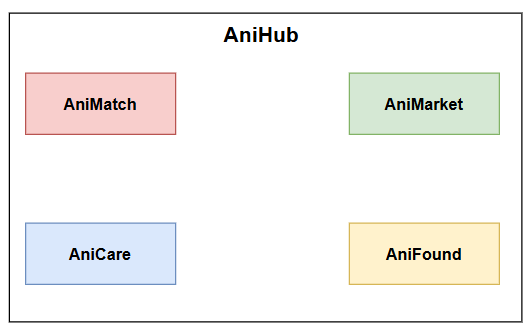
\includegraphics[width=0.7\textwidth]{images/squelette.png}
    \caption{Squelette fonctionnel de la plateforme AniHub}
    \label{fig:anihub-squelette}
\end{figure}

\noindent La plateforme AniHub s’articule autour de quatre modules principaux :

\begin{itemize}
    \item \textbf{AniMatch} : ce module est dédié à la mise en relation des propriétaires d’animaux dans un cadre structuré et sécurisé. Il facilite d’une part l’accouplement responsable des animaux en tenant compte de critères de compatibilité, et d’autre part l’adoption en permettant aux animaux de trouver de nouveaux foyers adaptés à leurs besoins, tout en favorisant une démarche responsable et encadrée.

    \item \textbf{AniMarket} : ce module constitue une marketplace spécialisée dans le domaine animalier. Il permet non seulement l’achat et la vente d’animaux domestiques, mais aussi la publication, la consultation et la gestion d’annonces relatives aux produits, accessoires et équipements destinés aux animaux, offrant ainsi un espace commercial complet et centralisé.

    \item \textbf{AniCare} : ce module regroupe un ensemble de services dédiés au bien-être et à la santé animale. Il met en relation les propriétaires avec des professionnels qualifiés tels que les vétérinaires, les dresseurs, les toiletteurs et les gardiens d’animaux, facilitant ainsi l’accès à des prestations fiables et adaptées aux besoins des animaux.

    \item \textbf{AniFound} : ce module est consacré à la gestion des animaux perdus et retrouvés. Il permet de signaler un animal perdu, de publier un animal retrouvé et de centraliser les informations afin de faciliter la mise en relation entre les utilisateurs concernés, augmentant ainsi les chances de retrouver rapidement les animaux disparus.
\end{itemize}

\newpage\subsection{Analyse comparative des solutions existantes et positionnement d’AniHub}

La table \ref{tab:comparison} présente une comparaison entre les solutions existantes en Tunisie et la plateforme \textbf{AniHub} selon différents critères fonctionnels et techniques, afin de mettre en évidence leurs limites et le positionnement d’AniHub : 
\renewcommand{\arraystretch}{1.3}

\begin{longtable}{|p{5.4cm}|p{2.8cm}|p{2.8cm}|p{2.8cm}|p{2.5cm}|}

\caption{Comparaison des solutions existantes avec AniHub}
\label{tab:comparison} \\

\hline
\rowcolor{coloranihub}
\textbf{Critère} & \textbf{Animaleries en ligne} & \textbf{Réseaux sociaux} & \textbf{Sites d’annonces} & \textbf{AniHub} \\
\hline
\endfirsthead

\hline
\rowcolor{coloranihub}
\textbf{Critère} & \textbf{Animaleries en ligne} & \textbf{Réseaux sociaux} & \textbf{Sites d’annonces} & \textbf{AniHub} \\
\hline
\endhead

Spécialisation animale & \ding{51} &  &  & \ding{51} \\
\hline

Large variété de produits pour animaux proposés & \ding{51} &  &  & \ding{51} \\
\hline

Facilité d’utilisation (UX/UI) & \ding{51} & \ding{51} & \ding{51} & \ding{51} \\
\hline

Degré de structuration des modules et des fonctionnalités & \ding{51} &  &  & \ding{51} \\
\hline

Modèle de vente entre particuliers (C2C) &  & \ding{51} & \ding{51} & \ding{51} \\
\hline

Disponibilité d'un système de matching pour reproduction animale &  &  &  & \ding{51} \\
\hline

Disponibilité des services dédiés aux animaux &  &  &  & \ding{51} \\
\hline

Disponibilité d’une section d’adoption des animaux &  &  &  & \ding{51} \\
\hline

Présence d’une fonctionnalité de marketplace &  &  &  & \ding{51} \\
\hline

Section de signalement des animaux perdus et retrouvés (Lost \& Found) &  &  &  & \ding{51} \\
\hline

\end{longtable}

\subsection{Objectifs de notre solution « AniHub »}

\begin{itemize}
\item \textbf{Objectifs humains :}  
À travers la solution AniHub, nous visons à promouvoir le bien-être animal en facilitant les adoptions responsables et en aidant les propriétaires à retrouver leurs animaux perdus.

\item \textbf{Objectifs intellectuels :}  
AniHub a pour objectif de favoriser l’échange et l’apprentissage autour du monde animal, grâce à une plateforme interactive permettant aux utilisateurs de partager des connaissances, poser des questions et enrichir leurs savoirs.

\item \textbf{Objectifs commerciaux :}  
La plateforme offre un espace dédié à la mise en relation entre vendeurs et acheteurs d’animaux, ainsi qu’aux prestataires de services (dresseurs, pet-sitters, vétérinaires et toiletteurs), afin d’élargir leur visibilité et d’attirer davantage de clients.
\end{itemize} 


\subsection{Public cible de la plateforme « AniHub »}

Notre plateforme s’adresse à un large éventail d’utilisateurs impliqués directement ou indirectement dans le domaine animalier. Elle vise notamment :

\begin{itemize}
    \item Les passionnés d’animaux et les professionnels du secteur animalier
    \item Les vendeurs d’animaux domestiques
    \item Les animaleries en Tunisie souhaitant publier leurs produits et articles
    \item Les personnes ayant perdu ou retrouvé un animal
    \item Les propriétaires souhaitant proposer leurs animaux à l’adoption
    \item Les propriétaires souhaitant faire reproduire (accoupler) leurs animaux dans un cadre adapté
    \item Les prestataires de services animaliers (vétérinaires, dresseurs, toiletteurs, gardiens)
\end{itemize} 

\subsection{Positionnement stratégique de la plateforme « AniHub »}
Notre plateforme \textbf{AniHub} ne se positionne pas comme un concurrent des animaleries en Tunisie, mais comme un partenaire visant à créer de la valeur pour l’ensemble des acteurs. Elle permet notamment aux petites boutiques sans présence en ligne de publier et promouvoir leurs produits.

Ainsi, AniHub offre un espace dédié pour améliorer leur visibilité et faciliter l’accès des propriétaires d’animaux à des produits et services de qualité. 
\section{Méthodologie de développement}

La réussite d’un projet dépend d’une méthodologie adaptée assurant le respect des délais et la satisfaction des besoins. Dans les projets à long terme, une communication continue avec le client est essentielle pour valider les livrables et intégrer les ajustements nécessaires.
\subsection{Comparaison des méthodes de travail} 
Les approches de développement logiciel se divisent en méthodes classiques, basées sur une planification rigide et une forte documentation, et en méthodes agiles, privilégiant la flexibilité, la collaboration et l’adaptation continue. Cette figure illustre cette différence : 
\begin{figure}[H]
\centering
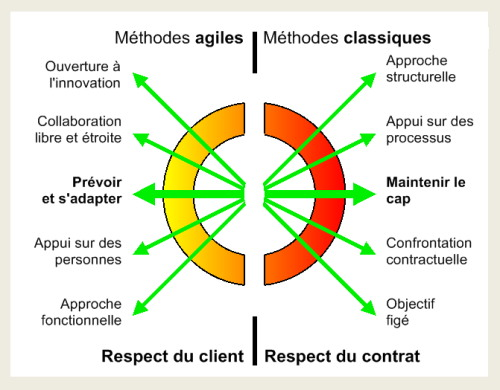
\includegraphics[width=0.6\linewidth, height=6.7cm]{images/comparaison.png}
\caption{Méthode Agile vs Méthode Classique \cite{agilevsclassic2017}}
\label{fig:classique_vs_agile}
\end{figure} 
\newpage 
\subsection{Méthodes agiles}

Après une comparaison des méthodes classiques et agiles, nous avons choisi une approche agile pour sa flexibilité. Une comparaison entre Scrum, Kanban et XP a ensuite été réalisée afin de sélectionner la méthode la plus adaptée à notre projet. 
\begin{longtable}{|p{4cm}|p{4cm}|p{4cm}|p{4cm}|}

\caption{Comparaison des méthodes agiles\cite{agile_comparatif_artza}} \\
\hline

\rowcolor{coloranihub}
\textbf{Critère} & \textbf{Scrum} & \textbf{Kanban} & \textbf{XP (Extreme Programming)} \\
\hline
\endfirsthead

\hline
\rowcolor{coloranihub}
\textbf{Critère} & \textbf{Scrum} & \textbf{Kanban} & \textbf{XP (Extreme Programming)} \\
\hline
\endhead

Organisation du travail & Basée sur des sprints & Flux continu & Itérations courtes \\
\hline

Planification & Fixée au début du sprint & Flexible et continue & Très fréquente et adaptative \\
\hline

Gestion des tâches & Backlog de sprint & Tableau Kanban (To Do / Doing / Done) & User stories détaillées \\
\hline

Rôles définis & Oui (Scrum Master, Product Owner, équipe) & Non obligatoire & Oui mais moins formalisés \\
\hline

Changement des exigences & Limité pendant le sprint & Accepté à tout moment & Accepté en continu \\
\hline

Livraison & À la fin de chaque sprint & Continue & Très fréquente \\
\hline

Qualité du code & Non spécifique & Non spécifique & Très forte (TDD, pair programming) \\
\hline

Implication client & Élevée à chaque sprint review & Variable & Très élevée et continue \\
\hline

Adapté pour & Projets structurés & Maintenance / flux continu & Projets techniques exigeants \\
\hline

\end{longtable}

\subsection{Méthodologie adoptée : Scrum}

Scrum est un cadre de travail agile permettant de gérer des projets complexes de manière itérative et incrémentale. Il repose sur une organisation structurée favorisant la collaboration, la transparence et l’adaptation continue tout au long du projet \cite{scrum_atlassian} . 
\subsubsection*{Équipe Scrum}

L’équipe Scrum est composée de plusieurs rôles complémentaires \cite{scrum_roles_atlassian} :

\begin{itemize}
    \item \textbf{Product Owner} : responsable de la définition des besoins du client et de la gestion du Product Backlog. Il priorise les fonctionnalités à développer.
    
    \item \textbf{Scrum Master} : garant du respect de la méthodologie Scrum. Il facilite le travail de l’équipe et élimine les obstacles rencontrés.
    
    \item \textbf{Équipe de développement} : composée des développeurs, elle est responsable de la conception, du développement et de la livraison du produit.
\end{itemize}

\subsubsection*{Les événements Scrum}

Scrum s’organise autour de plusieurs événements clés \cite{scrum_ceremonies_atlassian} :

\begin{itemize}
    \item \textbf{Sprint} : période courte (généralement 2 à 4 semaines) durant laquelle une version fonctionnelle du produit est développée.
    
    \item \textbf{Sprint Planning} : réunion de planification au début de chaque sprint pour définir les objectifs et les tâches à réaliser.
    
    \item \textbf{Daily Scrum (Daily Meeting)} : réunion quotidienne courte permettant de suivre l’avancement, identifier les obstacles et synchroniser l’équipe.
    
    \item \textbf{Sprint Review} : réunion en fin de sprint pour présenter les fonctionnalités développées au client et recueillir ses retours.
    
    \item \textbf{Sprint Retrospective} : réunion interne visant à analyser le sprint écoulé et à améliorer les processus de travail.
\end{itemize} 


\subsubsection*{Les artefacts Scrum (éléments clés)}

Les artefacts Scrum représentent les éléments essentiels du suivi du projet \cite{scrum_artifacts_atlassian} :

\begin{itemize}
    \item \textbf{Product Backlog} : liste priorisée de toutes les fonctionnalités et exigences du projet.
    
    \item \textbf{Sprint Backlog} : ensemble des tâches sélectionnées pour être réalisées durant un sprint.
    
    \item \textbf{Increment (Incrément)} : version fonctionnelle du produit livrée à la fin de chaque sprint, intégrant les nouvelles fonctionnalités développées.
\end{itemize} 
\subsubsection{Processus Scrum} 
La figure \ref{fig:scrum_process} illustre le processus de travail de Scrum , mettant en évidence les différentes étapes et interactions entre les rôles, les événements et les artefacts tout au long du projet : 
\begin{figure}[H]
\centering
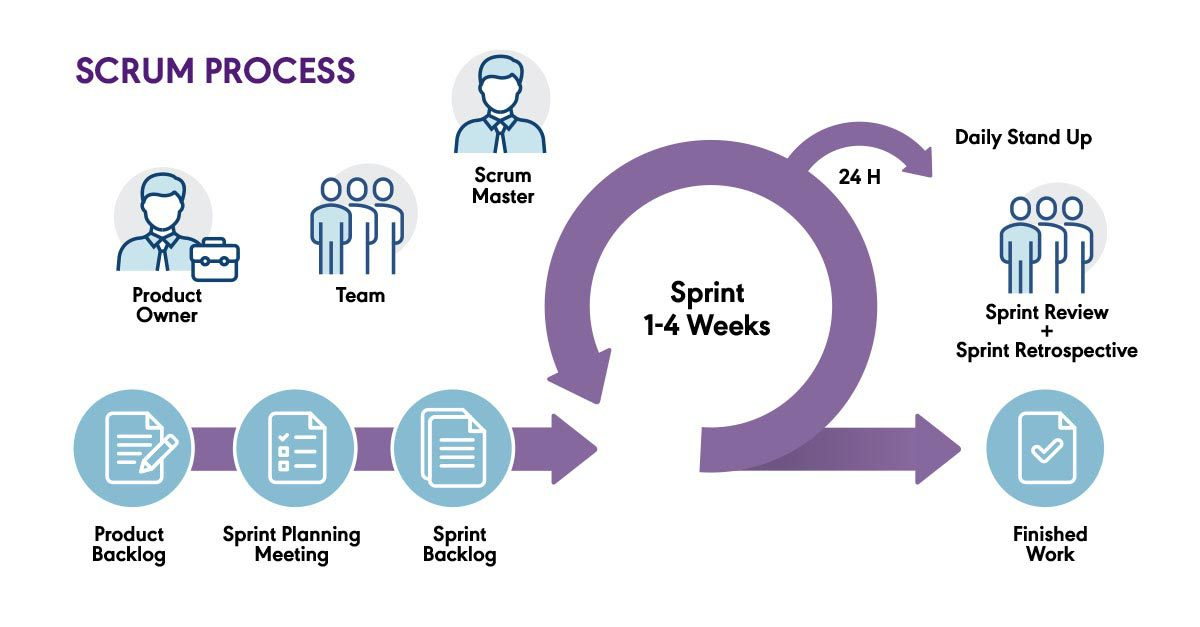
\includegraphics[width=0.9\linewidth, height=7cm]{images/scrum.jpg}
\caption{Processus de travail de Scrum \cite{scrum_process_pm}}
\label{fig:scrum_process}
\end{figure}  
Dans le cadre de notre projet, nous avons opté pour une planification basée sur la méthodologie Scrum, en définissant \textbf{6 sprints} répartis en \textbf{2 releases}. Cette organisation permet une progression incrémentale du développement, ainsi qu’une meilleure maîtrise des fonctionnalités livrées à chaque étape. Nous décrirons cette décomposition en détail à la fin du chapitre deux, après avoir présenté et défini l’ensemble des fonctionnalités du produit à réaliser.
\newpage 





\section{Chronogramme} 
La figure ci-dessous présente les différentes étapes de réalisation de notre projet, planifiées sur une période de stage de 4 mois, s’étendant du 1er février 2026 au 31 mai 2026.
\begin{figure*}[ht]
\centering
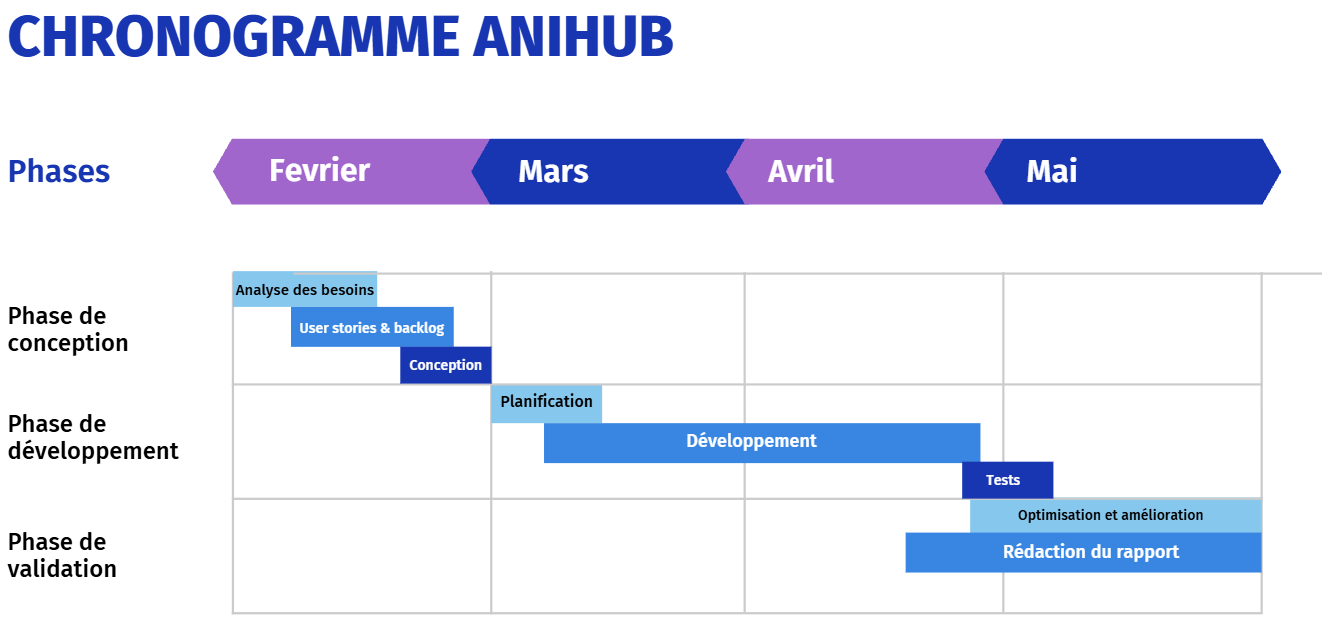
\includegraphics[width=0.95\linewidth, height=8cm]{images/chronogramme.png}
\caption{Chronogramme AniHub}
\label{fig:image}
\end{figure*}  

\section{Conclusion}

Dans ce chapitre, nous avons présenté le cadre général du projet AniHub ainsi que l’organisme d’accueil, AfterCode. Nous avons également réalisé une analyse de l’existant afin d’identifier les limites des solutions actuelles du marché des animaux domestiques en Tunisie. Sur cette base, nous avons proposé notre solution en détaillant ses principaux modules ainsi que ses objectifs et son positionnement stratégique. Enfin, nous avons introduit la méthodologie de développement adoptée, basée sur Scrum, qui structure le projet en plusieurs sprints et releases afin d’assurer un développement progressif et maîtrisé.

\chapter{Étude des besoins et planification du projet}
\label{chap:2}
\section{Introduction} 
L’étude des besoins représente une phase fondamentale précédant le développement d’un logiciel. Elle consiste à identifier les fonctionnalités ainsi que les propriétés que le système doit intégrer afin de satisfaire les attentes des utilisateurs. Dans ce chapitre, nous mettrons en évidence les besoins fonctionnels et non fonctionnels dans le but de concevoir une application à la fois performante et fiable. Nous définirons également les principaux acteurs du système et présenterons une vue d’ensemble de l’application, aussi bien sur le plan fonctionnel que technique, avant de terminer par la description de l’architecture adoptée. 

\section{Identification des acteurs} 
Comme évoqué précédemment, notre solution consiste en une plateforme web regroupant différents types d’utilisateurs. Elle fait intervenir plusieurs acteurs principaux, chacun jouant un rôle spécifique dans le fonctionnement du système : 
\begin{itemize}

\item \textbf{Utilisateur} : Cet acteur représente l’utilisateur de base de la plateforme. Il peut consulter l’ensemble des annonces disponibles (animaux à vendre, animaux pour accouplement, animaux en adoption, services animaliers, ainsi que les déclarations de perte et de trouvaille). Il a également la possibilité de gérer son compte personnel, de publier des annonces pour proposer son animal à l’accouplement ou à l’adoption, ainsi que de publier des annonces de perte ou de trouvaille d’animaux.

\item \textbf{Prestataire de service} : Cet acteur hérite de l’acteur \textbf{Utilisateur}. Il peut s’agir d’un dresseur d’animaux, d’un vétérinaire, d’un gardien d’animaux ou d’un toiletteur. En plus des fonctionnalités de base, il peut créer, modifier et gérer ses annonces de services destinés aux animaux afin de proposer ses prestations sur la plateforme.

\item \textbf{Vendeur} : Cet acteur hérite également de l’acteur \textbf{Utilisateur}. Il a la possibilité de mettre en vente des animaux, soit via un système d’enchères, soit à prix fixe. Il peut également gérer ses annonces de vente (ajout, modification, suppression).

\item \textbf{Administrateur} : Il est responsable de la gestion globale de la plateforme. Il peut gérer tous les utilisateurs ainsi que toutes les annonces (vente d’animaux, accouplement, adoption, services et déclarations de perte et de trouvaille). Il dispose également de droits de modération afin de garantir la qualité et la sécurité du contenu publié.

\end{itemize}

\section{Besoins Fonctionnels} 
\subsection{Pour un utilisateur}

Lorsqu’un utilisateur accède à notre plateforme, il peut effectuer les actions suivantes :

\begin{itemize}
    \item S’inscrire et créer un compte.
    \item Consulter l’ensemble du contenu disponible sur la plateforme.
    \item Gérer son compte (modifier ou supprimer ses informations personnelles).
    \item Gérer ses déclarations de perte ou de trouvaille d’animaux (ajouter, modifier, supprimer).
    \item Gérer ses annonces d’animaux destinés à l’accouplement (ajouter, modifier, supprimer).
    \item Gérer ses annonces d’animaux destinés à l’adoption (ajouter, modifier, supprimer).
    \item Gérer ses envois, notamment : demandes d’accouplement, demandes d’adoption, indices liés aux déclarations de trouvaille d’animaux, offres pour les enchères et réservations de services.
    \item Gérer ses réceptions, telles que : intérêts reçus pour l’accouplement, intérêts reçus pour l’adoption et indices reçus concernant les déclarations de trouvaille d’animaux.
\end{itemize} 

\subsection{Pour un vendeur}

Lorsqu’un vendeur accède à notre plateforme, et puisqu’il hérite du rôle d’utilisateur, il dispose de l’ensemble des fonctionnalités offertes à un utilisateur. En plus de cela, il peut également :

\begin{itemize}
    \item Gérer ses animaux à vendre (ajouter, modifier et supprimer), que ce soit à prix fixe ou sous forme d’enchères. 
    \item Gérer les offres reçues pour ses enchères.
    \item Gérer ses produits à vendre (ajouter, modifier et supprimer).
\end{itemize} 


\subsection{Pour un prestataire de service} 
Lorsqu’un prestataire de service accède à notre plateforme,et puisqu’il hérite du rôle d’utilisateur, il dispose de l’ensemble des fonctionnalités offertes à un utilisateur. En plus de cela, il peut également : 
\begin{itemize}
    \item Gérer (ajouter ,modifier , supprimer) ses annonces de service (Véterinaire , dressage , toilettage , garderie ) pour animaux . 
    \item Consulter et gérer les demandes de réservation effectuées par les utilisateurs pour ses services.
\end{itemize} 
\subsection{Pour un administrateur}

Lorsqu’un administrateur accède à la plateforme, il peut effectuer les actions suivantes :

\begin{itemize}
    \item Consulter son tableau de bord et gérer l’ensemble des éléments de la plateforme, notamment : les utilisateurs, les animaux à vendre, les animaux destinés à l’accouplement, les animaux proposés à l’adoption, les services animaliers, ainsi que les déclarations de perte et de trouvaille.
\end{itemize} 

\section{Besoins non fonctionnels}

Dans une architecture distribuée composée de services indépendants, les besoins non fonctionnels sont essentiels pour garantir la qualité, la fiabilité et l’efficacité globale du système. Ils définissent les contraintes que la plateforme doit respecter afin d’assurer une expérience utilisateur optimale et un fonctionnement robuste.

\begin{itemize}

    \item \textbf{Ergonomie et expérience utilisateur} : Proposer une interface simple, intuitive et cohérente, permettant aux utilisateurs de naviguer facilement et d’accéder rapidement aux différentes fonctionnalités. L’objectif est de garantir une expérience fluide, agréable et adaptée à différents supports.

    \item \textbf{Scalabilité} : Assurer la capacité du système à supporter une augmentation progressive ou soudaine du nombre d’utilisateurs et de requêtes, sans dégradation des performances. Chaque composant doit pouvoir évoluer de manière indépendante selon la charge.

    \item \textbf{Disponibilité} : Garantir un accès continu aux services de la plateforme avec un minimum d’interruptions. Le système doit rester fonctionnel même en cas de perturbation partielle de certains composants.

    \item \textbf{Résilience et tolérance aux pannes} : Assurer la continuité du service même en cas de défaillance d’un ou plusieurs composants. Le système doit être capable d’isoler les erreurs et de maintenir les fonctionnalités critiques opérationnelles.

    \item \textbf{Performance} : Optimiser les temps de réponse et assurer un traitement efficace des requêtes, même dans des conditions de forte charge ou de communication entre plusieurs composants.

    \item \textbf{Sécurité} : Protéger les données et contrôler strictement les accès aux différentes fonctionnalités. Le système doit garantir la confidentialité, l’intégrité et la disponibilité des informations échangées.

    \item \textbf{Maintenabilité} : Faciliter l’évolution du système, la correction des anomalies et l’ajout de nouvelles fonctionnalités. Une bonne organisation interne doit permettre des modifications sans impact global sur la plateforme.

    \item \textbf{Observabilité} : Permettre le suivi du comportement global du système afin de détecter rapidement les anomalies, analyser les performances et faciliter le diagnostic des problèmes.

    \item \textbf{Interopérabilité} : Assurer une communication fluide entre les différentes parties du système ainsi qu’avec des services externes, à travers des interfaces bien définies.

\end{itemize}
\section{Diagramme de cas d’utilisation global}  
Nous allons illustrer le fonctionnement de notre solution pour chaque acteur à l’aide d’un diagramme de cas d’utilisation. Ce diagramme permet de représenter les interactions entre les différents acteurs et le système, afin de mieux comprendre leur rôle et leur relation avec la plateforme.

Cette figure présente le diagramme global des cas d’utilisation de notre plateforme : 
\begin{figure}[H]
    \centering
    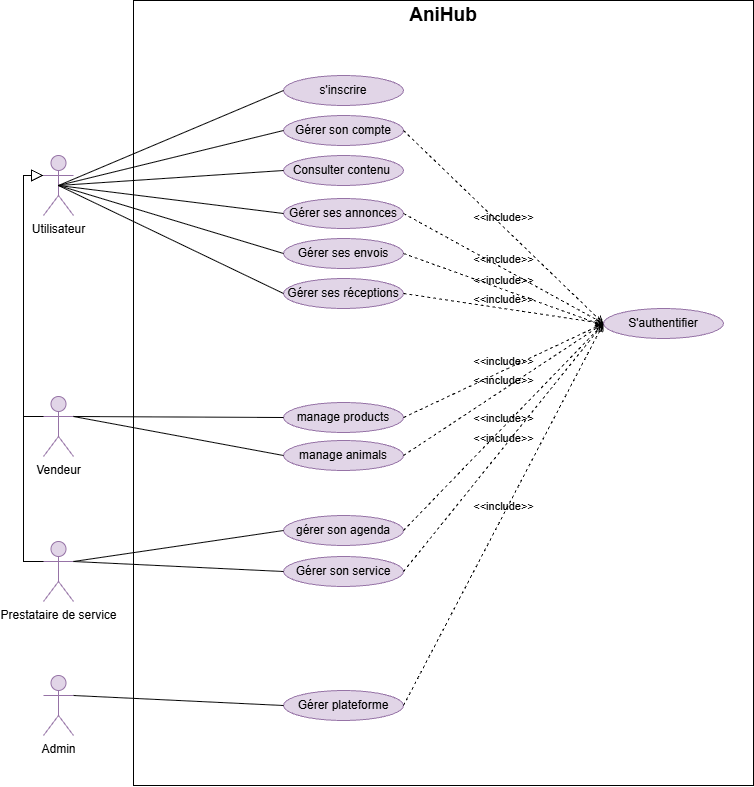
\includegraphics[width=0.94\textwidth]{images/usecase (2).png}
    \caption{Diagramme de cas d'utilisation général}
\end{figure} 
\section{Architecture globale du projet}

Dans cette section, nous présentons l’architecture générale adoptée pour le projet. Nous décrivons d’abord les architectures monolithique et microservices, puis nous les comparons afin de justifier le choix retenu. Enfin, nous détaillons l’architecture globale du système ainsi que ses principaux composants. 
\newpage 
\subsection{Architecture monolithique}

\subsubsection{Principe}
L’architecture monolithique regroupe toutes les fonctionnalités d’une application (interface utilisateur, logique métier et accès aux données) dans une seule unité de déploiement, fortement couplée et exécutée dans un même processus.

\subsubsection{Avantages}
\begin{itemize}
    \item Simplicité de développement et de déploiement.
    \item Facilité de test et de gestion dans les petits projets.
    \item Centralisation du code et des dépendances.
\end{itemize}

\subsubsection{Inconvénients}
\begin{itemize}
    \item Difficulté de maintenance lorsque le système devient complexe.
    \item Faible scalabilité.
    \item Redéploiement complet nécessaire à chaque modification.
\end{itemize}

\subsubsection{Cas d’utilisation}
Cette architecture est adaptée aux petites applications, aux prototypes ou aux projets avec une faible complexité et un nombre limité de fonctionnalités.

\subsection{Architecture microservices}

\subsubsection{Principe}
L’architecture microservices est une approche dans laquelle une application est décomposée en plusieurs services indépendants, chacun responsable d’une fonctionnalité métier spécifique. Chaque service est autonome et communique avec les autres via des API.

\subsubsection{Avantages}
\begin{itemize}
    \item Forte modularité et indépendance des services.
    \item Scalabilité indépendante de chaque composant.
    \item Déploiement et mise à jour sans impacter tout le système.
\end{itemize}

\subsubsection{Inconvénients}
\begin{itemize}
    \item Complexité de gestion et de déploiement.
    \item Communication réseau entre services.
    \item Besoin d’une infrastructure plus avancée.
\end{itemize}

\subsubsection{Cas d’utilisation}
Cette architecture est adaptée aux systèmes complexes, aux plateformes évolutives, aux applications distribuées et aux projets nécessitant une forte scalabilité.
\newpage
\subsection{Comparaison entre architecture monolithique et microservices}

Cette section présente une comparaison entre les architectures monolithique et microservices afin de mettre en évidence leurs principales différences.

La figure ci-dessous illustre le contraste entre une application centralisée et une architecture distribuée en services indépendants.

\begin{figure}[H]
    \centering
    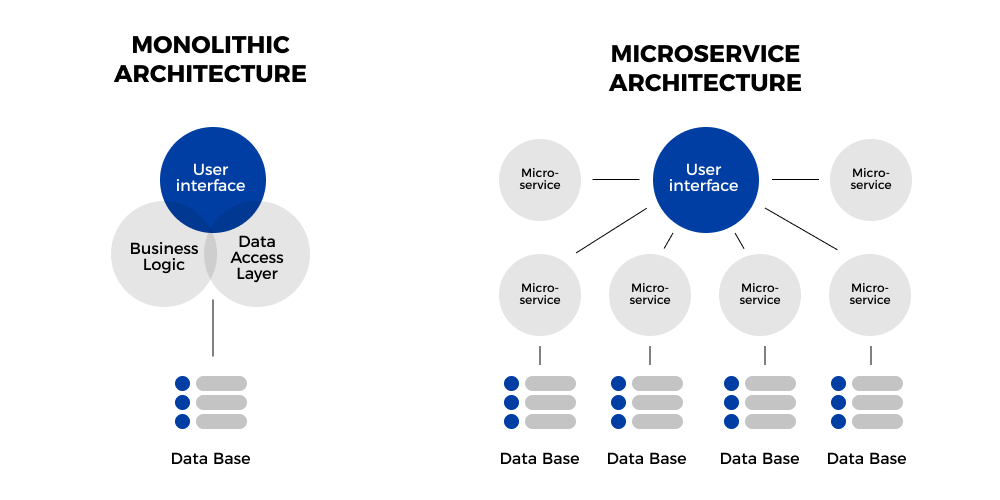
\includegraphics[width=0.9\linewidth]{images/micro vs mono.png}
    \caption{Comparaison architecture monolithique vs microservices}
\end{figure}

Le tableau ci-dessous illustre une comparaison détaillée entre les deux architectures selon plusieurs critères.


\begin{longtable}{|p{3.5cm}|p{6cm}|p{6cm}|}
\hline
\rowcolor{coloranihub}
\textbf{Critères} & \textbf{Architecture monolithique} & \textbf{Architecture microservices} \\
\hline
Structure & Application unique & Services indépendants \\
\hline
Déploiement & Global & Par service \\
\hline
Scalabilité & Limitée & Flexible et fine \\
\hline
Maintenance & Complexe avec la taille & Simplifiée par modularité \\
\hline
Évolution & Impact global & Indépendante par service \\
\hline
Technologies & Homogènes & Hétérogènes possibles \\
\hline
Performance & Adaptée aux petits systèmes & Optimisée pour systèmes distribués \\
\hline
Tolérance aux pannes & Impact global & Isolation des pannes \\
\hline
Complexité & Faible au départ & Plus élevée \\
\hline
Organisation des équipes & Centralisée & Distribuée \\
\hline
\end{longtable}

Ainsi, l’architecture microservices offre une meilleure flexibilité et évolutivité, tandis que l’architecture monolithique reste plus simple à mettre en place pour des systèmes de petite taille.
\subsection{Choix de l’architecture du projet}
\subsubsection{Justification du choix de l’architecture microservices}

Dans notre projet, nous avons opté pour l’architecture microservices pour les raisons suivantes.

\begin{itemize}

\item \textbf{Découpage fonctionnel :} \textbf{"AniHub"} regroupe plusieurs modules indépendants (marketplace, services de bien-être animal, adoption, accouplement, aide à la découverte des animaux perdus). Par exemple, la gestion des annonces d’adoption est indépendante du module marketplace, ce qui justifie une séparation en services. 
\item 
\item \textbf{Évolutivité :} \textbf{"AniHub"} étant une première version évolutive, de nouvelles fonctionnalités telles que le web scraping ou un module d’IA peuvent être ajoutées sans impacter les services existants.

\item \textbf{Résilience :} dans \textbf{"AniHub"}, une panne d’un service comme le module marketplace n’affecte pas les autres fonctionnalités (ex : le module d'accouplement).

\item \textbf{Scalabilité :} certains modules de \textbf{"AniHub"}, tels que le marketplace ou les services de bien-être animal, peuvent être plus sollicités et nécessitent une montée en charge indépendante.
\end{itemize}
\subsubsection{Présentation de notre architecture}

Cette figure illustre la structure générale de l’architecture microservices d’AniHub.

\begin{figure}[H]
    \centering
    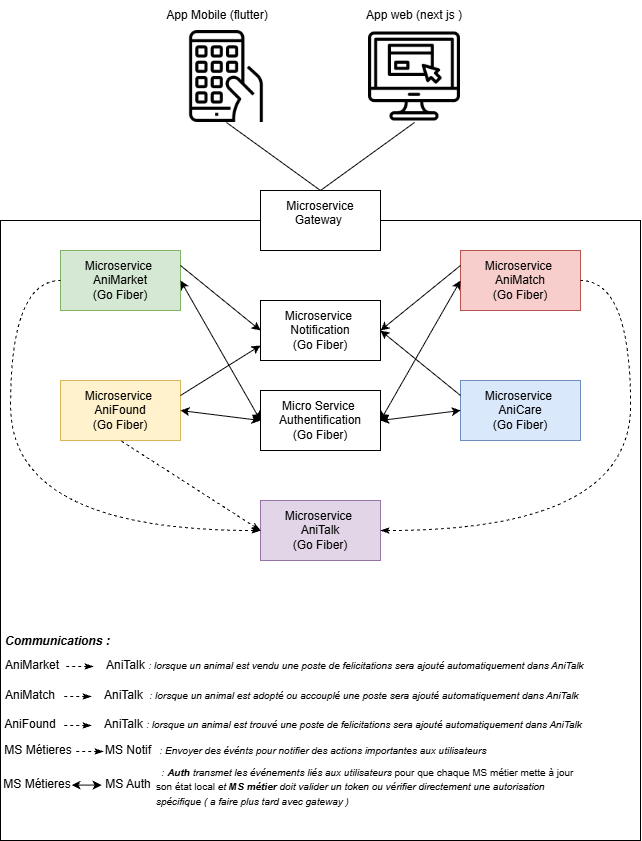
\includegraphics[width=0.5\linewidth]{images/Présentation de notre architecture.png}
    \caption{Présentation de notre architecture}
    \label{fig:arch_anihub}
\end{figure}


Les applications clientes, développées avec \textbf{Next.js} pour le web et \textbf{Flutter} pour le mobile, accèdent au système via un \textbf{API Gateway}, qui assure le routage des requêtes vers les microservices concernés.

\vspace{0.3cm}

L’architecture est composée de plusieurs microservices métiers développés avec \textbf{Go Fiber}, tels que :

\begin{itemize}
    \item \textbf{AniMatch} : gestion de l’adoption et de la mise en relation entre animaux.
    \item \textbf{AniMarket} : marketplace des produits animaliers.
    \item \textbf{AniFound} : gestion des animaux perdus et retrouvés.
    \item \textbf{AniCare} : services et soins animaliers.
    \item \textbf{AniTalk} : espace de communication et d’échanges.
\end{itemize}

\vspace{0.3cm}



\section{Stack technologique et outils de développement} 
\subsection{Outils et environnement de développement}

\subsubsection{Slack}
\begin{center}
    
\includegraphics[width=2cm]{images/slack.png}
\end{center}
Slack est une plateforme de communication collaborative permettant aux équipes de discuter, partager des fichiers et organiser le travail via des canaux dédiés.

\vspace{0.3cm}

\subsubsection{draw.io}
\begin{center}
    
\includegraphics[width=2cm]{images/drawio.png}
\end{center}
draw.io est un outil en ligne permettant de créer facilement des diagrammes tels que les diagrammes UML, les organigrammes et les schémas d’architecture.

\vspace{0.3cm}

\subsubsection{Figma}
\begin{center}
    
\includegraphics[width=1.5cm]{images/figma.png}
\end{center}
Figma est un outil de conception d’interfaces utilisateur (UI/UX) collaboratif, utilisé pour créer des maquettes, prototypes et designs interactifs.

\vspace{0.3cm}

\subsubsection{Visual Studio Code}
\begin{center}
    
\includegraphics[width=2cm]{images/vscode.png}
\end{center}
Visual Studio Code est un éditeur de code source léger et puissant, supportant plusieurs langages de programmation et offrant des extensions pour améliorer la productivité des développeurs.

\vspace{0.3cm}

\subsubsection{Git et GitHub}

\begin{center}
\begin{minipage}{0.45\textwidth}
    \centering
    
\includegraphics[width=2cm]{images/git.png}
    
    \textbf{Git}
\end{minipage}
\hfill
\begin{minipage}{0.45\textwidth}
    \centering
    
\includegraphics[width=2cm]{images/github.png}
    
    \textbf{GitHub}
\end{minipage}
\end{center}

Git est un système de gestion de versions distribué permettant de suivre les modifications du code source, de gérer les différentes versions d’un projet et de faciliter le travail collaboratif entre les développeurs. GitHub est une plateforme d’hébergement de code basée sur Git, offrant des fonctionnalités de collaboration telles que le partage de dépôts, la gestion des versions, le suivi des problèmes (issues) et l’intégration continue.

\subsubsection{GitHub Actions}
\begin{center}
    
\includegraphics[width=7cm]{images/githubActions.png}
\end{center} 


GitHub Actions est un outil d’intégration et de déploiement continu (CI/CD) permettant d’automatiser les tâches de build, de test et de déploiement des applications directement depuis les dépôts GitHub.


\subsection{Stack technologique}

\subsubsection{TypeScript}
\begin{center}
    
\includegraphics[width=2cm]{images/typescript.png}
\end{center}
TypeScript est un langage de programmation basé sur JavaScript qui ajoute le typage statique, permettant de rendre le code plus robuste, maintenable et moins sujet aux erreurs.

\vspace{0.3cm}

\subsubsection{Next.js}
\begin{center}
    
\includegraphics[width=2cm]{images/nextjs.png}
\end{center}
Next.js est un framework basé sur React permettant de développer des applications web modernes avec rendu côté serveur (SSR), génération statique (SSG) et optimisation des performances.

\vspace{0.3cm}

\subsubsection{Tailwind CSS}
\begin{center}
    
\includegraphics[width=2.7cm]{images/tailwind.png}
\end{center}
Tailwind CSS est un framework CSS utilitaire permettant de concevoir rapidement des interfaces modernes et responsives sans écrire de CSS personnalisé complexe.

\vspace{0.3cm}

\subsubsection{Go et Fiber}

\begin{center}
\begin{minipage}{0.45\textwidth}
    \centering
    
\includegraphics[width=3cm]{images/go.png}
    
\end{minipage}
\hfill
\begin{minipage}{0.45\textwidth}
    \centering
    
\includegraphics[width=3cm]{images/fiber.png}
    
\end{minipage}
\end{center}

Go est un langage de programmation compilé développé par Google, reconnu pour sa simplicité, sa performance et sa gestion efficace de la concurrence. Fiber est un framework web rapide pour Go, inspiré d’Express.js, facilitant la création d’API performantes et légères. 

\subsubsection{Neon PostgreSQL}
\begin{center}
    
\includegraphics[width=3cm]{images/neon.jpg}
\end{center}
Neon PostgreSQL est une plateforme de base de données serverless basée sur PostgreSQL, offrant scalabilité, performance et séparation du stockage et du calcul.

\vspace{0.3cm} 


 \subsubsection{Postman}

\begin{center}
    
\includegraphics[width=4cm]{images/postman.png}
\end{center}

Postman est un outil de test et de développement d’API permettant d’envoyer des requêtes HTTP, de vérifier les réponses des services et de faciliter le débogage des interfaces backend.

\subsubsection{RabbitMQ}

\begin{center}
    
\includegraphics[width=4cm]{images/rabbit.png}
\end{center} 



RabbitMQ est un système de messagerie (message broker) permettant la communication asynchrone entre les différents services d’une architecture distribuée. Il facilite l’échange de messages entre producteurs et consommateurs afin d’assurer un découplage des composants, une meilleure scalabilité et une gestion efficace des traitements en arrière-plan. 
\subsubsection{Docker}
\begin{center}
    
\includegraphics[width=3.4cm]{images/docker.png}
\end{center}
Docker est une plateforme de conteneurisation permettant d’emballer les applications et leurs dépendances afin d’assurer leur portabilité et leur déploiement rapide.

\vspace{0.3cm}

\subsubsection{Kubernetes}
\begin{center}
    
\includegraphics[width=2.8cm]{images/k8s.png}
\end{center}
Kubernetes est un système d’orchestration de conteneurs permettant de déployer, gérer et scaler automatiquement des applications conteneurisées. 

\section{Pilotage du projet : méthode Scrum} 
Comme mentionné précédemment, la méthodologie Scrum a été retenue pour ce projet. 
\subsection{Équipe et rôles} 
La figure ci-dessous illustre les différentes parties prenantes de l’application : 
\begin{figure}[H]
    \centering
    
\includegraphics[width=0.92\linewidth]{images/scrumteam.png}
    \caption{Équipe et rôles Scrum}
\end{figure}\newpage 





\subsection{Backlog produit} 
Le backlog Scrum regroupe les user stories priorisées du projet. Le tableau ci-dessous présente le backlog produit.
\begin{longtable}{|p{4cm}|p{9.5cm}|p{2cm}|} 
\caption{Backlog produit}\label{tab:product-backlog}\\
\hline
\rowcolor{coloranihub}
\textbf{Product Backlog Item (Sprint)} & \textbf{User Story} & \textbf{Priorité} \\
\hline
\endfirsthead

\hline
\rowcolor{coloranihub}
\textbf{Product Backlog Item (Sprint)} & \textbf{User Story} & \textbf{Priorité} \\
\hline
\endhead

\hline
\endfoot

\multirow{5}{4cm}{\textbf{Sprint 1 : Authentification et administration}} 
& En tant qu'utilisateur, je veux accéder à une interface moderne et intuitive, afin de naviguer facilement sur AniHub. & Must Have \\
\cline{2-3}
& En tant qu'utilisateur, je veux créer un compte et me connecter afin d'accéder à la plateforme & Must Have \\
\cline{2-3}
& En tant qu'utilisateur, je veux gérer mon profil afin de personnaliser mes informations & Should Have \\
\cline{2-3}
& En tant qu'administrateur, je veux gérer tous les utilisateurs afin de superviser la plateforme & Must Have \\
\cline{2-3}
& En tant qu'administrateur, je veux gérer toutes les annonces (animaux, déclarations, services) afin de superviser et contrôler le contenu de la plateforme & Must Have \\
\hline
% ===================== SPRINT 2ANIMATCH=====================
\multirow{9}{4cm}{\textbf{Sprint 2 : Module AniMatch}}
& En tant qu’utilisateur, je veux consulter la liste des animaux (adoption ou accouplement) afin de trouver un partenaire compatible & Must Have \\
\cline{2-3}
& En tant qu’utilisateur, je veux gérer mes annonces afin de les publier, modifier et supprimer. & Must Have \\
\cline{2-3}
& En tant qu’utilisateu,je veux gérer mes invitations envoyées pour suivre mes interactions, publier , modifier ou annuler une demande d'adoption ou accouplement & Must Have \\
\cline{2-3}
& En tant qu’utilisateur, je veux gérer les invitations reçues pour adoption ou accouplement afin de répondre aux demandes, accepter ou refuser les propositions et organiser mes interactions. & Must Have \\
\cline{2-3}
& En tant qu'utilisateur, je veux gérer mes notifications afin d’être informé en temps réel des interactions liées à mes annonces et activités sur \textbf{AniMatch} & Should Have \\
\cline{2-3}
& En tant qu'utilisateur, je veux discuter avec un autre propriétaire afin de finaliser une adoption ou un accouplement & Should Have \\
\hline
% ===================== SPRINT 3 : ANIFOUND =====================
\multirow{8}{4cm}{\textbf{Sprint 3 : Module AniFound}}
& En tant qu’utilisateur, je souhaite consulter les déclarations de perte et de trouvaille afin de retrouver ou identifier un animal & Must Have \\
\cline{2-3}
& En tant qu'utilisateur, je veux gérer mes déclarations de perte (modifier/supprimer) afin de mettre à jour mes informations & Must Have \\
\cline{2-3}
& En tant qu’utilisateur, je veux envoyer, gérer, modifier, annuler et suivre le statut de mes indices afin de prouver qu’il s’agit bien de mon animal. & Must Have \\
\cline{2-3}
& En tant qu’utilisateur, je veux gérer les indices reçus afin de les examiner et d’y répondre (acceptation ou refus) & Must Have \\
\cline{2-3}
& En tant qu’utilisateur, je veux gérer mes notifications afin d’être informé des interactions sur mes déclarations de perte, de trouvaille et de mes indices. & Should Have \\
\cline{2-3}
& En tant qu’utilisateur, je veux contacter l’autre partie afin d’échanger des informations et faciliter la résolution de la situation & Should Have \\
\hline
% ===================== SPRINT 4 : ANIMARKET =====================
\multirow{10}{4cm}{\textbf{Sprint 4 : Module AniMarket}}
&En tant qu’utilisateur, je veux consulter la liste des animaux à vendre afin de découvrir les annonces disponibles et comparer les différentes offres proposée & Must Have \\
\cline{2-3}

& En tant qu’utilisateur, je veux proposer une offre sur une enchère afin de participer au processus d’achat et tenter d’acquérir un animal & Must Have \\
\cline{2-3}

& En tant qu’utilisateur, je veux gérer mes notifications afin d’être informé des interactions sur mes annonces et activités (offres, enchères, wishlist) et suivre les mises à jour en temps réel & Should Have \\
\cline{2-3}

& En tant que vendeur, je veux gérer mes animaux à vendre afin de maintenir mes annonces à jour, les publier, les modifier ou les supprimer selon leur disponibilité & Must Have \\
\cline{2-3}
& En tant que vendeur, je veux gérer les offres reçues afin de les consulter, les accepter ou les refuser selon les propositions des acheteurs  & Must Have \\
\cline{2-3}

& En tant qu’utilisateur, je veux commenter et noter un animal afin de partager mon avis et évaluer les annonces consultées  & Could Have \\
\cline{2-3}

& En tant qu’utilisateur, je veux discuter avec le vendeur afin d’échanger des informations complémentaires et faciliter la transaction  & Should Have \\
\hline
% ===================== SPRINT 5 : ANICARE =====================
\multirow{8}{4cm}{\textbf{Sprint 5 : Module AniCare}}
& En tant qu’utilisateur, je souhaite consulter la liste des services afin de découvrir les services disponibles et choisir celui qui correspond le mieux à mes besoins & Must Have \\
\cline{2-3}

& En tant qu’utilisateur, je souhaite gérer mes réservations envoyées (envoyer, suivre, modifier, annuler) afin de gérer efficacement mes demandes & Must Have \\
\cline{2-3}

& En tant qu’utilisateur, je souhaite gérer mes notifications afin d’être informé des interactions sur mes activités & Should Have \\
\cline{2-3}

& En tant qu’utilisateur, je souhaite discuter avec l’autre partie (utilisateur ou prestataire) afin de faciliter la communication & Should Have \\
\cline{2-3}

& En tant que prestataire de service, je souhaite gérer mon propre service (publier, mettre à jour, supprimer) afin de présenter mes services de manière claire & Must Have \\
\cline{2-3}

& En tant que prestataire de service, je souhaite gérer mes réservations reçues afin de répondre aux demandes des clients et organiser efficacement mes prestations & Must Have \\
\cline{2-3}

& En tant que prestataire de service, je souhaite gérer mes cours afin de les organiser, les publier et les mettre à jour selon mes besoins & Won’t Have \\
\cline{2-3}

& En tant qu’utilisateur, je souhaite consulter les cours des prestataires de service afin de découvrir les contenus disponibles et apprendre selon mes besoins & Won’t Have \\
\hline 

% ===================== SPRINT 6 : DEVOPS =====================
\multirow{4}{4cm}{\textbf{Sprint 6 : Conteneurisation, CI/CD, Déploiement Cloud et Monitoring}}
& Conteneuriser les microservices avec Docker afin de garantir un environnement d’exécution stable et portable & Must Have \\
\cline{2-3}
& Déployer les microservices sur Kubernetes afin d’assurer l’orchestration et la disponibilité de l’application. & Must Have \\
\cline{2-3}
& Déployer l’application sur Google Cloud Platform (GCP) afin de rendre la plateforme accessible en ligne. & Must Have \\
\cline{2-3}
& Automatiser le build et le déploiement avec GitHub Actions afin d’assurer un processus CI/CD rapide et fiable. & Should Have \\  
\cline{2-3}
& Surveiller les microservices avec Grafana afin de suivre les performances et détecter les anomalies du système. & Could Have \\
\hline


\end{longtable} 


\subsection{Méthode de priorisation MoSCoW}

La priorisation des besoins est réalisée selon la méthode MoSCoW. Le tableau ci-dessous illustre les différentes catégories de cette méthode : 


\definecolor{coloranihub}{HTML}{E1D5E7}

\begin{longtable}{|p{3.5cm}|p{12cm}|}
\caption{Catégories de la méthode MoSCoW}
\label{tab:moscow} \\
\hline
\rowcolor{coloranihub}
\textbf{Catégorie} & \textbf{Description} \\
\hline
\endfirsthead

\hline
\rowcolor{coloranihub}
\textbf{Catégorie} & \textbf{Description} \\
\hline
\endhead

\textbf{Must Have} & Fonctionnalités essentielles au bon fonctionnement du système, sans lesquelles le produit ne peut pas fonctionner correctement. \\
\hline

\textbf{Should Have} & Fonctionnalités importantes mais non essentielles. Elles améliorent le système, sans être indispensables à son fonctionnement. \\
\hline

\textbf{Could Have} & IFonctionnalités optionnelles qui améliorent l’expérience utilisateur, sans être nécessaires dans la première version. \\
\hline

\textbf{Won’t Have} & Fonctionnalités non retenues pour cette version du projet, en raison de contraintes de temps, de ressources ou de priorité. \\
\hline

\end{longtable}

\newpage
\subsection{Planification des sprints et des releases}

Le tableau ci-dessous présente la planification des sprints ainsi que des releases du projet : 

\renewcommand{\arraystretch}{1.5}

\begin{longtable}{|m{4cm}|m{4cm}|m{6cm}|>{\centering\arraybackslash}m{2cm}|}
\caption{Planification des sprints et des releases} \\
\hline
\rowcolor{coloranihub}
\textbf{Release} & \textbf{Sprint} & \textbf{Description} & \textbf{Durée} \\
\hline
\endfirsthead

\hline
\rowcolor{coloranihub}
\textbf{Release} & \textbf{Sprint} & \textbf{Description} & \textbf{Durée} \\
\hline
\endhead

\multirow{3}{4cm}{\textbf{Release 1 : AniHub partie 1}} 
& Sprint 1 : Authentification et Administration 
& Gestion de l’inscription, de la connexion, des rôles ainsi que du tableau de bord administrateur 
& 2 semaines \\
\cline{2-4}

& Sprint 2 : AniMatch 
& Module dédié à la mise en relation pour l’adoption et l’accouplement des animaux 
& 3 semaines \\
\cline{2-4}

& Sprint 3 : AniFound 
& Module permettant la déclaration et la recherche des animaux perdus 
& 3 semaines \\
\hline

\multirow{3}{4cm}{\textbf{Release 2 : AniHub partie 2}} 
& Sprint 4 : AniMarket 
& Gestion des annonces de vente de produits et services liés aux animaux 
& 3 semaines \\
\cline{2-4}

& Sprint 5 : AniCare 
& Gestion des services de soins et du suivi des animaux 
& 3 semaines \\
\cline{2-4}

& Sprint 6 : Conteneurisation, CI/CD, Déploiement et Monitoring 
& Phase de déploiement de l’application, tests finaux et correction des anomalies 
& 2 semaines \\
\hline

\end{longtable} 
\section{Conclusion}

Dans ce chapitre, nous avons présenté l’étude des besoins de la plateforme \textbf{AniHub}, les différents acteurs ainsi que les besoins fonctionnels et non fonctionnels du système. Nous avons également présenté l’architecture microservices adoptée, les technologies utilisées ainsi que l’organisation du projet selon la méthode Scrum, incluant le backlog produit, la planification des sprints et des releases. Cette étude constitue une base essentielle pour la conception et la réalisation de notre application. 








\chapter{Release 1 : AniHub partie 1 } 
\label{chap:3}
\section{Introduction}

La première release est dédiée aux fonctionnalités de la plateforme et à la mise en relation entre utilisateurs. Elle comprend un module d’authentification et d’administration, ainsi que les modules AniMatch, pour l’adoption et l’accouplement des animaux, et AniFound, pour la recherche des animaux perdus.

Cette release est réalisée à travers trois sprints :
\begin{itemize}
    \item \textbf{Sprint 1 : Authentification \& Administration}
    \item \textbf{Sprint 2 : Module AniMatch}
    \item \textbf{Sprint 3 : Module AniFound}
\end{itemize}


 
\section{Sprint 1 : Authentification et administration} Ce sprint, d’une durée de \textbf{deux semaines}, est consacré à la mise en place des fonctionnalités d’authentification et d’administration. Il permet d’assurer un accès sécurisé à la plateforme via la gestion des comptes utilisateurs (inscription, connexion et contrôle des rôles), ainsi que la mise en place d’un espace d’administration pour superviser le système et garantir la cohérence des opérations. 
\subsection{Sprint backlog} 
La table \ref{tab:sprint1-backlog} présente le Sprint Backlog du sprint 1 avec les user stories, les tâches associées et les efforts estimés :

\begin{longtable}{|p{1cm}|p{4.7cm}|p{7cm}|p{1.3cm}|}

\caption{Sprint Backlog du sprint 1}
\label{tab:sprint1-backlog} \\

\hline
\multicolumn{1}{|c|}{\cellcolor{coloranihub}\textbf{ID}} &
\multicolumn{1}{c|}{\cellcolor{coloranihub}\textbf{User Story}} &
\multicolumn{1}{c|}{\cellcolor{coloranihub}\textbf{Tâches}} &
\multicolumn{1}{c|}{\cellcolor{coloranihub}\textbf{Effort}} \\
\hline
\endfirsthead

\hline
\multicolumn{1}{|c|}{\cellcolor{coloranihub}\textbf{ID}} &
\multicolumn{1}{c|}{\cellcolor{coloranihub}\textbf{User Story}} &
\multicolumn{1}{c|}{\cellcolor{coloranihub}\textbf{Tâches}} &
\multicolumn{1}{c|}{\cellcolor{coloranihub}\textbf{Effort}} \\
\hline
\endhead

% ===================== US1 =====================
\multirow{5}{2cm}{US1}
& \multirow{5}{5cm}{En tant qu’utilisateur, je veux accéder à une interface moderne et intuitive, afin de naviguer facilement sur AniHub.}
& Conception du design sur Figma & 2 j \\
\cline{3-4}
& & Développement de l’interface d’accueil & 0.5 j \\
\cline{3-4}
& & Mise en place de la navigation et des pages principales & 0.5 j \\
\cline{3-4}
& & Harmonisation de l’interface utilisateur & 0.5 j \\
\cline{3-4}
& & Tests d’ergonomie et validation & 0.5 j \\
\hline

% ===================== US2 =====================
\multirow{5}{2cm}{US2}
& \multirow{5}{5cm}{En tant qu’utilisateur, je veux créer un compte afin d’accéder à la plateforme}
& Analyse des besoins & 0.5 j \\
\cline{3-4}
& & Conception de la maquette sur Figma& 0.5 j \\
\cline{3-4}
& & Développement de l’API d’inscription & 1 j \\
\cline{3-4}
& & Intégration frontend & 0.5 j \\
\cline{3-4}
& & Tests fonctionnels et validation & 0.5 j \\
\hline

% ===================== US3 =====================
\multirow{5}{2cm}{US3}
& \multirow{5}{5cm}{En tant qu’utilisateur, je veux me connecter afin d’utiliser l’application}
& Analyse des besoins & 0.5 j \\
\cline{3-4}
& & Conception de la maquette sur Figma & 0.5 j \\
\cline{3-4}
& & Développement de l’API d’authentification. & 0.5 j \\
\cline{3-4}
& & Gestion des sessions et des tokens & 0.5 j \\
\cline{3-4}
& & Tests de validation & 0.5 j \\
\hline

% ===================== US4 =====================
\multirow{4}{2cm}{US4}
& \multirow{4}{5cm}{En tant qu’utilisateur, je veux gérer mon profil afin de personnaliser mes informations}
& Conception des interfaces de gestion du profil sur Figma & 0.5 j \\
\cline{3-4}
& & API de mise à jour du profil.& 1 j \\
\cline{3-4}
& & Intégration frontend & 0.5 j \\
\cline{3-4}
& & Tests et validation & 0.5 j \\
\hline

% ===================== US5 =====================
\multirow{5}{2cm}{US5}
& \multirow{5}{5cm}{En tant qu’administrateur, je veux gérer tous les utilisateurs afin de superviser la plateforme}
& Analyse des besoins & 0.5 j \\
\cline{3-4}
& & Maquette du tableau de bord sur Figma. & 1 j \\
\cline{3-4}
& & API de gestion des utilisateurs (CRUD) & 1 j \\
\cline{3-4}
& & Implémentation du dashboard administrateur & 0.5 j \\
\cline{3-4}
& & Tests fonctionnels & 0.5 j \\
\hline

% ===================== US6 =====================
\multirow{5}{2cm}{US6}
& \multirow{5}{5cm}{En tant qu’administrateur, je veux gérer toutes les annonces afin de superviser et contrôler le contenu}
& Analyse des besoins & 0.5 j \\
\cline{3-4}
& & Maquettes des interfaces de gestion des annonces sur Figma. & 0.5 j \\
\cline{3-4}
& &API de gestion des annonces (CRUD) & 1 j \\
\cline{3-4}
& & Intégration frontend & 0.5 j \\
\cline{3-4}
& & Tests et validation& 0.5 j \\
\hline

\end{longtable}

\newpage
\subsection{Diagramme des cas d’utilisation du sprint 1}
Dans cette section, nous présentons le diagramme des cas d’utilisation du premier sprint, dédié au module \textbf{Authentification et administration}. 

La figure \ref{fig:usecase-sprint1} illustre les différentes fonctionnalités liées à l’authentification et à l’administration :  

\begin{figure}[H]
    \centering
    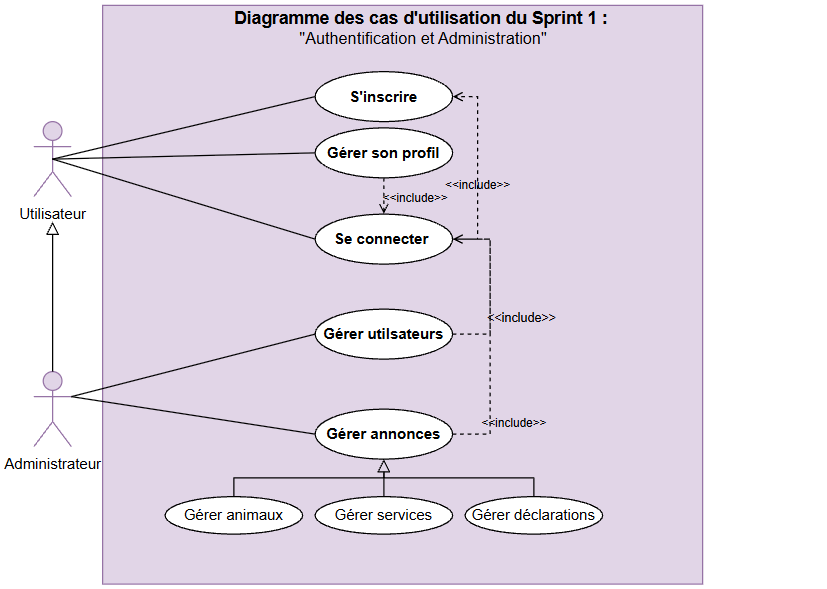
\includegraphics[width=9\linewidth, height=15.5cm, keepaspectratio]{images/use case sprint 1.png}
    \caption{Diagramme des cas d’utilisation du sprint 1}
    \label{fig:usecase-sprint1}
\end{figure}



\subsection{Descriptions textuelles des cas d’utilisation du sprint 1}


\subsubsection{Description textuelle du cas d’utilisation « S’inscrire »} 
La table \ref{tab:DTinscription} présente la description textuelle du cas d’utilisation "S’inscrire" : 
\newpage  
\begin{longtable}{|c|p{11cm}|}
\caption{Description textuelle du cas d’utilisation "S’inscrire"}
\label{tab:DTinscription} \\
\hline
\cellcolor{coloranihub} \textbf{Nom du cas d'utilisation } & S’inscrire \\
\hline
\cellcolor{coloranihub} \textbf{Acteurs} & Utilisateur \\
\hline
\cellcolor{coloranihub} \textbf{Description } & Il  s’inscrit sur AniHub afin d’accéder aux fonctionnalités. \\
\hline
\cellcolor{coloranihub} \textbf{Pré-condition } & L’utilisateur doit accéder à la page d’inscription. \\
\hline
\cellcolor{coloranihub} \textbf{Post-condition } & Un compte utilisateur est créé avec succès . \\
\hline
\cellcolor{coloranihub} \textbf{Scénario nominal } & 
\begin{enumerate}
\item L’utilisateur accède à la page d’inscription.
\item L’utilisateur saisit ses informations personnelles (nom, email, mot de passe, etc.) et valide .
\item Le système vérifie la validité des données saisies.
\item Le système crée un nouveau compte utilisateur.
\item Le système confirme la création du compte.
\item L’utilisateur est redirigé vers la page de connexion
\end{enumerate} \\
\hline
\end{longtable}


\subsubsection{Description textuelle du cas d’utilisation « Se connecter »} 
La table \ref{tab:connexion} présente la description textuelle du cas d’utilisation "Se connecter" :
\begin{longtable}{|c|p{11cm}|}
\caption{Description textuelle du cas d’utilisation "Se connecter"}
\label{tab:connexion} \\
\hline
\cellcolor{coloranihub} \textbf{Nom du cas d'utilisation } & Se connecter \\
\hline
\cellcolor{coloranihub} \textbf{Acteurs} & Utilisateur \\
\hline
\cellcolor{coloranihub} \textbf{Description } & Tout utilisateur disposant d’un compte peut s’authentifier . \\
\hline
\cellcolor{coloranihub} \textbf{Pré-condition } & L’utilisateur doit posséder un compte . \\
\hline
\cellcolor{coloranihub} \textbf{Post-condition } & il est authentifié et redirigé vers l’interface principale. \\
\hline
\cellcolor{coloranihub} \textbf{Scénario nominal } & 
\begin{enumerate}
\item L’utilisateur accède à la page de connexion.
\item Le système affiche le formulaire d’authentification.
\item L’utilisateur saisit son email et son mot de passe.
\item L’utilisateur valide le formulaire de connexion.
\item Le système vérifie les informations d’identification.
\item Le système authentifie l’utilisateur.
\item Le système redirige l’utilisateur vers la page d’accueil.
\end{enumerate} \\
\hline
\end{longtable}



\newpage


\newpage 

\subsubsection{Description textuelle du cas d’utilisation « Gérer son profil »}
La table \ref{tab:gerer_profil} présente la description textuelle du cas d’utilisation "Gérer son profil" :
\begin{longtable}{|c|p{11cm}|}
\caption{Description textuelle du cas d'utilisation "Gérer son profil"}
\label{tab:gerer_profil} \\
\hline
\cellcolor{coloranihub}\textbf{Nom du cas d'utilisation } & Gérer son profil (modifier / supprimer) \\
\hline
\cellcolor{coloranihub}\textbf{Acteurs} & Utilisateur \\
\hline
\cellcolor{coloranihub}\textbf{Description } & L’utilisateur peut consulter, modifier ou supprimer son profil. \\
\hline
\cellcolor{coloranihub}\textbf{Pré-condition } & L’utilisateur doit être authentifié. \\
\hline
\cellcolor{coloranihub}\textbf{Post-condition } & Les informations du profil sont mises à jour ou le compte est supprimé avec succès. \\
\hline

\cellcolor{coloranihub}\textbf{Scénario nominal } &
\begin{enumerate}
\item L’utilisateur accède à la page d’accueil d’AniHub.
\item L’utilisateur sélectionne « Mon espace » dans la barre de navigation.
\item Le système redirige l’utilisateur vers son profil.
\item Le système affiche les informations personnelles de l’utilisateur.
\item L’utilisateur choisit une action.
\item Cas modification :
\begin{itemize}
\item L’utilisateur clique sur « Modifier profil ».
\item Le système affiche le formulaire pré-rempli.
\item L’utilisateur modifie ses informations.
\item L’utilisateur valide les modifications.
\item Le système vérifie et enregistre les nouvelles données. 
\item le système affiche un message confirmant la mise à jour des informations avec succès . 
\end{itemize}
\item Cas suppression :
\begin{itemize}
\item L’utilisateur clique sur « Supprimer mon compte ».
\item Le système demande une confirmation.
\item L’utilisateur confirme la suppression.
\item Le système supprime définitivement le compte et le redirige vers la page d’inscription..
\end{itemize}
\end{enumerate} \\
\hline

\cellcolor{coloranihub}\textbf{Scénario alternatif :} &
\begin{itemize}
\item Erreur lors de la modification : le système affiche un message d’erreur.
\item Annulation de la suppression : e compte de l’utilisateur est conservé.
\end{itemize} \\
\hline

\end{longtable}






\newpage 

\subsubsection{Description textuelle du cas d’utilisation « Gérer les utilisateurs »}
La table \ref{tab:gerer_utilisateurs} présente la description textuelle du cas d’utilisation "Gérer les utilisateurs" :
\begin{longtable}{|c|p{11cm}|}
\caption{Description textuelle du cas d'utilisation "Gérer les utilisateurs"}
\label{tab:gerer_utilisateurs} \\
\hline
\cellcolor{coloranihub}\textbf{Nom du cas d'utilisation } & Gérer les utilisateurs \\
\hline
\cellcolor{coloranihub}\textbf{Acteurs} & Administrateur \\
\hline
\cellcolor{coloranihub}\textbf{Description } & L’administrateur peut gérer les comptes utilisateurs (consultation, modification, suppression). \\
\hline
\cellcolor{coloranihub}\textbf{Pré-condition } & L’administrateur doit être authentifié. \\
\hline
\cellcolor{coloranihub}\textbf{Post-condition } & Les données de l’utilisateur sont mises à jour ou supprimées avec succès. \\
\hline

\cellcolor{coloranihub}\textbf{Scénario nominal } &
\begin{enumerate}
\item L’administrateur accède à la page d’accueil d’AniHub.
\item L’administrateur accède à son espace administrateur.
\item Le système affiche le tableau de bord administrateur.
\item L’administrateur consulte le tableau de bord pour voir les statistiques des utilisateurs.
\item L’administrateur accède ensuite à la section « Gestion des utilisateurs ».
\item Le système affiche la liste des utilisateurs.
\item L’administrateur sélectionne un utilisateur.

\item Cas modification :
\begin{itemize}
\item L’administrateur clique sur « Modifier ».
\item Le système affiche le formulaire de modification.
\item L’administrateur met à jour ses informations.
\item Le système enregistre les modifications.
\end{itemize}

\item Cas suppression :
\begin{itemize}
\item L’administrateur clique sur « Supprimer ».
\item Le système demande une confirmation.
\item L’administrateur confirme la suppression.
\item Le système supprime définitivement le compte utilisateur.
\end{itemize}

\item Le système affiche un message de confirmation .
\end{enumerate} \\
\hline

\cellcolor{coloranihub}\textbf{Scénario alternatif :} &
\begin{itemize}
\item Annulation de la suppression : aucune action n’est effectuée et le compte est conservé.
\item Erreur lors de la modification : le système affiche un message d’erreur.
\end{itemize} \\
\hline
\end{longtable} 
\newpage 



\subsubsection{Description textuelle du cas d’utilisation « Gérer les annonces »}
La table \ref{tab:gerer_annonces_admin} présente la description textuelle du cas d’utilisation "Gérer les annonces" :

\begin{longtable}{|c|p{11cm}|}
\caption{Description textuelle du cas d'utilisation "Gérer les annonces"}
\label{tab:gerer_annonces_admin} \\
\hline
\cellcolor{coloranihub}\textbf{Nom du cas d'utilisation } & Gérer les annonces \\
\hline
\cellcolor{coloranihub}\textbf{Acteurs} & Administrateur \\
\hline
\cellcolor{coloranihub}\textbf{Description } & L’administrateur peut consulter et gérer les différentes annonces de la plateforme .\\
\hline
\cellcolor{coloranihub}\textbf{Pré-condition } & L’administrateur doit être authentifié. \\
\hline
\cellcolor{coloranihub}\textbf{Post-condition } & Les annonces supprimées ne sont plus visibles sur la plateforme. \\
\hline

\cellcolor{coloranihub}\textbf{Scénario nominal } &
\begin{enumerate}
\item L’administrateur accède à la page d’accueil d’AniHub.
\item L’administrateur se connecte à son espace administrateur.
\item Le système affiche le tableau de bord administrateur avec des statistiques générales.
\item L’administrateur accède à la section « Gestion des annonces ».
\item Le système affiche les différents types d’annonces disponibles.
\item L’administrateur choisit un type d’annonce (adoption, accouplement, vente, déclaration ou service).
\item Le système affiche la liste des annonces correspondant au type sélectionné.

\item Cas suppression :
\begin{itemize}
\item L’administrateur sélectionne une annonce.
\item L’administrateur clique sur « Supprimer ».
\item Le système demande une confirmation.
\item L’administrateur confirme la suppression.
\item Le système supprime définitivement l’annonce.
\end{itemize}

\item Le système affiche un message de confirmation de l’opération.
\end{enumerate} \\
\hline

\cellcolor{coloranihub}\textbf{Scénario alternatif :} &
\begin{itemize}
\item Annulation de la suppression : aucune action n’est effectuée et l’annonce est conservée.
\item Erreur lors de la suppression : le système affiche un message d’erreur.
\end{itemize} \\
\hline

\end{longtable}
\newpage 
 
\subsection{Diagrammes des classes du sprint 1}  
Dans cette section, nous présentons le diagramme de classes du Sprint 1, qui regroupe l’ensemble des classes liées à l’authentification et à l’administration.

La figure \ref{fig:class_diagram_sprint1} illustre le diagramme de classes correspondant : 
\begin{figure}[H]
    \centering
    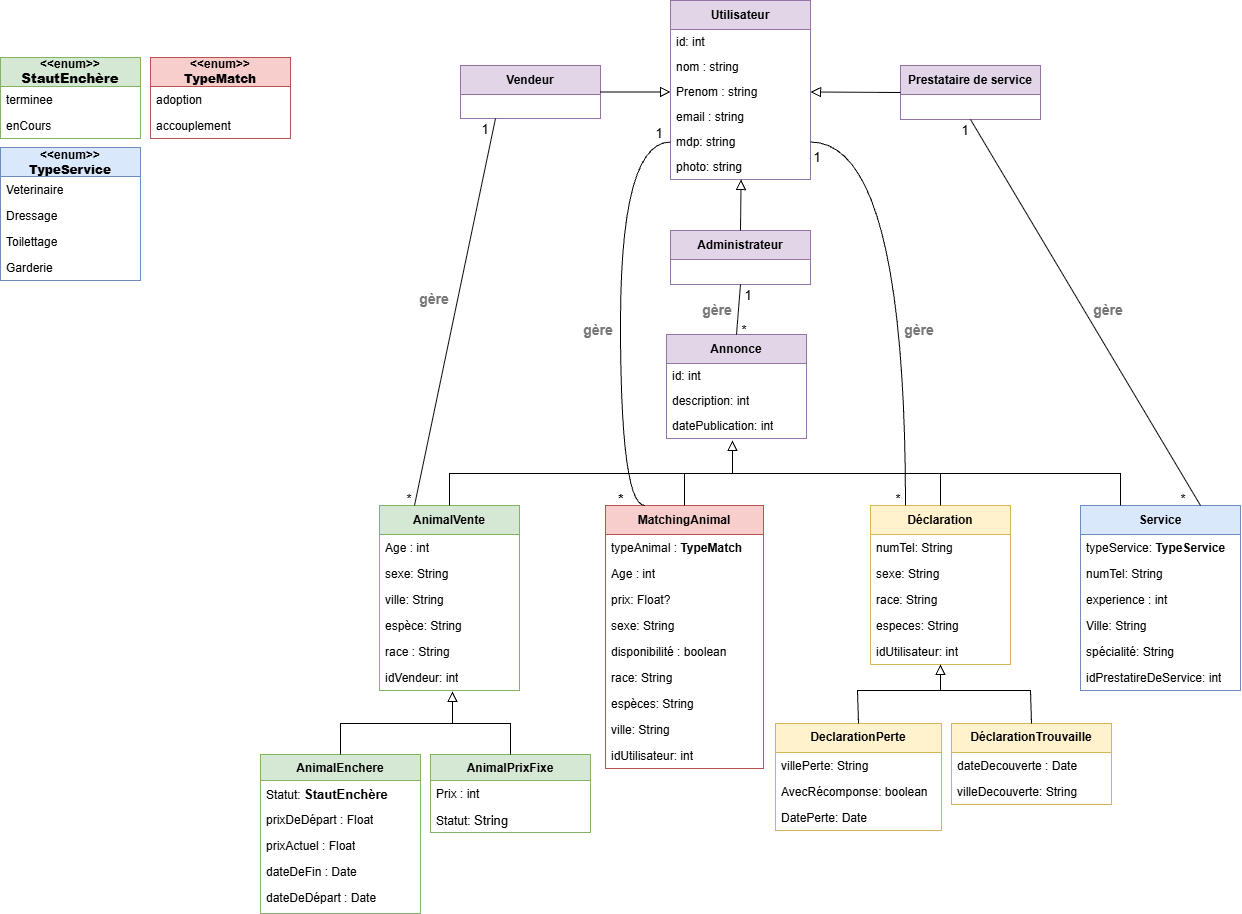
\includegraphics[width=1\textwidth, height=20cm, keepaspectratio]{images/class diagram sprint 1.png}
    \caption{Diagramme de classes du sprint 1}
    \label{fig:class_diagram_sprint1}
\end{figure} 

\subsection{Diagrammes de séquences du sprint 1}

Cette section présente les diagrammes de séquences du premier sprint, illustrant les interactions entre les différents composants du système.

\subsubsection{Diagramme de séquence : inscription}
La figure \ref{fig:sequence-inscription} illustre les interactions entre l’utilisateur et le système lors du processus d’inscription :  
\newpage
\begin{figure}[H]
\centering
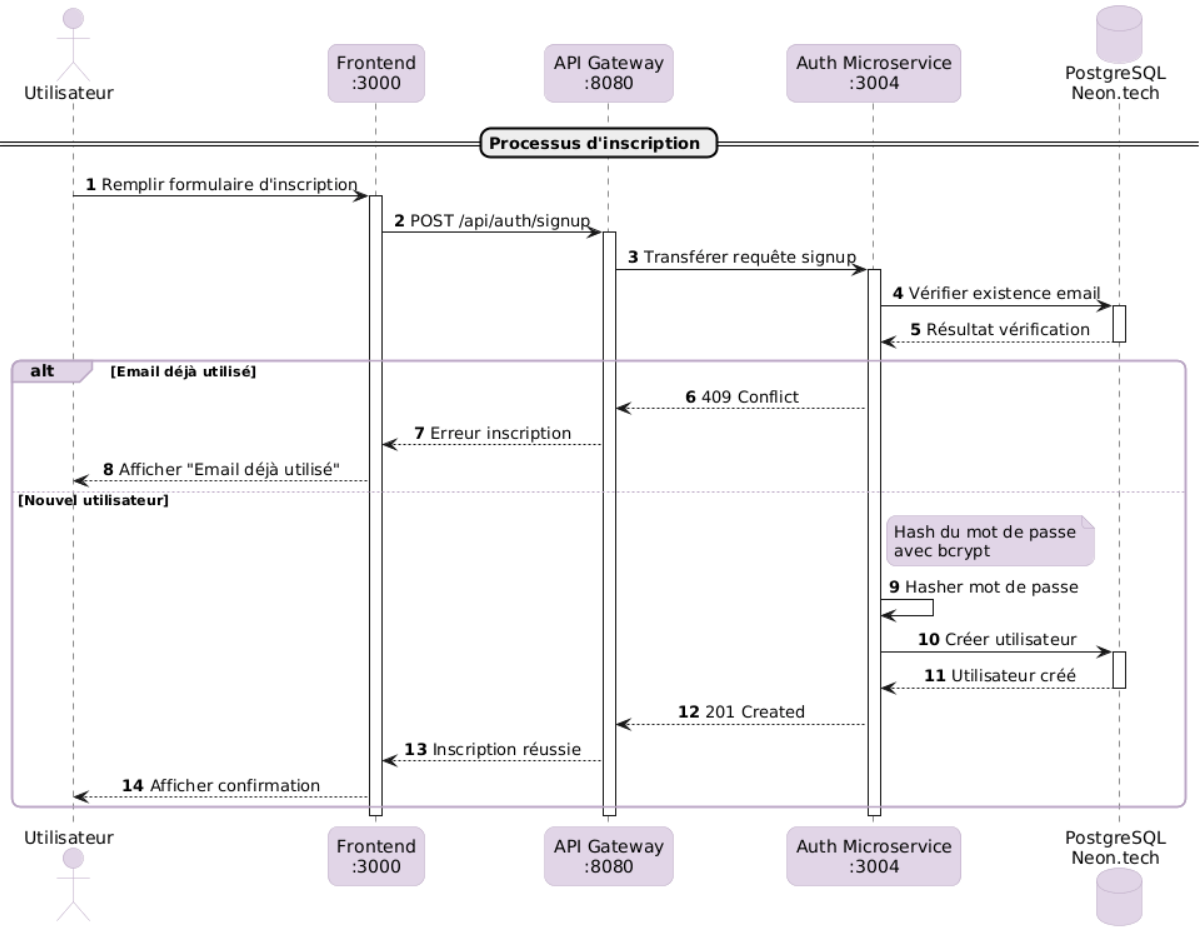
\includegraphics[width=0.6\textwidth]{images/sinscrire.png}
\caption{Diagramme de séquence de l’inscription}
\label{fig:sequence-inscription}
\end{figure}

\vspace{-0.5cm}

\subsubsection{Diagramme de séquence : connexion}
La figure \ref{fig:sequence-connexion} illustre les interactions entre l’utilisateur et le système lors du processus de connexion : 
\begin{figure}[H]
\centering
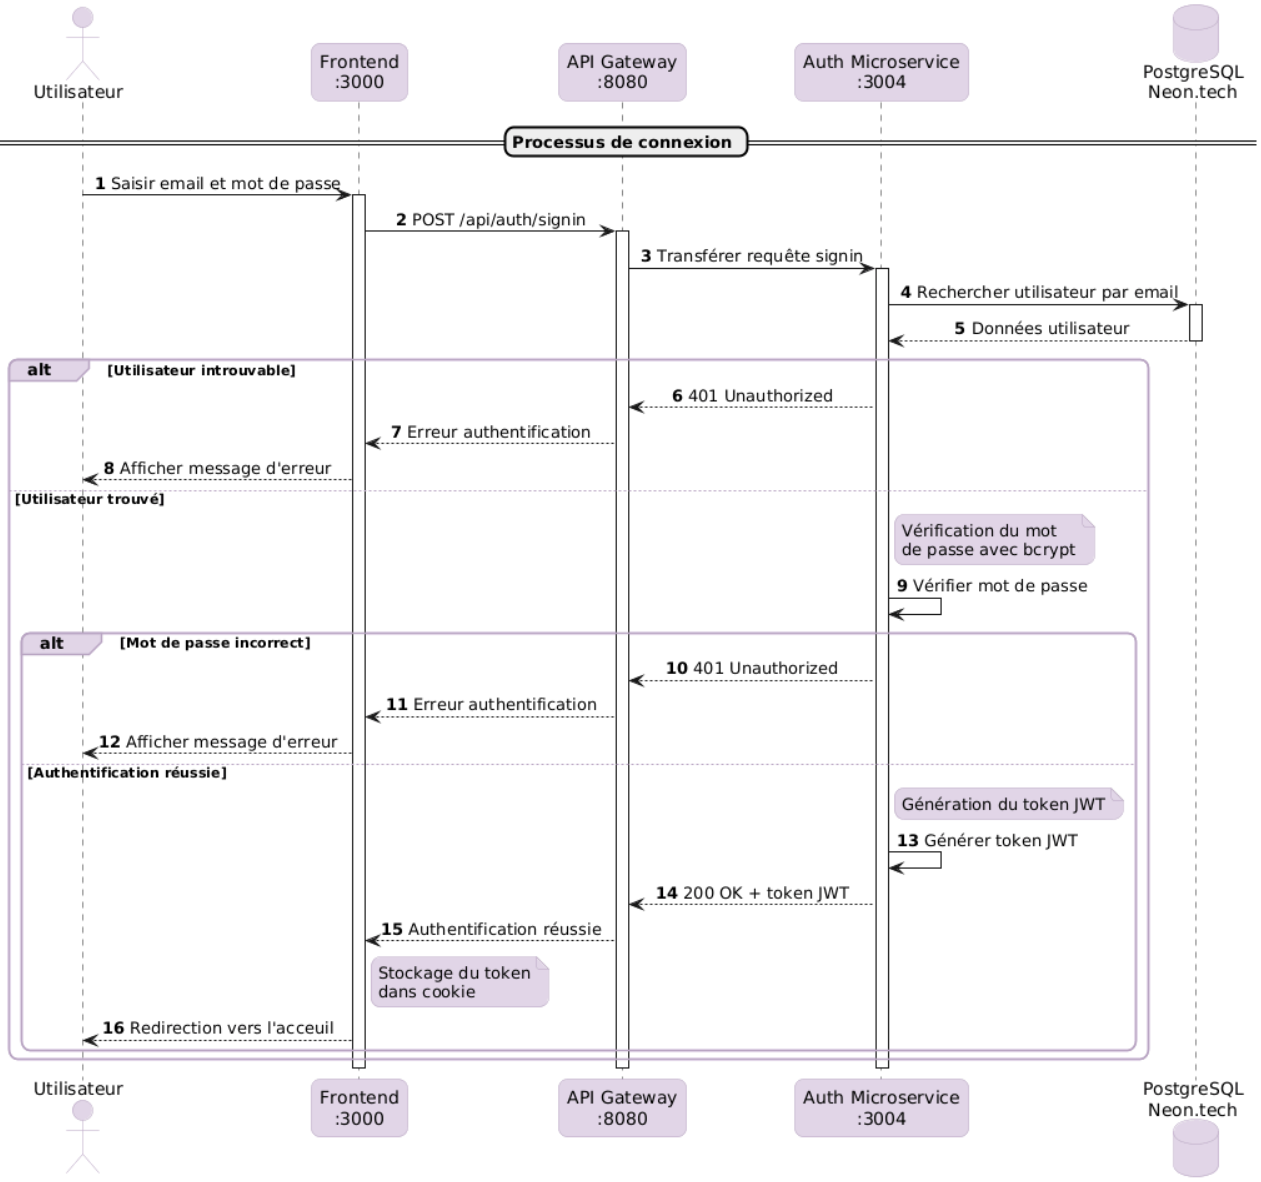
\includegraphics[width=0.6\textwidth]{images/connexion.png}
\caption{Diagramme de séquence de la connexion}
\label{fig:sequence-connexion}
\end{figure}
\newpage  
\subsubsection{Diagramme de séquence : gestion des utilisateurs}

La figure \ref{fig:sequence-gerer-users} illustre le processus de gestion des utilisateurs par l’administrateur. Elle décrit les différentes interactions entre le frontend, l’API Gateway et le microservice d’authentification, notamment lors des opérations de modification et de suppression d’un utilisateur. Le diagramme met en évidence la vérification des droits d’accès de l’administrateur ainsi que le traitement des actions autorisées ou refusées : 
\begin{figure}[H]
\centering
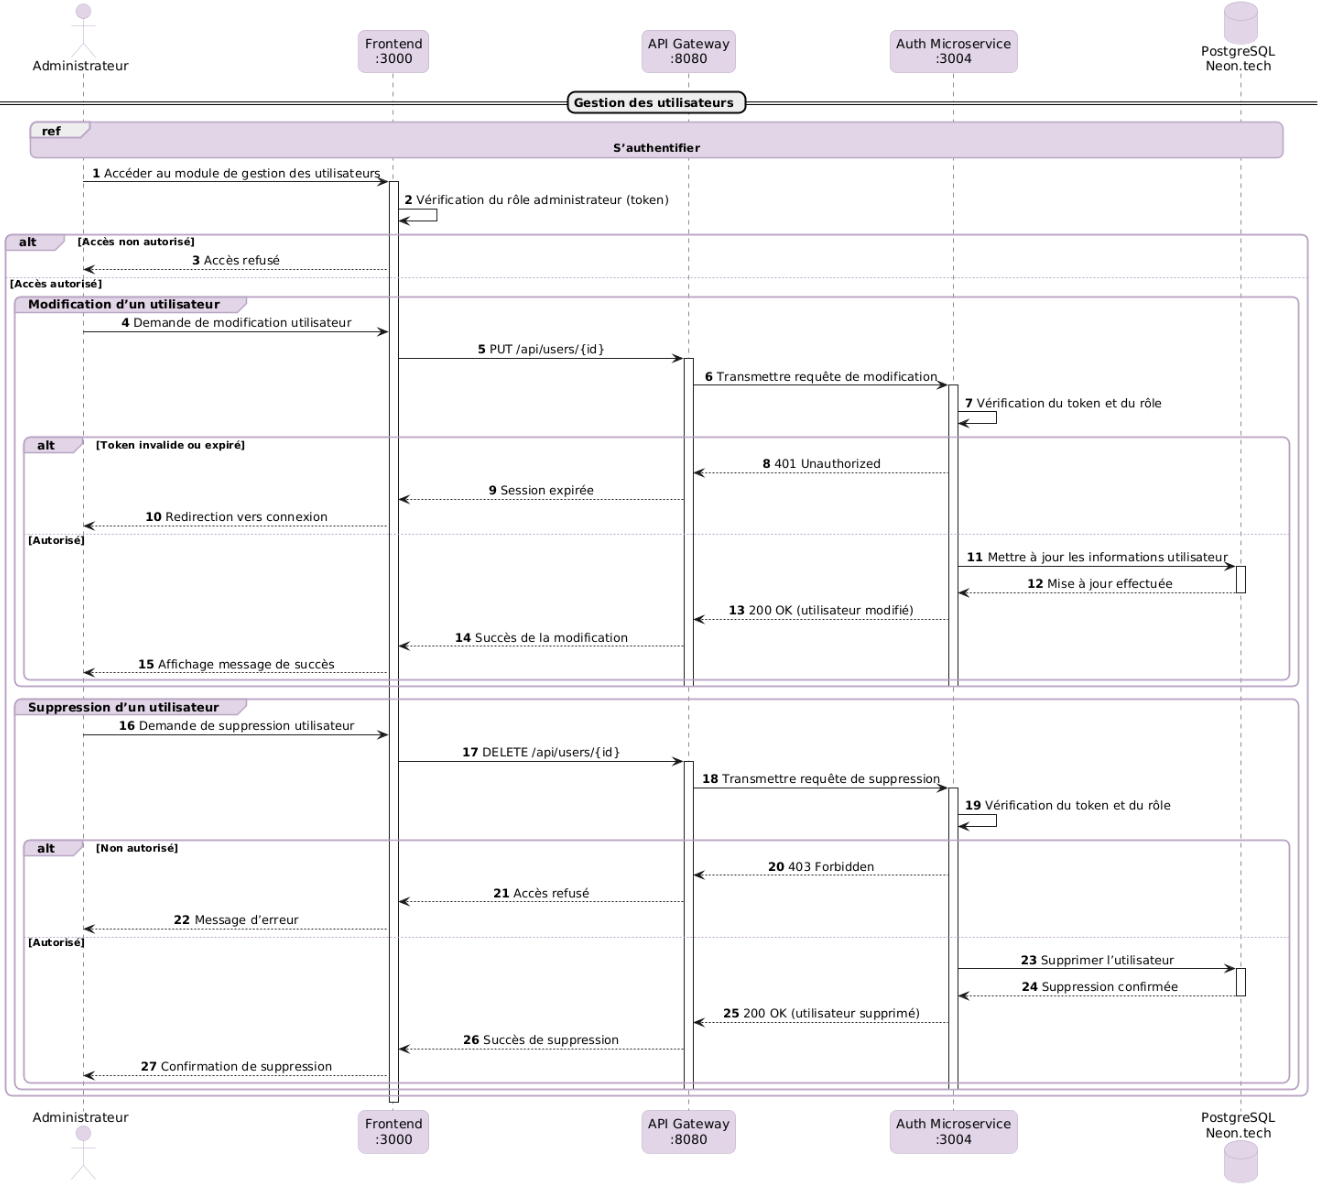
\includegraphics[width=\textwidth]{images/gererutilsateurs.png}
\caption{Diagramme de séquence de la gestion des utilisateurs}
\label{fig:sequence-gerer-users}
\end{figure} 
\newpage
\subsubsection{Diagramme de séquence : gestion des annonces} 

La figure \ref{fig:sequence-gerer-annonces} illustre le processus de gestion des annonces des modules AniMatch, AniFound, AniMarket et AniCare, incluant les opérations d’activation, de désactivation et de suppression. Elle met en évidence les interactions entre le frontend, l’API Gateway et les microservices concernés, ainsi que la publication des notifications aux utilisateurs via le service de notification : 
\begin{figure}[H]
\centering
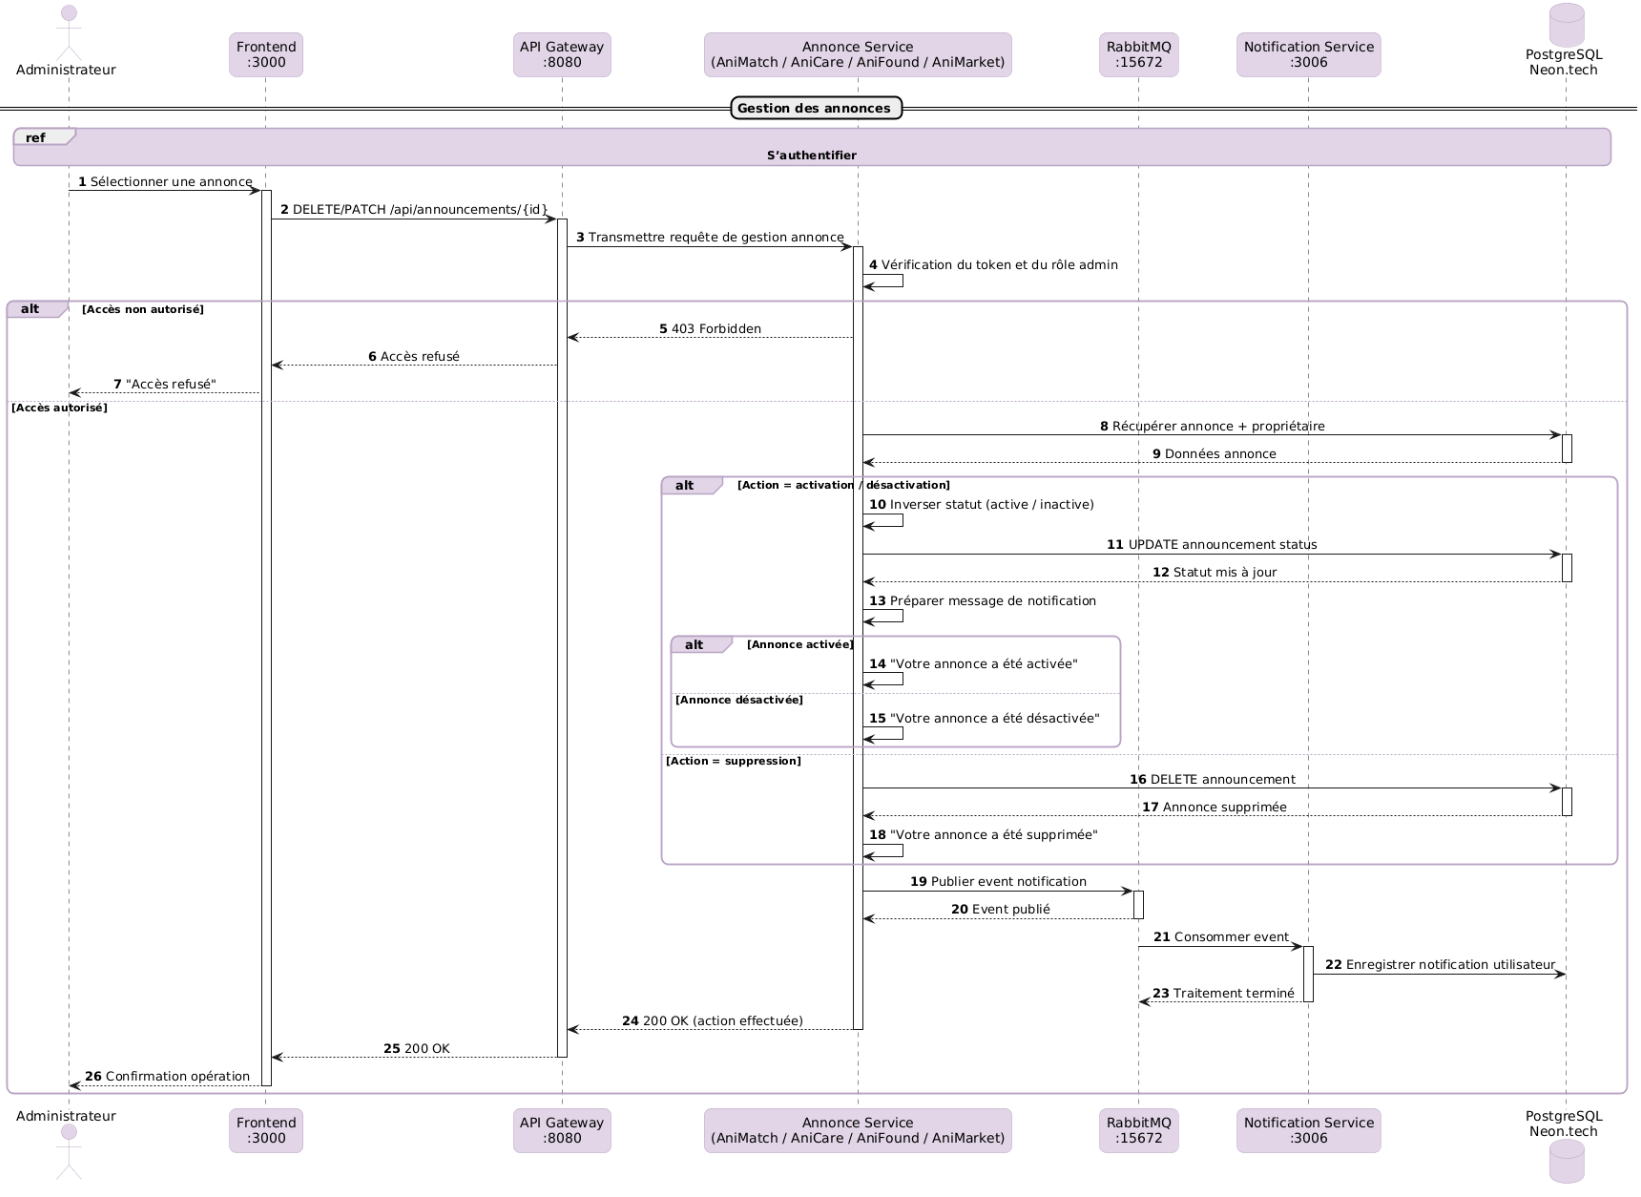
\includegraphics[width=\textwidth,height=0.99\textheight,keepaspectratio]{images/gererannonces.png}
\caption{Diagramme de séquence de la gestion des annonces}
\label{fig:sequence-gerer-annonces}
\end{figure} 
\newpage
\subsection{Réalisation su sprint 1 }  
\subsubsection{Réalisation des maquettes Figma pour les interfaces de la plateforme AniHub}

La figure \ref{fig:figma_maquettes} présente les maquettes réalisées avec Figma pour toutes les interfaces de la plateforme AniHub.

\begin{figure}[H]
    \centering
    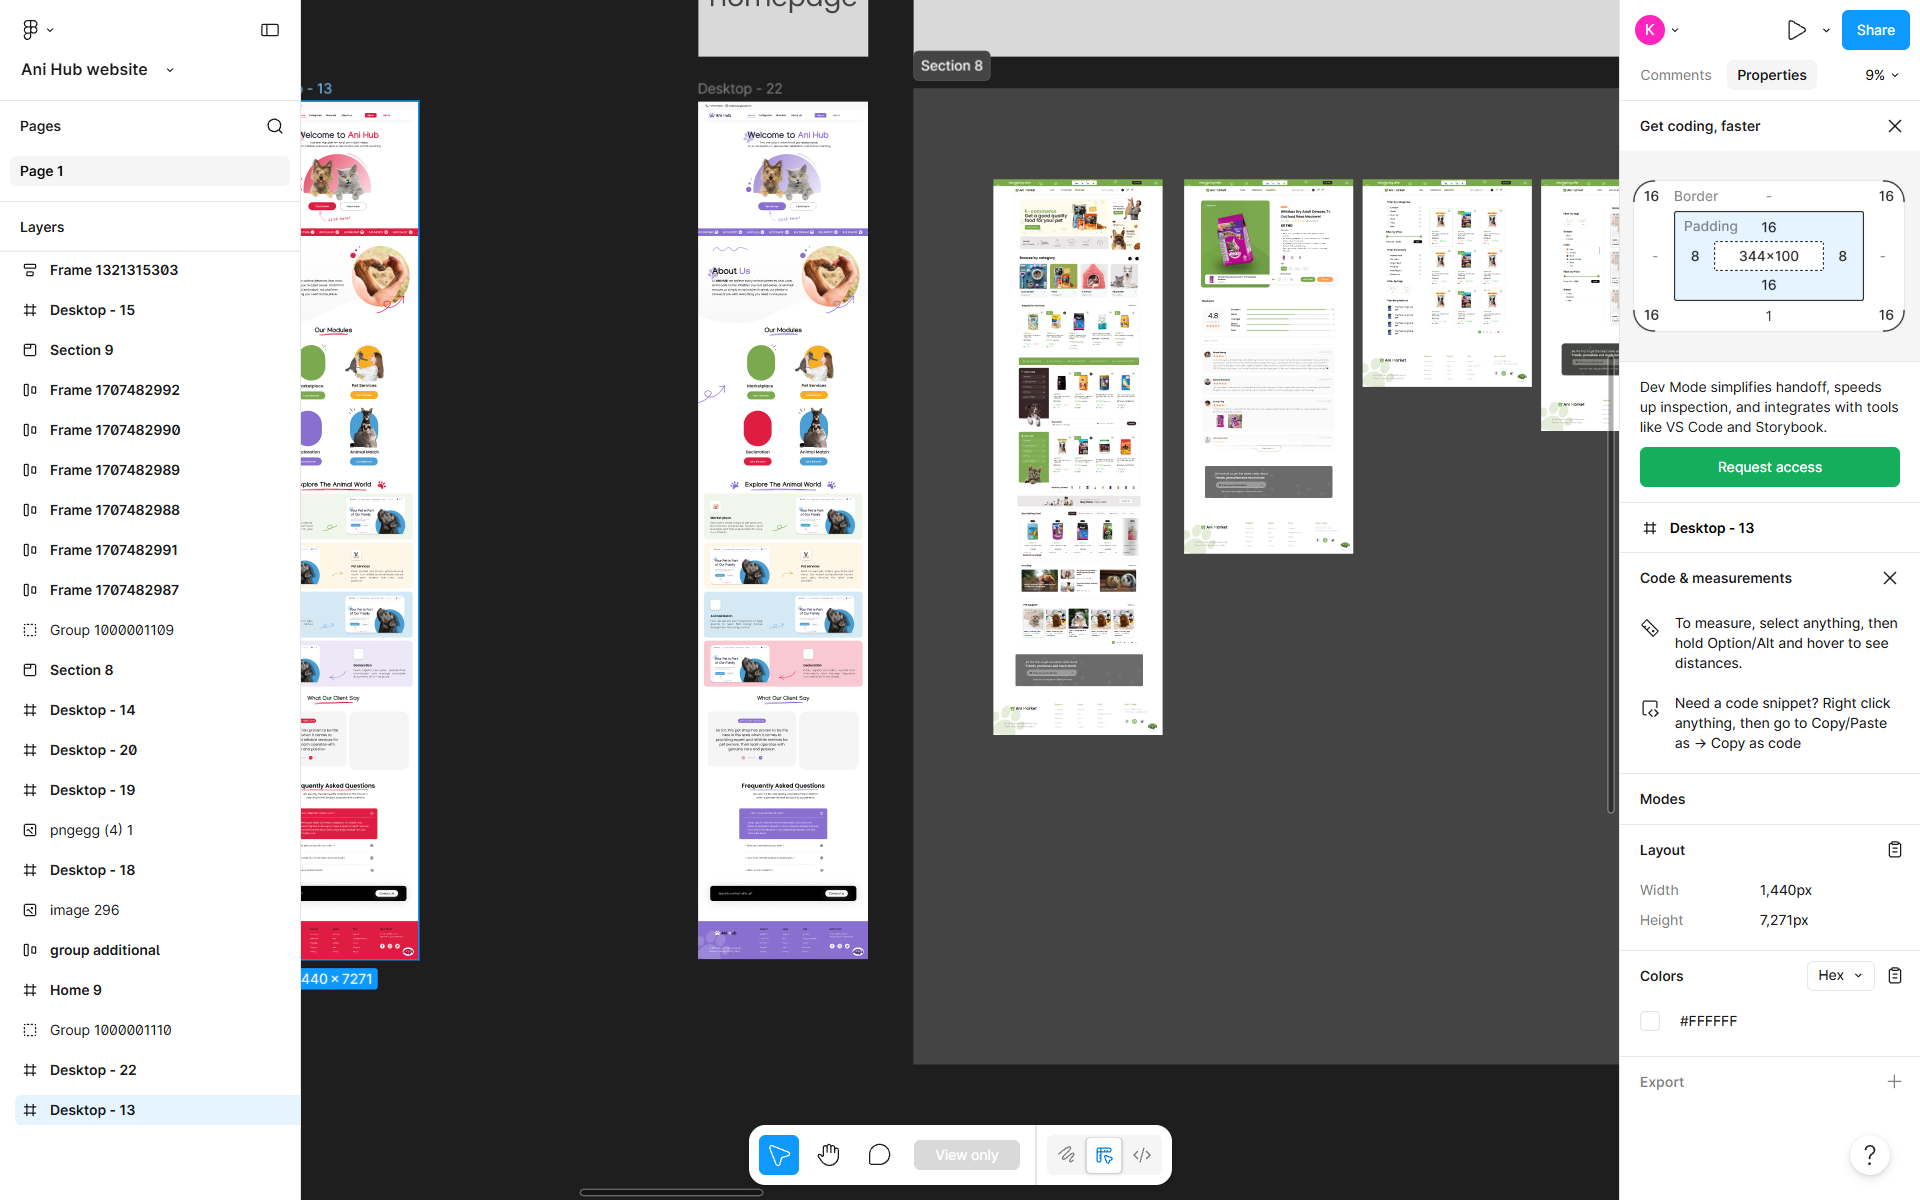
\includegraphics[width=0.64\textwidth]{images/maquettes figma.png}
    \caption{Maquettes Figma des interfaces AniHub}
    \label{fig:figma_maquettes}
\end{figure}


\subsubsection{Page d’accueil AniHub}

La figure \ref{fig:home_anihub} présente la page d’accueil de la plateforme AniHub :

\begin{figure}[h!]
    \centering
    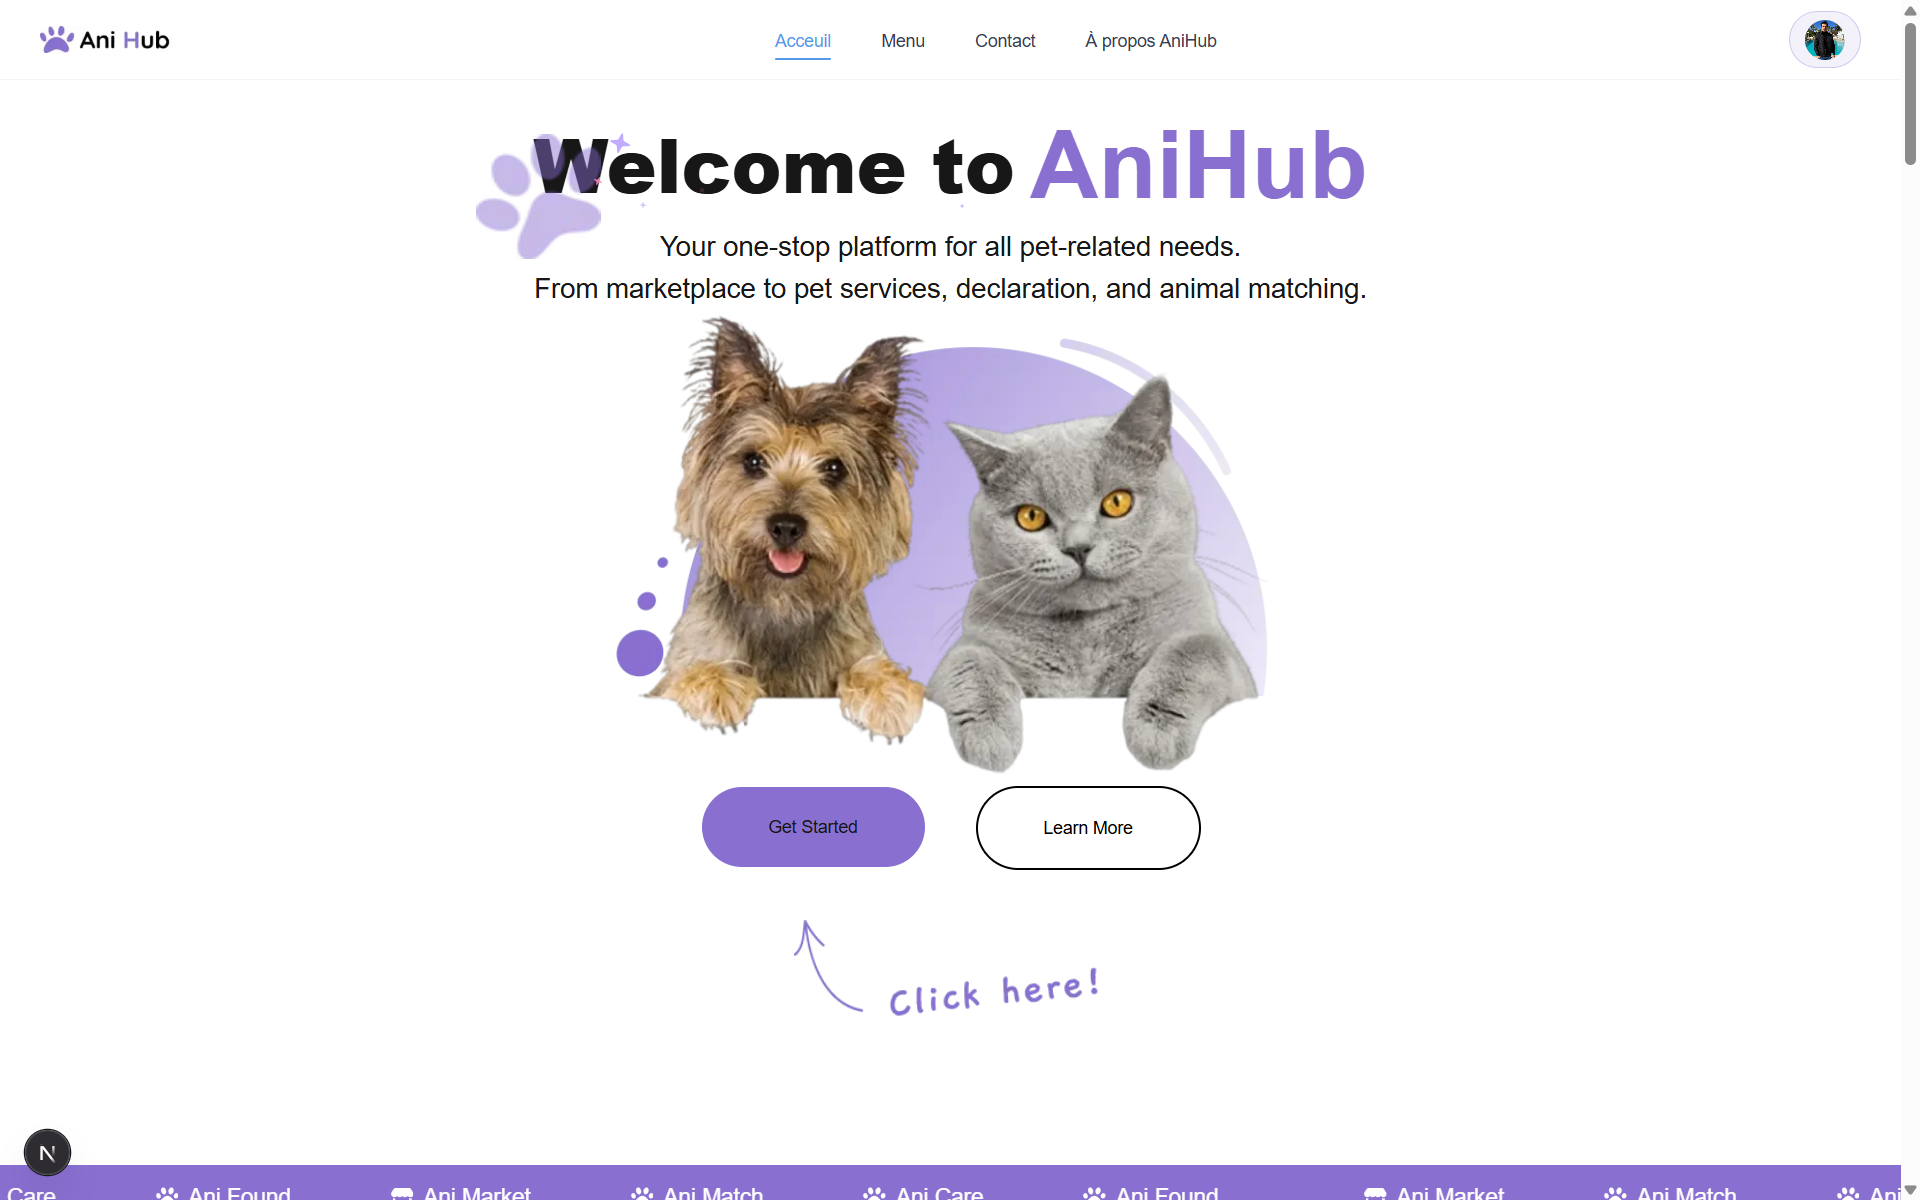
\includegraphics[width=0.72\textwidth]{images/acceuil.png}
    \caption{Page d’accueil AniHub}
    \label{fig:home_anihub}
\end{figure}

\subsubsection{Interfaces d'inscription et de connexion}

Les figures \ref{fig:signup_anihub} et \ref{fig:signin_anihub} illustrent les interfaces d’inscription et de connexion de la plateforme AniHub, qui permettent respectivement la création de compte et l’authentification des utilisateurs : 
\begin{figure}[h!]
    \centering

    \begin{minipage}{0.48\textwidth}
        \centering
        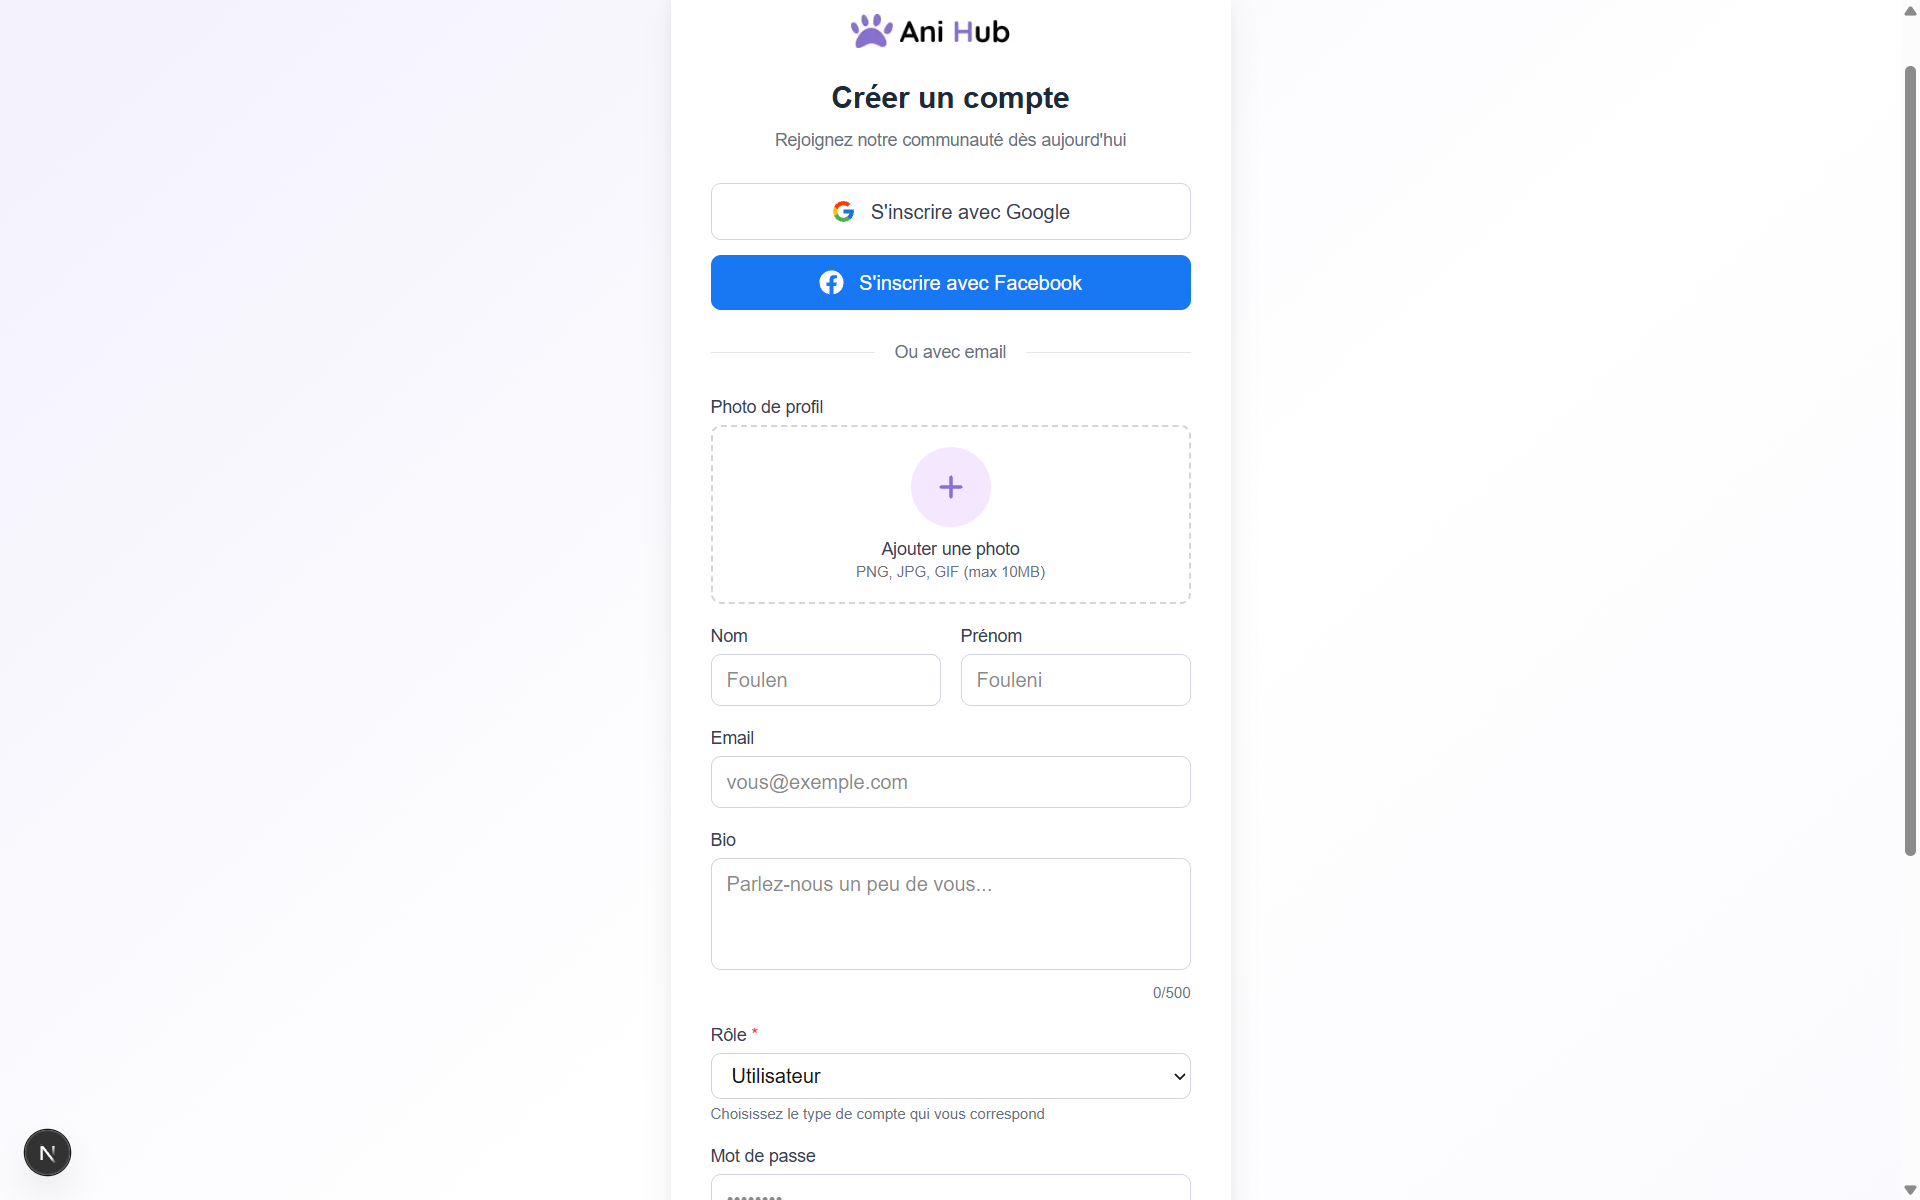
\includegraphics[width=\textwidth]{images/sign up .png}
        \caption{Interface d'inscription AniHub}
        \label{fig:signup_anihub}
    \end{minipage}
    \hfill
    \begin{minipage}{0.48\textwidth}
        \centering
        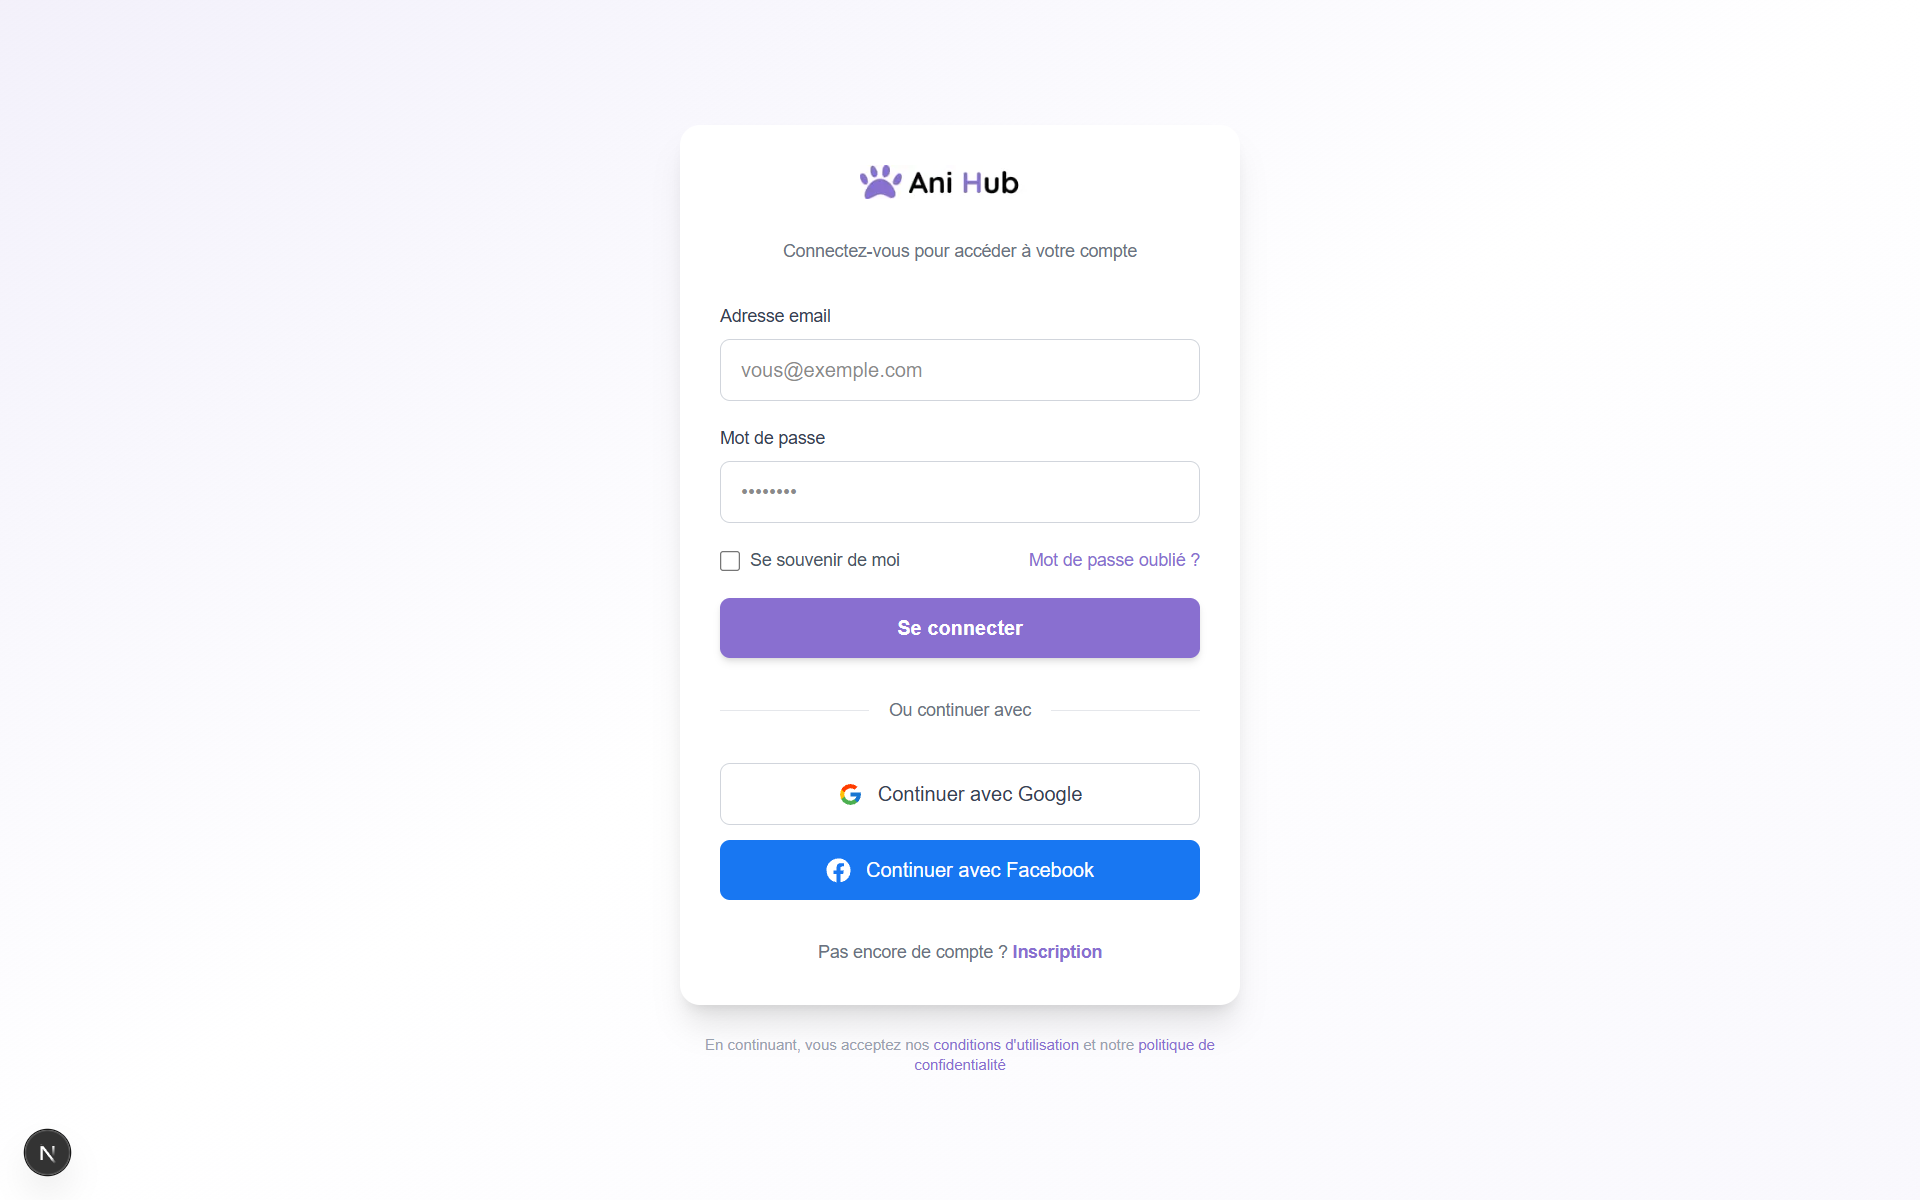
\includegraphics[width=\textwidth]{images/sign in.png}
        \caption{Interface de connexion AniHub}
        \label{fig:signin_anihub}
    \end{minipage}

\end{figure}

\subsubsection{Interface du profil utilisateur}

La figure \ref{fig:profile_anihub} présente l’interface du profil utilisateur AniHub, qui permet à l’utilisateur de consulter et de gérer ses informations personnelles : 
\begin{figure}[H]
    \centering
    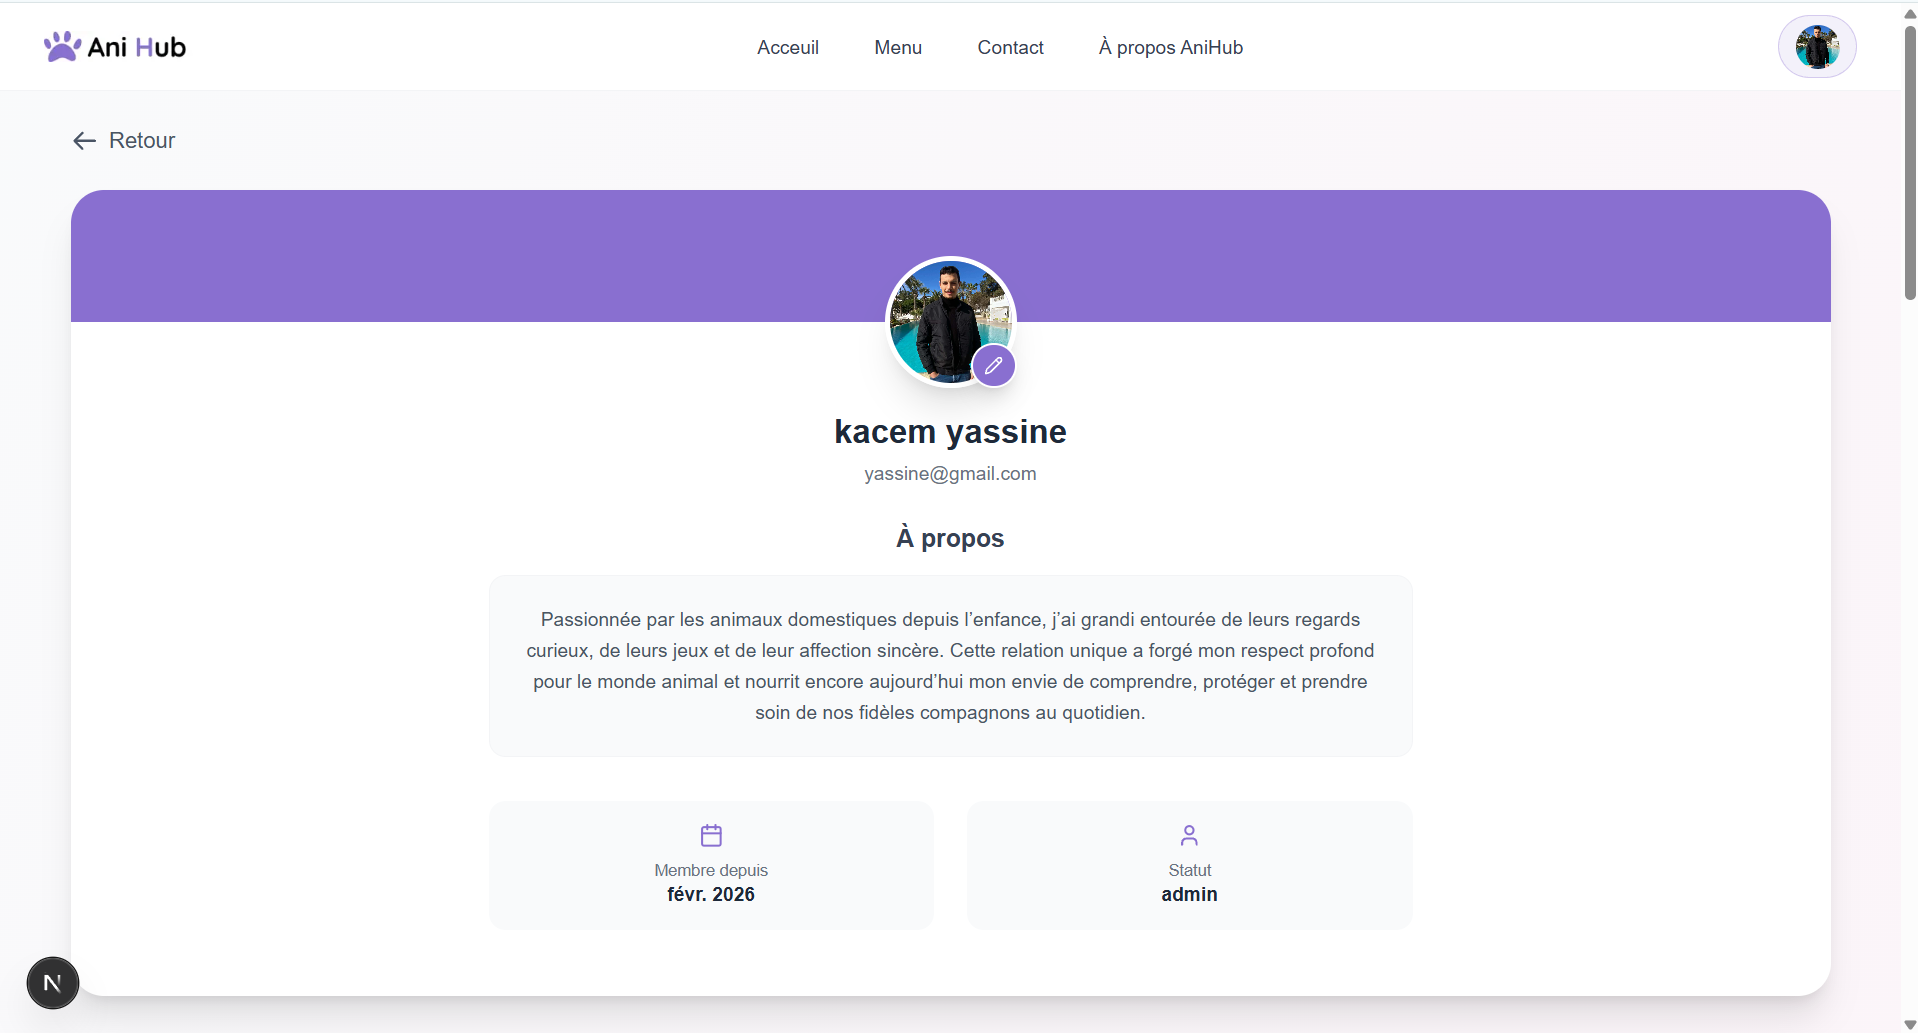
\includegraphics[width=\textwidth]{images/gestion profil.png}
    \caption{Interface du profil utilisateur AniHub}
    \label{fig:profile_anihub}
\end{figure}

\newpage 

\subsubsection{Interface du tableau de bord administrateur}

La figure \ref{fig:admin_dashboard} présente l’accueil du tableau de bord administrateur de la plateforme AniHub, qui affiche des statistiques globales sur la plateforme : 
\begin{figure}[H]
    \centering
    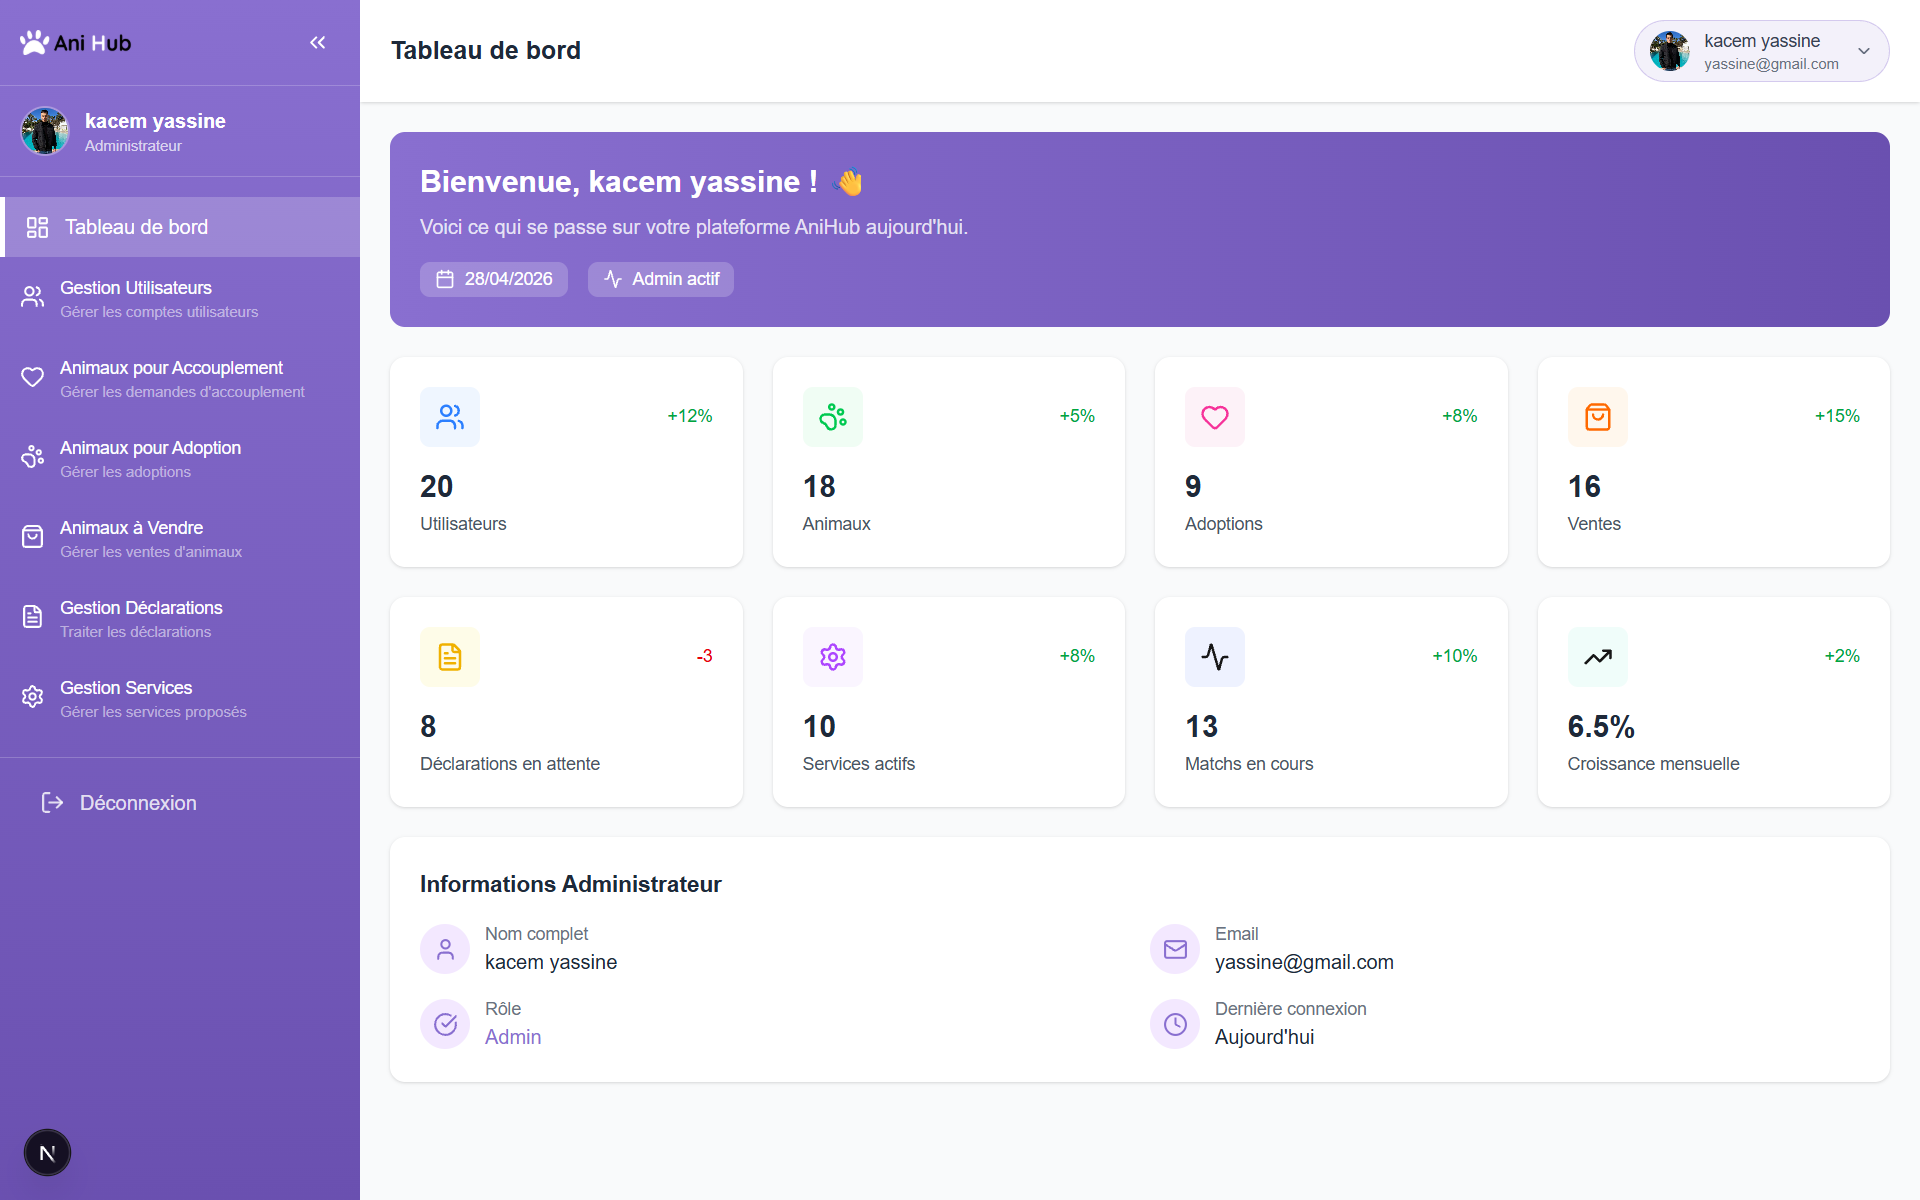
\includegraphics[width=0.75\textwidth]{images/dashboard stats.png}
    \caption{Tableau de bord administrateur AniHub}
    \label{fig:admin_dashboard}
\end{figure}

\subsubsection{Interface de gestion des utilisateurs}

La figure \ref{fig:user_management} présente l’interface de gestion des utilisateurs de la plateforme AniHub : 

\begin{figure}[H]
    \centering
    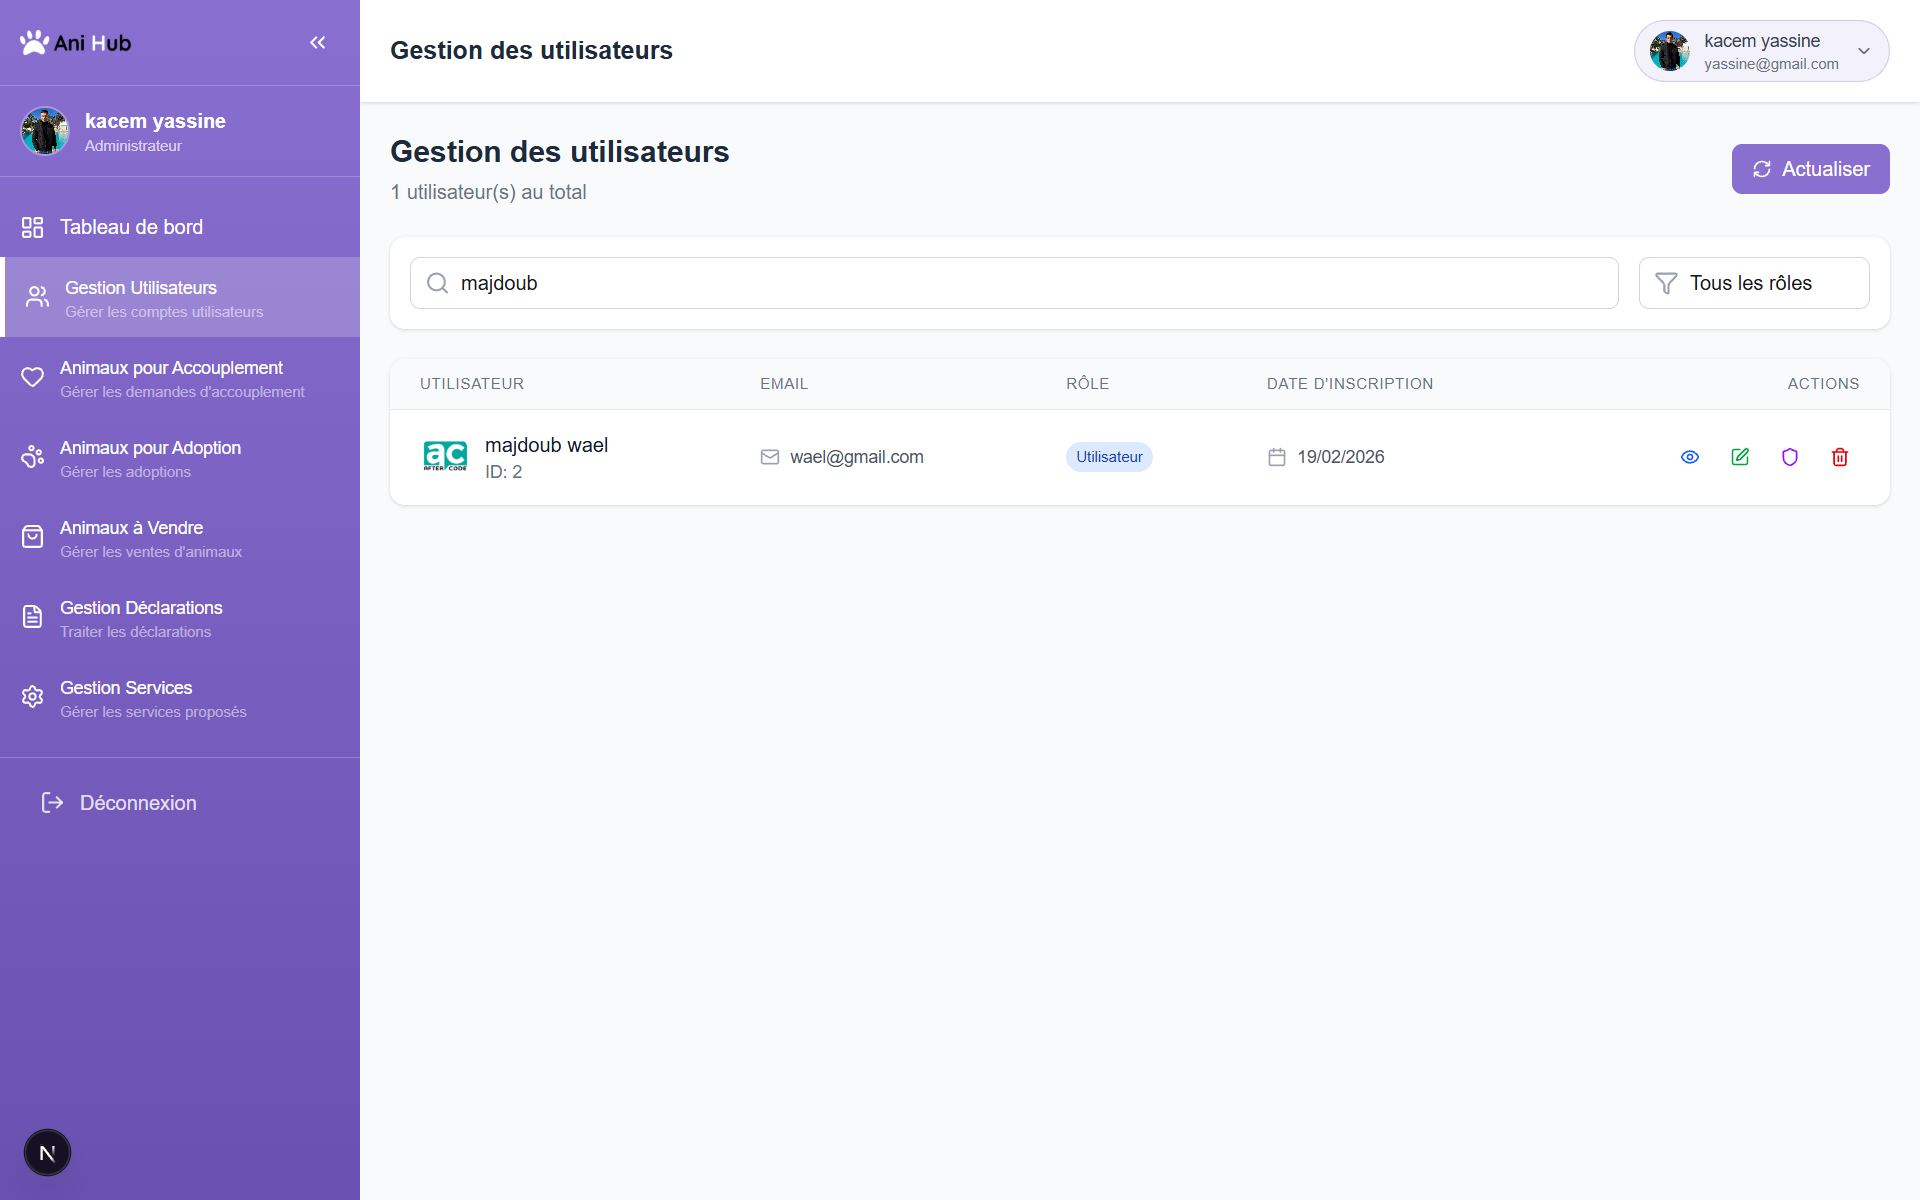
\includegraphics[width=0.78\textwidth]{images/gestion utilsateurs.png}
    \caption{Interface de gestion des utilisateurs AniHub}
    \label{fig:user_management}
\end{figure}

\newpage

\subsubsection{Interfaces d’administration pour le module AniMatch avec statistiques} 

Les figures \ref{fig:animatch_manage} et \ref{fig:animatch_stats} illustrent les interfaces permettant à l’administrateur de gérer le module AniMatch (accouplement et adoption ) et de consulter les statistiques associées, notamment le suivi des demandes de mise en relation, leur validation ainsi que l’analyse de l’activité des utilisateurs au sein de ce module : 
\begin{figure}[h!]
    \centering
    
    \begin{minipage}{0.48\textwidth}
        \centering
        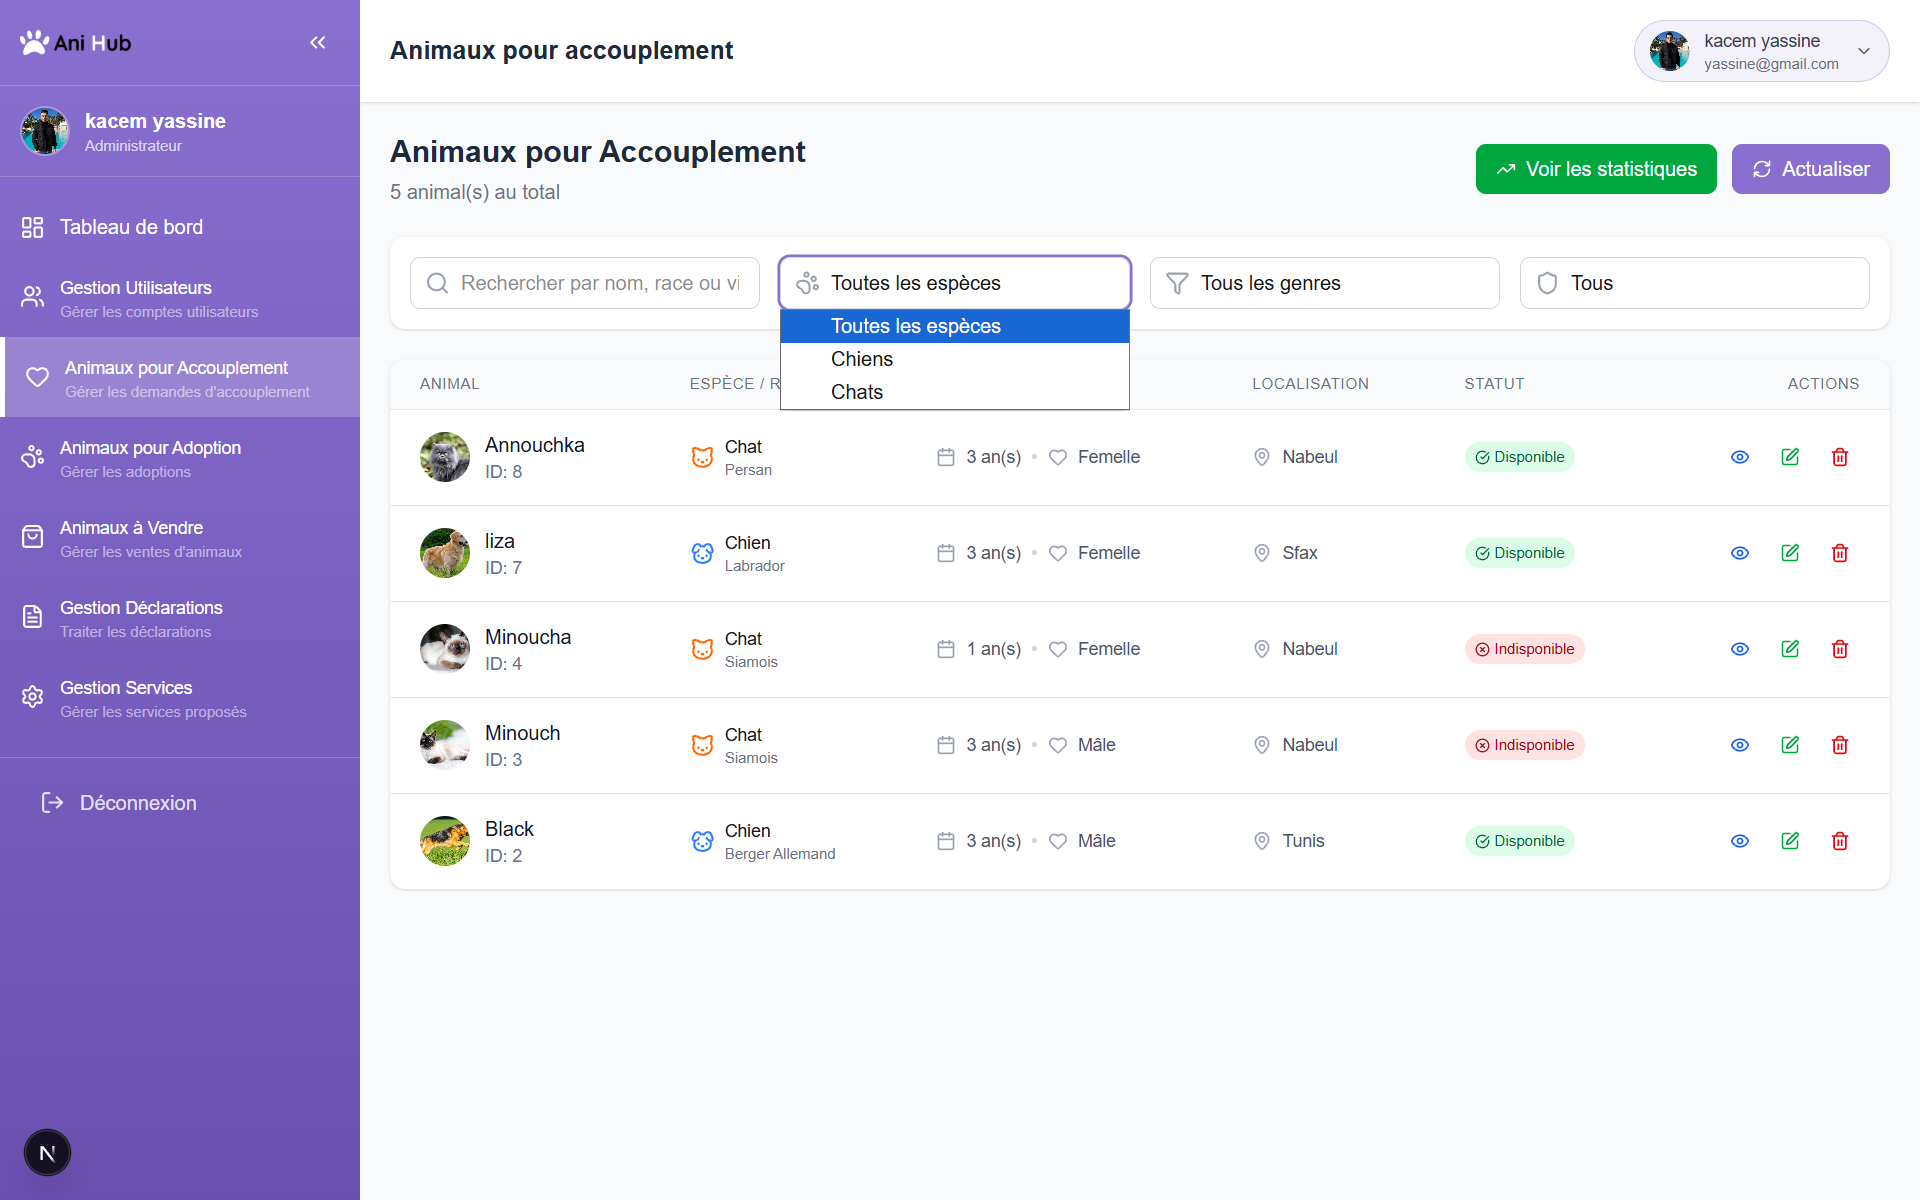
\includegraphics[width=\textwidth]{images/dashboard animatch 1.png}
        \caption{Interface d’administration de gestion d’AniMatch}
        \label{fig:animatch_manage}
    \end{minipage}
    \hfill
    \begin{minipage}{0.48\textwidth}
        \centering
        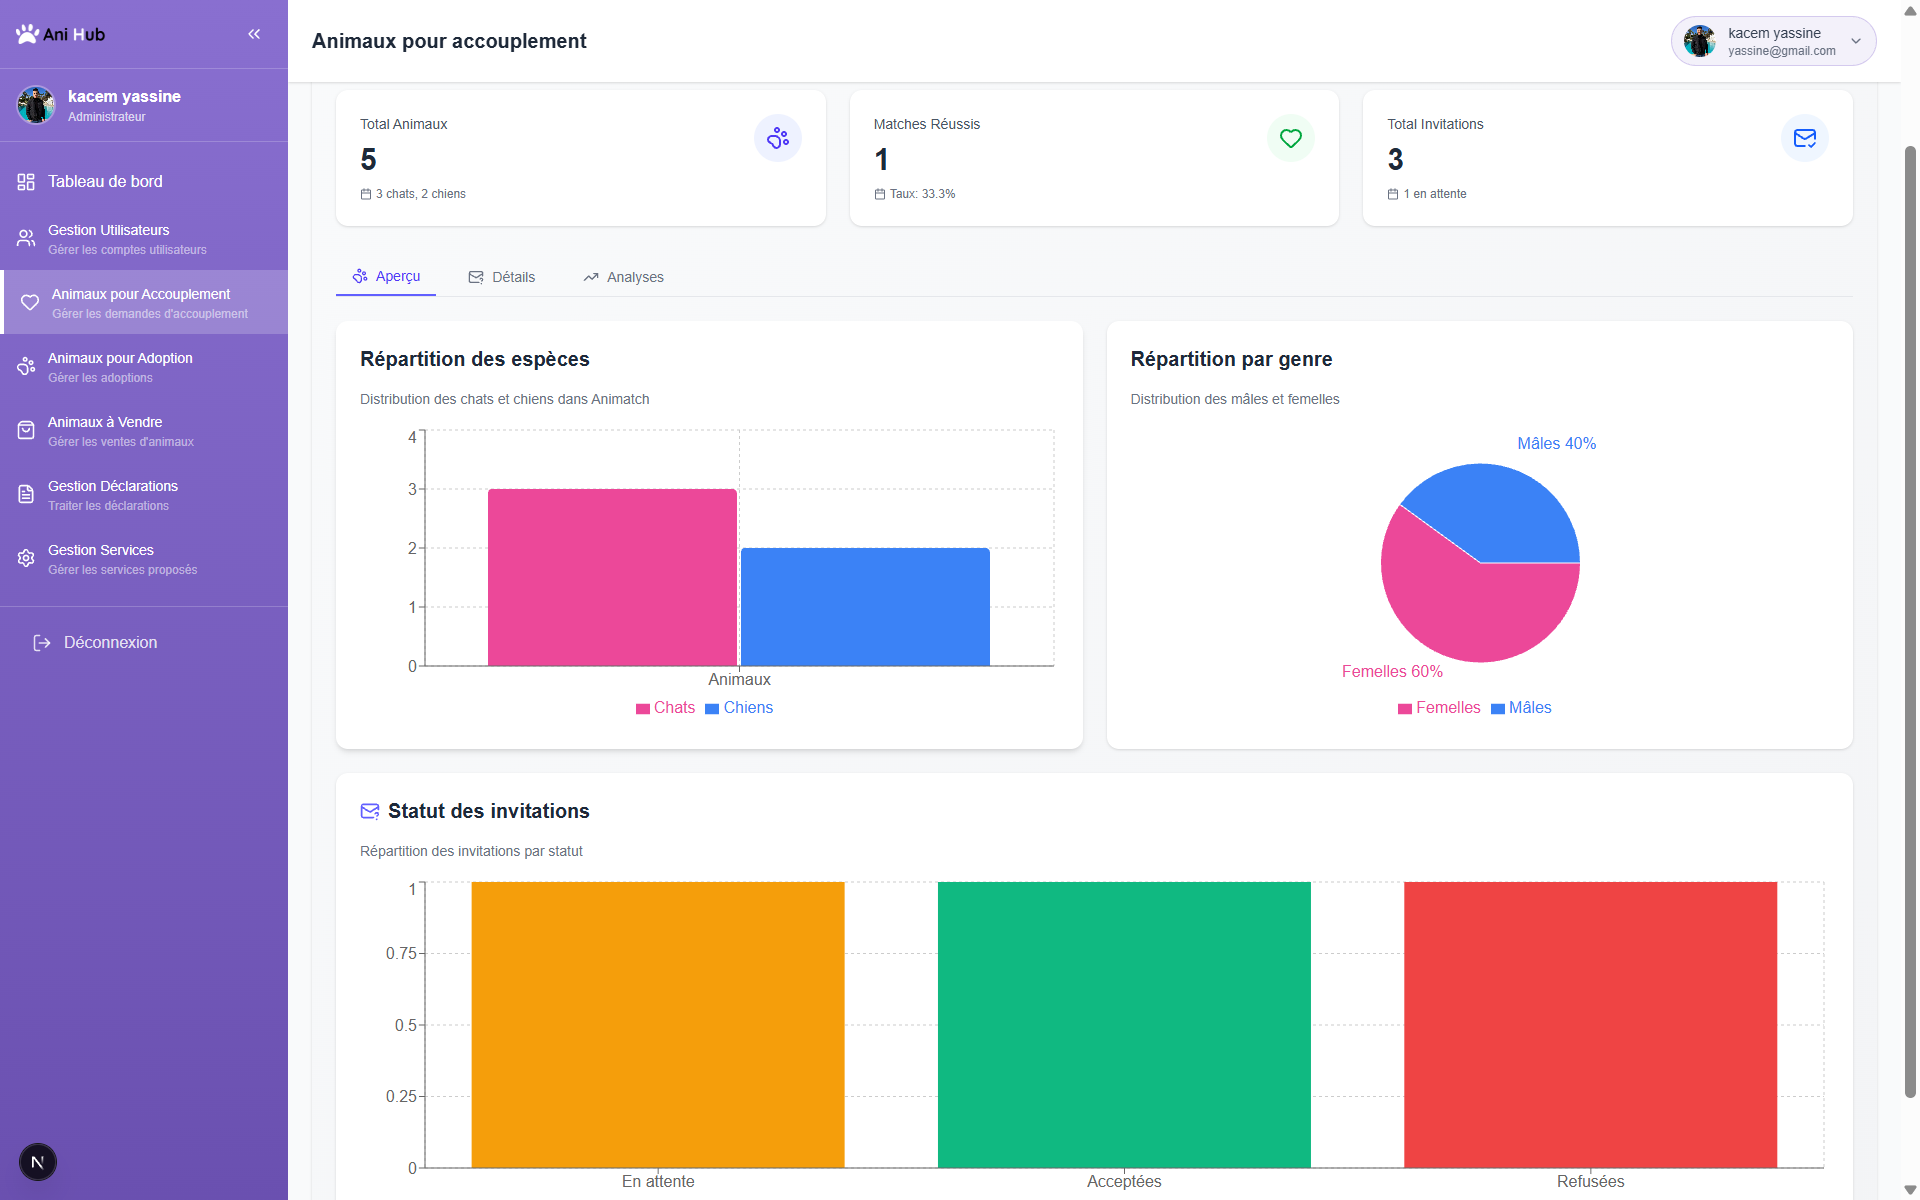
\includegraphics[width=\textwidth]{images/dashboard animatch 2.png}
        \caption{Interface d’administration des statistiques d’AniMatch}
        \label{fig:animatch_stats}
    \end{minipage}

\end{figure}

\subsubsection{Interfaces d’administration pour le module AniFound avec statistiques}  

Les figures \ref{fig:anifound_manage} et \ref{fig:anifound_stats} illustrent les interfaces permettant à l’administrateur de gérer le module AniFound, dédié au signalement des animaux perdus et trouvés, ainsi que de consulter les statistiques associées afin de suivre l’activité et les publications du module : 
\begin{figure}[h!]
    \centering
    
    \begin{minipage}{0.48\textwidth}
        \centering
        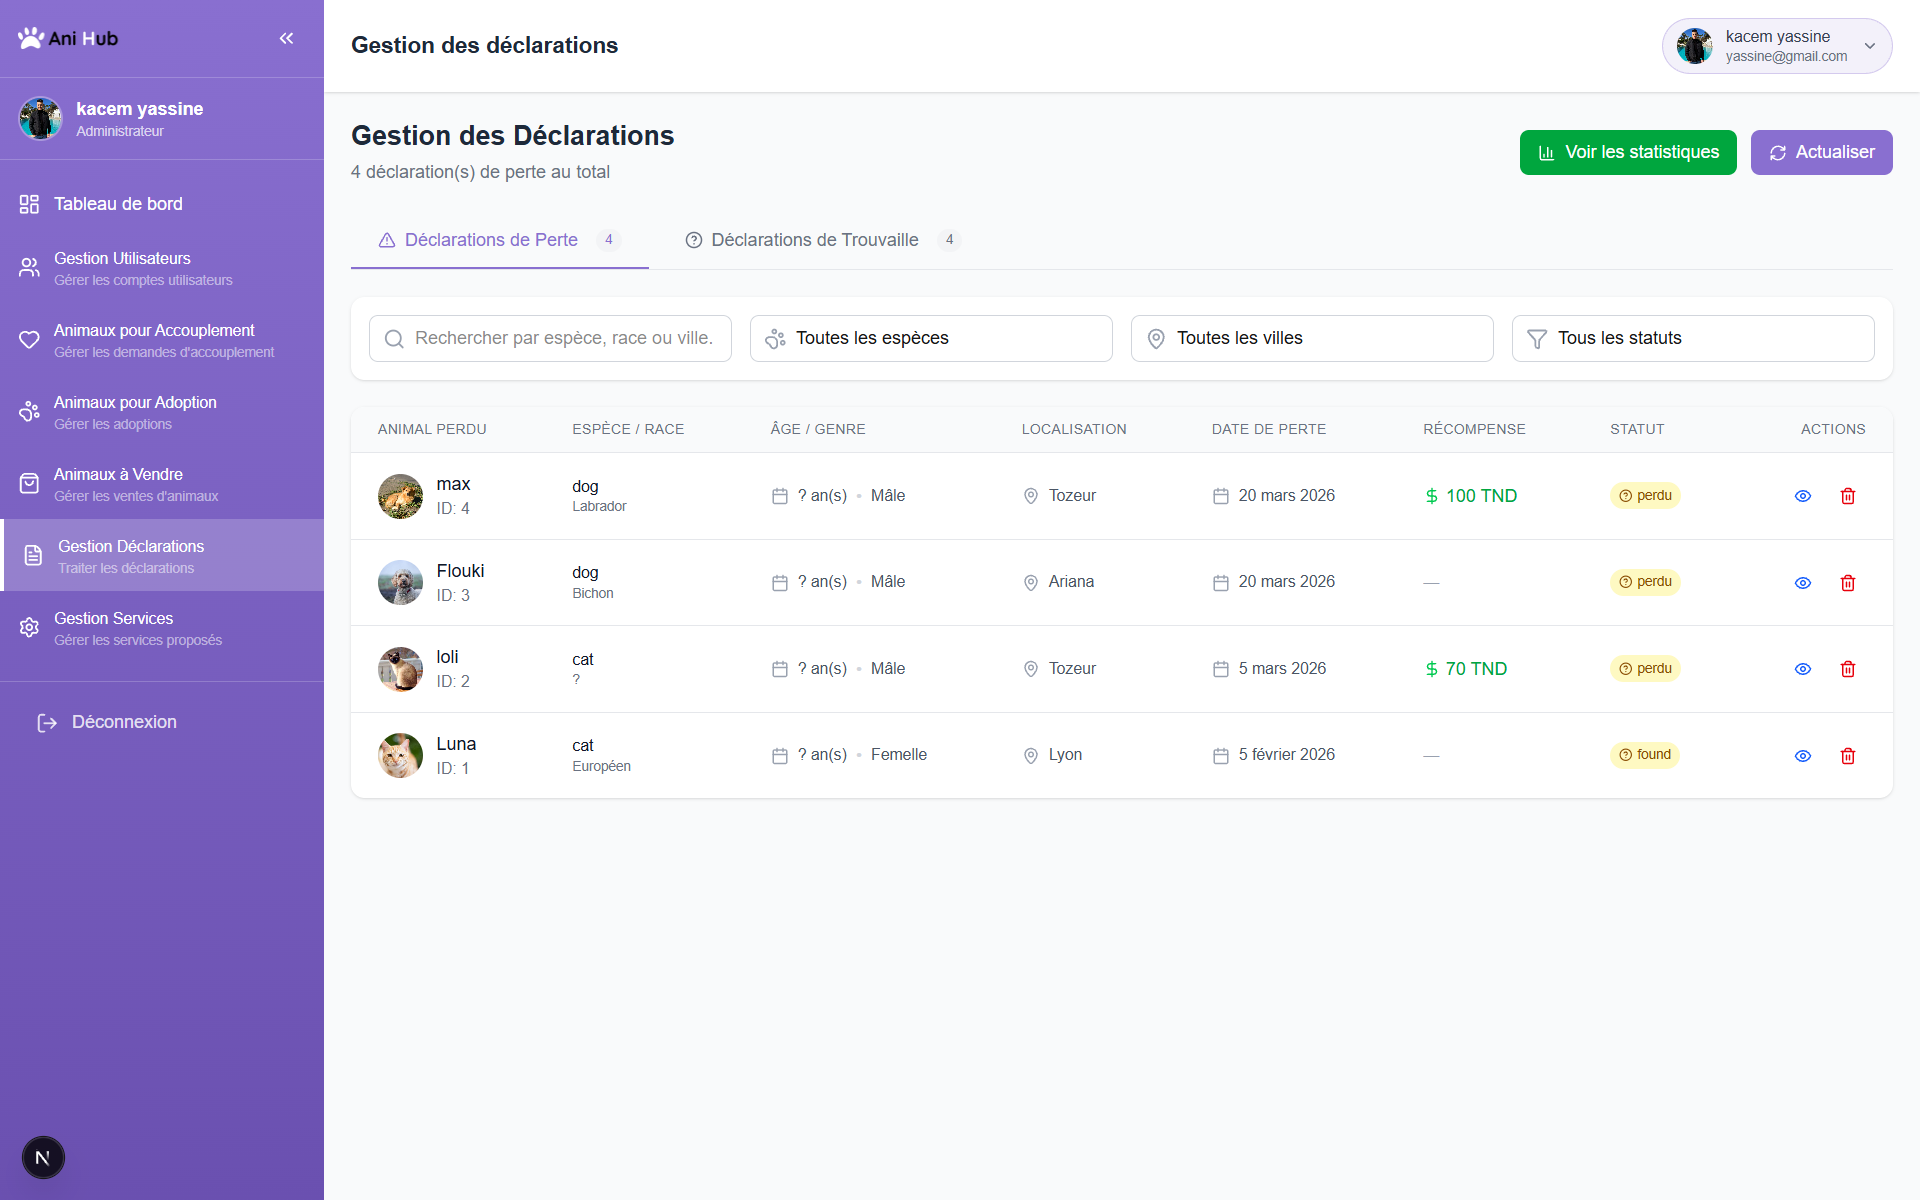
\includegraphics[width=\textwidth]{images/dashboard anifound 1.png}
        \caption{Interface d’administration de gestion d’AniFound}
        \label{fig:anifound_manage}
    \end{minipage}
    \hfill
    \begin{minipage}{0.48\textwidth}
        \centering
        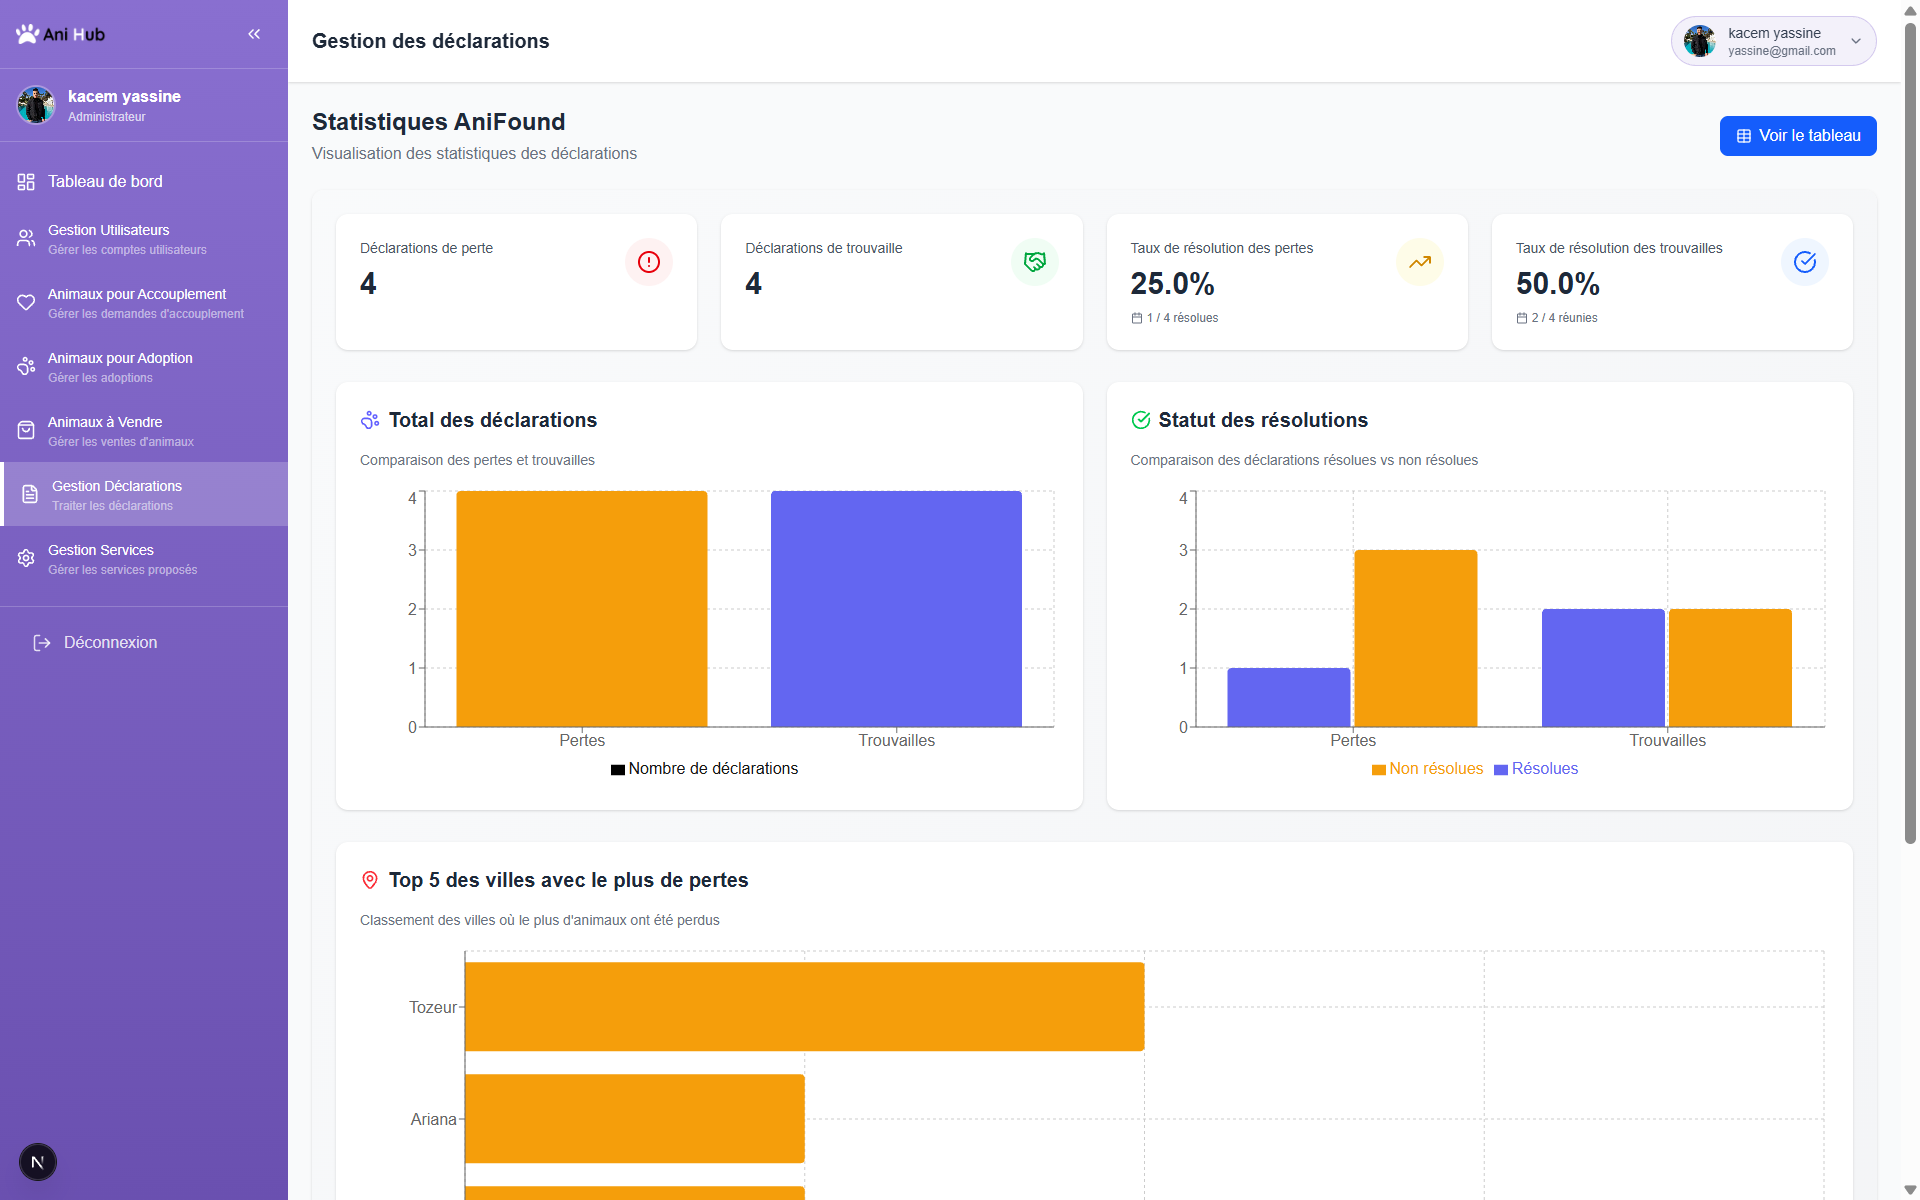
\includegraphics[width=\textwidth]{images/dashboard anifound 2.png}
        \caption{Interface d’administration des statistiques d’AniFound}
        \label{fig:anifound_stats}
    \end{minipage}

\end{figure}

\newpage

\subsubsection{Interfaces d’administration pour le module AniMarket avec statistiques}

Les figures \ref{fig:animarket_manage} et \ref{fig:animarket_stats} illustrent les interfaces permettant à l’administrateur de gérer le module AniMarket (le module de vente, achat et enchères d’animaux en ligne) et de consulter les statistiques associées : 

\begin{figure}[h!]
    \centering

    \begin{minipage}{0.48\textwidth}
        \centering
        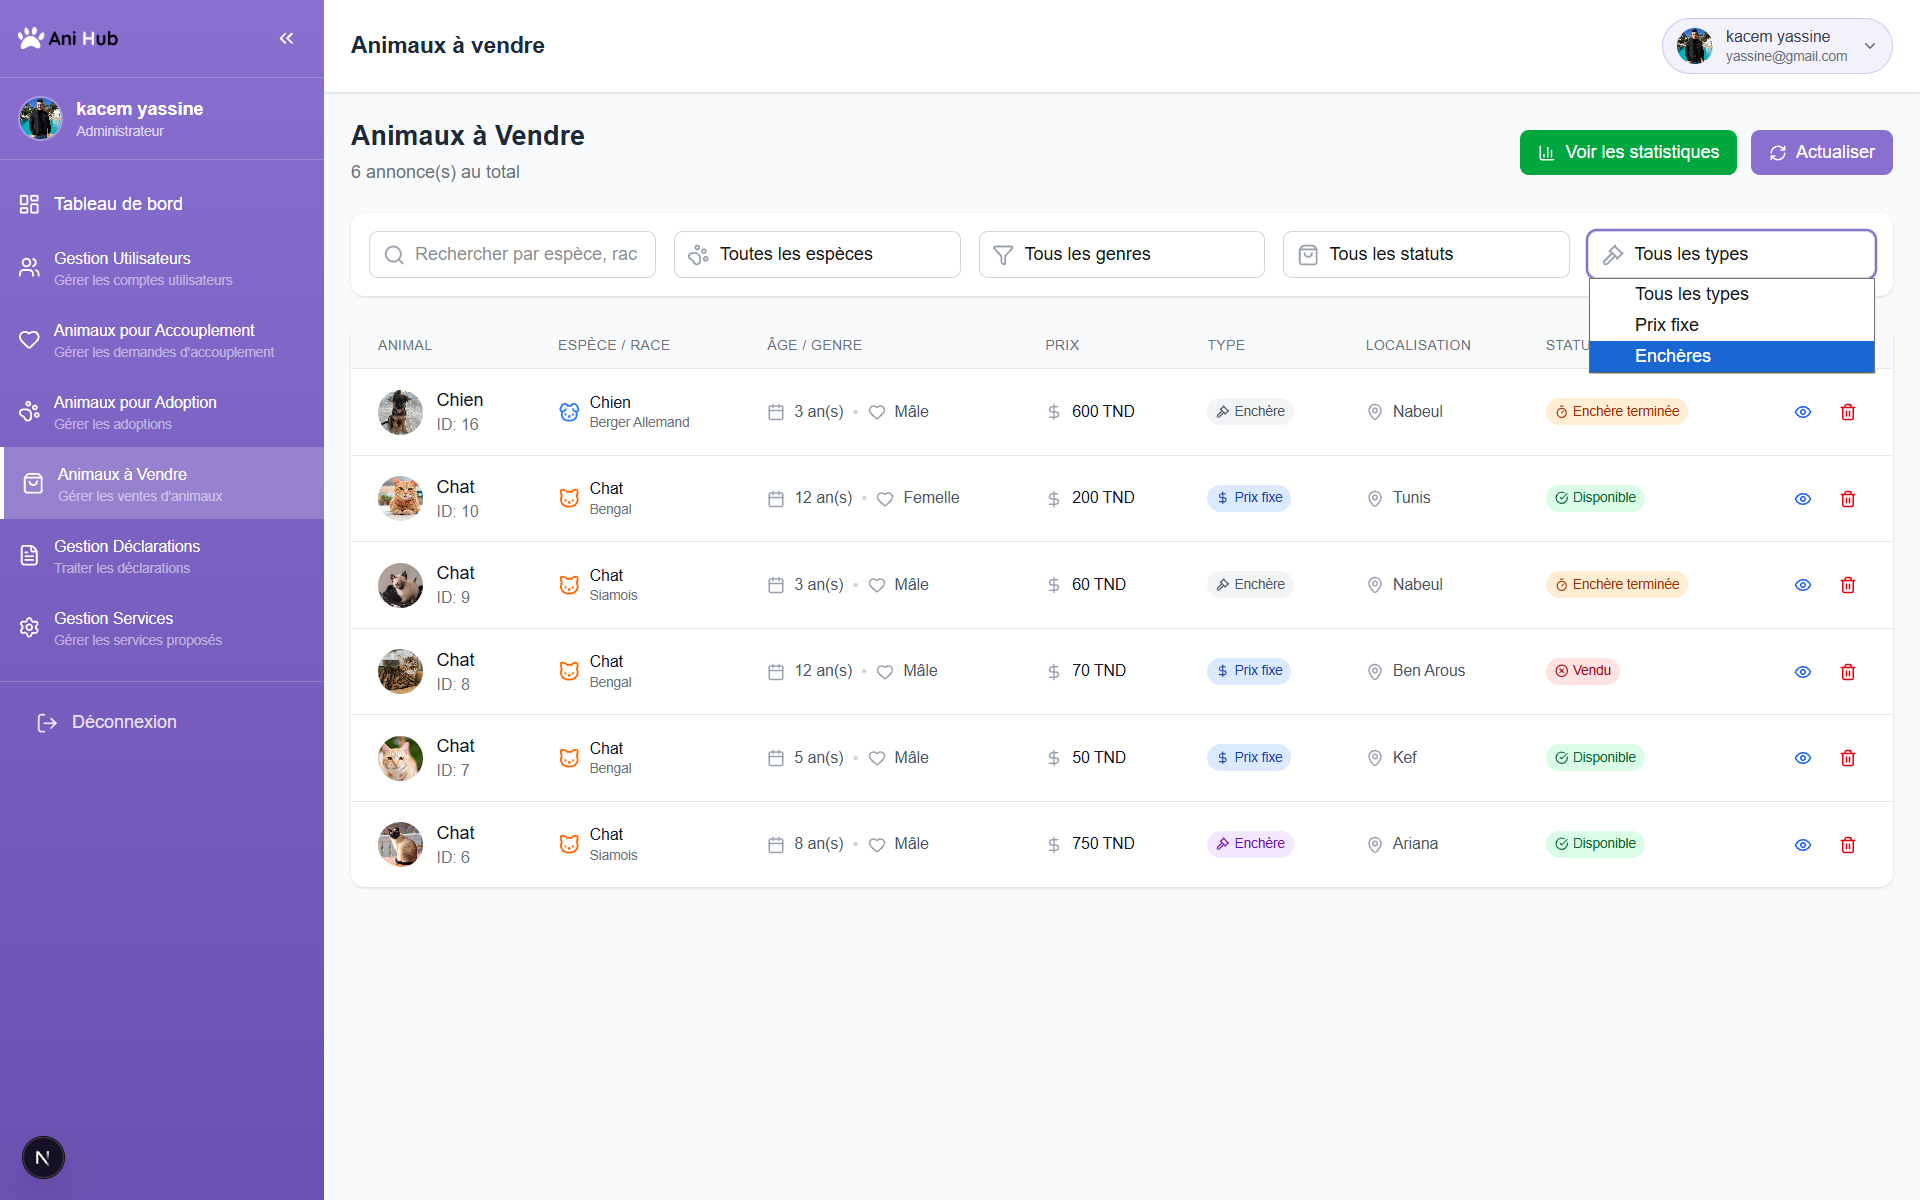
\includegraphics[width=\textwidth]{images/dashboard animarket 1.png}
        \caption{Interface d’administration de gestion d’AniMarket}
        \label{fig:animarket_manage}
    \end{minipage}
    \hfill
    \begin{minipage}{0.48\textwidth}
        \centering
        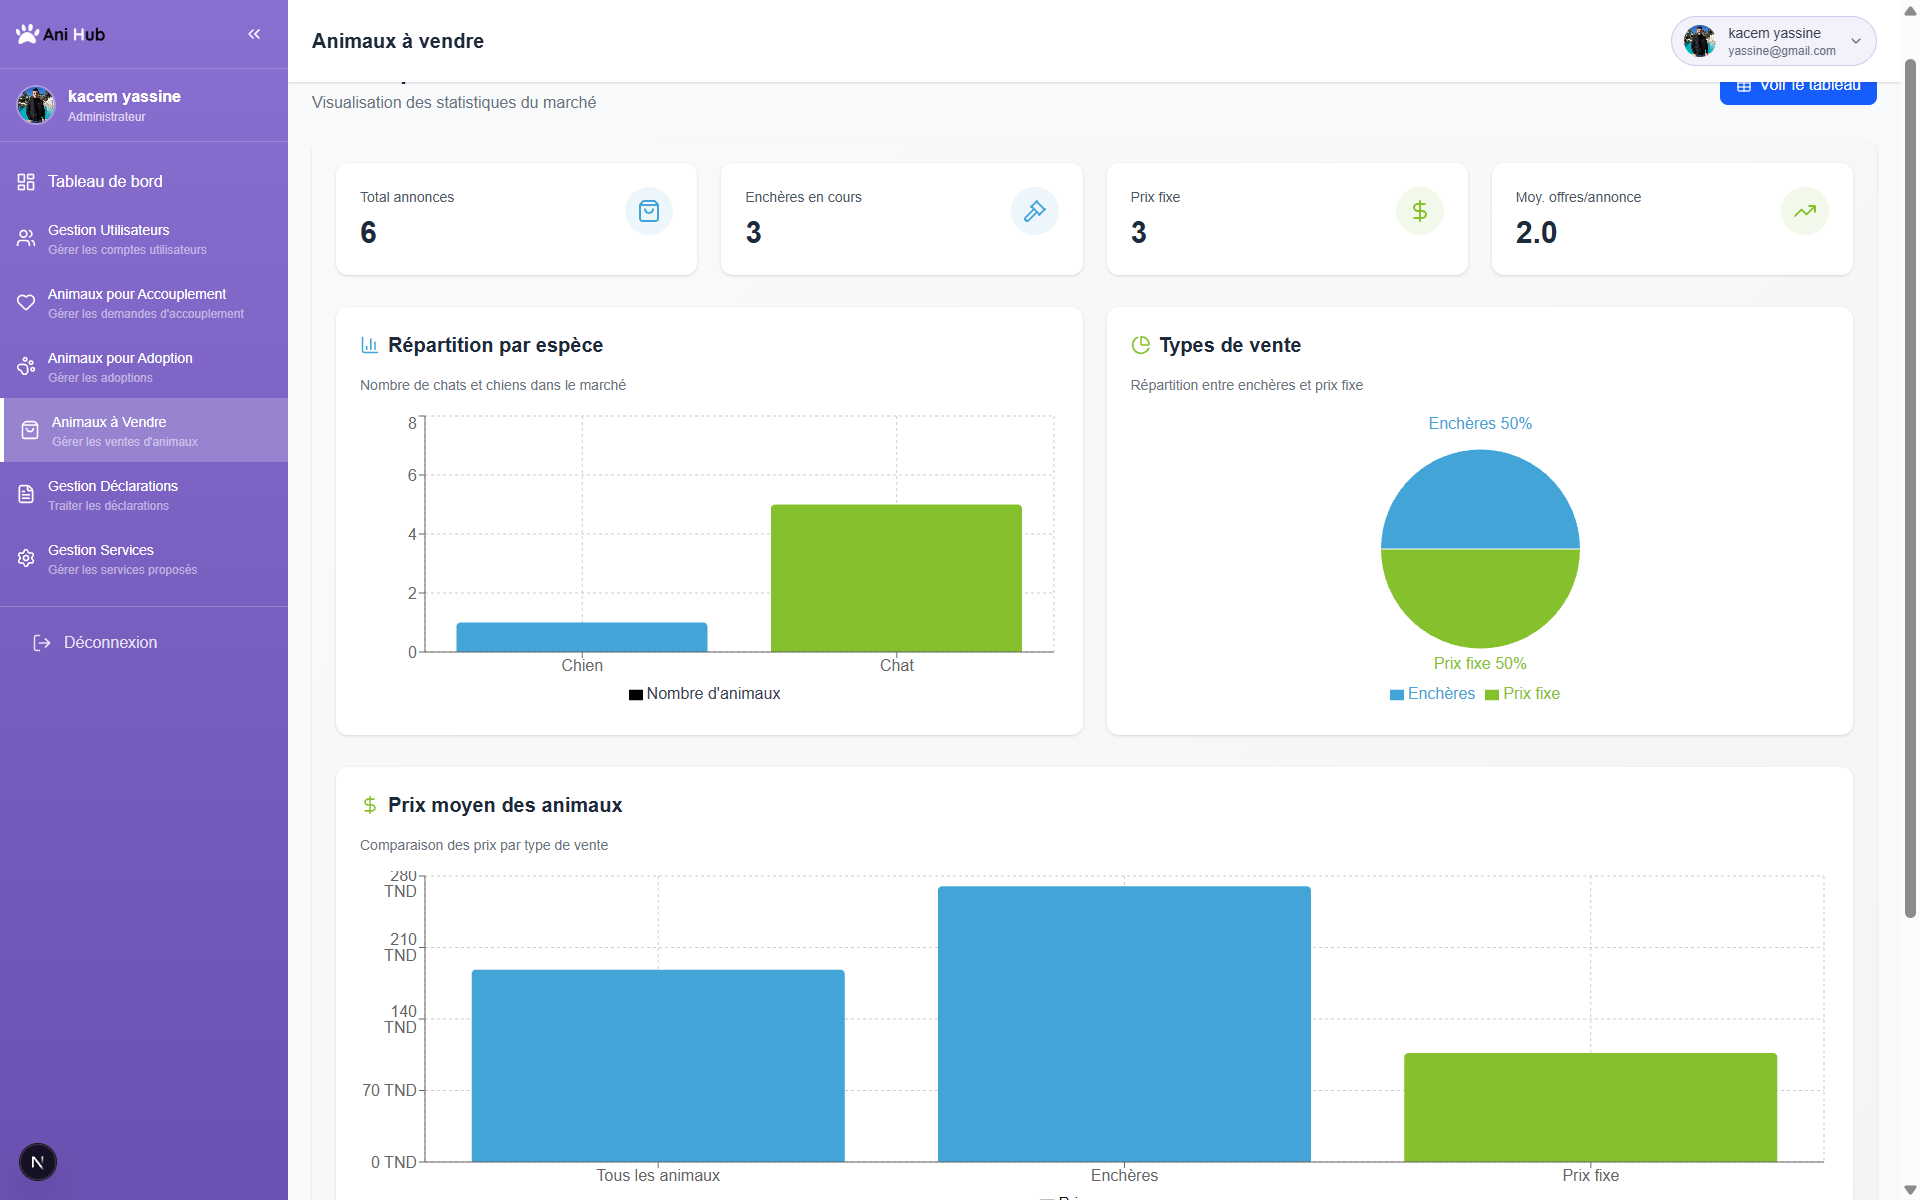
\includegraphics[width=\textwidth]{images/dashboard animarket 2.png}
        \caption{Interface d’administration des statistiques d’AniMarket}
        \label{fig:animarket_stats}
    \end{minipage}

\end{figure}

\subsubsection{Interface d’administration AniCare : gestion des services} 

La figure \ref{fig:anicare_manage} illustre la gestion des services dans le module AniCare, tels que les services de dressage, de soins vétérinaires, de toilettage et de garderie publiés par les prestataires de services : 
\begin{figure}[h!]
    \centering
    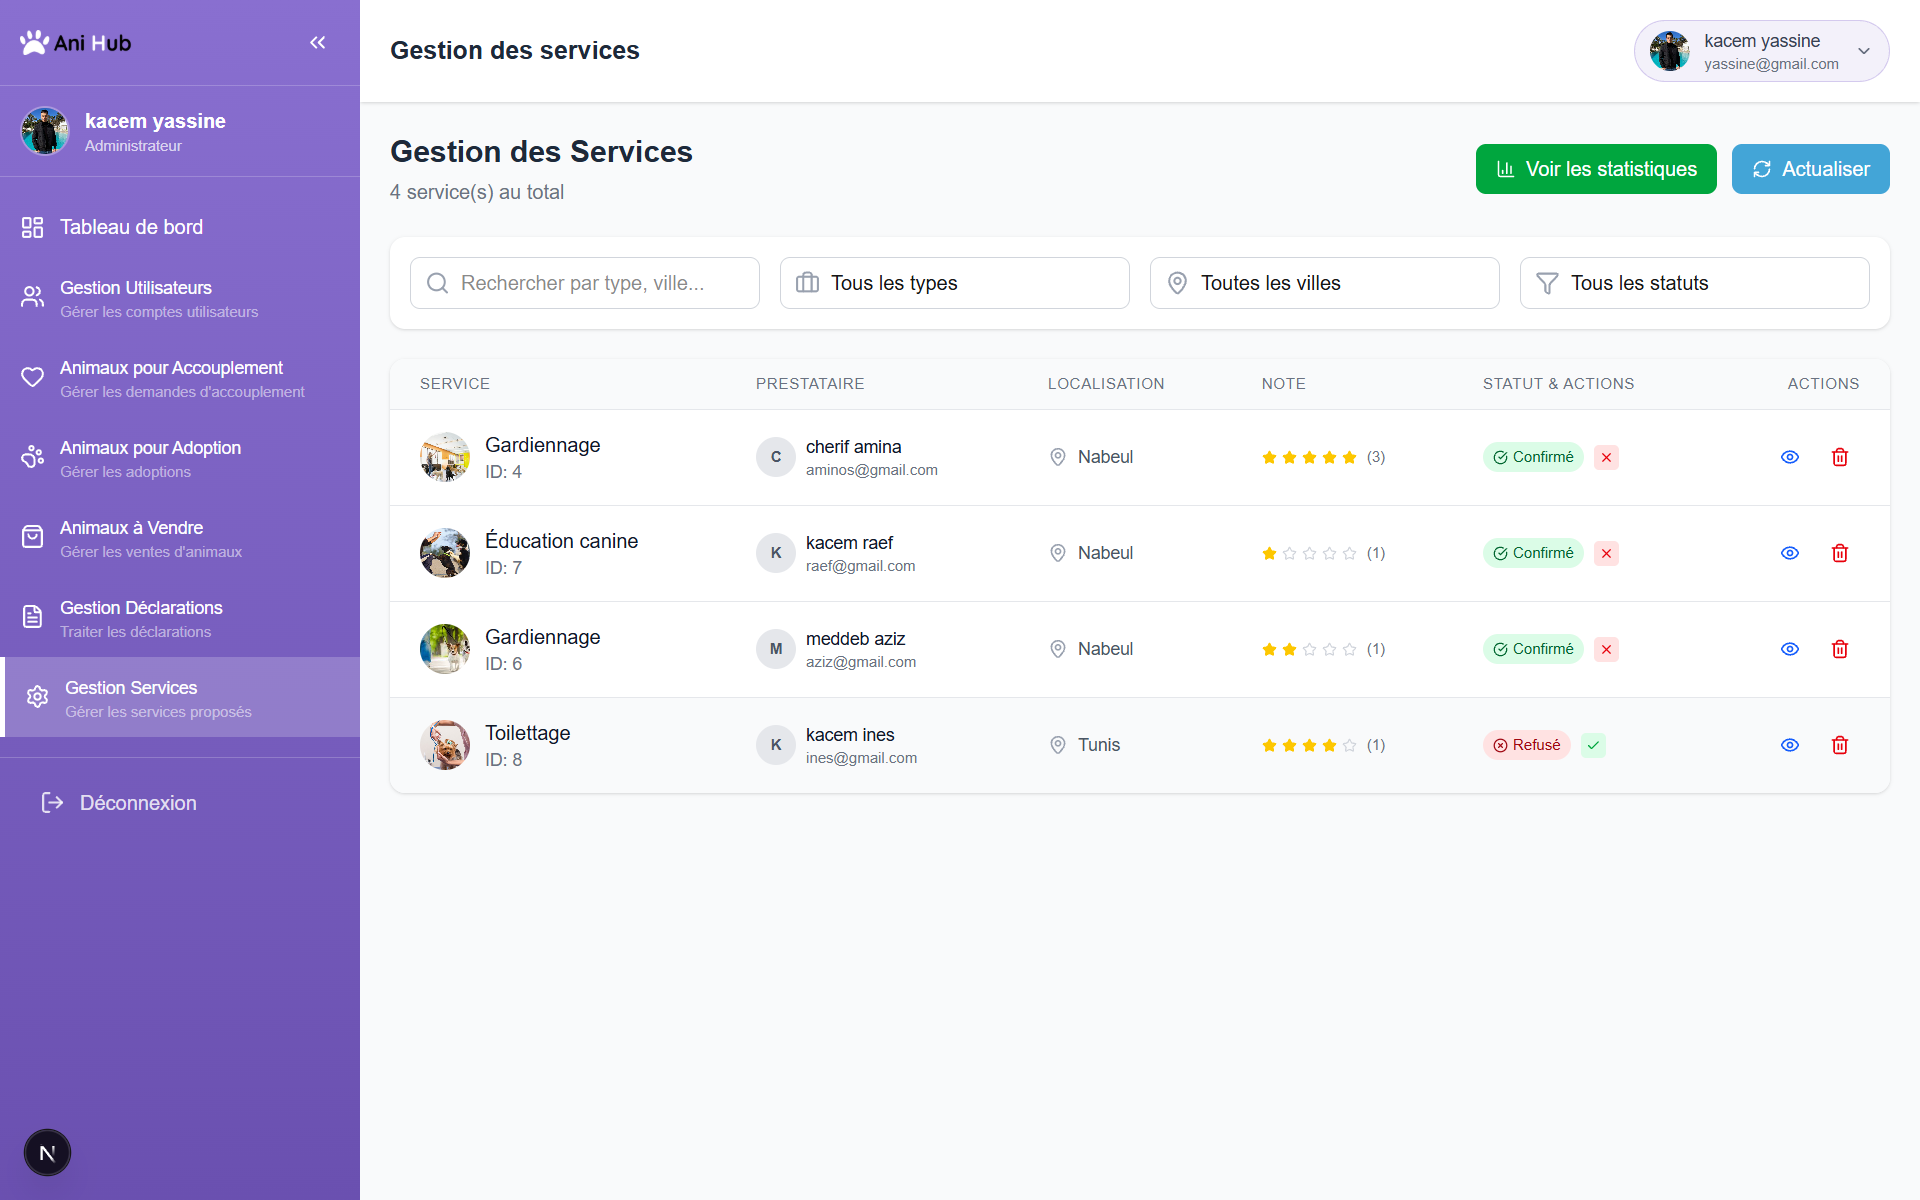
\includegraphics[width=0.8\textwidth]{images/dashboard anicare 1.png}
    \caption{Interface d’administration AniCare : gestion des services}
    \label{fig:anicare_manage}
\end{figure}

\newpage 

\subsubsection{Interface d’administration AniCare : vérification des services} 

La figure \ref{fig:anicare_verify} illustre l’interface de vérification des services dans le module AniCare, qui permet à l’administrateur de vérifier les documents justificatifs fournis par les prestataires de services avant de confirmer leurs services sur la plateforme : 
\begin{figure}[h!]
    \centering
    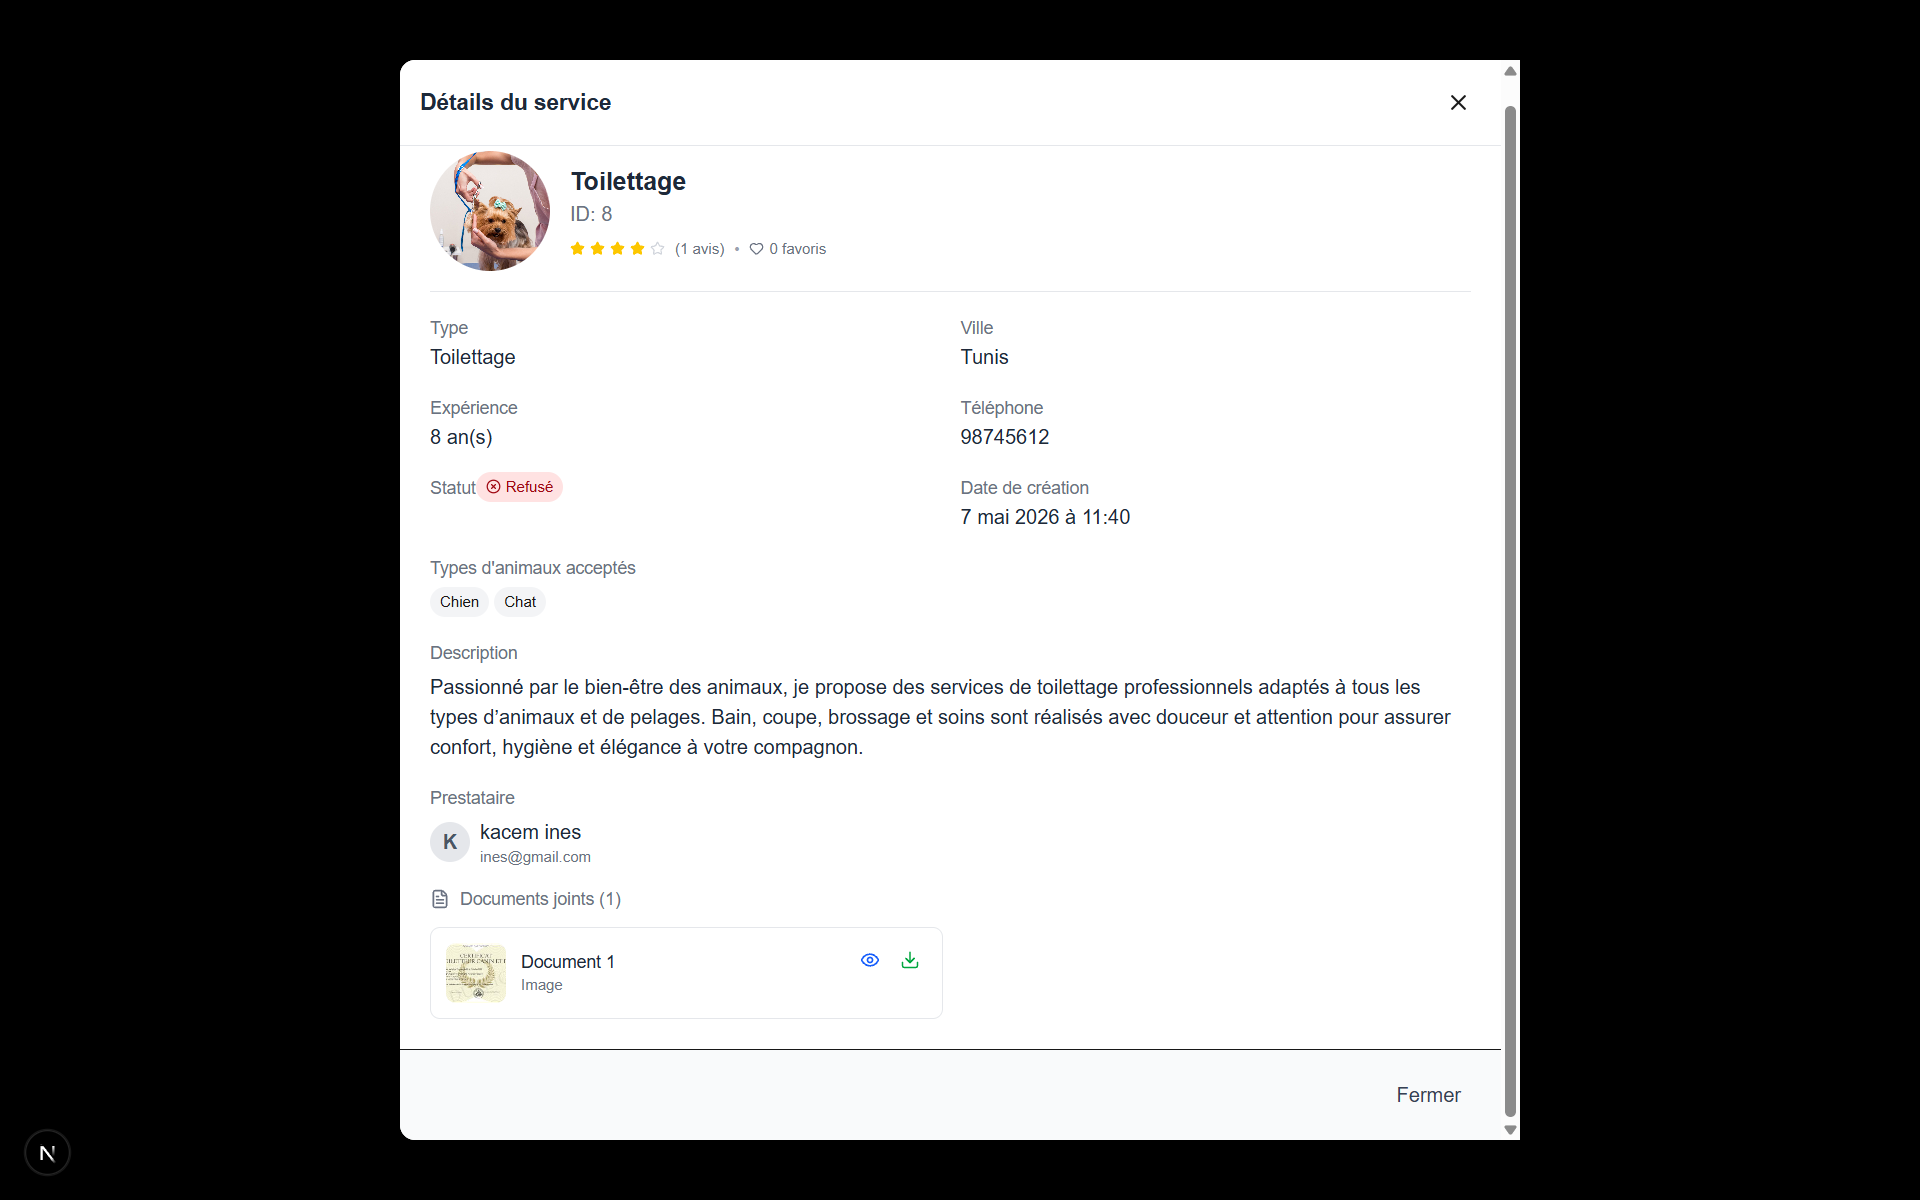
\includegraphics[width=0.8\textwidth]{images/dashboard anicare 2.png}
    \caption{Interface d’administration AniCare : vérification des services}
    \label{fig:anicare_verify}
\end{figure}

\subsubsection{Interfaces d’administration AniCare : statistiques AniCare}

Les figures \ref{fig:anicare_stats1} et \ref{fig:anicare_stats2} illustrent les statistiques du module AniCare, permettant à l’administrateur de suivre l’activité des services proposés sur la plateforme, le nombre de réservations effectuées ainsi que les interactions des utilisateurs avec les différents services disponibles : 
\begin{figure}[h!]
    \centering

    \begin{minipage}{0.48\textwidth}
        \centering
        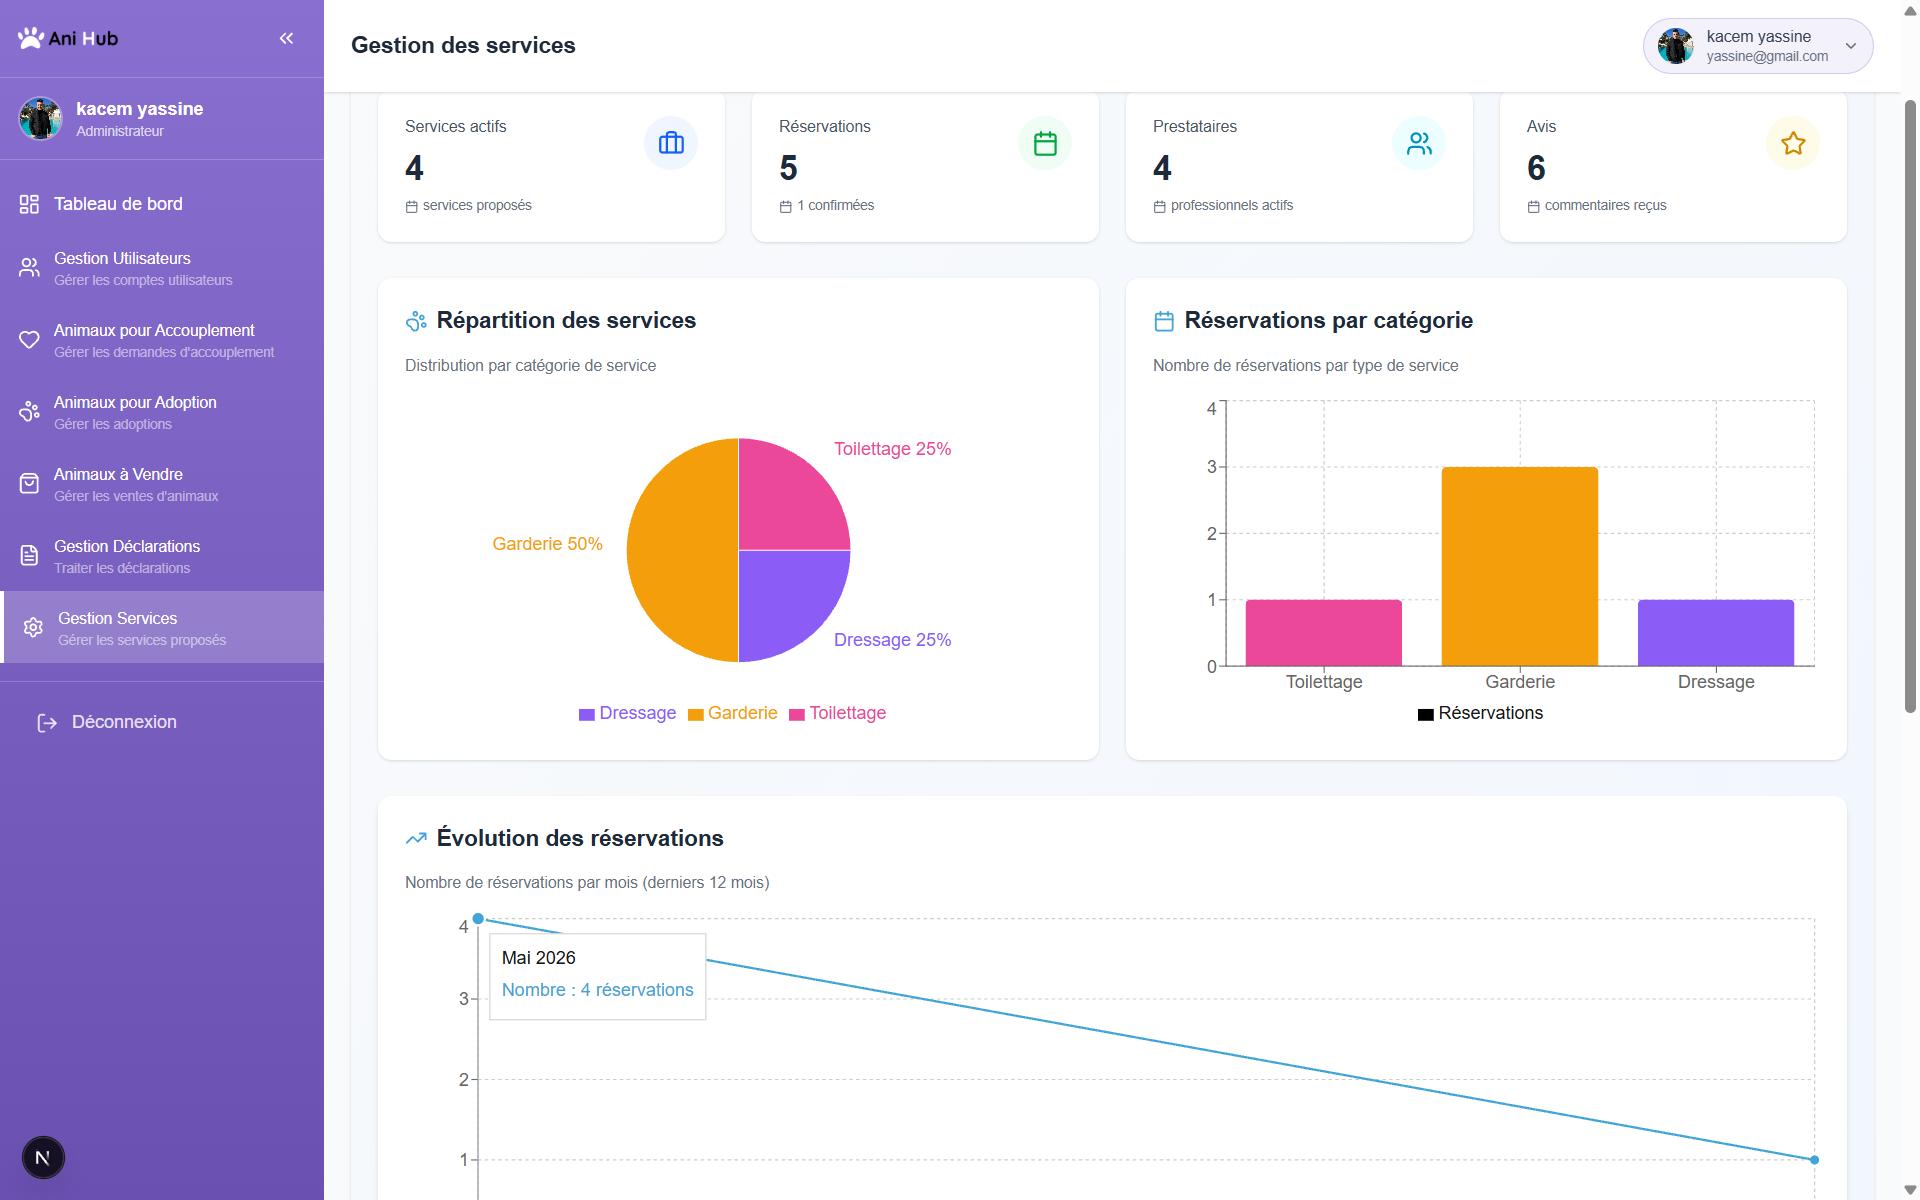
\includegraphics[width=\textwidth]{images/dashboard anicare 3.png}
        \caption{Interface de statistiques AniCare 1}
        \label{fig:anicare_stats1}
    \end{minipage}
    \hfill
    \begin{minipage}{0.48\textwidth}
        \centering
        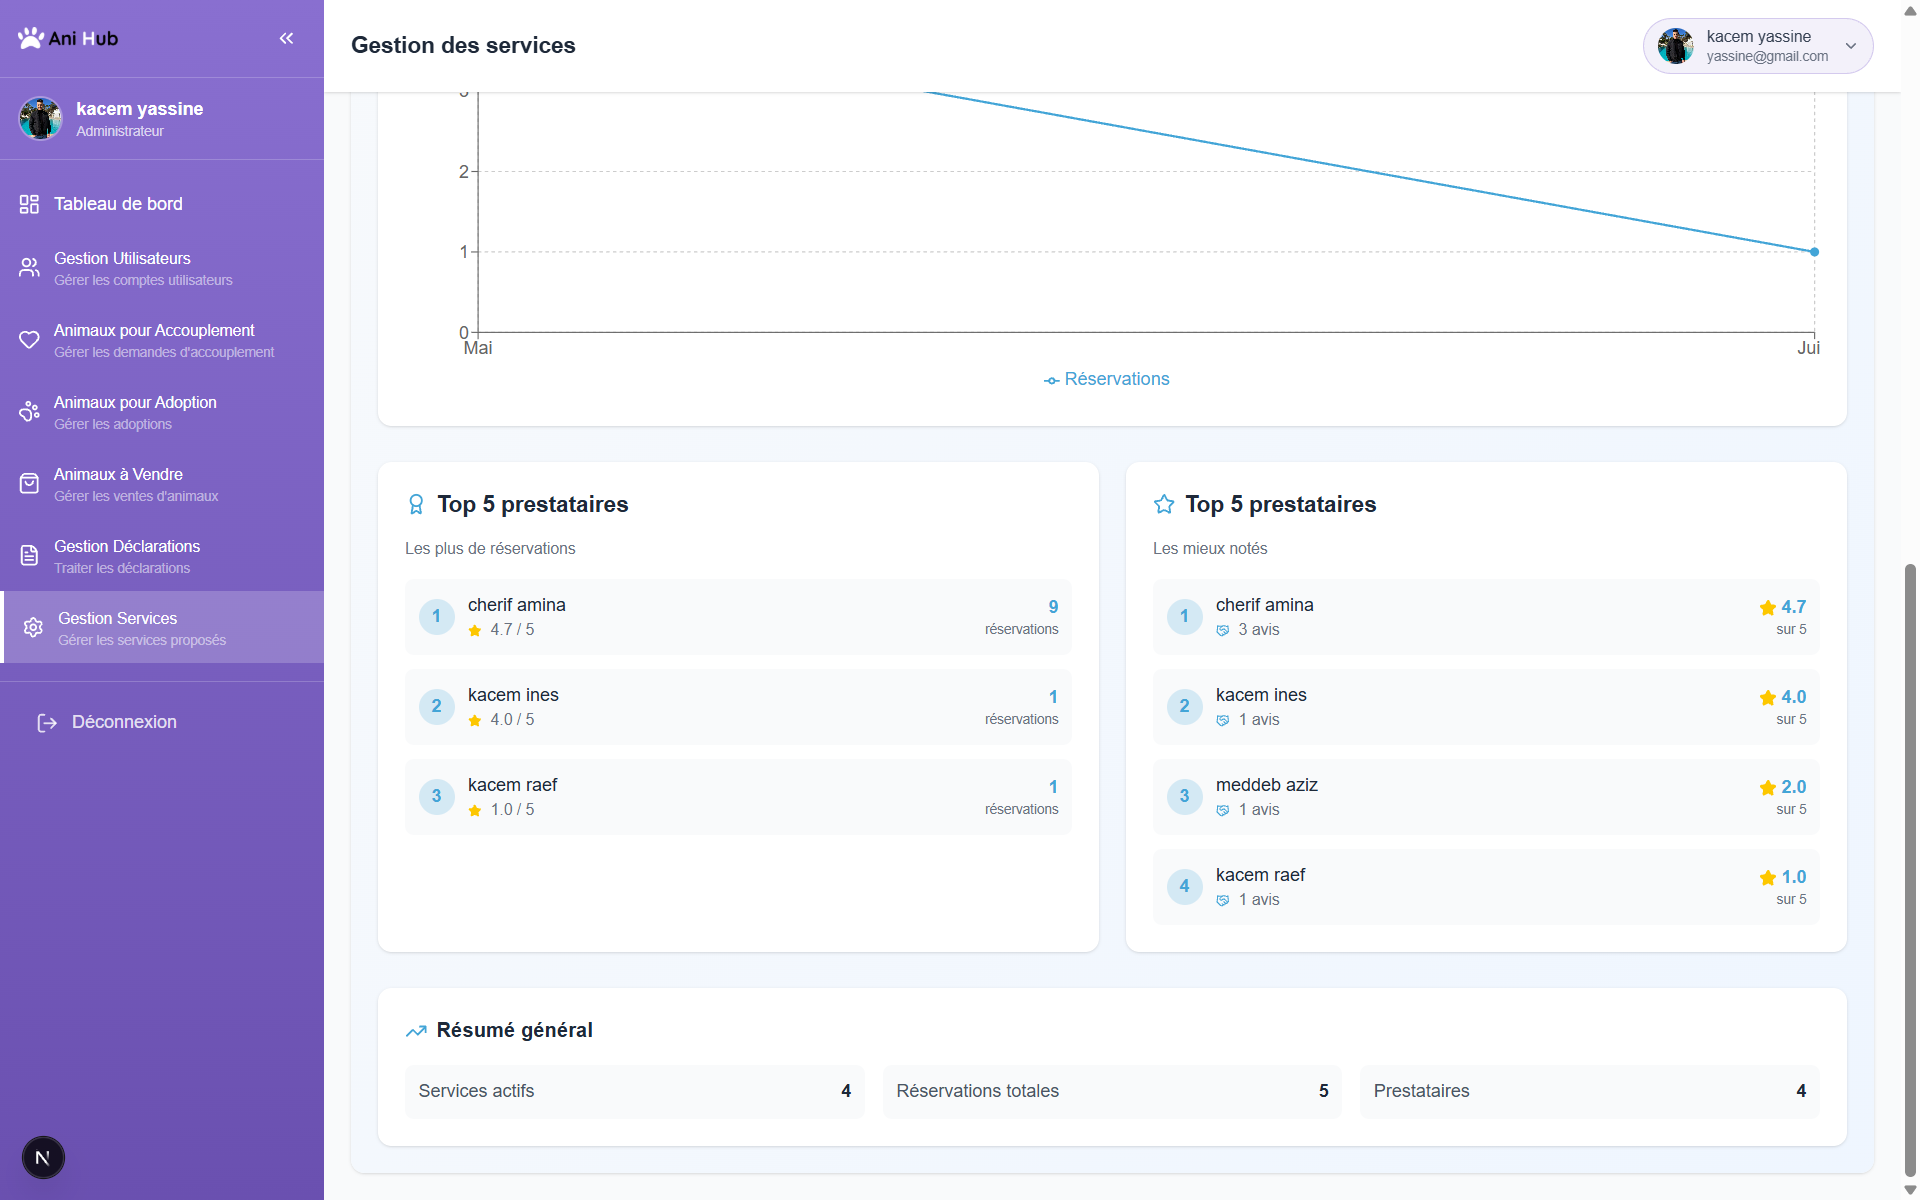
\includegraphics[width=\textwidth]{images/dashboard anicare 4.png}
        \caption{Interface de statistiques AniCare 2}
        \label{fig:anicare_stats2}
    \end{minipage}
\end{figure}






\section{Sprint 2 : Module AniMatch}
\begin{figure}[H]
    \centering
    
\includegraphics[width=3.8cm]{images/logo animatch 2.png}
    \caption{Logo du module AniMatch}
    \label{fig:logo-animatch}
\end{figure}
Ce sprint, d’une durée de \textbf{3 semaines}, est dédié au module AniMatch, qui permet la mise en relation entre propriétaires d’animaux pour l’adoption et l’accouplement. Il offre la possibilité de publier et consulter des annonces, d’échanger des invitations et de communiquer entre utilisateurs.  



\subsection{Sprint backlog} 
la table \ref{tab:sprint2-backlog} présente le Sprint Backlog du sprint 2 avec les user stories, les tâches associées et les efforts estimés : 
\begin{longtable}{|p{2cm}|p{5cm}|p{6cm}|p{2cm}|}
\caption{Sprint Backlog du sprint 2 }
\label{tab:sprint2-backlog} \\ 
\hline
\rowcolor{coloranimatch}
\textbf{ID} & \textbf{User Story} & \textbf{Tâches} & \textbf{Effort} \\
\hline
\endfirsthead

\hline
\rowcolor{coloranimatch}
\textbf{ID} & \textbf{User Story} & \textbf{Tâches} & \textbf{Effort} \\
\hline
\endhead

% ===================== US1=====================
\multirow{9}{2cm}{US1}
& \multirow{9}{5cm}{En tant qu’utilisateur, je
veux consulter la liste des animaux (adoption ou accouplement) afin de trouver un partenaire compatible}
& Conception UI (Figma) & 0.5 j \\
\cline{3-4}
& & API récupération des animaux & 1 j \\
\cline{3-4}
& & Filtrage et recherche & 1 j \\
\cline{3-4}
& & Pagination & 0.5 j \\
\cline{3-4}
& & Commentaires et notation des animaux & 1 j \\
\cline{3-4}
& & Intégration frontend/backend & 1 j \\
\hline

% ===================== US2 =====================
\multirow{10}{2cm}{US2}
& \multirow{10}{5cm}{En tant qu’utilisateur, je veux gérer mes annonces (publier, modifier et supprimer mes animaux) afin de maintenir mes informations à jour et trouver une correspondance}
& Conception UI (Figma) & 0.5 j \\
\cline{3-4}
& & APIs création , modification et suppression annonce & 1 j \\
\cline{3-4} 
& & Intégration avec microservice Auth (JWT, sécurité API) & 0.5 j \\
\cline{3-4}
& & Upload image (Cloudinary) & 1 j \\
\cline{3-4}
& & Intégration frontend/backend & 1 j \\ 
\cline{3-4} 
& & Tests & 0.5 j \\
\hline

% ===================== US3 =====================
\multirow{8}{2cm}{US3}
& \multirow{8}{5cm}{En tant qu’utilisateur, je veux gérer mes invitations envoyées afin de contrôler mes interactions}
& Conception UI "mon espace AniMatch"  (Figma) & 0.5 j \\
\cline{3-4}
& & API envoi, modification et annulation invitation & 1 j \\
\cline{3-4}
& & Gestion des statuts (en attente, acceptée, refusée) & 1 j \\ 
\cline{3-4} 
& & Intégration avec microservice Auth (JWT, sécurité API) & 0.5 j \\
\cline{3-4}
& & Intégration frontend/backend & 1 j \\
\hline

% ===================== US4 =====================
\multirow{5}{2cm}{US4}
& \multirow{5}{5cm}{En tant qu’utilisateur, je veux gérer les invitations reçues pour adoption ou accouplement afin de répondre aux demandes et gérer mes interactions}
& Conception UI (Figma) & 0.5 j \\
\cline{3-4}
& & API récupération des invitations reçues & 1 j \\
\cline{3-4}
& & APIs accepter , refuser invitation & 1 j \\
\cline{3-4}
& &  Gestion des statuts (acceptée, refusée)  & 0.5 j \\
\cline{3-4}
& & Intégration avec microservice Auth (JWT, sécurité API) & 0.5 j \\ 
\cline{3-4} 
& & Intégration frontend/backend & 1 j \\ 
\cline{3-4}  
\cline{3-4}
& & Tests & 0.5 j \\
\hline

% ===================== US5 =====================
\multirow{6}{2cm}{US5}
& \multirow{6}{5cm}{En tant qu’utilisateur, je veux gérer mes notifications afin d’être informé des interactions sur mes annonces et activités sur Animatch}
& Analyse besoins notifications & 0.5 j \\
\cline{3-4}
& & Développement microservice Notifications & 1 j \\
\cline{3-4}
& & Intégration RabbitMQ avec Microservice AniMatch & 1 j \\
\cline{3-4}
& & Intégration RabbitMQ avec Microservice Notifications & 1 j \\
\cline{3-4}
& & Création événements (invitations, intérêts, acceptation, etc.) & 0.5 j \\
\cline{3-4}
& & Interface notifications frontend & 0.5 j \\
\cline{3-4}
& & Marquer comme lu / non lu & 0.5 j \\ 
\cline{3-4}
& & Tests & 0.5 j \\
\hline

% ===================== US8 =====================
\multirow{4}{2cm}{US6}
& \multirow{4}{5cm}{En tant qu’utilisateur, je veux discuter avec un autre propriétaire}
& Analyse & 0.5 j \\
\cline{3-4}
& & Intégration bouton WhatsApp & 0.5 j \\
\cline{3-4}
& & Génération lien wa.me & 0.5 j \\
\cline{3-4}
& & Tests & 0.5 j \\
\hline

\end{longtable}
\newpage
\subsection{Diagramme des cas d’utilisation du sprint 2}

Dans cette section, nous présentons le diagramme des cas d’utilisation du deuxième sprint, dédié au module \textbf{AniMatch}. 

 Ce diagramme illustre les principales interactions entre l’utilisateur et le système, notamment la gestion des annonces, des invitations et des communications.

La figure \ref{fig:usecase-sprint2} représente le diagramme des cas d’utilisation correspondant.

\begin{figure}[H]
    \centering
  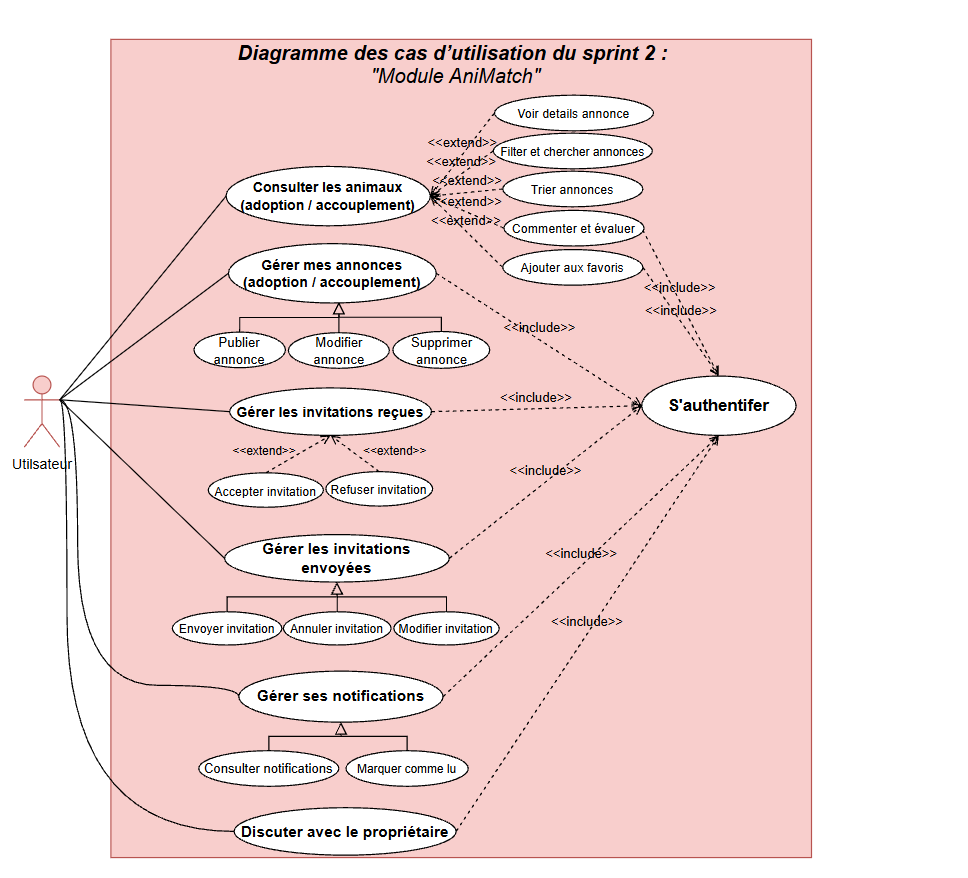
\includegraphics[width=1.05\linewidth, height=19.5cm, keepaspectratio]{images/usecase animatch.png}
    \caption{Diagramme des cas d’utilisation du sprint 2}
    \label{fig:usecase-sprint2}
\end{figure}


\newpage
\subsection{Descriptions textuelles des cas d’utilisation du sprint 2}   
Cette section présente les cas d’utilisation du sprint 2 du module AniMatch : 
\subsubsection{ Description textuelle du cas d’utilisation «Consulter les animaux pour adoption et accouplement» } 
La table \ref{tab:consulter_annonces} présente le cas d’utilisation « Consulter les animaux pour adoption et accouplement » : 
\begin{longtable}{|c|p{11cm}|}
\caption{Description textuelle du cas d’utilisation "Consulter les animaux pour adoption et accouplement"}
\label{tab:consulter_annonces} \\
\hline
\cellcolor{coloranimatch} \textbf{Nom du cas d'utilisation } & Consulter les annonces d’accouplement et d’adoption \\
\hline
\cellcolor{coloranimatch} \textbf{Acteurs} & Utilisateur \\
\hline
\cellcolor{coloranimatch} \textbf{Description } & Tout utilisateur du site peut consulter les annonces du module AniMatch, notamment celles d’adoption et d’accouplement. \\
\hline
\cellcolor{coloranimatch} \textbf{Pré-condition } & Accès libre à la page d’accueil sans authentification. \\
\hline
\cellcolor{coloranimatch} \textbf{Post-condition } & L’utilisateur a consulté les annonces et peut interagir . \\
\hline

\cellcolor{coloranimatch} \textbf{Scénario nominal } & 
\begin{enumerate}
\item L’utilisateur accède à la page d’accueil d’AniHub.
\item L’utilisateur choisit le module AniMatch.
\item Le système redirige l’utilisateur vers AniMatch.
\item L’utilisateur choisit "adoption" ou "accouplement".
\item Le système redirige vers la section choisie.
\item L’utilisateur peut filtrer les annonces selon des critères.
\item Le système affiche la liste des annonces filtrés.
\item L’utilisateur clique sur une annonce .
\item Le système affiche les détails de l’annonce.
\item L’utilisateur authentifié ajoute une annonce à sa (wishlist).
\item Le système ajoute l’annonce à sa wishlist .
\item L’utilisateur authentifié peut saisir un commentaire , attribuer une note clique sur « Publier ».
\item Le système vérifie , enregistre le commentaire et la note et met à jour la liste des avis affichés.
\end{enumerate} \\

\hline
\cellcolor{coloranimatch} \textbf{Scénario alternatif :} &
Message d’erreur affiché si l’utilisateur n’est pas authentifié lors de l’ajout aux favoris ou de la publication d’un commentaire. \\
\hline

\end{longtable}


\newpage 
\subsubsection{Description textuelle du cas d’utilisation «Gérer mes annonces dans AniMatch»} 
La table \ref{tab:gerer_annonces_global} présente le cas d’utilisation « Gérer mes  annonces d’accouplement et d’adoption » : 
\begin{longtable}{|c|p{11cm}|}
\caption{Description textuelle du cas d'utilisation "Gérer les annonces d’accouplement et d’adoption"}
\label{tab:gerer_annonces_global} \\
\hline
\cellcolor{coloranimatch}\textbf{Nom du cas d'utilisation } & Gérer mes annonces d’accouplement et d’adoption \\
\hline
\cellcolor{coloranimatch}\textbf{Acteurs} & Utilisateur \\
\hline
\cellcolor{coloranimatch}\textbf{Description } & L’utilisateur peut publier, modifier ou supprimer une annonce \\
\hline
\cellcolor{coloranimatch}\textbf{Pré-condition } & L’utilisateur doit être authentifié  \\
\hline
\cellcolor{coloranimatch}\textbf{Post-condition } & L’annonce est ajoutée, modifiée ou supprimée avec succès. \\
\hline

\cellcolor{coloranimatch}\textbf{Scénario nominal } &
\begin{enumerate}
\item L’utilisateur accède au module AniMatch.
\item Le système redirige l’utilisateur vers "AniMatch".

\item \textbf{Cas publication :}
\begin{itemize}
\item L’utilisateur choisit "adoption" ou "accouplement".
\item Le système redirige vers la section choisie.
\item L’utilisateur clique sur « Annoncer mon animal ».
\item Le système affiche le formulaire d’ajout.
\item L’utilisateur remplit les informations et valide.
\item Le système vérifie et enregistre l’annonce.
\end{itemize}

\item L’utilisateur accède à « Mon espace AniMatch ».
\item Le système affiche ses annonces.

\item \textbf{Cas modification :}
\begin{itemize}
\item L’utilisateur sélectionne une annonce.
\item L’utilisateur clique sur « Modifier ».
\item Le système affiche le formulaire pré-rempli.
\item L’utilisateur modifie et valide.
\item Le système enregistre les modifications.
\end{itemize}

\item \textbf{Cas suppression :}
\begin{itemize}
\item L’utilisateur sélectionne une annonce.
\item L’utilisateur clique sur « Supprimer ».
\item Le système demande une confirmation.
\item L’utilisateur confirme.
\item Le système supprime l’annonce.
\end{itemize}

\item Le système affiche un message de succès.
\end{enumerate} \\

\hline
\cellcolor{coloranimatch}\textbf{Scénario alternatif :} &
\begin{itemize}
\item Erreur de publication ou modification : message d’erreur affiché.
\item Annulation de la suppression : l’annonce est conservée.
\end{itemize} \\
\hline

\end{longtable}
\newpage
\subsubsection{ Description textuelle du cas d’utilisation «Gérer les invitations reçues» }   
La table \ref{tab:gerer_invitations} illustre la description textuelle du cas d’utilisation « Gérer les invitations reçues d’accouplement et d’adoption », qui détaille les différentes interactions entre l’utilisateur et le système : 
\begin{longtable}{|c|p{11cm}|}
\caption{Description textuelle du cas d'utilisation "Gérer les invitations reçues (adoption / accouplement)"}
\label{tab:gerer_invitations} \\
\hline
\cellcolor{coloranimatch}\textbf{Nom du cas d'utilisation } & Gérer les invitations reçues (adoption / accouplement) \\
\hline
\cellcolor{coloranimatch}\textbf{Acteurs} & Utilisateur \\
\hline
\cellcolor{coloranimatch}\textbf{Description } & L’utilisateur consulte et gère les invitations reçues pour adoption ou accouplement en décidant de les accepter ou de les refuser. \\
\hline
\cellcolor{coloranimatch}\textbf{Pré-condition } & L’utilisateur est authentifié et dispose d’au moins une invitation reçue. \\
\hline
\cellcolor{coloranimatch}\textbf{Post-condition } & Le statut de l’invitation est mis à jour et la réponse est enregistrée par le système. \\
\hline
\cellcolor{coloranimatch}\textbf{Scénario nominal } &
\begin{enumerate}
\item L’utilisateur se connecte à son compte et accède au module AniMatch.
\item Il sélectionne « Mon espace AniMatch » depuis la barre de navigation.
\item Le système affiche la liste des invitations reçues.
\item L’utilisateur consulte une invitation et accède à ses détails.  
Selon le type :
\begin{itemize}
\item Accouplement : affichage des informations de l’animal proposé.
\item Adoption : affichage des informations de l’utilisateur et de sa demande.
\end{itemize}
\item L’utilisateur choisit une invitation.
\item Il clique sur « Accepter » ou « Refuser ».
\item Le système enregistre la réponse et met à jour le statut.
\item Le système affiche un message de confirmation.
\end{enumerate} \\
\hline
\cellcolor{coloranimatch}\textbf{Scénario alternatif :} &
\begin{itemize}
\item Aucune invitation reçue : le système affiche un message indiquant que la liste est vide.
\item Erreur lors du traitement : le système affiche un message d’erreur sans modifier l’état.
\end{itemize} \\
\hline
\end{longtable}  

\newpage
\subsection{Diagramme de classes du sprint 2}
La figure \ref{fig:class_diagram_sprint2} représente le diagramme de classes du sprint 2 dédié au module AniMatch, illustrant les principales entités du système ainsi que leurs relations pour assurer le bon fonctionnement du module : 
\begin{figure}[H]
    \centering
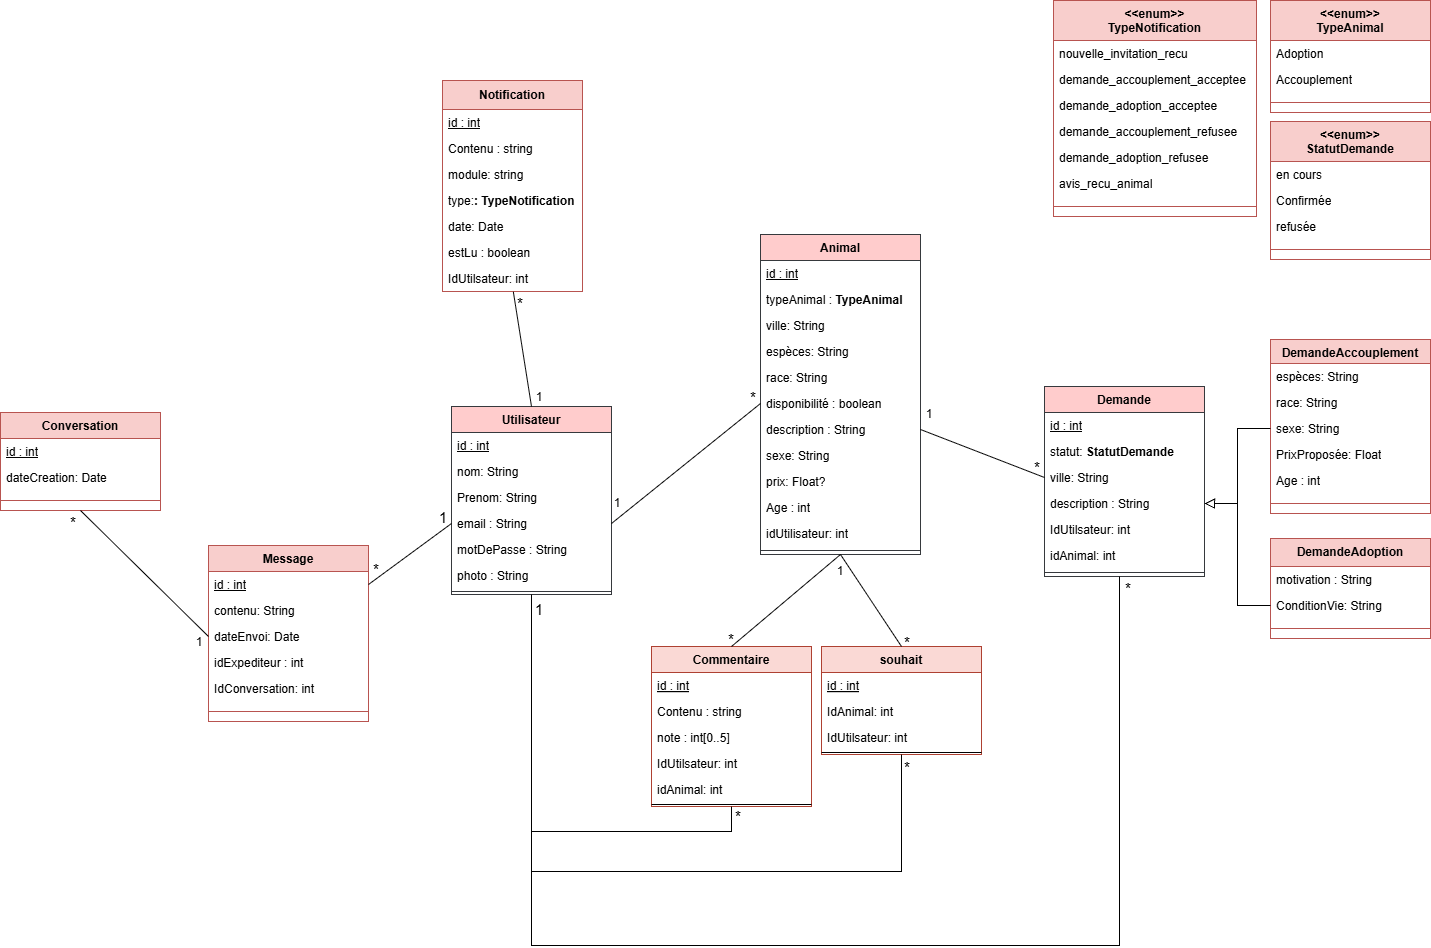
\includegraphics[width=1\textwidth]{images/diagramme classes animatch.png}
    \caption{Diagramme de classes de la sprint 2}
    \label{fig:class_diagram_sprint2}
\end{figure}  


\subsection{Diagrammes de séquences du sprint 2} 
Cette section présente les diagrammes de séquences du deuxieme sprint, illustrant les interactions entre les différents composants du système. 
\subsubsection{Diagramme de séquence : Gérer mes animaux pour accouplement et pour adoption}

Cette figure \ref{fig:gerer_animaux_animatch_seq} illustre les différentes interactions permettant à l’utilisateur de gérer ses animaux destinés à l’accouplement ou à l’adoption.

\newpage
\begin{figure}[H]
    \centering
    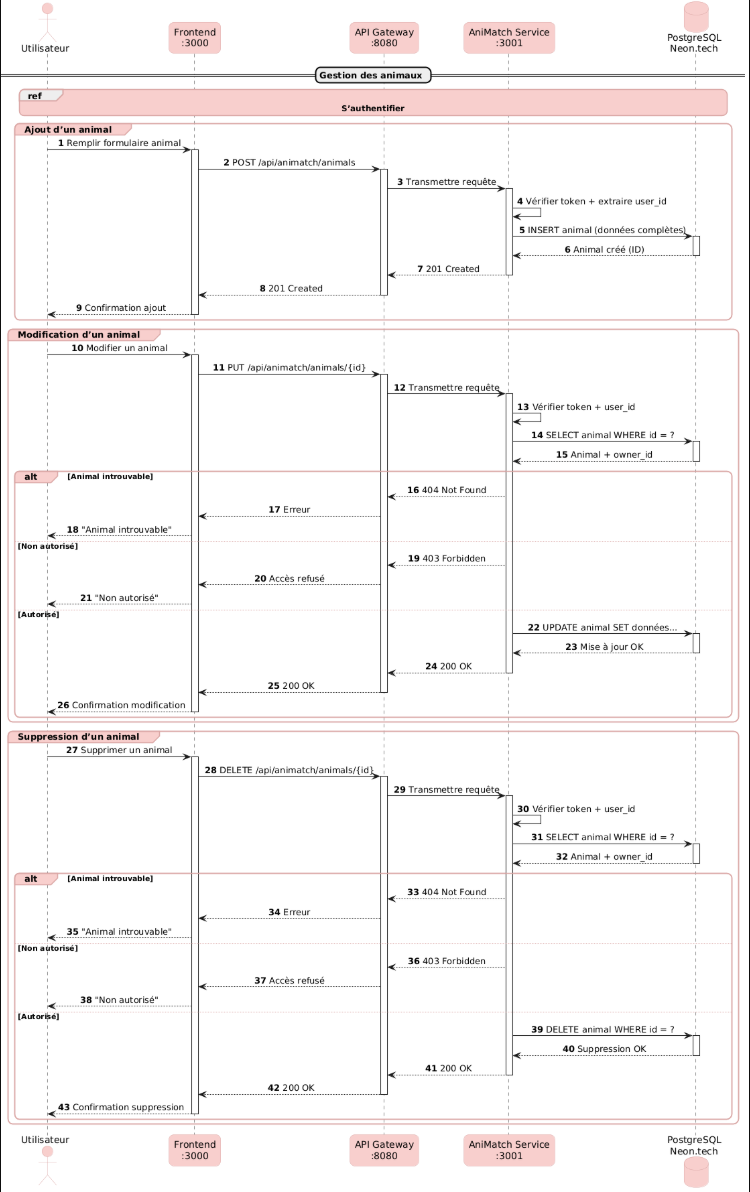
\includegraphics[width=0.75\textwidth]{images/gerer mes animaux animatch sq.png}
    \caption{Diagramme de séquence : gérer mes animaux pour accouplement et pour adoption}
    \label{fig:gerer_animaux_animatch_seq}
\end{figure}
\newpage 
\subsubsection{Diagramme de séquence : gérer mes invitations reçues}

Cette figure \ref{fig:gerer_invitations_recues_seq} illustre les interactions entre les composants du système lors de la gestion des invitations reçues. L’utilisateur peut consulter une invitation puis l’accepter ou la refuser. Le système met ensuite à jour son statut et envoie une notification aux utilisateurs concernés.

\begin{figure}[H]
    \centering
    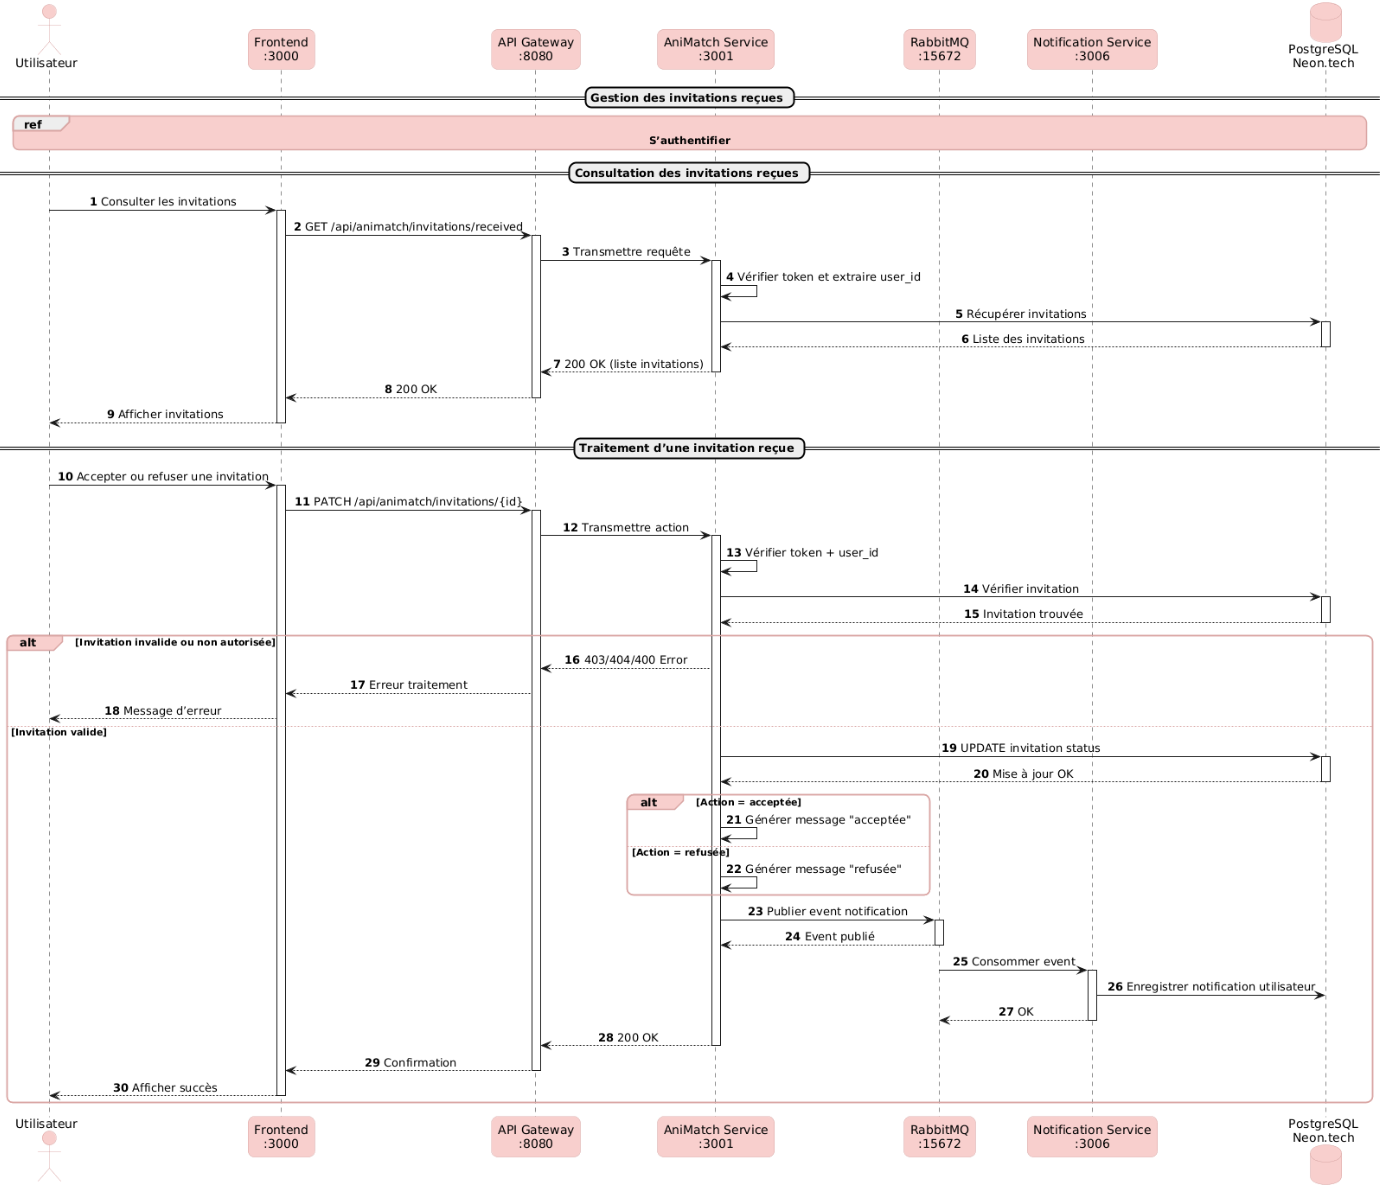
\includegraphics[width=1\textwidth]{images/gerer inv recus sq.png}
    \caption{Diagramme de séquence : gérer mes invitations reçues}
    \label{fig:gerer_invitations_recues_seq}
\end{figure}
\newpage 
\subsubsection{Diagramme de séquence : gérer mes invitations envoyées}

Cette figure \ref{fig:gerer_invitations_envoyees_seq} illustre les interactions entre les composants du système lors de la gestion des invitations envoyées. L’utilisateur peut consulter les invitations qu’il a envoyées et suivre leur état. Le système assure également la mise à jour des informations et l’envoi des notifications aux utilisateurs concernés.

\begin{figure}[H]
    \centering
    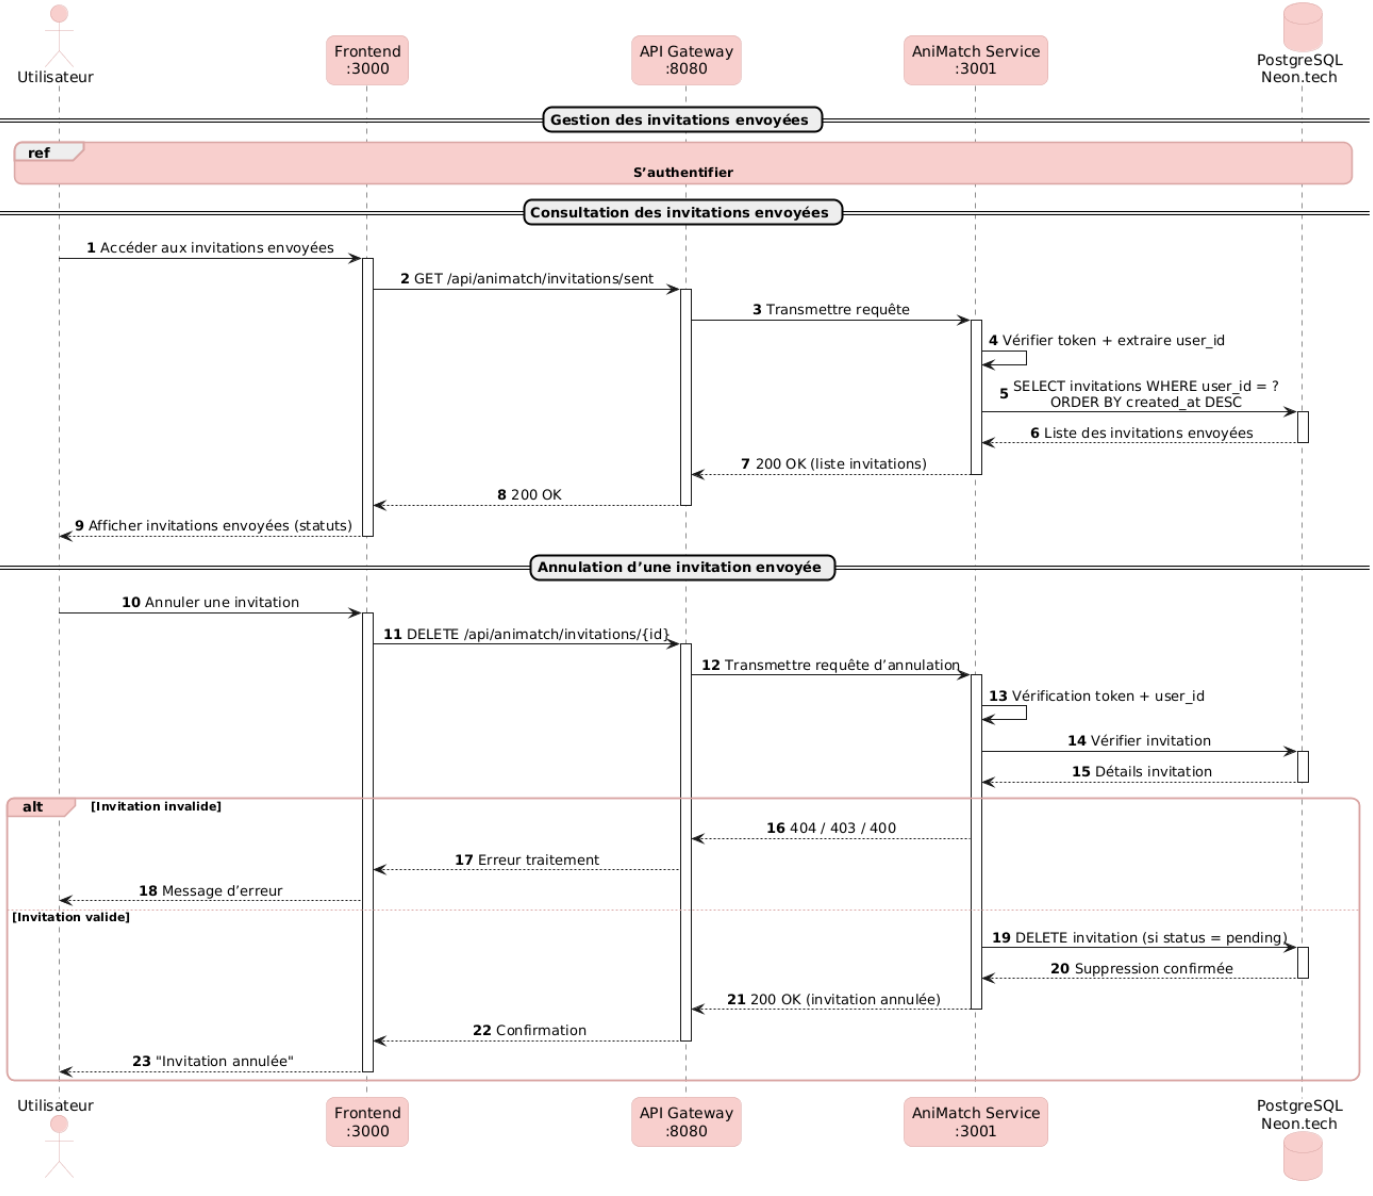
\includegraphics[width=1\textwidth]{images/gerer inv envoyes sq.png}
    \caption{Diagramme de séquence : gérer mes invitations envoyées}
    \label{fig:gerer_invitations_envoyees_seq}
\end{figure}

\newpage
\subsection{Réalisation du sprint 2} 

Dans cette partie, nous allons présenter les différentes interfaces graphiques de l’application développée, en lien avec les cas d’utilisation de cette sprint . 
\subsubsection{Interfaces d’accueil et menu principal de l’application AniHub}

Les figures \ref{fig:acceuil_anihub} et \ref{fig:menu_anihub} illustrent respectivement l’interface d’accueil de l’application AniHub et le menu principal permettant d’accéder aux différents modules de la plateforme.

\begin{figure}[h!]
    \centering
    
    \begin{minipage}{0.48\textwidth}
        \centering
        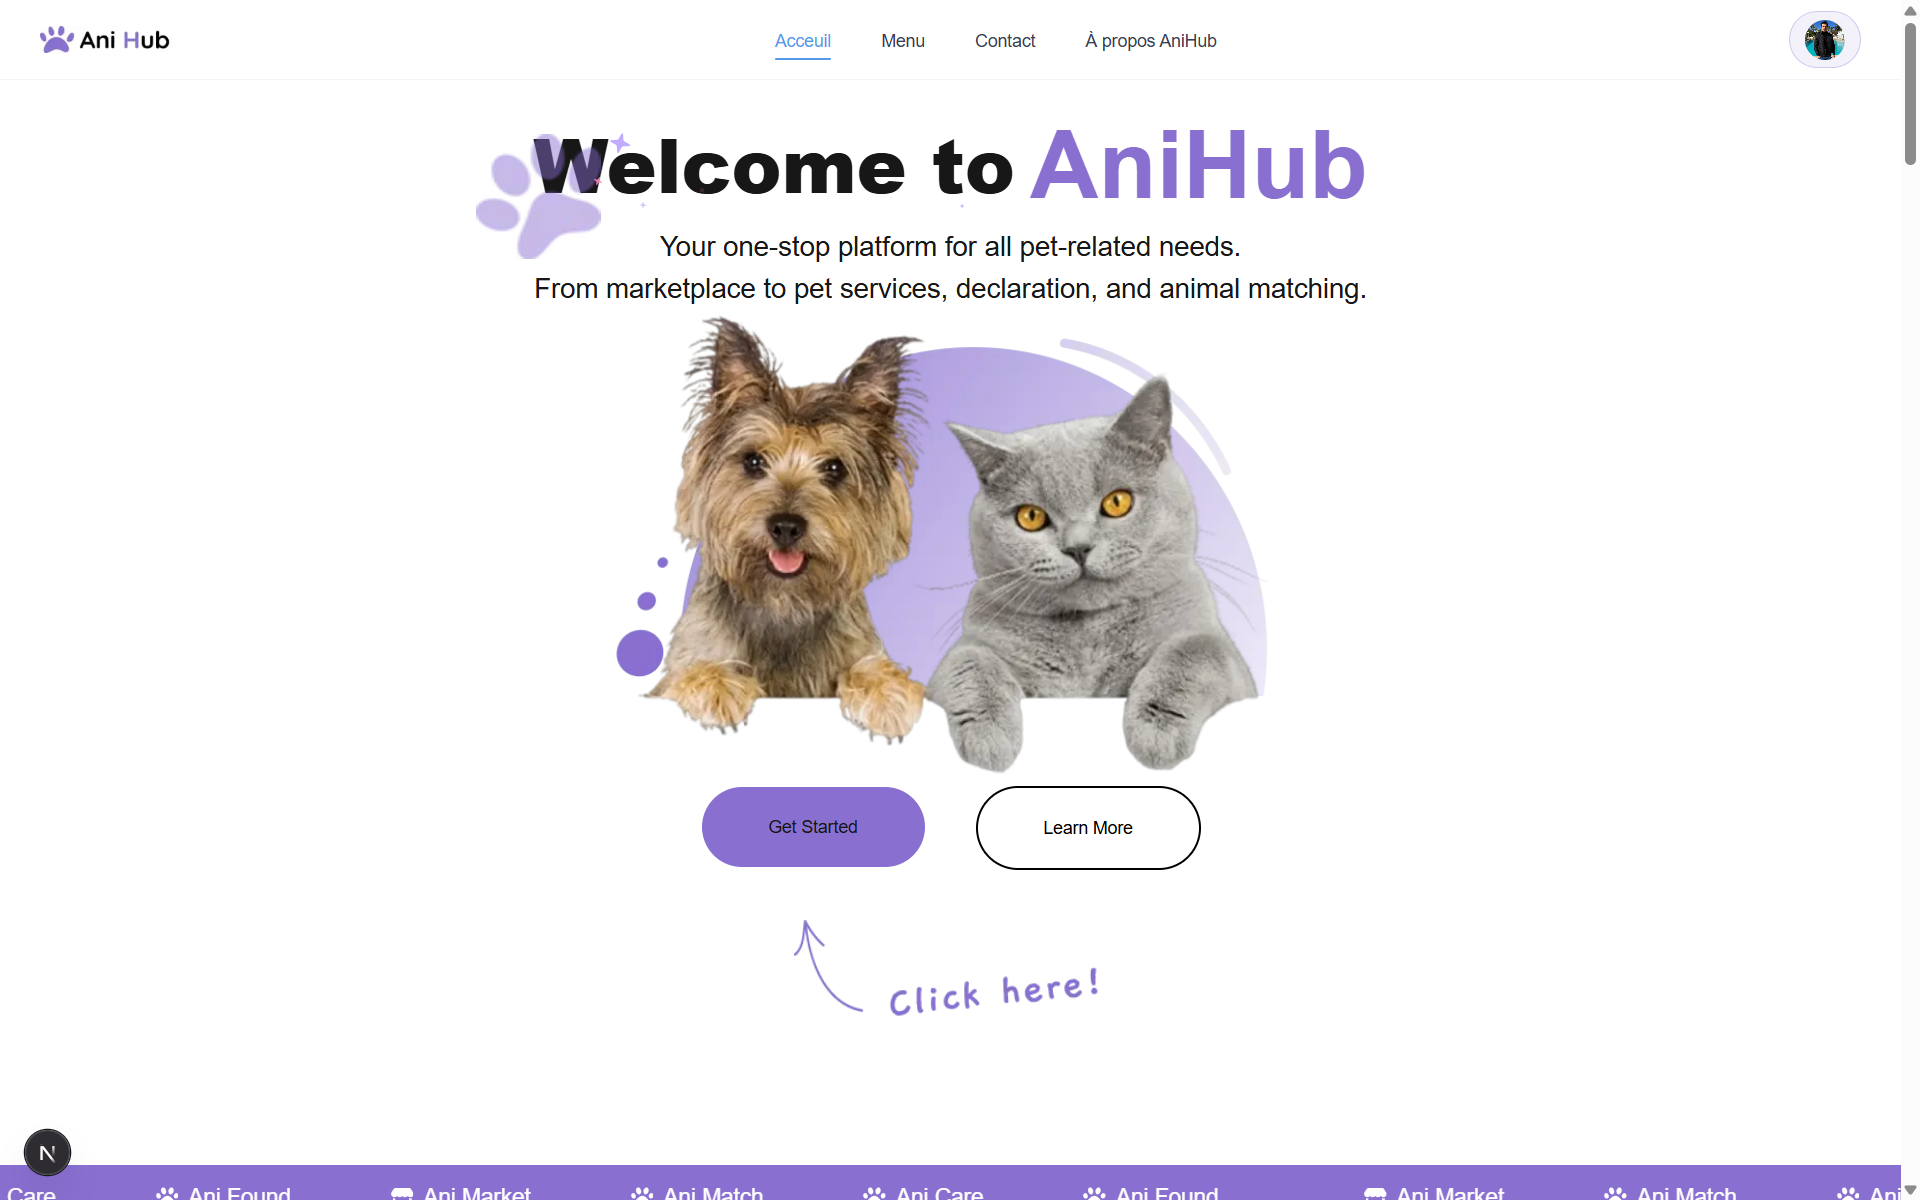
\includegraphics[width=\textwidth]{images/acceuil.png}
        \caption{Interface d’accueil AniHub}
        \label{fig:acceuil_anihub}
    \end{minipage}
    \hfill
    \begin{minipage}{0.48\textwidth}
        \centering
        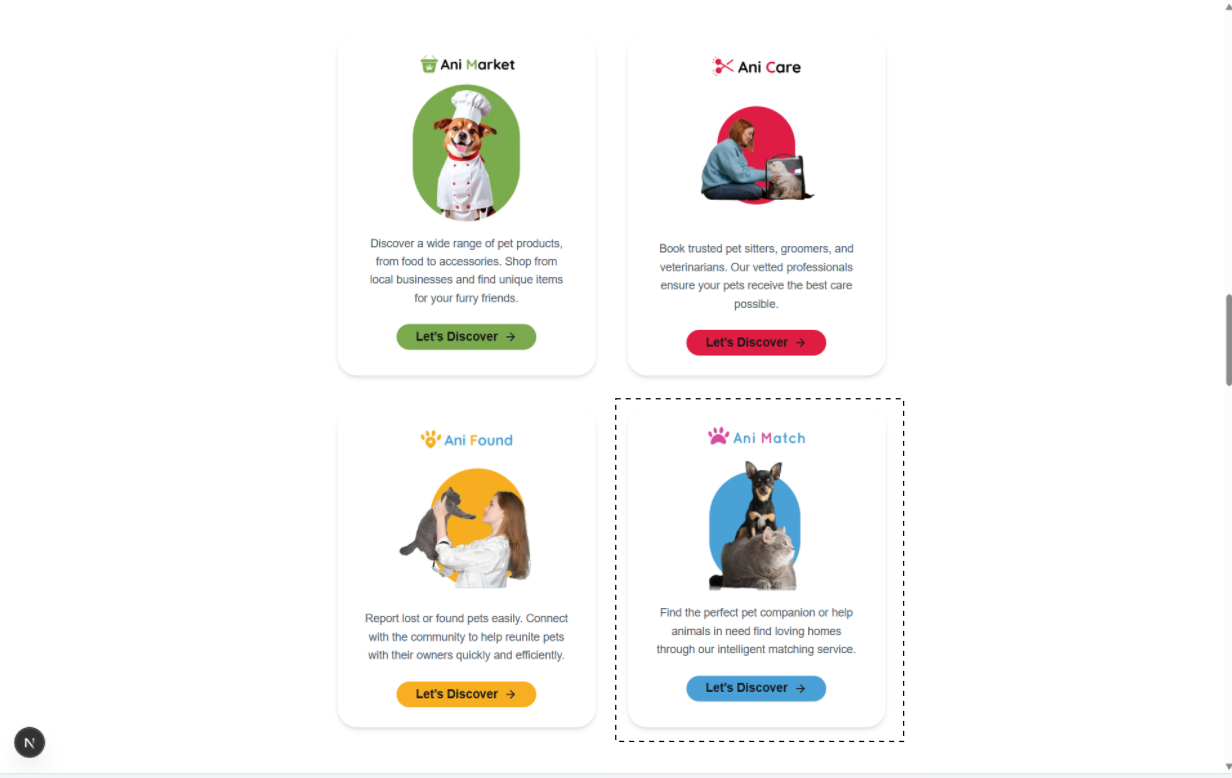
\includegraphics[width=\textwidth]{images/menu.png}
        \caption{Menu principal AniHub}
        \label{fig:menu_anihub}
    \end{minipage}

\end{figure} 

\subsubsection{Interface d’accueil AniMatch}

La figure \ref{fig:acceuil_animatch} illustre l’interface d’accueil du module AniMatch :

\begin{figure}[h!]
    \centering
    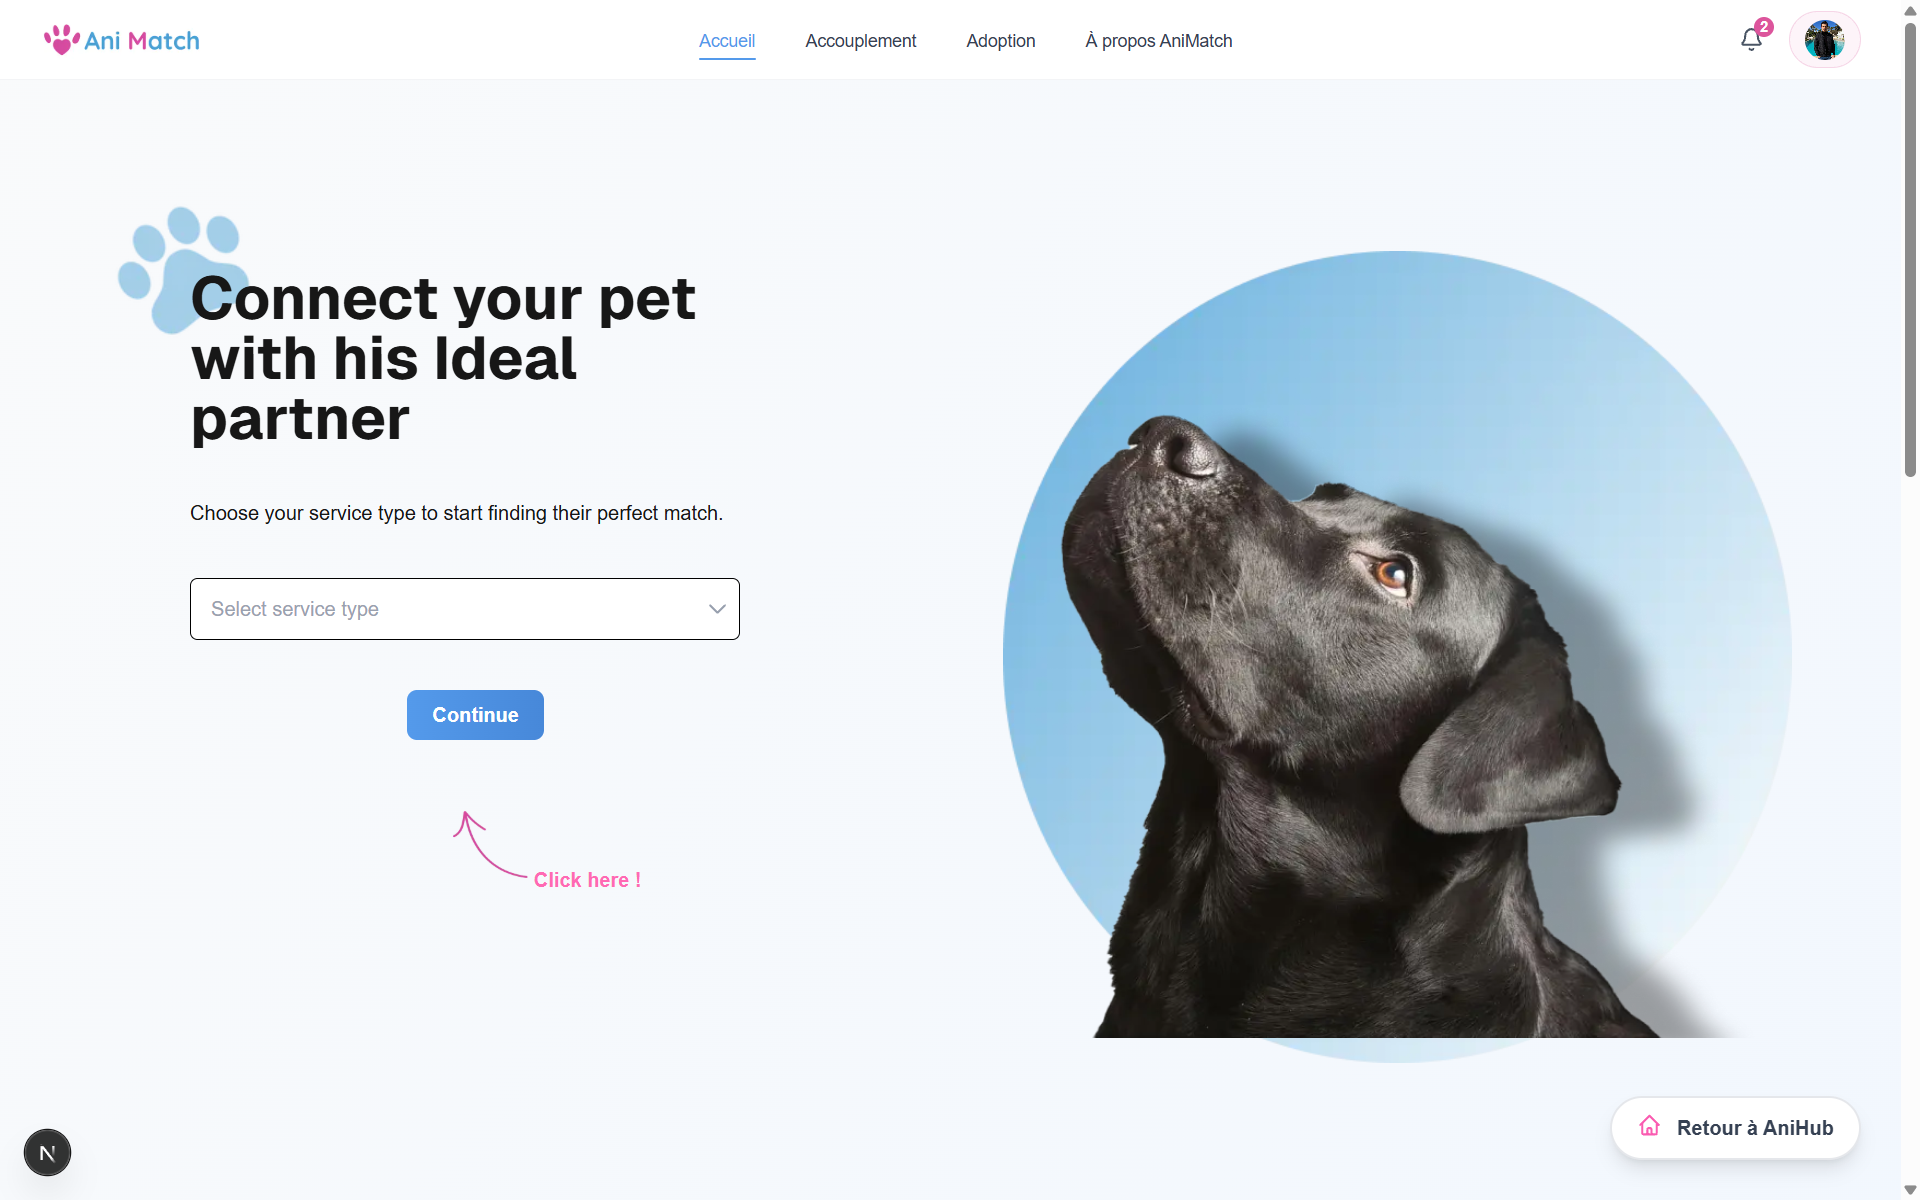
\includegraphics[width=0.8\textwidth]{images/acceuil animatch.png}
    \caption{Interface d’accueil du module AniMatch}
    \label{fig:acceuil_animatch}
\end{figure}   

\newpage

\subsubsection{Interface d’ajout d’une annonce d’accouplement}

La figure \ref{fig:ajout_annonce_accouplement} illustre l’interface permettant d’ajouter une annonce d’accouplement.

\begin{figure}[h!]
    \centering
    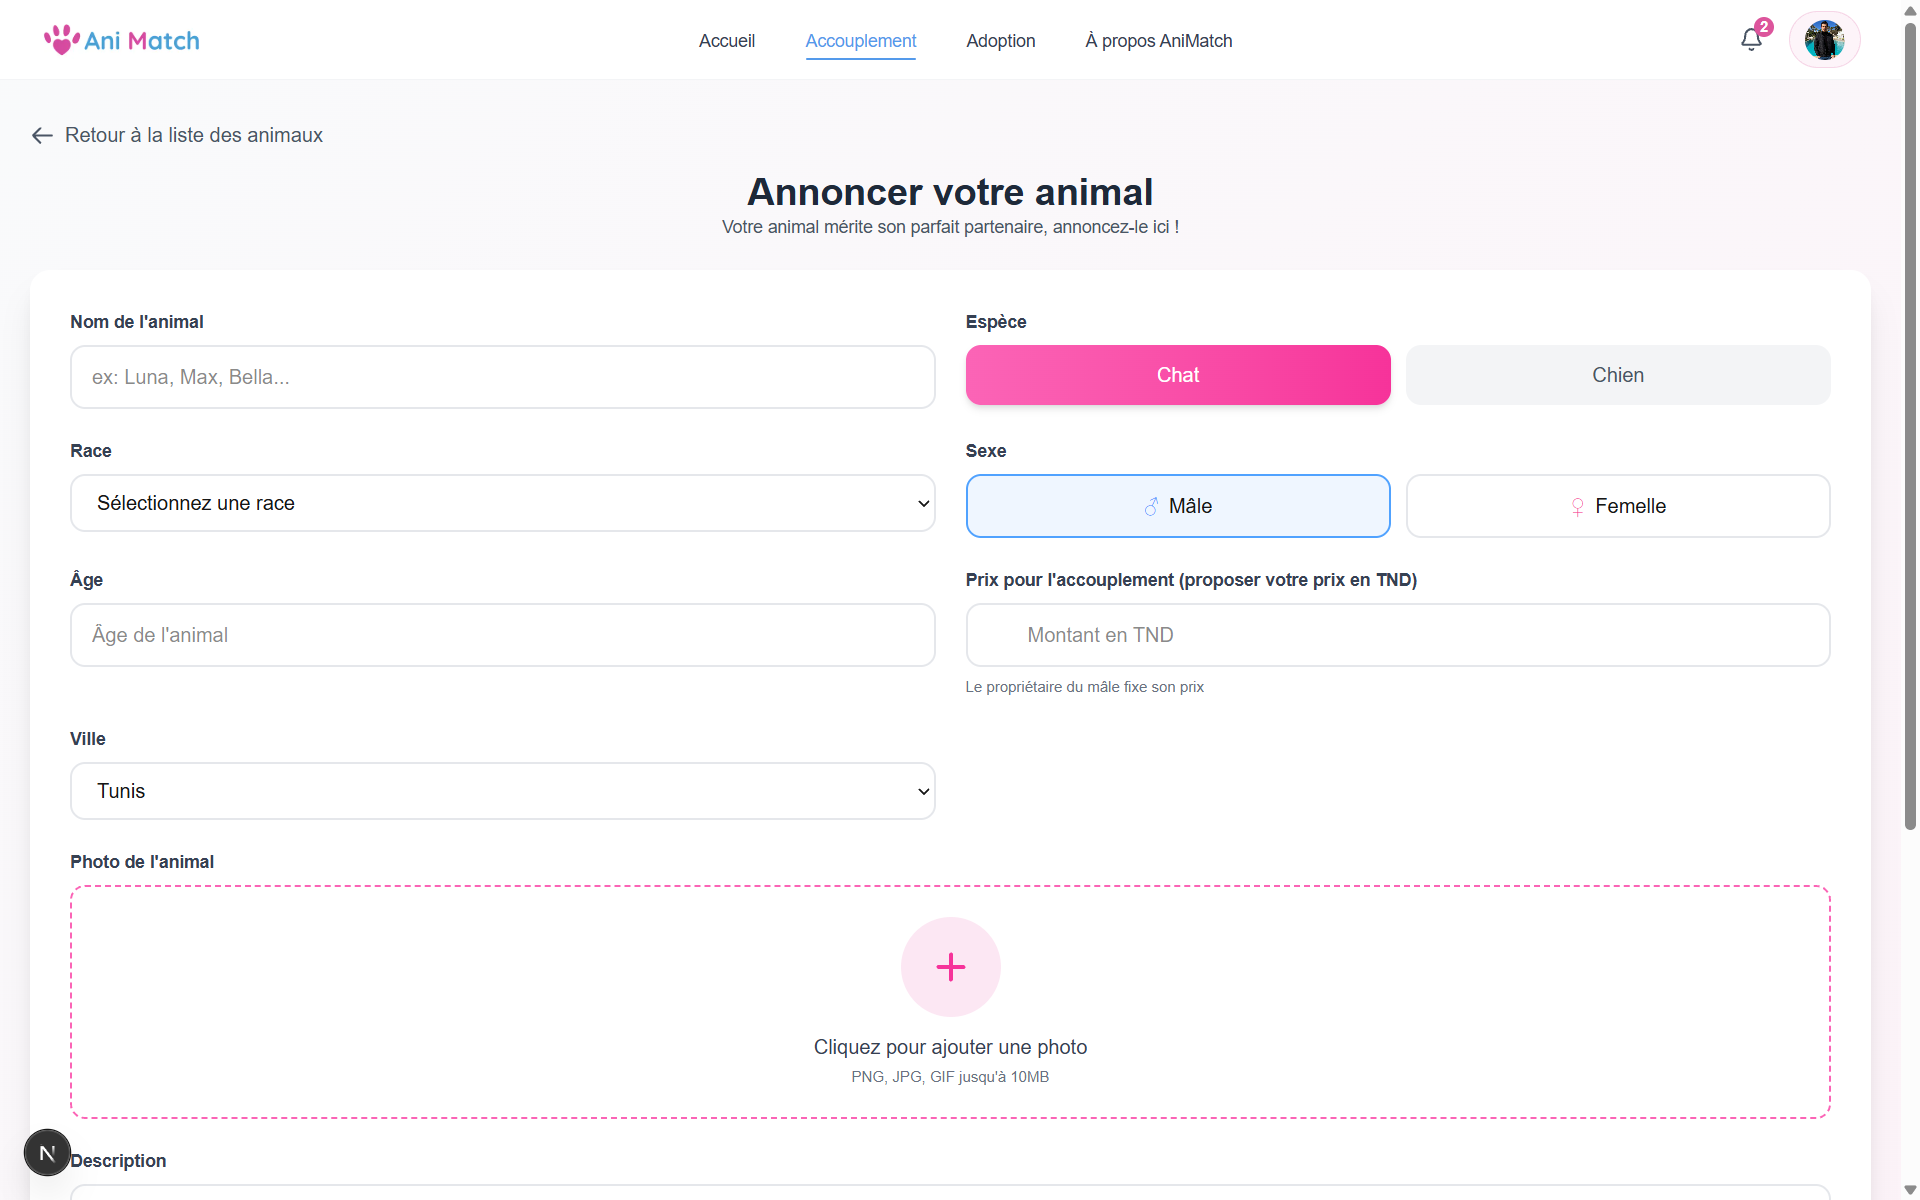
\includegraphics[width=0.74\textwidth]{images/ajouter animal accouplemnt.png}
    \caption{Interface d’ajout d’une annonce d’accouplement}
    \label{fig:ajout_annonce_accouplement}
\end{figure}

\subsubsection{Interface des animaux pour accouplement}

La figure \ref{fig:animaux_accouplement} illustre la liste des animaux disponibles pour l’accouplement.

\begin{figure}[h!]
    \centering
    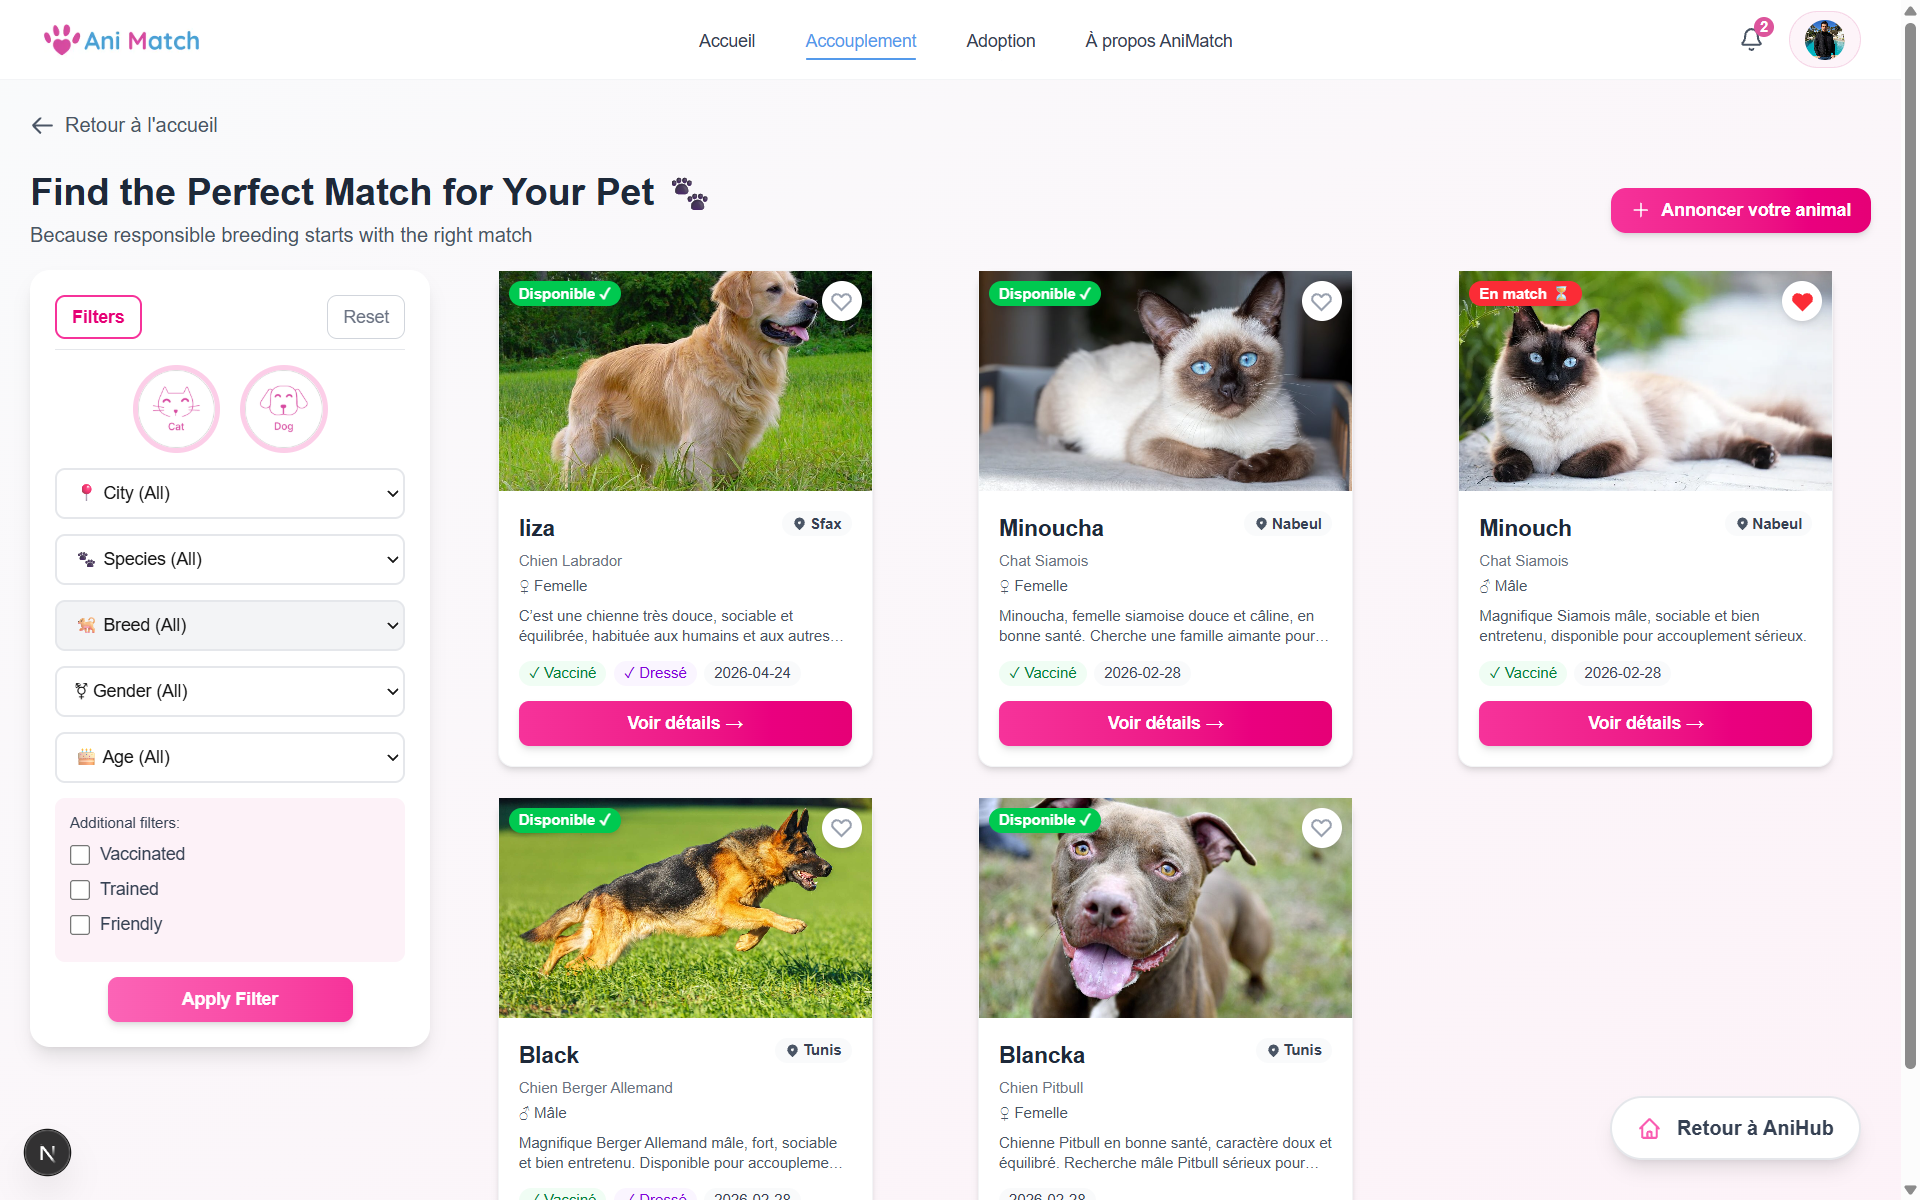
\includegraphics[width=0.74\textwidth]{images/animals accouplement.png}
    \caption{Interface des animaux pour accouplement}
    \label{fig:animaux_accouplement}
\end{figure}  

\newpage 

\subsubsection{Interface de détails d’une annonce d’accouplement}

La figure \ref{fig:details_annonce_accouplement} illustre les détails d’une annonce d’accouplement.

\begin{figure}[h!]
    \centering
    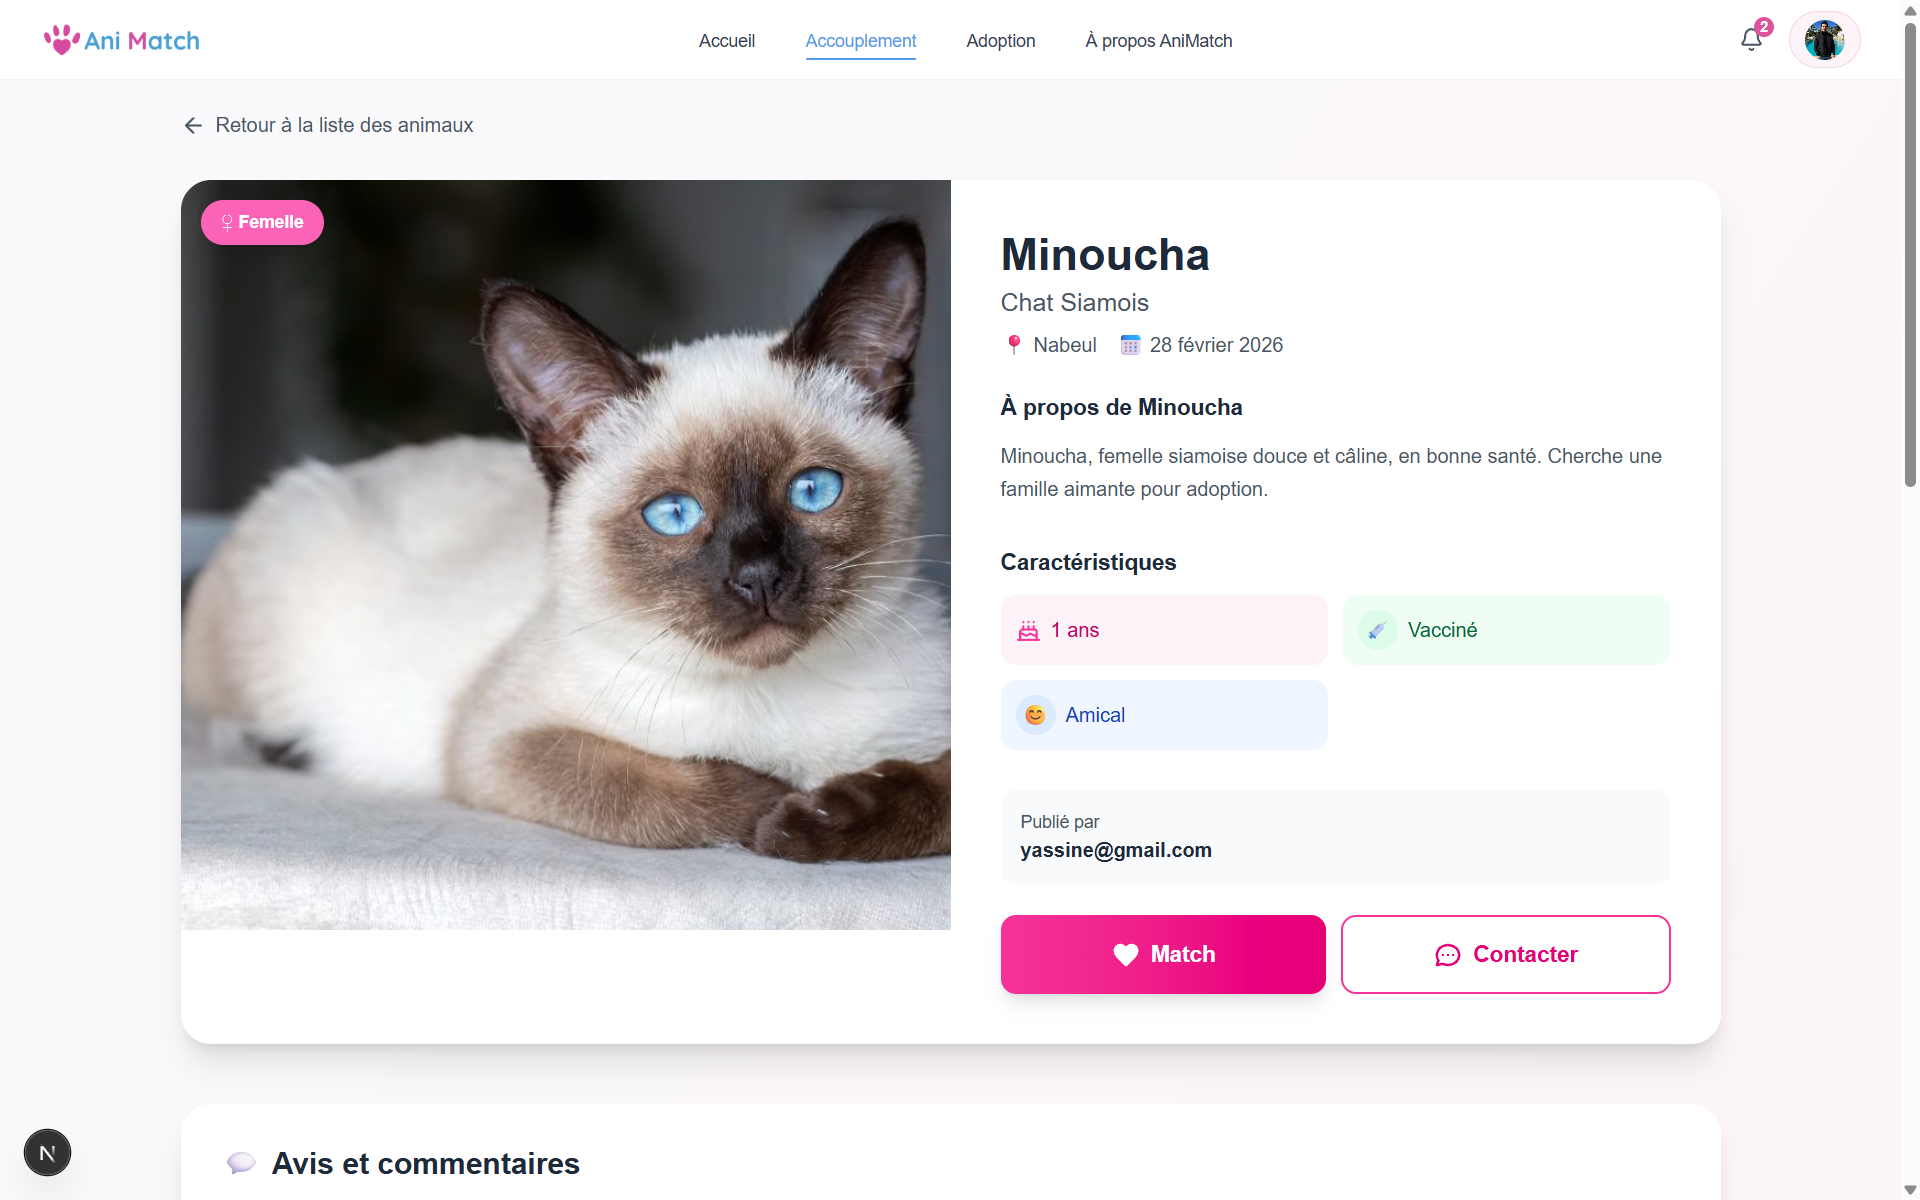
\includegraphics[width=0.72\textwidth]{images/detail.png}
    \caption{Interface de détails d’une annonce d’accouplement}
    \label{fig:details_annonce_accouplement}
\end{figure}

\subsubsection{Interface d’envoi d’une invitation d’accouplement}

La figure \ref{fig:envoyer_invitation_accouplement} illustre l’interface d’envoi d’une invitation à l’accouplement, permettant à l’utilisateur de rédiger un message et de l’envoyer au propriétaire de l’annonce.
\begin{figure}[h!]
    \centering
    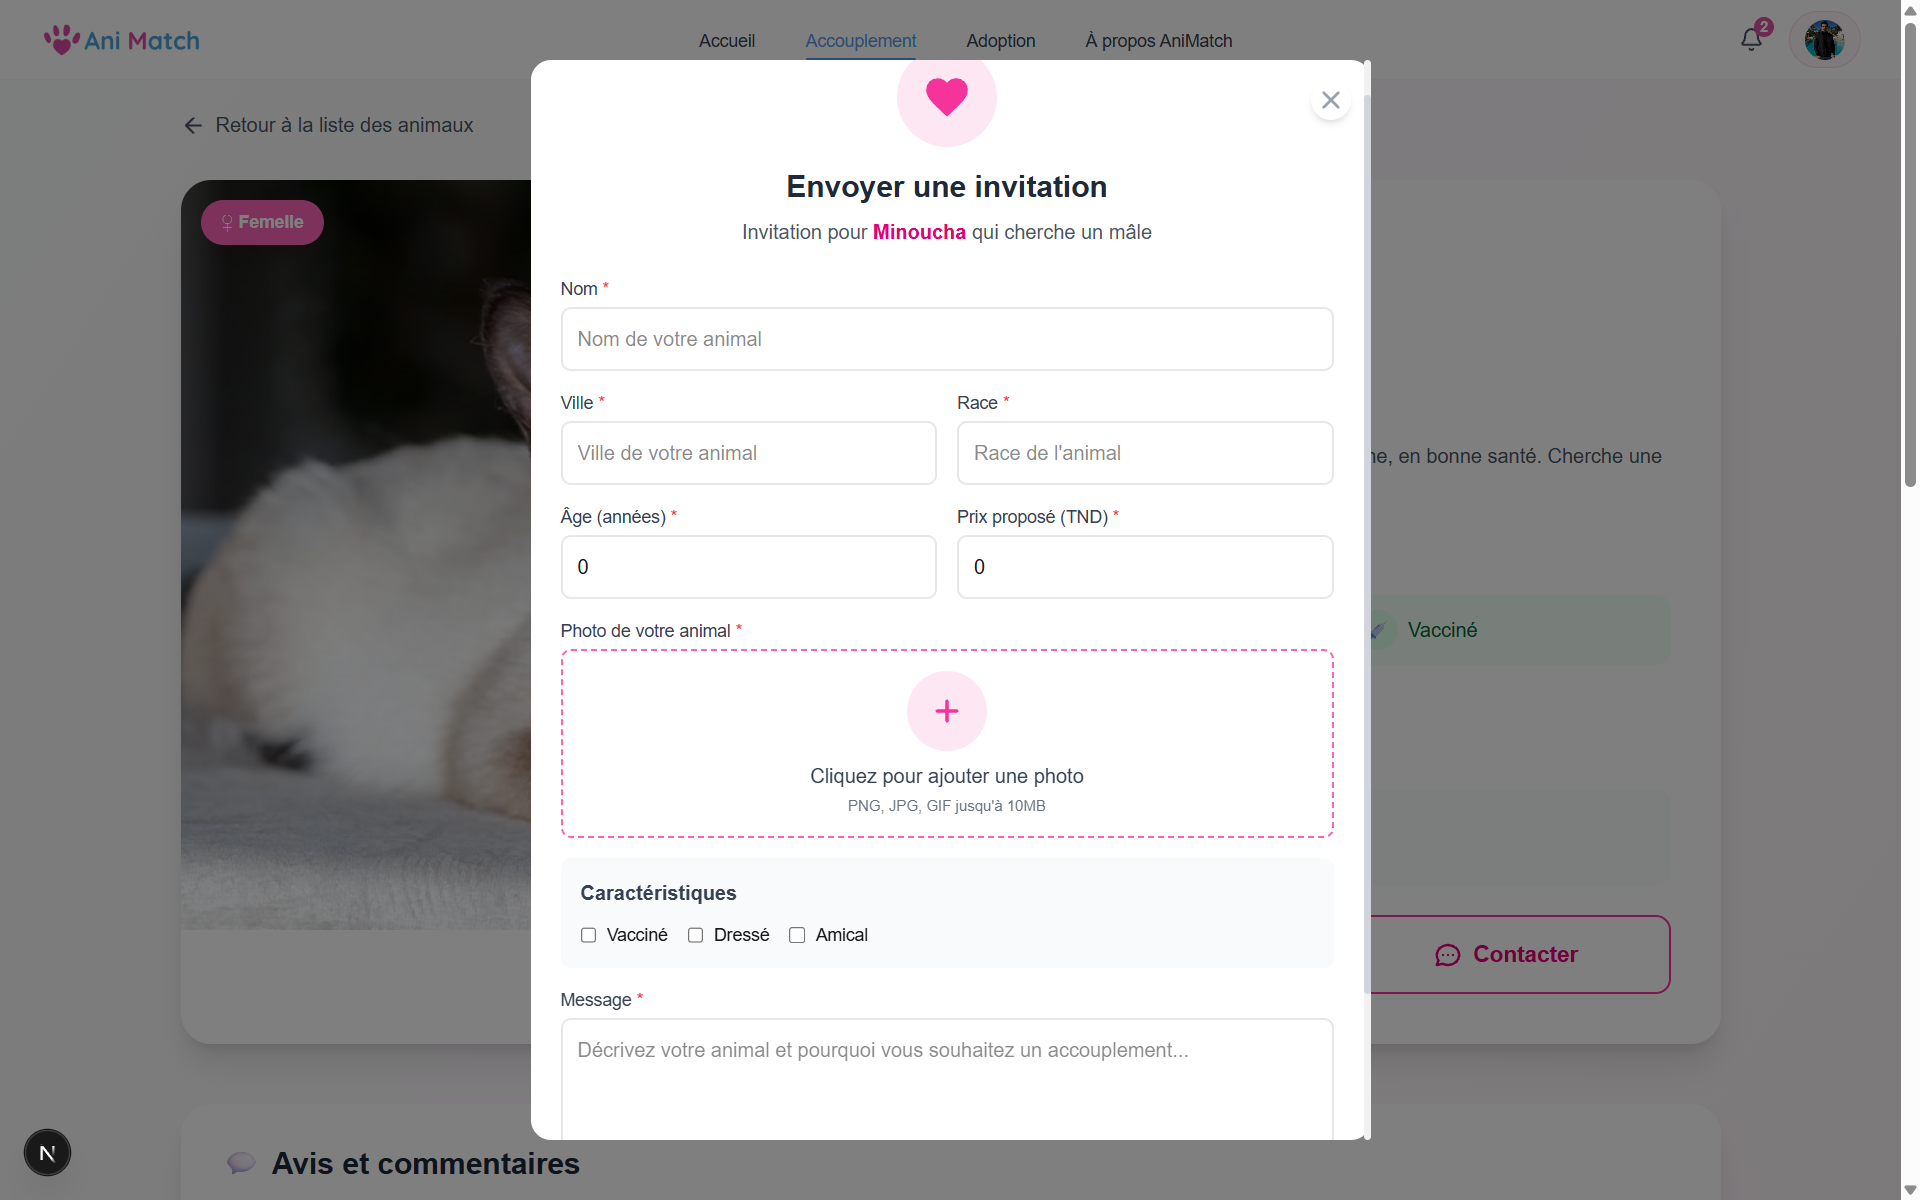
\includegraphics[width=0.72\textwidth]{images/envoyer invitation.png}
    \caption{Interface d’envoi d’une invitation à l’accouplement}
    \label{fig:envoyer_invitation_accouplement}
\end{figure} 

\newpage

\subsubsection{Interface des avis et commentaires}

La figure \ref{fig:avis_commentaires} illustre l’interface des avis et commentaires.

\begin{figure}[h!]
    \centering
    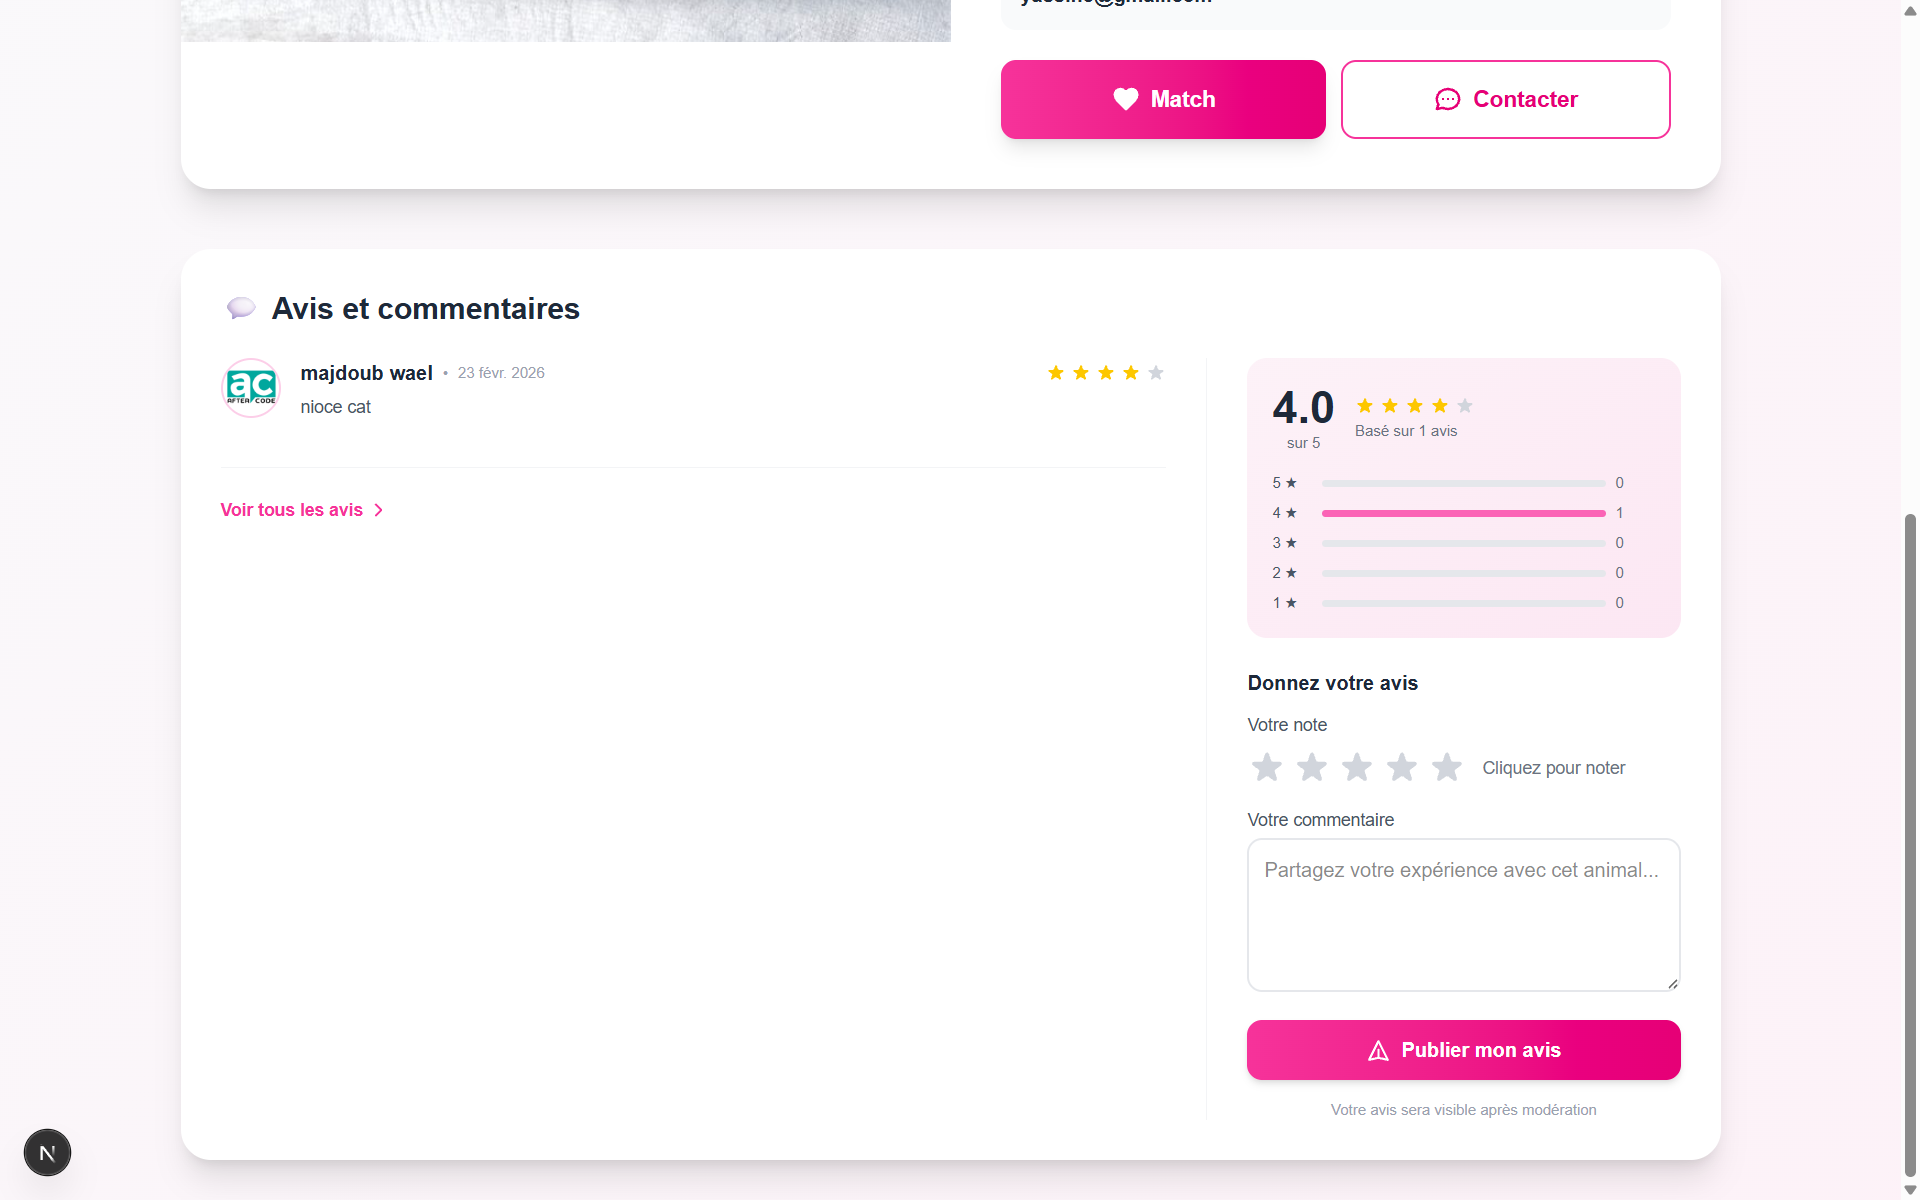
\includegraphics[width=0.74\textwidth]{images/comments section.png}
    \caption{Interface des avis et commentaires}
    \label{fig:avis_commentaires}
\end{figure} 

\subsubsection{Interface de gestion du profil}

La figure \ref{fig:gestion_profil} illustre l’interface de gestion du profil utilisateur dans son espace personnel « Espace AniMatch ». 
\begin{figure}[h!]
    \centering
    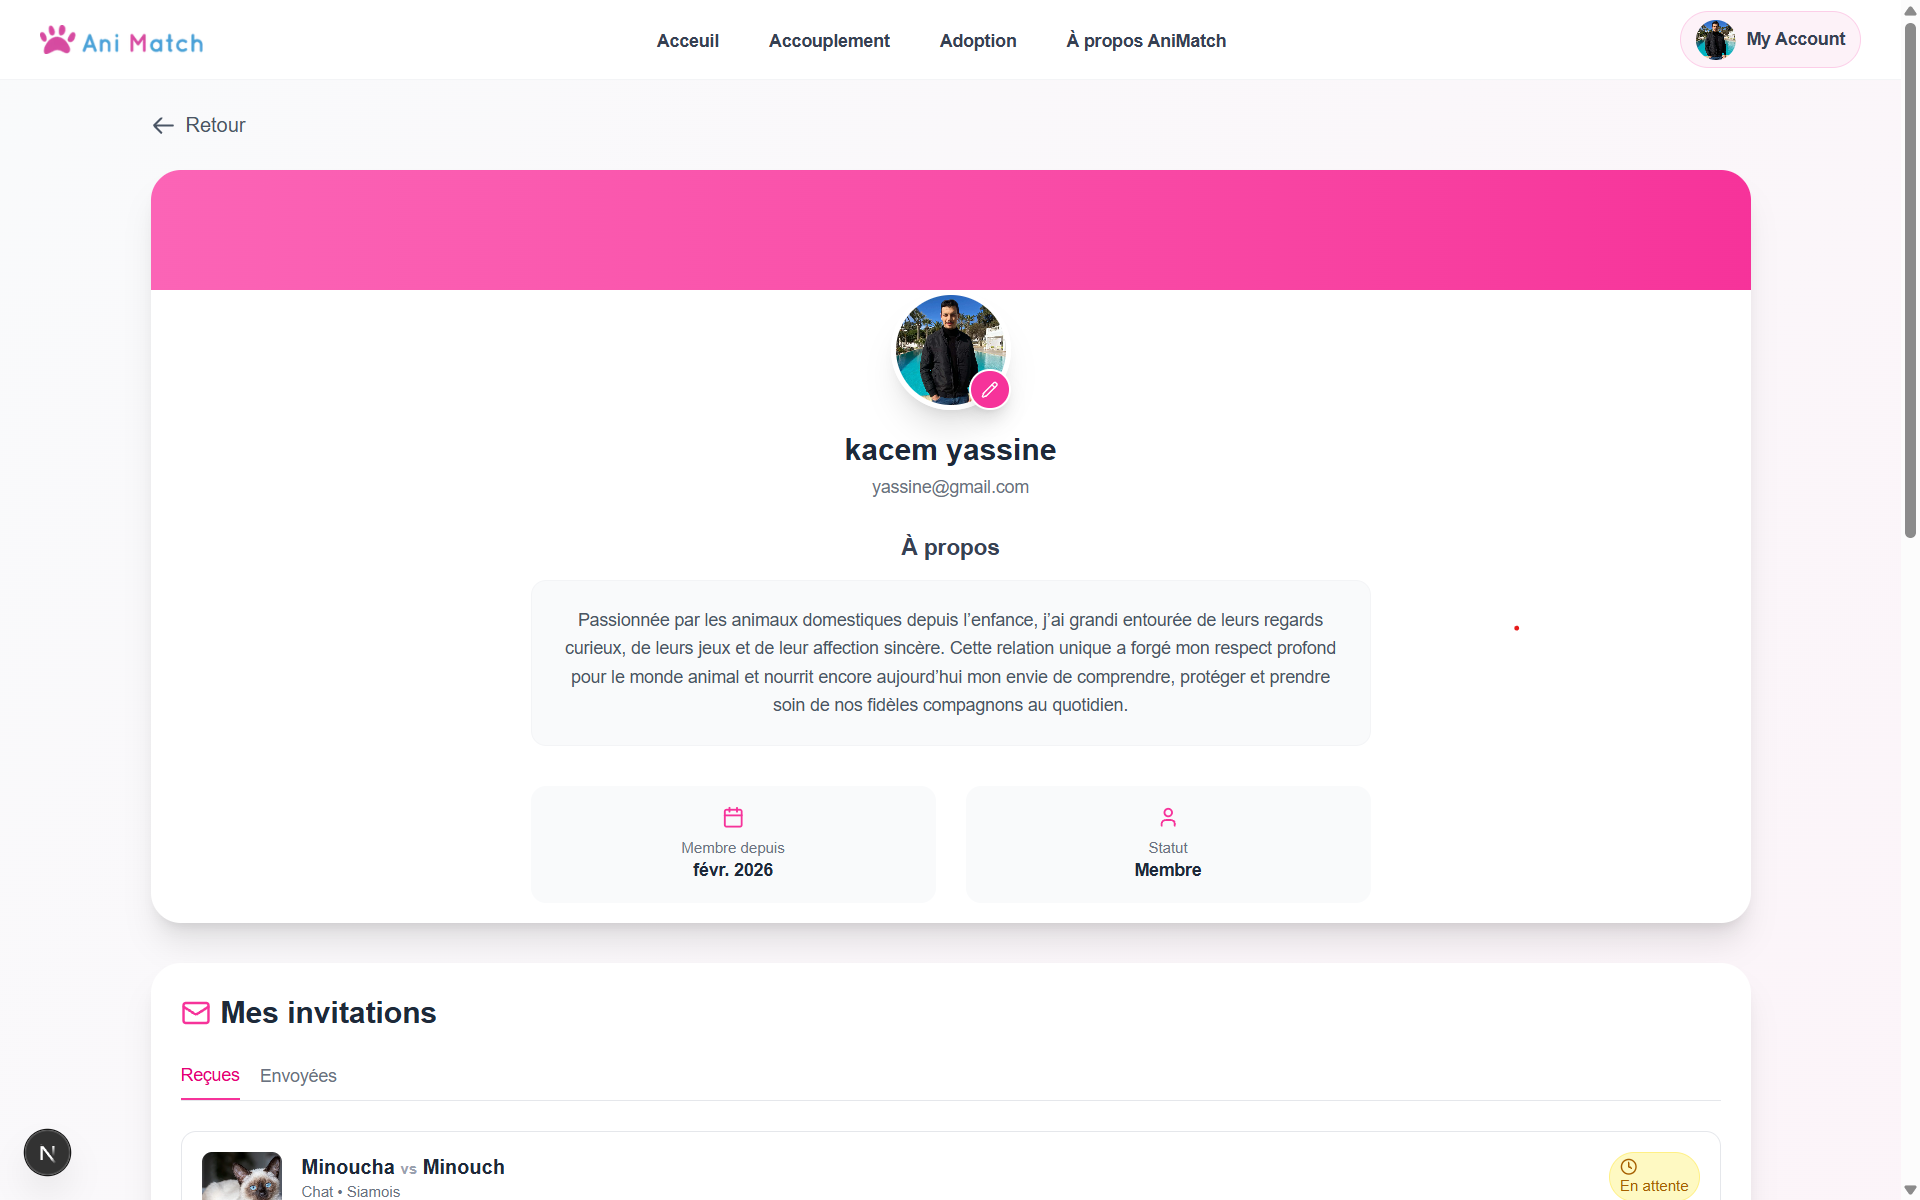
\includegraphics[width=0.74\textwidth]{images/profil page .png}
    \caption{Interface de gestion du profil utilisateur}
    \label{fig:gestion_profil}
\end{figure} 

\subsubsection{Interface de gestion de mes animaux (modification et suppression)} 

La figure \ref{fig:gestion_animaux_animatch} illustre l’interface de gestion des animaux permettant la modification et la suppression.

\begin{figure}[h!]
    \centering
    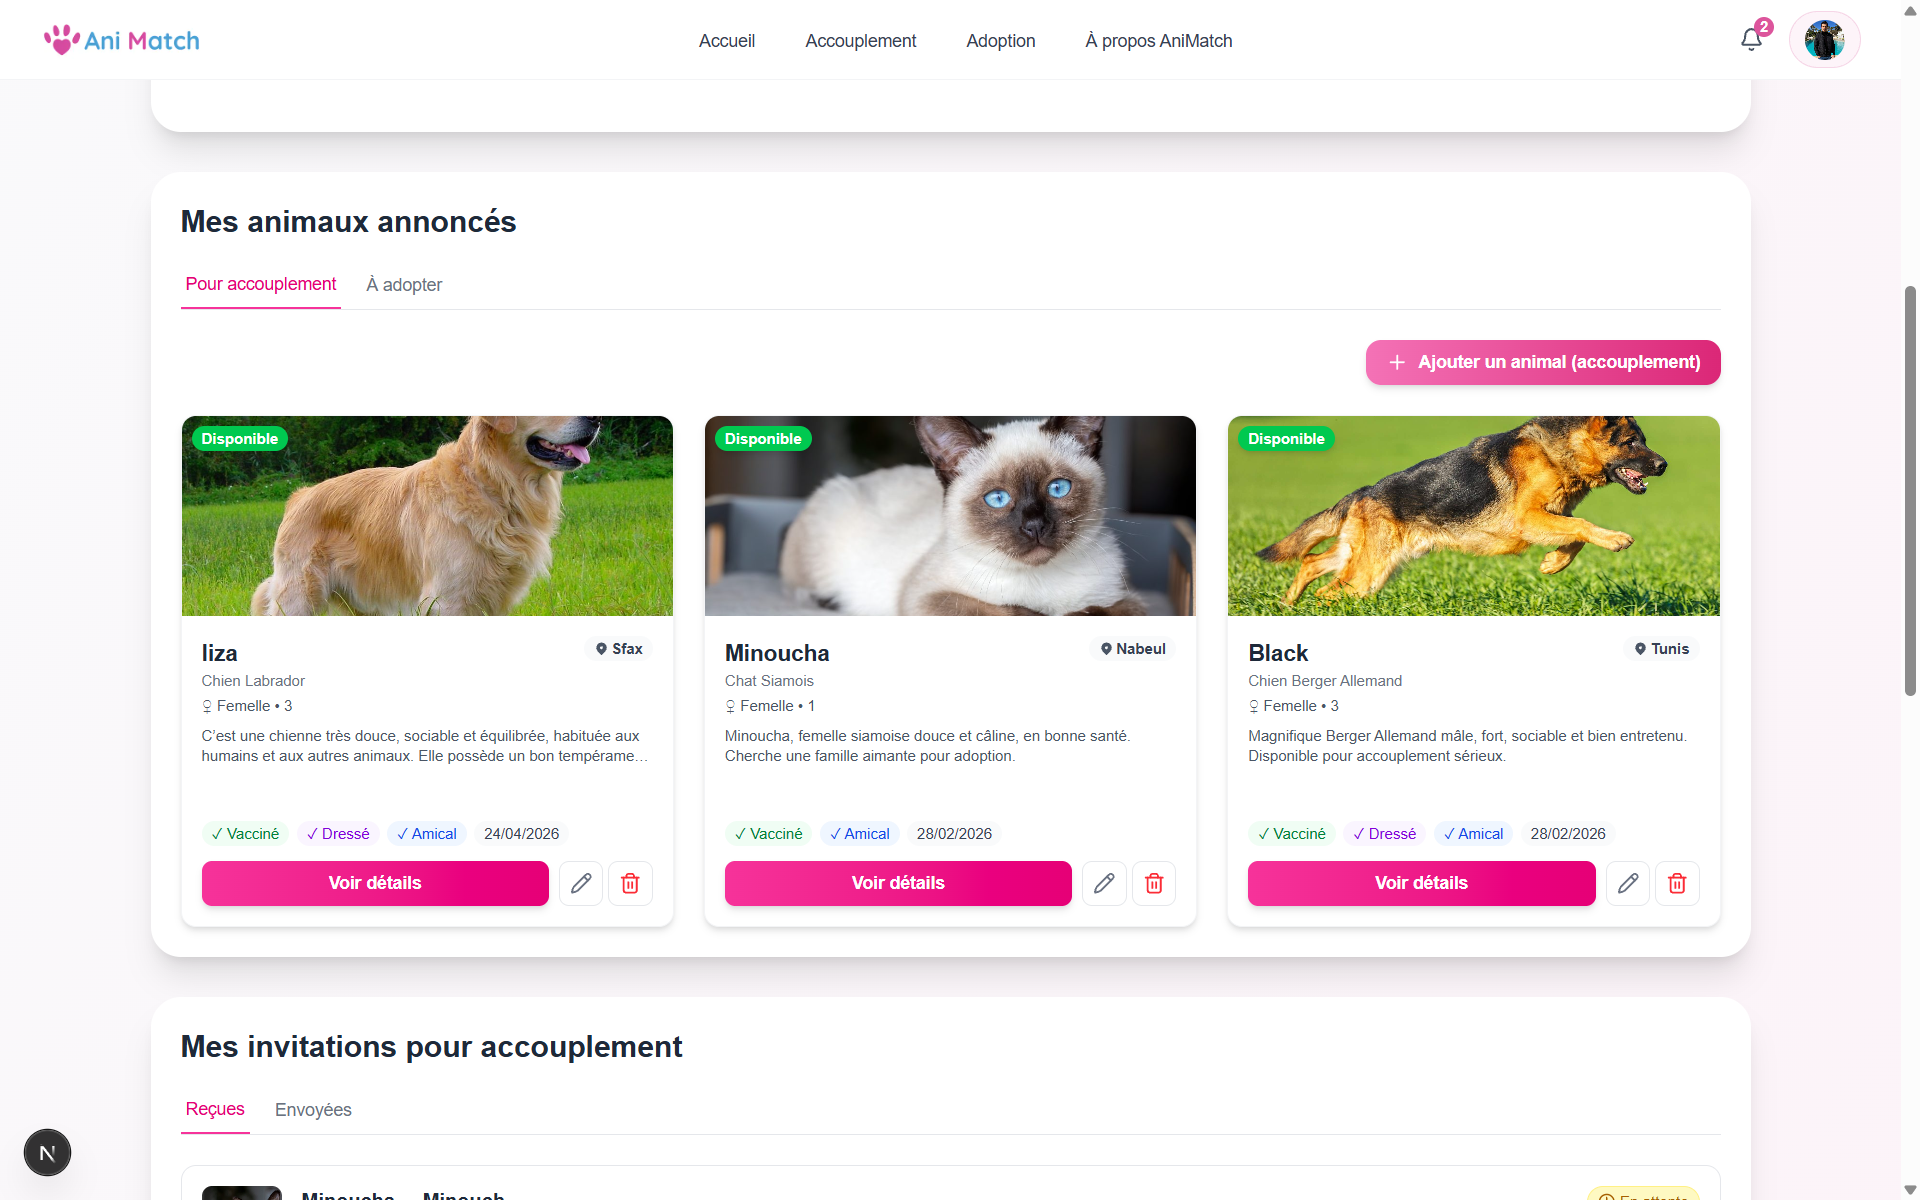
\includegraphics[width=0.74\textwidth]{images/profil page 2.png}
    \caption{Interface de gestion des animaux (modification et suppression)}
    \label{fig:gestion_animaux_animatch}
\end{figure}

\subsubsection{Interface de gestion de mes invitations pour adoption reçues} 

La figure \ref{fig:invitations_adoption_recues} illustre l’interface de gestion des invitations d’adoption reçues.

\begin{figure}[h!]
    \centering
    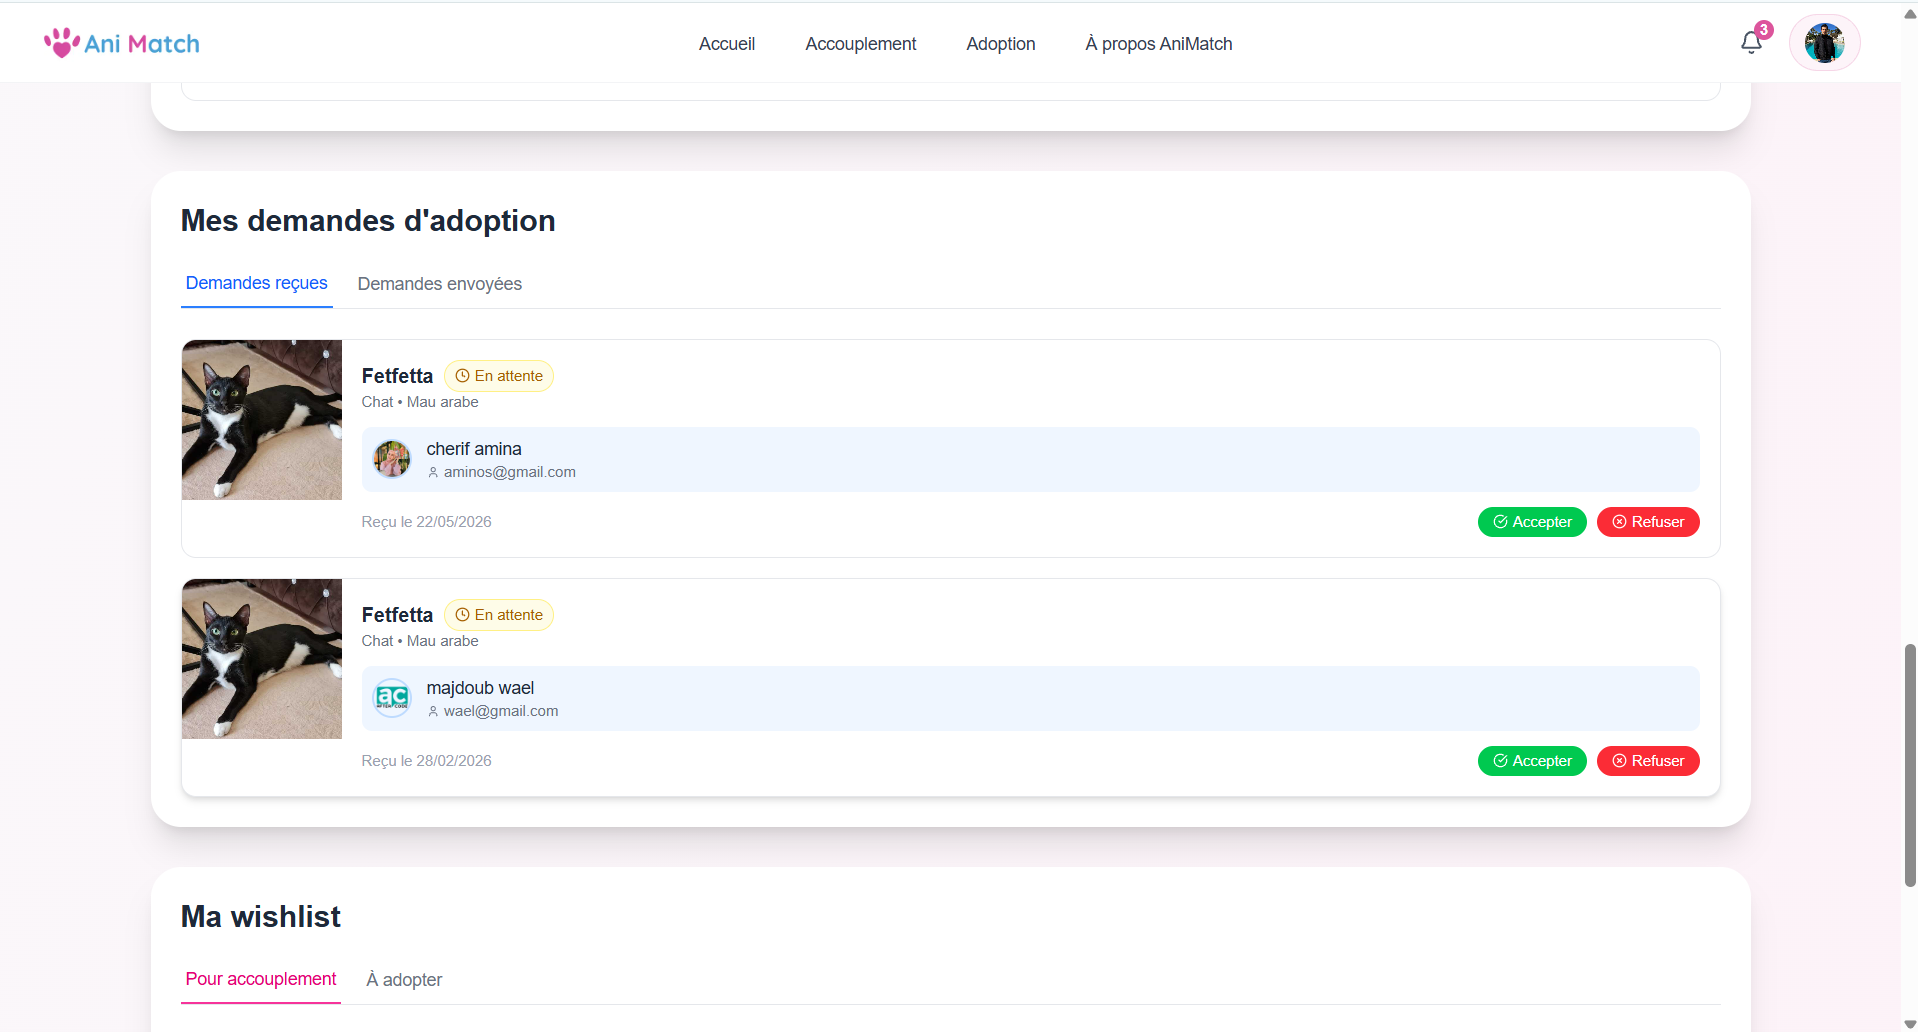
\includegraphics[width=0.85\textwidth]{images/mes demandes d adoption recus.png}
    \caption{Interface de gestion des invitations d’adoption reçues}
    \label{fig:invitations_adoption_recues}
\end{figure}

\newpage 

\subsubsection{Interface de gestion de mes invitations pour accouplement reçues}

La figure \ref{fig:invitations_accouplement_recues} illustre l’interface de gestion des invitations d’accouplement reçues.

\begin{figure}[h!]
    \centering
    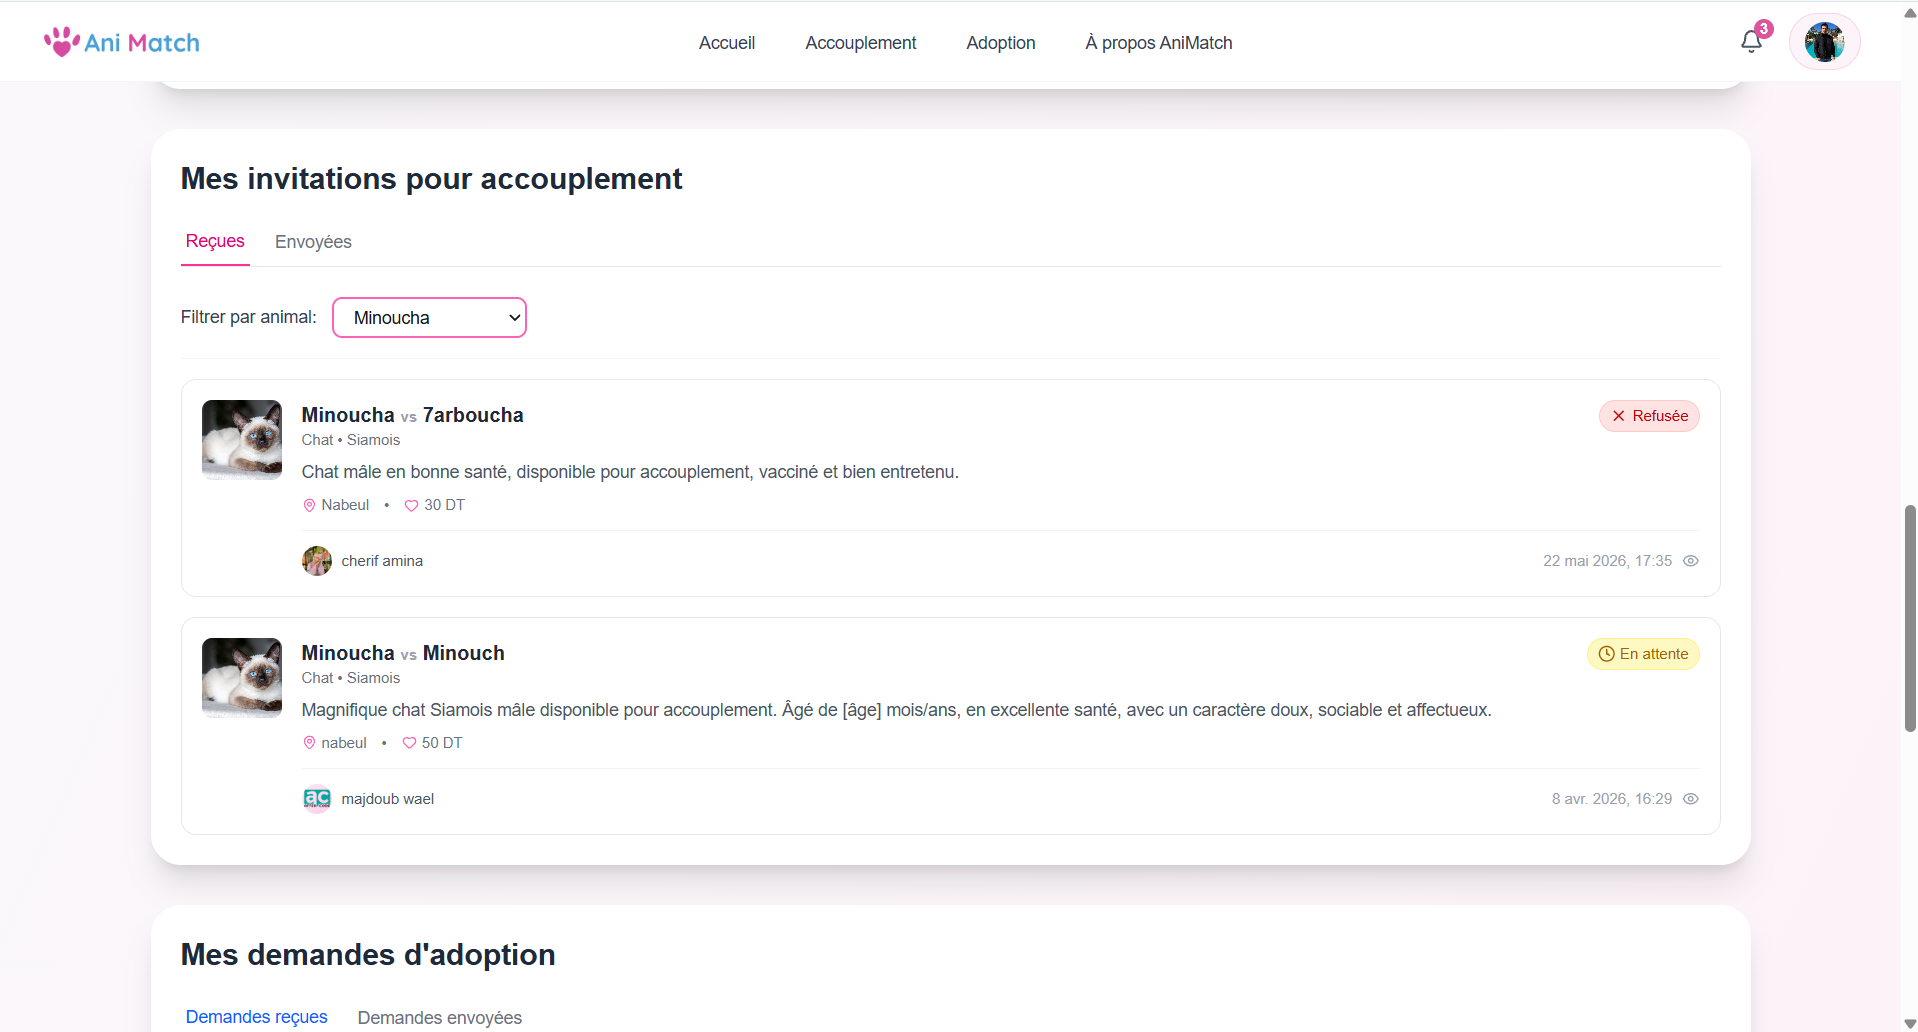
\includegraphics[width=0.85\textwidth]{images/mes invitations pour accouplements recus.png}
    \caption{Interface de gestion des invitations d’accouplement}
    \label{fig:invitations_accouplement_recues}
\end{figure} 

\subsubsection{Interface de détails d’une invitation d’accouplement reçue}

La figure \ref{fig:details_invitation_accouplement} illustre les détails d’une invitation d’accouplement reçue.

\begin{figure}[h!]
    \centering
    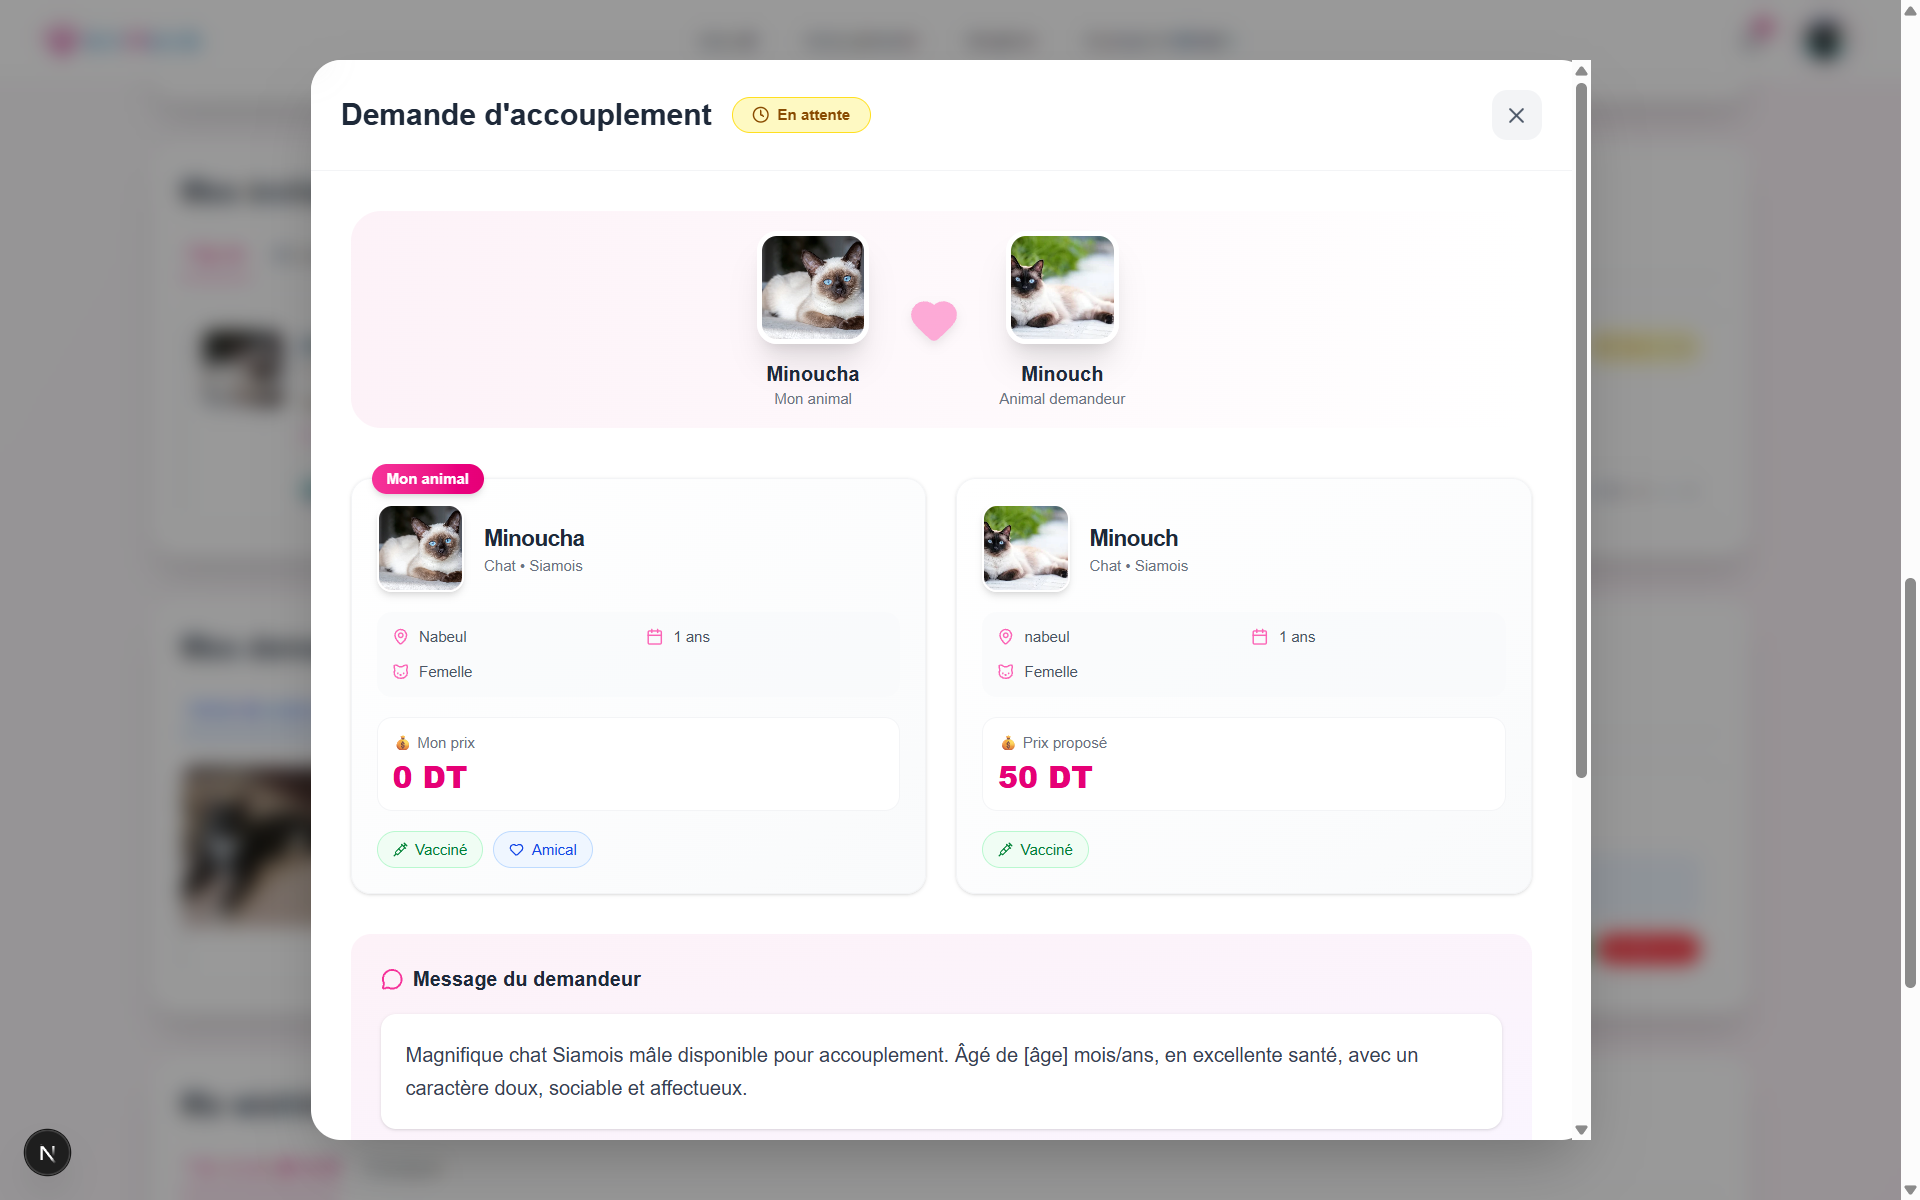
\includegraphics[width=0.8\textwidth]{images/invi recu 1.png}
    \caption{Interface de détails d’une invitation d’accouplement}
    \label{fig:details_invitation_accouplement}
\end{figure}

\newpage\section{Sprint 3 : Module AniFound}
La figure \ref{fig:logo-anifound} illustre le logo du module AniFound.

\begin{figure}[h!]
    \centering
    
\includegraphics[width=3.5cm]{images/Logo anifound.png}
    \caption{Logo du module AniFound}
    \label{fig:logo-anifound}
\end{figure}

Ce sprint de \textbf{3 semaines} est consacré au module AniFound, dédié à la déclaration et la gestion des animaux trouvés, ainsi qu’à leur restitution à leurs propriétaires.
\subsection{Sprint backlog}  
La table \ref{tab:sprint3-backlog} présente le Sprint Backlog du sprint 3 avec les user stories, les tâches associées et les efforts estimés :
\begin{longtable}{|p{2cm}|p{5cm}|p{6cm}|p{2cm}|}
\caption{Sprint Backlog du sprint 3 }
\label{tab:sprint3-backlog} \\ 
\hline
\rowcolor{coloranifound}
\textbf{ID} & \textbf{User Story} & \textbf{Tâches} & \textbf{Effort} \\
\hline
\endfirsthead

\hline
\rowcolor{coloranifound}
\textbf{ID} & \textbf{User Story} & \textbf{Tâches} & \textbf{Effort} \\
\hline
\endhead

% ===================== US1 =====================
\multirow{8}{2cm}{US1}
& \multirow{8}{5cm}{En tant qu’utilisateur, je souhaite consulter les déclarations de perte et de trouvaille afin de retrouver ou identifier un animal}
& Conception de maquette Figma & 0.5 j \\
\cline{3-4}
& & API récupération déclarations & 0.5 j \\
\cline{3-4}
& & Filtrage, tri et recherche des déclarations & 1 j \\
\cline{3-4}
& &Pagination & 1 j \\
\cline{3-4}
& & Enregistrer une déclaration à consulter ultérieurement & 0.5 j \\ 
\cline{3-4}
& & Intégration frontend/backend & 1 j \\
\cline{3-4}
& & Flouter les déclarations de trouvaille pour préserver la confidentialité & 0.5 j \\ 
\cline{3-4}
& & Tests & 0.5 j \\
\hline

% ===================== US2 =====================
\multirow{9}{2cm}{US2}
& \multirow{9}{5cm}{En tant qu’utilisateur, je veux gérer mes déclarations de perte et de trouvaille afin de les publier, les consulter, les modifier ou les supprimer.}
& Conception de maquette Figma & 0.5 j \\
\cline{3-4}
& & APIs création,mise à jour et déclaration & 1 j \\
\cline{3-4}
& & Upload image Cloudinary & 0.5 j \\
\cline{3-4}
& & Intégration avec MS Auth (JWT) & 0.5 j \\
\cline{3-4}
& & Intégration frontend/backend & 1 j \\ 
\cline{3-4}
& & Tests & 0.5 j \\    
\hline

% ===================== US3 =====================
\multirow{6}{2cm}{US3}
& \multirow{6}{5cm}{En tant qu’utilisateur, je veux envoyer un indice afin de prouver qu’il s’agit bien de mon animal.}
& Conception figma de l'interface envoi & 0.5 j \\
\cline{3-4}
& & API envoi indice & 1 j \\
\cline{3-4}
& & Upload image de l'indice dans Cloudinary & 0.5 j \\
\cline{3-4}
& & Intégration avec MSAuth (JWT) & 0.5 j \\
\cline{3-4}
& & Tests & 0.5 j \\
\hline

% ===================== US4 =====================
\multirow{5}{2cm}{US}
& \multirow{5}{5cm}{En tant qu’utilisateur, je veux gérer les indices reçus afin de les examiner et d’y répondre (acceptation ou refus)}
 & Conception de maquette Figma pour l'interface des indices reçus & 0.5 j \\
\cline{3-4}
& & API d’acceptation et de refus des indices & 1 j \\
\cline{3-4}
& & Intégration avec MSAuth (JWT)  & 0.5 j \\
\cline{3-4} 
& & Intégration frontend/backend   & 0.5 j \\
\cline{3-4} 
& & Tests & 0.5 j \\
\hline

% ===================== US5 =====================
\multirow{8}{2cm}{US5}
& \multirow{8}{5cm}{En tant qu’utilisateur, je veux gérer mes notifications afin d’être informé des interactions sur mes déclarations}
& Analyse besoins notifications & 0.5 j \\
\cline{3-4}
& & Développement microservice Notifications & 1 j \\
\cline{3-4}
& & Intégration RabbitMQ avec AniFound & 1 j \\
\cline{3-4}
& & Intégration RabbitMQ Notifications & 1 j \\
\cline{3-4}
& & Création événements (indices, validation, etc.) & 0.5 j \\
\cline{3-4}
& & Interface notifications frontend & 0.5 j \\
\cline{3-4}
& & Marquer comme lu / non lu & 0.5 j \\
\cline{3-4}
& & Tests & 0.5 j \\
\hline

% ===================== US6 =====================
\multirow{4}{2cm}{US6}
& \multirow{4}{5cm}{En tant qu’utilisateur, je veux contacter l’autre partie afin d’échanger des informations et faciliter la résolution de la situation.}
& Analyse & 0.5 j \\
\cline{3-4}
& & Intégration bouton WhatsApp & 0.5 j \\
\cline{3-4}
& & Génération lien wa.me & 0.5 j \\
\cline{3-4}
& & Tests & 0.5 j \\
\hline

\end{longtable}
\newpage 

\subsection{Diagramme des cas d’utilisation du sprint 3}
Dans cette section, nous présentons le diagramme des cas d’utilisation du sprint dédié au module \textbf{AniFound}. 

Ce diagramme illustre les principales interactions entre l’utilisateur et le système, notamment la déclaration des animaux perdus ou trouvés, la consultation des annonces, la gestion des déclarations, l’échange d’indices ainsi que la communication entre les utilisateurs afin de faciliter la restitution des animaux.

La figure \ref{fig:usecase-sprint3} représente le diagramme des cas d’utilisation correspondant : 
 \begin{figure}[H]
    \centering
  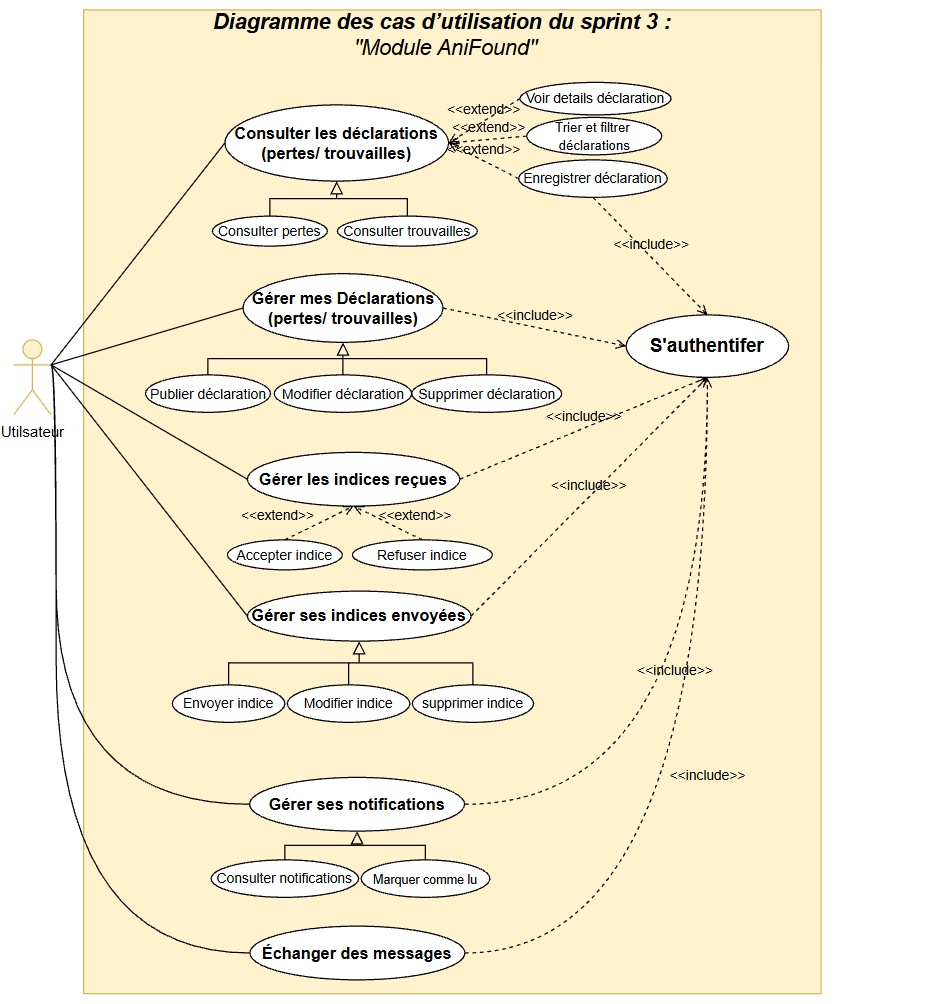
\includegraphics[width=0.92\linewidth, height=18.5cm, keepaspectratio]{images/usecase anifound.png}
    \caption{Diagramme des cas d’utilisation du sprint 3}
    \label{fig:usecase-sprint3}
\end{figure}
\newpage
\subsection{Descriptions textuelles des cas d’utilisation du sprint 3}  
Dans cette section, nous allons présenter les descriptions textuelles des cas d’utilisation du sprint 3
afin de détailler le comportement du système pour chaque fonctionnalité du module AniFound. 

\subsubsection{ Description textuelle du cas d’utilisation «Consulter déclarations de perte et de trouvaille » }    

La table \ref{tab:consulter_declarations} présente la description textuelle du cas d’utilisation « Consulter les déclarations de perte et de trouvaille » : 

\begin{longtable}{|c|p{11cm}|}
\caption{Description textuelle du cas d’utilisation "Consulter les déclarations de perte et de trouvaille"}
\label{tab:consulter_declarations} \\
\hline
\cellcolor{coloranifound} \textbf{Nom du cas d'utilisation } & Consulter les déclarations de perte et de trouvaille \\
\hline
\cellcolor{coloranifound} \textbf{Acteurs} & Utilisateur \\
\hline
\cellcolor{coloranifound} \textbf{Description } & Tout utilisateur peut consulter les annonces de perte et de trouvaille du module AniFound pour identifier un animal perdu ou retrouvé. \\
\hline
\cellcolor{coloranifound} \textbf{Pré-condition } & L’utilisateur doit avoir accès à la plateforme AniHub. \\
\hline
\cellcolor{coloranifound} \textbf{Post-condition } & L’utilisateur a consulté et éventuellement enregistré des déclarations pour un suivi ultérieur. \\
\hline
\cellcolor{coloranifound} \textbf{Scénario nominal } & 
\begin{enumerate}
\item L’utilisateur accède au module AniFound.
\item Le système redirige l’utilisateur vers le module AniFound.
\item L’utilisateur choisit la section « déclarations de perte » ou « déclarations de trouvaille ».
\item Le système affiche la liste des déclarations correspondantes.
\item L’utilisateur peut filtrer les déclarations selon différents critères (type, localisation, date).
\item L’utilisateur peut trier les déclarations par date (plus récentes ou plus anciennes).
\item Le système affiche les résultats filtrés et triés.
\item L’utilisateur peut sélectionner une déclaration pour consulter ses détails.
\item L’utilisateur peut enregistrer une déclaration dans sa liste d'enregistrements.
\item Le système ajoute la déclaration à la liste enregistrée de l’utilisateur.
\end{enumerate} \\
\hline
\end{longtable}
\newpage 
\subsubsection{Description textuelle du cas d’utilisation «Gérer déclarations de perte et de trouvaille»}
La table \ref{tab:gerer_declarations} présente la description textuelle du cas d’utilisation « Gérer les déclarations de perte et de trouvaille » :
\begin{longtable}{|c|p{11cm}|}
\caption{Description textuelle du cas d'utilisation "Gérer les déclarations de perte et de trouvaille"}
\label{tab:gerer_declarations} \\
\hline
\cellcolor{coloranifound}\textbf{Nom du cas d'utilisation } & Gérer les déclarations de perte et de trouvaille \\
\hline
\cellcolor{coloranifound}\textbf{Acteurs} & Utilisateur \\
\hline
\cellcolor{coloranifound}\textbf{Description } & L’utilisateur peut publier, modifier ou supprimer une déclaration de perte ou de trouvaille \\
\hline
\cellcolor{coloranifound}\textbf{Pré-condition } & L’utilisateur doit être authentifié \\
\hline
\cellcolor{coloranifound}\textbf{Post-condition } & La déclaration est ajoutée, modifiée ou supprimée avec succès. \\
\hline

\cellcolor{coloranifound}\textbf{Scénario nominal } &
\begin{enumerate}
\item L’utilisateur accède au module AniFound.
\item Le système redirige l’utilisateur vers "AniFound".

\item \textbf{Cas publication :}
\begin{itemize}
\item L’utilisateur choisit « perte » ou « trouvaille ».
\item L’utilisateur clique sur « Publier une déclaration ».
\item Le système affiche le formulaire d’ajout.
\item L’utilisateur remplit les informations et valide.
\item Le système vérifie et enregistre la déclaration.
\end{itemize}

\item L’utilisateur accède à « Mon espace AniFound ».
\item Le système affiche ses déclarations.

\item \textbf{Cas modification :}
\begin{itemize}
\item L’utilisateur sélectionne une déclaration.
\item L’utilisateur clique sur « Modifier ».
\item Le système affiche le formulaire pré-rempli.
\item L’utilisateur modifie et valide.
\item Le système enregistre les modifications.
\end{itemize}

\item \textbf{Cas suppression :}
\begin{itemize}
\item L’utilisateur sélectionne une déclaration.
\item L’utilisateur clique sur « Supprimer ».
\item Le système demande une confirmation.
\item L’utilisateur confirme.
\item Le système supprime la déclaration.
\end{itemize}

\item Le système affiche un message de succès.
\end{enumerate} \\

\hline
\cellcolor{coloranifound}\textbf{Scénario alternatif :} &
\begin{itemize}
\item Erreur de publication : message d’erreur affiché.
\item Erreur de modification : message d’erreur affiché.
\item Annulation suppression : Déclaration conservée.
\end{itemize} \\
\hline

\end{longtable}
\newpage 
\subsubsection{ Description textuelle des cas d’utilisation «Gérer les indices reçus et envoyés» }   
La table \ref{tab:gerer_indices_anifound} présente la description textuelle du cas d’utilisation «Gérer les indices reçus et envoyés» :
\begin{longtable}{|c|p{11cm}|} 
\caption{Description textuelle des cas d'utilisation "Gérer les indices reçus et envoyés"}
\label{tab:gerer_indices_anifound} \\
\hline
\cellcolor{coloranifound}\textbf{Nom du cas d'utilisation } & Gérer les indices reçus et envoyés \\
\hline
\cellcolor{coloranifound}\textbf{Acteurs} & Utilisateur \\
\hline
\cellcolor{coloranifound}\textbf{Description } & L’utilisateur consulte et gère les indices de ses déclarations de trouvaille pour prouver la propriété d’un animal. \\
\hline
\cellcolor{coloranifound}\textbf{Pré-condition } & L’utilisateur est authentifié et dispose de déclarations de trouvaille ou a déjà envoyé des indices. \\
\hline
\cellcolor{coloranifound}\textbf{Post-condition } & Les indices sont consultés et leur statut est mis à jour (en attente, validé ou rejeté). \\
\hline

\cellcolor{coloranifound}\textbf{Scénario nominal } &
\begin{enumerate}
\item L’utilisateur accède au module AniFound.
\item Il sélectionne « Mon espace AniFound ».
\item Le système affiche les déclarations de l’utilisateur.
\item L’utilisateur choisit une déclaration spécifique.
\item Le système affiche les indices liés à cette déclaration.
\item Selon le type d’interaction :

\begin{itemize}
\item \textbf{Cas 1 : Indices reçus}
\begin{enumerate}
\item L’utilisateur consulte la liste des indices reçus.
\item Il ouvre un indice reçu .
\item Il valide ou rejette l’indice .
\item Le système met à jour le statut de l’indice.
\item Le système affiche un message de confirmation.
\end{enumerate}

\item \textbf{Cas 2 : Indices envoyés}
\begin{enumerate}
\item L’utilisateur consulte la liste des indices qu’il a envoyés.
\item Il sélectionne un indice pour en voir les détails.
\item Il consulte son statut (en attente, validé ou rejeté).
\item Le système affiche les mises à jour du statut.
\end{enumerate}
\end{itemize}

\end{enumerate} \\
\hline

\cellcolor{coloranifound}\textbf{Scénario alternatif :} &
\begin{itemize}
\item Erreur lors du chargement ou du traitement : le système affiche un message d’erreur sans modifier les données.
\end{itemize} \\
\hline

\end{longtable}

\newpage

\subsection{Diagramme de classes du sprint 3} 
Dans cette section, nous présentons le diagramme de classes du sprint 3, qui regroupe l’ensemble des classes constituant le système. 


La figure \ref{fig:class_diagram_anifound} illustre le diagramme de classes pour ce sprint :



\begin{figure}[H]
    \centering
    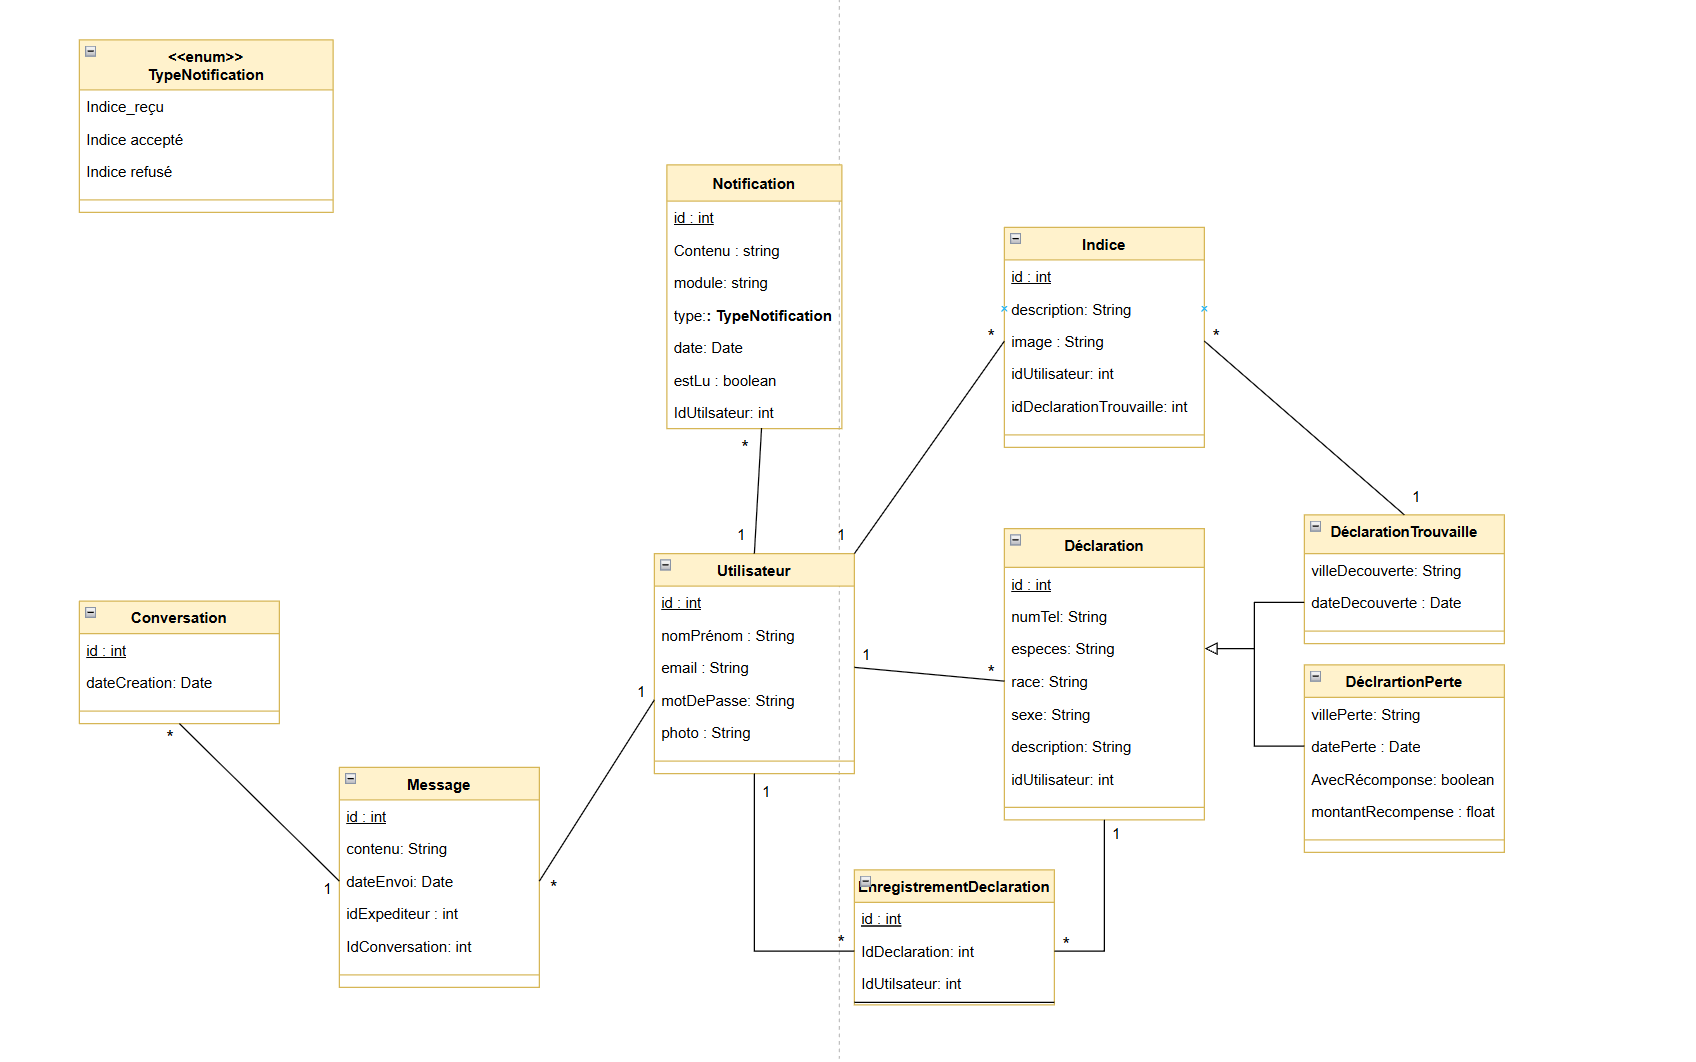
\includegraphics[width=1.15\textwidth,height=16cm]{images/diagramme classe anifoundd.png}
    \caption{Diagramme de classes du sprint 3}
    \label{fig:class_diagram_anifound}
\end{figure}

\subsection{Diagrammes de séquences du sprint 3}

Dans cette section, nous présentons les diagrammes de séquence du sprint 3, illustrant les principales interactions entre les différents composants du système et les flux de communication associés aux nouvelles fonctionnalités implémentées . 
\newpage
\subsubsection{Diagramme de séquence : gérer mes déclarations de perte ou de trouvaille}

La figure \ref{fig:gerer_declarations_sq} illustre les interactions entre l’utilisateur et le système pour la gestion des déclarations de perte ou de trouvaille.

\begin{figure}[H]
    \centering
    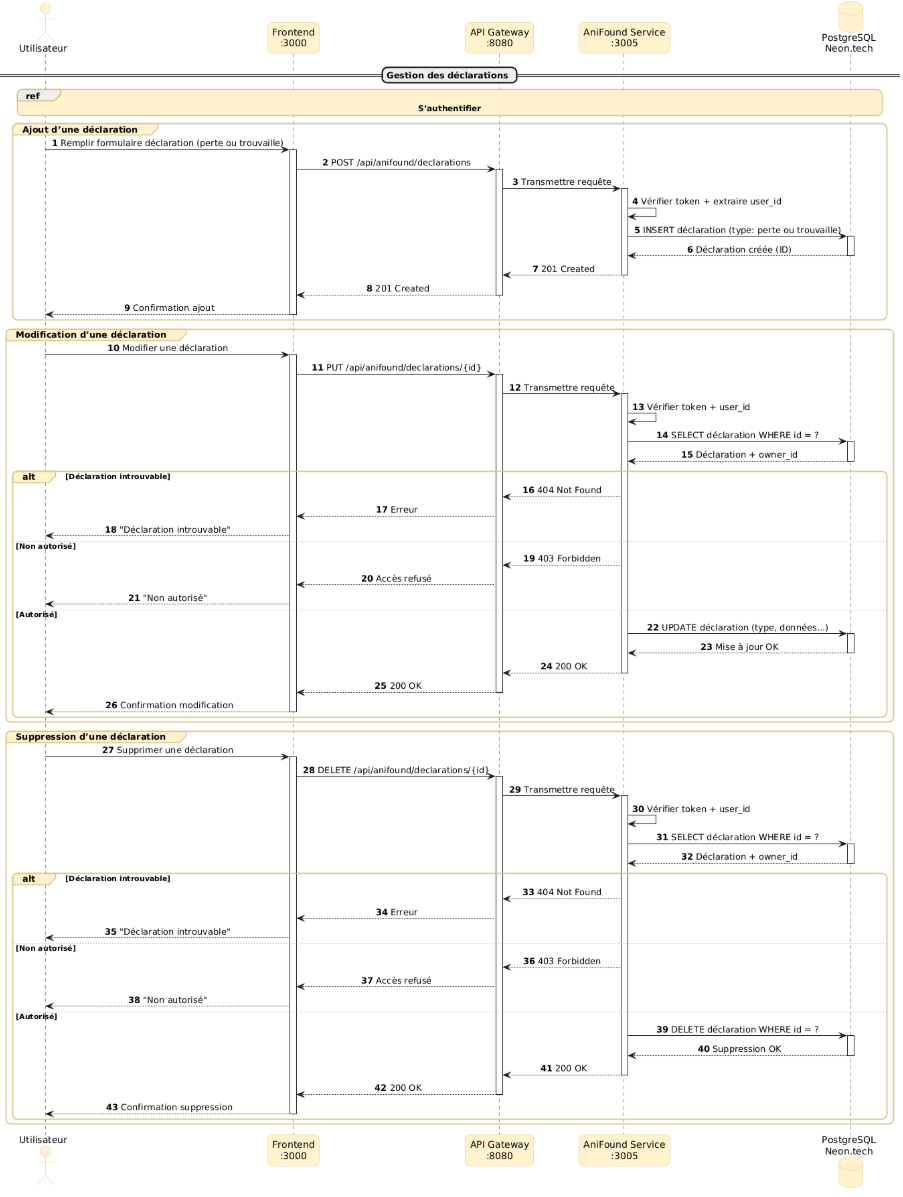
\includegraphics[width=0.7\textwidth]{images/gerer declarations sq.png}
    \caption{Diagramme de séquence : gérer mes déclarations de perte ou de trouvaille}
    \label{fig:gerer_declarations_sq}
\end{figure}
\newpage  
\subsubsection{Diagramme de séquence : gérer mes indices reçus}

La figure \ref{fig:gerer_indices_recus_sq} illustre les différentes interactions entre l’utilisateur et le système lors de la gestion des indices reçus liés aux déclarations de perte ou de trouvaille. Elle montre le processus de consultation des indices, ainsi que les actions possibles de validation ou d’ignorance d’un indice. Les échanges entre le Frontend, l’API Gateway, le microservice AniFound, la base de données et le service de notification sont également présentés afin de mettre en évidence le traitement complet d’un indice reçu : 
\begin{figure}[H]
    \centering
    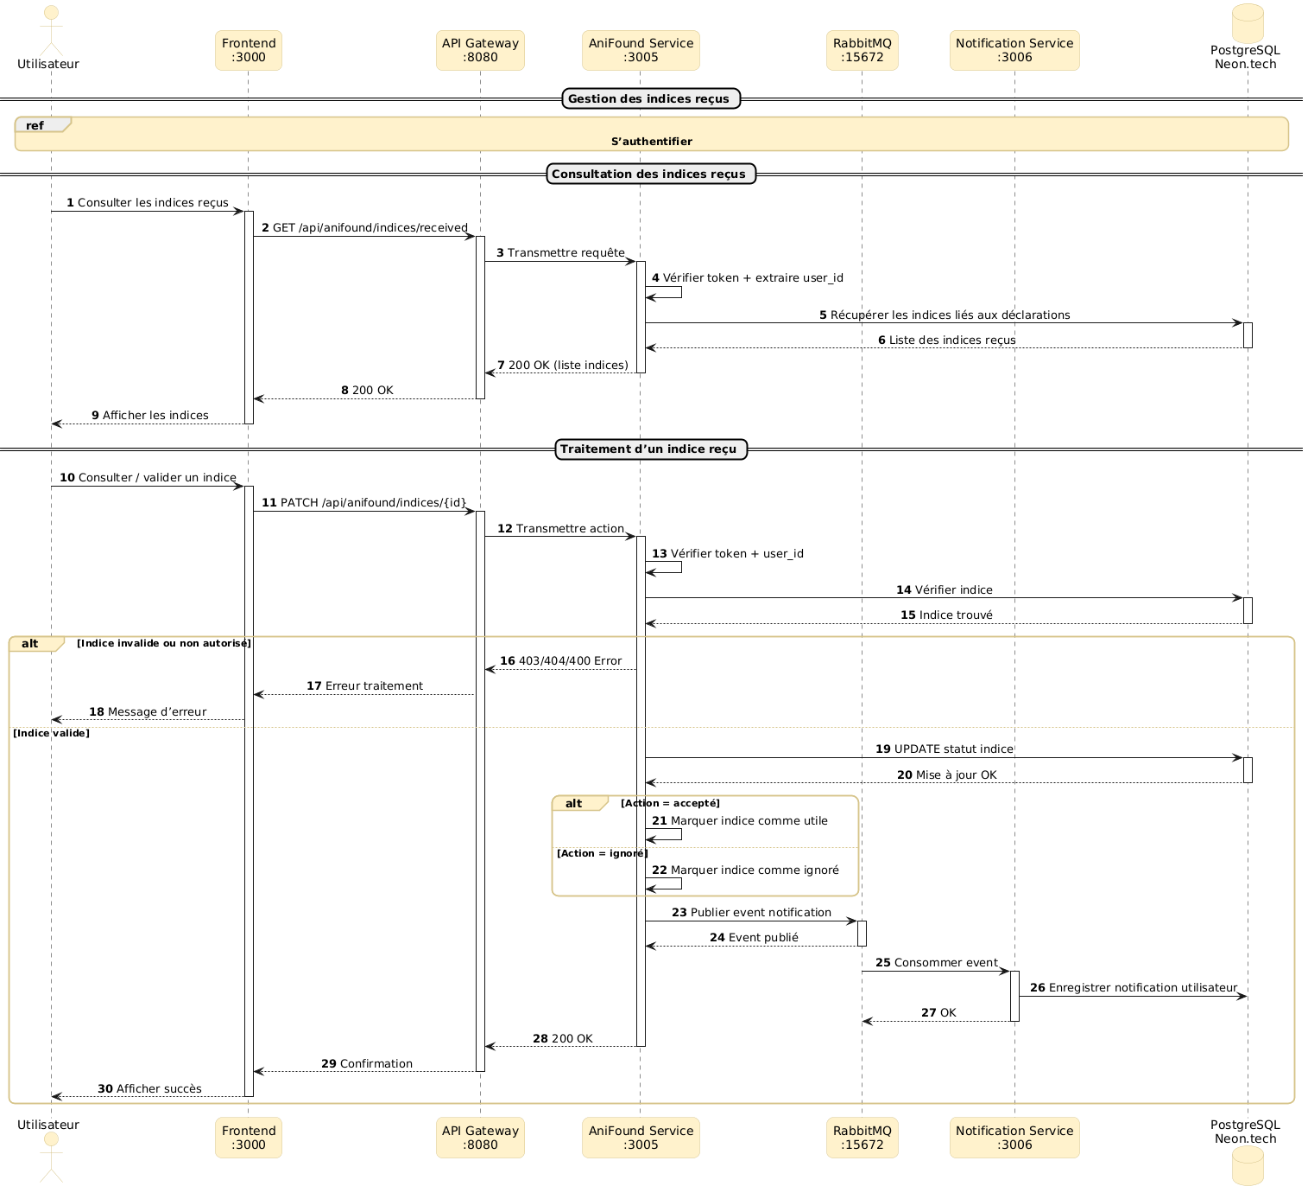
\includegraphics[width=1\textwidth]{images/gerer indice recu sq.png}
    \caption{Diagramme de séquence : gérer mes indices reçus}
\end{figure}
\newpage
\subsection{Réalisation du sprint 3 }

Dans cette partie, nous présentons les différentes interfaces graphiques de l’application développée, en lien avec ce sprint :

\subsubsection{Menu principal de l’application AniHub et interface d’accueil AniFound} 

La figure \ref{fig:menu_anifound_accueil} illustre le menu principal de l’application AniHub ainsi que l’interface d’accueil du module AniFound.

\begin{figure}[h!]
    \centering
    
    \begin{minipage}{0.48\textwidth}
        \centering
        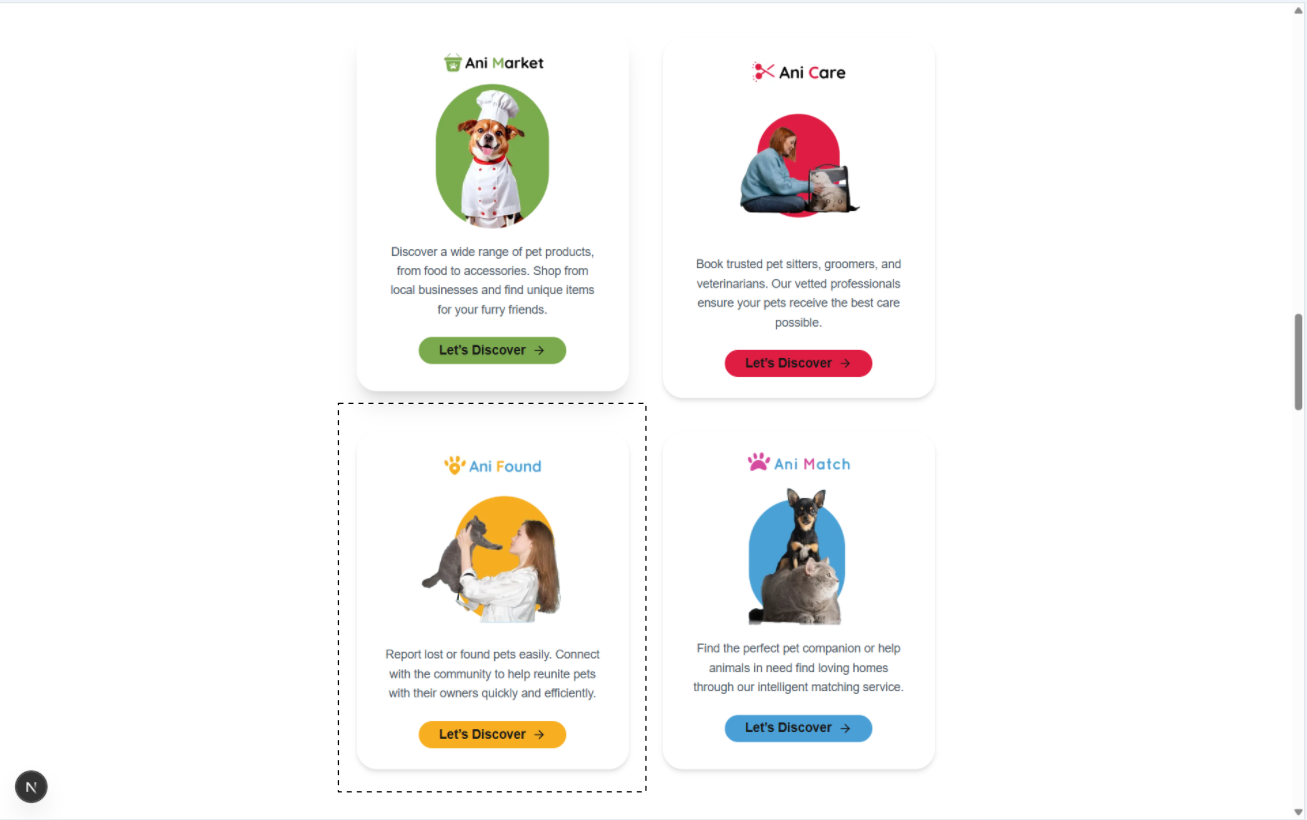
\includegraphics[width=0.85\textwidth]{images/menu anifound.png}
        \caption{Menu principal de l’application AniHub}
        \label{fig:menu_anihub_anifound}
    \end{minipage}
    \hfill
    \begin{minipage}{0.48\textwidth}
        \centering
        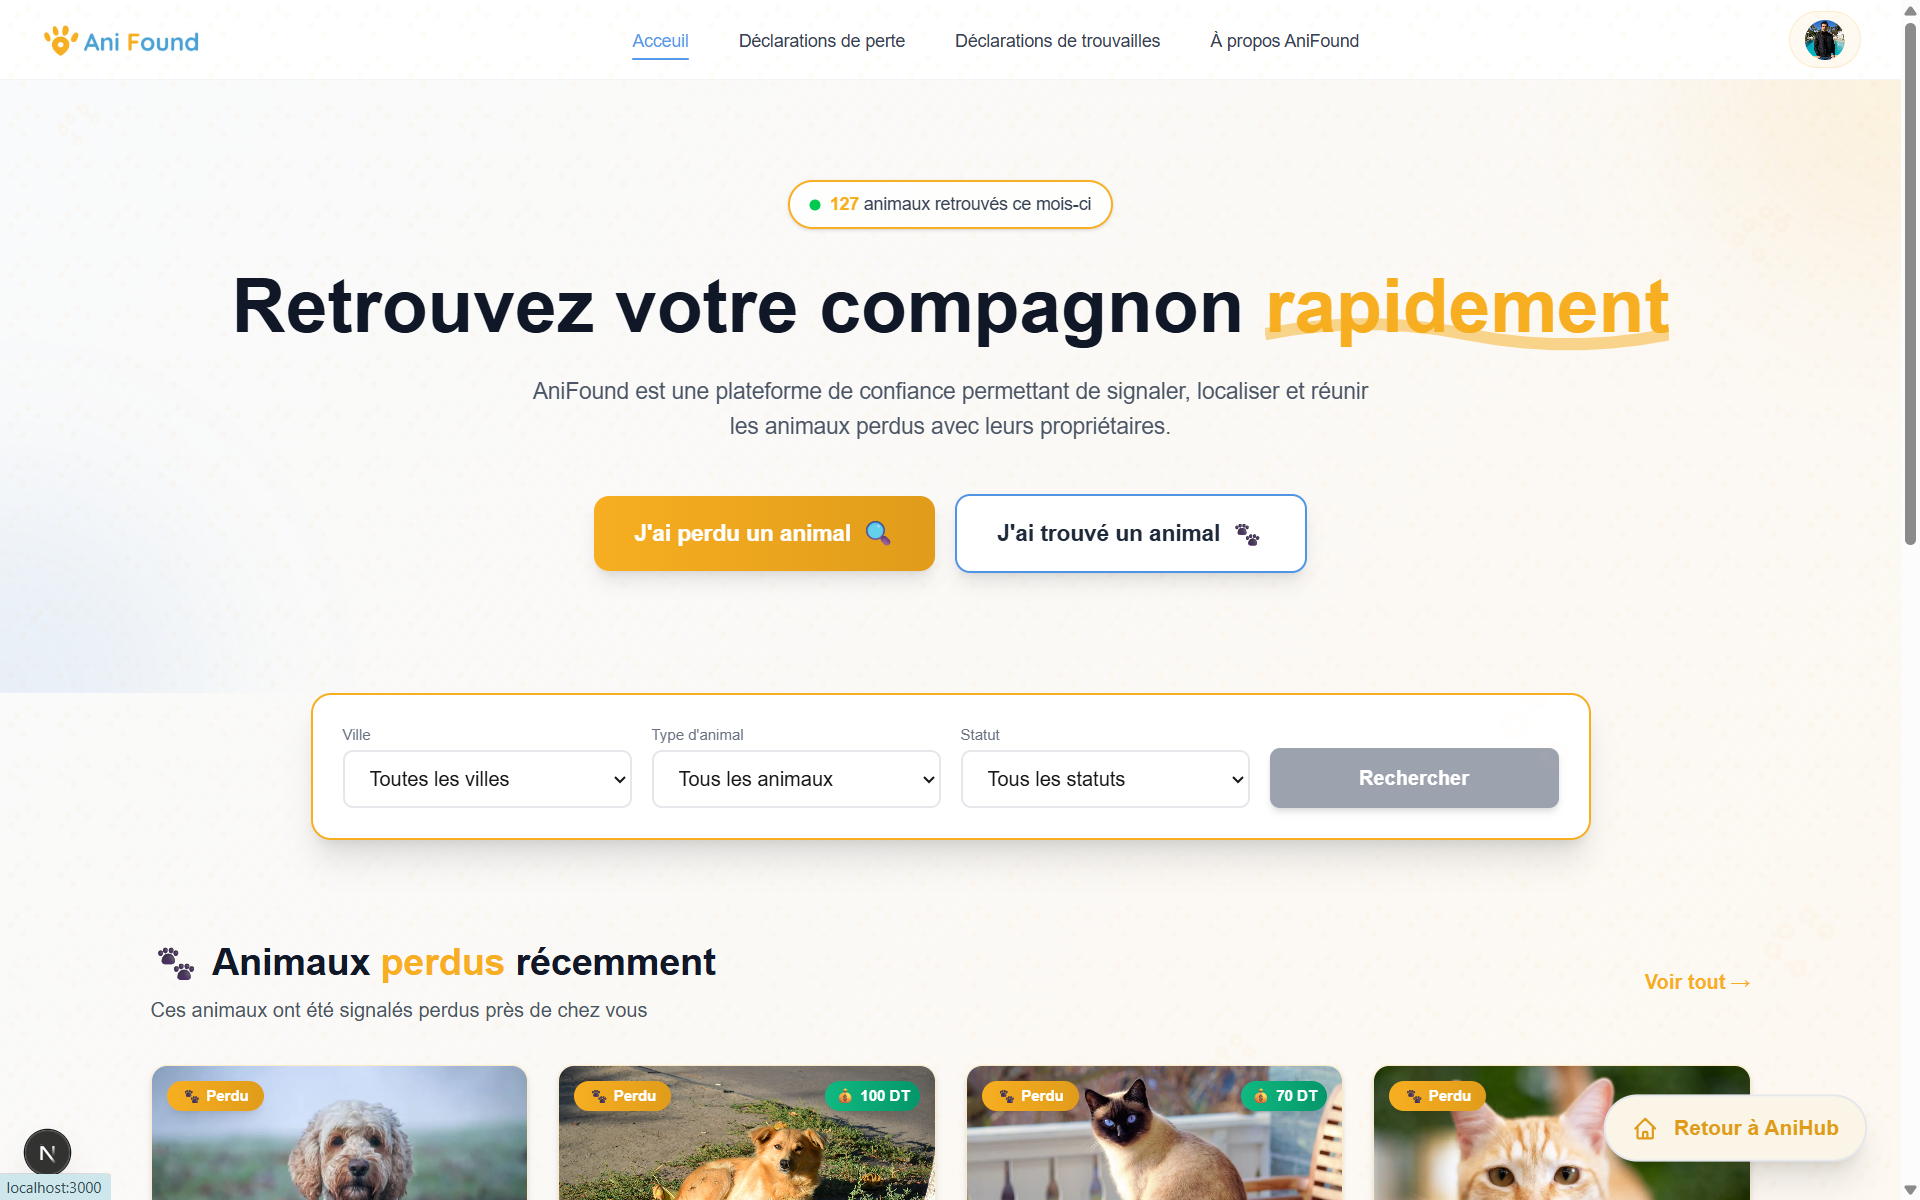
\includegraphics[width=0.85\textwidth]{images/acceuil anifound.png}
        \caption{Interface d’accueil AniFound}
        \label{fig:acceuil_anifound}
    \end{minipage}

\end{figure}  

\subsubsection{Interfaces d’annonce de perte et de trouvaille}

La figure \ref{fig:annonces_perte_trouvaille} illustre les interfaces de création d’une annonce de perte et de trouvaille.

\begin{figure}[h!]
    \centering
    
    \begin{minipage}{0.48\textwidth}
        \centering
        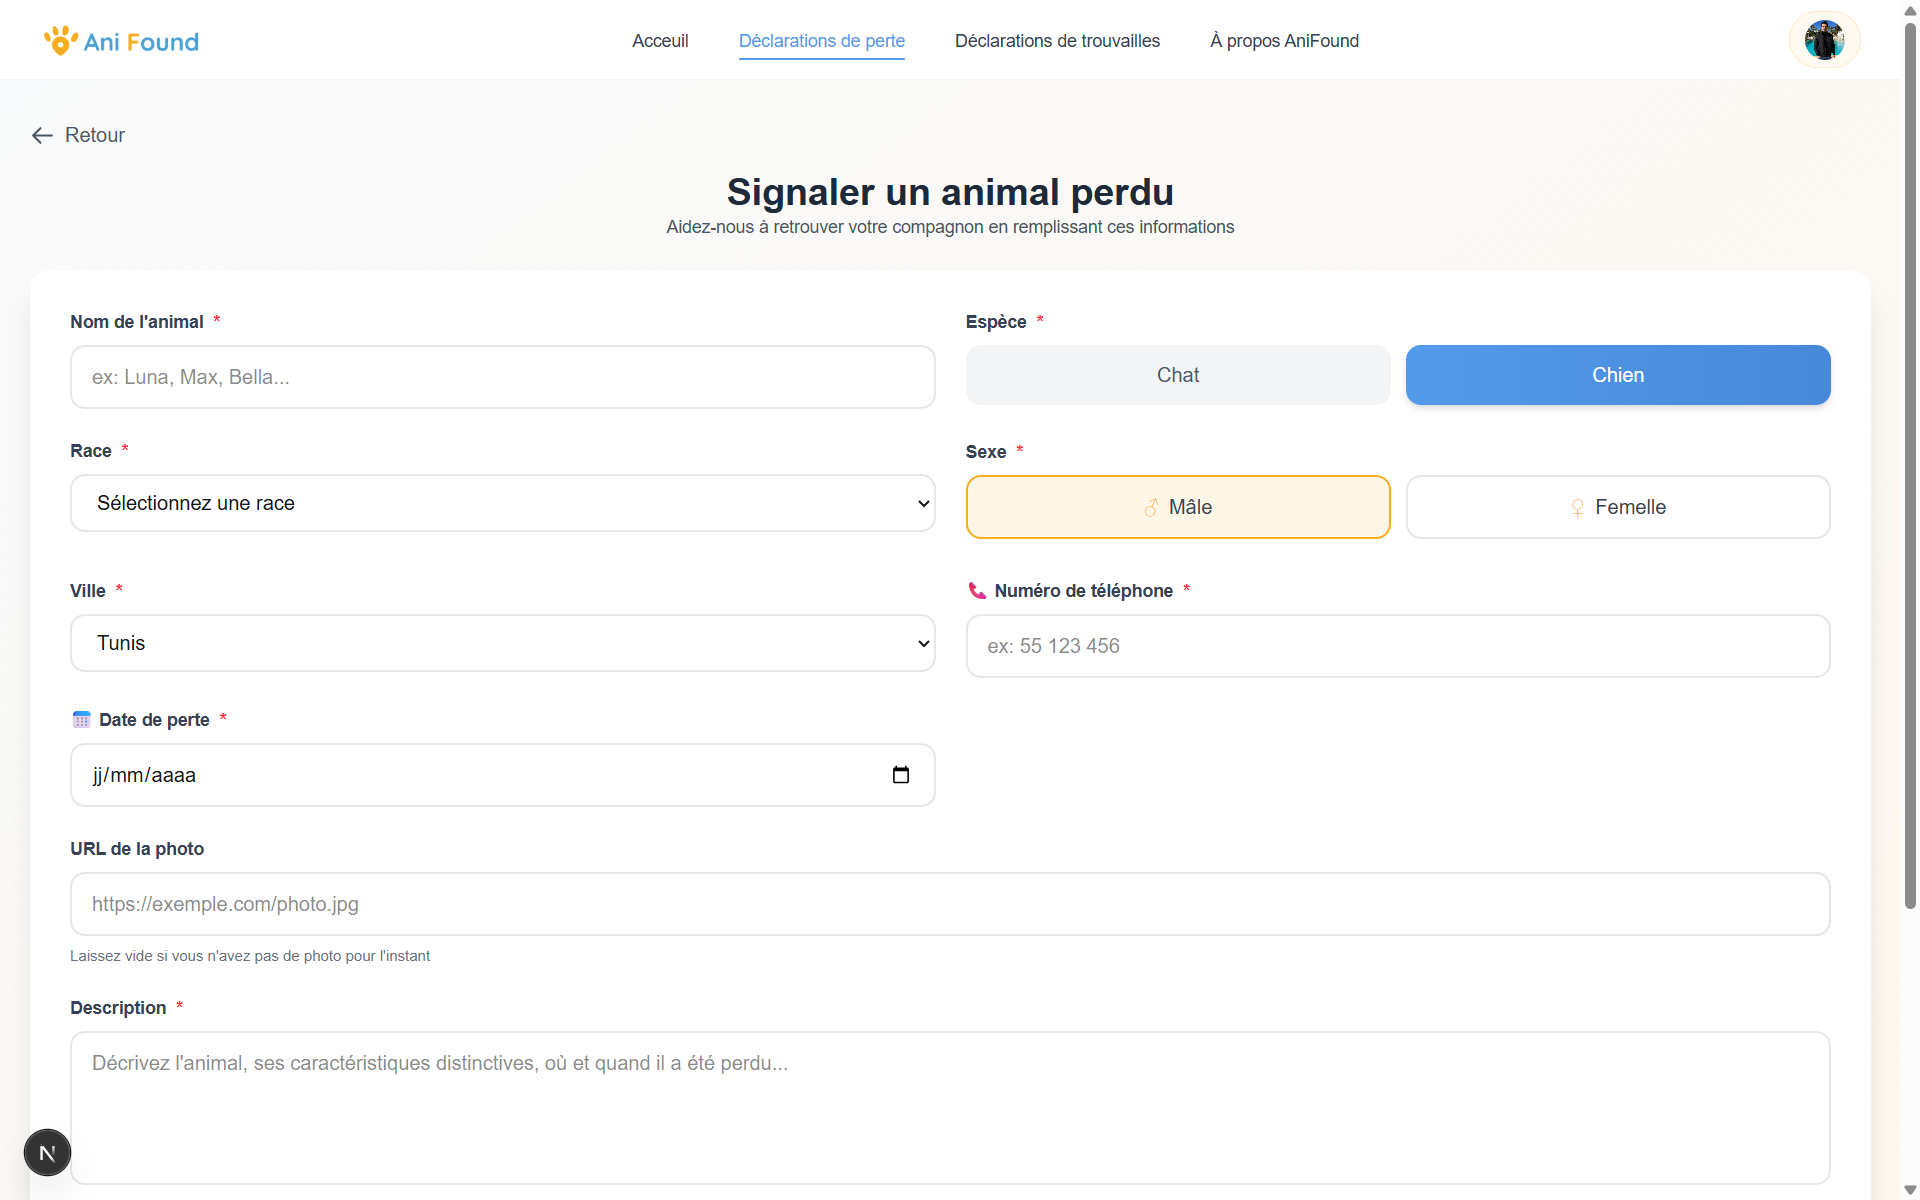
\includegraphics[width=0.77\textwidth]{images/declarer perte .png}
        \caption{Interface d’annonce de perte d’un animal}
        \label{fig:annonce_perte}
    \end{minipage}
    \hfill
    \begin{minipage}{0.48\textwidth}
        \centering
        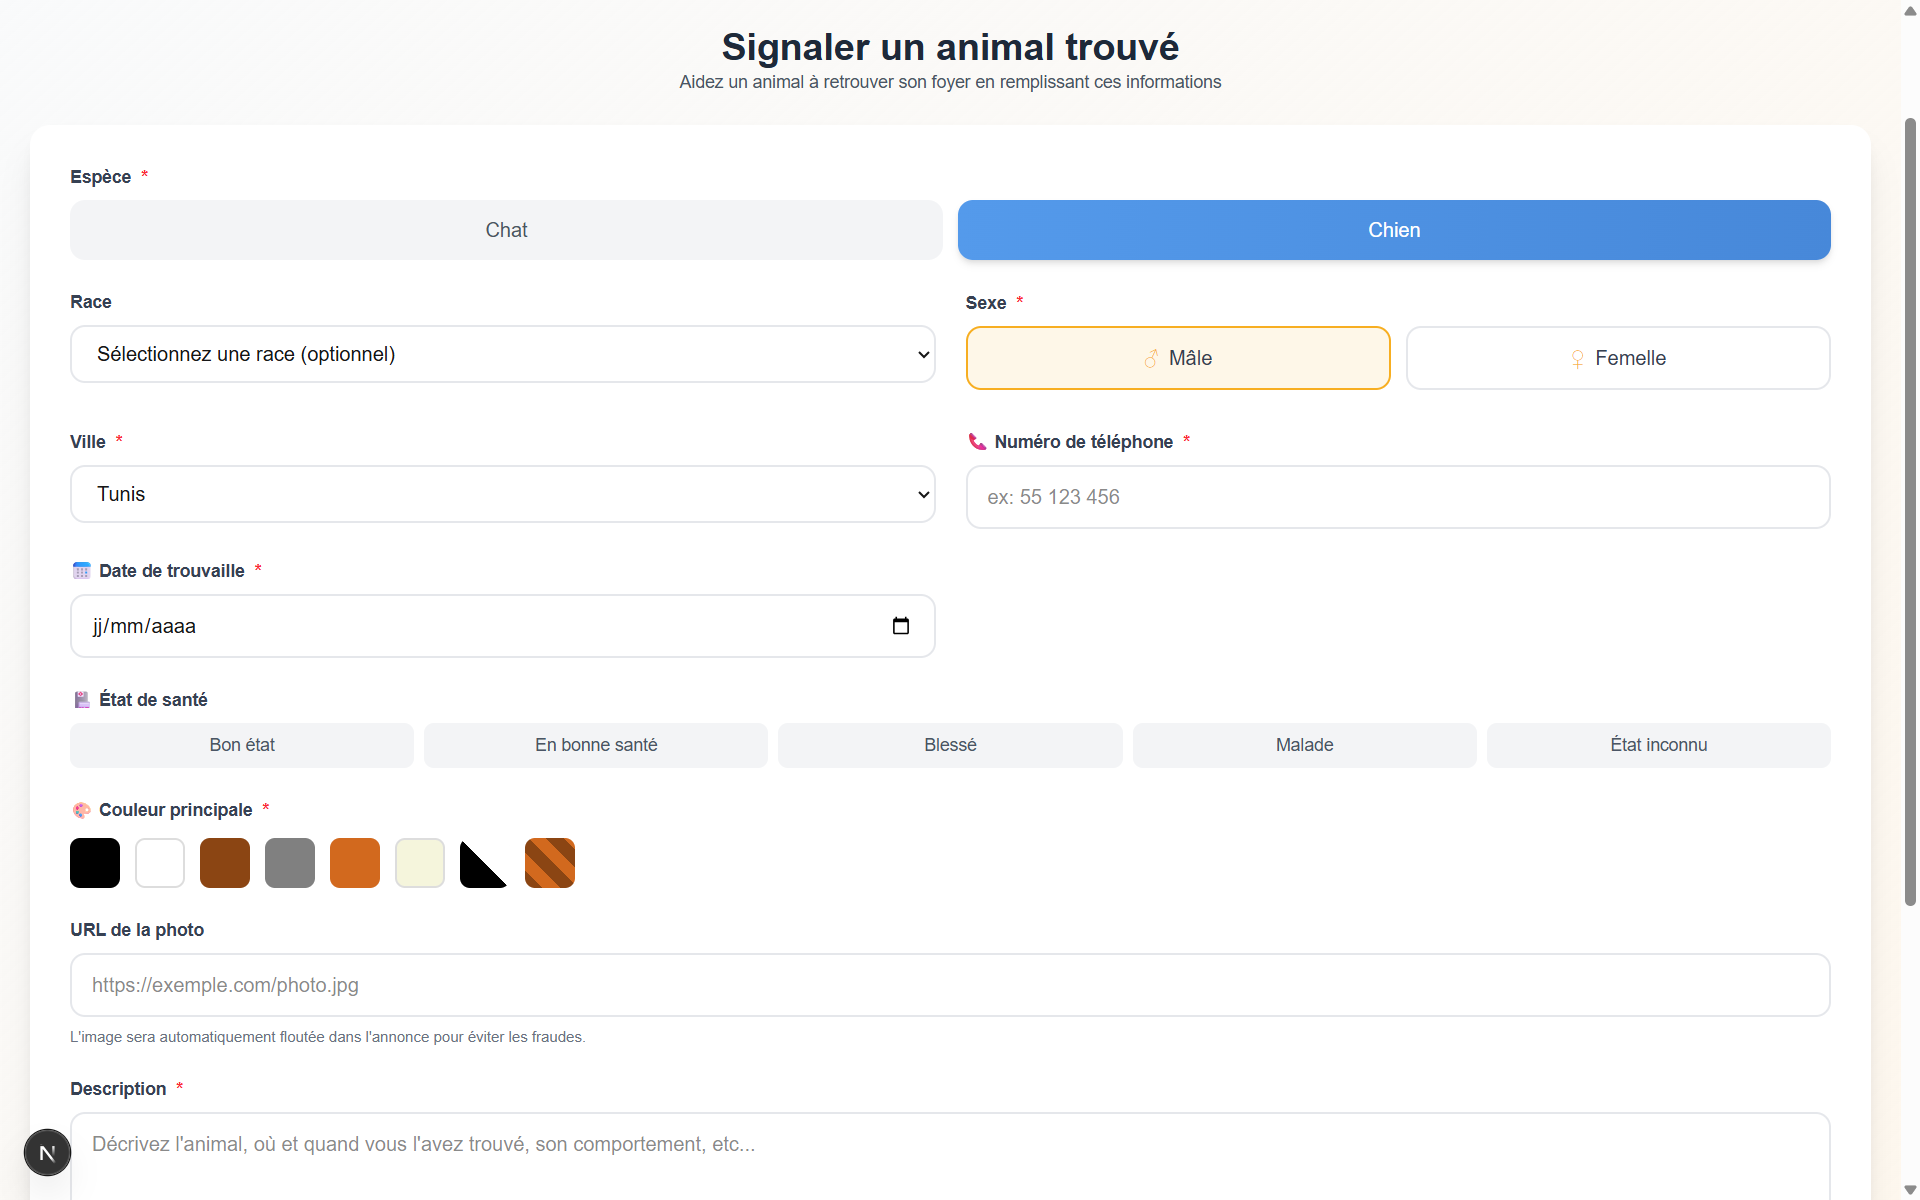
\includegraphics[width=0.77\textwidth]{images/decalarer trouvaille.png}
        \caption{Interface d’annonce de trouvaille d’un animal}
        \label{fig:annonce_trouvaille}
    \end{minipage}

\end{figure}

\newpage

\subsubsection{Interface des déclarations de trouvaille}

La figure \ref{fig:liste_trouvailles} illustre la liste des déclarations de trouvaille disponibles dans le système.

\begin{figure}[h!]
    \centering
    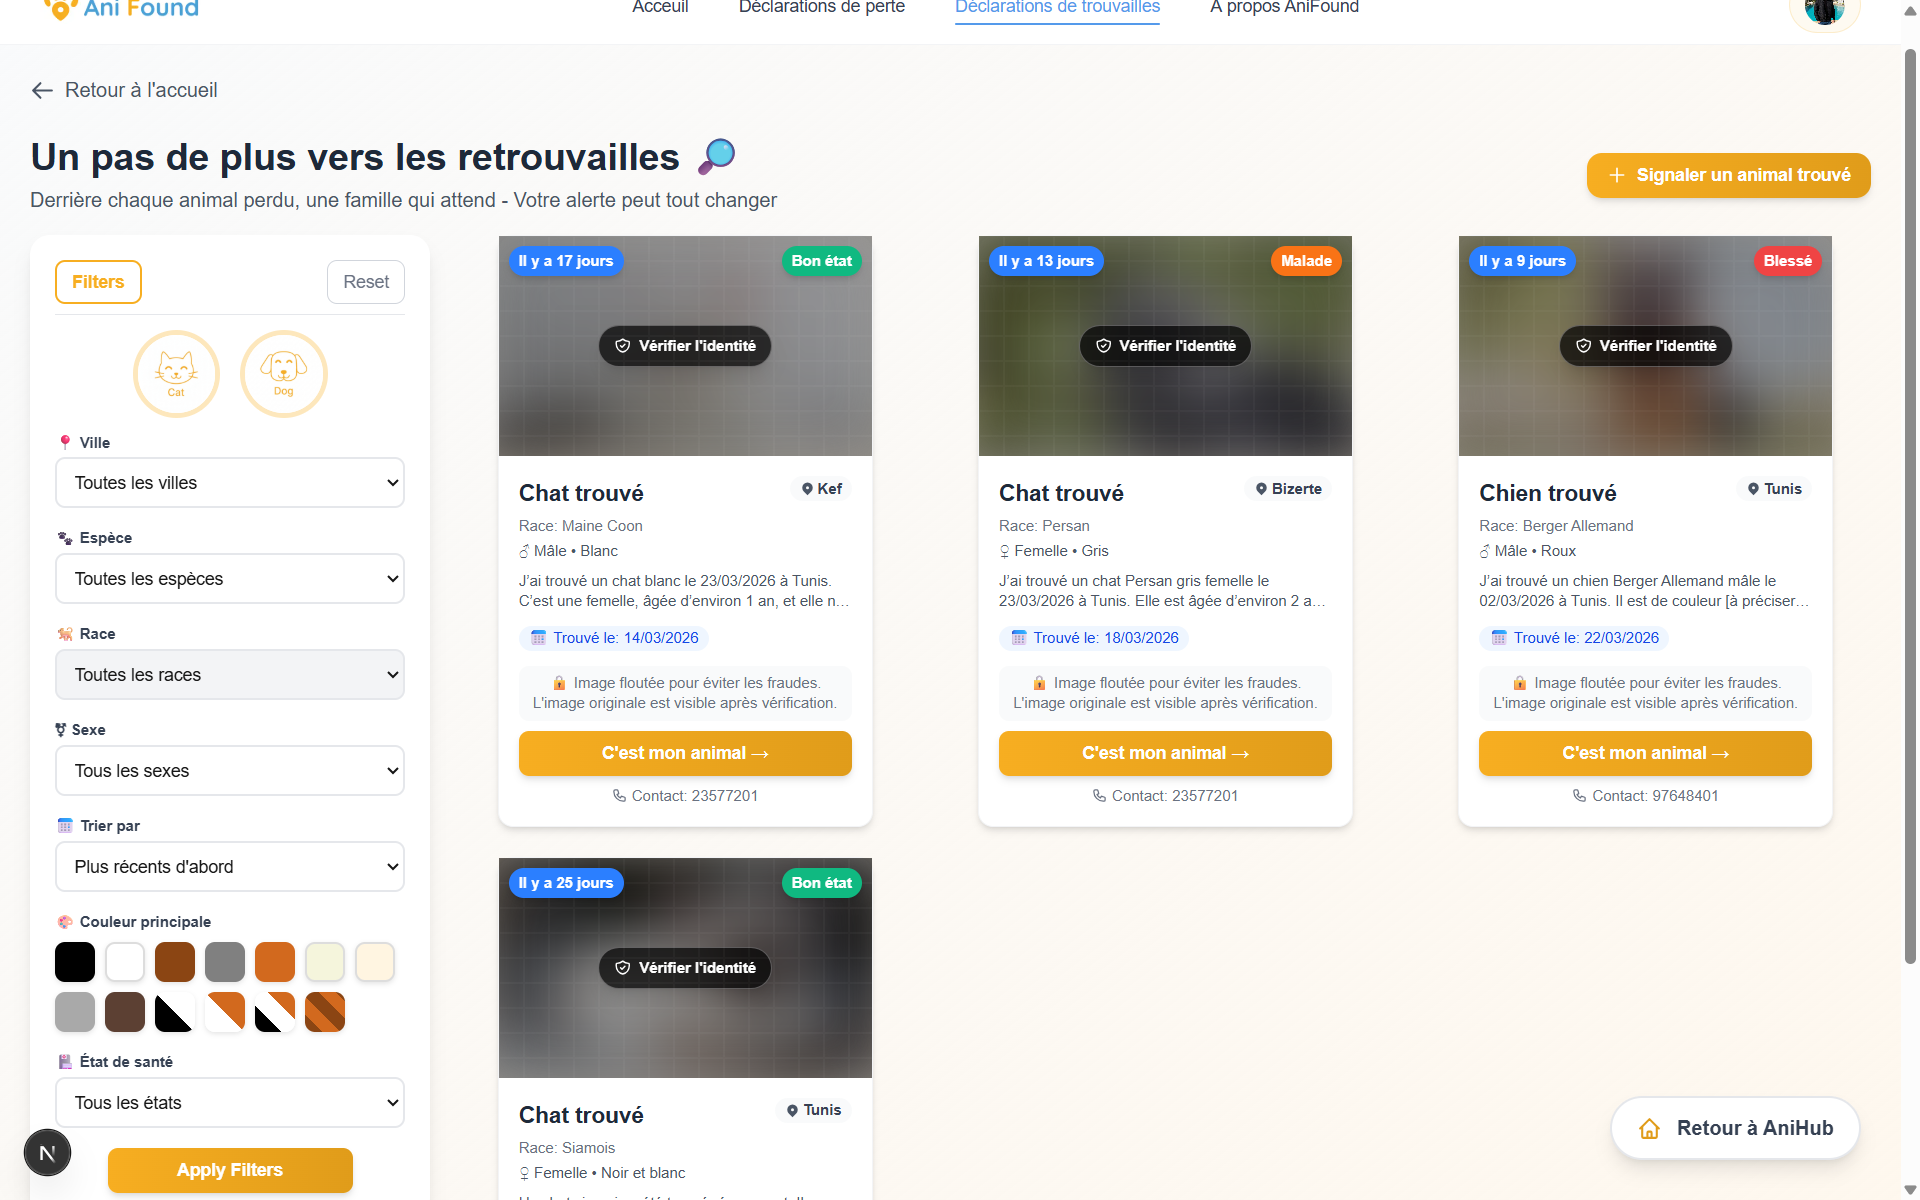
\includegraphics[width=0.77\textwidth]{images/page trouvailles.png}
    \caption{Interface des déclarations de trouvaille}
    \label{fig:liste_trouvailles}
\end{figure}  

\subsubsection{Interface de détails d’une déclaration de trouvaille}

La figure \ref{fig:details_trouvaille} illustre les détails complets d’une déclaration de trouvaille.

\begin{figure}[h!]
    \centering
    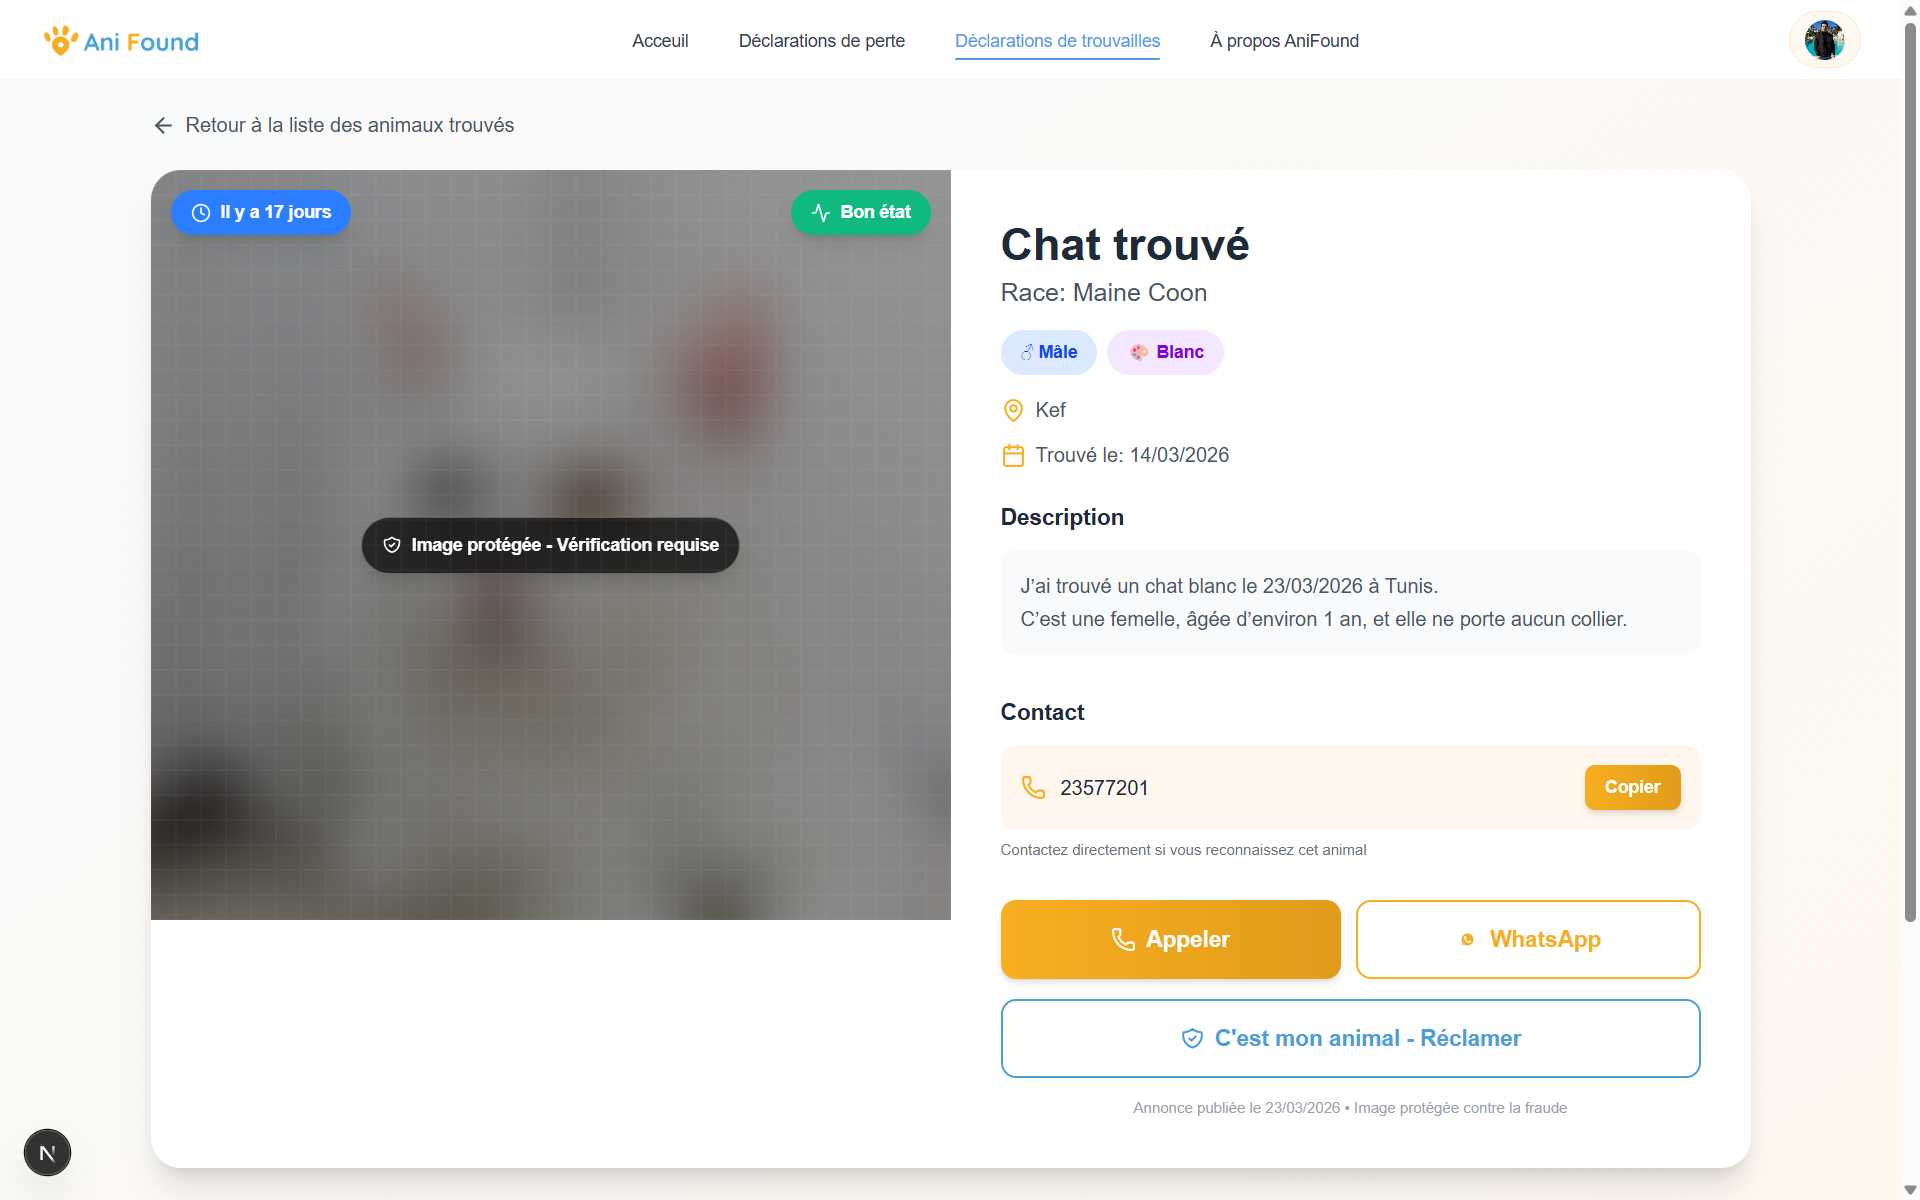
\includegraphics[width=0.77\textwidth]{images/details trouvaille.png}
    \caption{Interface de détails d’une déclaration de trouvaille}
    \label{fig:details_trouvaille}
\end{figure} 

\subsubsection{Interface d’envoi d’un indice pour une déclaration de trouvaille}

La figure \ref{fig:envoi_indice} illustre le formulaire d’envoi d’un indice pour une déclaration de trouvaille.

\begin{figure}[h!]
    \centering
    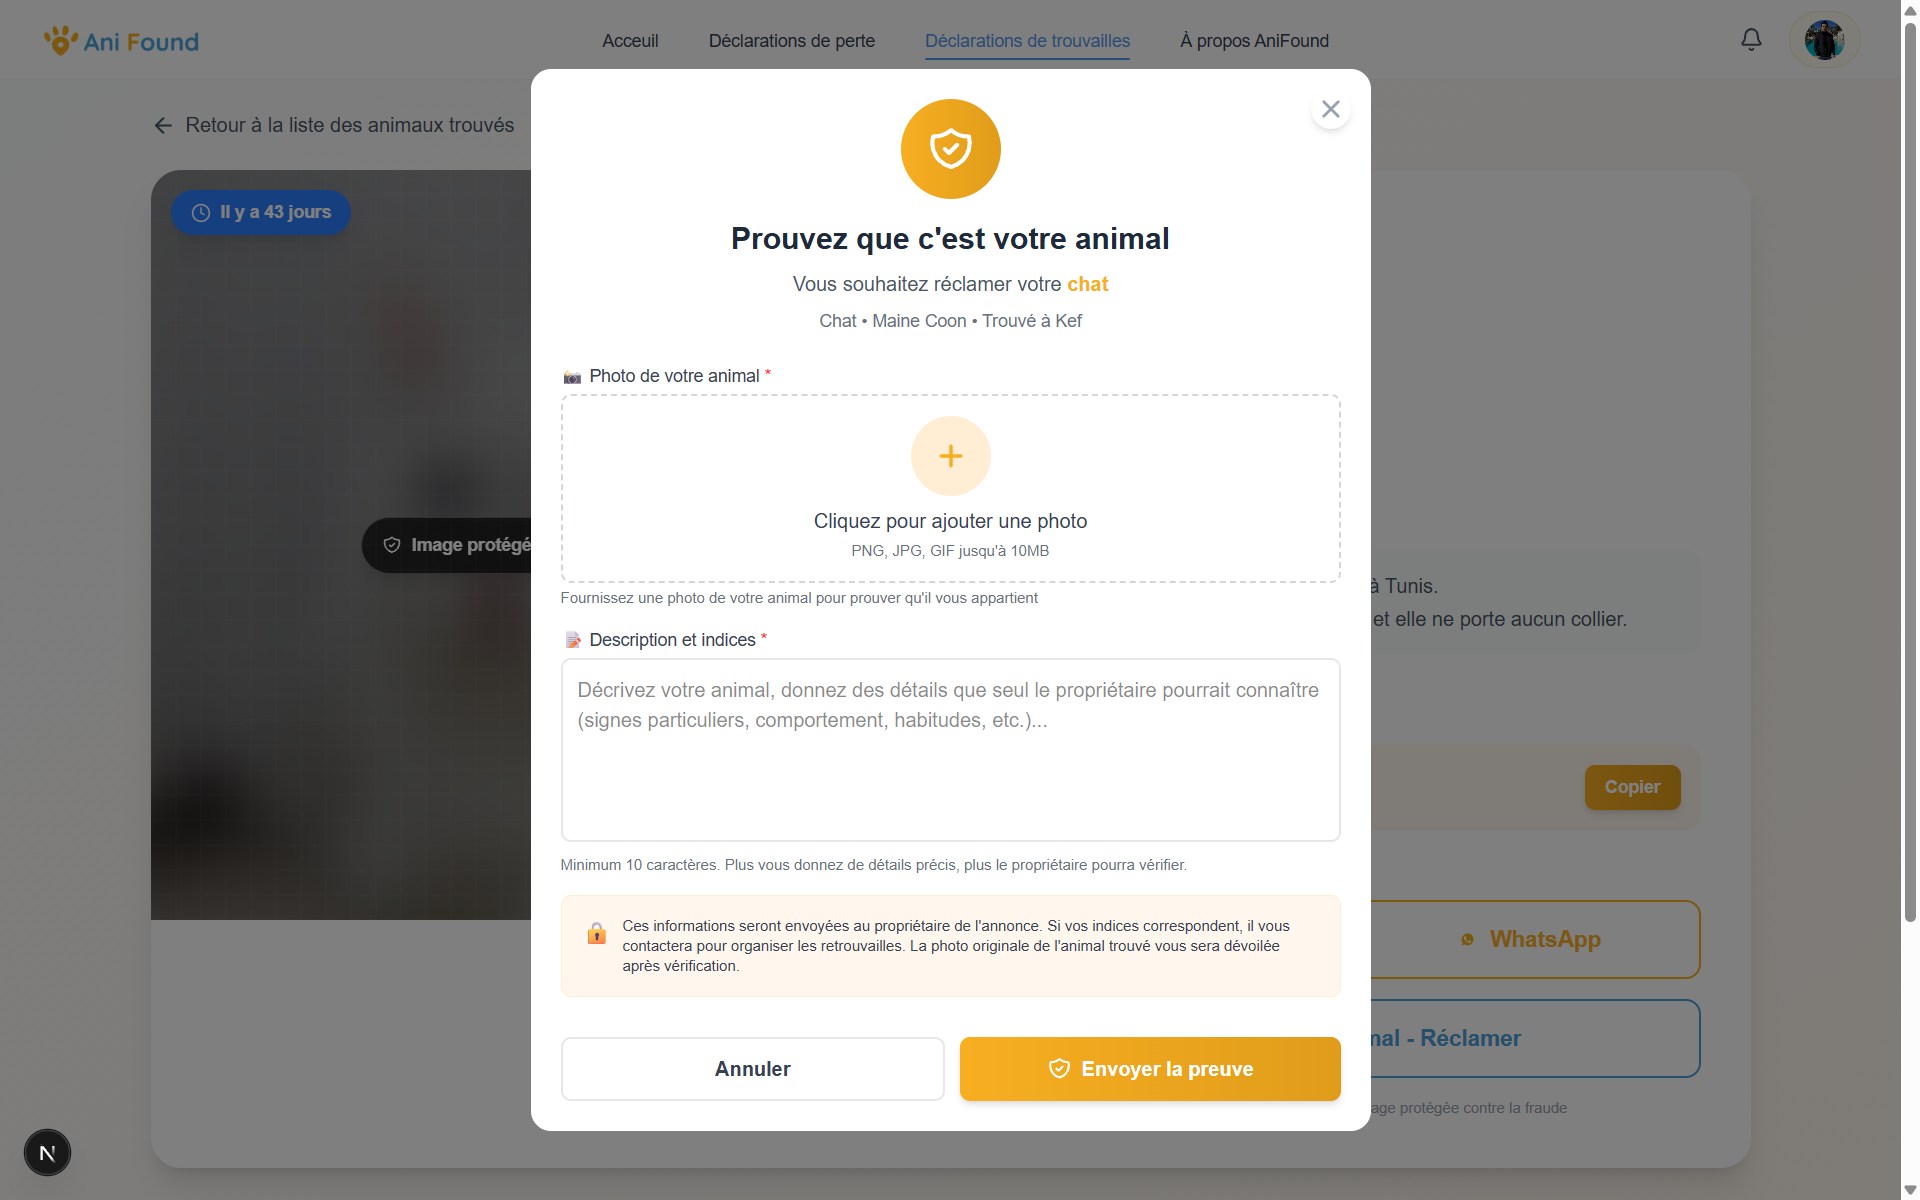
\includegraphics[width=0.77\textwidth]{images/envoyer indice.png}
    \caption{Interface d’envoi d’un indice pour une déclaration de trouvaille}
    \label{fig:envoi_indice}
\end{figure}

\subsubsection{Interface des déclarations de perte}

La figure \ref{fig:liste_pertes} illustre la liste des déclarations de perte des animaux.

\begin{figure}[h!]
    \centering
    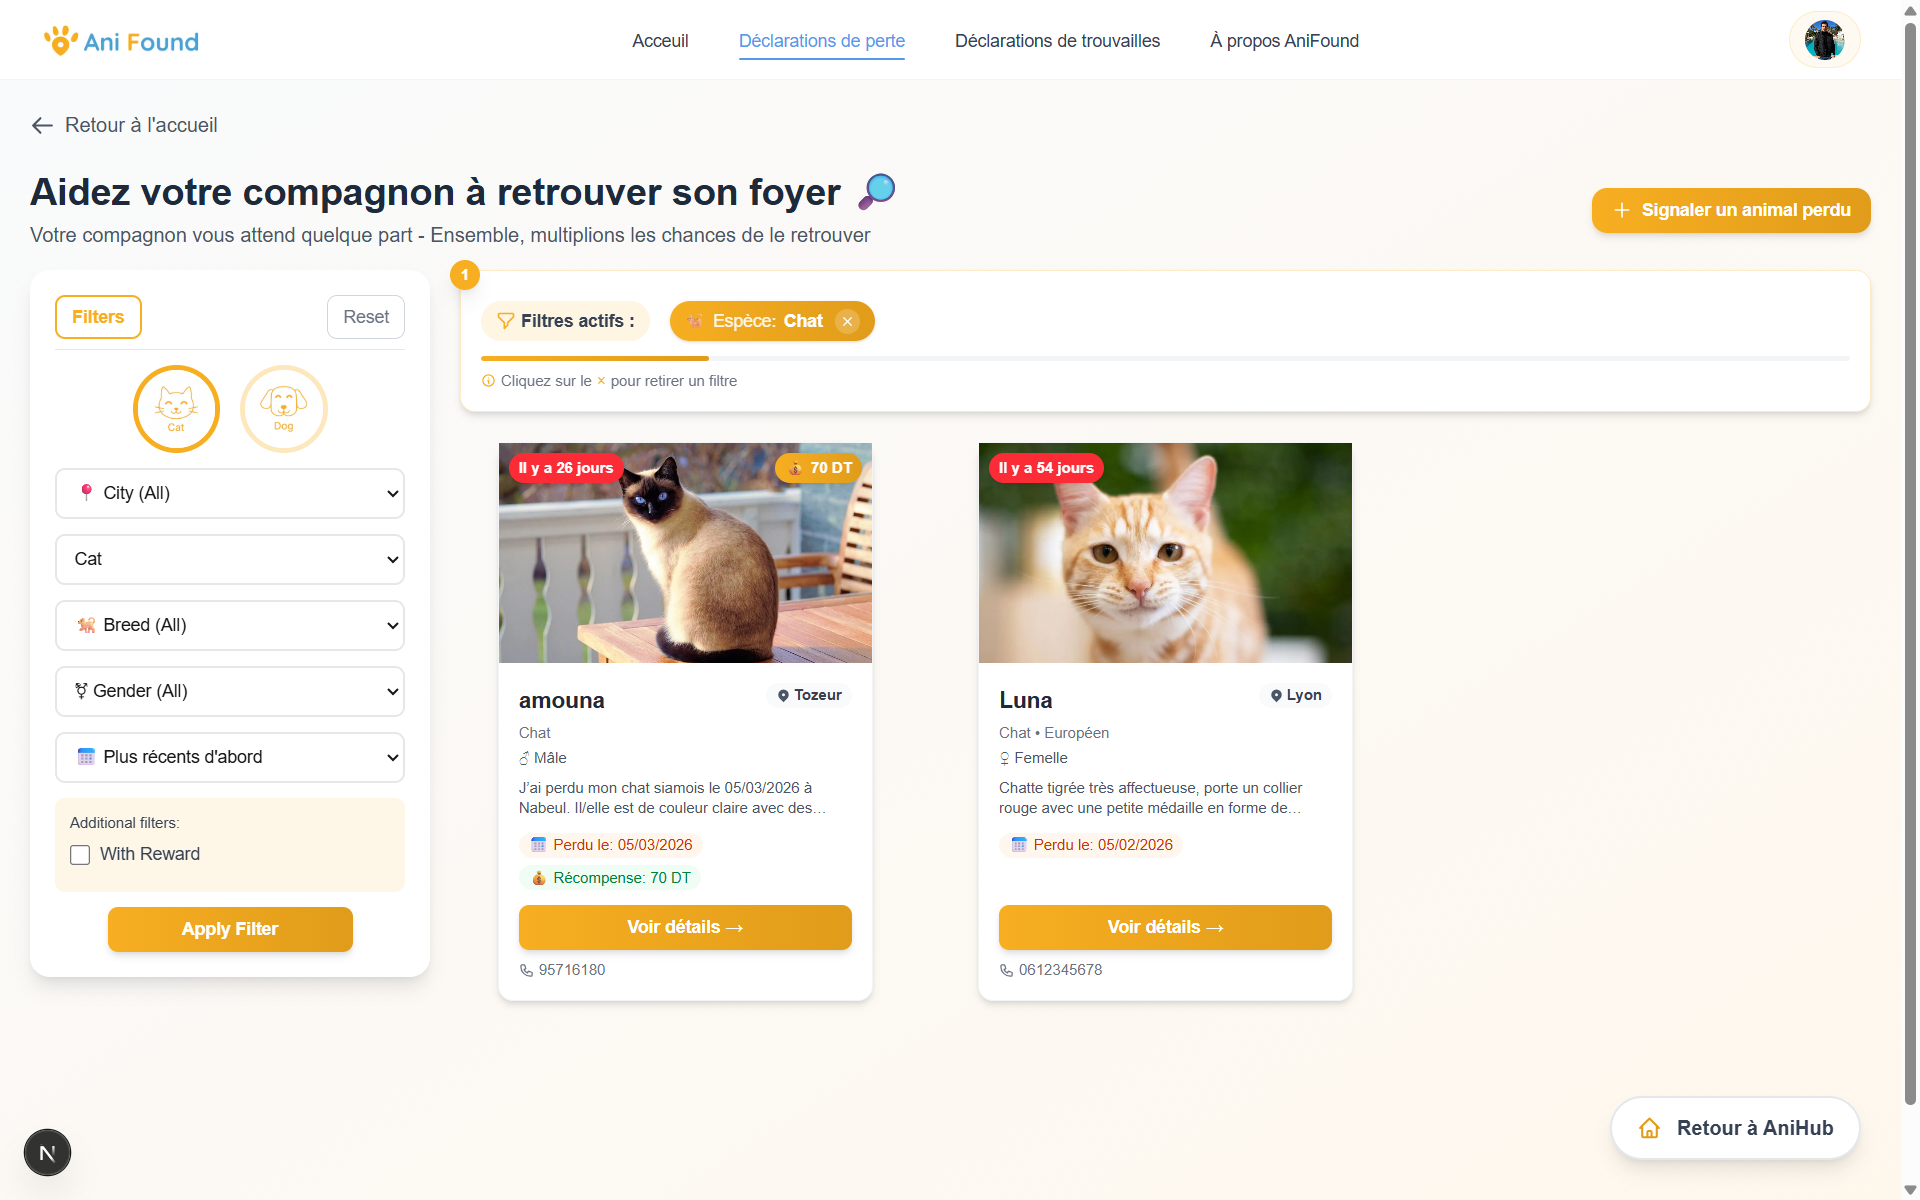
\includegraphics[width=0.77\textwidth]{images/page perte.png}
    \caption{Interface des déclarations de perte}
    \label{fig:liste_pertes}
\end{figure} 

\newpage

\subsubsection{Interface de détails d’une déclaration de perte}

La figure \ref{fig:details_perte} illustre les détails d’une déclaration de perte.

\begin{figure}[h!]
    \centering
    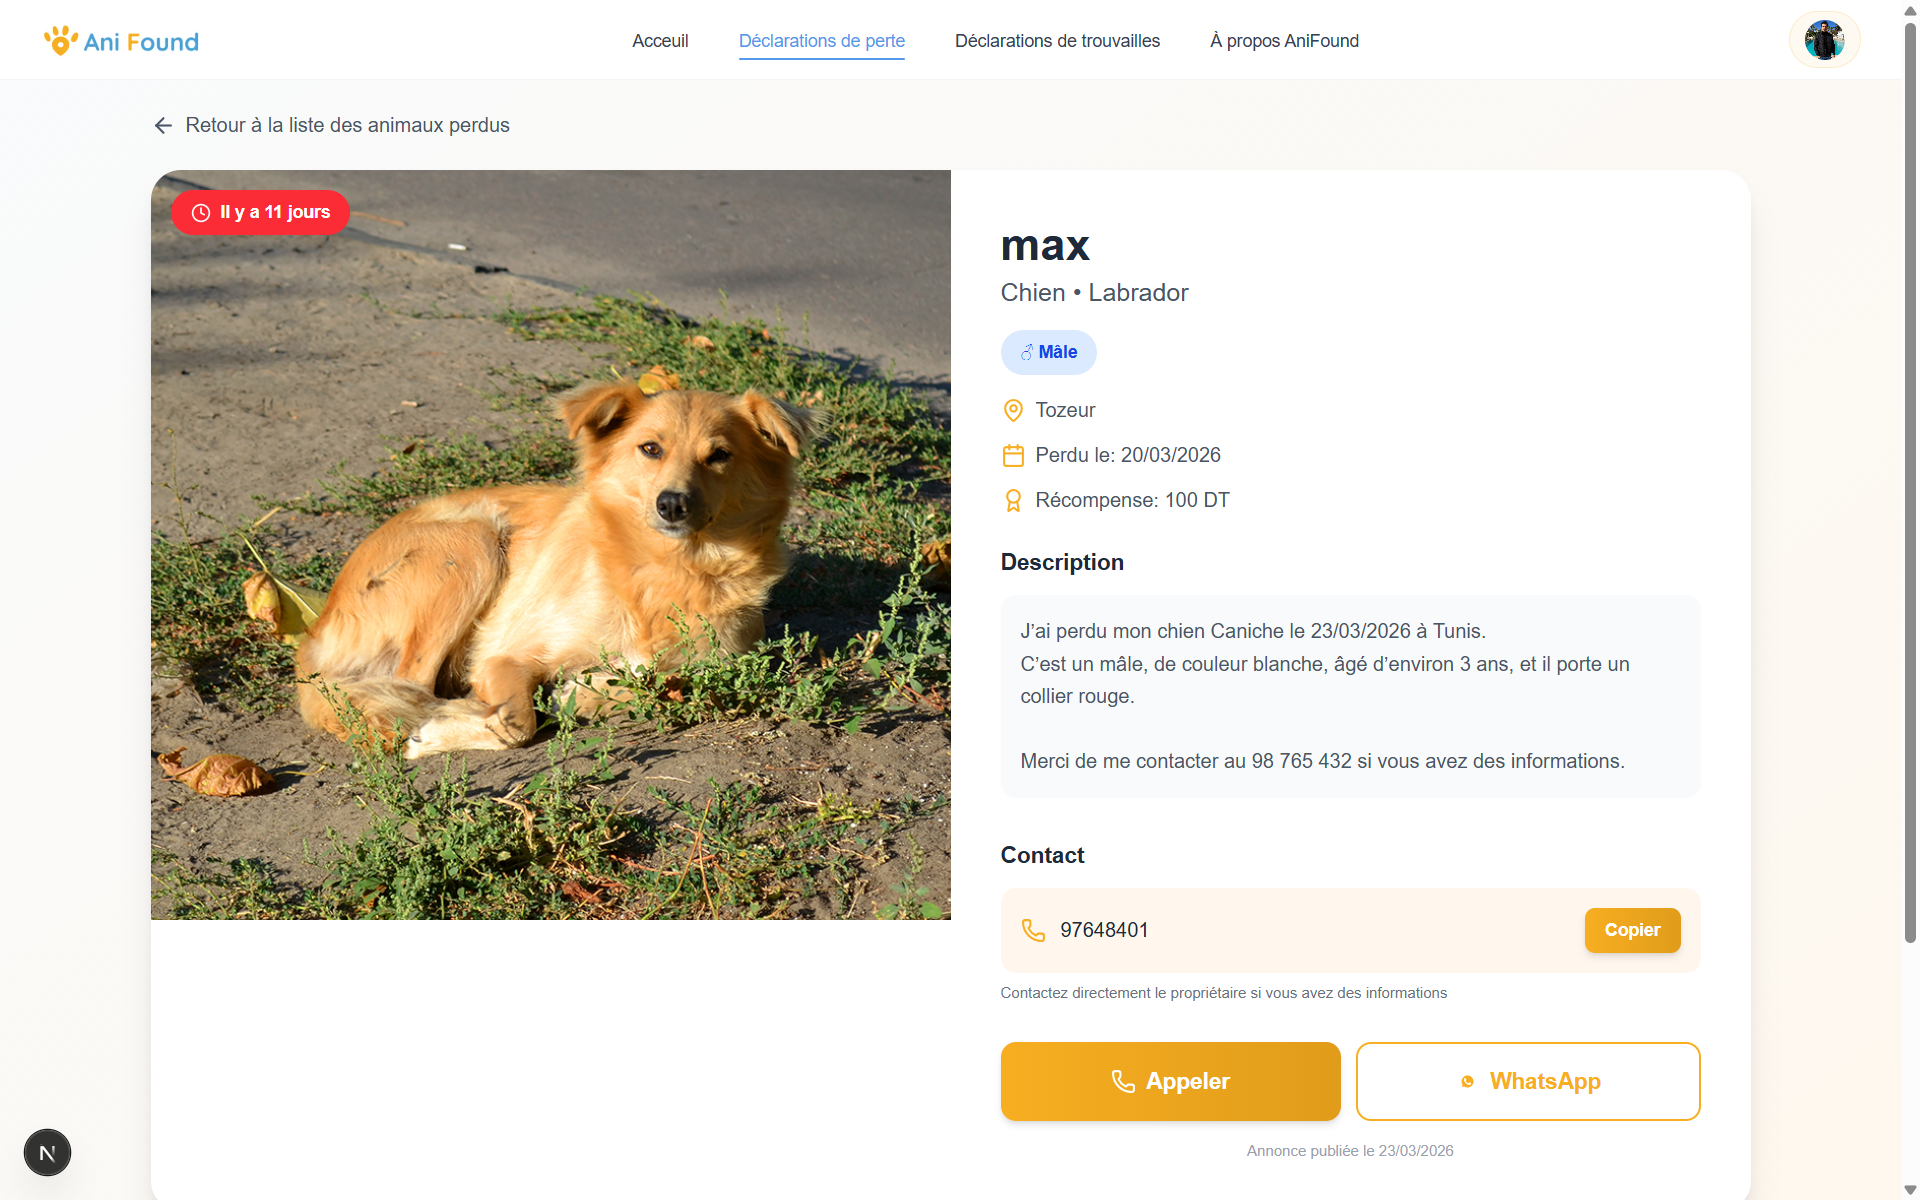
\includegraphics[width=0.77\textwidth]{images/details perte.png}
    \caption{Interface de détails d’une déclaration de perte}
    \label{fig:details_perte}
\end{figure}  

\subsubsection{Interface de l’espace AniFound et gestion du profil}

La figure \ref{fig:espace_anifound_profil} illustre l’espace utilisateur AniFound ainsi que la gestion du profil.

\begin{figure}[h!]
    \centering
    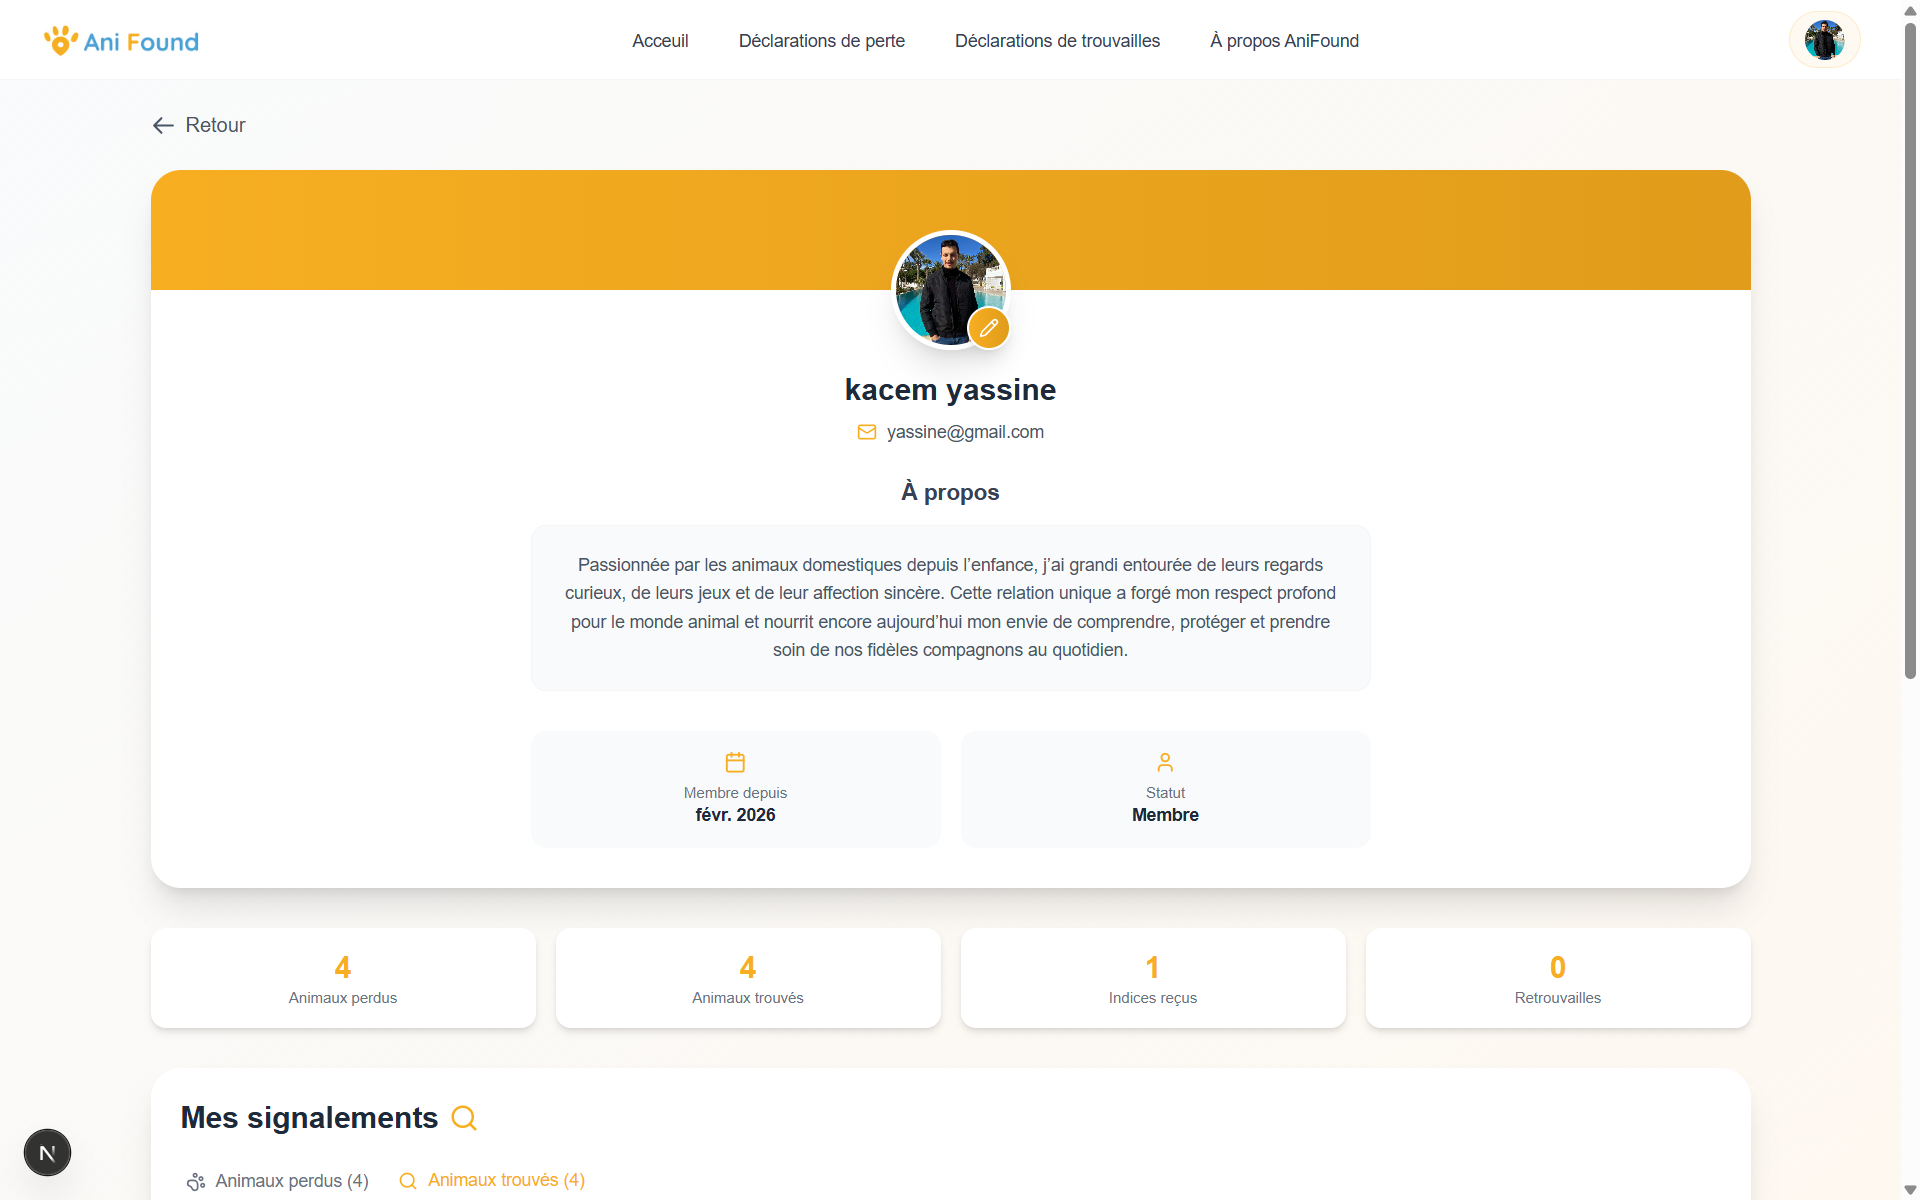
\includegraphics[width=0.77\textwidth]{images/espace anifound profil.png}
    \caption{Interface de l’espace AniFound et gestion du profil}
    \label{fig:espace_anifound_profil}
\end{figure}

\newpage 

\subsubsection{Interface de gestion de mes déclarations de perte et de trouvaille}

La figure \ref{fig:mes_signalements} illustre la gestion des déclarations personnelles de perte et de trouvaille.

\begin{figure}[h!]
    \centering
    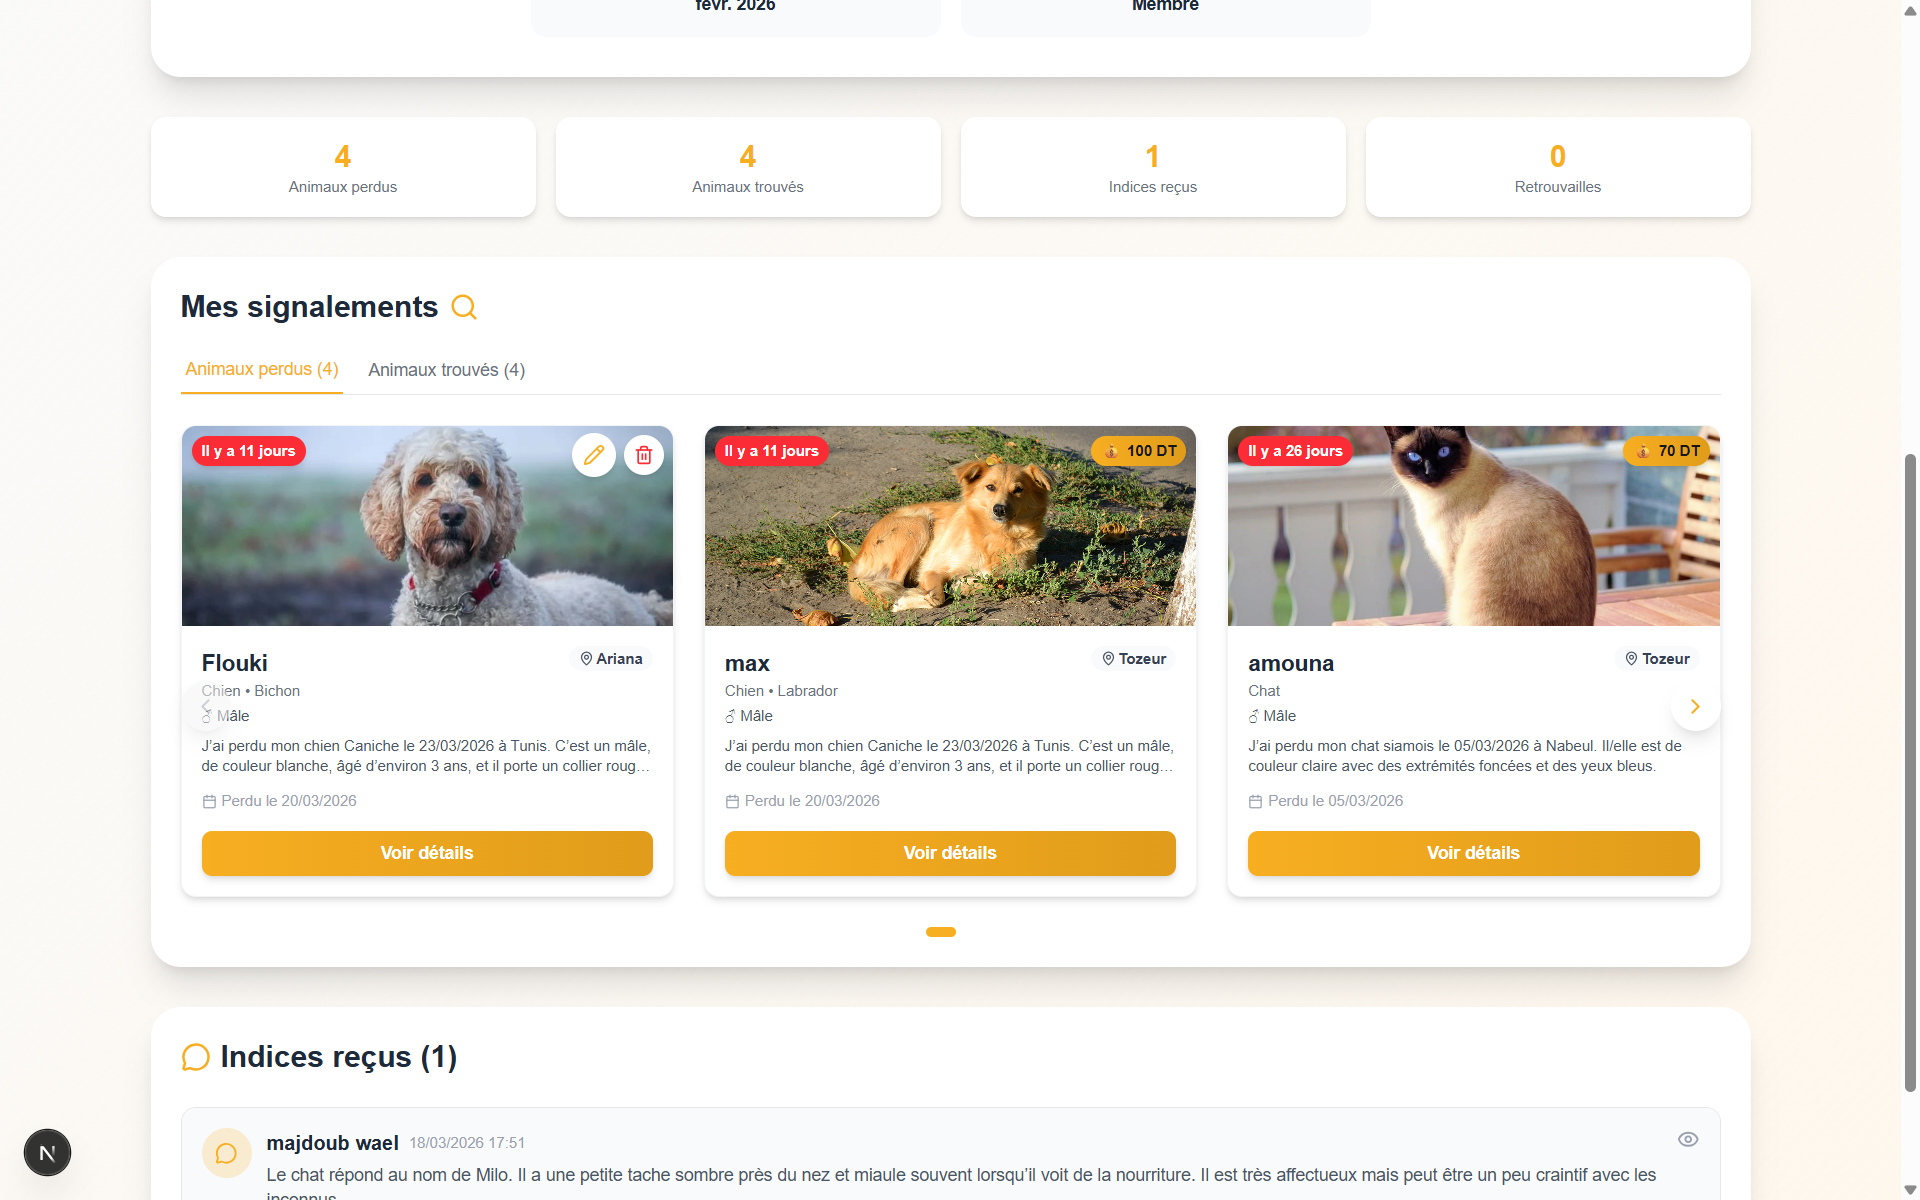
\includegraphics[width=0.87\textwidth]{images/mes signalements.png}
    \caption{Interface de gestion de mes déclarations de perte et de trouvaille}
    \label{fig:mes_signalements}
\end{figure} 

\subsubsection{Interfaces de modification et suppression d’une déclaration de perte ou de trouvaille}

La figure \ref{fig:modif_suppression_declaration} illustre les interfaces de modification et de suppression d’une déclaration.

\begin{figure}[h!]
    \centering
    
    \begin{minipage}{0.51\textwidth}
        \centering
        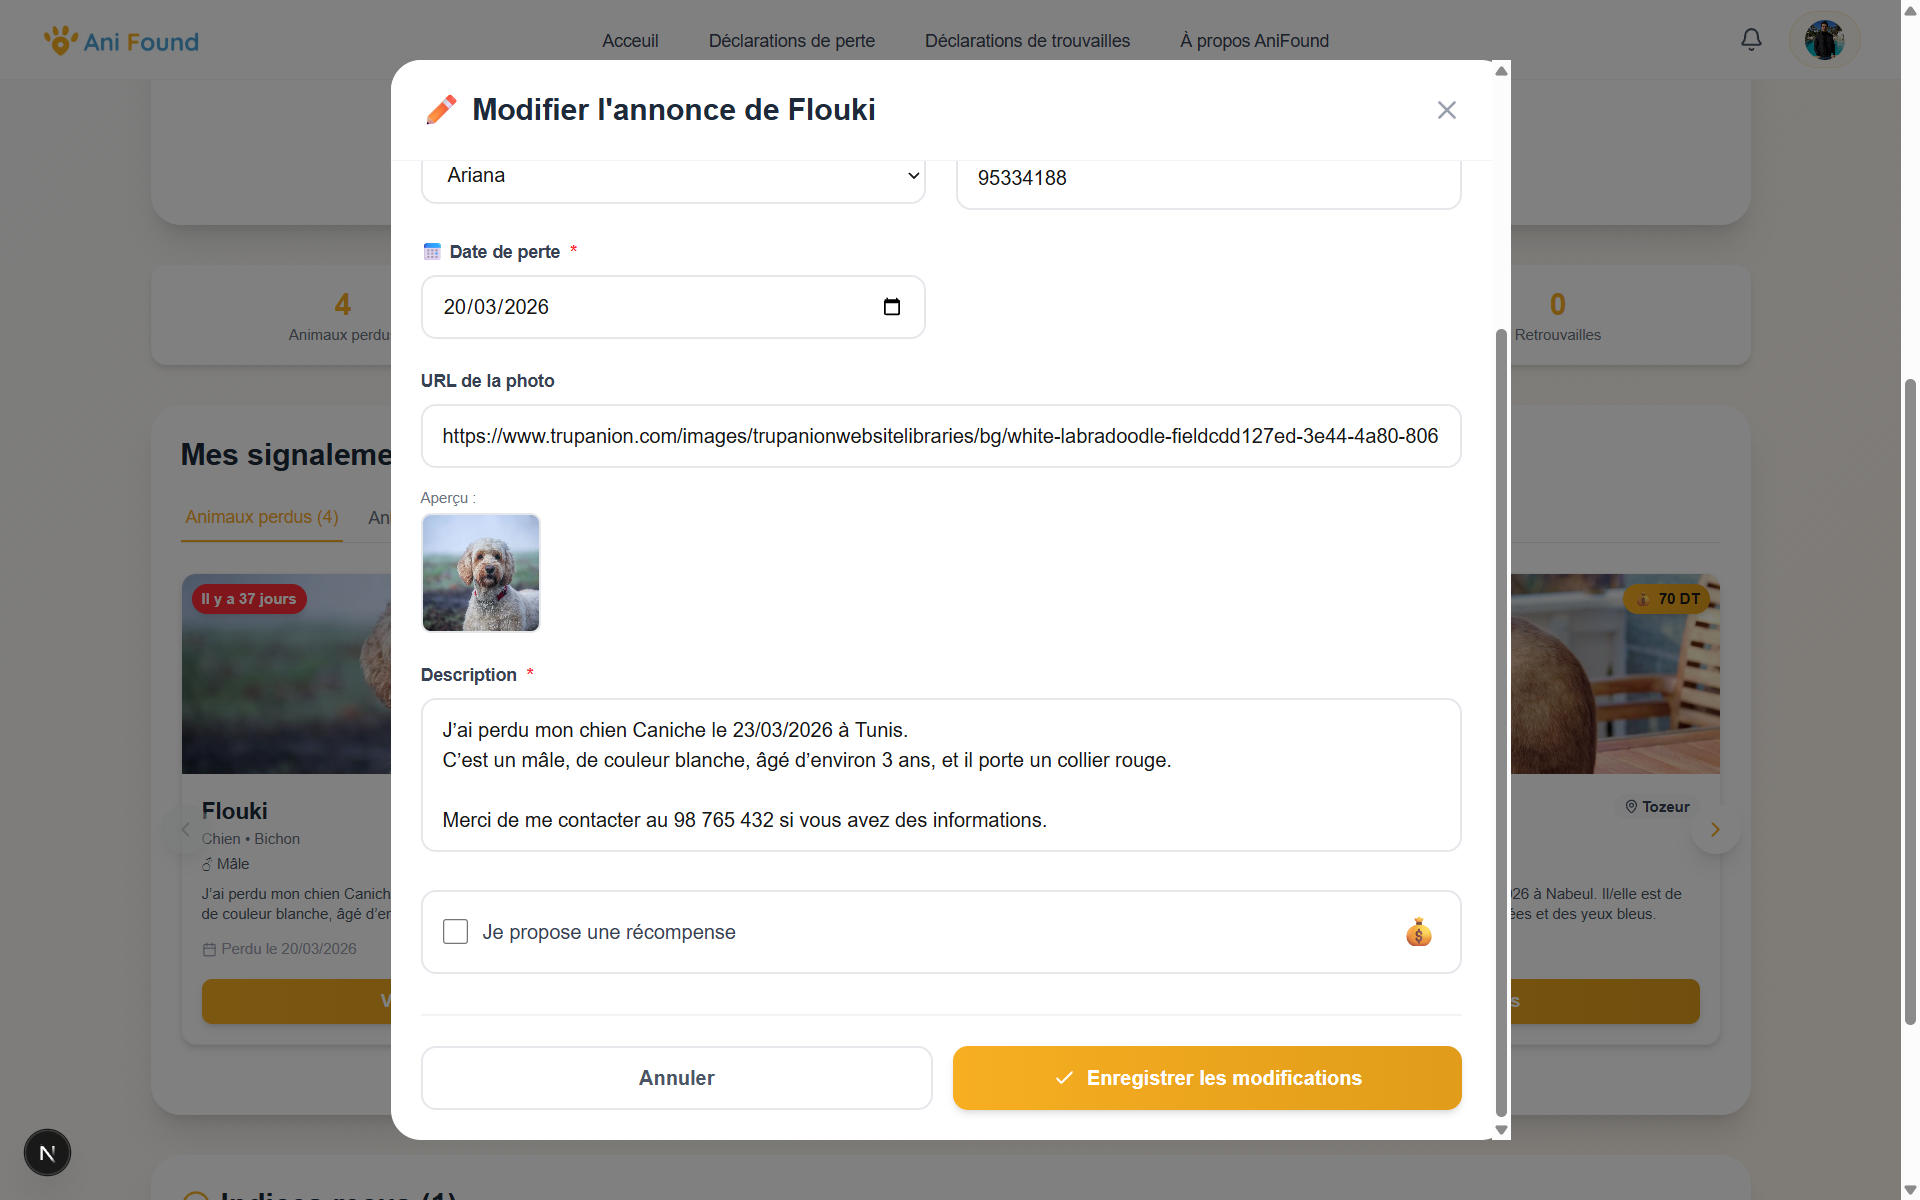
\includegraphics[width=0.77\textwidth]{images/modifer declaration.png}
        \caption{Interface de modification d’une déclaration de perte ou de trouvaille}
        \label{fig:modif_declaration}
    \end{minipage}
    \hfill
    \begin{minipage}{0.48\textwidth}
        \centering
        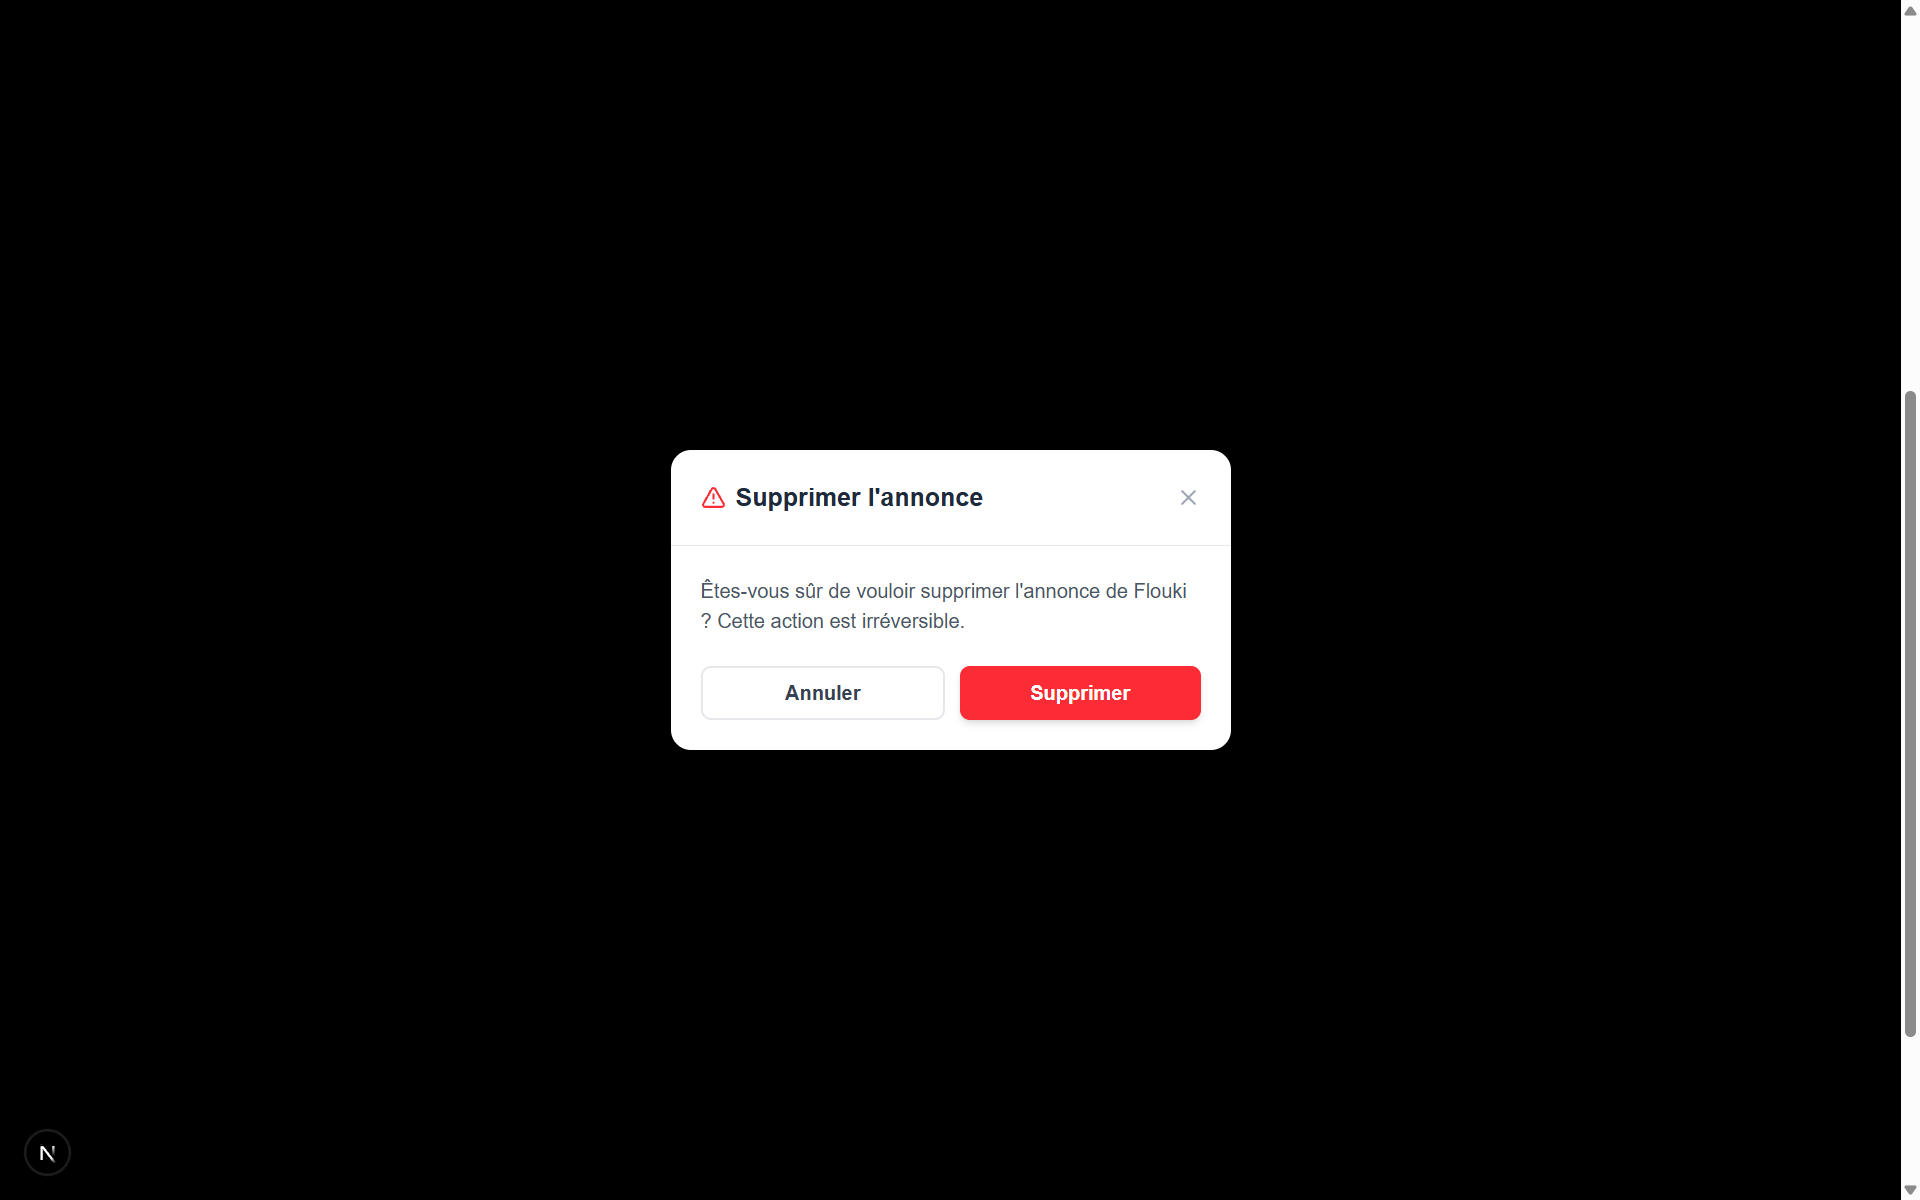
\includegraphics[width=0.77\textwidth]{images/suppression decalaration.png}
        \caption{Interface de suppression d’une déclaration de perte ou de trouvaille}
        \label{fig:suppression_declaration}
    \end{minipage}

\end{figure} 

\newpage 

\subsubsection{Interface des notifications reçues}

La figure \ref{fig:notifications_anifound} illustre une notification reçue concernant un indice lié à une déclaration de trouvaille.

\begin{figure}[h!]
    \centering
    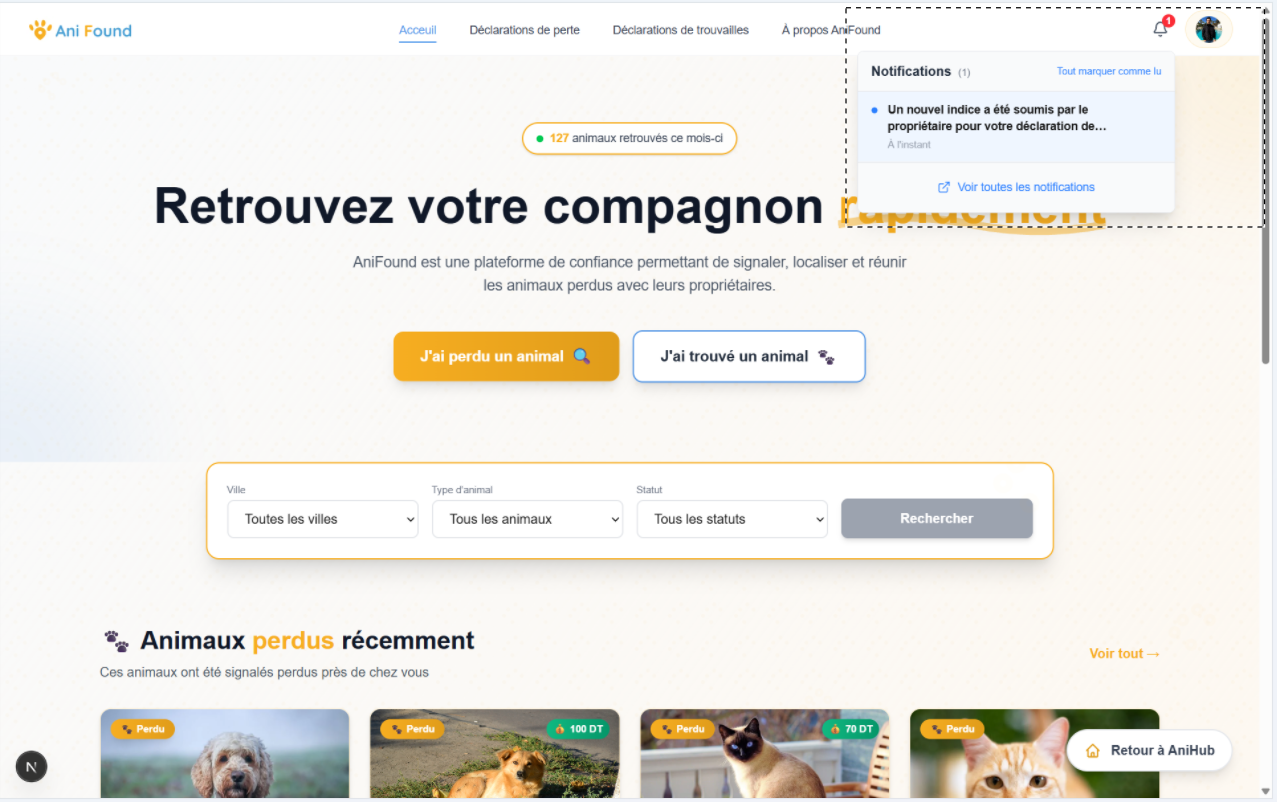
\includegraphics[width=0.77\textwidth]{images/notif anifound.png}
    \caption{Interface des notifications reçues}
    \label{fig:notifications_anifound}
\end{figure}

\subsubsection{Interface des indices reçus pour une déclaration de trouvaille}

La figure \ref{fig:indices_recus} illustre un indice reçu pour une déclaration de trouvaille.

\begin{figure}[h!]
    \centering
    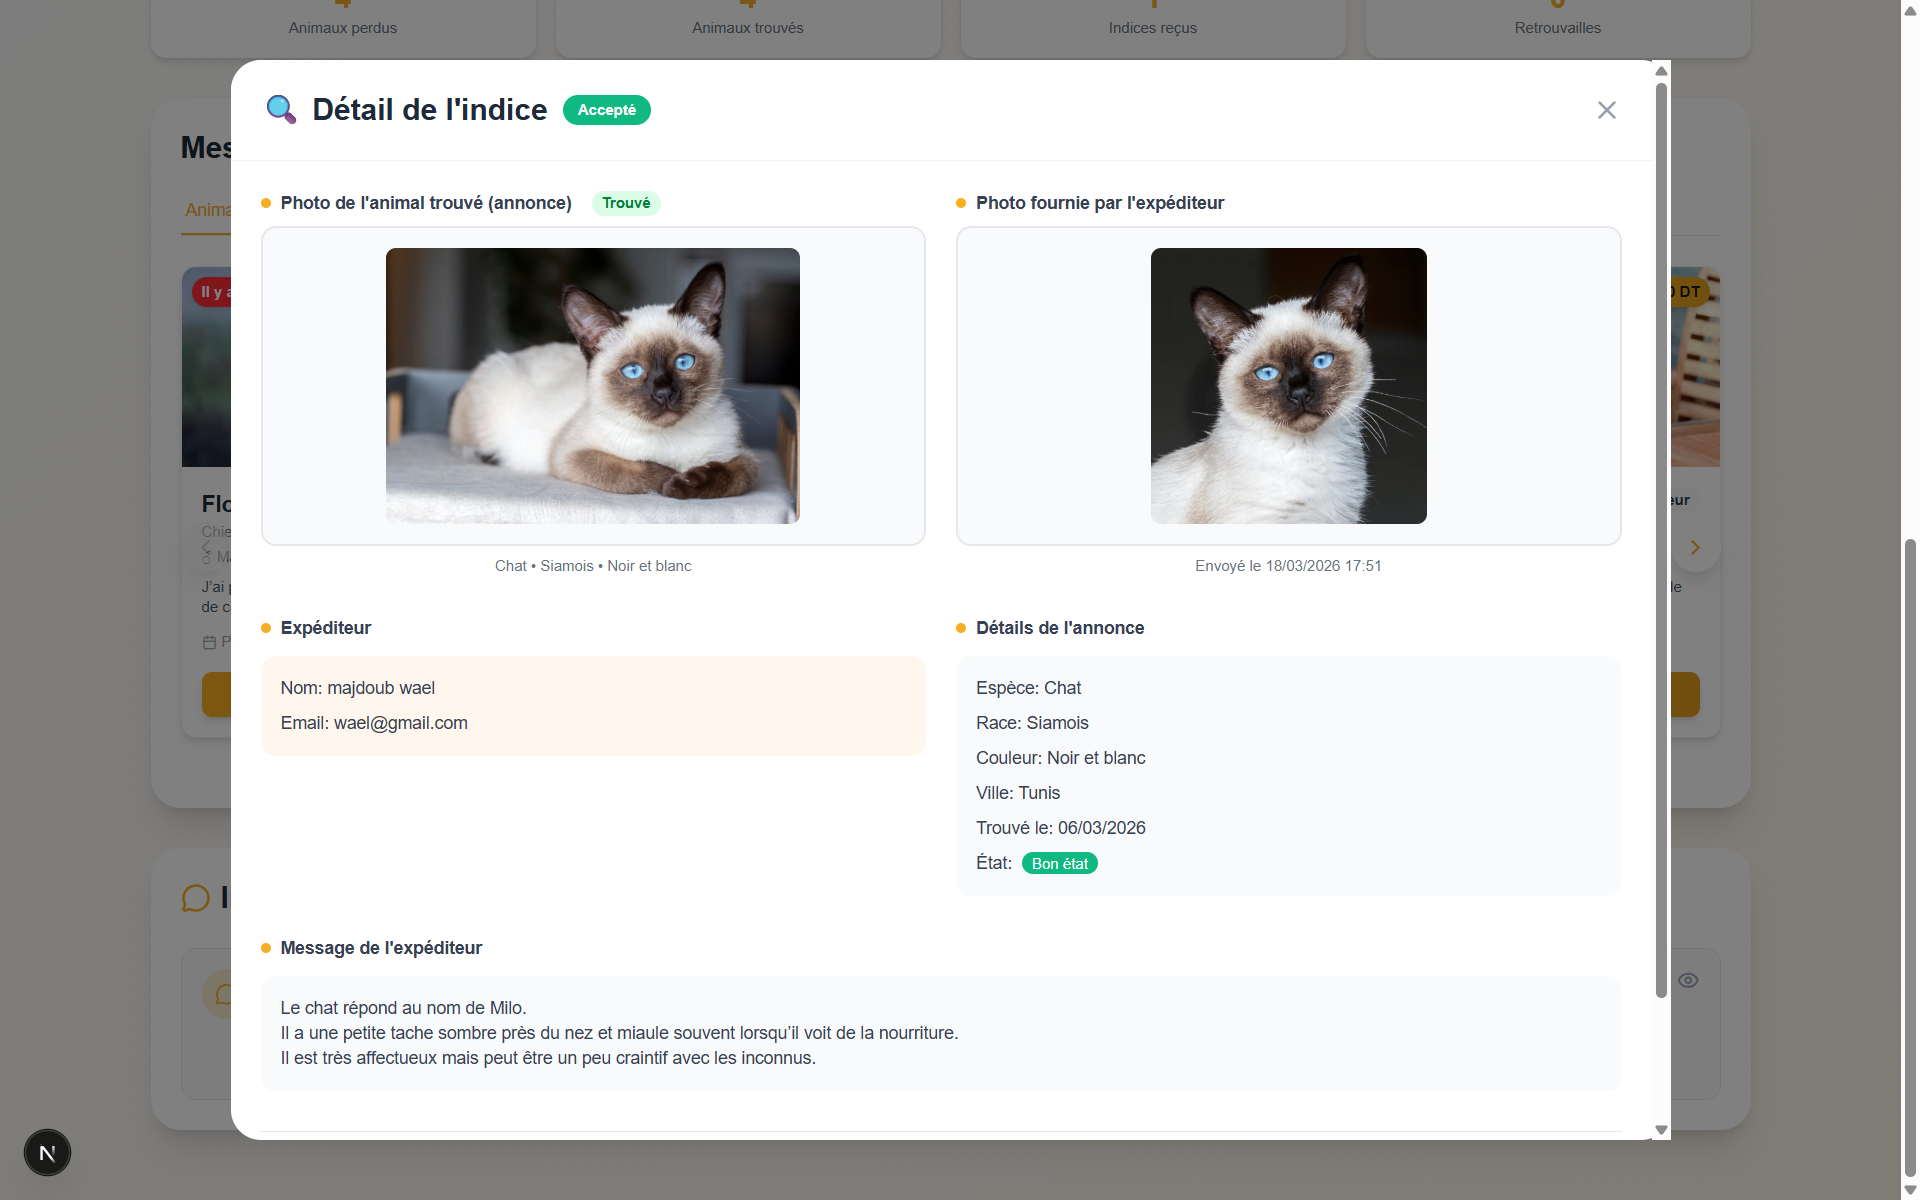
\includegraphics[width=0.77\textwidth]{images/indice recu.png}
    \caption{Interface des indices reçus pour une déclaration de trouvaille}
    \label{fig:indices_recus}
\end{figure}

\newpage
\section{Conclusion}

Ce chapitre a permis de présenter la première release du projet AniHub. Cette release contient trois sprints : le sprint 1 consacré à l’authentification et à l’administration, ainsi que les sprints 2 et 3 dédiés aux modules AniMatch et AniFound. Nous avons détaillé les différentes fonctionnalités développées à travers ces sprints, en mettant en évidence les besoins fonctionnels, la conception ainsi que la réalisation des principales interfaces utilisateur. Cette phase a contribué à mettre en place les principaux mécanismes d’authentification, de mise en relation et de gestion des animaux perdus ou trouvés au sein du système. 


\chapter{Release 2 : AniHub partie 2 } 
\label{chap:4}
\section{Introduction} 

La deuxième release vise l’enrichissement et la finalisation technique de la plateforme . Elle est réalisée à travers trois sprints :
\begin{itemize}
    \item \textbf{Sprint 4 : Module AniMarket}
    \item \textbf{Sprint 5 : Module AniCare}
    \item \textbf{Sprint 6 : Conteneurisation, CI/CD, Déploiement et Monitoring}
\end{itemize}

\section{Sprint 4 : Module AniMarket}   
\begin{figure}[H]
    \centering
    
\includegraphics[width=3.5cm]{images/animarket.png}
    \caption{Logo du module AniMarket}
    \label{fig:logo-animarket}
\end{figure}
Ce sprint, d’une durée de \textbf{3 semaines}, est dédié au module AniMarket, permettant la gestion des annonces d’animaux (vente directe et enchères) et les interactions entre utilisateurs. 
\subsection{Sprint backlog}  
\begin{longtable}{|p{1cm}|p{5cm}|p{8cm}|p{1cm}|}
\caption{Sprint Backlog du Sprint 4}
\label{tab:sprint4-backlog} \\ 
\hline
\rowcolor{coloranimarket}
\textbf{ID} & \textbf{User Story} & \textbf{Tâches} & \textbf{Effort} \\
\hline
\endfirsthead

\hline
\rowcolor{coloranimarket}
\textbf{ID} & \textbf{User Story} & \textbf{Tâches} & \textbf{Effort} \\
\hline
\endhead

% ===================== US1 =====================
\multirow{5}{2cm}{US1}
& \multirow{5}{5cm}{En tant qu’utilisateur, je veux consulter la liste des animaux à vendre afin de découvrir les annonces disponibles}
& Conception de l’interface (Figma) & 1 j \\
\cline{3-4}
& & API récupération animaux & 1.5 j \\
\cline{3-4}
& & Interface enchères et ventes directes  & 1.5 j \\
\cline{3-4}
& & Filtrage , tri et recherche & 1 j \\
\cline{3-4}
& & Intégration frontend/backend & 1.5 j \\
\hline

% ===================== US2 =====================
\multirow{3}{2cm}{US2}
& \multirow{3}{5cm}{En tant qu’utilisateur, je veux proposer une offre sur une enchère}
& API offres et enchères & 1 j \\
\cline{3-4}
& & Intégration interface des offres & 1 j \\
\cline{3-4}
& & Tests & 0.5 j \\
\hline

% ===================== US3 =====================
\multirow{6}{2cm}{US3}
& \multirow{6}{5cm}{En tant qu’utilisateur, je veux gérer mes notifications afin d’être informé des interactions sur mes activités}
& Analyse besoins notifications & 1 j \\
\cline{3-4}
& & Développement microservice Notifications & 1.5 j \\
\cline{3-4}
& & Intégration RabbitMQ avec le microservice AniMarket et le microservice notifications & 1.5 j \\
\cline{3-4}
& & Création événements (offres, enchères, wishlist) & 1 j \\
\cline{3-4}
& & Interface notifications frontend & 1 j \\
\cline{3-4}
& & Marquer comme lu / non lu & 0.5 j \\
\hline

% ===================== US4 =====================
\multirow{4}{2cm}{US4}
& \multirow{4}{5cm}{En tant que vendeur, je veux gérer mes animaux à vendre afin de maintenir mes annonces à jour}
& API CRUD animaux & 1.5 j \\
\cline{3-4}
& & Interface espace animarket & 1 j \\
\cline{3-4}
& & Gestion des annonces (frontend) & 1 j \\
\cline{3-4}
& & Tests & 0.5 j \\
\hline

% ===================== US5 =====================
\multirow{3}{2cm}{US5}
& \multirow{3}{5cm}{En tant qu’utilisateur, je veux gérer ma wishlist}
& API wishlist & 1 j \\
\cline{3-4}
& & Ajout / suppression animal & 0.5 j \\
\cline{3-4}
& & Interface ma wishlist & 1 j \\
\hline

% ===================== US6 =====================
\multirow{3}{2cm}{US6}
& \multirow{3}{5cm}{En tant que vendeur, je veux gérer les offres reçues}
& API gestion offres & 1 j \\
\cline{3-4}
& & Accepter / refuser offre & 1 j \\
\cline{3-4}
& & Tests & 0.5 j \\
\hline

% ===================== US7 =====================
\multirow{3}{2cm}{US7}
& \multirow{3}{5cm}{En tant qu’utilisateur, je veux commenter et noter un animal}
& API commentaires et avis & 1 j \\
\cline{3-4}
& & Interface frontend & 1 j \\
\cline{3-4}
& & Tests & 0.5 j \\
\hline

% ===================== US8 =====================
\multirow{3}{2cm}{US8}
& \multirow{3}{5cm}{En tant qu’utilisateur, je veux discuter avec le vendeur}
& Analyse & 0.5 j \\
\cline{3-4}
& & Intégration bouton WhatsApp & 0.5 j \\
\cline{3-4}
& & Génération lien wa.me & 0.5 j \\
\hline

\end{longtable}
\newpage
\subsection{Diagramme des cas d’utilisation du sprint 4} 
Dans cette section, nous présentons le diagramme des cas d’utilisation du Sprint 4, dédié au module AniMarket.  
Ce diagramme illustre les principales interactions entre l’utilisateur et le système, notamment la gestion des annonces, des enchères et des ventes directes.  
La figure ci-dessous représente le diagramme des cas d’utilisation correspondant : 


\begin{figure}[H]
    \centering
  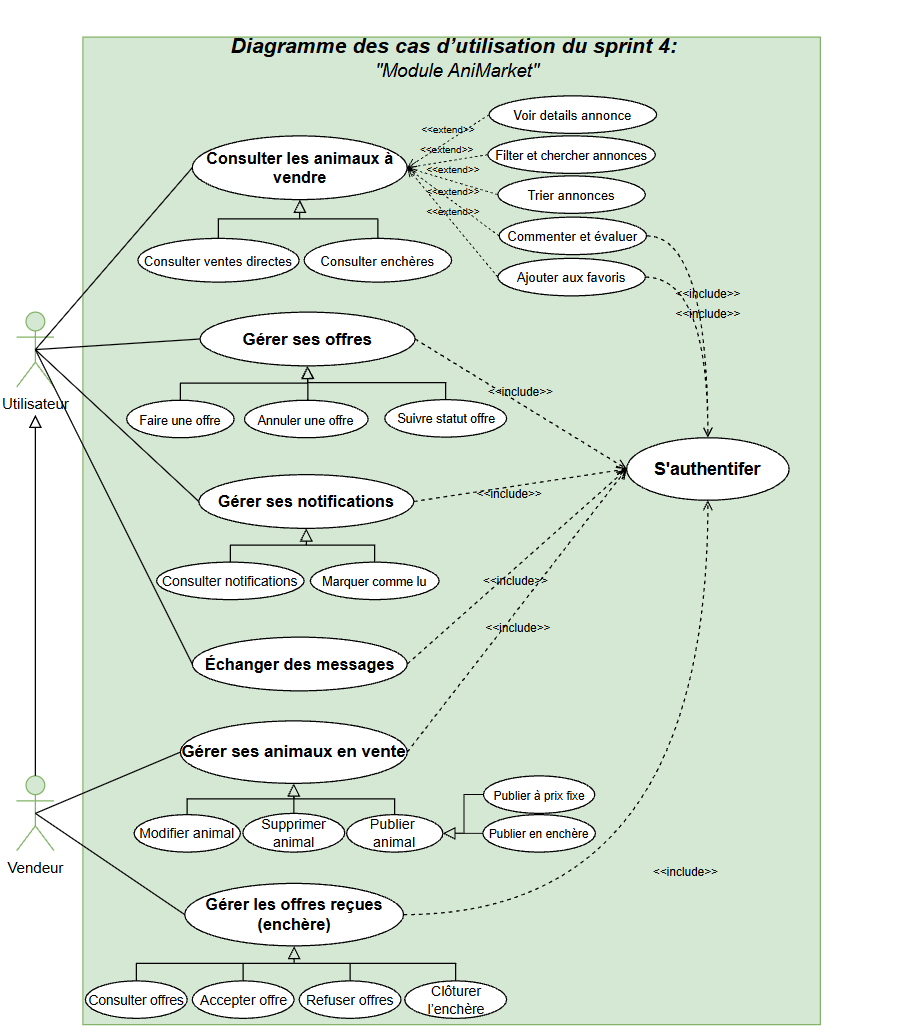
\includegraphics[width=0.98\linewidth, height=18.5cm, keepaspectratio]{images/usecase animarket.png}
    \caption{Diagramme des cas d’utilisation du sprint 4}
    \label{fig:usecase-sprint4}
\end{figure} 
\newpage
\subsection{Descriptions textuelles des cas d’utilisation du sprint 4}  
  Dans cette section, nous présentons les descriptions textuelles des cas d’utilisation du Sprint 4 afin de détailler le comportement du système pour chaque fonctionnalité du module AniMarket. 
  \subsubsection{Description textuelle du cas d’utilisation « Consulter les animaux à vendre (prix fixe ou enchères) »}

Le tableau ci-dessous illustre le cas d’utilisation Consulter les animaux à vendre, lors de la recherche et de la consultation des annonces disponibles (prix fixe ou enchères) :

\begin{longtable}{|c|p{11cm}|}
\caption{Description textuelle du cas d’utilisation "Consulter les animaux à vendre"}
\label{tab:consulter_animaux_vente} \\
\hline
\cellcolor{coloranimarket} \textbf{Nom du cas d'utilisation } & Consulter les animaux à vendre (prix fixe ou enchères) \\
\hline
\cellcolor{coloranimarket} \textbf{Acteurs} & Utilisateur \\
\hline
\cellcolor{coloranimarket} \textbf{Description } & Tout utilisateur peut consulter les annonces d’animaux disponibles à la vente directe ou aux enchères dans le module AniMarket. \\
\hline
\cellcolor{coloranimarket} \textbf{Pré-condition } &  Accès à la plateforme sans authentification requise. \\
\hline
\cellcolor{coloranimarket} \textbf{Post-condition } & L’utilisateur a consulté la liste des animaux à vendre. \\
\hline
\cellcolor{coloranimarket} \textbf{Scénario nominal } & 
\begin{enumerate} 

\item L’utilisateur accède à la plateforme AniHub.
\item L’utilisateur choisit le module AniMarket.
\item Le système redirige l’utilisateur vers la page d'acceuil du  module AniMarket.
\item L’utilisateur choisit entre « Vente directe » ou « Enchères ».
\item Le système affiche la liste des animaux correspondante.
\item L’utilisateur peut filtrer eyt chercher les annonces selon différents critères (prix , espèce , race ...).
\item Le système affiche les résultats filtrés.
\item L’utilisateur sélectionne une annonce.
\item Le système affiche les détails de l’annonce. 
\item L’utilisateur peut ajouter un animal à sa wishlist.
\item Le système ajoute l’animal à la wishlist de l’utilisateur.
\item L’utilisateur peut commenter et laisser un avis sur l’animal.
\item Le système enregistre le commentaire et l’avis de l’utilisateur.
\end{enumerate} \\
\hline
\end{longtable}

\newpage
\subsubsection{Description textuelle du cas d’utilisation « Gérer ses offres envoyées »}

Le tableau ci-dessous illustre le cas d’utilisation Gérer ses offres envoyées, permettant à l’utilisateur de faire et annuler une offre sur une enchère :
\begin{longtable}{|c|p{11cm}|}
\caption{Description textuelle du cas d’utilisation "Gérer ses offres envoyées"}
\label{tab:gerer_offres} \\
\hline
\cellcolor{coloranimarket} \textbf{Nom du cas d'utilisation } & Gérer ses offres envoyées \\
\hline
\cellcolor{coloranimarket} \textbf{Acteurs} & Utilisateur \\
\hline
\cellcolor{coloranimarket} \textbf{Description } & L’utilisateur peut consulter les offres d’une enchère, faire une nouvelle offre et annuler une offre déjà envoyée. \\
\hline
\cellcolor{coloranimarket} \textbf{Pré-condition } & L’utilisateur doit accéder aux détails d’une enchère. \\
\hline
\cellcolor{coloranimarket} \textbf{Post-condition } & Les offres sont ajoutées, supprimées avec succées. \\
\hline
\cellcolor{coloranimarket} \textbf{Scénario nominal } &
\begin{enumerate}
\item L’utilisateur accède à la plateforme AniHub.
\item L’utilisateur choisit le module AniMarket.
\item Le système redirige l’utilisateur vers la page d’accueil du module AniMarket.
\item L’utilisateur choisit la catégorie Enchères.
\item Le système affiche la liste des animaux en enchères.
\item L’utilisateur consulte les détails d’une enchère.
\item Selon l’action de l’utilisateur :

\begin{itemize}

\item \textbf{Cas 1 : Publication d’une offre}
\begin{enumerate}
\item L’utilisateur saisit un montant et envoie une offre.
\item Le système vérifie et enregistre l’offre.
\item Le système confirme l’envoi de l’offre.
\end{enumerate}


\item \textbf{Cas 2 : Suppression d’une offre}
\begin{enumerate}
\item Le système supprime l’offre et confirme l’annulation.
\item Si l’offre supprimée était la plus élevée, le système met à jour le prix de l’enchère.
\end{enumerate}

\end{itemize}

\end{enumerate} \\
\hline
\cellcolor{coloranimarket} \textbf{Scénario alternatif :} &
\begin{itemize}
\item Si l’utilisateur saisit une offre inférieure ou égale à la dernière offre, le système affiche une erreur.
\item Si l’utilisateur annule une offre qui n’est pas la plus élevée, le système supprime l’offre sans impact sur le prix actuel de l’enchère.
\end{itemize} \\
\hline
\end{longtable} 
\newpage 


\subsubsection{Description textuelle du cas d’utilisation « Gérer mes animaux à vendre »}
Le tableau ci-dessous illustre le cas d’utilisation « Gérer mes animaux à vendre » dans le module AniMarket :
\begin{longtable}{|c|p{11cm}|}
\caption{Description textuelle du cas d'utilisation "Gérer mes animaux à vendre"}
\label{tab:gerer_animaux_vente} \\
\hline
\cellcolor{coloranimarket}\textbf{Nom du cas d'utilisation } & Gérer mes animaux à vendre \\
\hline
\cellcolor{coloranimarket}\textbf{Acteurs} & Vendeur \\
\hline
\cellcolor{coloranimarket}\textbf{Description } & Le vendeur peut publier, modifier et supprimer ses annonces d’animaux dans AniMarket (vente directe ou enchères). \\
\hline
\cellcolor{coloranimarket}\textbf{Pré-condition } & L’utilisateur doit être authentifié en tant que vendeur. \\
\hline
\cellcolor{coloranimarket}\textbf{Post-condition } & Les annonces sont correctement publiées, mises à jour ou supprimées. \\
\hline

\cellcolor{coloranimarket}\textbf{Scénario nominal } &
\begin{enumerate}
\item L’utilisateur se connecte à son compte
\item L’utilisateur sélectionne le module AniMarket.
\item Le système redirige l’utilisateur vers AniMarket.
\item L’utilisateur accède à son <<espace animarket>>.
\item Le système affiche la liste de ses animaux à vendre.

\item \textbf{Cas publication :}
\begin{itemize}
\item L’utilisateur clique sur « Publier un animal ».
\item Le système affiche un formulaire de création.
\item L’utilisateur vente directe ou enchère,  saisit les informations et valide la publication.
\item Le système enregistre l’annonce et l’affiche.
\end{itemize}

\item \textbf{Cas modification :}
\begin{itemize}
\item L’utilisateur et clique sur « Modifier ».
\item Le système affiche le formulaire pré-rempli.
\item L’utilisateur modifie les informations.
\end{itemize}

\item \textbf{Cas suppression :}
\begin{itemize}
\item L’utilisateur clique sur « Supprimer ».
\item Le système demande confirmation.
\item L’utilisateur confirme la suppression.
\item Le système supprime l’annonce.
\end{itemize}

\item Le système met à jour et affiche un message de succès.
\end{enumerate} \\
\hline

\cellcolor{coloranimarket}\textbf{Scénario alternatif :} &
\begin{itemize}
\item En cas d’erreur lors de la publication ou modification, le système affiche un message d’erreur.
\item En cas d’annulation, l’annonce est conservée.
\end{itemize} \\
\hline

\end{longtable} 




\newpage 

\subsection{Diagramme des classes du sprint 4}  
Dans cette section, nous présentons le diagramme de classes du Sprint 4, qui regroupe l’ensemble des classes du module AniMarket.

La figure ci-dessous illustre le diagramme de classes correspondant :
\begin{figure}[H]
    \centering
    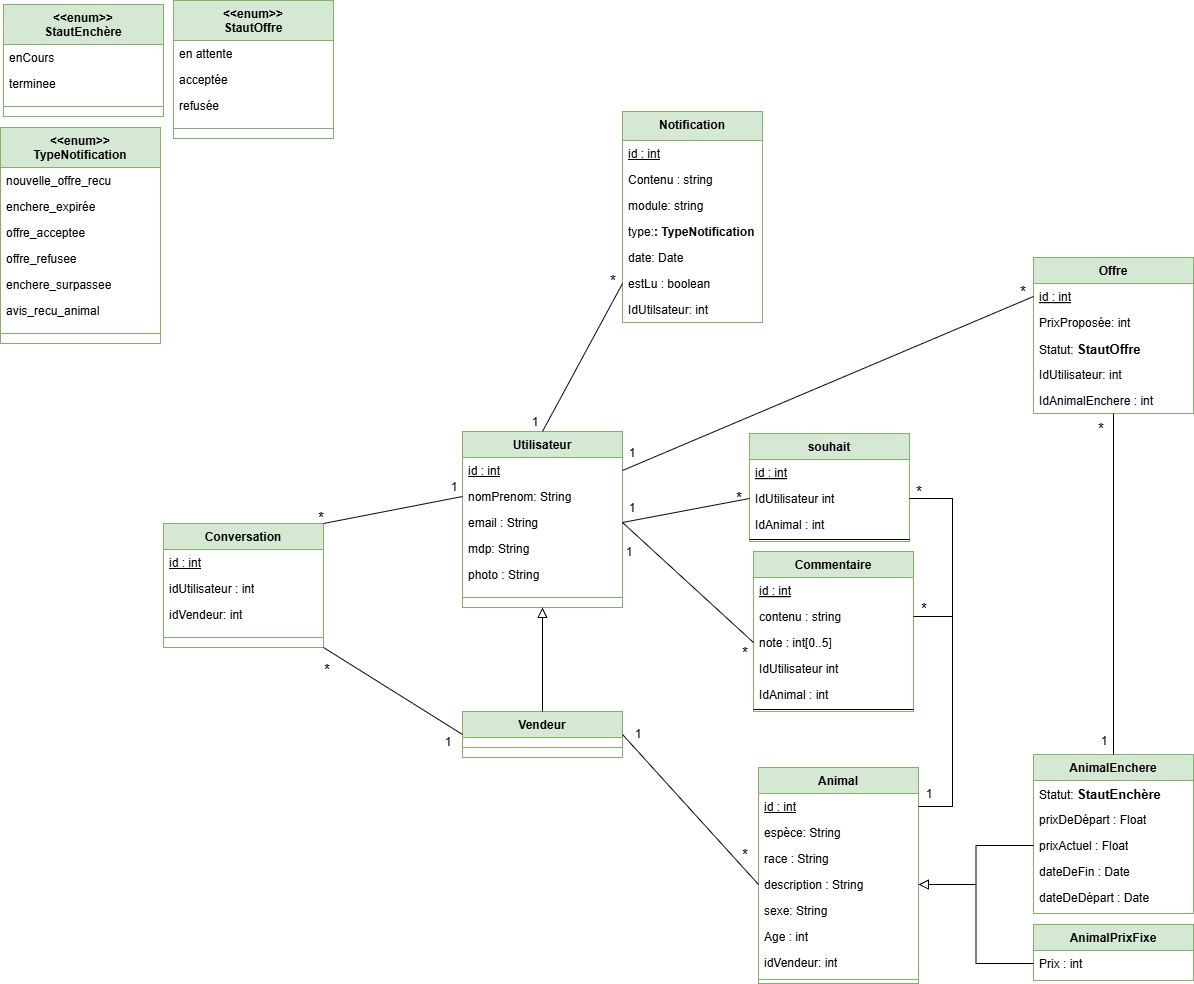
\includegraphics[width=1\textwidth, height=20cm, keepaspectratio]{images/class diagram animarket.png}
    \caption{Diagramme de classes du sprint 4}
    \label{fig:class_diagram_animarket}
\end{figure} 
\newpage 
\subsection{Diagrammes de séquence du sprint 4}

Dans cette section, nous présentons les diagrammes de séquence du quatrième sprint, illustrant les interactions entre les différents composants du système ainsi que le déroulement des principales fonctionnalités implémentées. 
\subsubsection{Diagramme de séquence : consultation des animaux à vendre}

Cette figure illustre les interactions de l’utilisateur avec le système pour consulter et filtrer les animaux disponibles à la vente, ainsi que les fonctionnalités associées telles que les commentaires, les favoris et l’envoi d’offres pour les enchères : 
\begin{figure}[H]
    \centering
    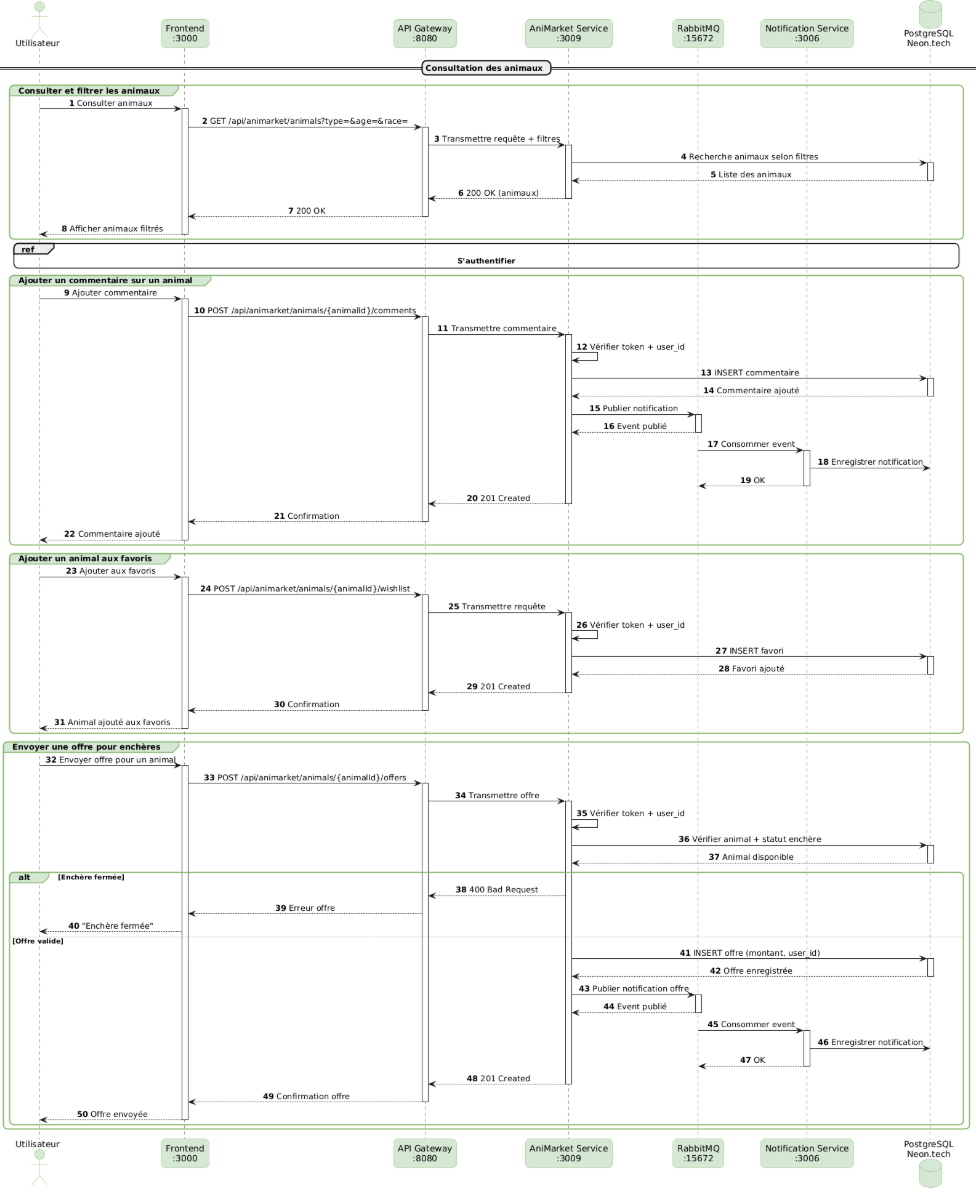
\includegraphics[width=0.75\textwidth]{images/consulter animaux animarket sq.png}
    \caption{Diagramme de séquence : consultation des animaux à vendre}
    \label{fig:animarket_consultation}
\end{figure} 
\newpage 
\subsubsection{Diagramme de séquence : gestion des animaux}

Cette figure illustre les interactions du vendeur avec le système pour la gestion de ses animaux, notamment l’ajout, la modification et la suppression : 

\begin{figure}[H]
    \centering
    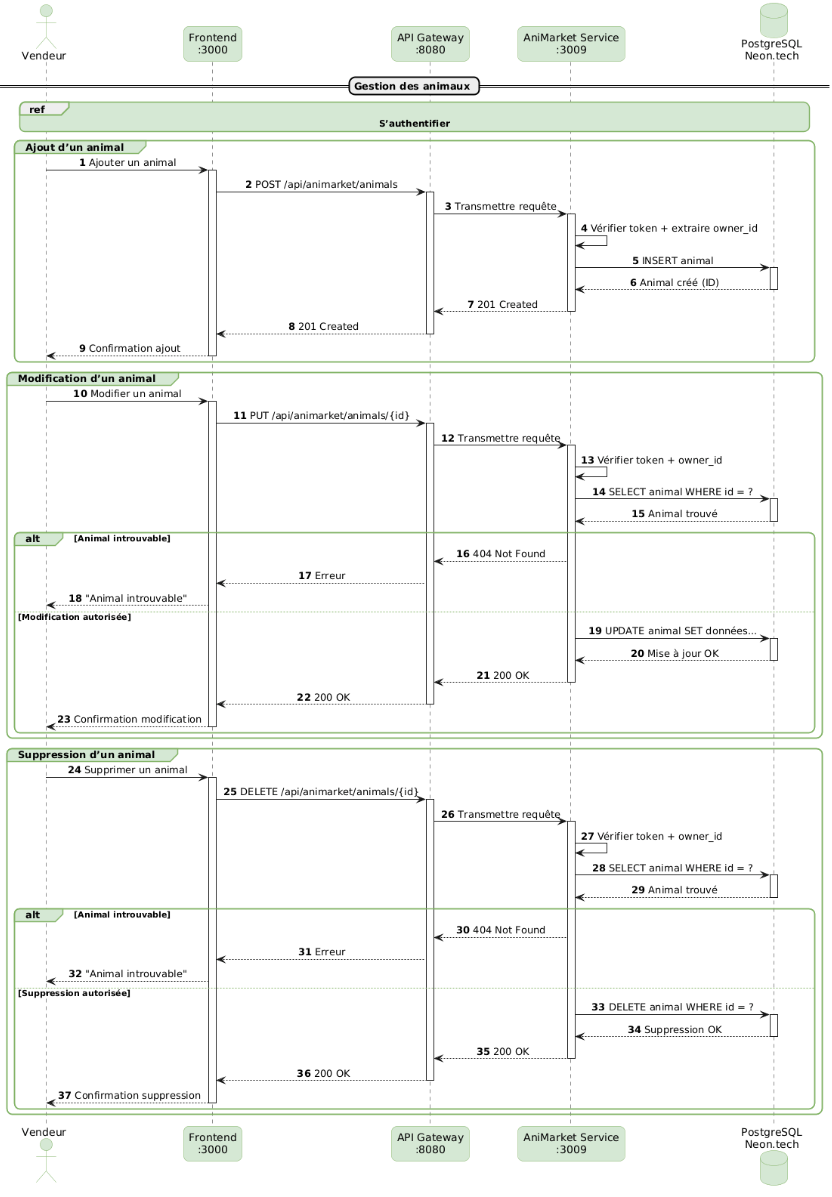
\includegraphics[width=0.78\textwidth]{images/gerer aimaux animarket sq.png}
    \caption{Diagramme de séquence : gestion des animaux}
    \label{fig:gestion_animaux}
\end{figure}





\newpage 
\subsection{Réalisation du sprint 4} 

\subsubsection{Menu principal de l’application AniHub et interface d’accueil AniMarket} 

Cette figure illustre le menu principal de l’application AniHub ainsi que l’interface d’accueil du module AniMarket : 

\begin{figure}[h!]
    \centering
    
    \begin{minipage}{0.48\textwidth}
        \centering
        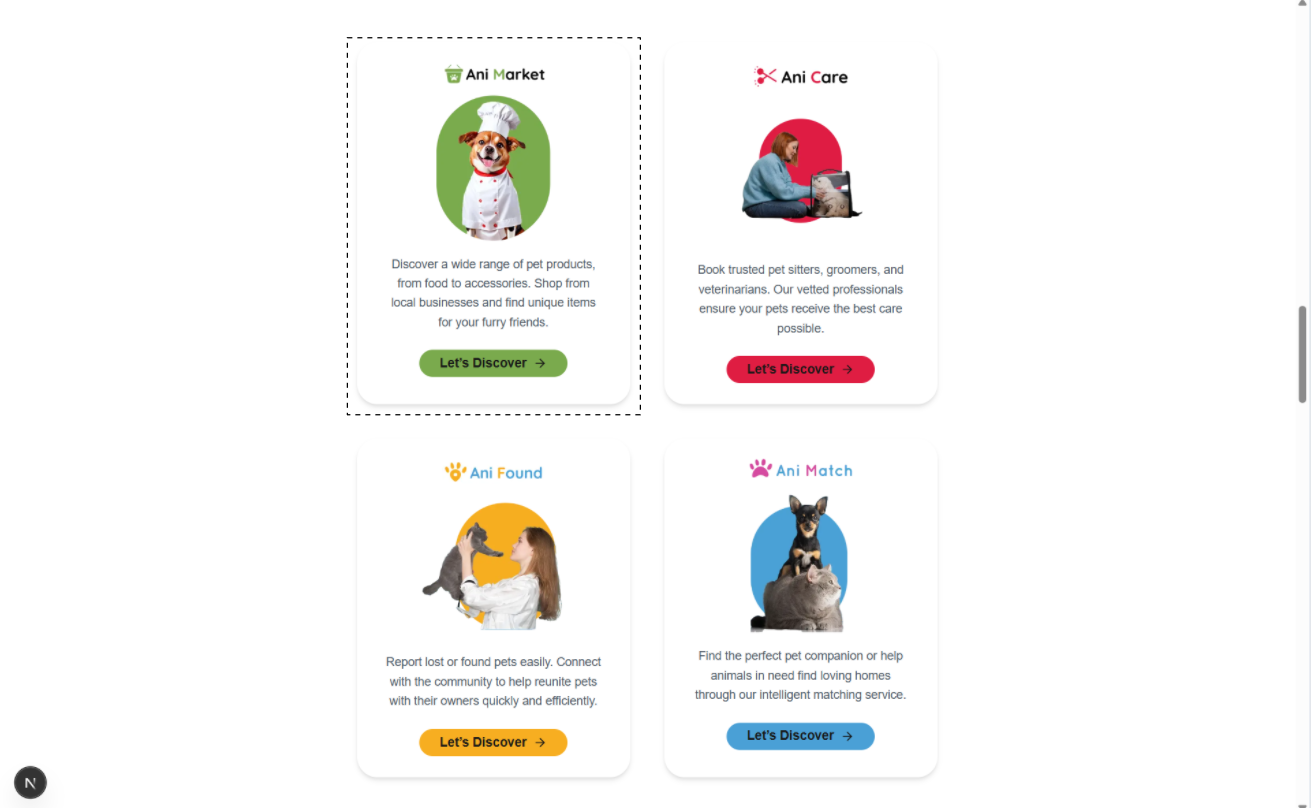
\includegraphics[width=0.85\textwidth]{images/menu animarket.png}
        \caption{Menu principal de l’application AniHub}
    \end{minipage}
    \hfill
    \begin{minipage}{0.48\textwidth}
        \centering
        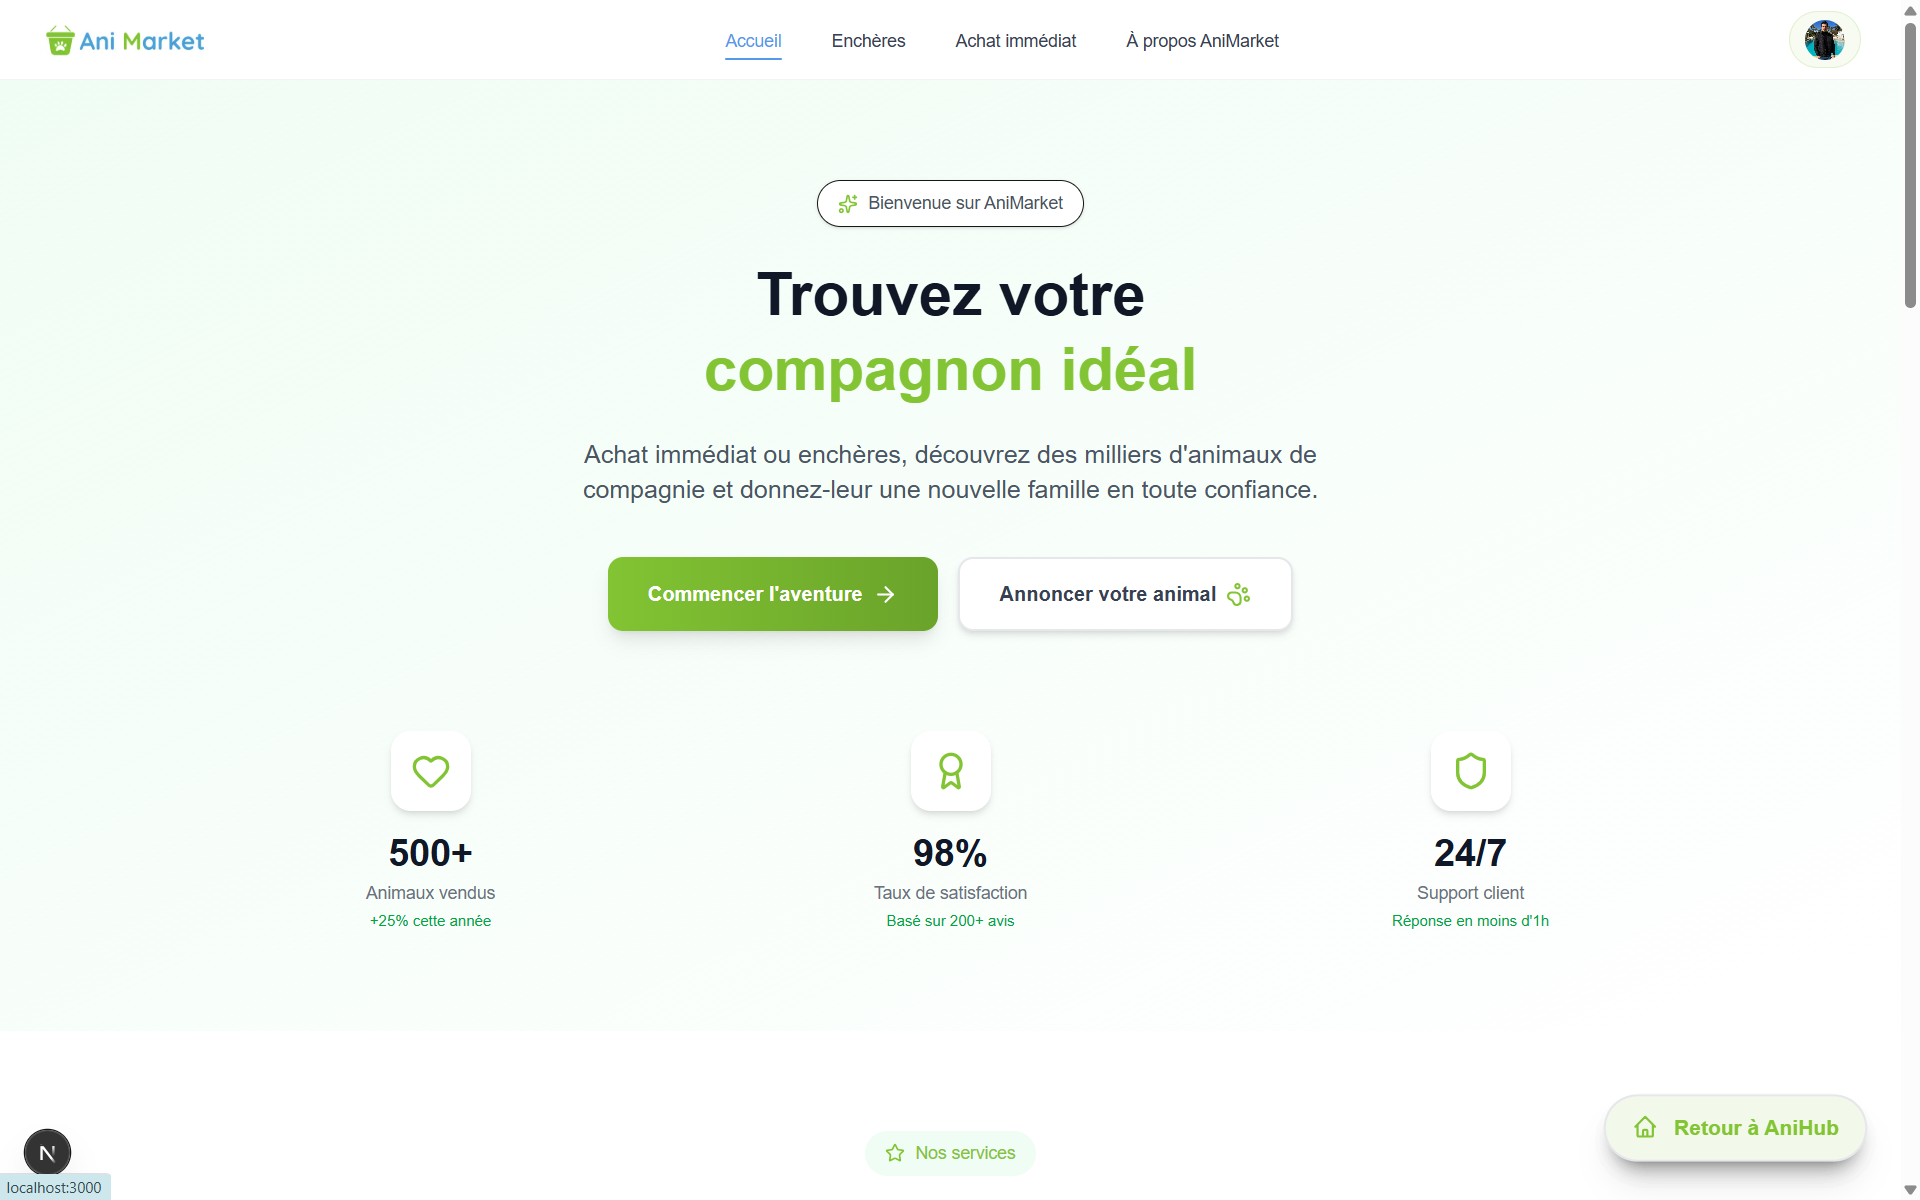
\includegraphics[width=0.85\textwidth]{images/home.png}
        \caption{Interface d’accueil AniMarket}
    \end{minipage}

\end{figure}   

\subsubsection{Interface d’annonce d’animal pour vente (enchère ou prix fixe)} 
La figure ci-dessous illustre l’interface d’annonce d’animal pour vente, où l’utilisateur peut choisir entre une enchère ou un prix fixe : 
\begin{figure}[h!]
    \centering
    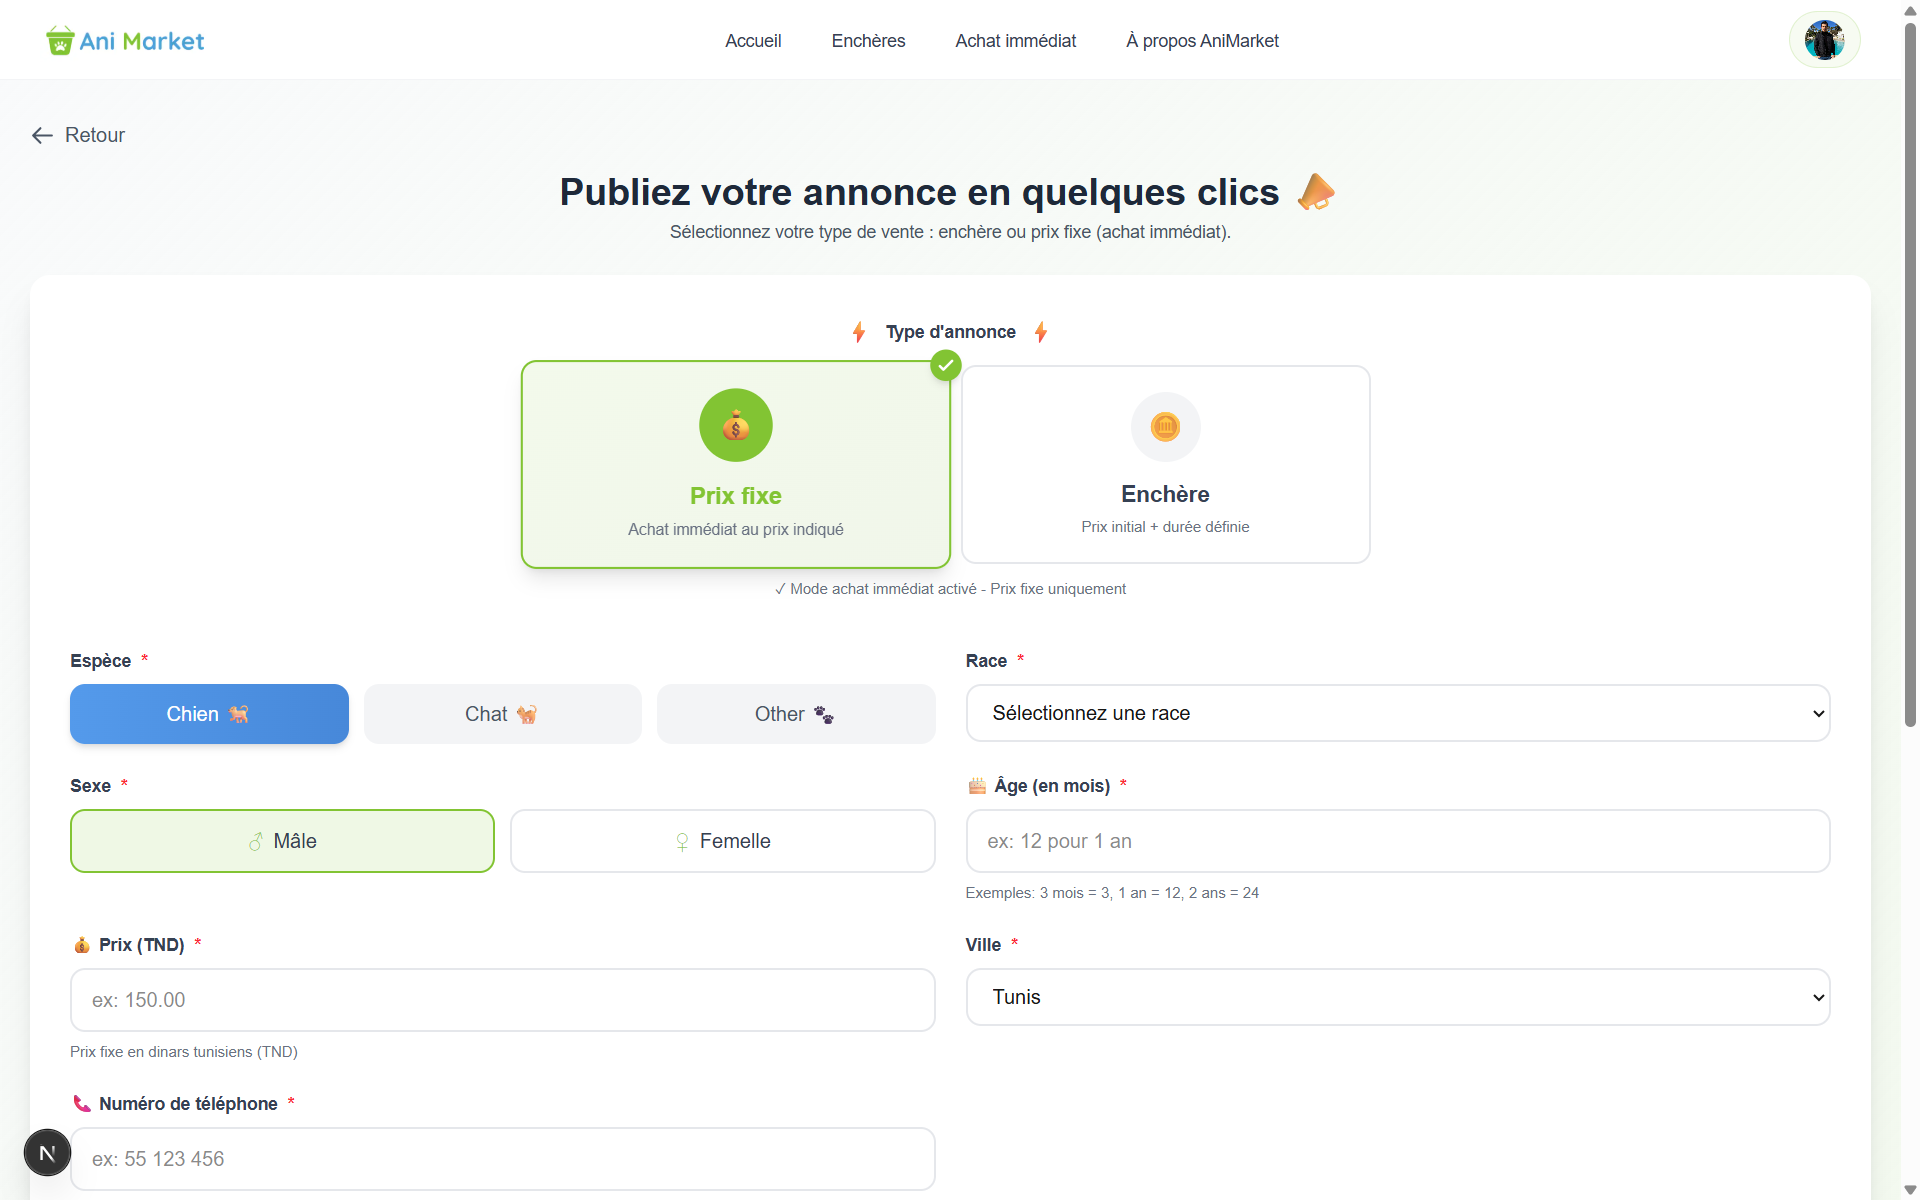
\includegraphics[width=0.77\textwidth]{images/annoncer animal.png}
    \caption{Interface d’annonce d’animal pour vente}
\end{figure}   

\newpage  
\subsubsection{Interface des achats immédiats (prix fixe)}

La figure ci-dessous illustre la page des achats immédiats (prix fixe) : 
\begin{figure}[h!]
    \centering
    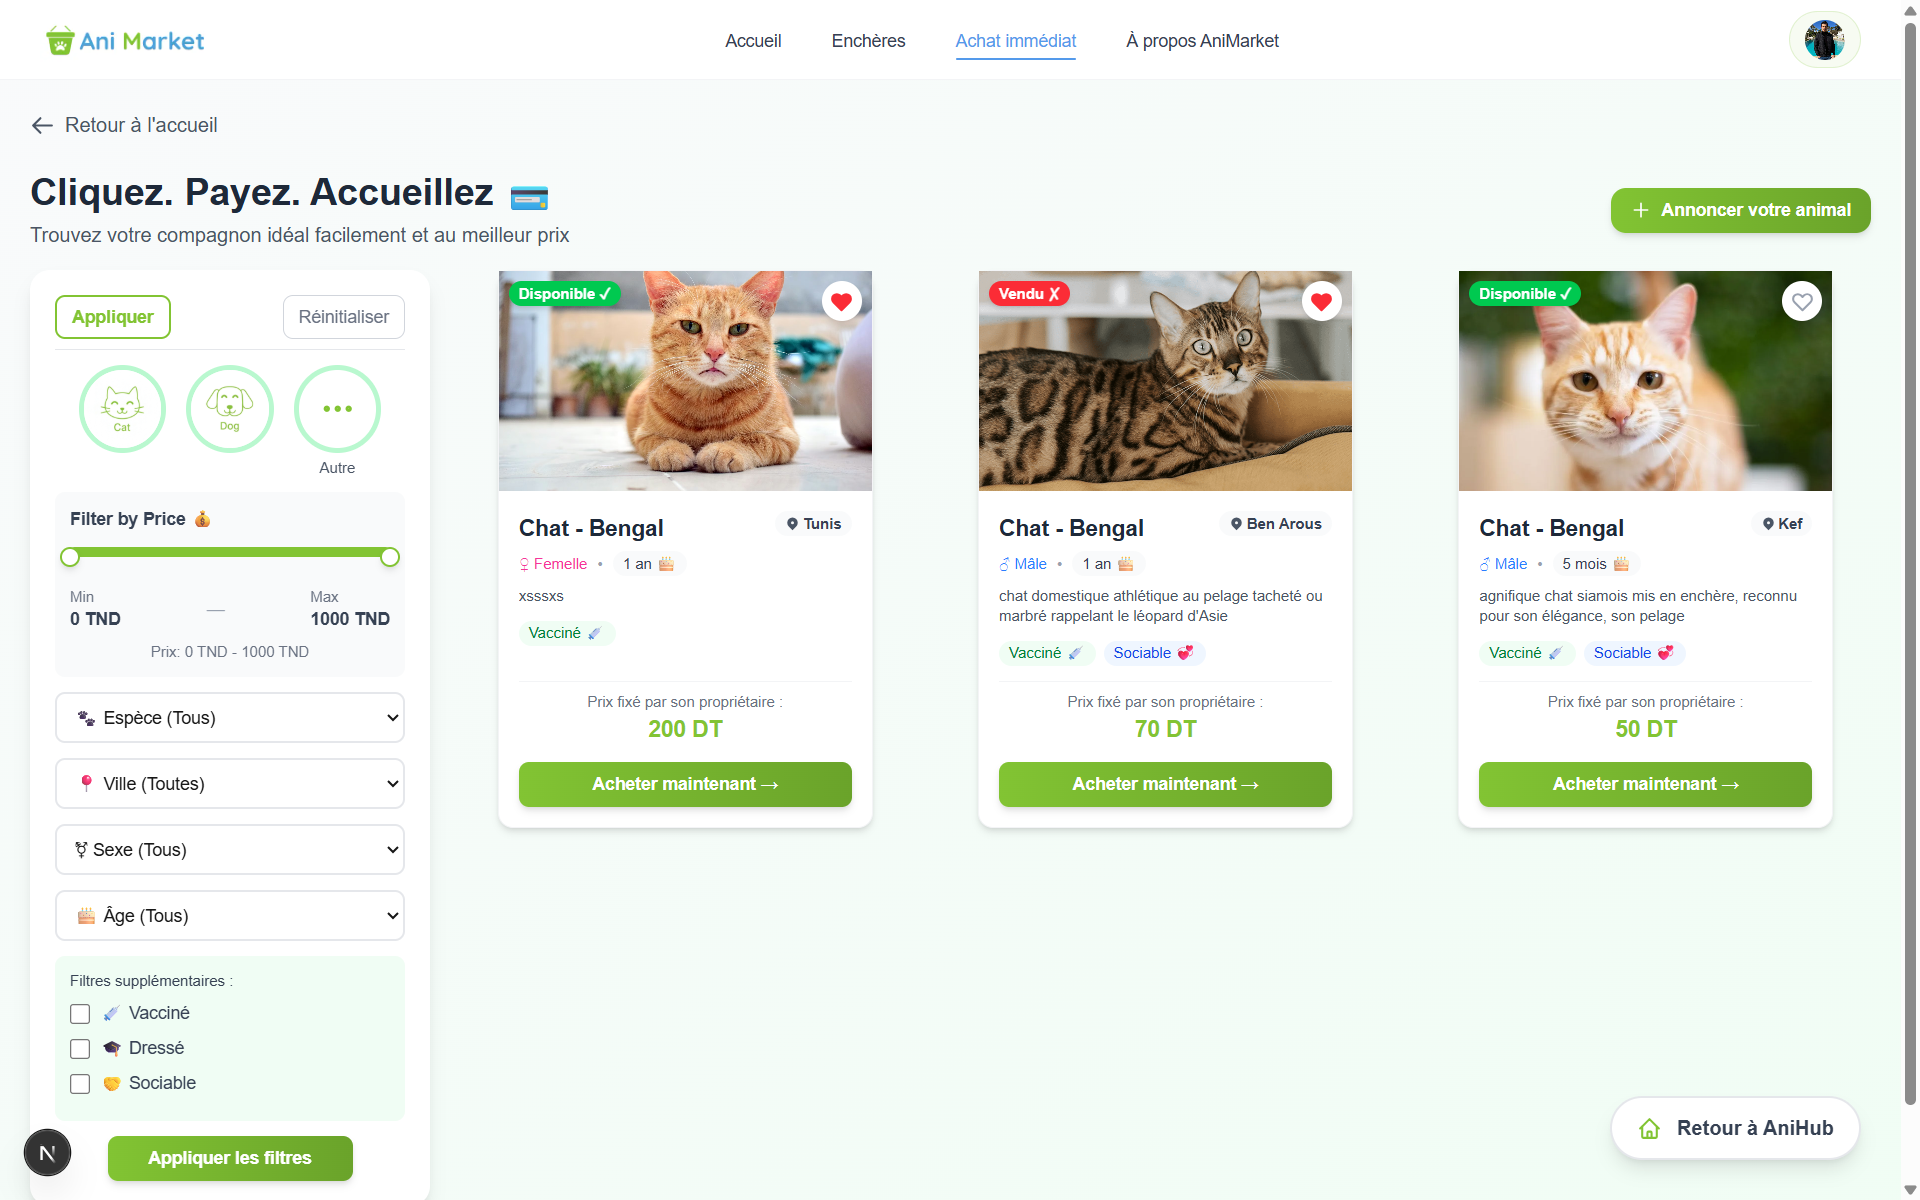
\includegraphics[width=0.77\textwidth]{images/page prix fixe.png}
    \caption{Interface des achats immédiats}
\end{figure}    


\subsubsection{Interface des enchères}

La figure ci-dessous illustre la page des enchères : 
\begin{figure}[h!]
    \centering
    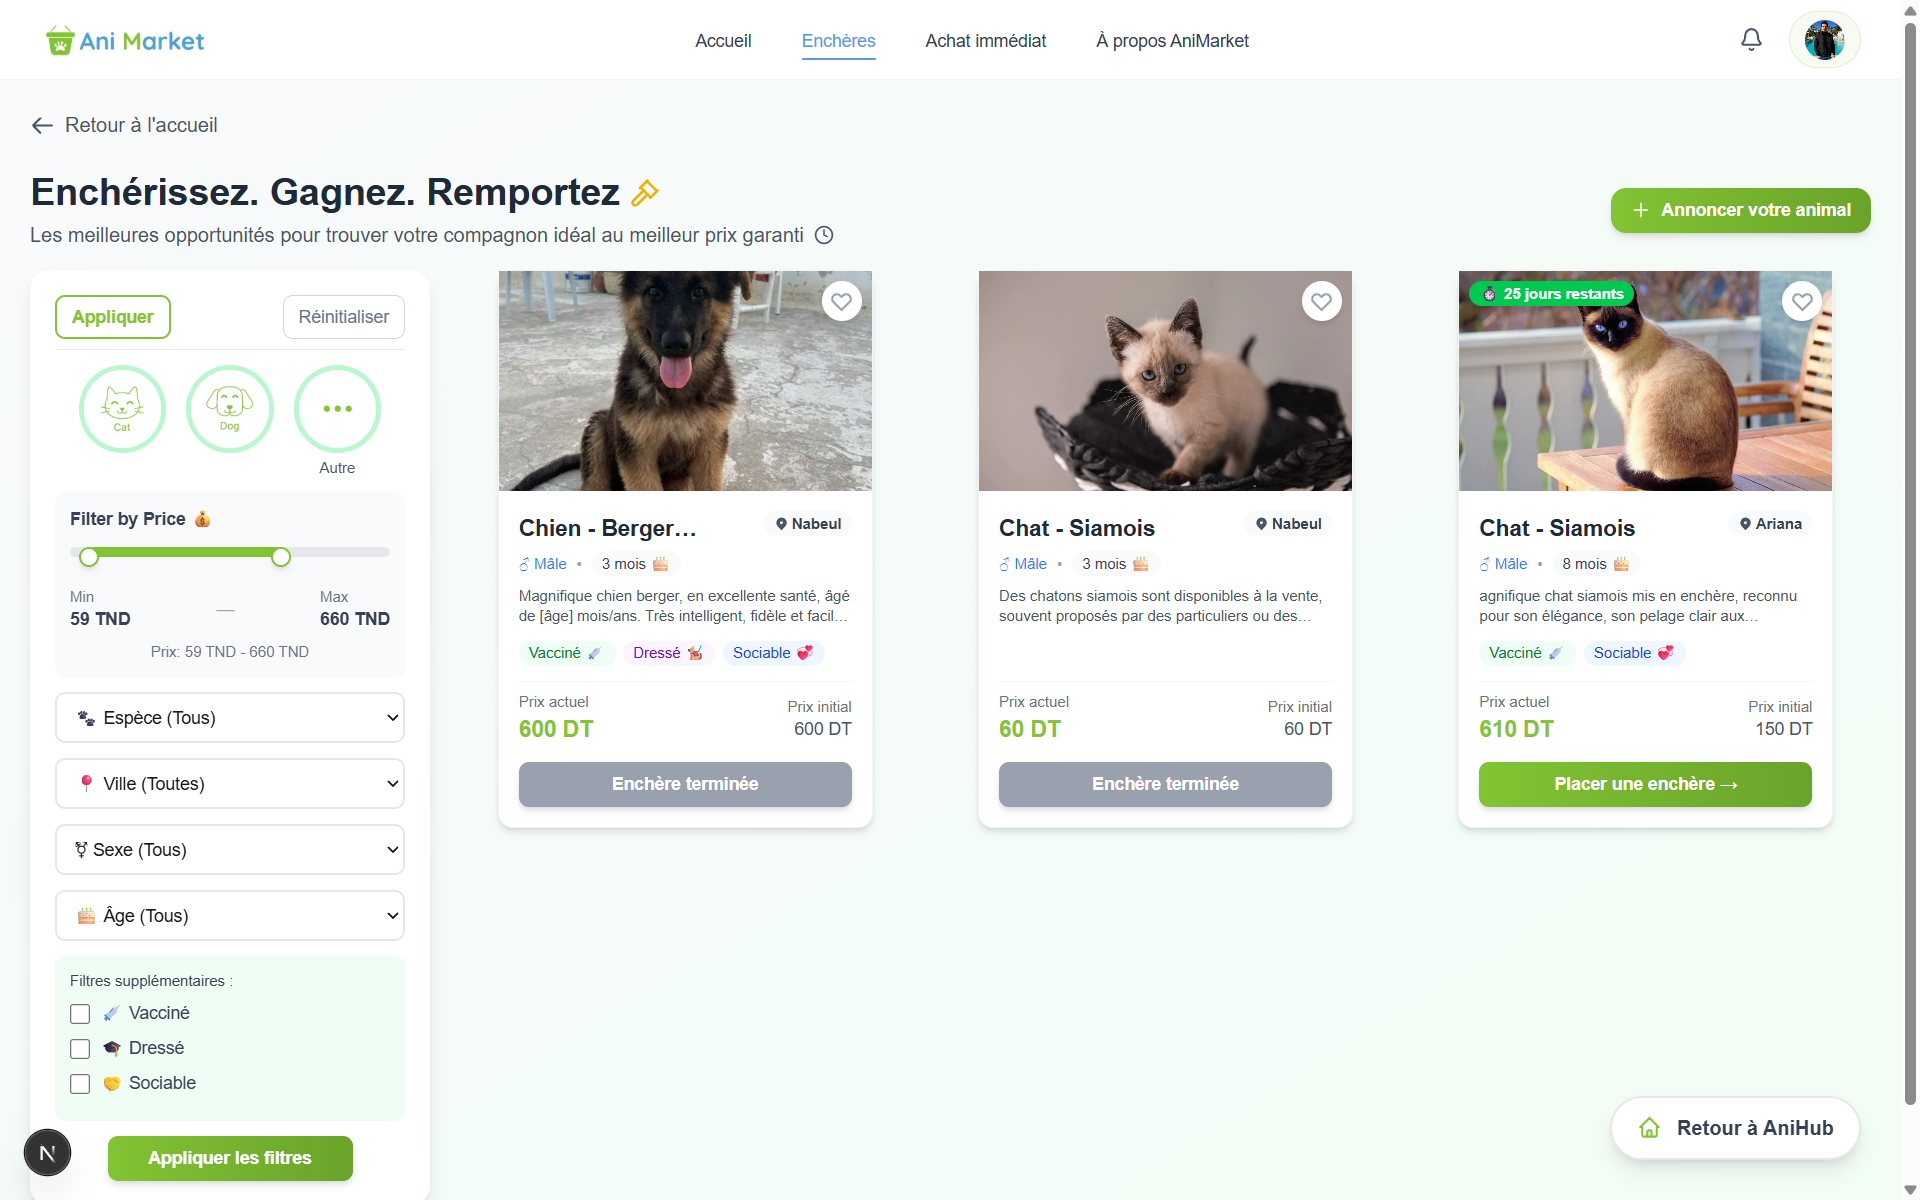
\includegraphics[width=0.77\textwidth]{images/page enchere.png}
    \caption{Interface des enchères}
\end{figure}    
\newpage 
\subsubsection{Interface détails d’une enchère et des offres}

La figure ci-dessous illustre l’interface de détails d’une enchère, présentant les offres proposées, le prix actuel ainsi qu’un formulaire permettant à l’utilisateur de soumettre sa propre offre : 

\begin{figure}[h!]
    \centering
    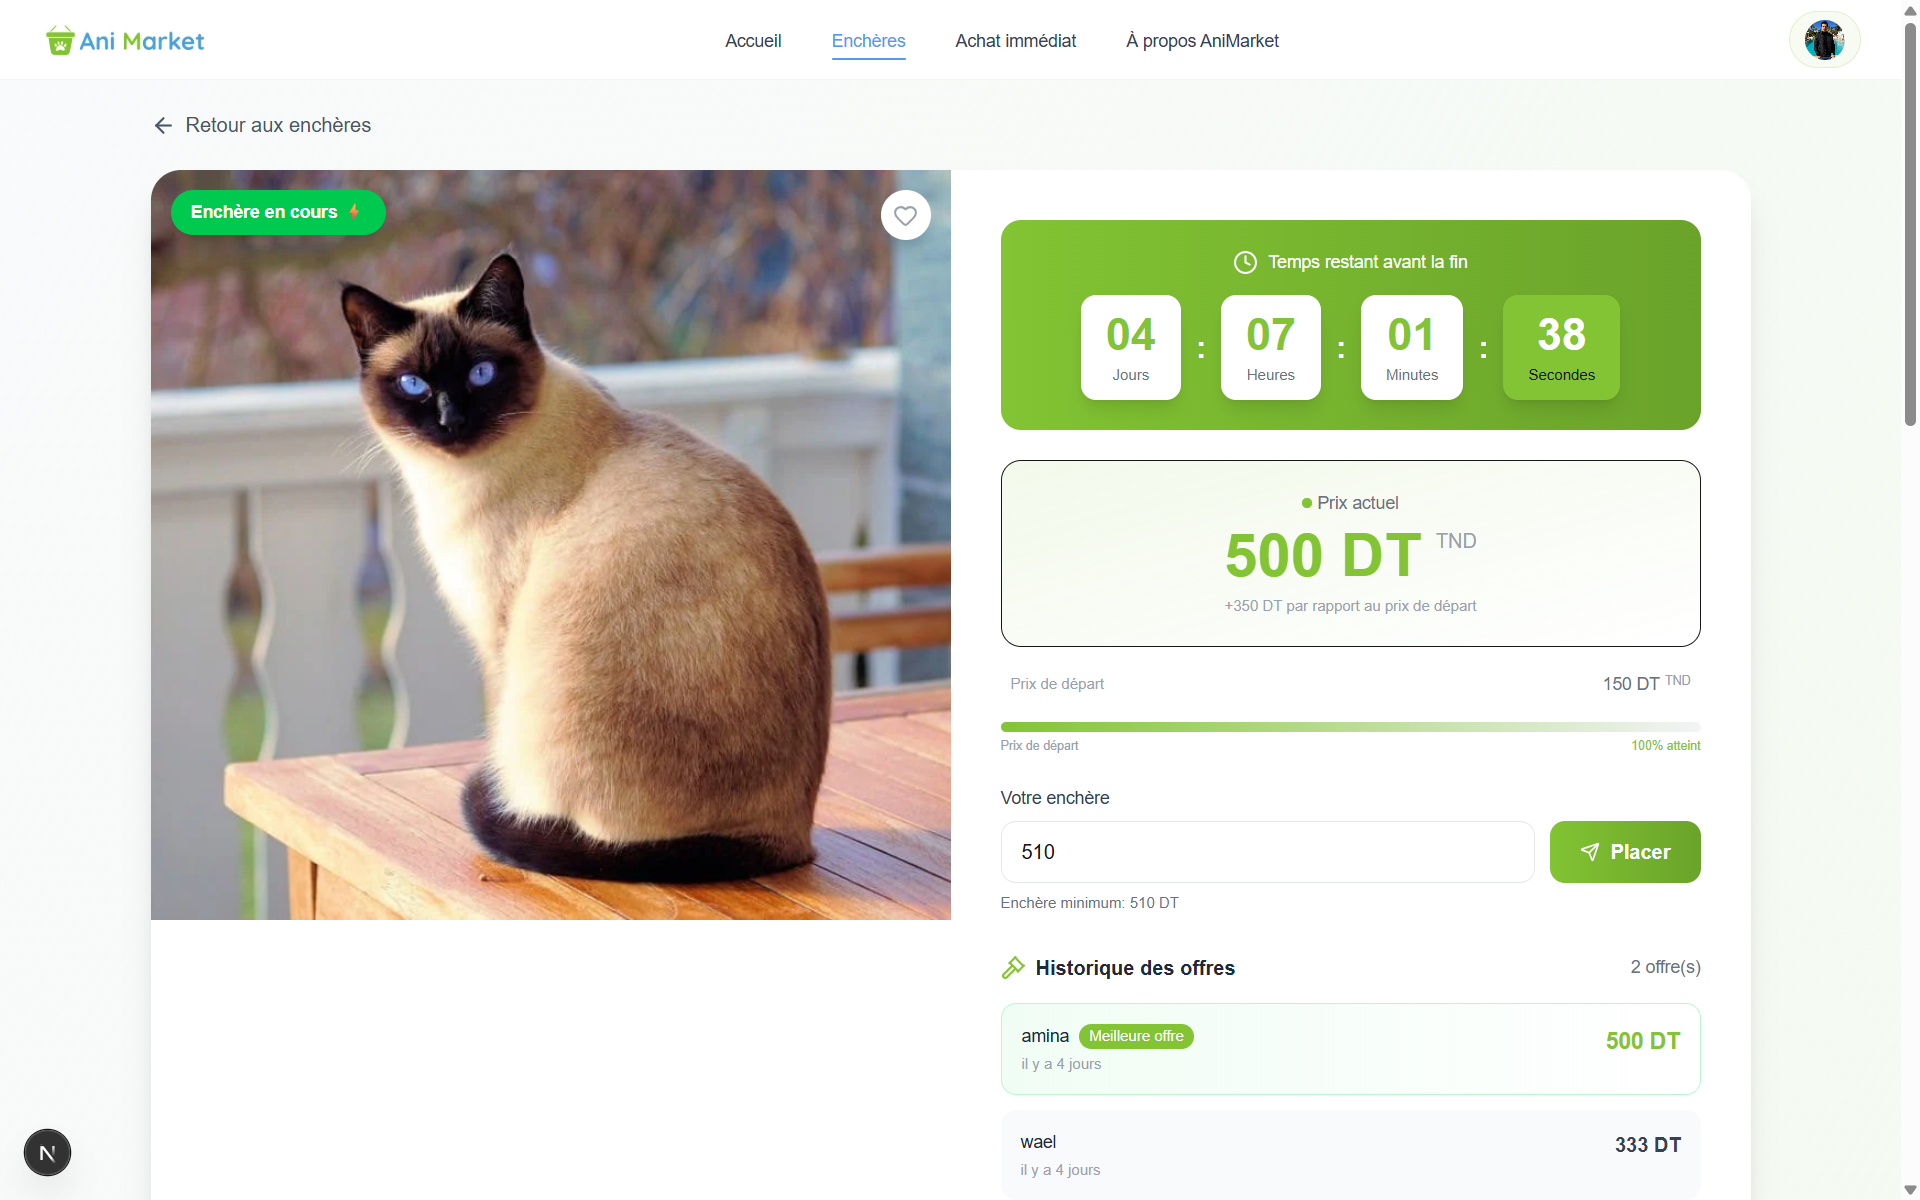
\includegraphics[width=0.75\textwidth]{images/details enchere.png}
    \caption{Interface détails d’une enchère}
\end{figure}    

\subsubsection{Interface des commentaires, avis et enchères similaires}

La figure ci-dessous illustre l’interface des commentaires, avis et enchères similaires : 

\begin{figure}[h!]
    \centering
    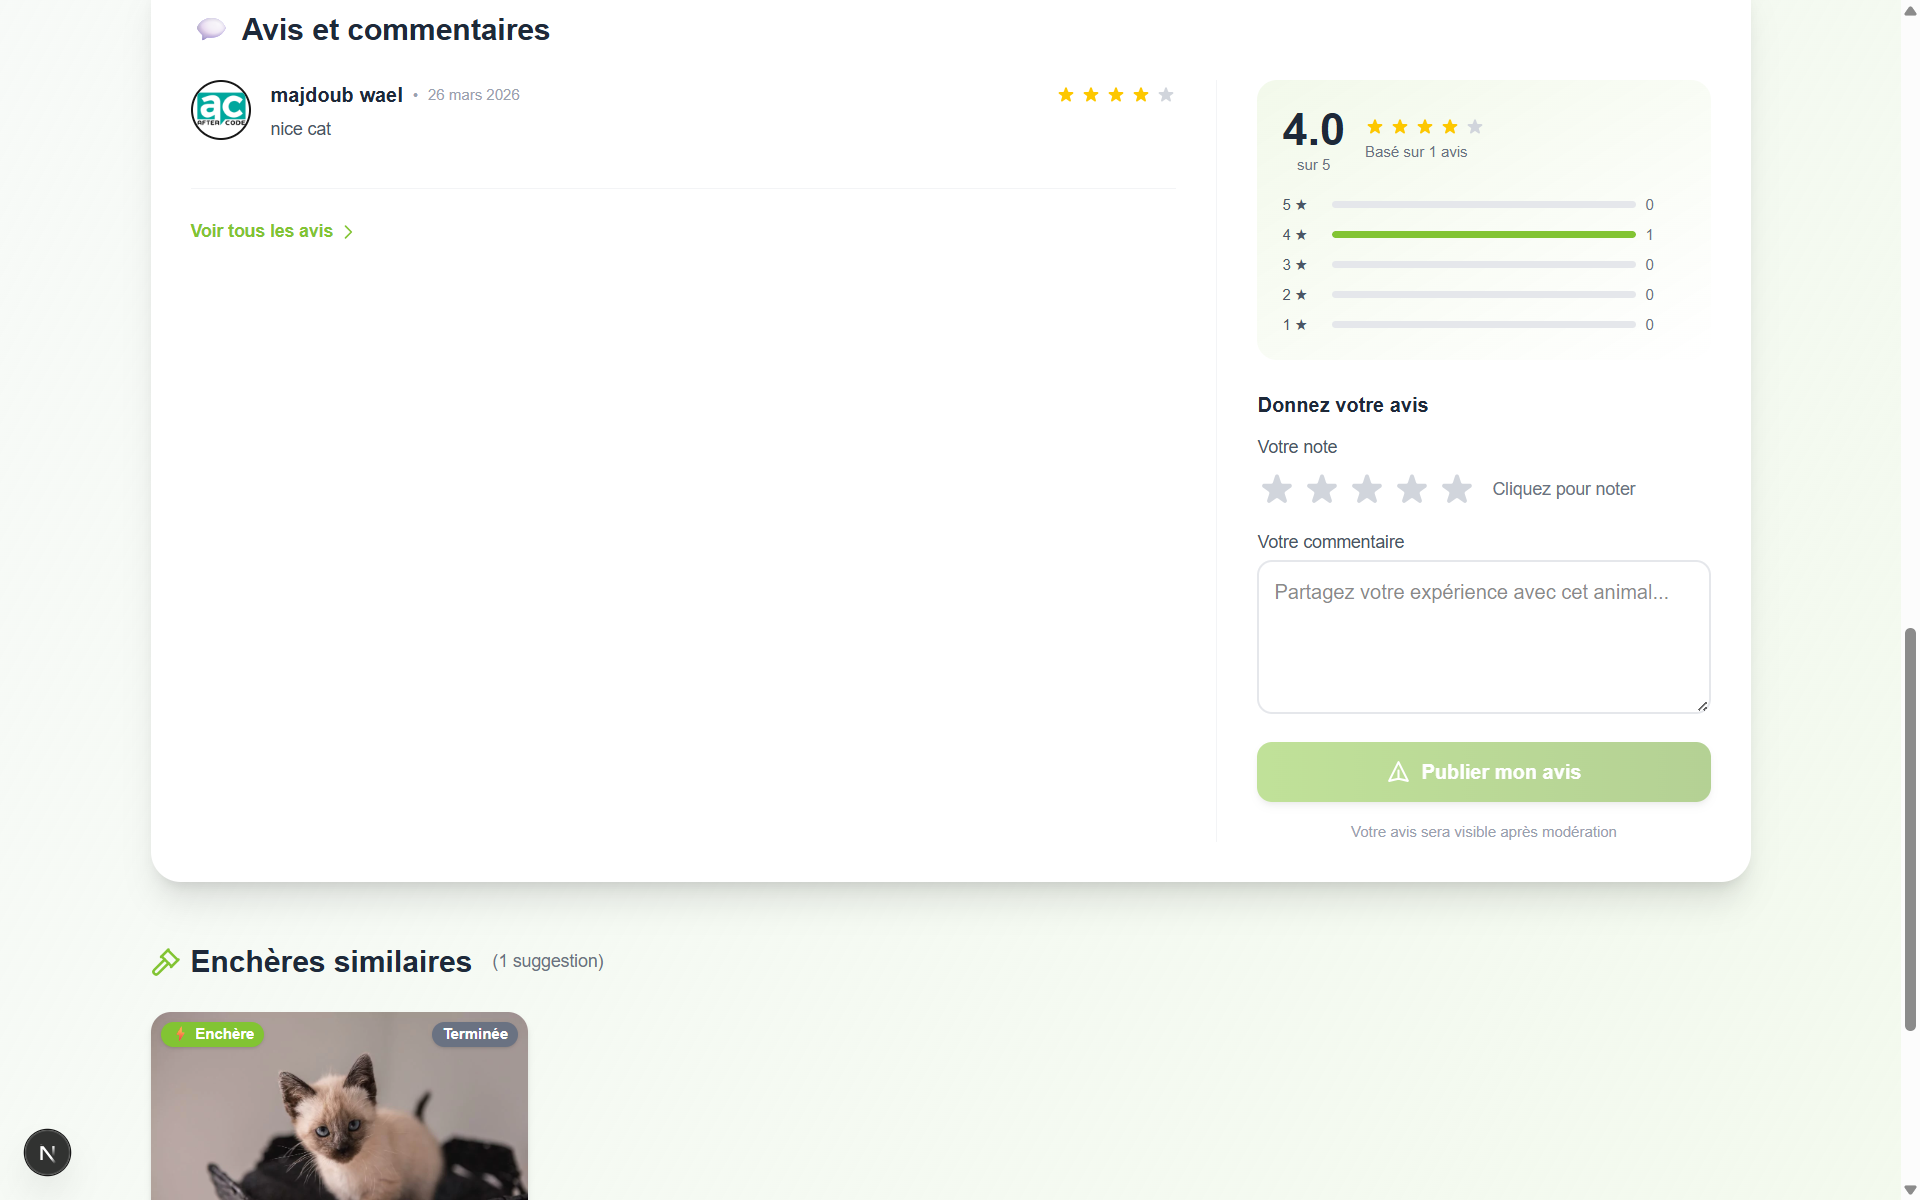
\includegraphics[width=0.72\textwidth]{images/comment section animaux similaires.png}
    \caption{Interface des commentaires, avis et enchères similaires}
\end{figure}    
\newpage  

\subsubsection{Interface notifications reçues}
La figure ci-dessous illustre les notifications reçues par un utilisateur concernant son enchère : 
\begin{figure}[h!]
    \centering
    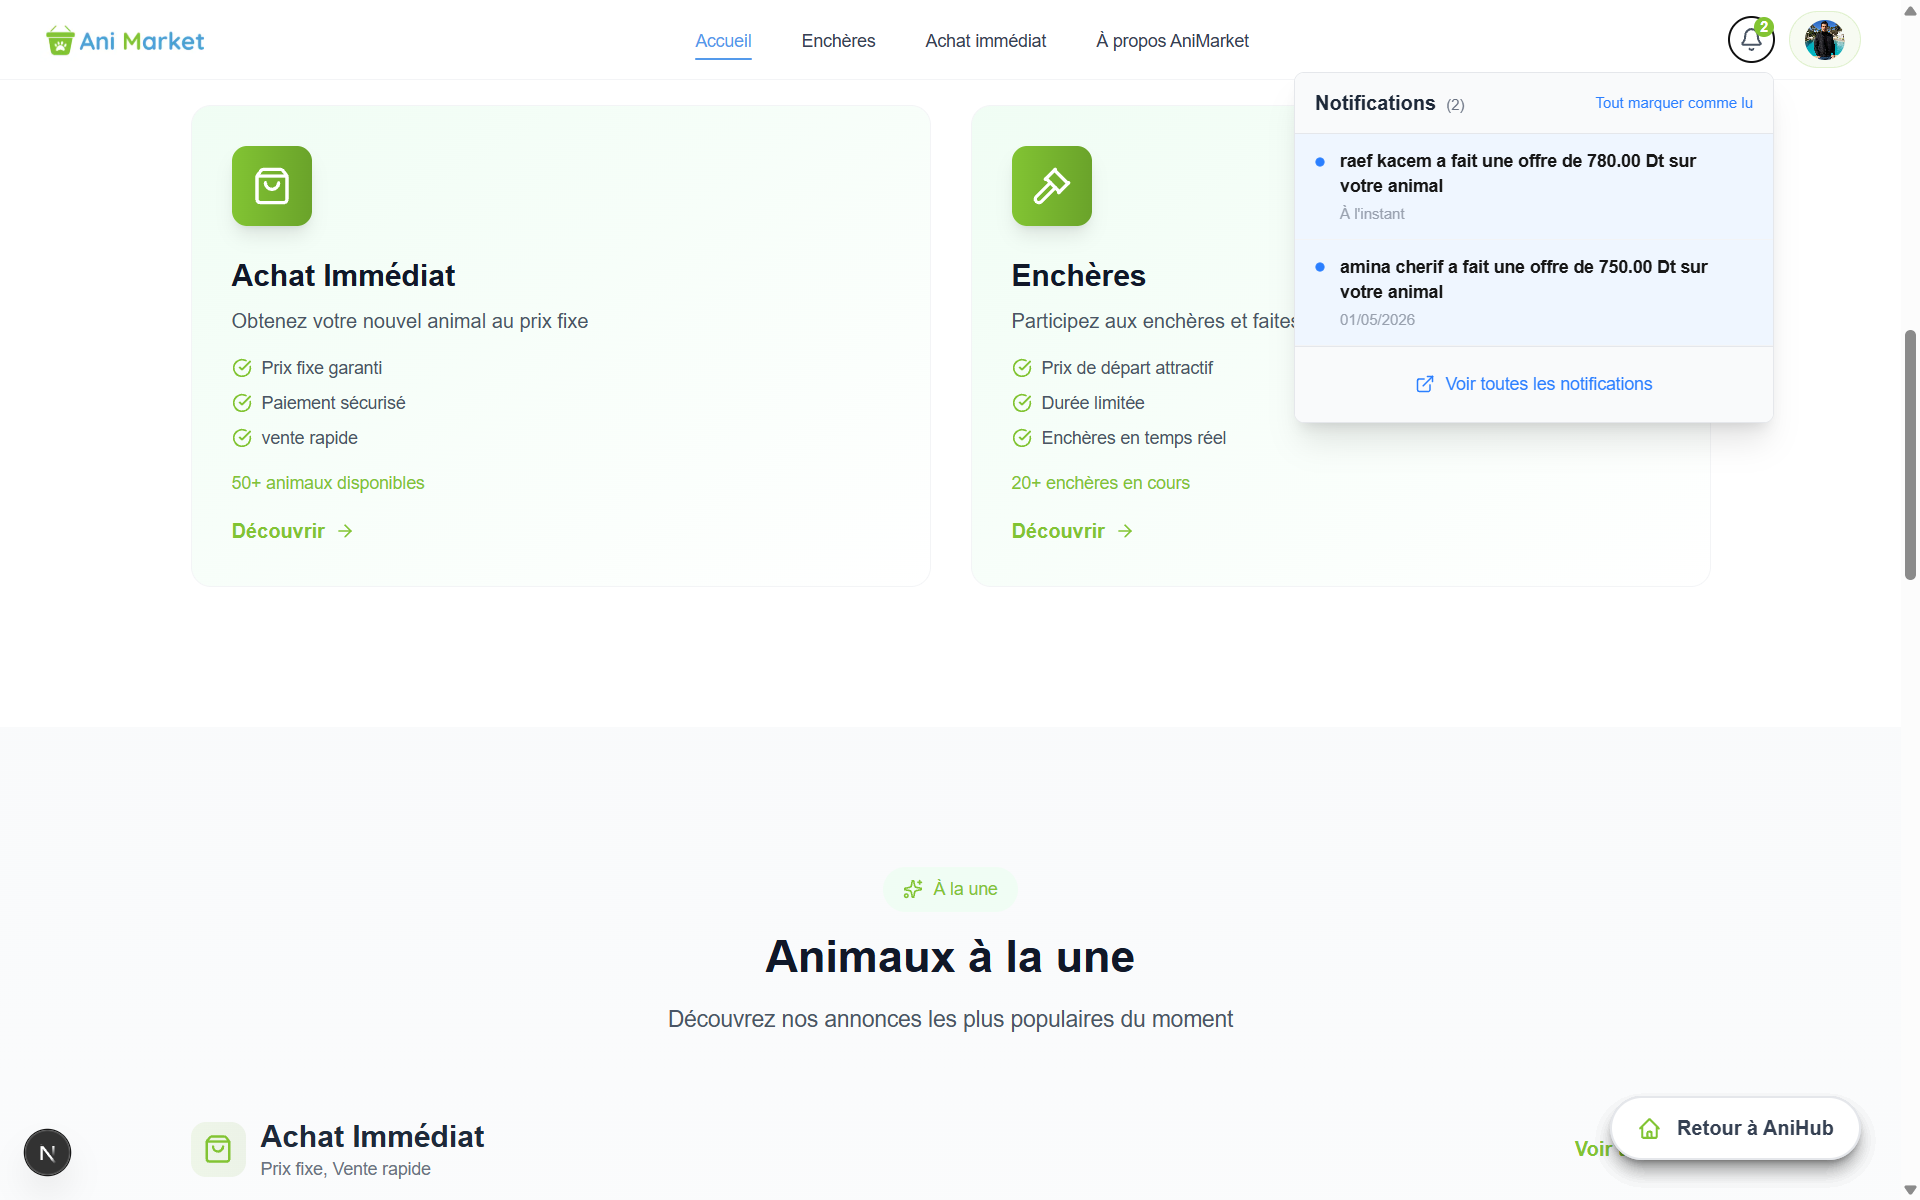
\includegraphics[width=0.77\textwidth]{images/notif animarket.png}
    \caption{Interface notifications reçues}
\end{figure}    

\subsubsection{Interface espace AniMarket} 
La figure ci-dessous présente l’interface AniMarket dédiée au vendeur : 
\begin{figure}[h!]
    \centering
    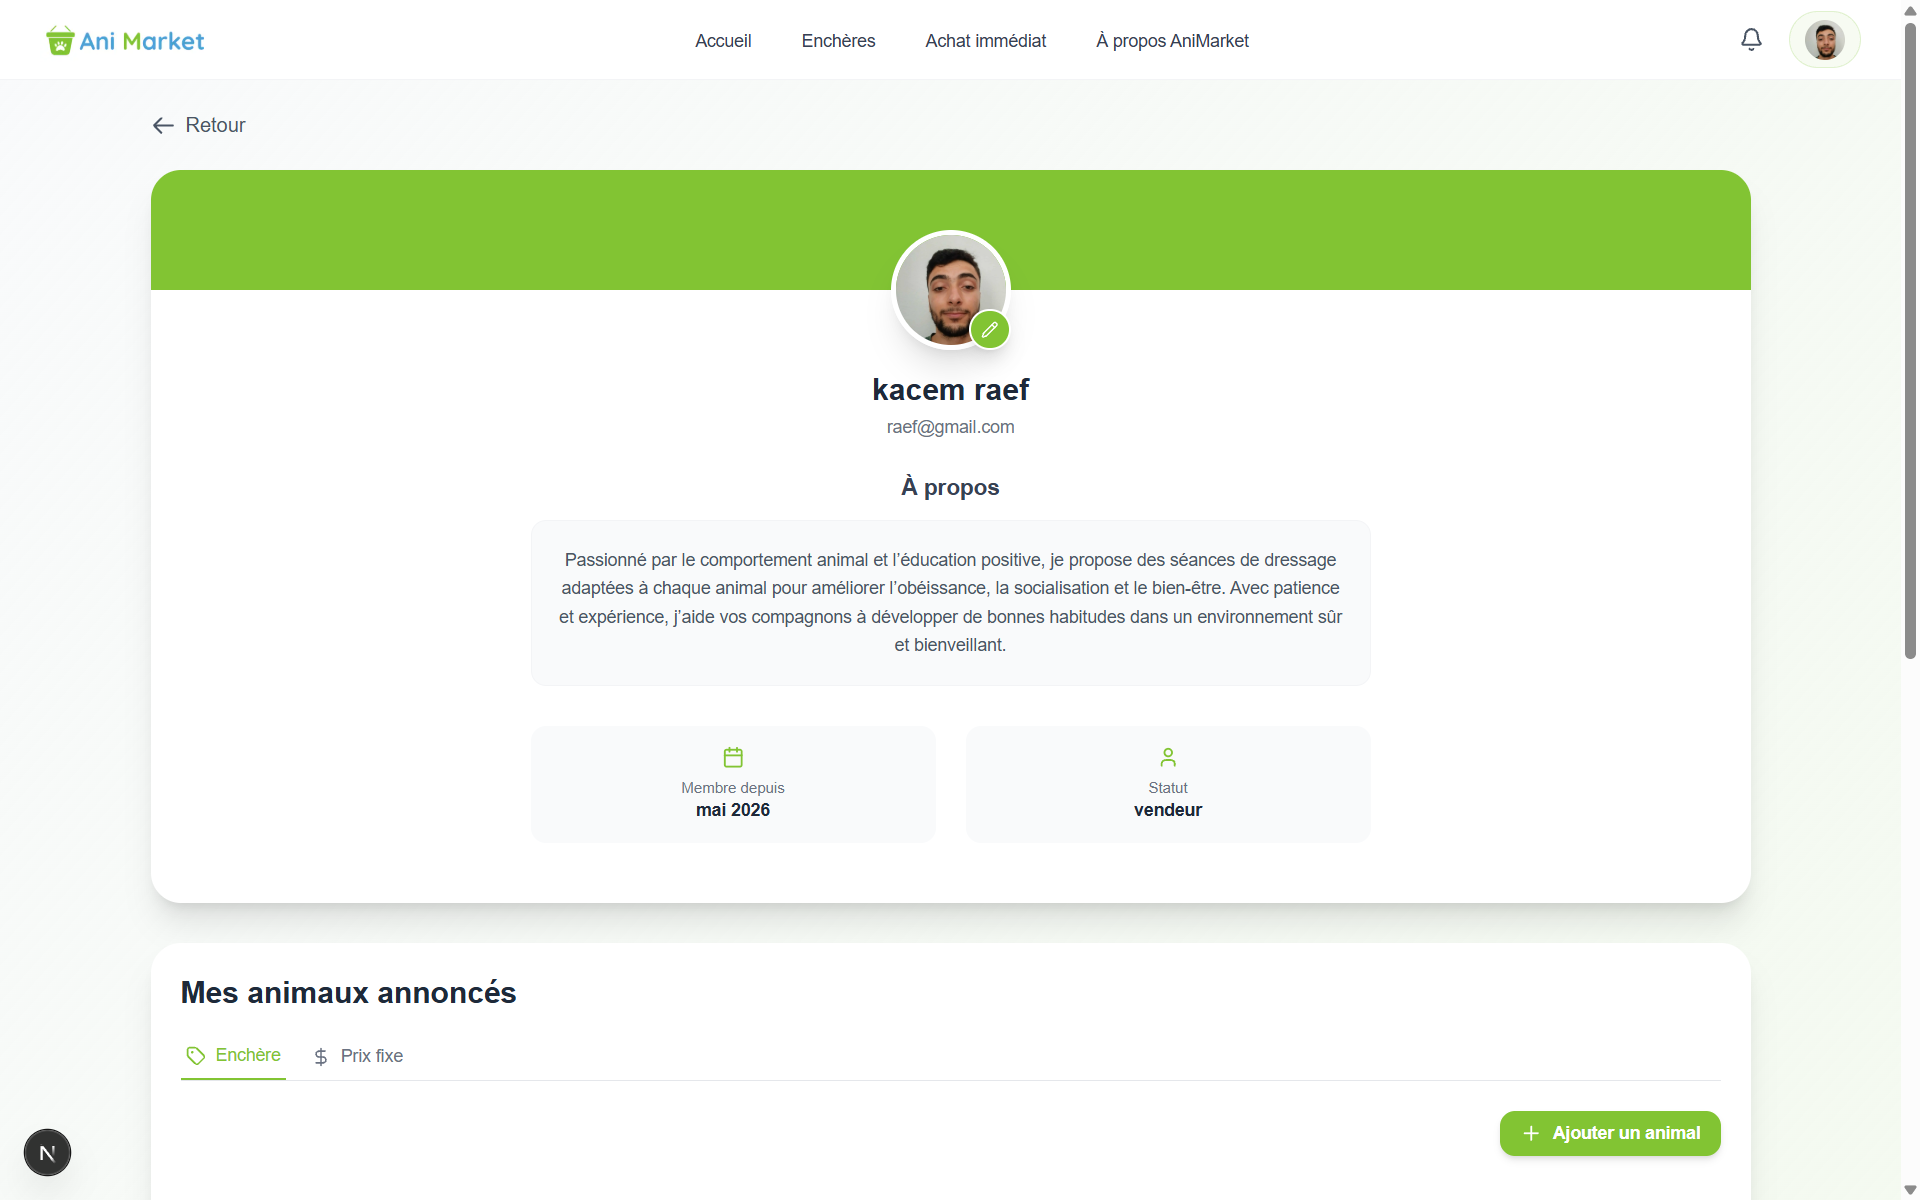
\includegraphics[width=0.77\textwidth]{images/espace animarket profil.png}
    \caption{Interface espace AniMarket}
\end{figure}  

\newpage 
\subsubsection{Interface mes animaux (prix fixe et enchère)} 
La figure ci-dessous illustre l’interface “Mes animaux” avec prix fixe et enchère : 
\begin{figure}[h!]
    \centering
    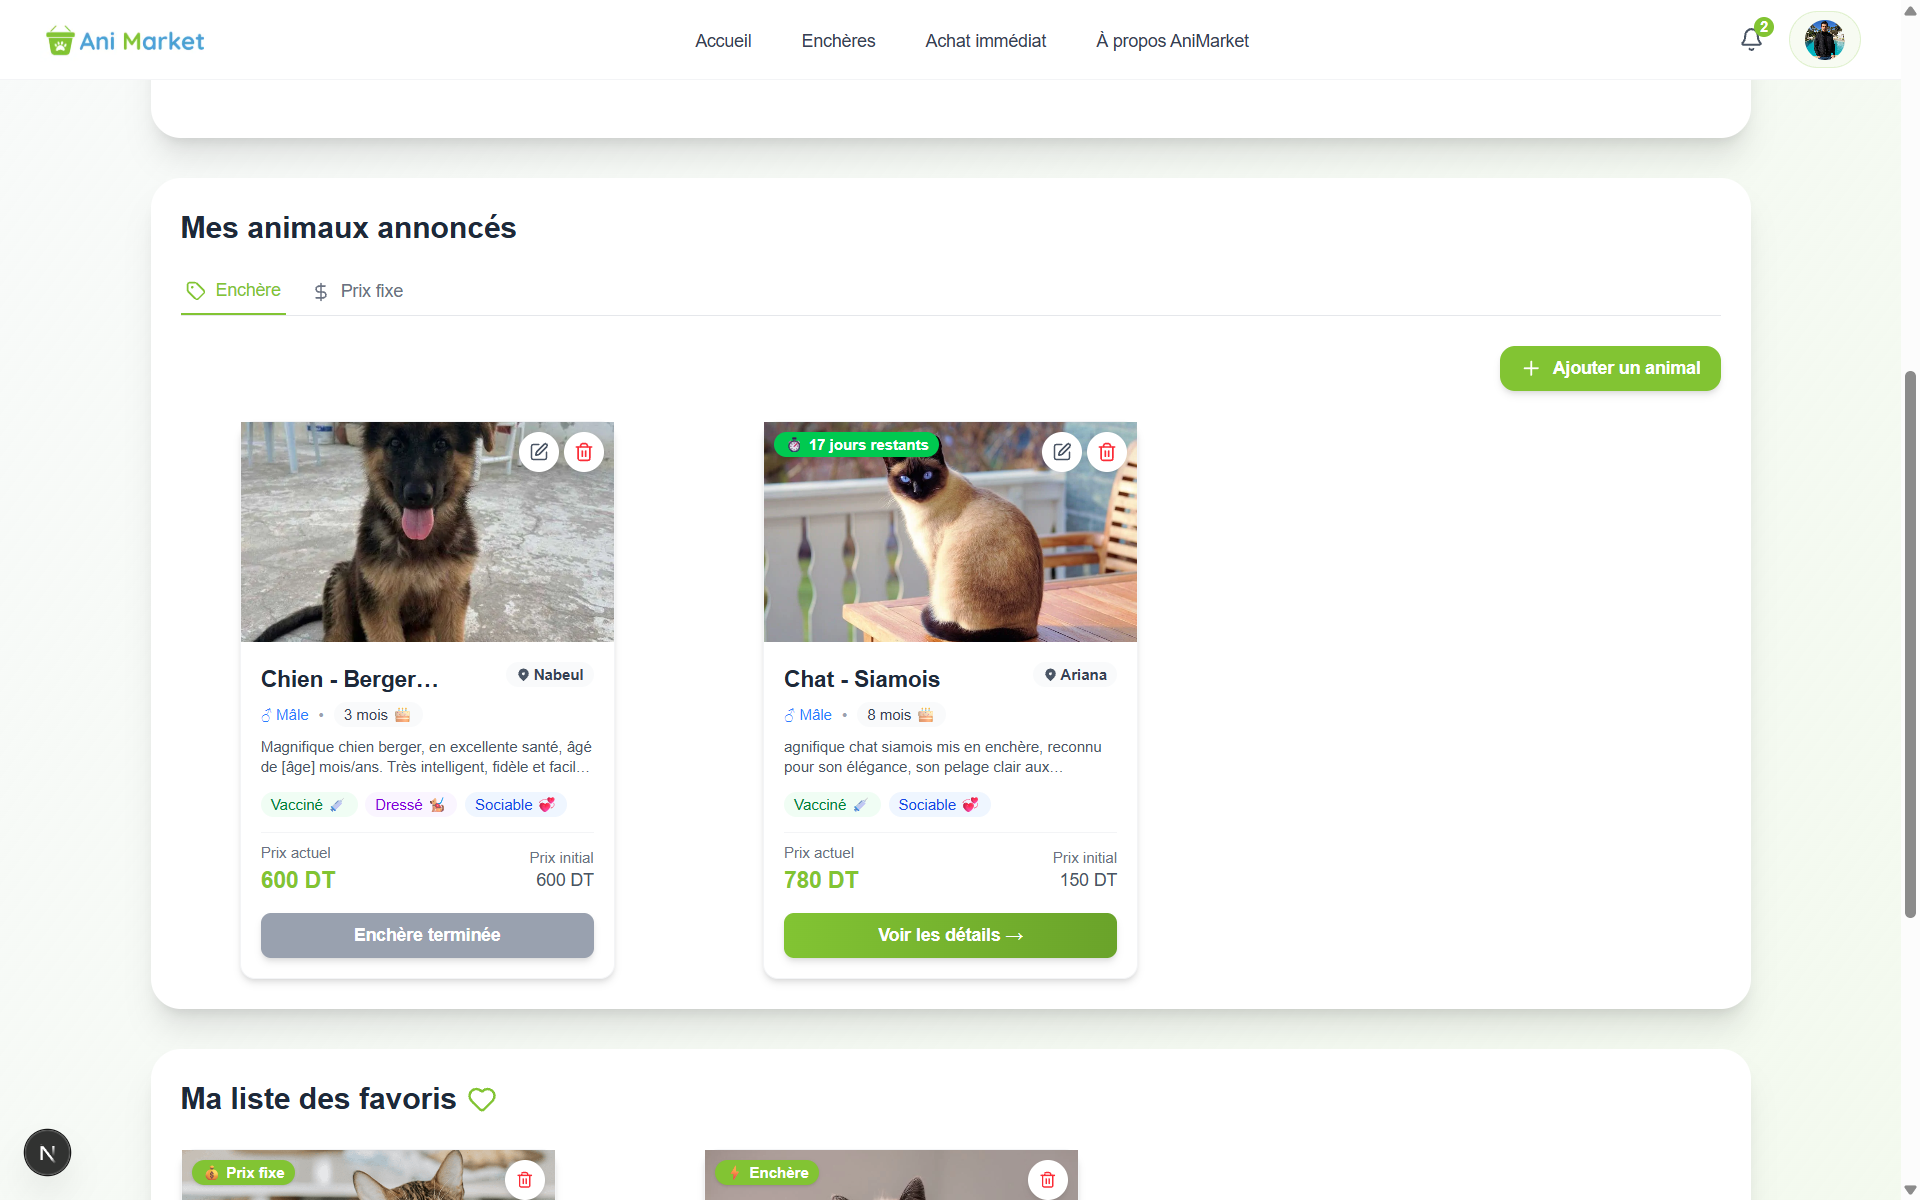
\includegraphics[width=0.77\textwidth]{images/mes animaux animarket.png}
    \caption{Interface mes animaux (prix fixe et enchère)}
\end{figure}  
\subsubsection{Interfaces modiifcation et suppression mes animaux}
Les figures ci-dessous présentent les interfaces de gestion des animaux (modification et suppression)

\begin{figure}[h!]
    \centering
    
    \begin{minipage}{0.48\textwidth}
        \centering
        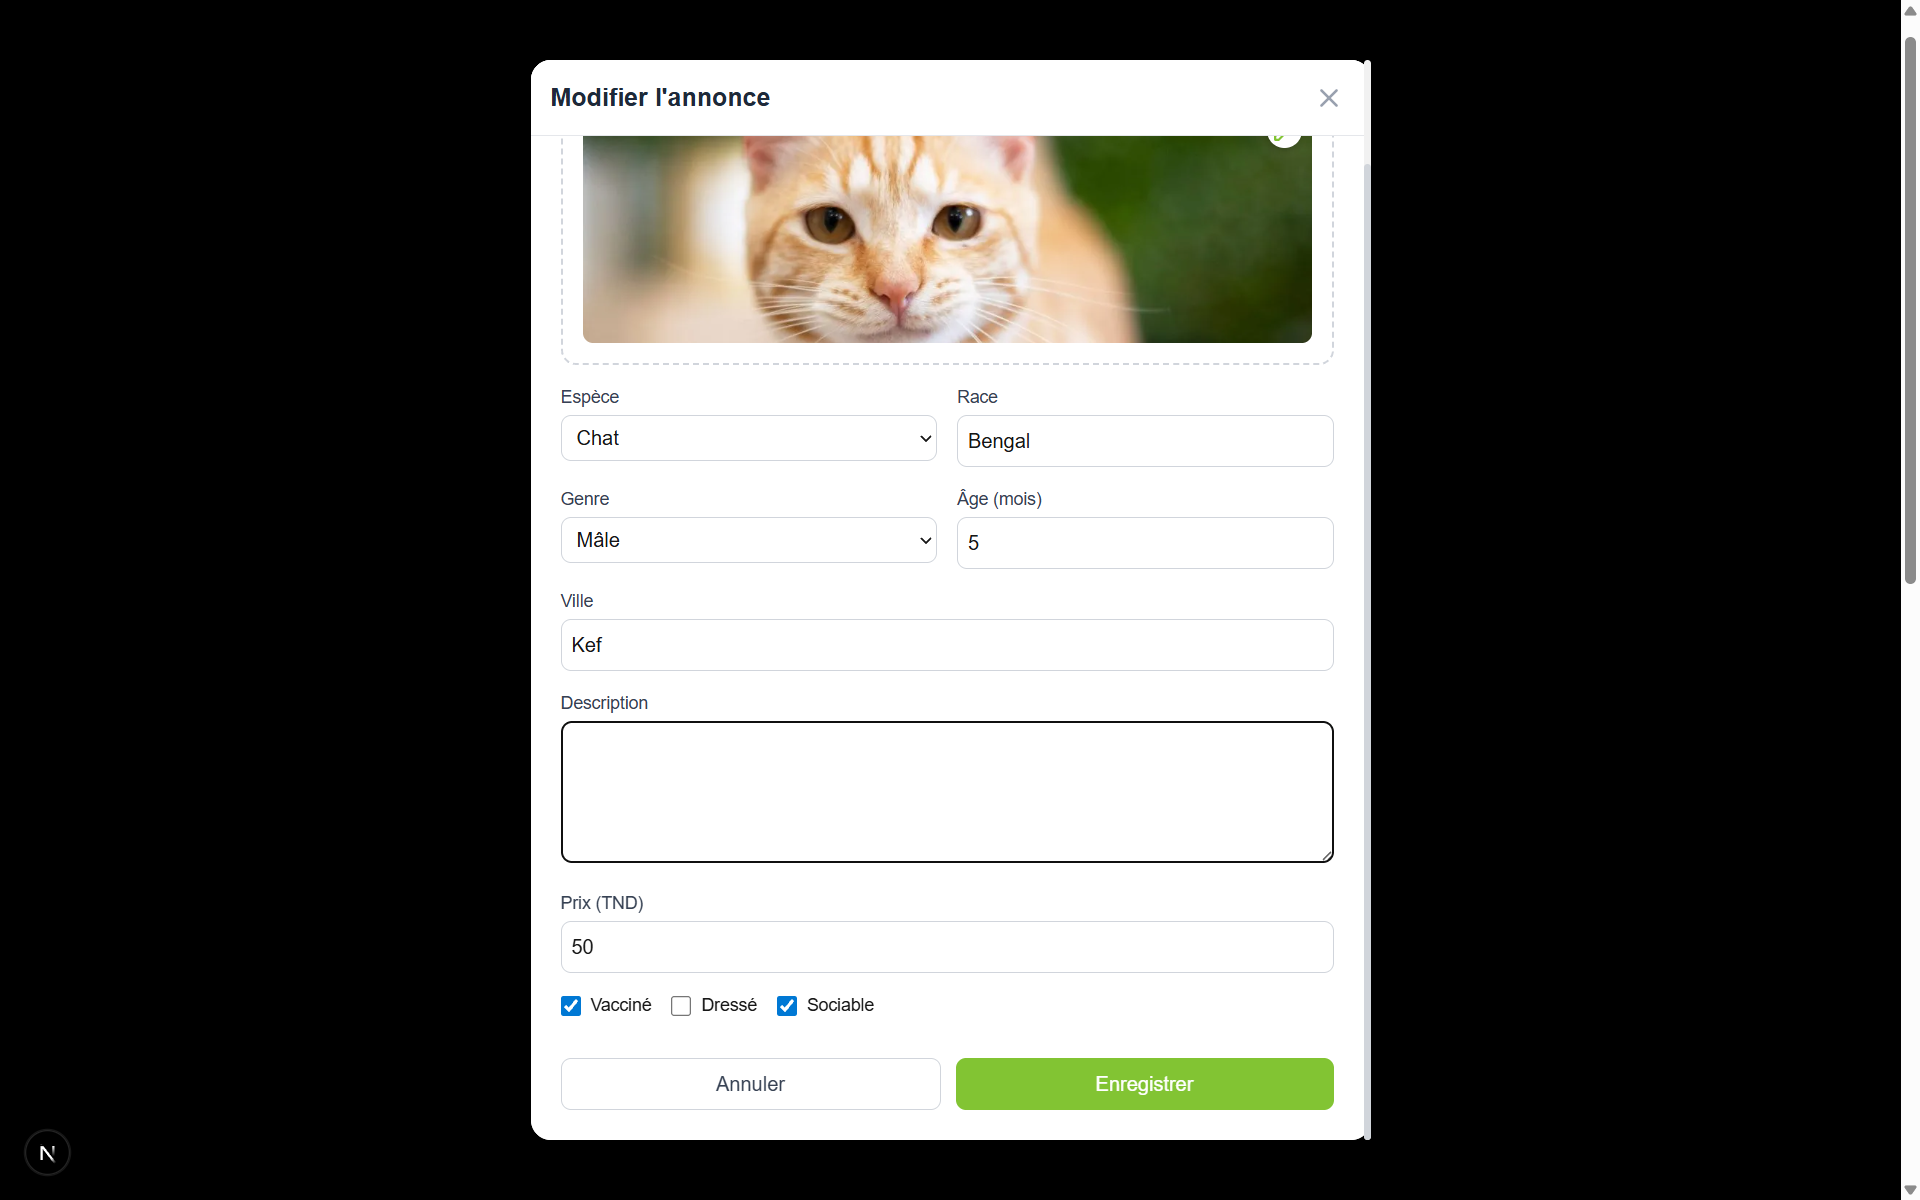
\includegraphics[width=0.85\textwidth]{images/modification animarket.png}
        \caption{Interface modification animal}
    \end{minipage}
    \hfill
    \begin{minipage}{0.48\textwidth}
        \centering
        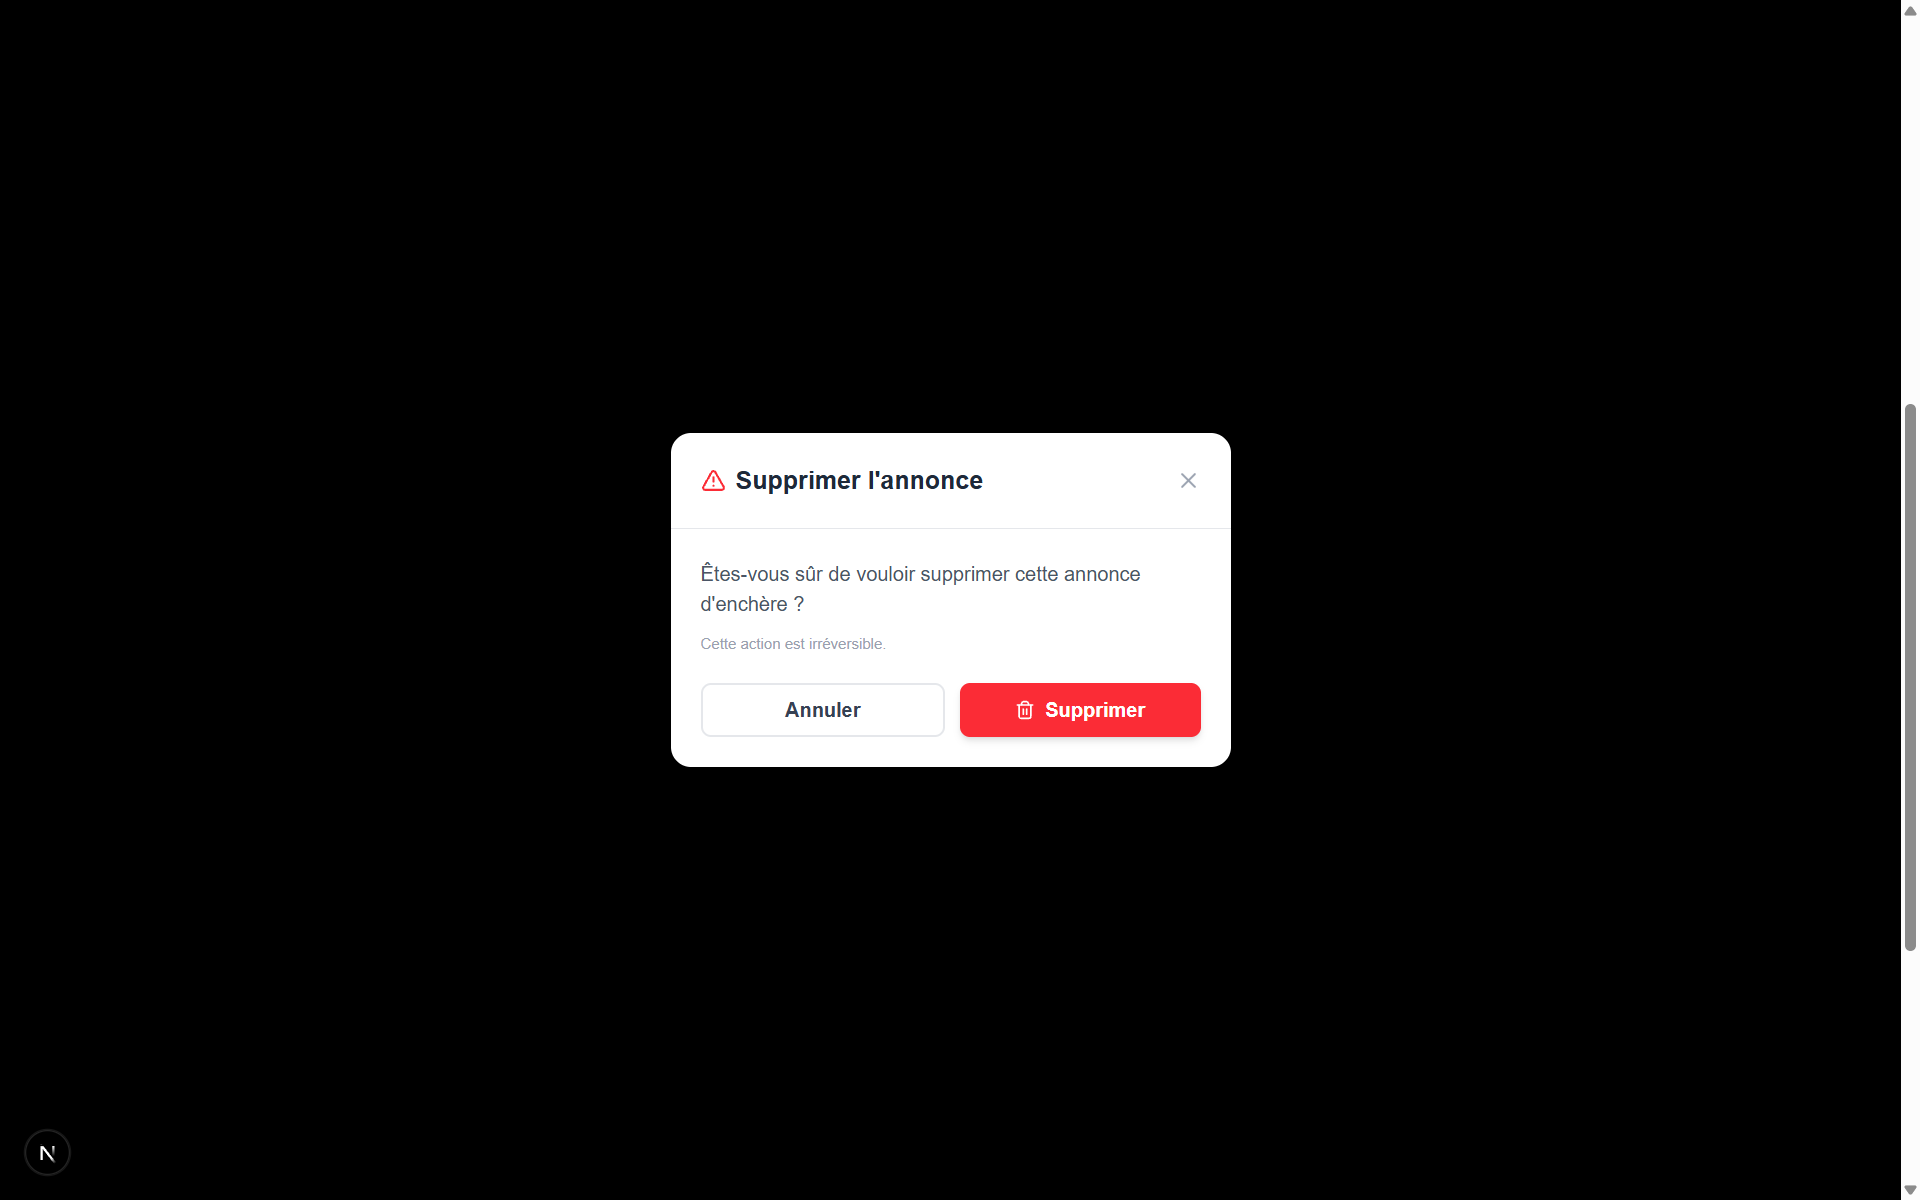
\includegraphics[width=0.85\textwidth]{images/suppression animarket.png}
        \caption{Interface suppression animal}
    \end{minipage}

\end{figure}   













\newpage 
\section{Sprint 5 : AniCare} 
\begin{figure}[H]
    \centering
    
\includegraphics[width=3.8cm]{images/logo anicare.png}
    \caption{Logo du module AniCare}
    \label{fig:logo-anicare}
\end{figure} 
Ce sprint, d’une durée de \textbf{3 semaines}, est dédié au module \textbf{AniCare}, qui permet la gestion et la mise en relation autour des services liés aux animaux. Il offre la possibilité de publier et consulter des services, de gérer les réservations, ainsi que de faciliter la communication entre les utilisateurs et les prestataires. 
\subsection{Sprint backlog}  
Le tableau suivant présente le Sprint Backlog du sprint 5 avec les user stories, les tâches associées et
les efforts estimés : 

\begin{longtable}{|p{2cm}|p{5cm}|p{6cm}|p{2cm}|}
\caption{Sprint Backlog du sprint 5}
\label{tab:sprint-anicare-backlog} \\ 
\hline
\rowcolor{coloranicare}
\textbf{ID} & \textbf{User Story} & \textbf{Tâches} & \textbf{Effort} \\
\hline
\endfirsthead

\hline
\rowcolor{coloranicare}
\textbf{ID} & \textbf{User Story} & \textbf{Tâches} & \textbf{Effort} \\
\hline
\endhead

% ===================== US1 =====================
\multirow{6}{2cm}{US1}
& \multirow{6}{5cm}{En tant qu’utilisateur, je veux consulter la liste des services afin de découvrir les services disponibles et choisir celui qui correspond le mieux à mes besoins}
& Conception UI (Figma) & 0.5 j \\
\cline{3-4}
& & API récupération des services & 1 j \\
\cline{3-4}
& & Filtrage et recherche des services & 0.5 j \\
\cline{3-4}
& & Pagination & 0.5 j \\
\cline{3-4}
& & Commenter et évaluer un service & 0.5 j \\ 
\cline{3-4}
& & ajouter aux favoris & 0.5 j \\
\cline{3-4} 
& & Consulter services similaires & 0.5 j \\
\cline{3-4} 
& & Intégration frontend/backend & 1 j \\
\cline{3-4}
& & Tests & 0.5 j \\
\hline

% ===================== US2 =====================
\multirow{7}{2cm}{US2}
& \multirow{7}{5cm}{En tant qu’utilisateur, je veux gérer mes réservations envoyées (envoyer, suivre, modifier, annuler) afin de gérer efficacement mes demandes}
& Conception UI (Figma) & 0.5 j \\
\cline{3-4}
& & APIs de création, de modification et d’annulation pour mes réservations & 1 j \\
\cline{3-4} 
& & Réserver un service & 0.5 j \\
\cline{3-4}
& & Consulter le statut de mes réservations (acceptée , en attente ou refusée) et modifier ou annuler & 0.5 j \\
\cline{3-4}
& & tests & 0.5 j \\
\hline

% ===================== US3 =====================
\multirow{5}{2cm}{US3}
& \multirow{5}{5cm}{En tant qu’utilisateur, je veux gérer mes notifications afin d’être informé des interactions sur mes activités}
& Analyse besoins notifications & 0.5 j \\
\cline{3-4}
& & Développement MS Notifications & 1 j \\
\cline{3-4}
& & Intégration RabbitMQ avec MS AniCare et le MS notifications & 0.5 j \\
\cline{3-4}
& & Création d’événements (réception, acceptation , refus etc.)& 0.5 j \\
\cline{3-4}
& & Interface notifications frontend & 0.5 j \\
\cline{3-4}
& & Marquer comme lu / non lu & 0.5 j \\
\hline

% ===================== US4 =====================
\multirow{5}{2cm}{US4}
& \multirow{5}{5cm}{En tant qu’utilisateur, je veux discuter avec l'autre partie (utilisateur ou prestataire)}
& Analyse & 0.5 j \\
\cline{3-4}
& & Intégration bouton WhatsApp & 0.5 j \\
\cline{3-4}
& & Génération lien wa.me & 0.5 j \\
\cline{3-4}
& & Tests & 0.5 j \\
\hline

% ===================== US5 =====================
\multirow{7}{2cm}{US5}
& \multirow{7}{5cm}{En tant que prestataire de service, je veux gérer mon propre service (publier, mettre à jour, supprimer) afin de présenter mes services de manière claire}
& Conception UI (Figma) & 0.5 j \\
\cline{3-4}
& & APIs création , modification et suppression service & 1 j \\
\cline{3-4} 
& & Intégration avec microservice Auth (JWT, sécurité API) & 0.5 j \\
\cline{3-4}
& & Upload d’images et de documents justificatifs sur Cloudinary& 0.5 j \\
\cline{3-4}
& & Intégration frontend/backend & 0.5 j \\ 
\cline{3-4} 
& & Tests & 0.5 j \\
\hline

% ===================== US6 =====================
\multirow{6}{2cm}{US6}
& \multirow{6}{5cm}{En tant que prestataire de service, je veux gérer mes réservations reçues afin de répondre aux demandes des clients et organiser efficacement mes prestations}
& Conception UI (Figma) & 0.5 j \\
\cline{3-4} 
& & APIs de récupération et de modification du statut (confirmée ou refusée) des réservations reçues & 1 j \\
\cline{3-4} 
& & Changement du statut de la réservation (accepter ou refuser) depuis le frontend & 0.5 j \\
\cline{3-4}
& & Développement du calendrier du prestataire & 1 j \\
\cline{3-4}
& & Affichage des réservations des utilisateurs dans le calendrier du prestatire & 0.5 j \\
\cline{3-4}
& & Tests & 0.5 j \\
\hline

\end{longtable}
\newpage 
\subsection{Diagramme des cas d’utilisation du sprint 5} 

Dans cette section, nous présentons le diagramme des cas d’utilisation du sprint 5, dédié au module \textbf{AniCare}. Ce diagramme illustre les principales interactions entre l’utilisateur et le prestataire de service avec le système . 

La figure ci-dessous représente le diagramme des cas d’utilisation correspondant : 


\begin{figure}[H]
    \centering
  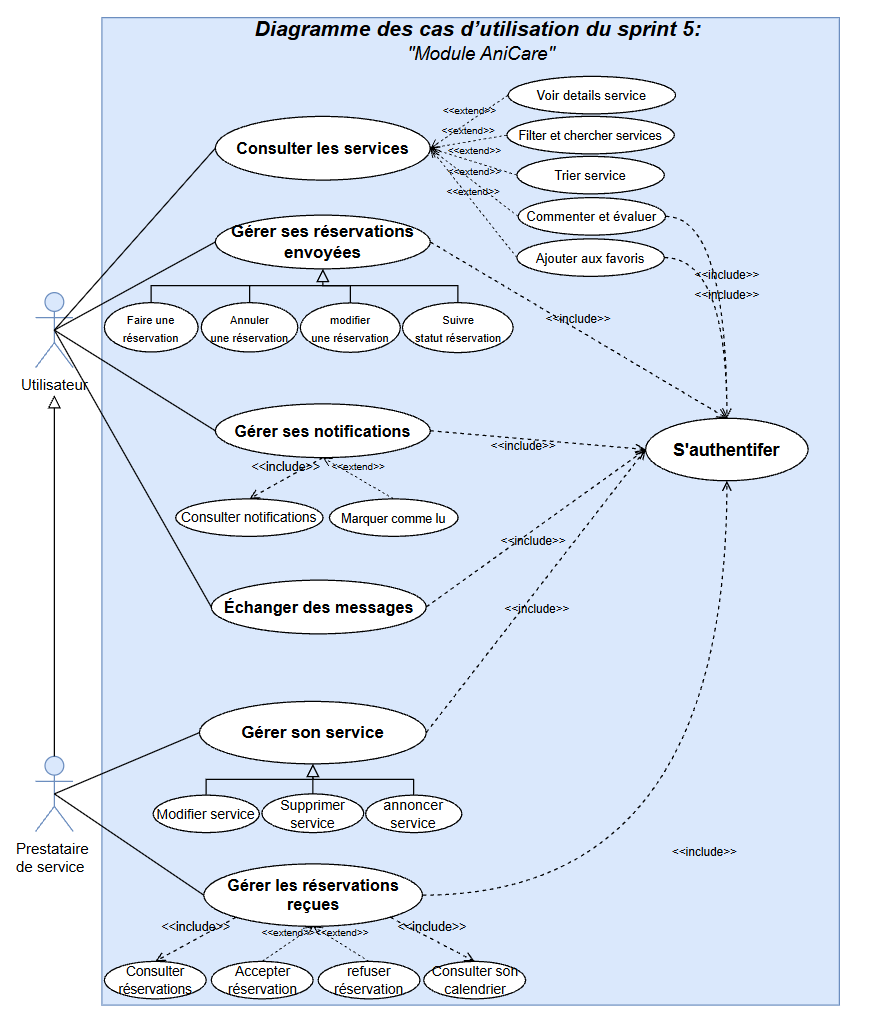
\includegraphics[width=1.05\linewidth, height=19.5cm, keepaspectratio]{images/use case anicare.png}
    \caption{Diagramme des cas d’utilisation du sprint 5}
    \label{fig:usecase-sprint5}
\end{figure} 

\newpage 
\subsection{Descriptions textuelles des cas d’utilisation du sprint 5}   
Cette section présente les cas d’utilisation du sprint 5 du module AniCare : 
\subsubsection{ Description textuelle du cas d’utilisation «Consulter les services» } 
Le tableau ci-dessous présente le cas d’utilisation « Consulter les services » :  

\begin{longtable}{|c|p{11cm}|}
\caption{Description textuelle du cas d’utilisation "Consulter les services"}
\label{tab:consulter_services} \\
\hline
\cellcolor{coloranicare} \textbf{Nom du cas d'utilisation } & Consulter les services \\
\hline
\cellcolor{coloranicare} \textbf{Acteurs} & Utilisateur \\
\hline
\cellcolor{coloranicare} \textbf{Description } & Tout utilisateur du système peut consulter les services du module "AniCare" proposés par les prestataires de service. \\
\hline
\cellcolor{coloranicare} \textbf{Pré-condition } & Accès libre à la page d’accueil sans authentification. \\
\hline
\cellcolor{coloranicare} \textbf{Post-condition } & L’utilisateur a consulté les services et peut interagir avec un service. \\
\hline

\cellcolor{coloranicare} \textbf{Scénario nominal } & 
\begin{enumerate}
\item L’utilisateur accède à la page d’accueil d’AniHub.
\item L’utilisateur choisit le module AniCare.
\item Le système redirige l’utilisateur vers AniCare.
\item L’utilisateur accède à la section « Services ».
\item Le système affiche la liste des services disponibles.
\item L’utilisateur peut filtrer les services selon des critères (type service , ville , etc.).
\item Le système affiche la liste des services filtrés.
\item L’utilisateur clique sur un service.
\item Le système affiche les détails du service.
\item L’utilisateur authentifié ajoute un service à sa wishlist.
\item Le système ajoute le service à la wishlist.
\item L’utilisateur authentifié peut saisir un commentaire, attribuer une note et cliquer sur « Publier ».
\item Le système vérifie, enregistre le commentaire et la note et met à jour la liste des avis affichés.
\end{enumerate} \\

\hline
\cellcolor{coloranicare} \textbf{Scénario alternatif :} &
Message d’erreur affiché si l’utilisateur n’est pas authentifié lors de l’ajout à la wishlist ou de la publication d’un commentaire. \\
\hline

\end{longtable}
 \newpage 
 \subsection{Description textuelle du cas d’utilisation «Gérer ses réservations envoyées»} 
\begin{longtable}{|c|p{11cm}|}
\caption{Description textuelle du cas d’utilisation "Gérer ses réservations envoyées"}
\label{tab:gerer_reservations_envoyees} \\
\hline
\cellcolor{coloranicare} \textbf{Nom du cas d'utilisation } & Gérer ses réservations envoyées \\
\hline
\cellcolor{coloranicare} \textbf{Acteurs} & Utilisateur \\
\hline
\cellcolor{coloranicare} \textbf{Description } & 
L’utilisateur peut envoyer une réservation, consulter  statut, modifier ou annuler une réservation existante. \\
\hline

\cellcolor{coloranicare} \textbf{Pré-condition } & L’utilisateur doit être authentifié. \\
\hline

\cellcolor{coloranicare} \textbf{Post-condition } & Les réservations envoyées sont traitées avec succès.\\
\hline

\cellcolor{coloranicare} \textbf{Scénario nominal } &
\begin{enumerate}
\item L’utilisateur accède à « AniCare » et choisit la section « Services ».
\item Le système affiche la liste des services disponibles.
\item L’utilisateur clique sur un service.
\item Le système affiche les détails du service.

\item Selon l’action de l’utilisateur :

\begin{itemize}

\item \textbf{Cas 1 : Envoi d’une réservation}
\begin{enumerate}
\item L’utilisateur choisit un créneau et envoie une réservation.
\item Le système enregistre la réservation.
\item Le système notifie le prestataire.
\end{enumerate}

\end{itemize}

\item L’utilisateur accède à « Mon espace AniCare ».
\item Le système affiche la liste des réservations envoyées.
\item L’utilisateur sélectionne une réservation.

\begin{itemize}

\item \textbf{Cas 2 : Modification d’une réservation}
\begin{enumerate}
\item L’utilisateur modifie les informations et valide.
\item Le système met à jour la réservation.
\end{enumerate}

\item \textbf{Cas 3 : Annulation d’une réservation}
\begin{enumerate}
\item L’utilisateur clique sur « Annuler ».
\item Le système supprime la réservation.
\end{enumerate}

\end{itemize}

\end{enumerate} \\
\hline

\cellcolor{coloranicare} \textbf{Scénario alternatif :} &
\begin{itemize}
\item Message d’erreur si le créneau sélectionné n’est plus disponible.
\item Message d’erreur si la réservation ne peut pas être modifiée ou annulée.
\end{itemize} \\
\hline

\end{longtable} 
\newpage 
\subsection{Description textuelle du cas d’utilisation «Gérer ses réservations reçues»} 
\begin{longtable}{|c|p{11cm}|}
\caption{Description textuelle du cas d’utilisation "Gérer ses réservations reçues"}
\label{tab:gerer_reservations_recues} \\
\hline
\cellcolor{coloranicare} \textbf{Nom du cas d'utilisation } & Gérer ses réservations reçues \\
\hline
\cellcolor{coloranicare} \textbf{Acteurs} & Prestataire de service \\
\hline
\cellcolor{coloranicare} \textbf{Description } & 
Le prestataire de service peut consulter son calendrier, accepter ou refuser les réservations reçues. \\
\hline

\cellcolor{coloranicare} \textbf{Pré-condition } & Le prestataire doit être authentifié. \\
\hline

\cellcolor{coloranicare} \textbf{Post-condition } & Les réservations sont mises à jour avec succès. \\
\hline

\cellcolor{coloranicare} \textbf{Scénario nominal } &
\begin{enumerate}
\item Le prestataire accède à « AniCare ».
\item Le prestataire accède à son espace AniCare.
\item Le système affiche les réservations reçues.
\item Le prestataire consulte son calendrier.
\item Le système affiche les réservations dans le calendrier.

\item Selon l’action du prestataire :

\begin{itemize}

\item \textbf{Cas 1 : Acceptation d’une réservation}
\begin{enumerate}
\item Le prestataire sélectionne une réservation.
\item Le prestataire clique sur « Accepter ».
\item Le système met à jour le statut de la réservation.
\item Le système notifie l’utilisateur.
\end{enumerate}

\item \textbf{Cas 2 : Refus d’une réservation}
\begin{enumerate}
\item Le prestataire sélectionne une réservation.
\item Le prestataire clique sur « Refuser ».
\item Le système met à jour le statut de la réservation.
\item Le système notifie l’utilisateur.
\end{enumerate}

\end{itemize}

\end{enumerate} \\
\hline

\cellcolor{coloranicare} \textbf{Scénario alternatif :} &
\begin{itemize}
\item Si aucune réservation n’est reçue, le système affiche un message indiquant qu’aucune réservation n’est disponible.
\item Si le créneau demandé est déjà occupé, le système empêche l’acceptation de la réservation.
\end{itemize} \\
\hline

\end{longtable} 
\newpage 
\subsubsection{Description textuelle du cas d’utilisation « Gérer mon service »}
\begin{longtable}{|c|p{11cm}|}
\caption{Description textuelle du cas d'utilisation "Gérer mon service"}
\label{tab:gerer_service} \\
\hline
\cellcolor{coloranicare}\textbf{Nom du cas d'utilisation } & Gérer mon service \\
\hline
\cellcolor{coloranicare}\textbf{Acteurs} & Prestataire de service \\
\hline
\cellcolor{coloranicare}\textbf{Description } & Le prestataire de service peut publier, modifier et supprimer ses services dans AniCare. \\
\hline
\cellcolor{coloranicare}\textbf{Pré-condition } & Le prestataire de service doit être authentifié. \\
\hline
\cellcolor{coloranicare}\textbf{Post-condition } & Les services sont correctement publiés, mis à jour ou supprimés. \\
\hline

\cellcolor{coloranicare}\textbf{Scénario nominal } &
\begin{enumerate}
\item L’utilisateur se connecte à son compte.
\item L’utilisateur sélectionne le module AniCare.
\item Le système redirige l’utilisateur vers AniCare.
\item L’utilisateur accède à son <<espace AniCare>>.
\item Le système affiche la liste de ses services.

\item \textbf{Cas publication :}
\begin{itemize}
\item L’utilisateur clique sur « Publier un service ».
\item Le système affiche un formulaire de création.
\item L’utilisateur saisit les informations du service et valide la publication.
\item Le système enregistre le service et l’affiche.
\end{itemize}

\item \textbf{Cas modification :}
\begin{itemize}
\item L’utilisateur sélectionne un service et clique sur « Modifier ».
\item Le système affiche le formulaire pré-rempli.
\item L’utilisateur modifie les informations du service.
\item Le système met à jour le service.
\end{itemize}

\item \textbf{Cas suppression :}
\begin{itemize}
\item L’utilisateur clique sur « Supprimer ».
\item Le système demande confirmation.
\item L’utilisateur confirme la suppression.
\item Le système supprime le service.
\end{itemize}

\item Le système affiche un message de succès.
\end{enumerate} \\
\hline

\cellcolor{coloranicare}\textbf{Scénario alternatif :} &
\begin{itemize}
\item En cas d’erreur lors de la publication ou de la modification, le système affiche un message d’erreur.
\item En cas d’annulation : le service est conservé.
\end{itemize} \\
\hline

\end{longtable}
\newpage 
\subsection{Diagramme des classes du sprint 5}   
La figure ci-dessous représente le diagramme de classes du sprint 5 dédié au module AniCare, illustrant les principales entités du système ainsi que leurs relations pour assurer le bon fonctionnement du module : 
\begin{figure}[H]
    \centering
    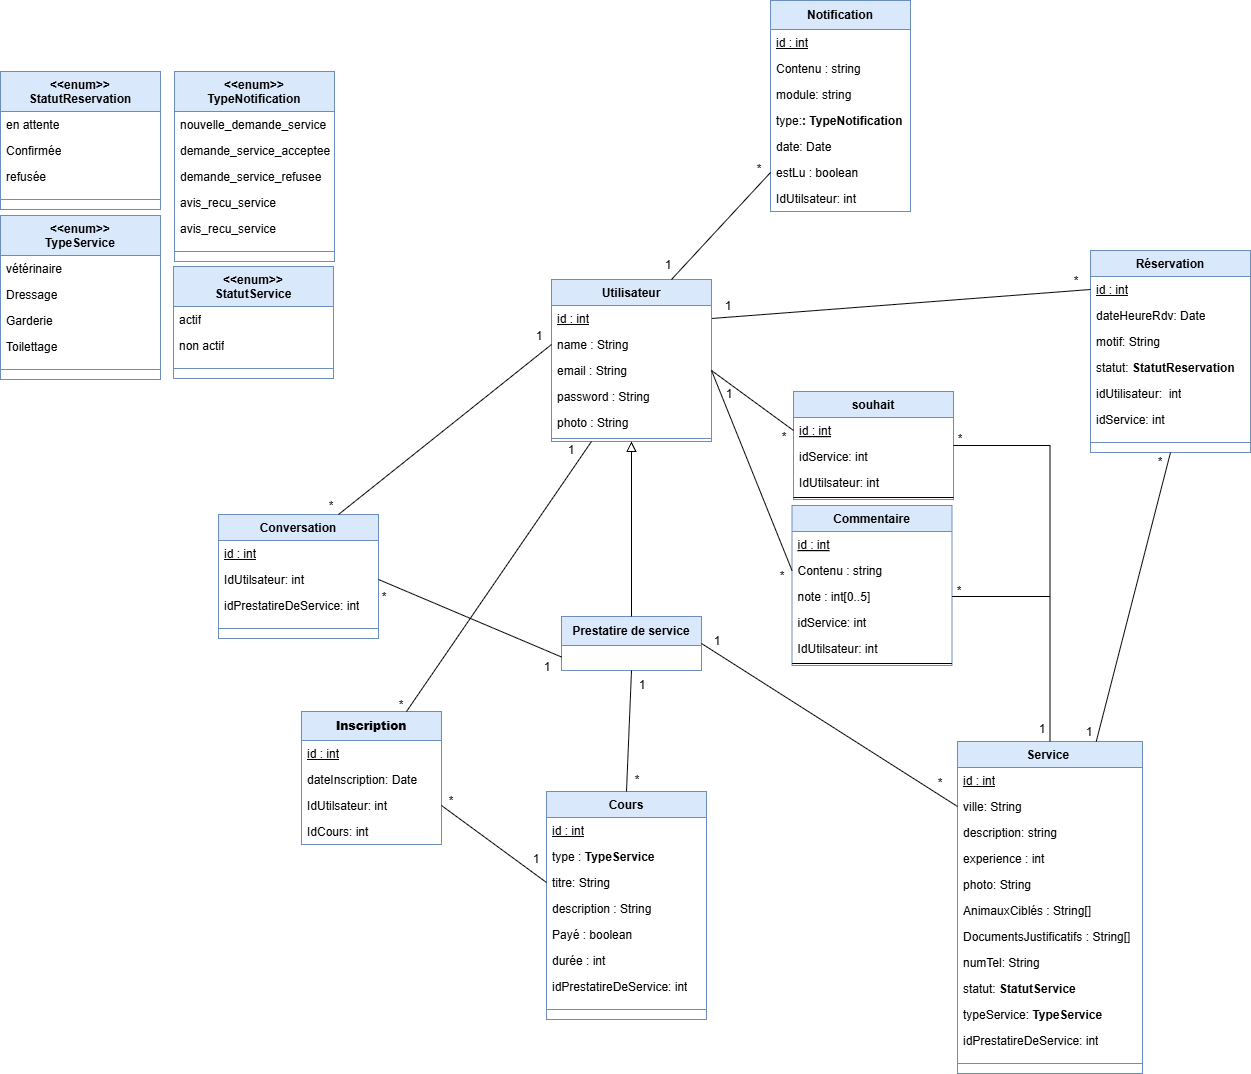
\includegraphics[width=18cm, height=20cm, keepaspectratio]{images/class digram anicare.png}
    \caption{Diagramme de classes de la sprint 5}
    \label{fig:class_diagram_sprint5}
\end{figure} 

\subsection{Diagrammes de séquence du sprint 5}

Cette section présente les diagrammes de séquence du cinquième sprint, qui illustrent les interactions entre les différents composants du système .  
\newpage 
\subsubsection{Diagramme de séquence : consultation  des services}

Cette figure illustre les interactions de l’utilisateur avec les services : consultation et filtrage (sans authentification), ainsi que les actions authentifiées comme les commentaires, les favoris (wishlist) et la réservation. Elle présente les échanges entre le frontend, l’API Gateway, le service AniCare, la base de données et le système de notification : 
\begin{figure}[H]
    \centering
    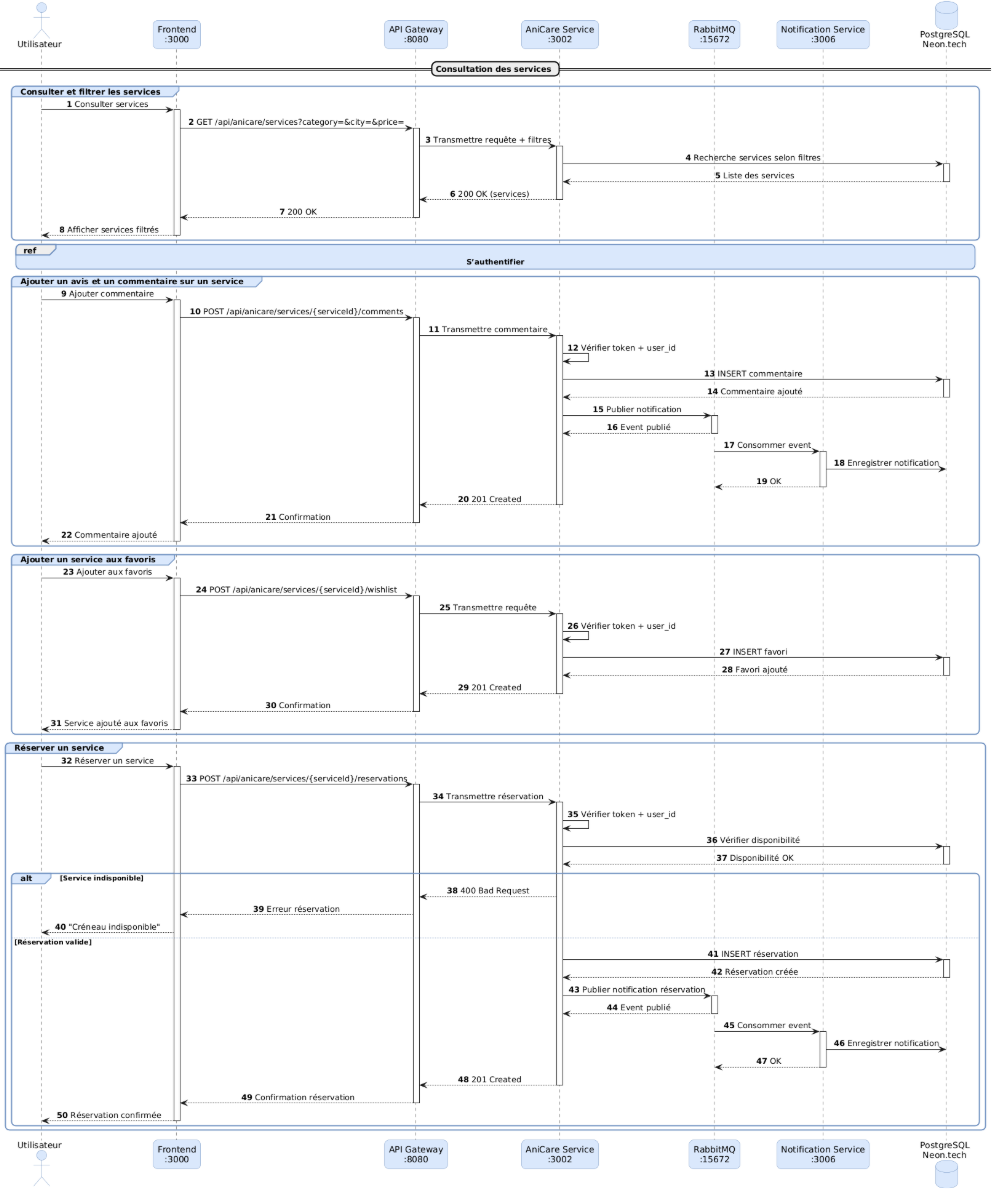
\includegraphics[width=0.85\textwidth]{images/consulter services sq.png}
    \caption{Diagramme de séquence : consultation  des services}
    \label{fig:services_utilisateur}
\end{figure}
\newpage 
\subsubsection{Diagramme de séquence : gestion des services}

Cette figure illustre les interactions du prestataire de service avec le système pour la gestion de ses services, notamment la création, la modification et la suppression. Elle met en évidence les échanges entre le frontend, l’API Gateway, le service AniCare et la base de données : 
\begin{figure}[H]
    \centering
    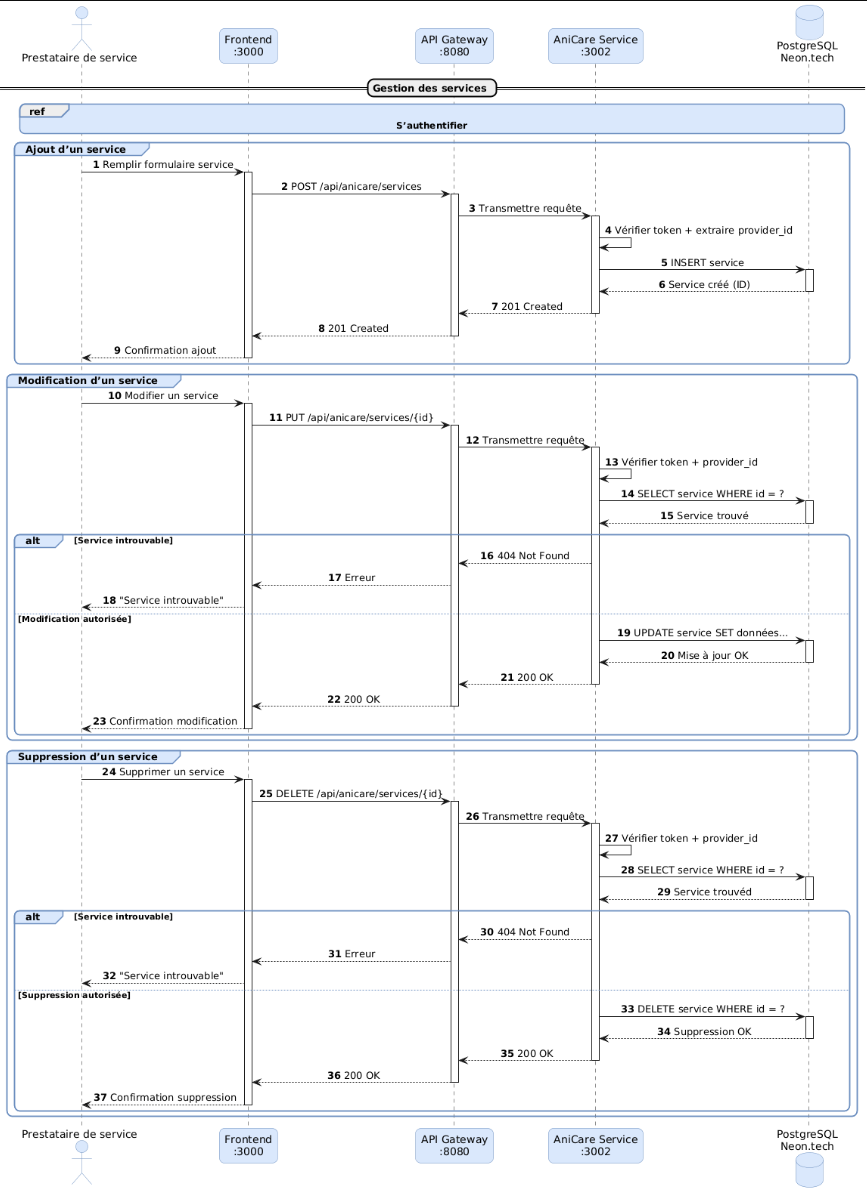
\includegraphics[width=0.8\textwidth]{images/gerer mes services sq.png}
    \caption{Diagramme de séquence : gestion des services}
    \label{fig:services_prestataire}
\end{figure}
\newpage 
\subsubsection{Diagramme de séquence : gestion des réservations reçues}

Cette figure illustre les interactions du prestataire de service pour la consultation, l’acceptation ou le refus des réservations reçues, ainsi que l’affichage de son emploi du temps. Elle met en évidence les échanges entre le frontend, l’API Gateway, le service AniCare, la base de données et le système de notification : 

\begin{figure}[H]
    \centering
    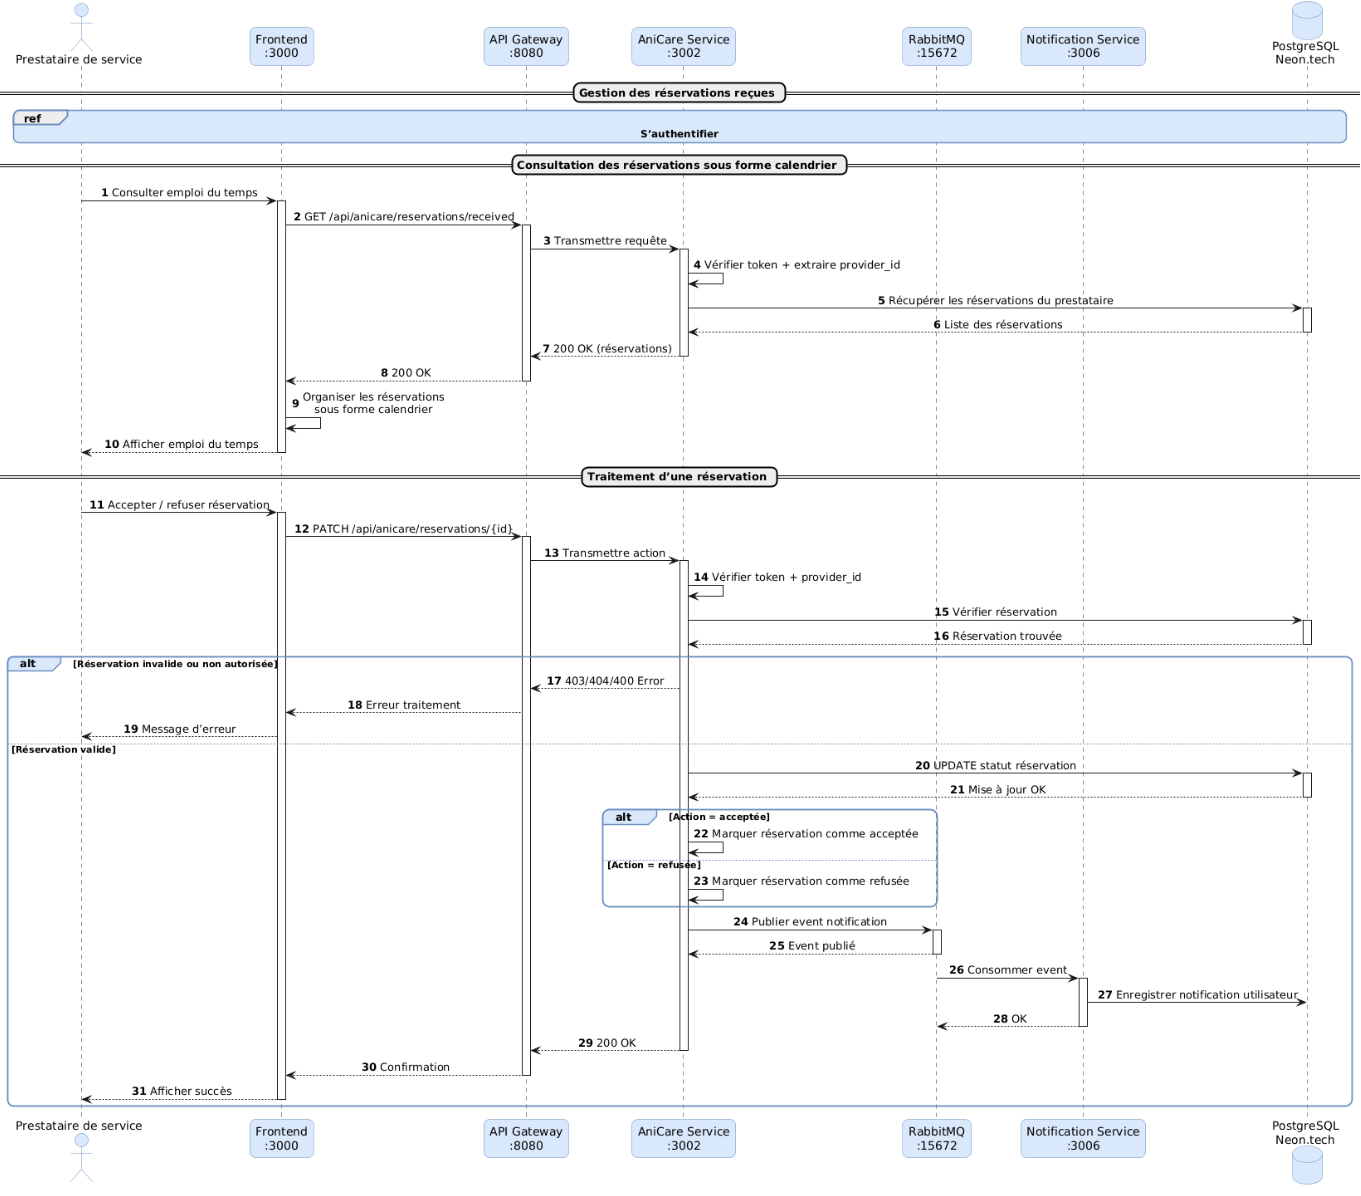
\includegraphics[width=1\textwidth]{images/gerer reservations recus sq.png}
    \caption{Diagramme de séquence : gestion des réservations reçues}
    \label{fig:reservations_prestataire}
\end{figure}
\newpage
\subsection{Réalisation du sprint 5} 
\subsubsection{Interface d’accueil AniCare} 
Cette figure illustre l’interface d’accueil du
module AniCare :  
\begin{figure}[h!]
    \centering
    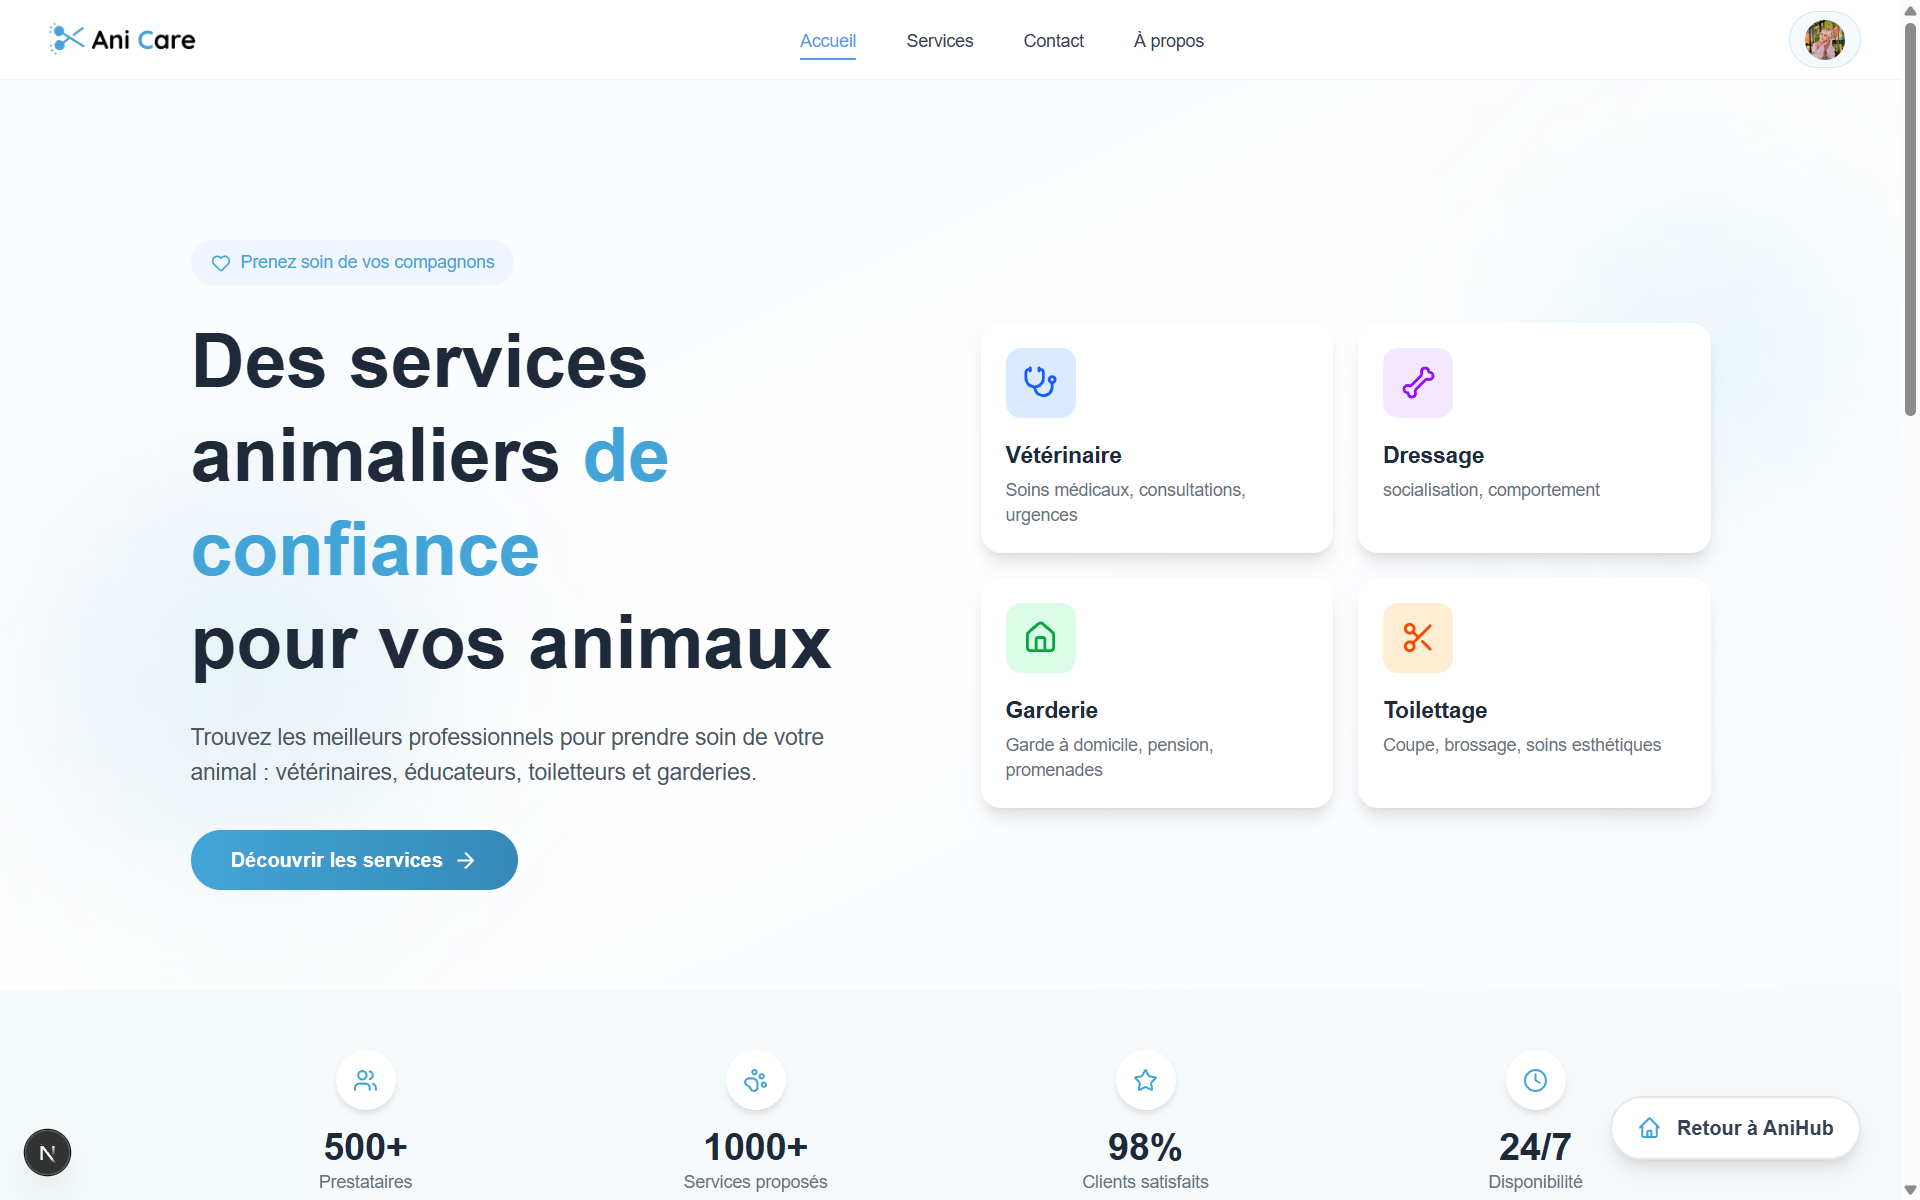
\includegraphics[width=0.73\textwidth]{images/acceuil anicare.png}
    \caption{Interface d’accueil du module AniCare}
\end{figure}  
\subsubsection{Interface de publication d’un service}   
Cette interface illustre le formulaire de publication d’un service dans le module AniCare : 
\begin{figure}[h!]
    \centering
    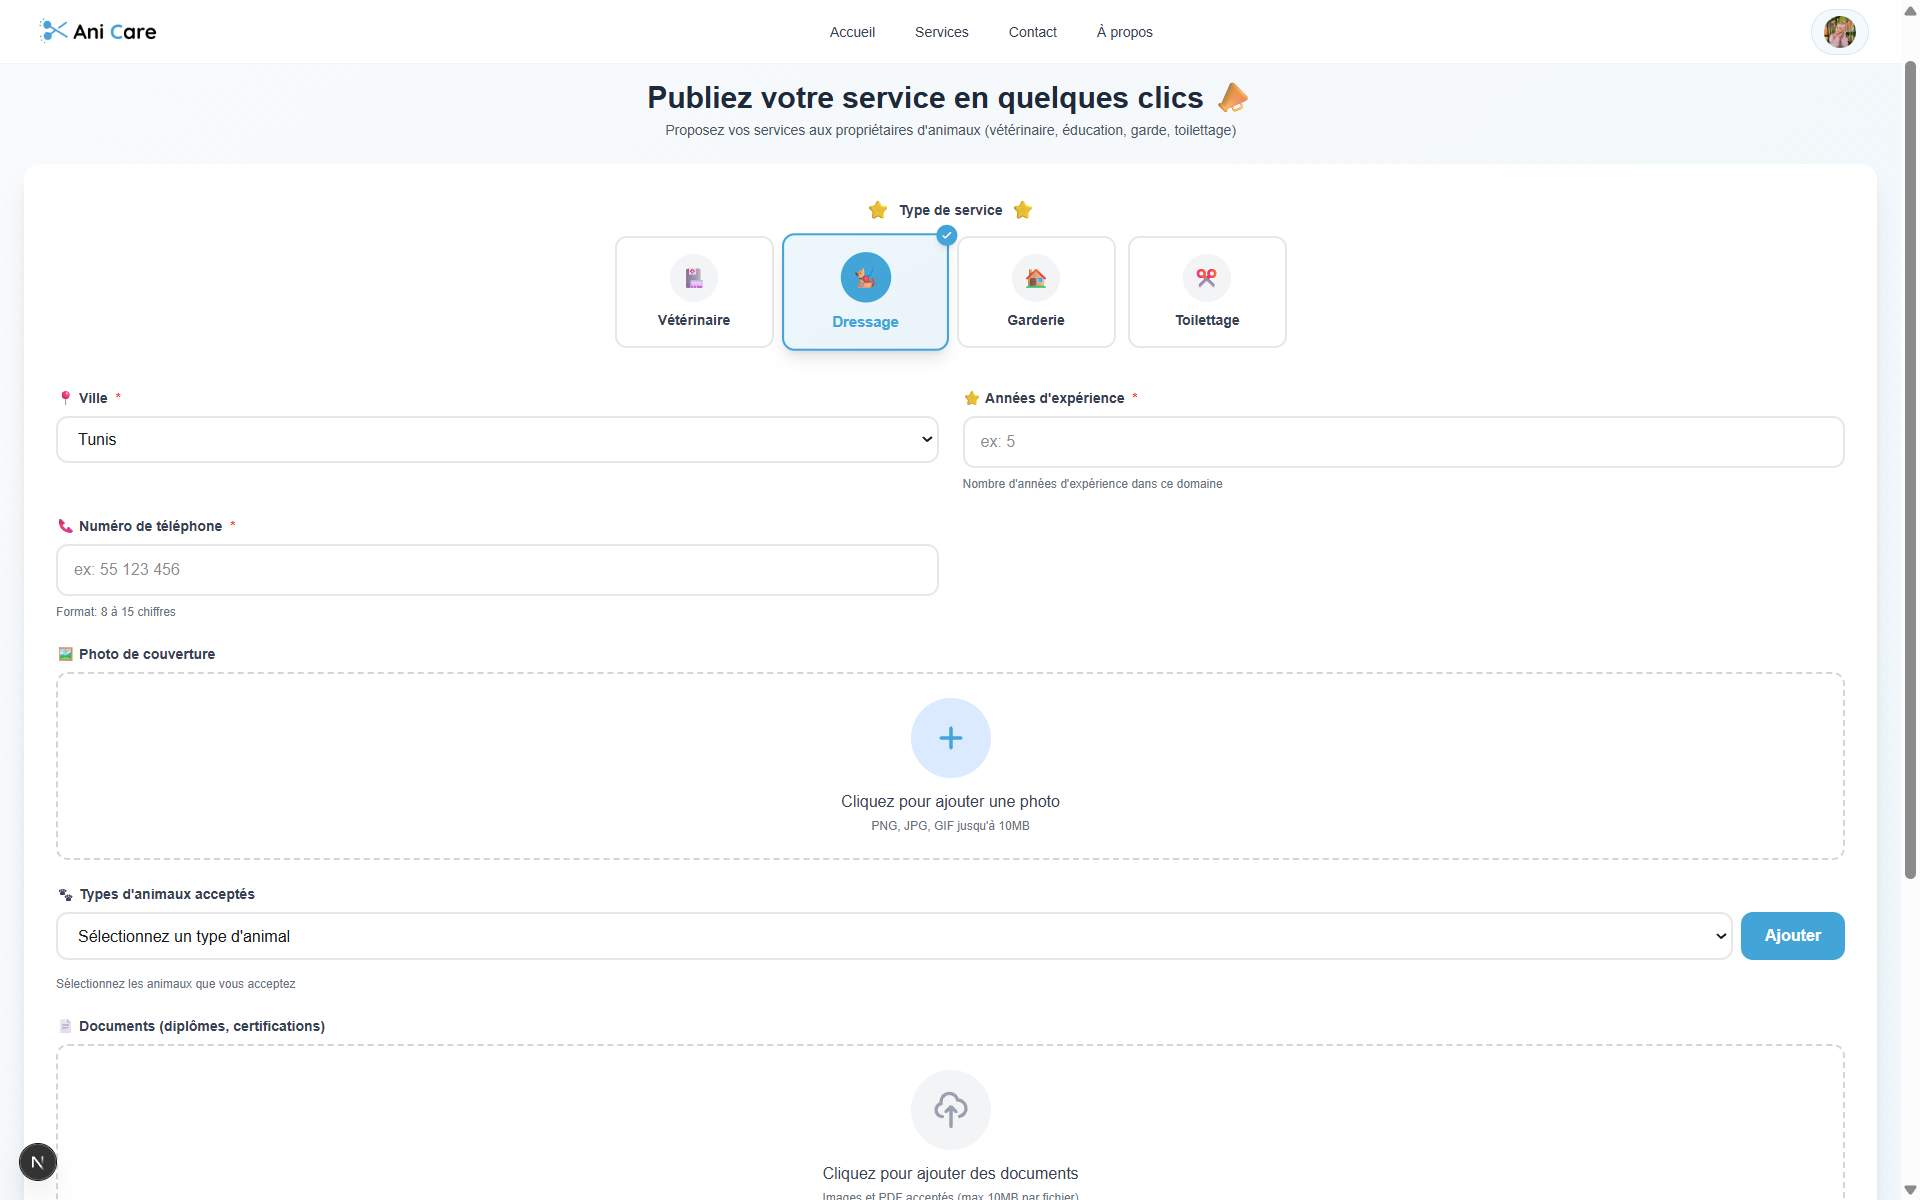
\includegraphics[width=0.73\textwidth]{images/publier mon service.png}
    \caption{Interface de publication d’un service}
\end{figure}  
\newpage 

\subsubsection{Interface des annonces de services dans AniCare}  
Cette interface illustre les services proposés par les prestataires dans le module AniCare : 
\begin{figure}[h!]
    \centering
    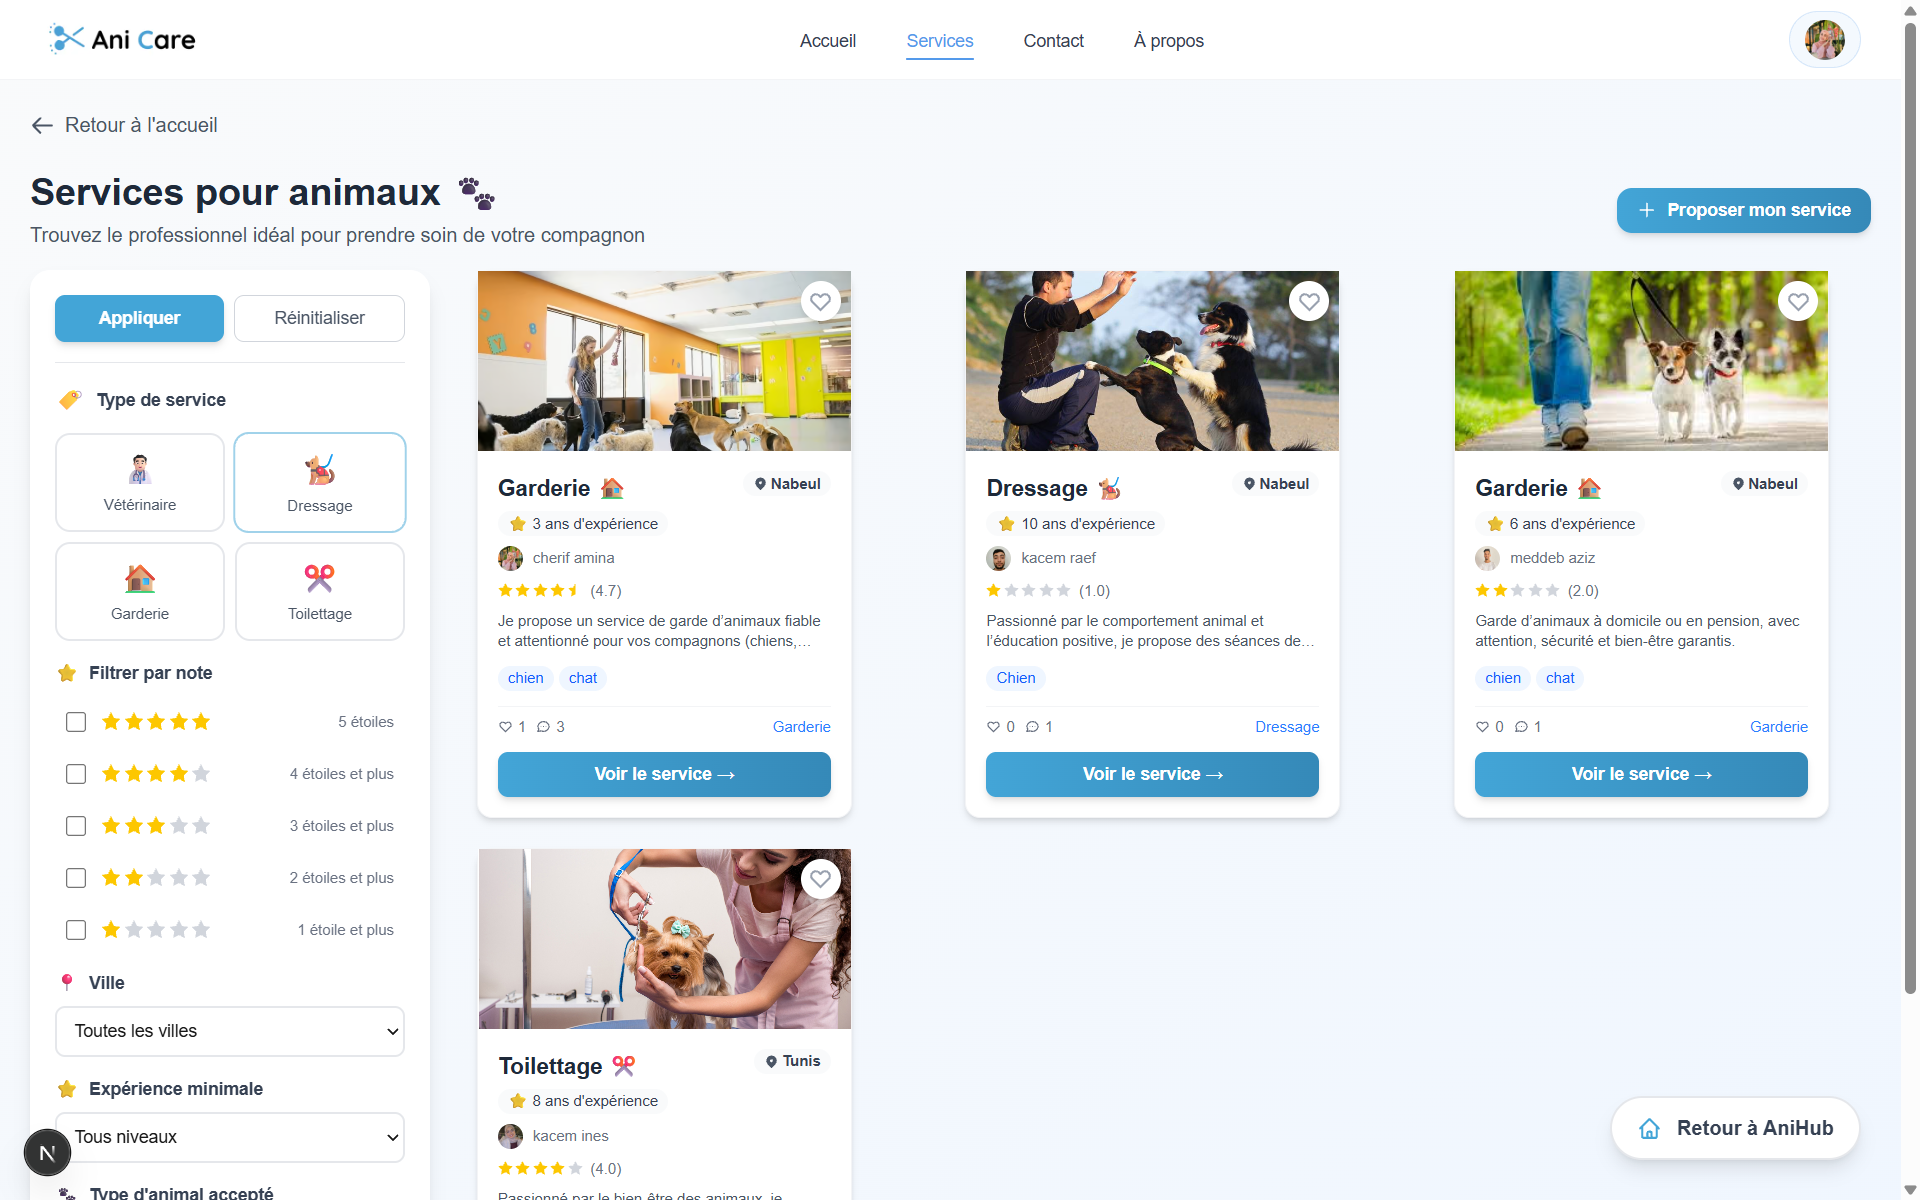
\includegraphics[width=0.73\textwidth]{images/services.png}
    \caption{Interface des annonces de services dans AniCare}
\end{figure}   

\subsubsection{Interface des détails d’un service} 
Cette interface illustre les détails d’un service proposé dans le module AniCare : 
\begin{figure}[h!]
    \centering
    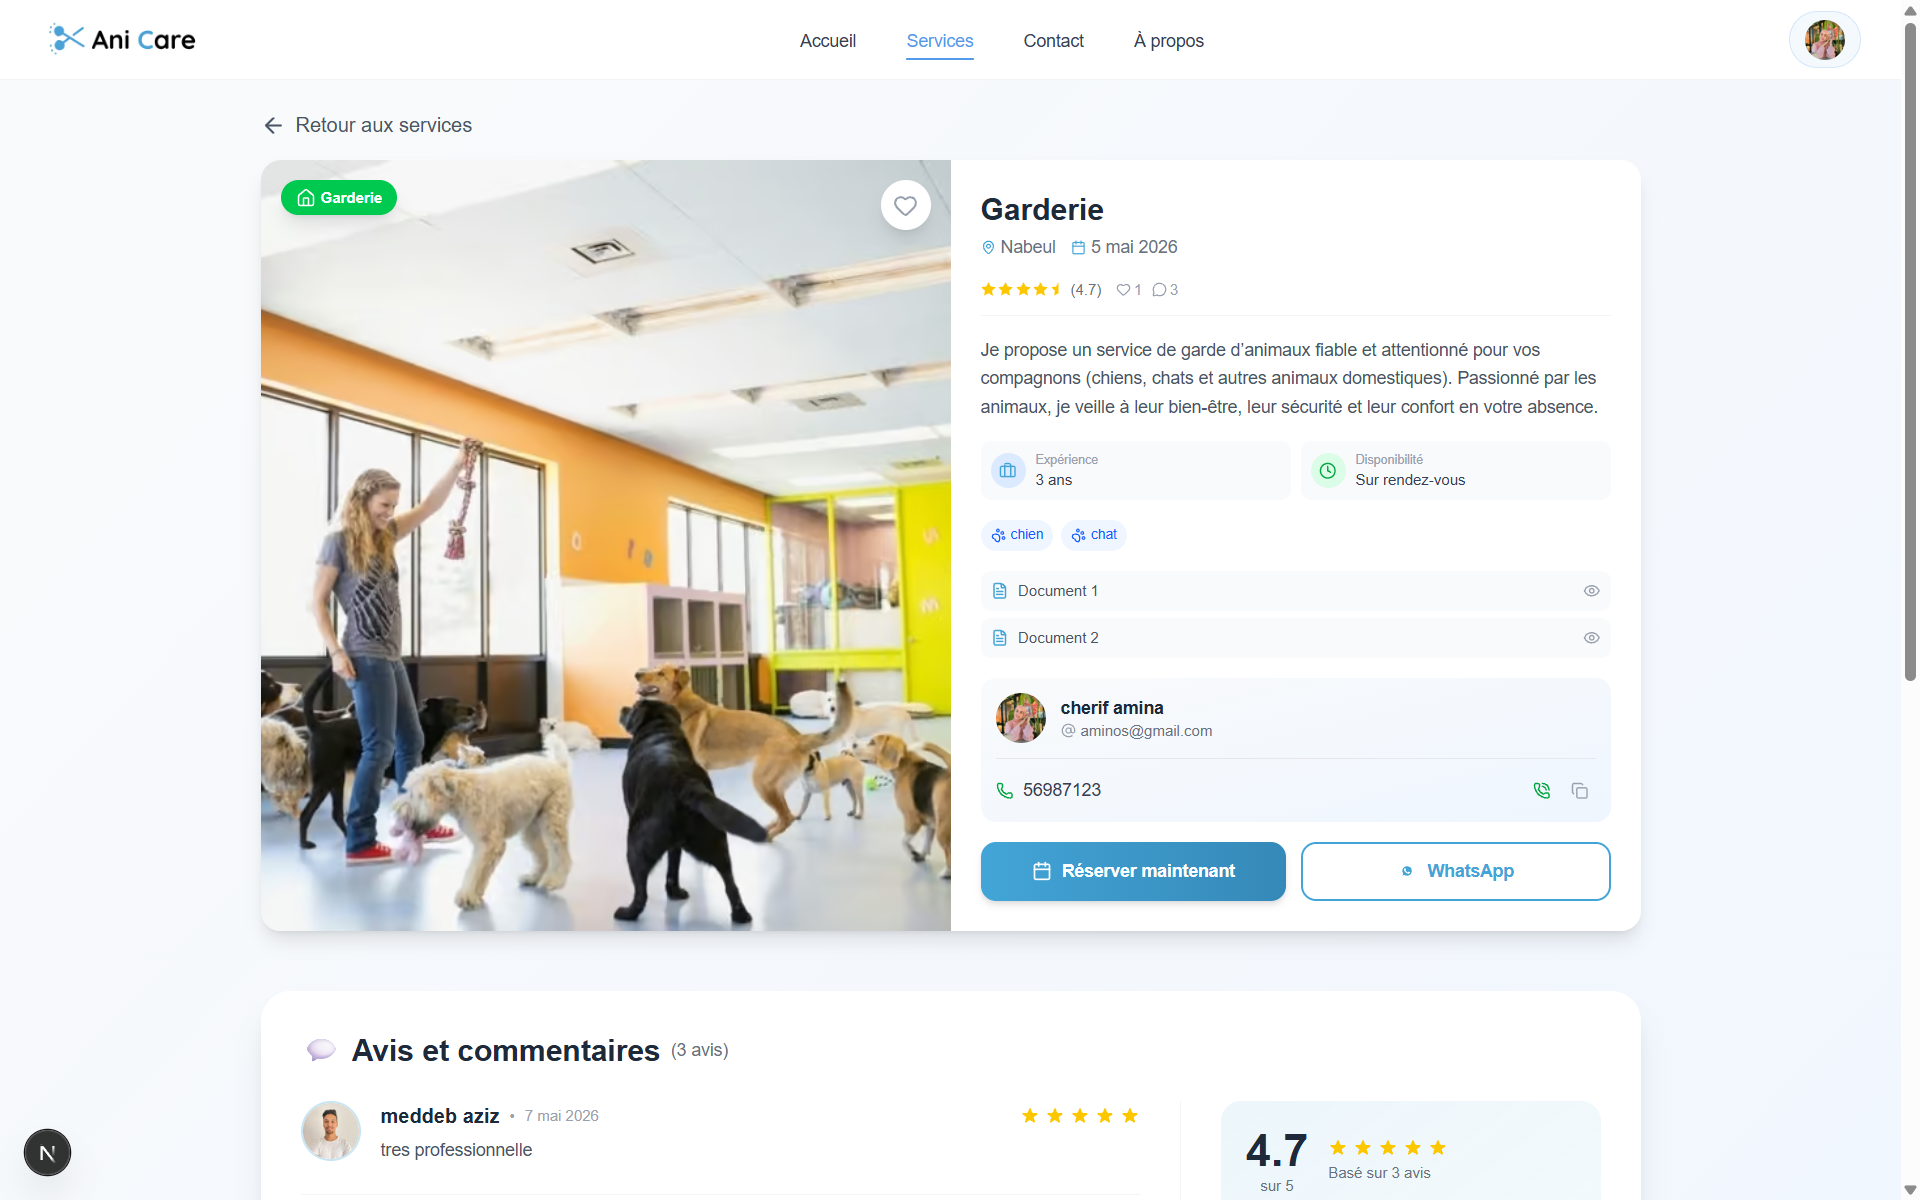
\includegraphics[width=0.73\textwidth]{images/details services.png}
    \caption{Interface des détails d’un service}
\end{figure}   
\newpage 
\subsubsection{Interface de réservation d’un service pour un demandeur} 
Cette interface illustre le processus de réservation d’un service par un demandeur dans le module AniCare : 
\begin{figure}[h!]
    \centering
    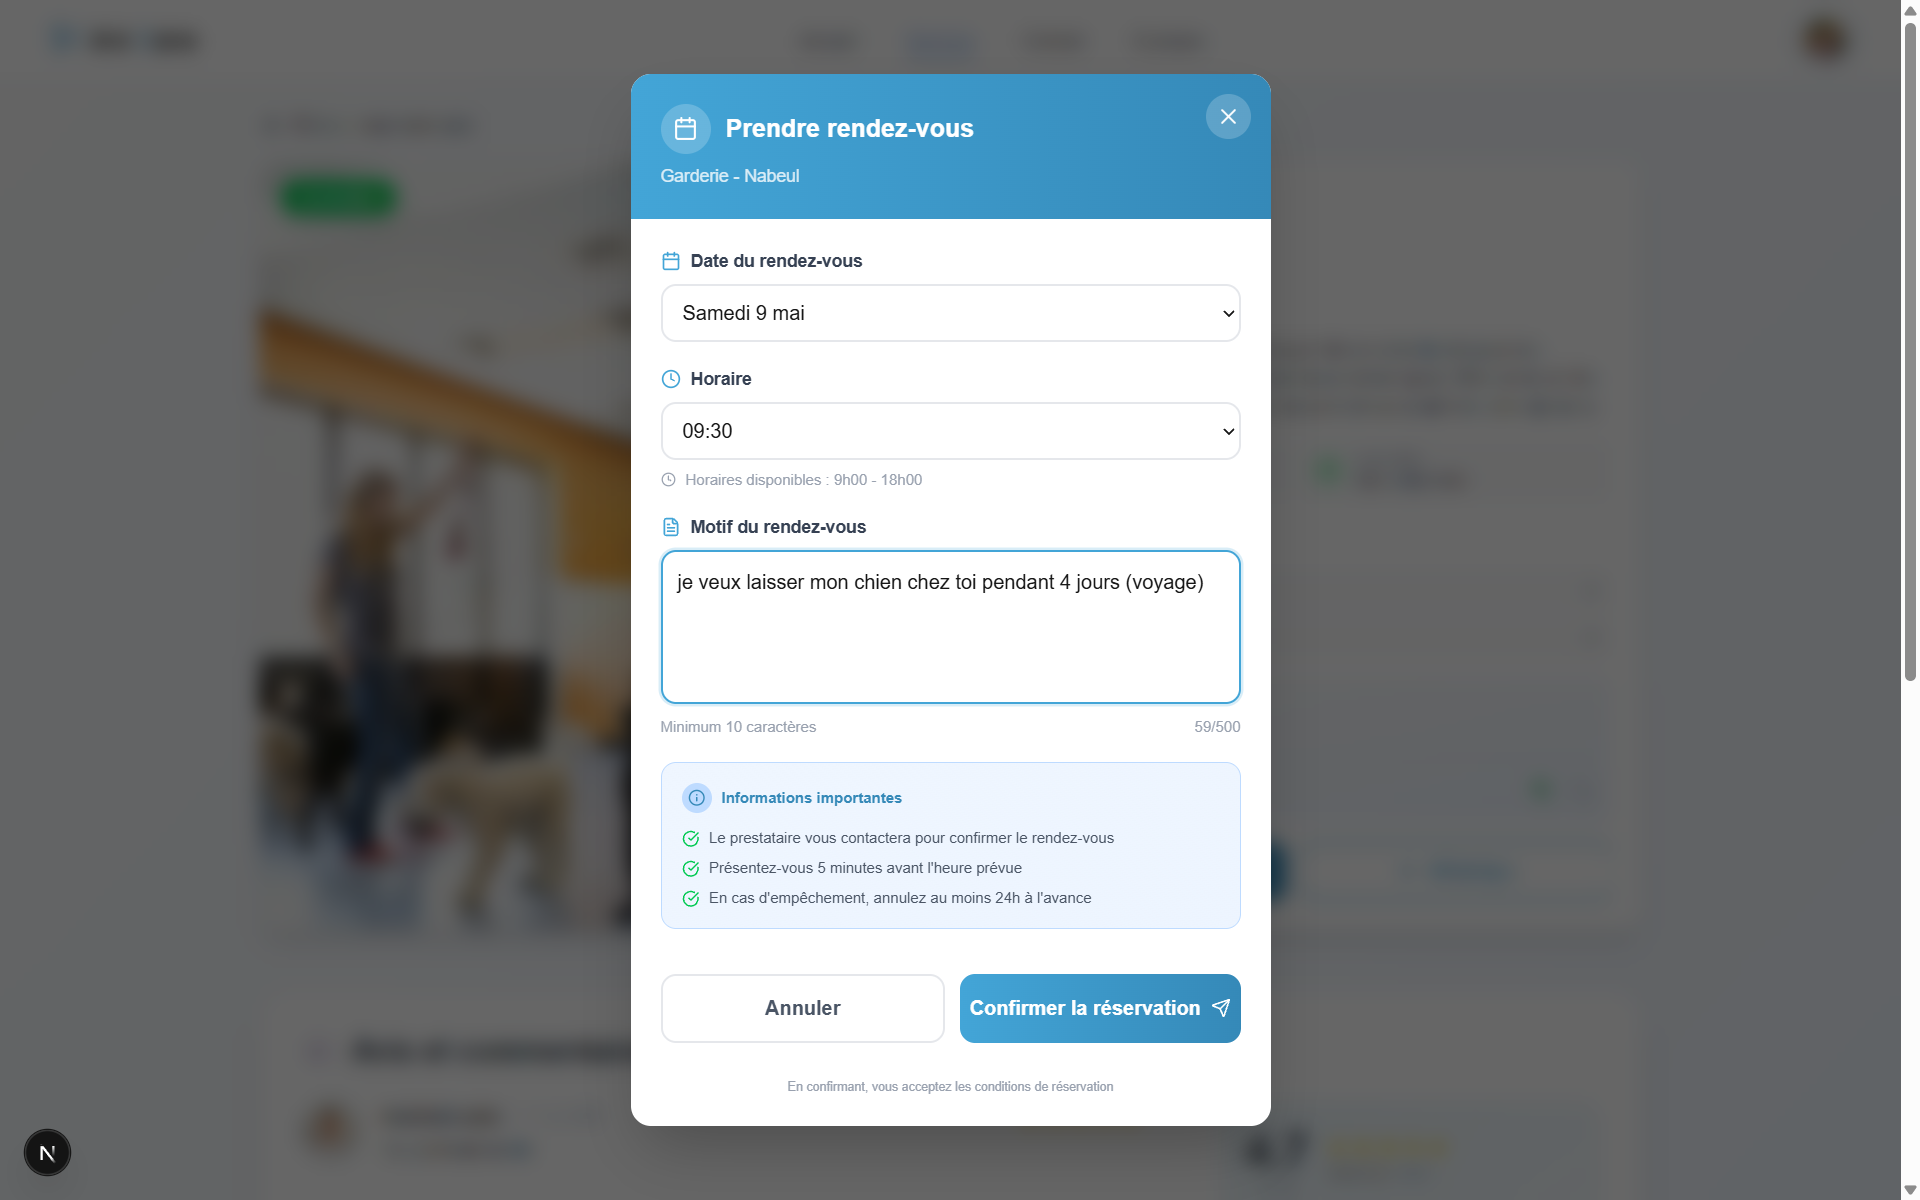
\includegraphics[width=0.73\textwidth]{images/interface reservation.png}
    \caption{Interface de réservation d’un service pour un demandeur}
\end{figure}   

\subsubsection{Interface des avis des clients sur un service}  
Cette interface illustre les avis et évaluations laissés par les clients pour un service dans le module AniCare : 

\begin{figure}[h!]
    \centering
    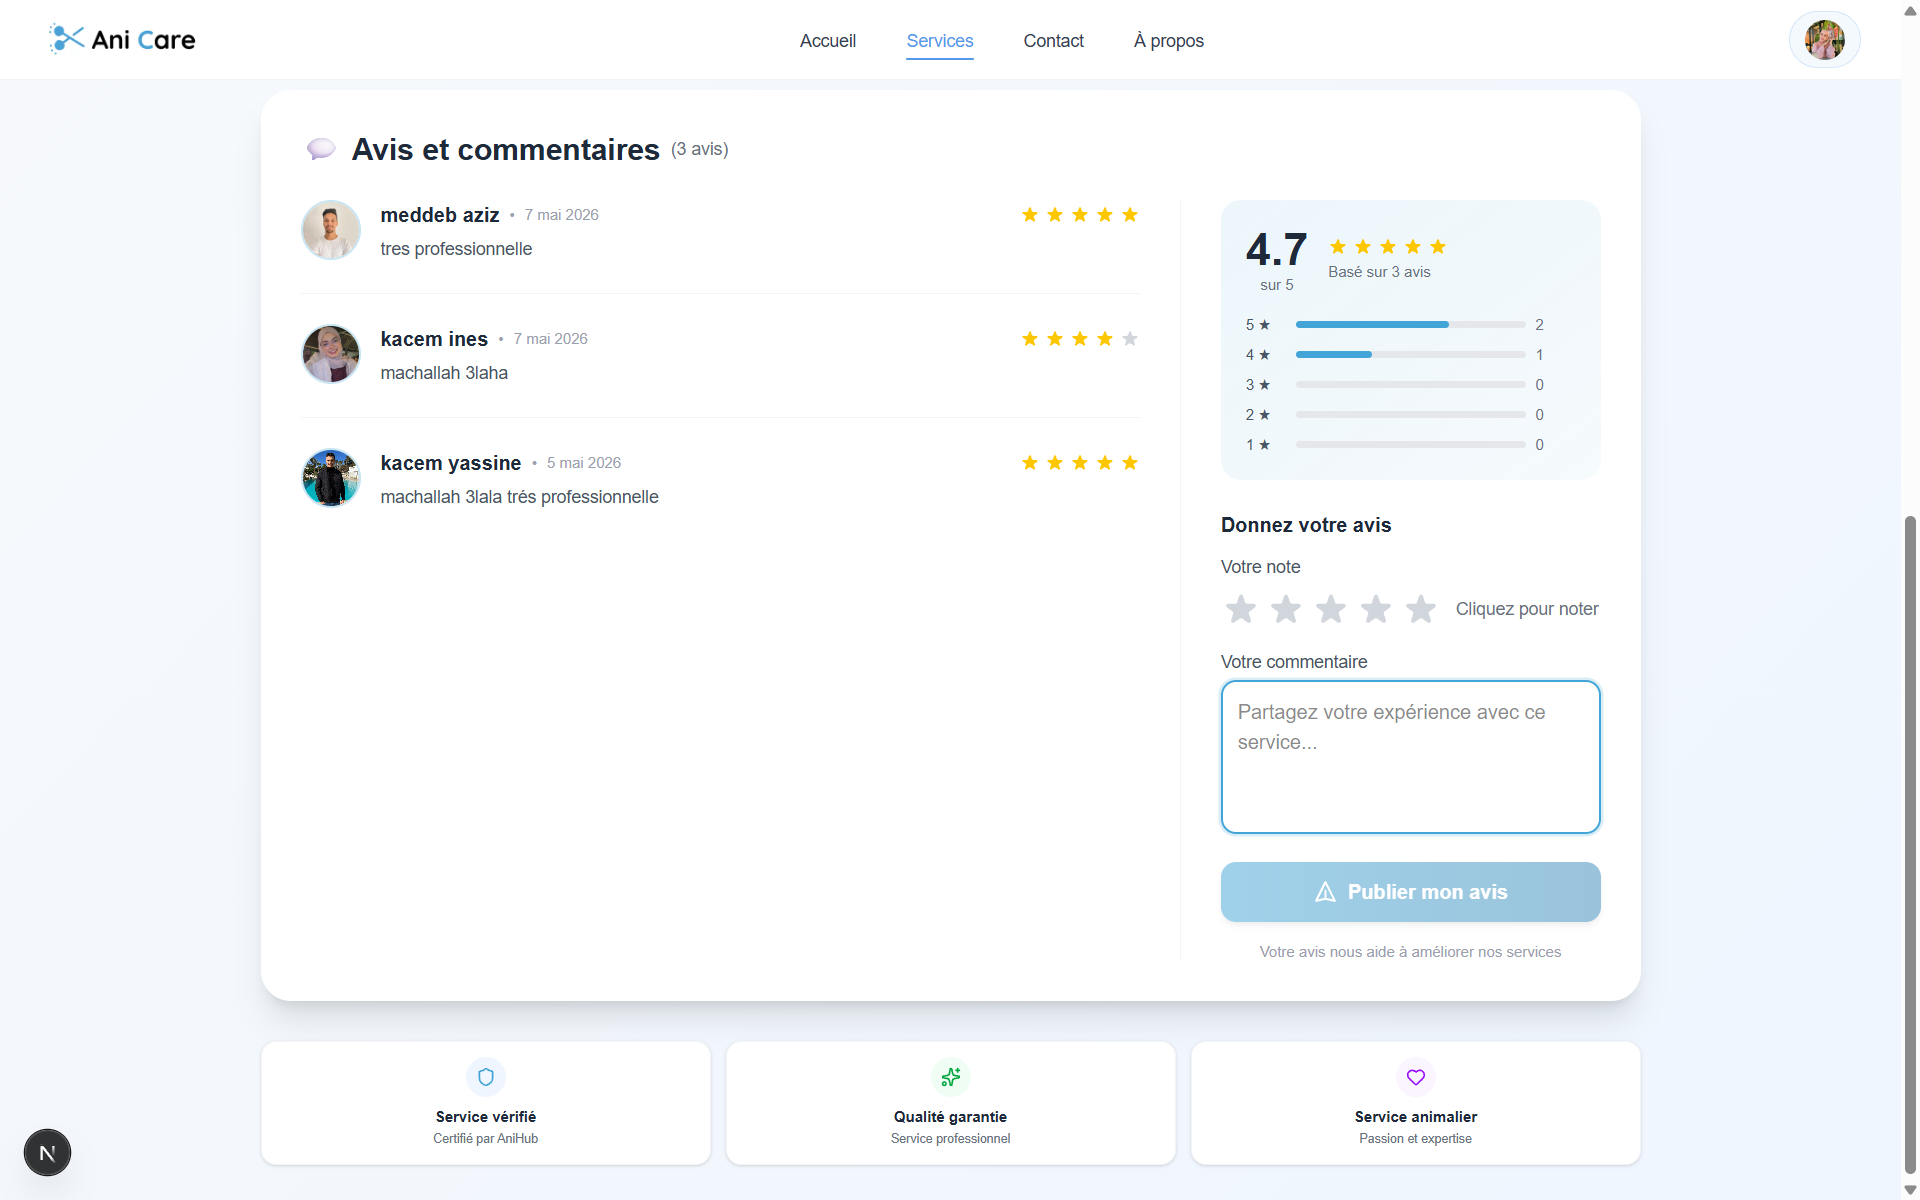
\includegraphics[width=0.73\textwidth]{images/interface avis.png}
    \caption{Interface des avis des clients sur un service}
\end{figure}  
\newpage 
\subsubsection{Interface de l’espace AniCare pour un prestataire} 
Cette interface illustre l’espace personnel du prestataire dans le module AniCare, lui permettant de gérer ses services et ses réservations : 
\begin{figure}[h!]
    \centering
    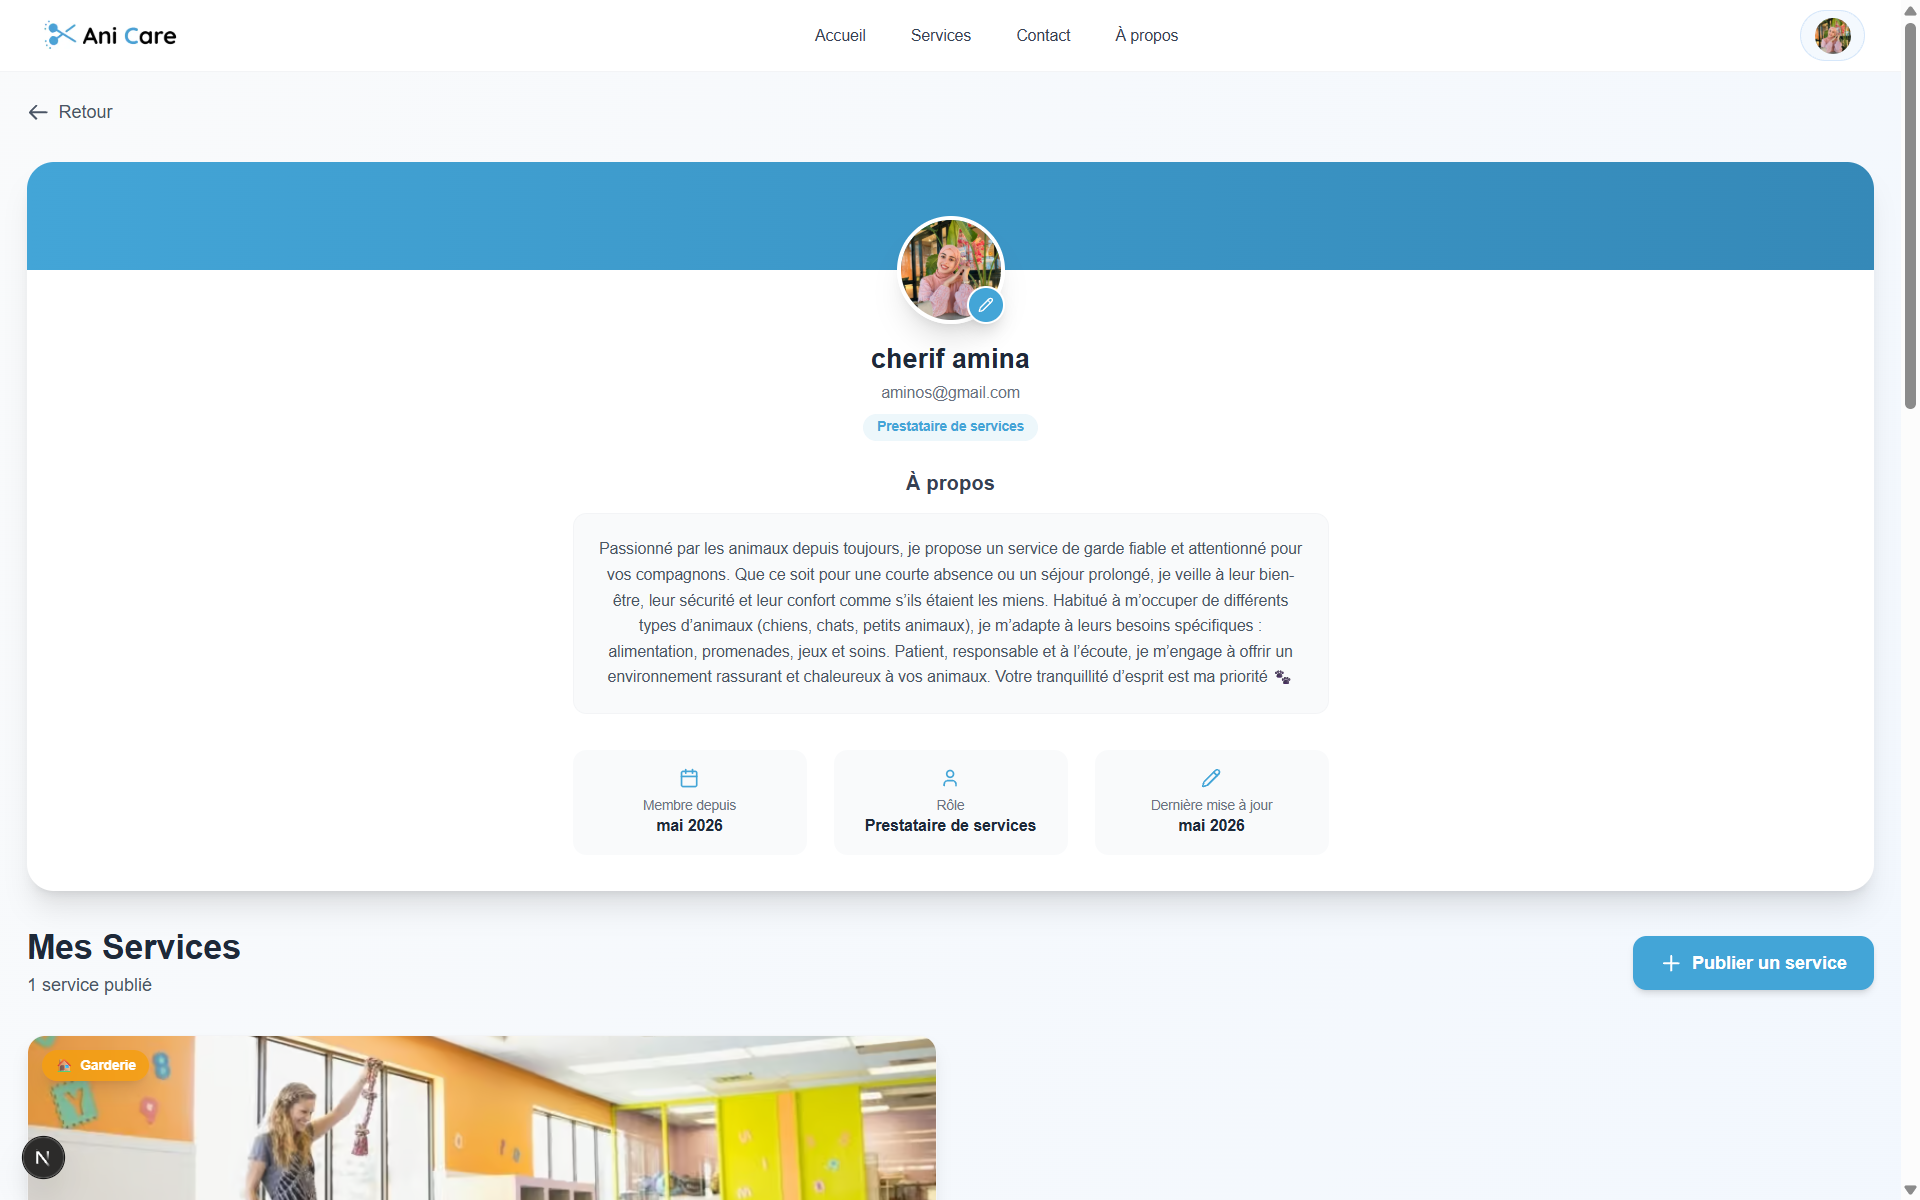
\includegraphics[width=0.73\textwidth]{images/espace anicare.png}
    \caption{Interface de l’espace AniCare pour un prestataire}
\end{figure}    
\subsubsection{Interfaces de modification et de suppression d’un service} 
Ces interfaces illustrent les fonctionnalités de modification et de suppression d’un service dans le module AniCare : 
\begin{figure}[h!]
    \centering
    
    \begin{minipage}{0.48\textwidth}
        \centering
        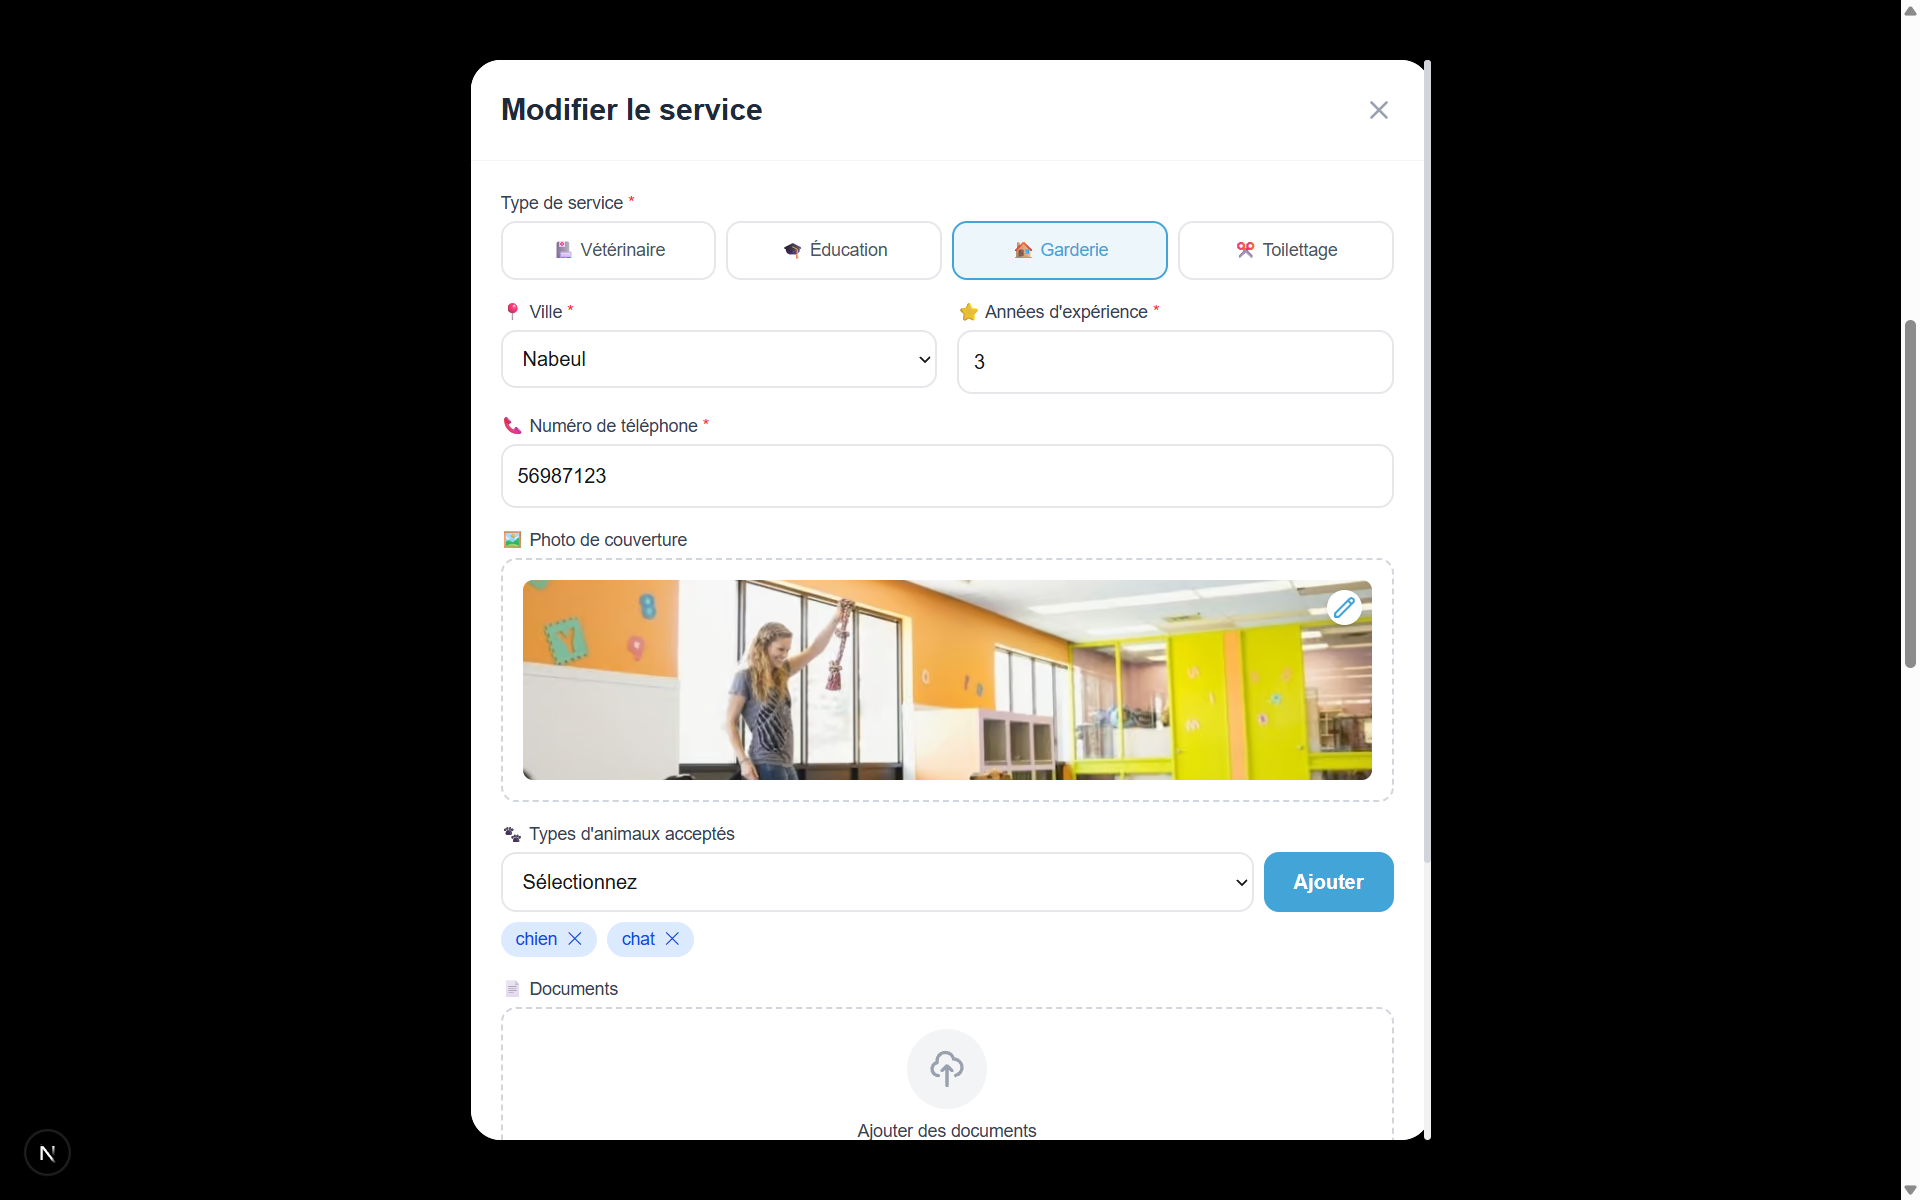
\includegraphics[width=\textwidth]{images/modifieer service.png}
        \caption{Interface modification service}
    \end{minipage}
    \hfill
    \begin{minipage}{0.48\textwidth}
        \centering
        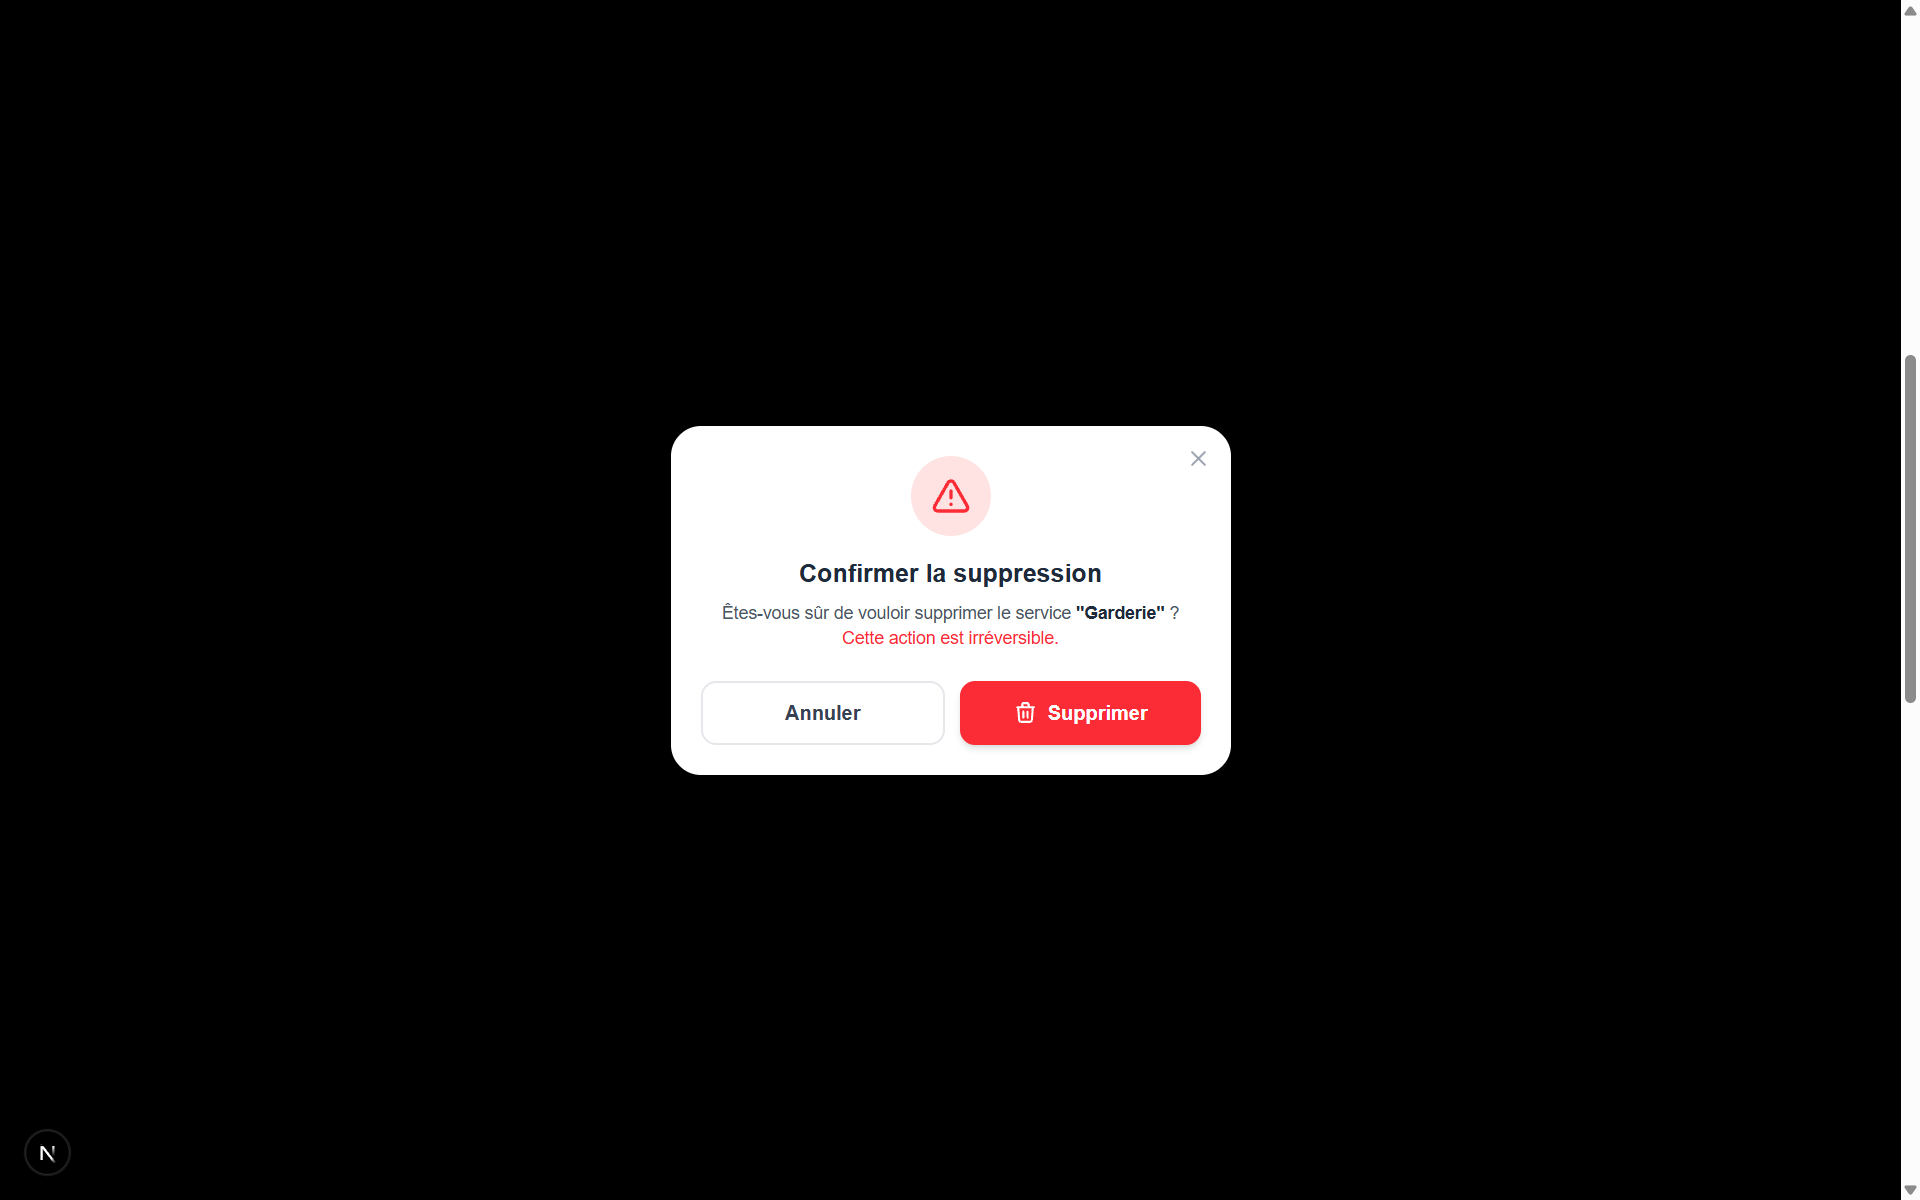
\includegraphics[width=\textwidth]{images/suppression service}
        \caption{Interface suppression service}
    \end{minipage}

\end{figure}  
\newpage 
\subsubsection{Interface de gestion des réservations reçues pour le prestataire} 
Cette interface illustre la gestion des réservations reçues par le prestataire dans le module AniCare : 
\begin{figure}[h!]
    \centering
    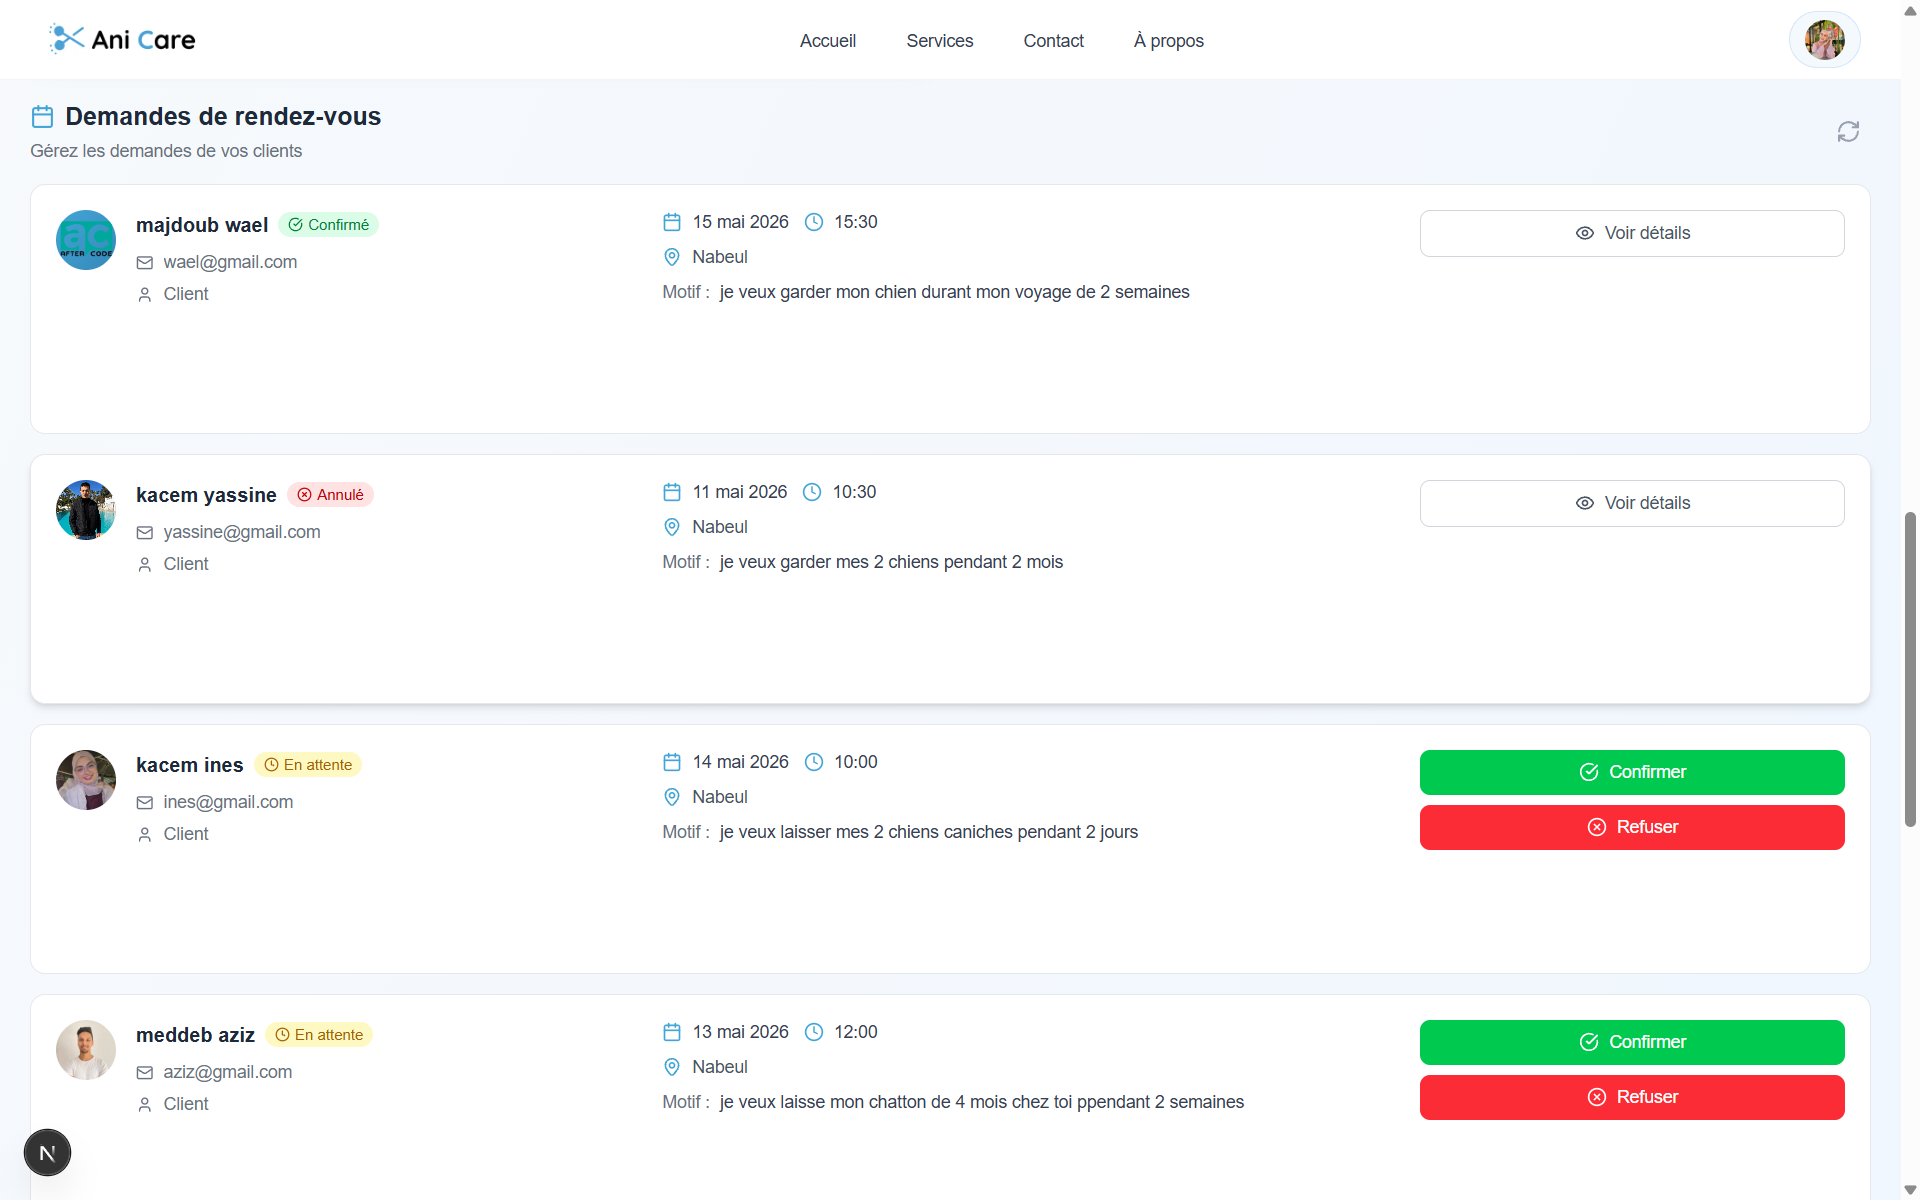
\includegraphics[width=0.73\textwidth]{images/mes reservation recus.png}
    \caption{Interface de gestion des réservations reçues pour le prestataire}
\end{figure}   
\subsubsection{Interface du planning du prestataire} 
Cette interface illustre le planning du prestataire dans le module AniCare, affichant ses horaires, jours et disponibilités : 
\begin{figure}[h!]
    \centering
    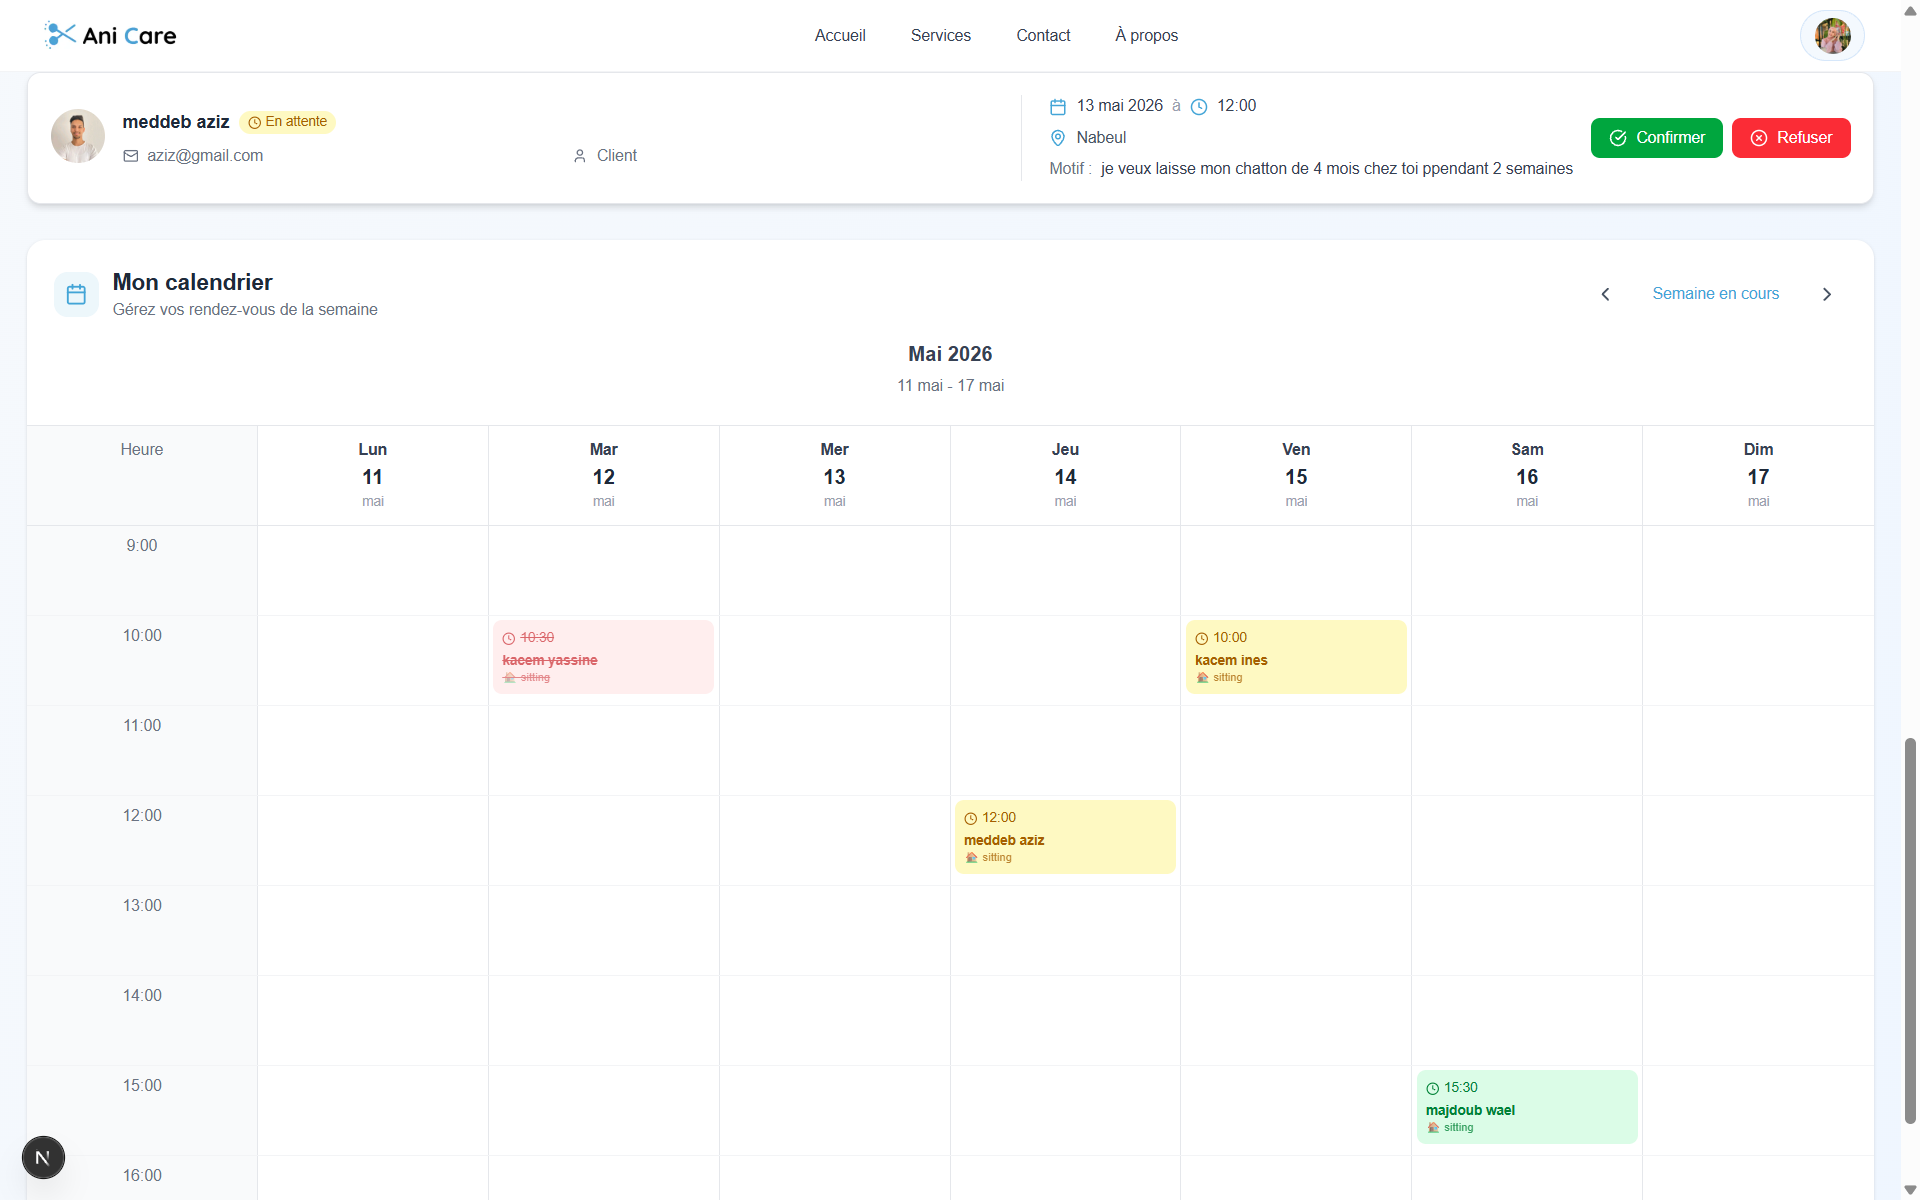
\includegraphics[width=0.73\textwidth]{images/mycalendar.png}
    \caption{Interface du planning du prestataire}
\end{figure}   
\newpage 
\subsubsection{Interface de gestion des réservations envoyées pour le demandeur} 
Cette interface illustre la gestion des réservations envoyées par le demandeur dans le module AniCare :
\begin{figure}[h!]
    \centering
    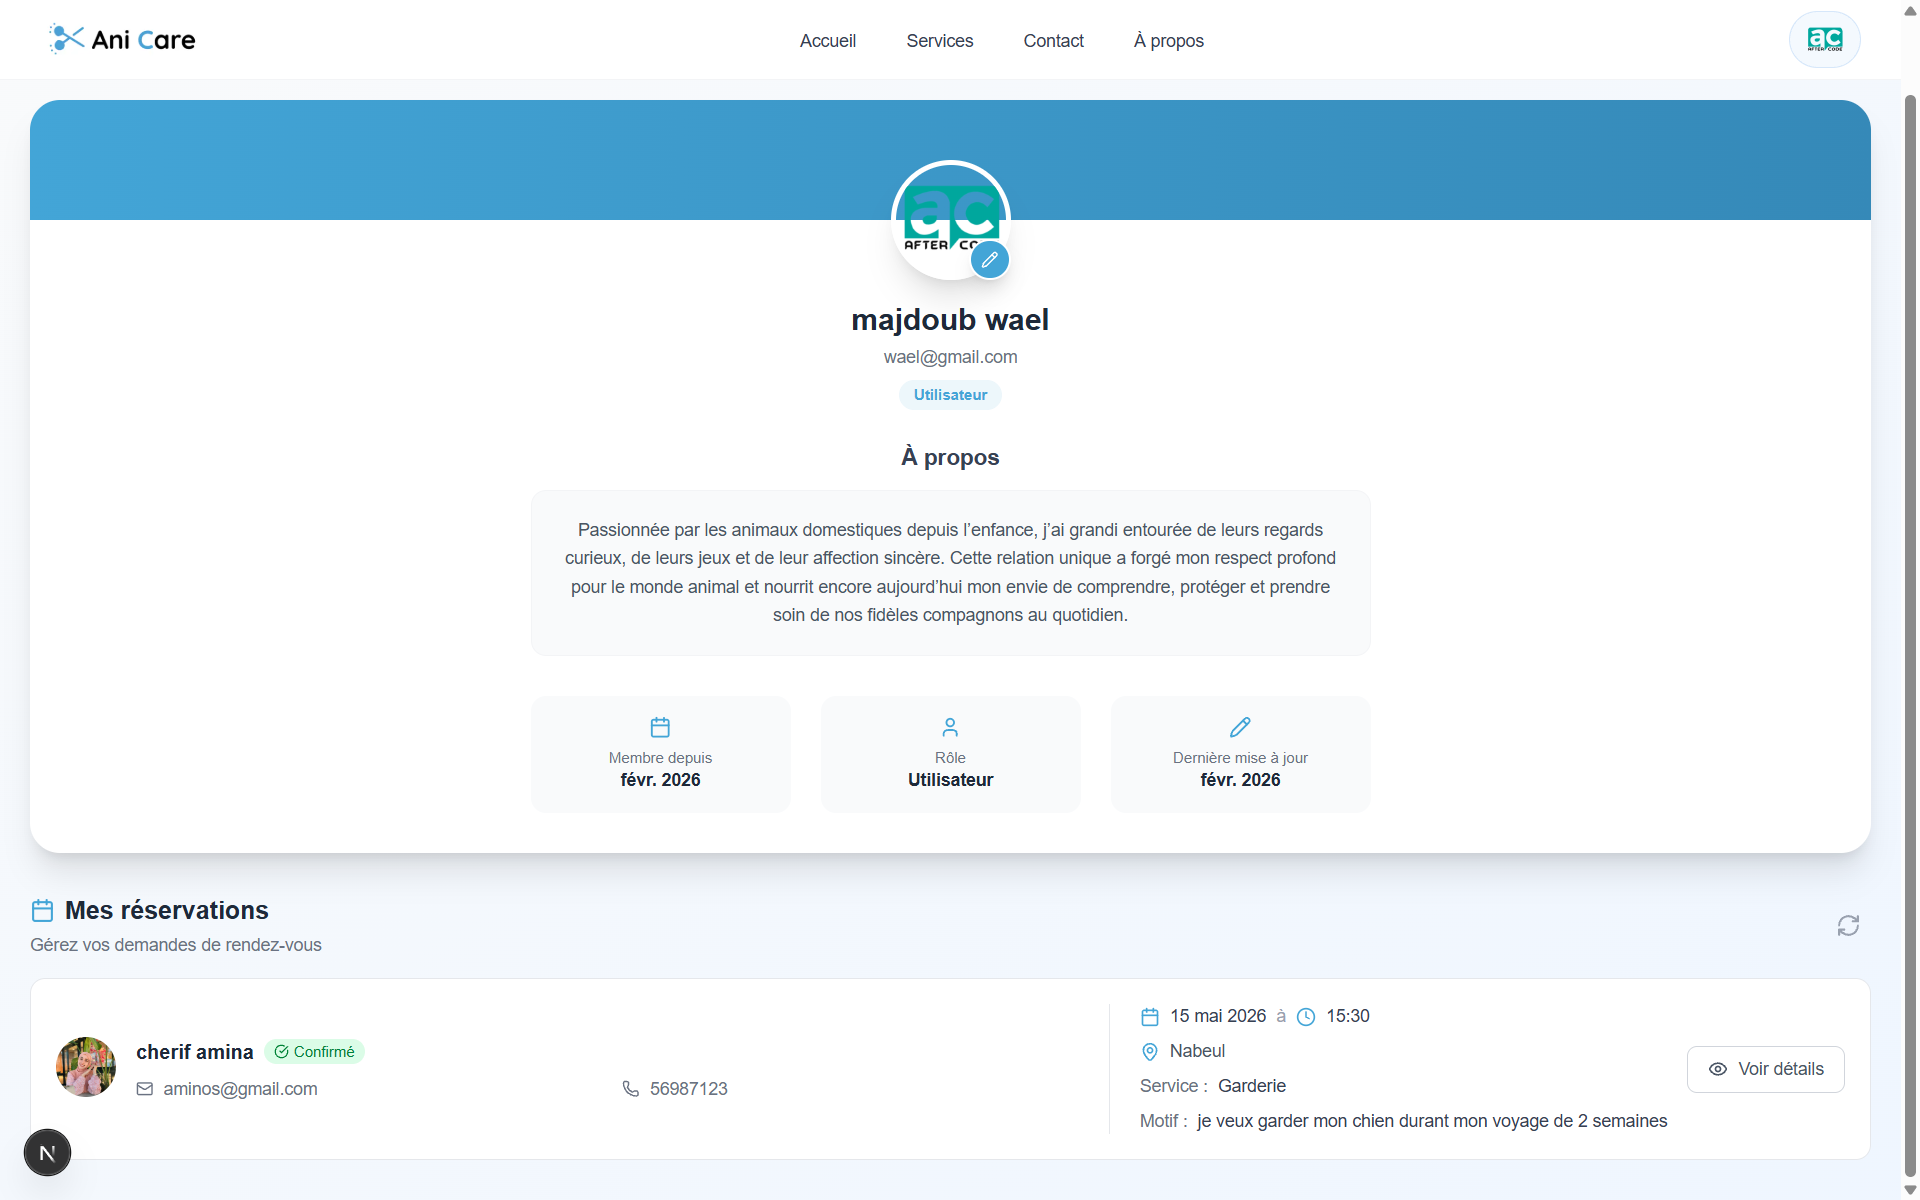
\includegraphics[width=0.73\textwidth]{images/mes reservations.png}
    \caption{Interface de gestion des réservations envoyées pour le demandeur}
\end{figure}   
\subsubsection{Interface des notifications d’acceptation de réservation et de rendez-vous} 
Cette interface illustre les notifications d’acceptation de réservation et de rendez-vous dans le module AniCare : 
\begin{figure}[h!]
    \centering
    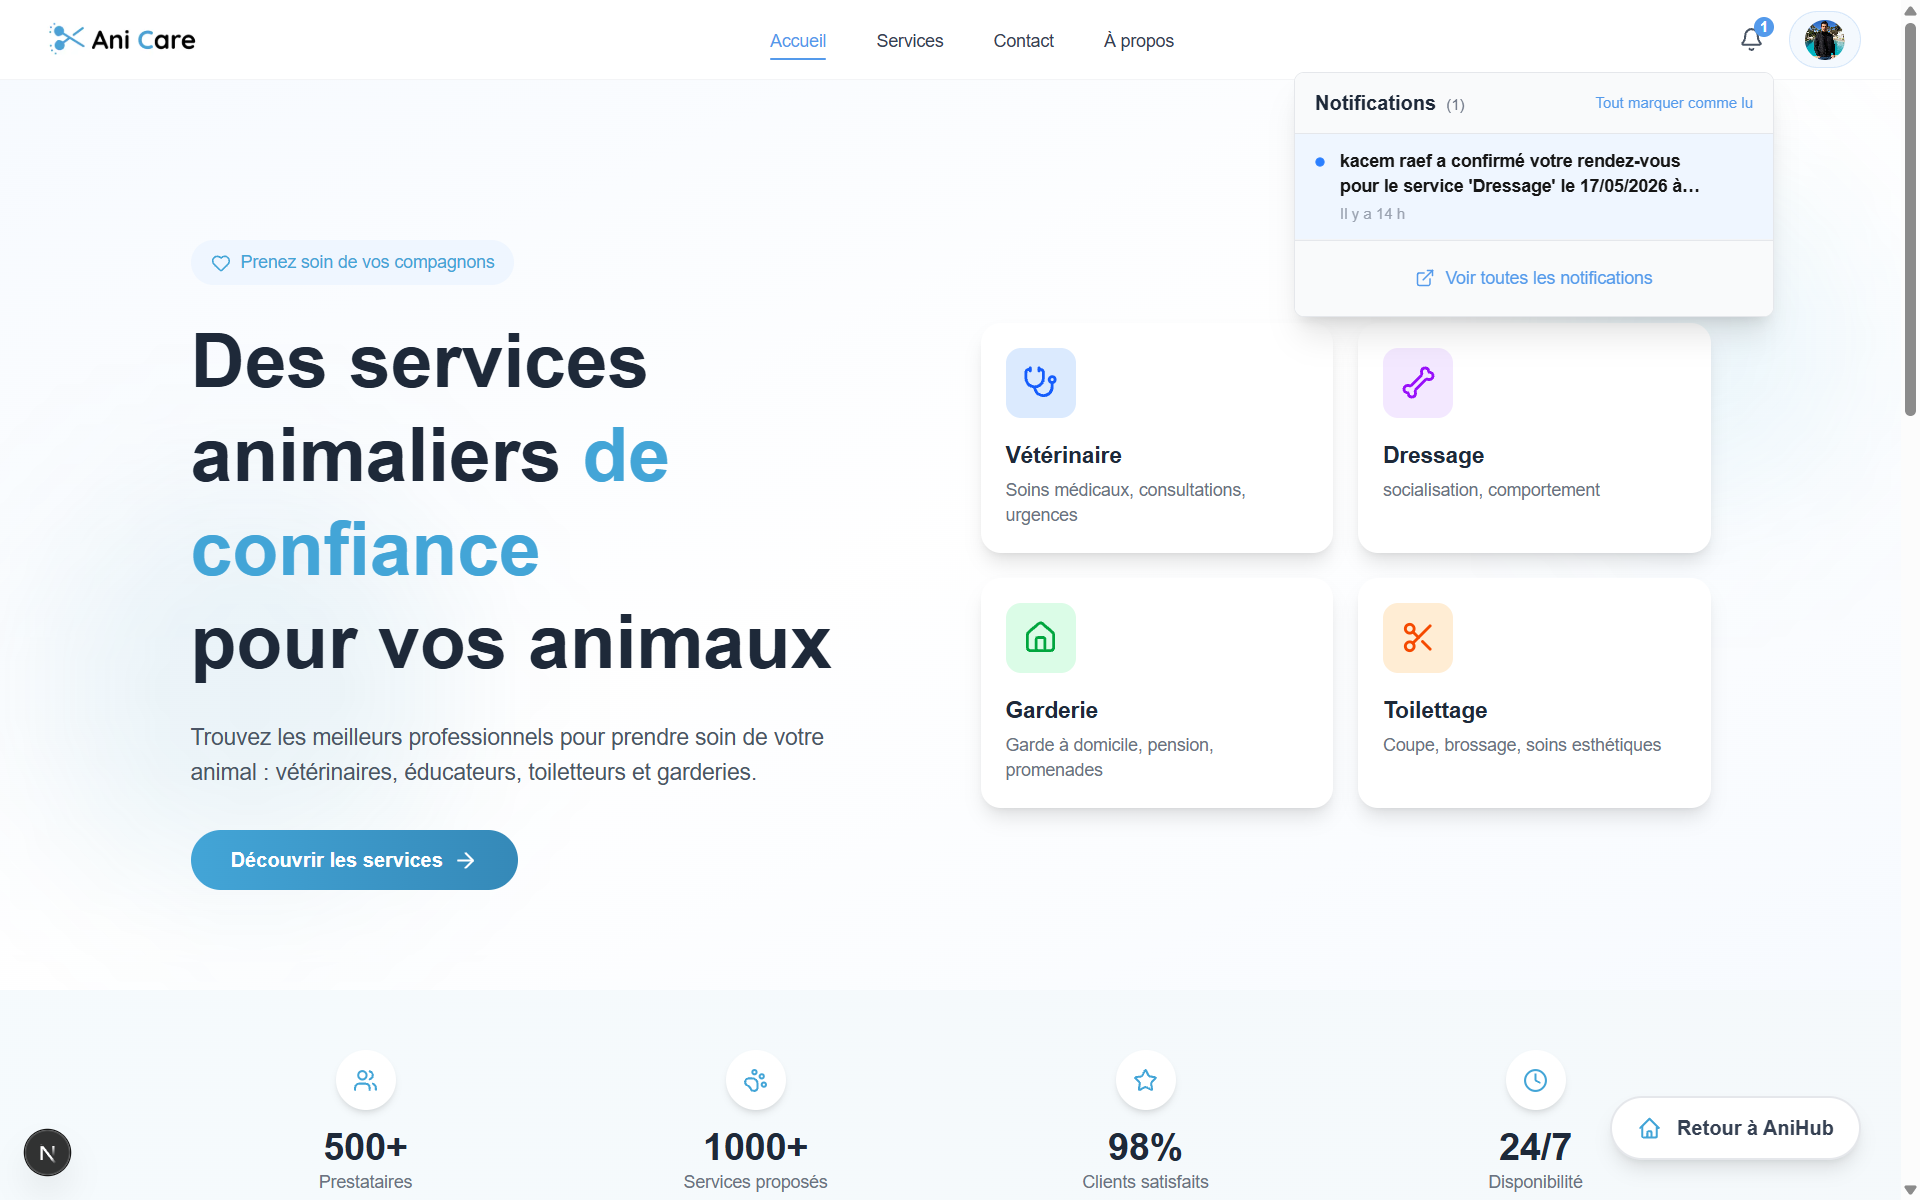
\includegraphics[width=0.73\textwidth]{images/notif anicare.png}
    \caption{Interface des notifications d’acceptation de réservation et de rendez-vous}
\end{figure}   

\newpage
\section{Sprint 6 : Conteneurisation, CI/CD, Déploiement Cloud et Monitoring} 
Dans ce sprint, d’une durée de \textbf{3 semaines}, nous nous sommes concentrés sur la mise en place de l’environnement DevOps de l’application AniHub. Cette étape a permis de conteneuriser les microservices à l’aide de Docker, d’assurer leur orchestration avec Kubernetes et de déployer l’application sur Google Cloud Platform (GCP). Nous avons également mis en œuvre un pipeline CI/CD avec GitHub Actions afin d’automatiser les phases de build et de déploiement. Enfin, un système de monitoring basé sur Grafana et Prometheus a été intégré afin de superviser les performances et la disponibilité des microservices. 
\subsection{Sprint backlog} 
Le tableau suivant présente le Sprint Backlog du sprint 6 avec les user stories, les tâches associées et les efforts estimés : 
\begin{longtable}{|p{1cm}|p{4.7cm}|p{7cm}|p{1.3cm}|}

\caption{Sprint Backlog du sprint 6} \label{tab:sprint6-backlog} \\

\hline
\multicolumn{1}{|c|}{\cellcolor{coloranihub}\textbf{ID}} &
\multicolumn{1}{c|}{\cellcolor{coloranihub}\textbf{User Story}} &
\multicolumn{1}{c|}{\cellcolor{coloranihub}\textbf{Tâches}} &
\multicolumn{1}{c|}{\cellcolor{coloranihub}\textbf{Effort}} \\
\hline
\endfirsthead

\hline
\multicolumn{1}{|c|}{\cellcolor{coloranihub}\textbf{ID}} &
\multicolumn{1}{c|}{\cellcolor{coloranihub}\textbf{User Story}} &
\multicolumn{1}{c|}{\cellcolor{coloranihub}\textbf{Tâches}} &
\multicolumn{1}{c|}{\cellcolor{coloranihub}\textbf{Effort}} \\
\hline
\endhead

% ===================== US61 =====================
\multirow{5}{2cm}{US61}
& \multirow{5}{5cm}{Conteneuriser les microservices avec Docker afin de garantir un environnement d’exécution stable et portable.}
& Création des Dockerfile pour chaque microservice & 1 j \\
\cline{3-4}
& & Build des images Docker & 0.5 j \\
\cline{3-4}
& & Push des images vers Docker Hub & 0.5 j \\
\cline{3-4}
& & Configuration de Docker Compose pour l’environnement local & 0.5 j \\
\cline{3-4}
& & Vérification de l’exécution des conteneurs & 0.5 j \\
\hline

% ===================== US62 =====================
\multirow{5}{2cm}{US62}
& \multirow{5}{5cm}{Déployer les microservices sur Kubernetes afin d’assurer l’orchestration et la disponibilité de l’application.}
& Création des fichiers Deployment et Service Kubernetes & 1 j \\
\cline{3-4}
& & Configuration des pods et replicas & 0.5 j \\
\cline{3-4}
& & Mise en place des Ingress pour l’accès aux services & 0.5 j \\
\cline{3-4}
& & Déploiement sur le cluster Kubernetes & 0.5 j \\
\cline{3-4}
& & Tests de communication entre microservices & 0.5 j \\
\hline

% ===================== US63 =====================
\multirow{4}{2cm}{US63}
& \multirow{4}{5cm}{Déployer l’application sur Google Cloud Platform (GCP) afin de rendre la plateforme accessible en ligne.}
& Création du cluster Kubernetes sur GCP & 1 j \\
\cline{3-4}
& & Configuration de l’environnement cloud & 0.5 j \\
\cline{3-4}
& & Déploiement des microservices sur GCP & 0.5 j \\
\cline{3-4}
& & Validation de l’accès externe & 0.5 j \\
\hline

% ===================== US64 =====================
\multirow{4}{2cm}{US64}
& \multirow{4}{5cm}{Automatiser le build et le déploiement avec GitHub Actions afin d’assurer un processus CI/CD rapide et fiable.}
& Création du workflow GitHub Actions & 0.5 j \\
\cline{3-4}
& & Automatisation du build Docker & 0.5 j \\
\cline{3-4}
& & Pull des images depuis Docker Hub & 0.5 j \\
\cline{3-4}
& & Déploiement automatique sur Kubernetes & 0.5 j \\
\hline

% ===================== US65 =====================
\multirow{4}{2cm}{US65}
& \multirow{4}{5cm}{Surveiller les microservices avec Grafana afin de suivre les performances et détecter les anomalies du système.}
& Installation de Prometheus pour la collecte des métriques & 0.5 j \\
\cline{3-4}
& & Configuration de Grafana & 0.5 j \\
\cline{3-4}
& & Création des dashboards de monitoring & 0.5 j \\
\cline{3-4}
& & Surveillance des pods et ressources Kubernetes & 0.5 j \\
\hline
\end{longtable}  


\subsection{Conteneurisation des microservices avec Docker}  

\subsubsection{Création des fichiers Dockerfile}

Cette figure présente un exemple de Dockerfile du microservice \textit{AniMatch}, utilisé pour définir et automatiser la création d’une image Docker pour ce microservice :   

\begin{figure}[H]
    \centering
    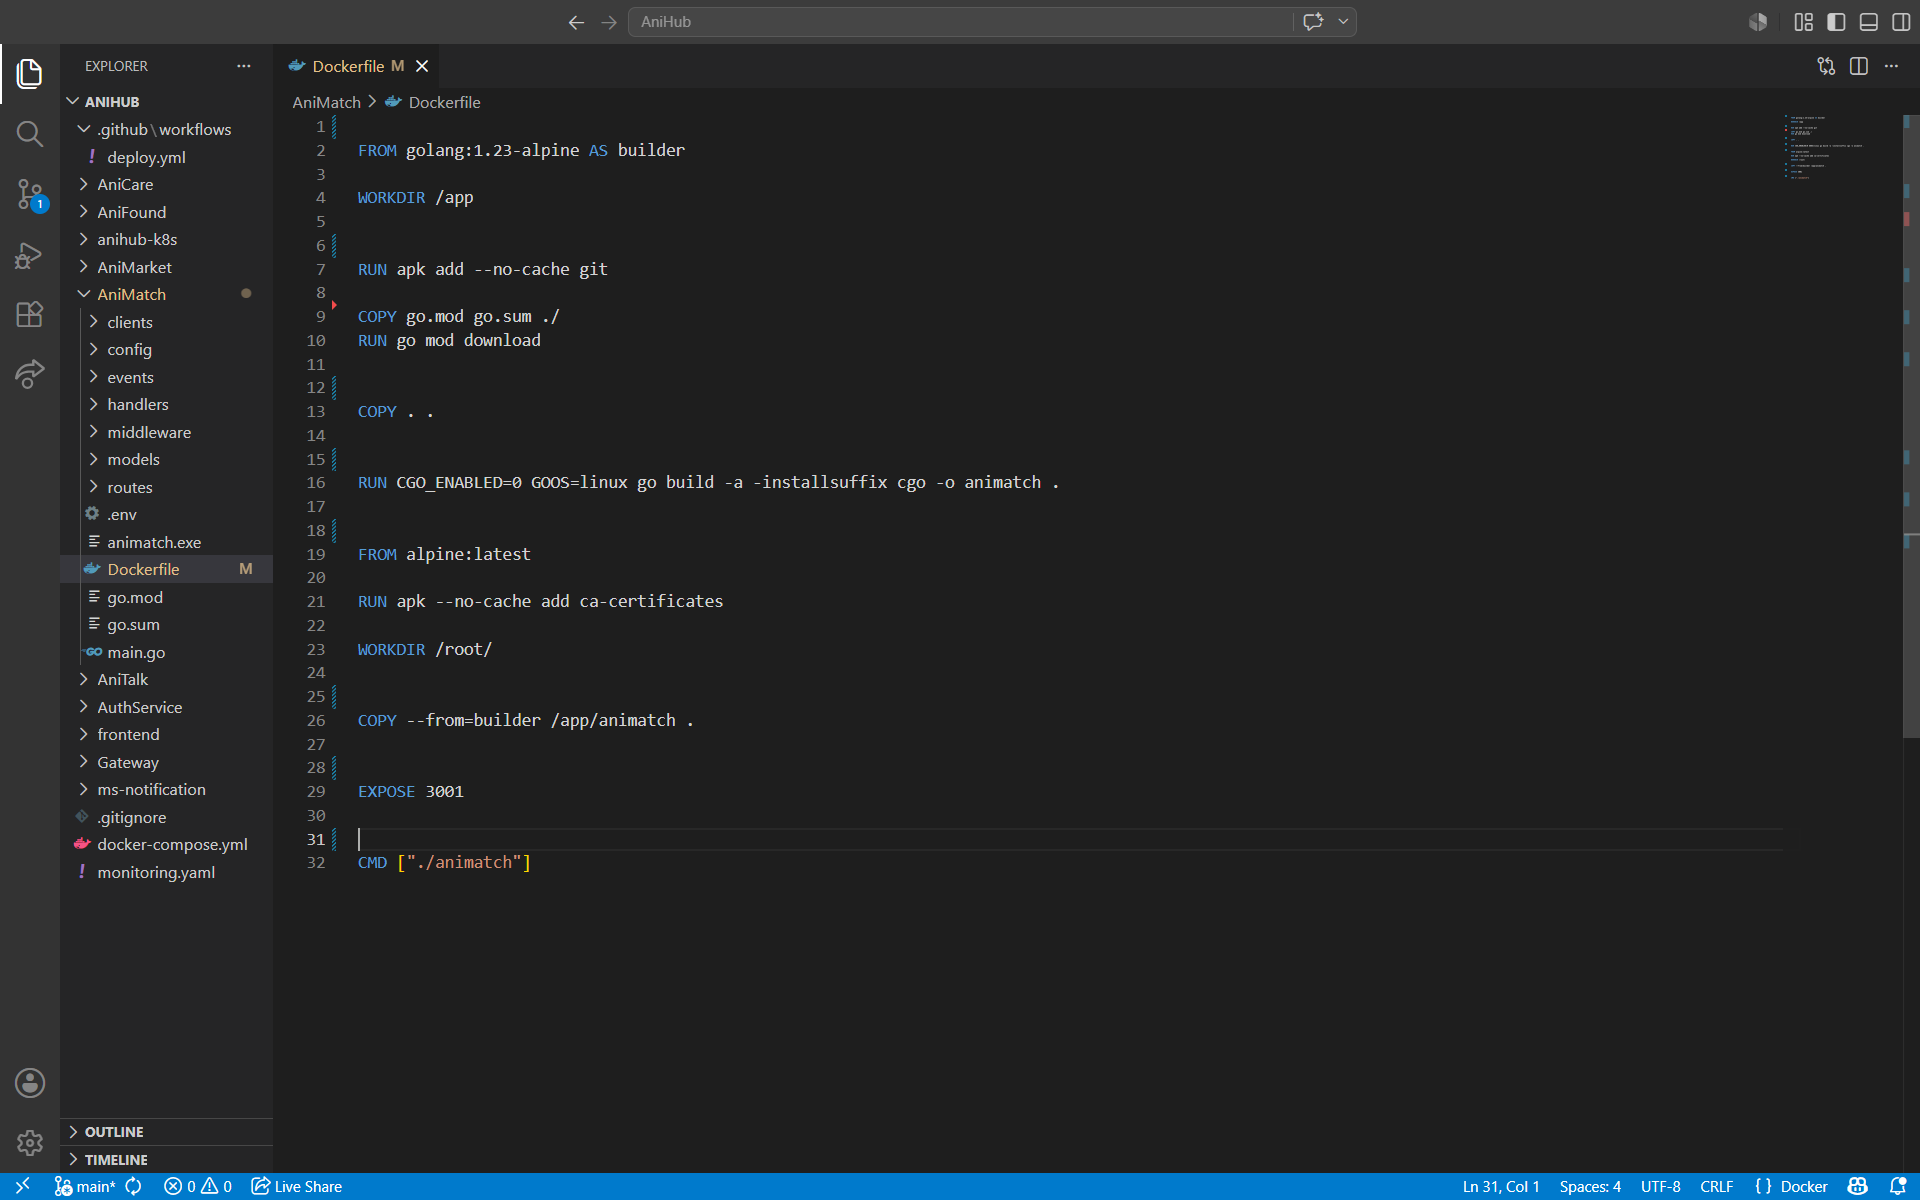
\includegraphics[width=0.65\linewidth]{images/dokcer file.png}
    \caption{Exemple de fichier Dockerfile du microservice \textit{AniMatch}}
    \label{fig:dockerfile-animatch}
\end{figure}

 \newpage
\subsubsection{Configuration de Docker Compose}

Cette figure illustre notre fichier \textit{docker-compose.yml}, utilisé pour orchestrer et exécuter l’ensemble des microservices ainsi que leurs dépendances dans des conteneurs Docker : 

\begin{figure}[H]
    \centering
    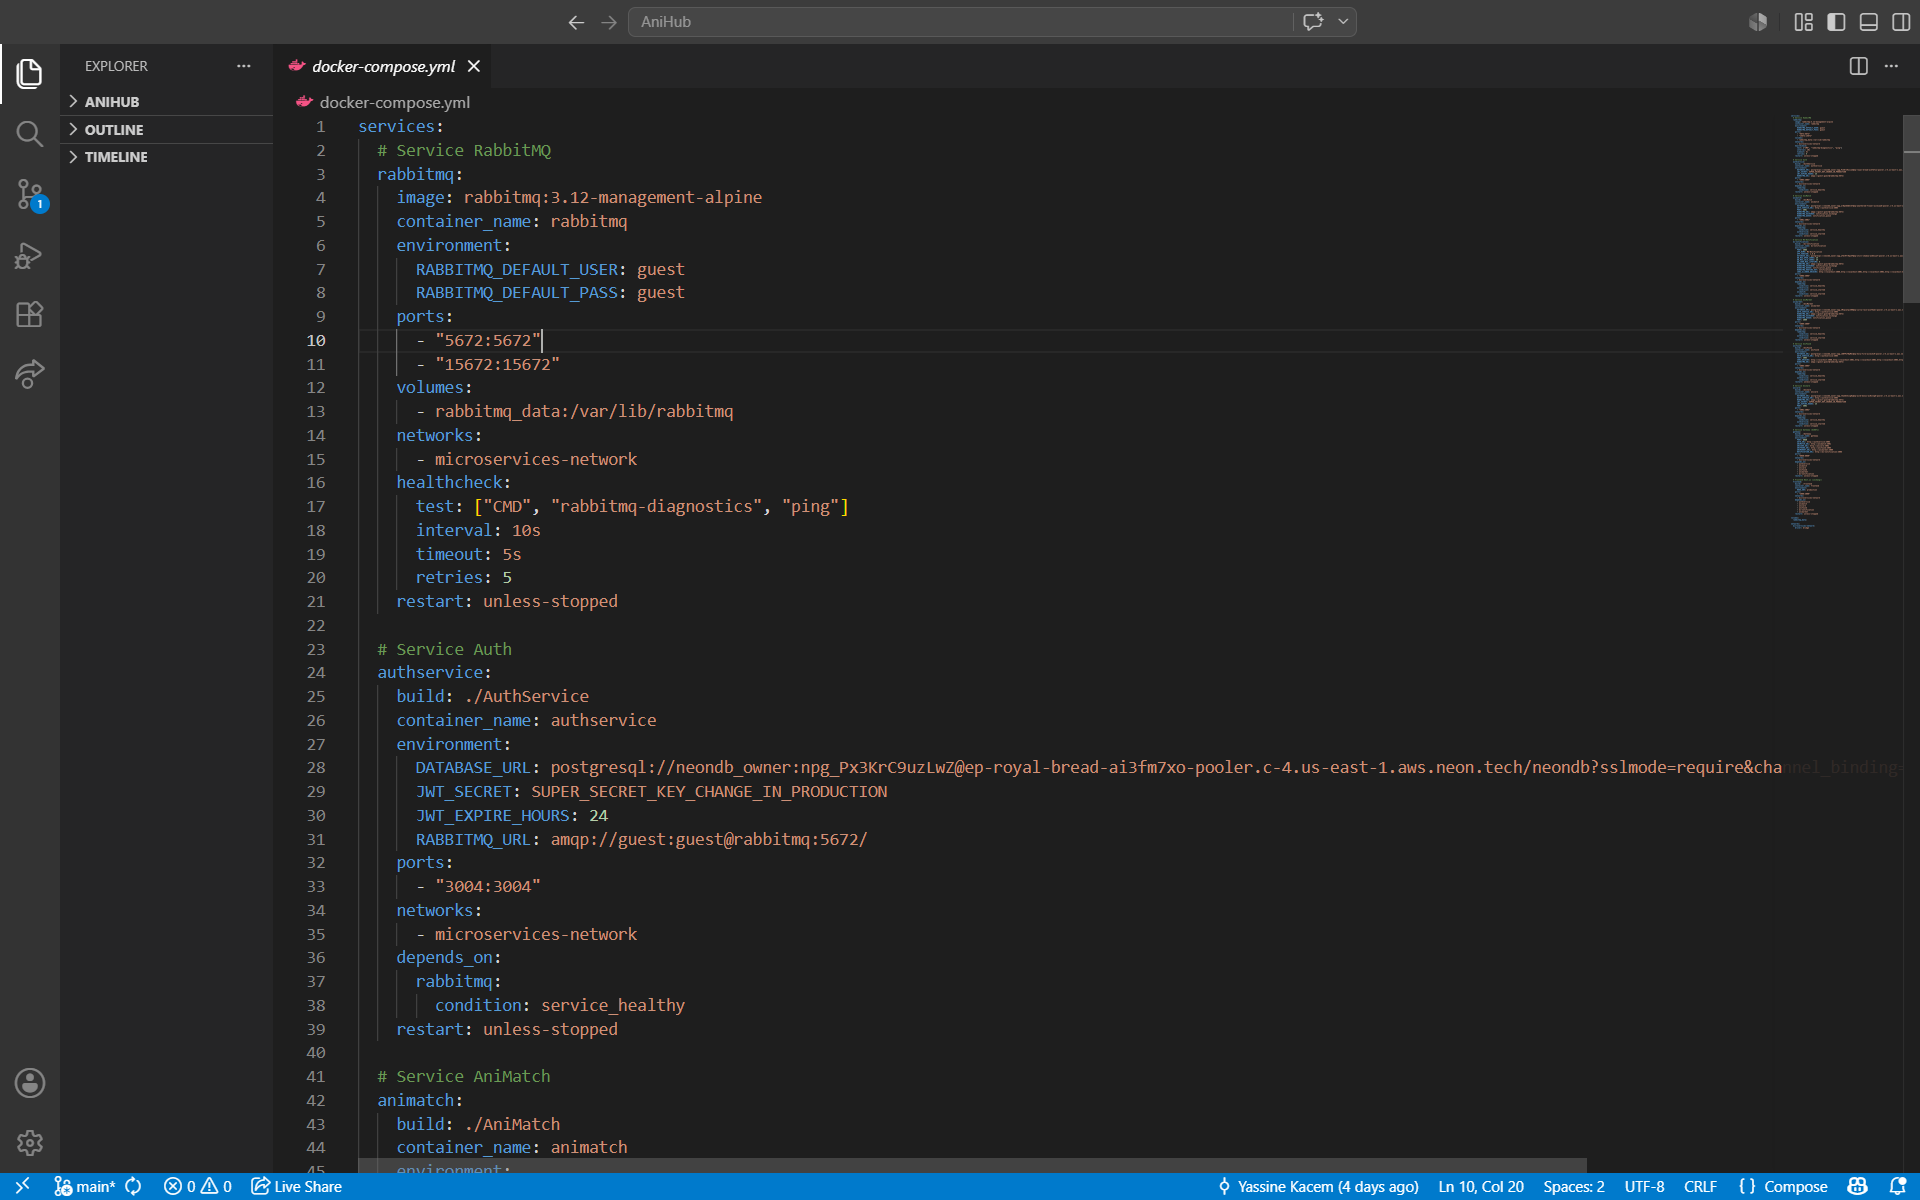
\includegraphics[width=0.75\linewidth]{images/docker compose.png}
    \caption{Configuration du fichier Docker Compose}
    \label{fig:docker-compose}
\end{figure}  
\subsubsection{Construction et exécution des conteneurs} 
Ces figures présentent les différentes étapes de construction et de lancement des conteneurs de l’application.
\begin{figure}[h!]
    \centering
    
    \begin{minipage}{0.48\textwidth}
        \centering
        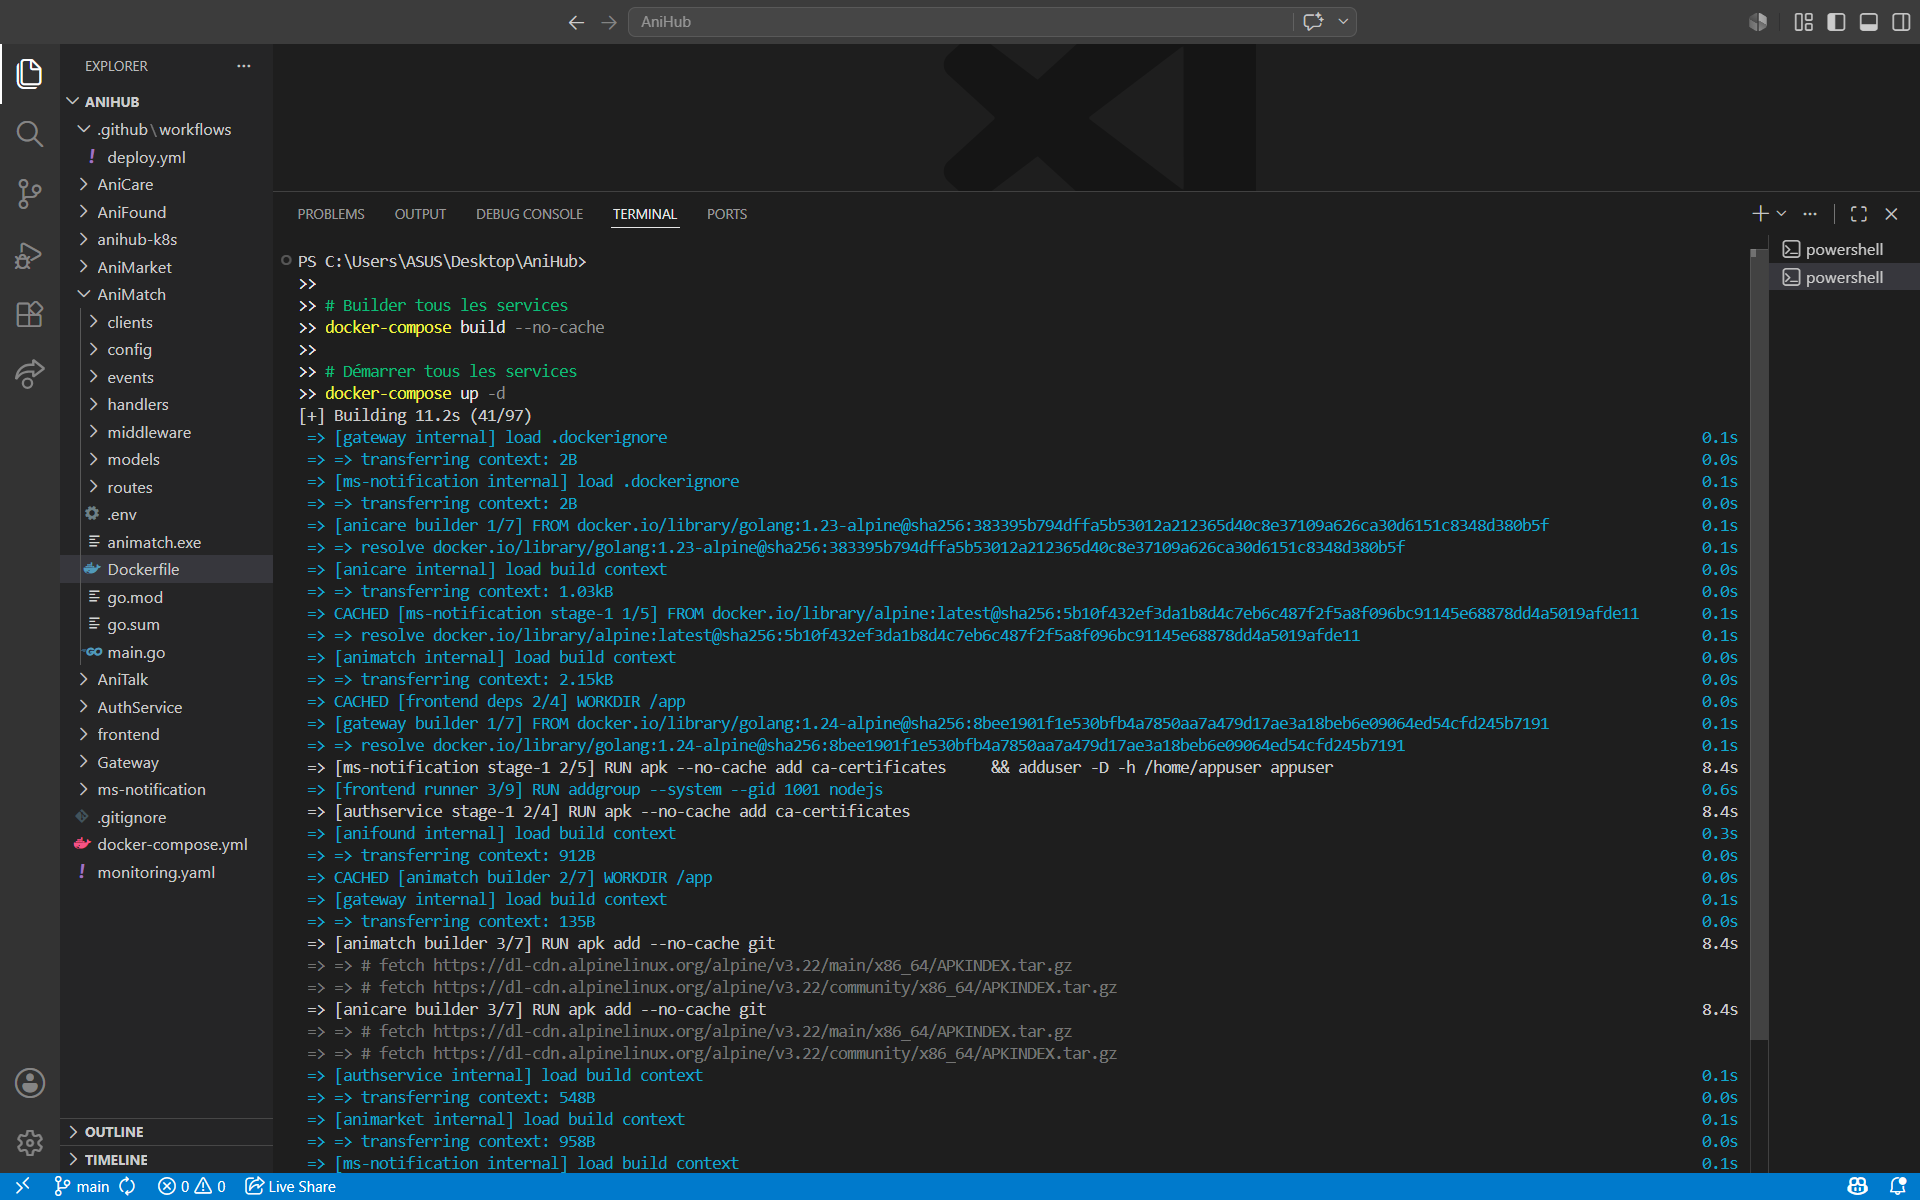
\includegraphics[width=\textwidth,height=5.6cm]{images/creation des conteneurs.png}
        \caption{Construction et démarrage des conteneurs}
    \end{minipage}
    \hfill
    \begin{minipage}{0.48\textwidth}
        \centering
        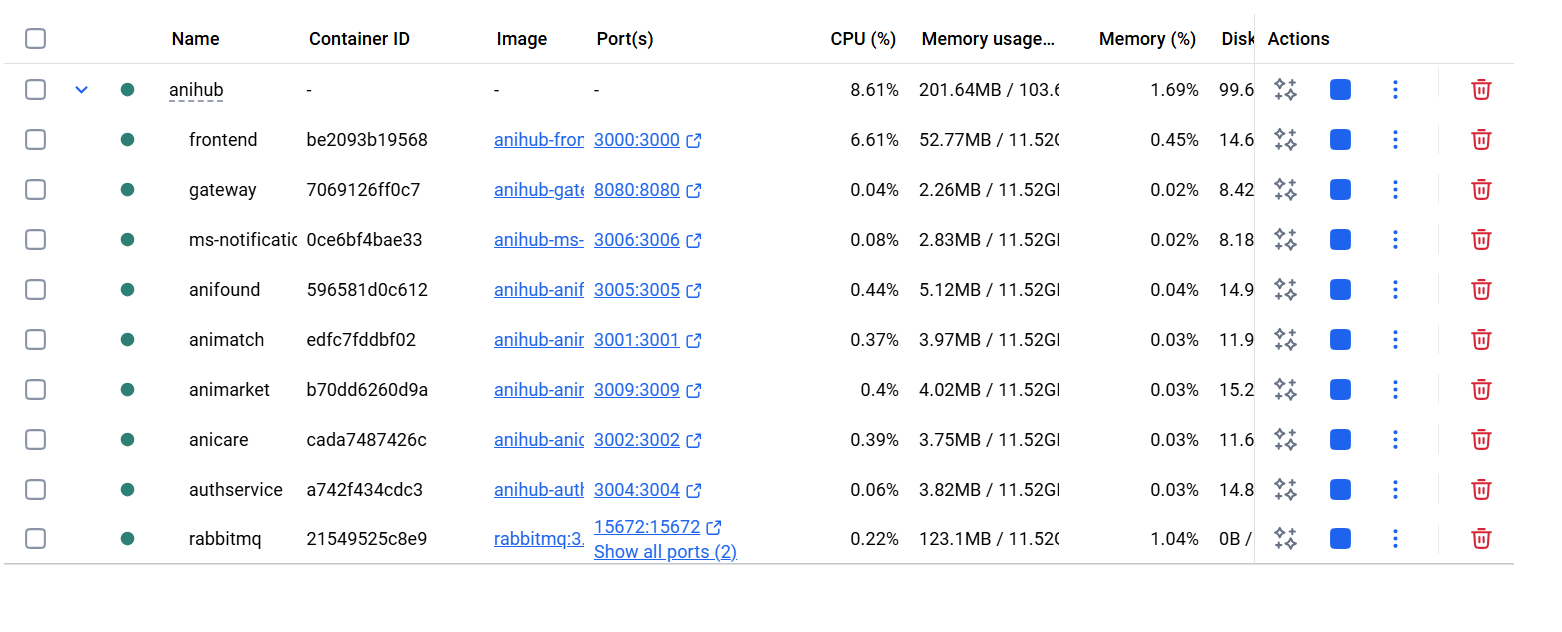
\includegraphics[width=\textwidth,height=5.6cm]{images/execution des conteneurs.png}
        \caption{Conteneurs Docker en cours d’exécution}
    \end{minipage}

\end{figure}
 \newpage
\subsection{Déploiement des microservices avec Kubernetes}  
\subsubsection{Création des fichiers Deployment et Service}

Cette figure illustre le fichier \textit{deployment-anifound.yaml}, utilisé pour définir et déployer le microservice \textit{AniFound} dans l’environnement Kubernetes.

\begin{figure}[H]
    \centering
    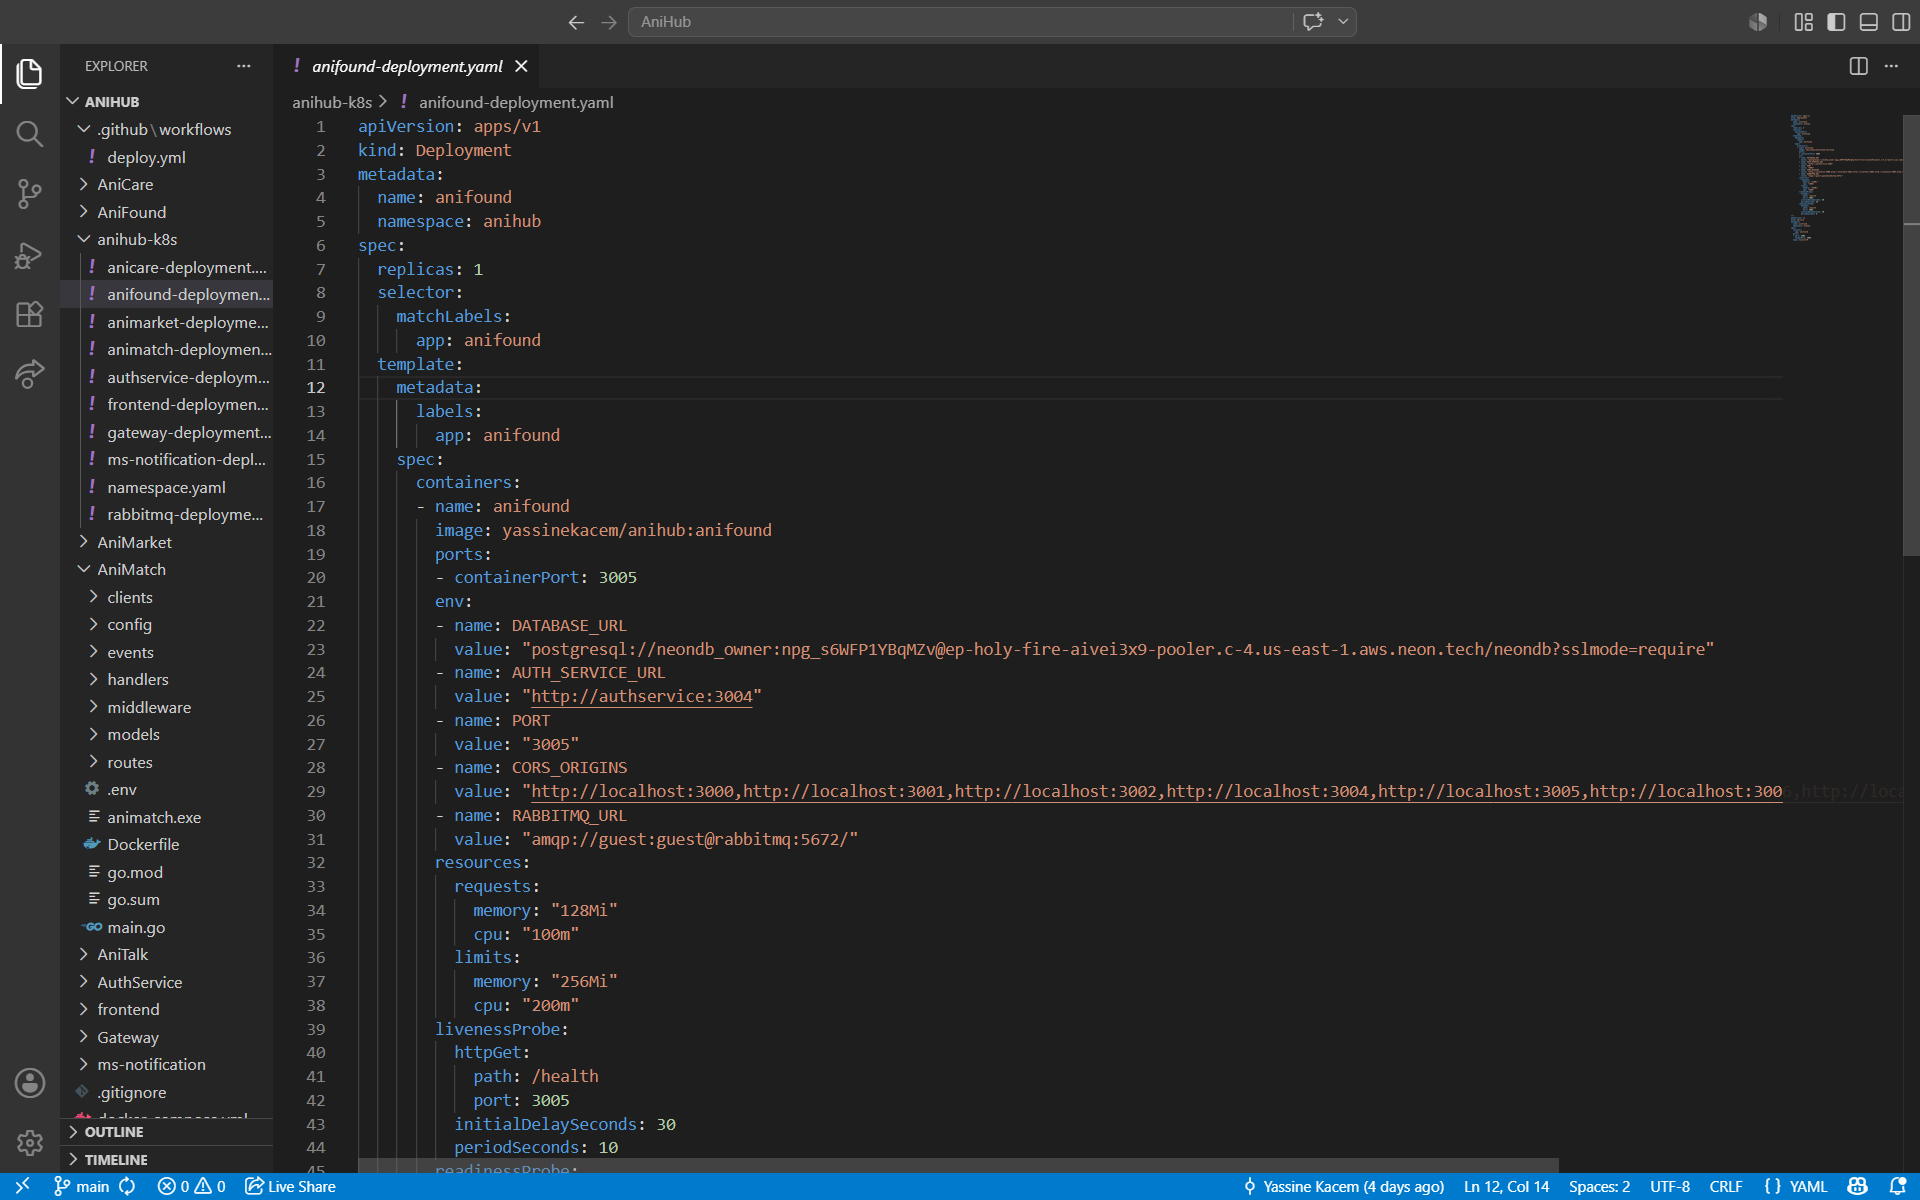
\includegraphics[width=0.7\linewidth]{images/deploymentservice k8s.png}
    \caption{Fichier Deployment du microservice \textit{AniFound}}
    \label{fig:deployment-anifound}
\end{figure}   

\subsubsection{Application des fichiers YAML dans Kubernetes pour le déploiement d’AniHub} 
Cette figure illustre l’application des fichiers de configuration YAML dans Kubernetes pour déployer les microservices d’AniHub : 
\begin{figure}[H]
    \centering
    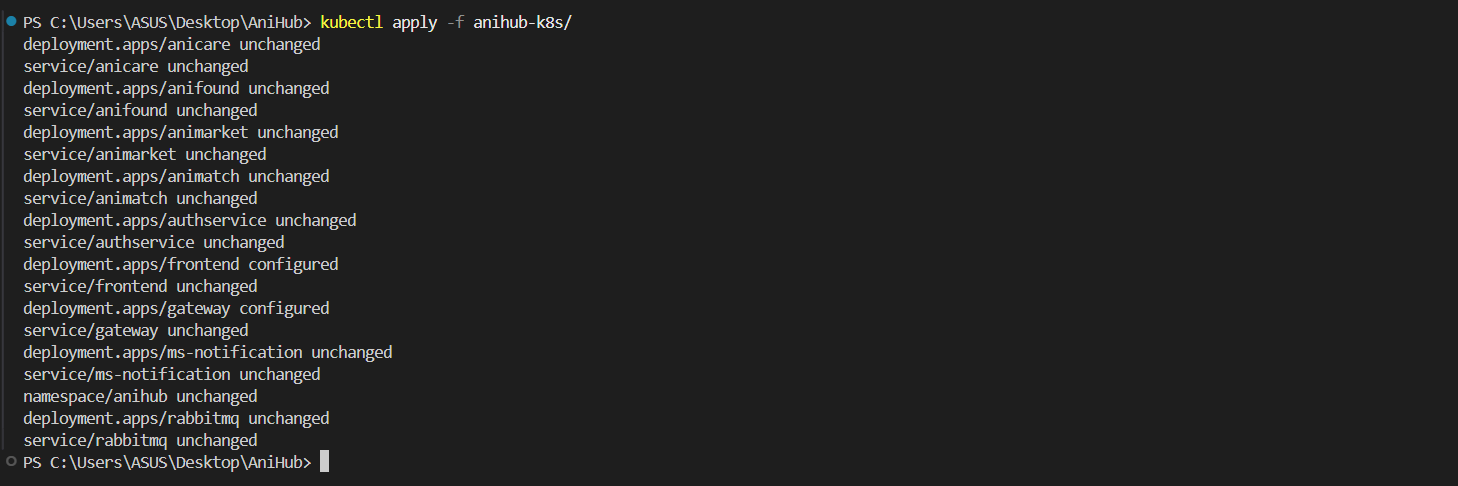
\includegraphics[width=0.9\linewidth]{images/apply files k8s.png}
    \caption{Application des fichiers YAML dans Kubernetes pour le déploiement d’AniHub}
    \label{fig:deploiement-k8s} 
\end{figure}
\newpage 
\subsubsection{Vérification de l’état des pods}  

Cette figure illustre l’état des pods déployés sur Kubernetes afin de vérifier le bon fonctionnement des différents microservices de l’application AniHub : 
\begin{figure}[H]
    \centering
    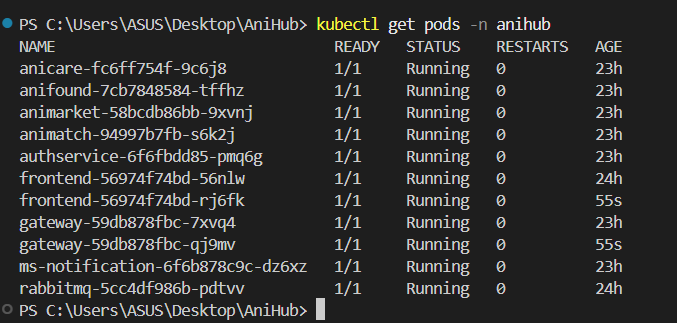
\includegraphics[width=0.56\linewidth]{images/get pods.png}
    \caption{Vérification de l’état des pods sur Kubernetes}
    \label{fig:pods-k8s}
\end{figure} 

\subsubsection{Exécution des conteneurs via Kubernetes}

Cette figure illustre l’exécution des conteneurs de l’application AniHub dans Docker Desktop, orchestrés par Kubernetes avec un nombre de replicas égal à 1 pour chaque microservice : 
\begin{figure}[H]
    \centering
    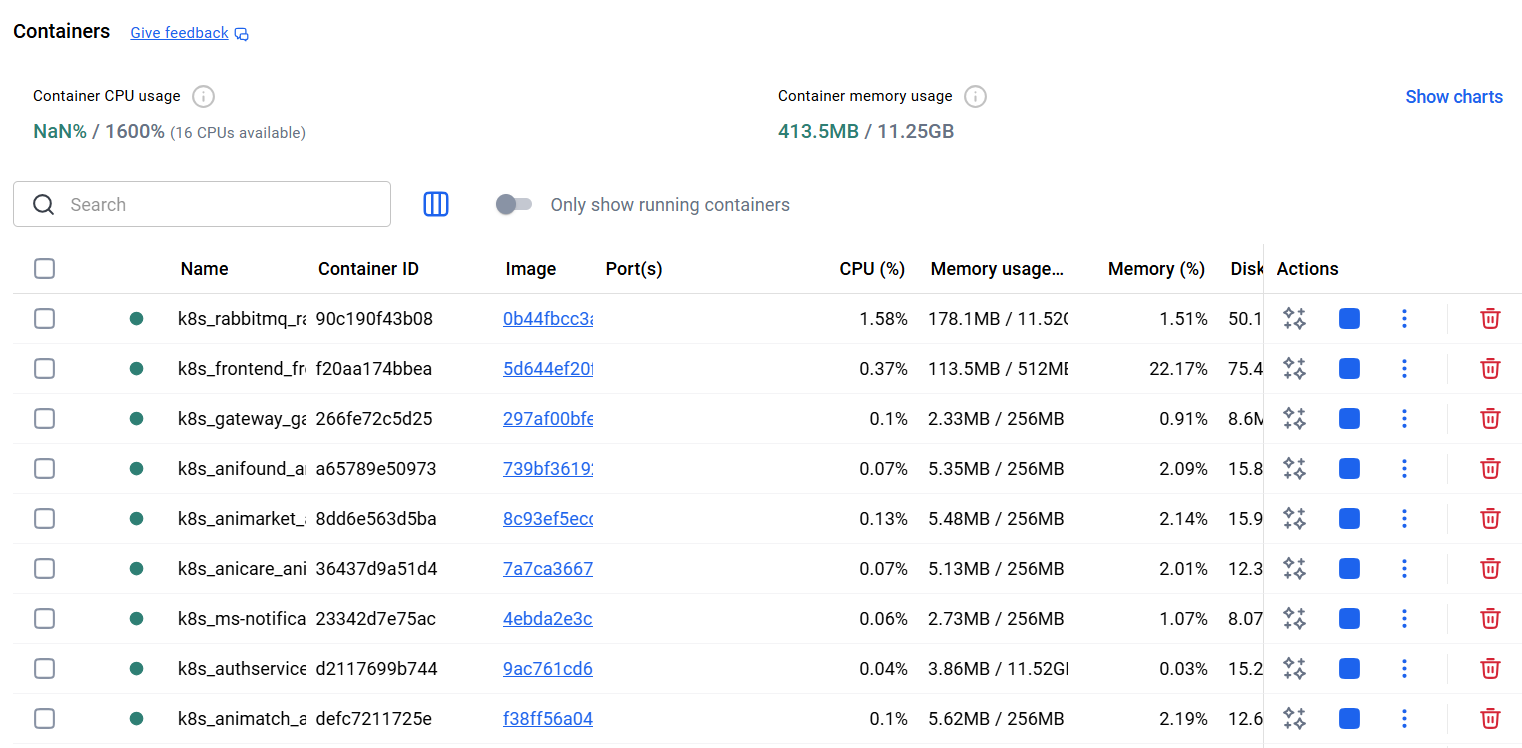
\includegraphics[width=0.56\linewidth]{images/conatiner run from k8s.png}
    \caption{Exécution des conteneurs de l’application AniHub via Kubernetes}
    \label{fig:containers-k8s}
\end{figure} 
\subsubsection{Accès au frontend via port-forward sur le port 3000}
Cette figure illustre l’accès à l’interface frontend de l’application AniHub via un port-forward Kubernetes sur le port 3000, afin de tester l’application en local après le déploiement : 
\begin{figure}[H]
    \centering
    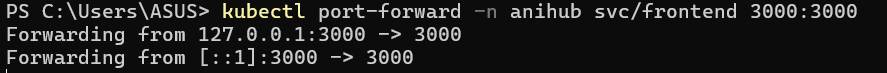
\includegraphics[width=0.66\linewidth]{images/forward.png}
    \caption{Accès au frontend via port-forward sur le port 3000}
    \label{fig:port-forward}
\end{figure} 
\newpage
\subsection{Déploiement Cloud sur Google Cloud Platform} 


\subsubsection{Vérification du contexte cloud}

Cette étape consiste à vérifier que le contexte Kubernetes est bien configuré sur le cluster cloud d’AniHub. Elle permet de s’assurer que les commandes kubectl sont exécutées sur le bon cluster GCP et que l’environnement cible est correctement sélectionné avant le déploiement ou les tests : 

\begin{figure}[H]
    \centering
    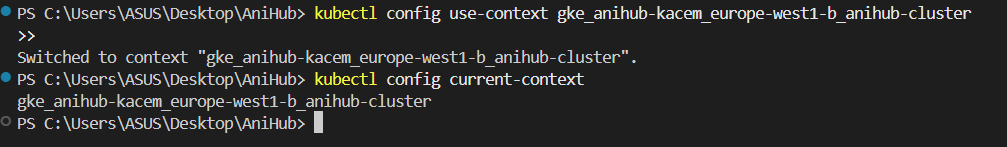
\includegraphics[width=0.76\linewidth]{images/verifons context cloud 1.png}
    \caption{Vérification du contexte Kubernetes sur le cluster cloud de GCP}
    \label{fig:context-cloud}
\end{figure} 

\subsubsection{Affichage des clusters disponibles sur GCP}
Cette figure illustre la liste des clusters Kubernetes disponibles sur Google Cloud Platform (GCP) afin de confirmer que le cluster destiné au déploiement d’AniHub est bien présent et accessible : 
\begin{figure}[H]
    \centering
    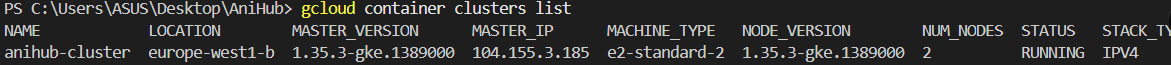
\includegraphics[width=0.96\linewidth]{images/Voir les clusters GCP disponibles 2.png}
    \caption{Affichage des clusters Kubernetes disponibles sur GCP}
    \label{fig:clusters-gcp}
\end{figure}  

\subsubsection{État des pods dans le cluster AniHub sur GCP} 
Cette figure illustre l’état des pods déployés dans le cluster Kubernetes d’AniHub sur Google Cloud Platform (GCP) afin de vérifier que les microservices sont correctement déployés et en cours d’exécution : 
\begin{figure}[H]
    \centering
    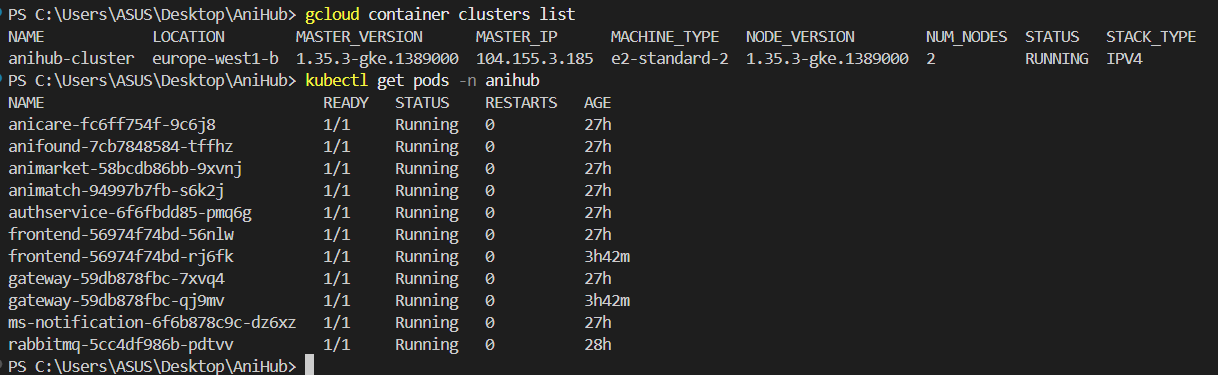
\includegraphics[width=0.76\linewidth]{images/etat des pods dans le cluster.png}
    \caption{État des pods dans le cluster AniHub sur GCP}
    \label{fig:pods-gcp}
\end{figure} 

\newpage  
\subsubsection{Accès cloud et tests de communication entre les microservices } 
Cette figure illustre l’accès à l’application déployée sur le cloud ainsi que les tests de communication entre les microservices frontend et authservice : 
\begin{figure}[H]
    \centering
    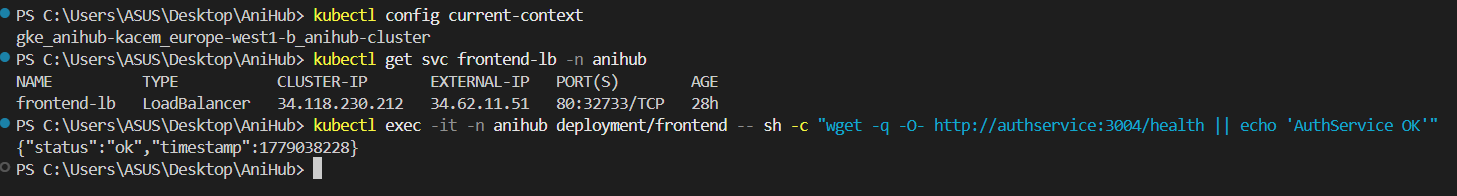
\includegraphics[width=0.76\linewidth]{images/Accès cloud et tests de communication entre microservices.png}
    \caption{Accès cloud et tests de communication entre les microservices}
    \label{fig:communication-microservices}
\end{figure}

\subsubsection{Liste des services Kubernetes et accès à l’application via l’IP externe} 
Cette figure illustre la liste des services Kubernetes ainsi que l’accès à l’application déployée sur le cloud via l’IP externe : 
\begin{figure}[H]
    \centering
    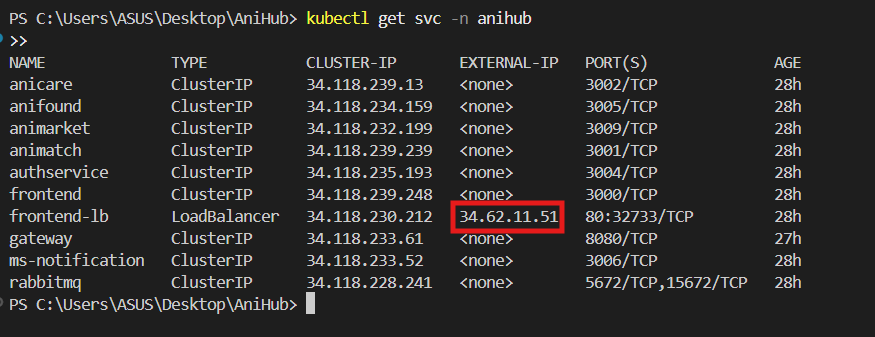
\includegraphics[width=0.62\linewidth]{images/Liste des services Kubernetes et accès à l’application via l’IP externe 4.png}
    \caption{Liste des services Kubernetes et accès à l’application via l’IP externe}
    \label{fig:services-k8s}
\end{figure} 

\subsubsection{Test de l’application déployée via l’IP externe 34.62.11.51 sur le navigateur} 
Cette figure illustre le test de l’application AniHub déployée sur le cloud via l’IP externe : 
\begin{figure}[H]
    \centering
    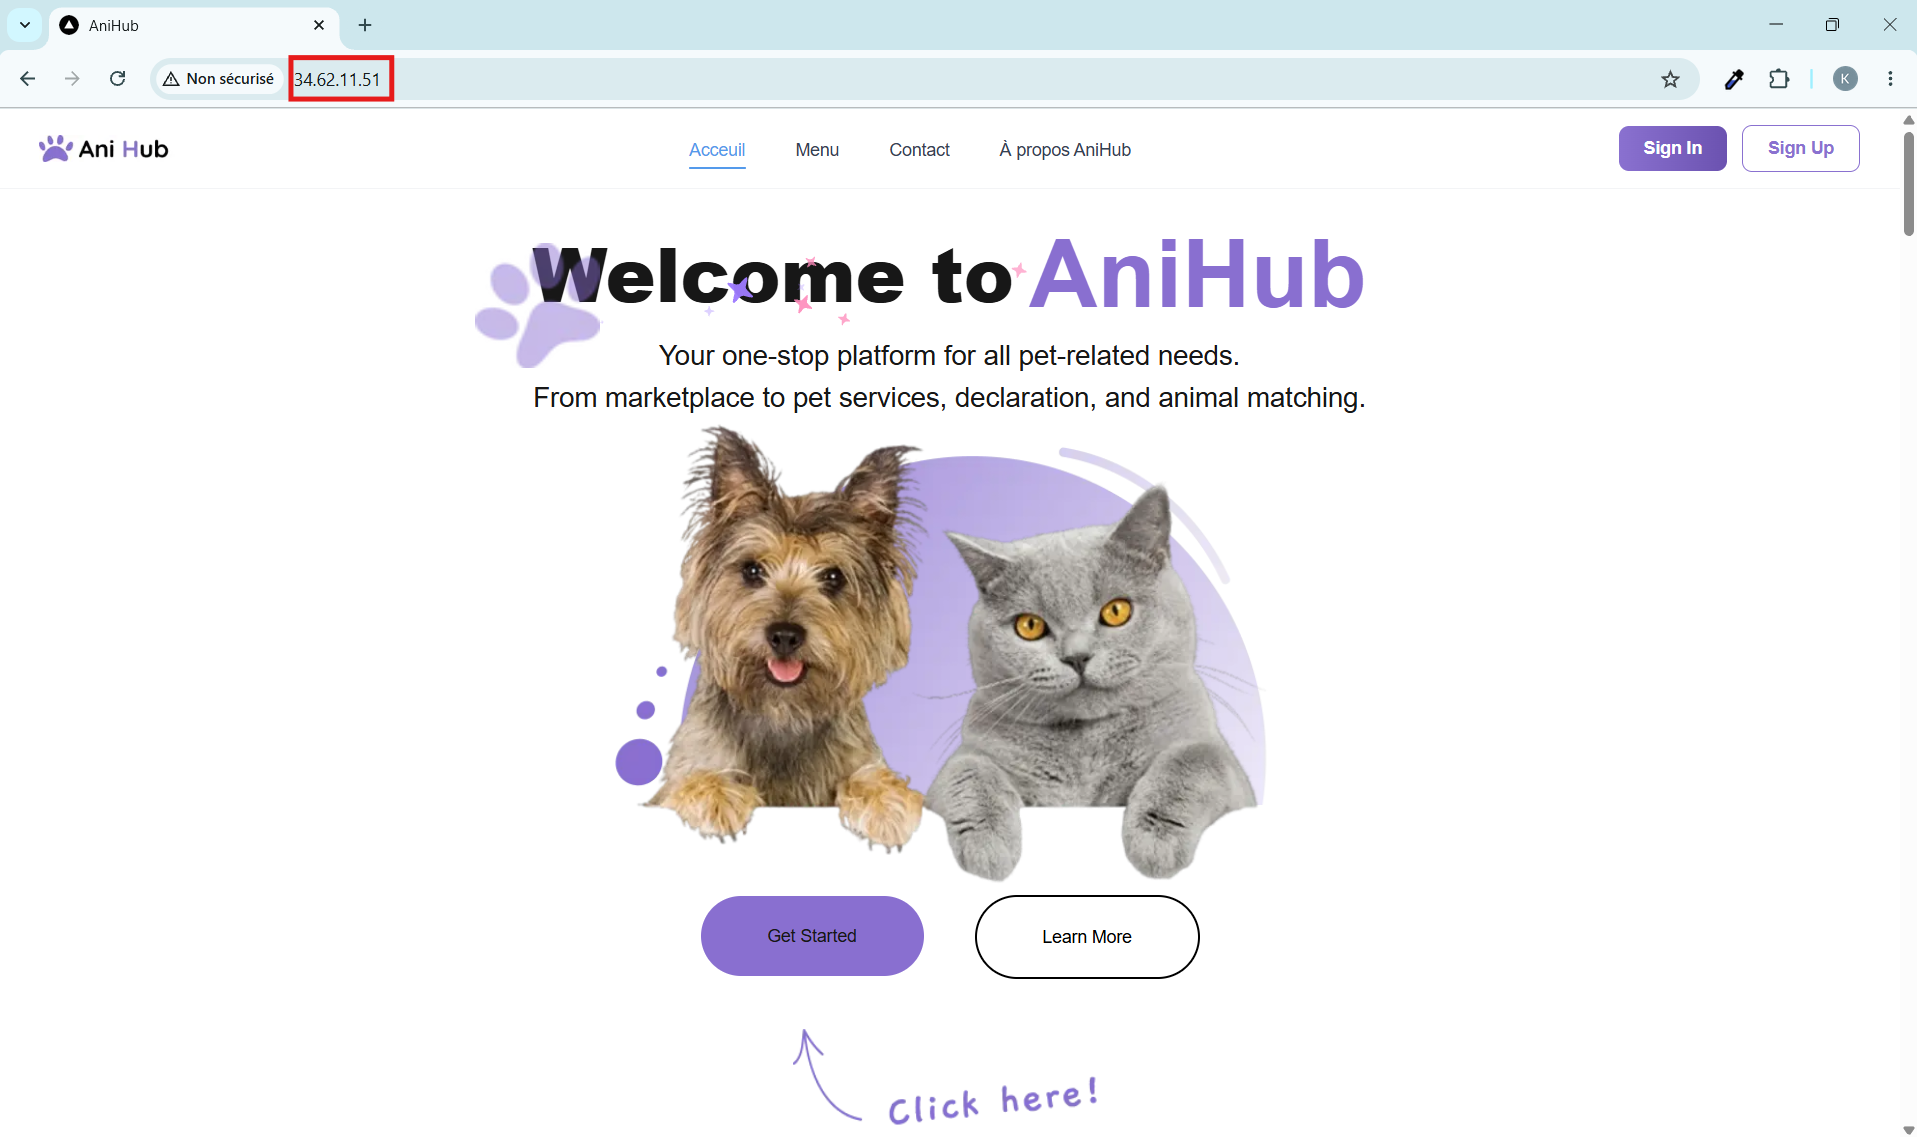
\includegraphics[width=0.72\linewidth]{images/app deployé sur cloud 6.png}
    \caption{Test de l’application déployée via l’IP externe sur le navigateur}
    \label{fig:test-application-cloud}
\end{figure} 
\newpage

\subsection{Mise en place du pipeline CI/CD} 
\subsubsection{Création du workflow GitHub Actions}

Cette figure illustre le fichier \textbf{.github/workflow/deploy.yml} qui définit les étapes nécessaires de la pipeline CI/CD, à savoir :

\begin{itemize}
    \item Authentification à Docker Hub
    \item Construction des images Docker des microservices
    \item Scan et validation des images Docker
    \item Publication des images sur Docker Hub
    \item Authentification à Google Cloud Platform (GCP)
    \item Configuration du SDK Google Cloud
    \item Récupération des identifiants du cluster Kubernetes (GKE)
    \item Déploiement des microservices sur Kubernetes
    \item Redémarrage des déploiements Kubernetes
    \item Attente de la disponibilité des services
    \item Vérification du statut du déploiement
\end{itemize}  

\begin{figure}[H]
    \centering
    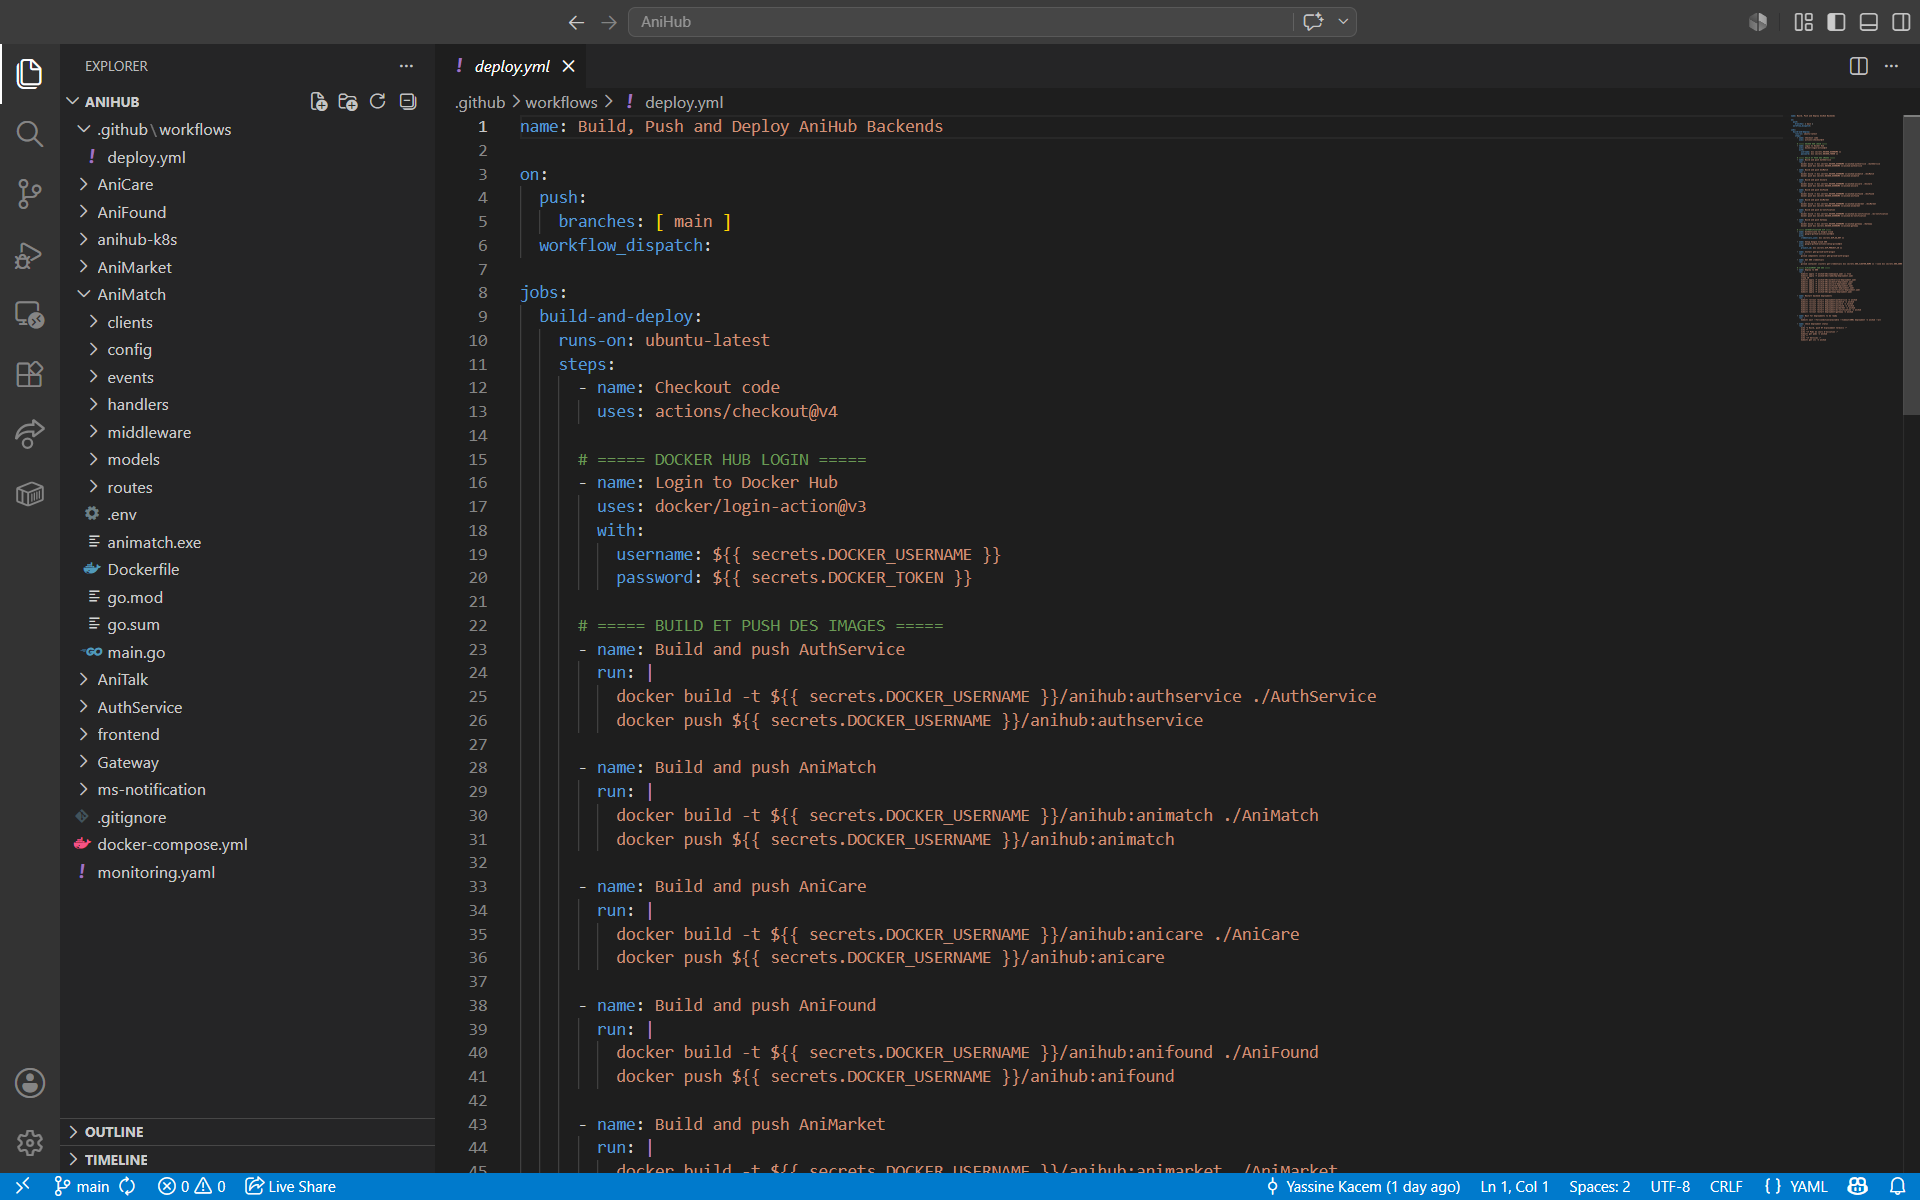
\includegraphics[width=0.68\linewidth]{images/pipeline1.png}
    \caption{Fichier de workflow GitHub Actions pour la pipeline CI/CD}
    \label{fig:workflow-ci-cd}
\end{figure}

\subsubsection{Déclenchement de la pipeline CI/CD par un push sur GitHub} 
Cette figure illustre un push vers le dépôt GitHub permettant de déclencher automatiquement la pipeline CI/CD : 
\begin{figure}[H]
    \centering
    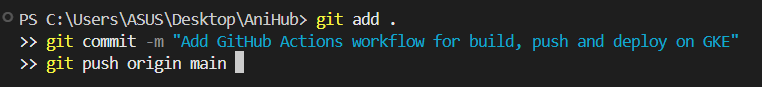
\includegraphics[width=0.55\linewidth]{images/declenche pipeline.png}
    \caption{Déclenchement de la pipeline CI/CD par un push sur GitHub}
    \label{fig:trigger-ci-cd} 
\end{figure}    

\newpage
\subsubsection{Exécution de la pipeline dans GitHub Actions} 
Cette figure illustre l’exécution de la pipeline CI/CD dans GitHub Actions après un push sur le dépôt GitHub : 
\begin{figure}[H]
    \centering
    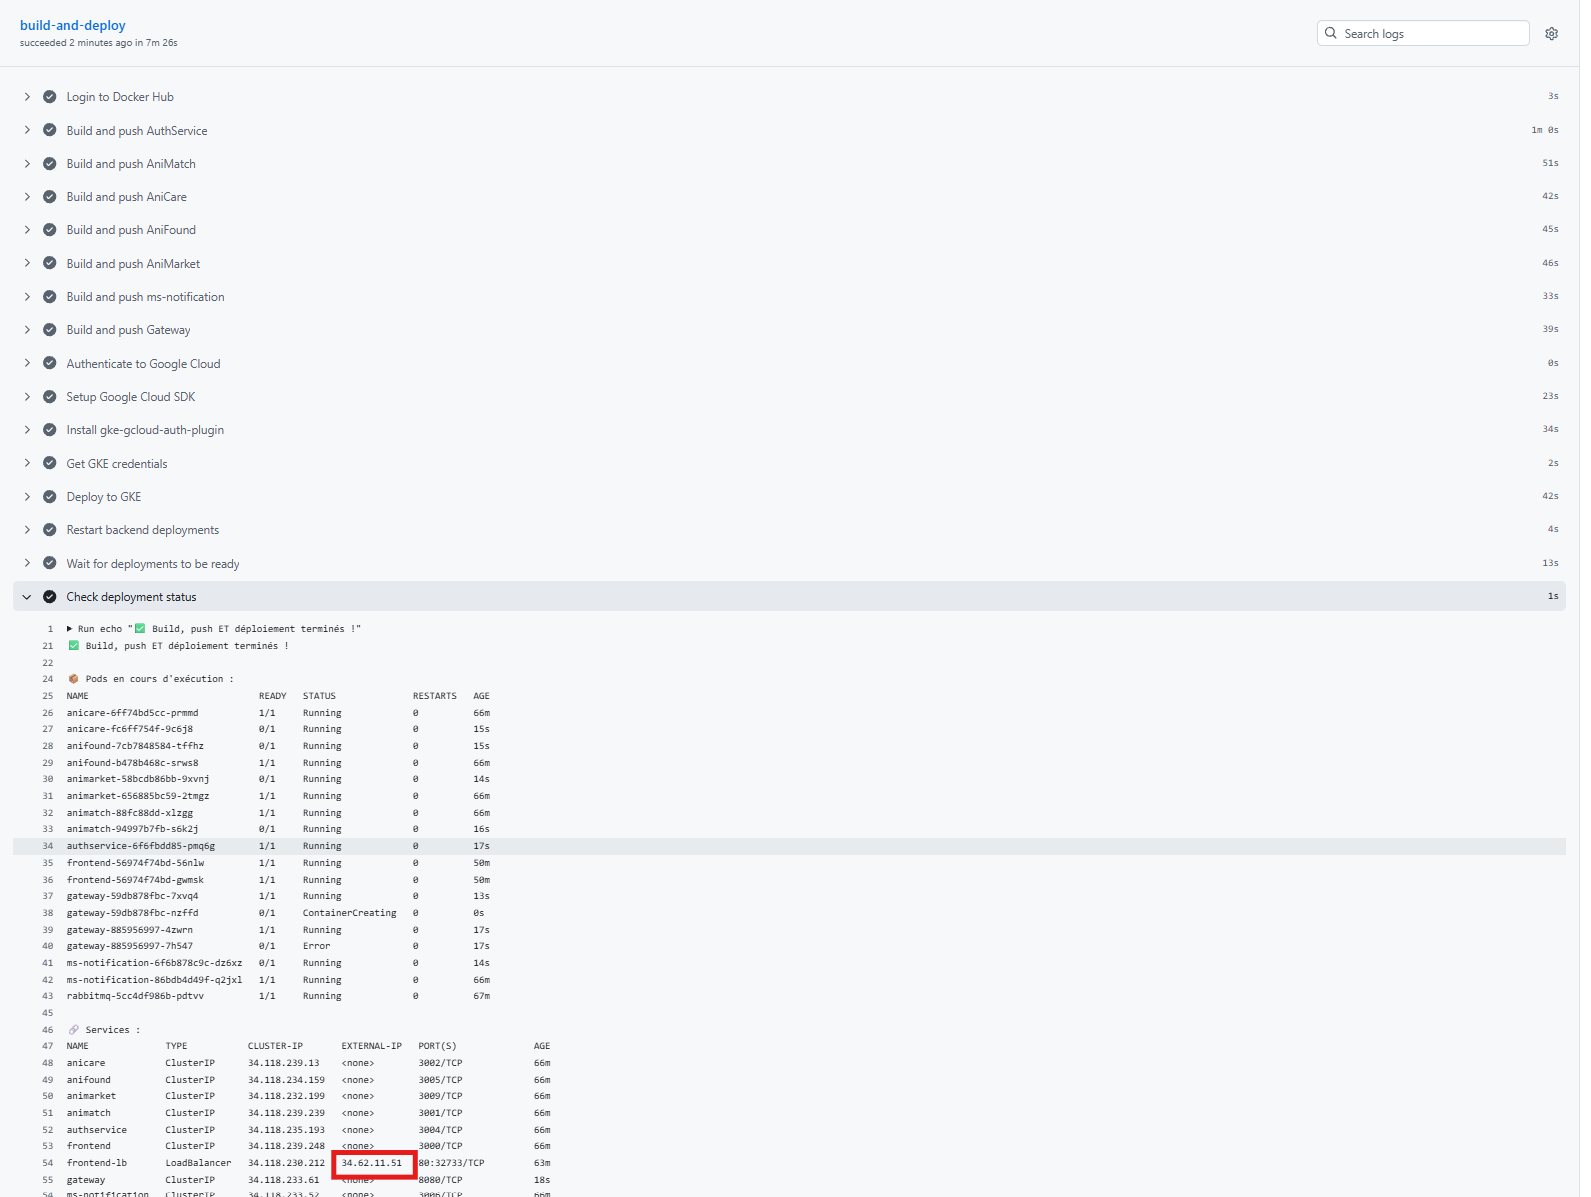
\includegraphics[width=1.3\linewidth]{images/pipeline2.png}
    \caption{Exécution de la pipeline CI/CD dans GitHub Actions}
    \label{fig:execution-ci-cd}
\end{figure} 

\newpage 
\subsection{Monitoring et supervision} 
\subsubsection{Configuration de Prometheus et Grafana sur Kubernetes}

Cette figure illustre le fichier \textbf{monitoring.yml} utilisé pour déployer et configurer Prometheus et Grafana sur Kubernetes afin d’assurer le monitoring des microservices d’AniHub : 
\begin{figure}[H]
    \centering
    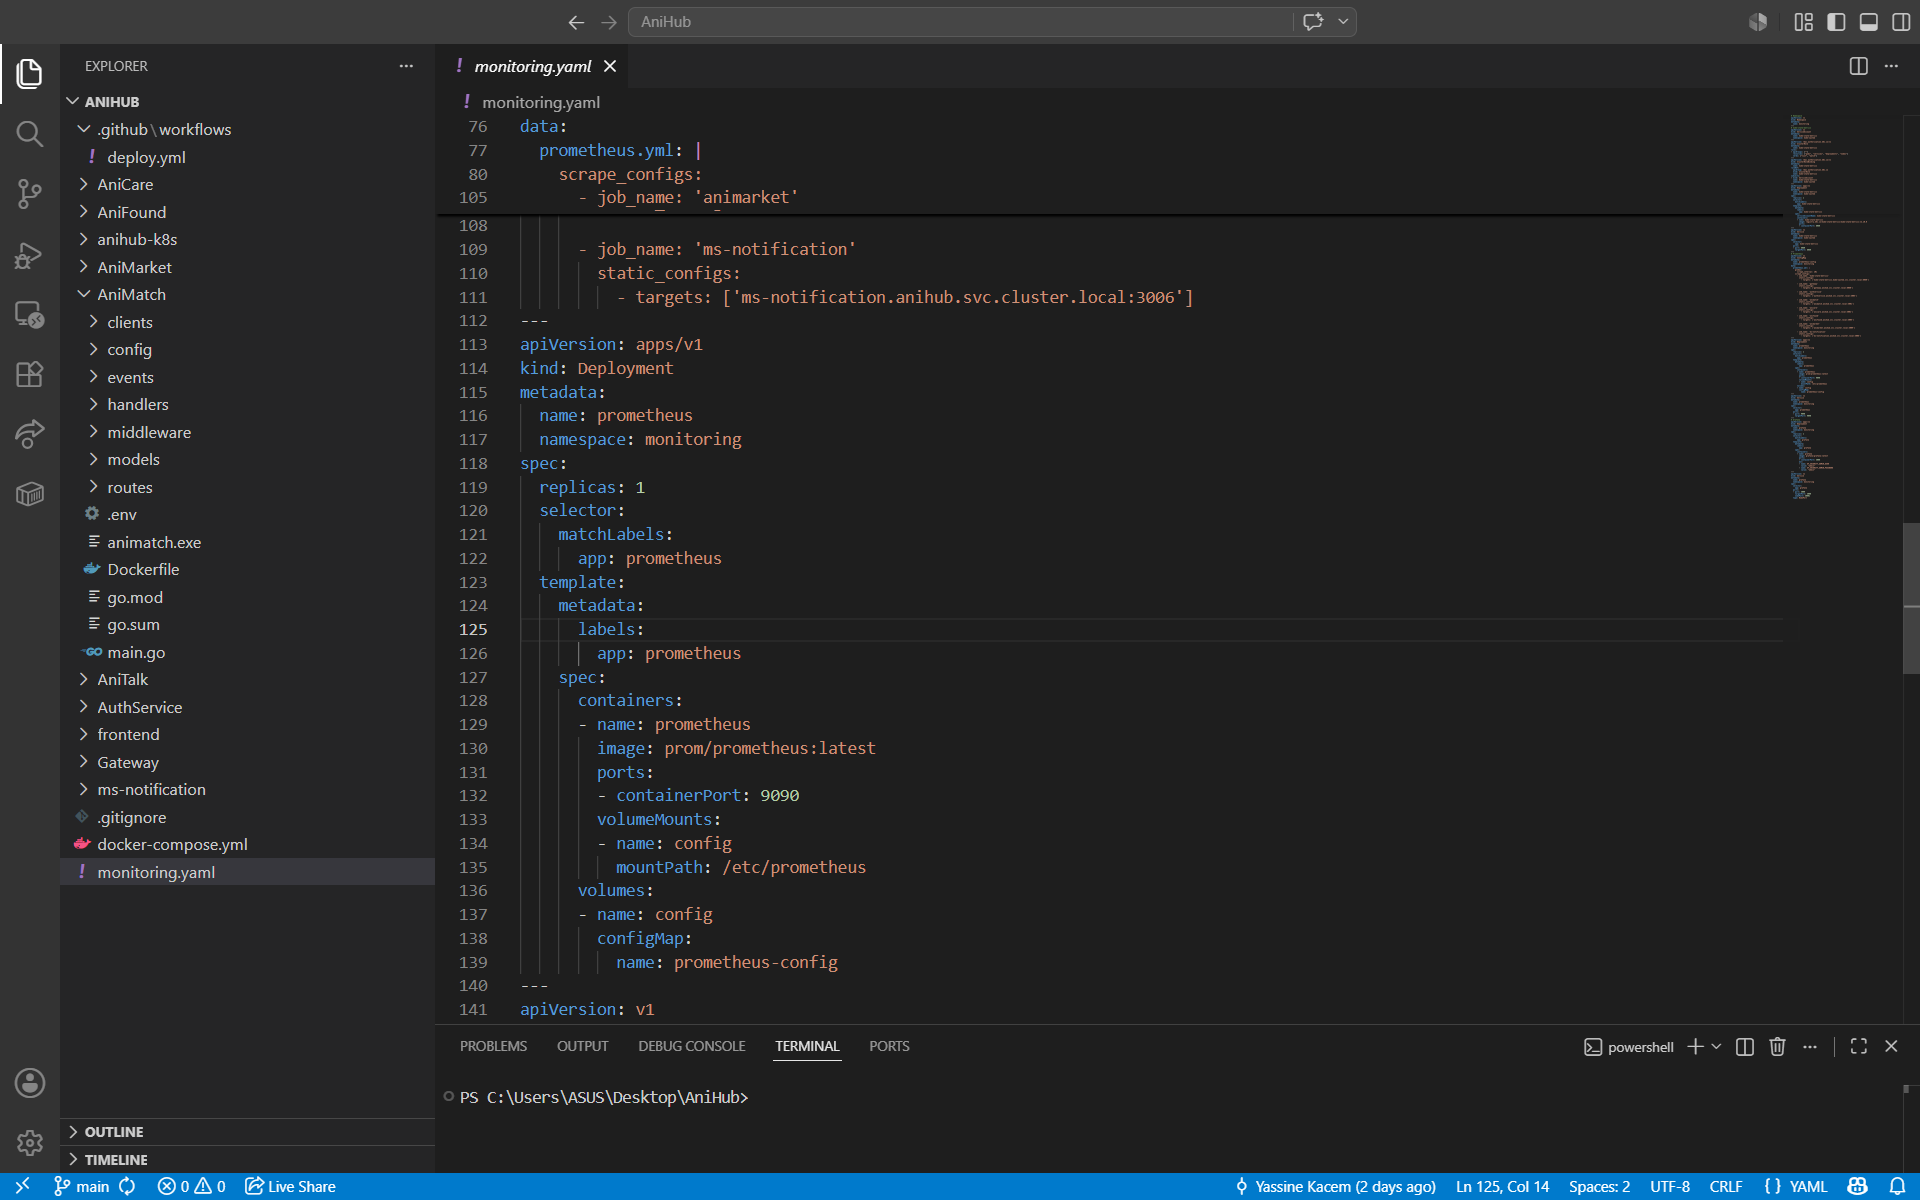
\includegraphics[width=0.4\linewidth]{images/monitoring.yaml.png}
    \caption{Configuration de Prometheus et Grafana sur Kubernetes}
    \label{fig:monitoring-k8s}
\end{figure}  

\subsubsection{Ajout de la route des métriques dans les microservices}

Cette étape permet à Prometheus de collecter les métriques des microservices via la route \texttt{/metrics} afin d’assurer le monitoring de l’application. 
\begin{figure}[H]
    \centering
    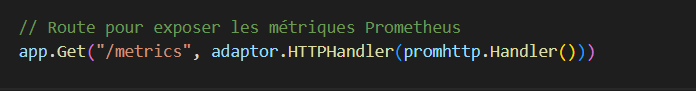
\includegraphics[width=0.6\linewidth]{images/route metric.png}
    \caption{Ajout de la route des métriques dans les microservices}
    \label{fig:metrics-route}
\end{figure} 

\subsubsection{Surveillance des microservices avec Prometheus} 


Cette figure illustre la surveillance des microservices par Prometheus via les targets configurées. Par exemple, le microservice \textbf{gateway} est en état \textbf{UP}, confirmant son bon fonctionnement et la collecte des métriques : 
\begin{figure}[H]
    \centering
    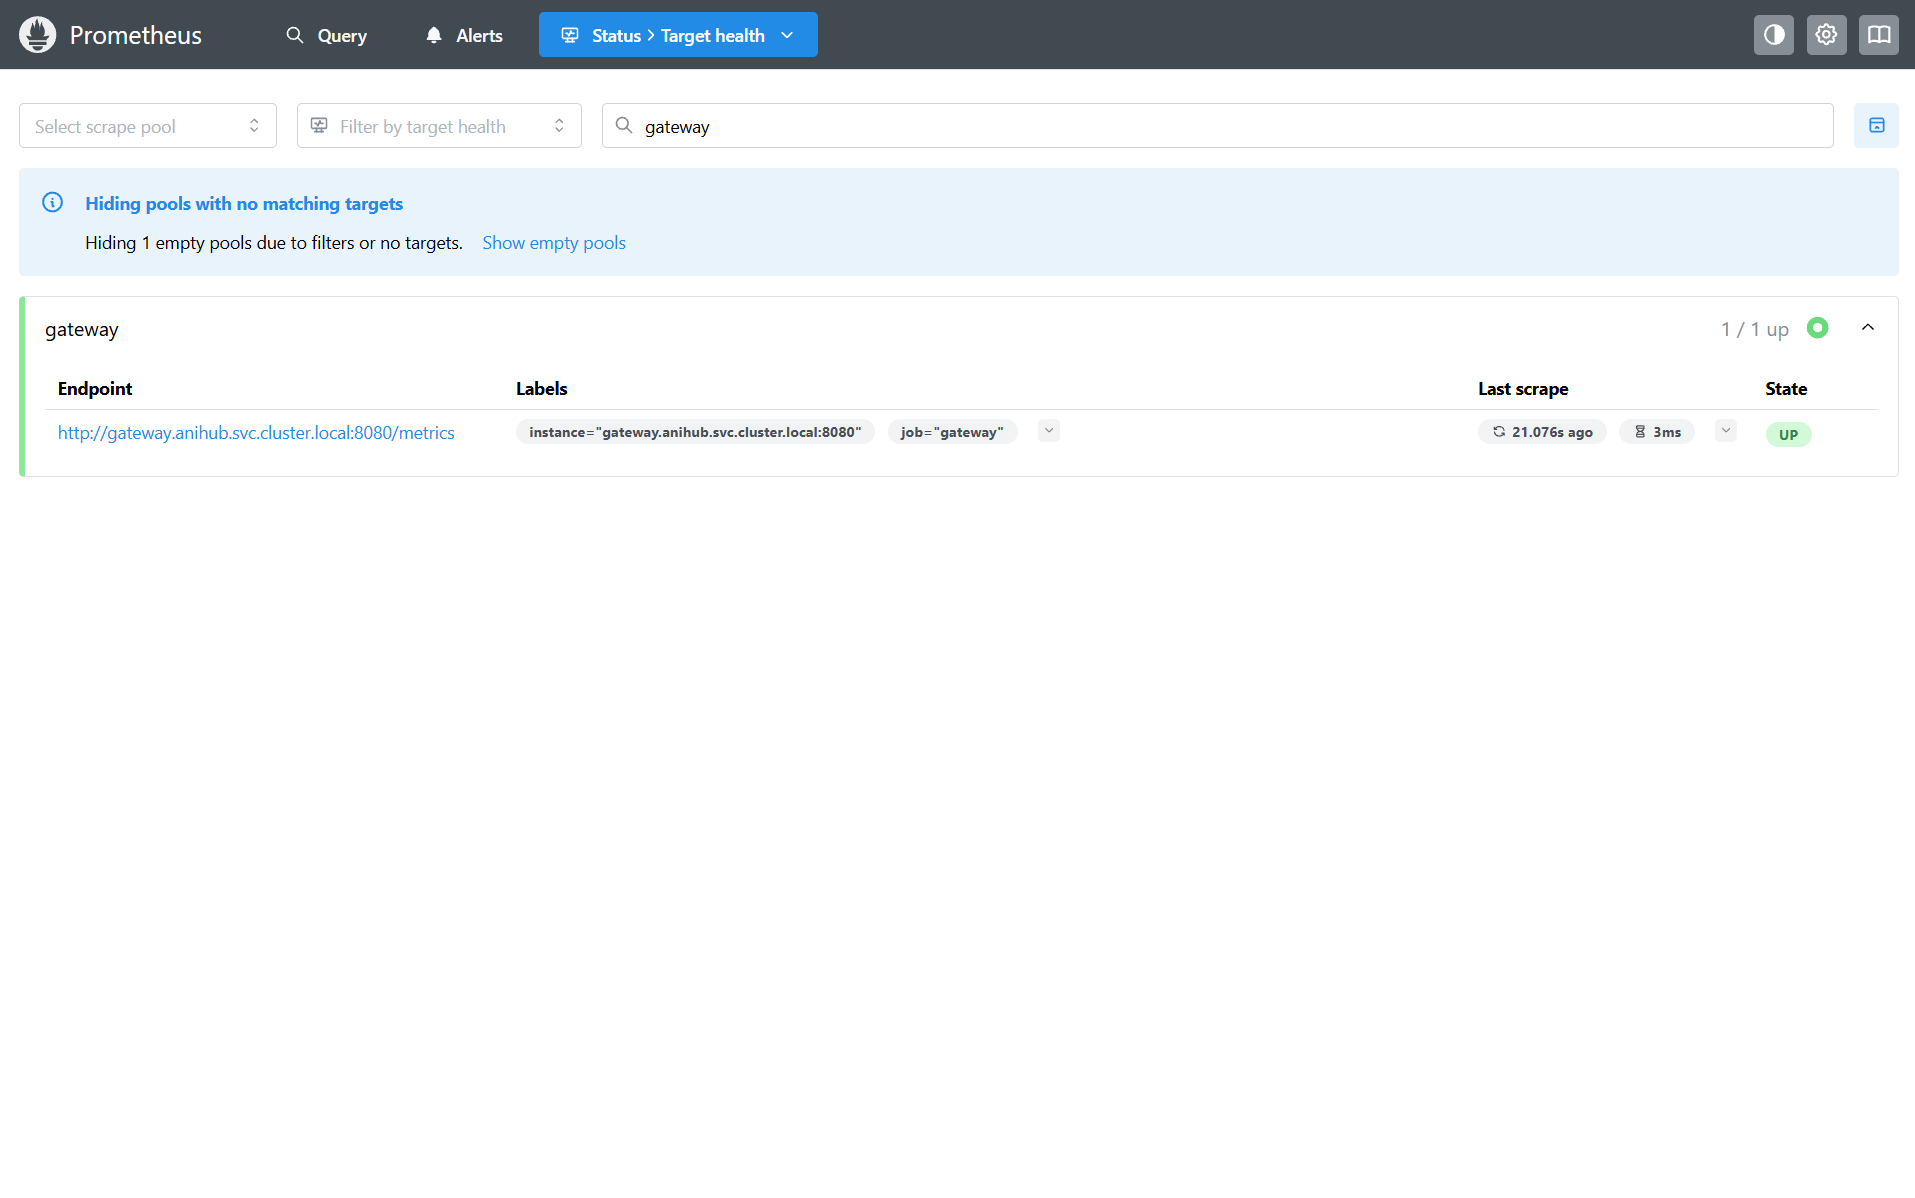
\includegraphics[width=0.5\linewidth]{images/prometheus target.png}
    \caption{Surveillance des microservices avec Prometheus}
    \label{fig:prometheus-monitoring}
\end{figure}
\newpage  
\subsubsection{Page de connexion de Grafana}

Cette figure illustre la page de connexion de Grafana permettant d’accéder à l’interface de monitoring des microservices et du cluster Kubernetes d’AniHub 
\begin{figure}[H]
    \centering
    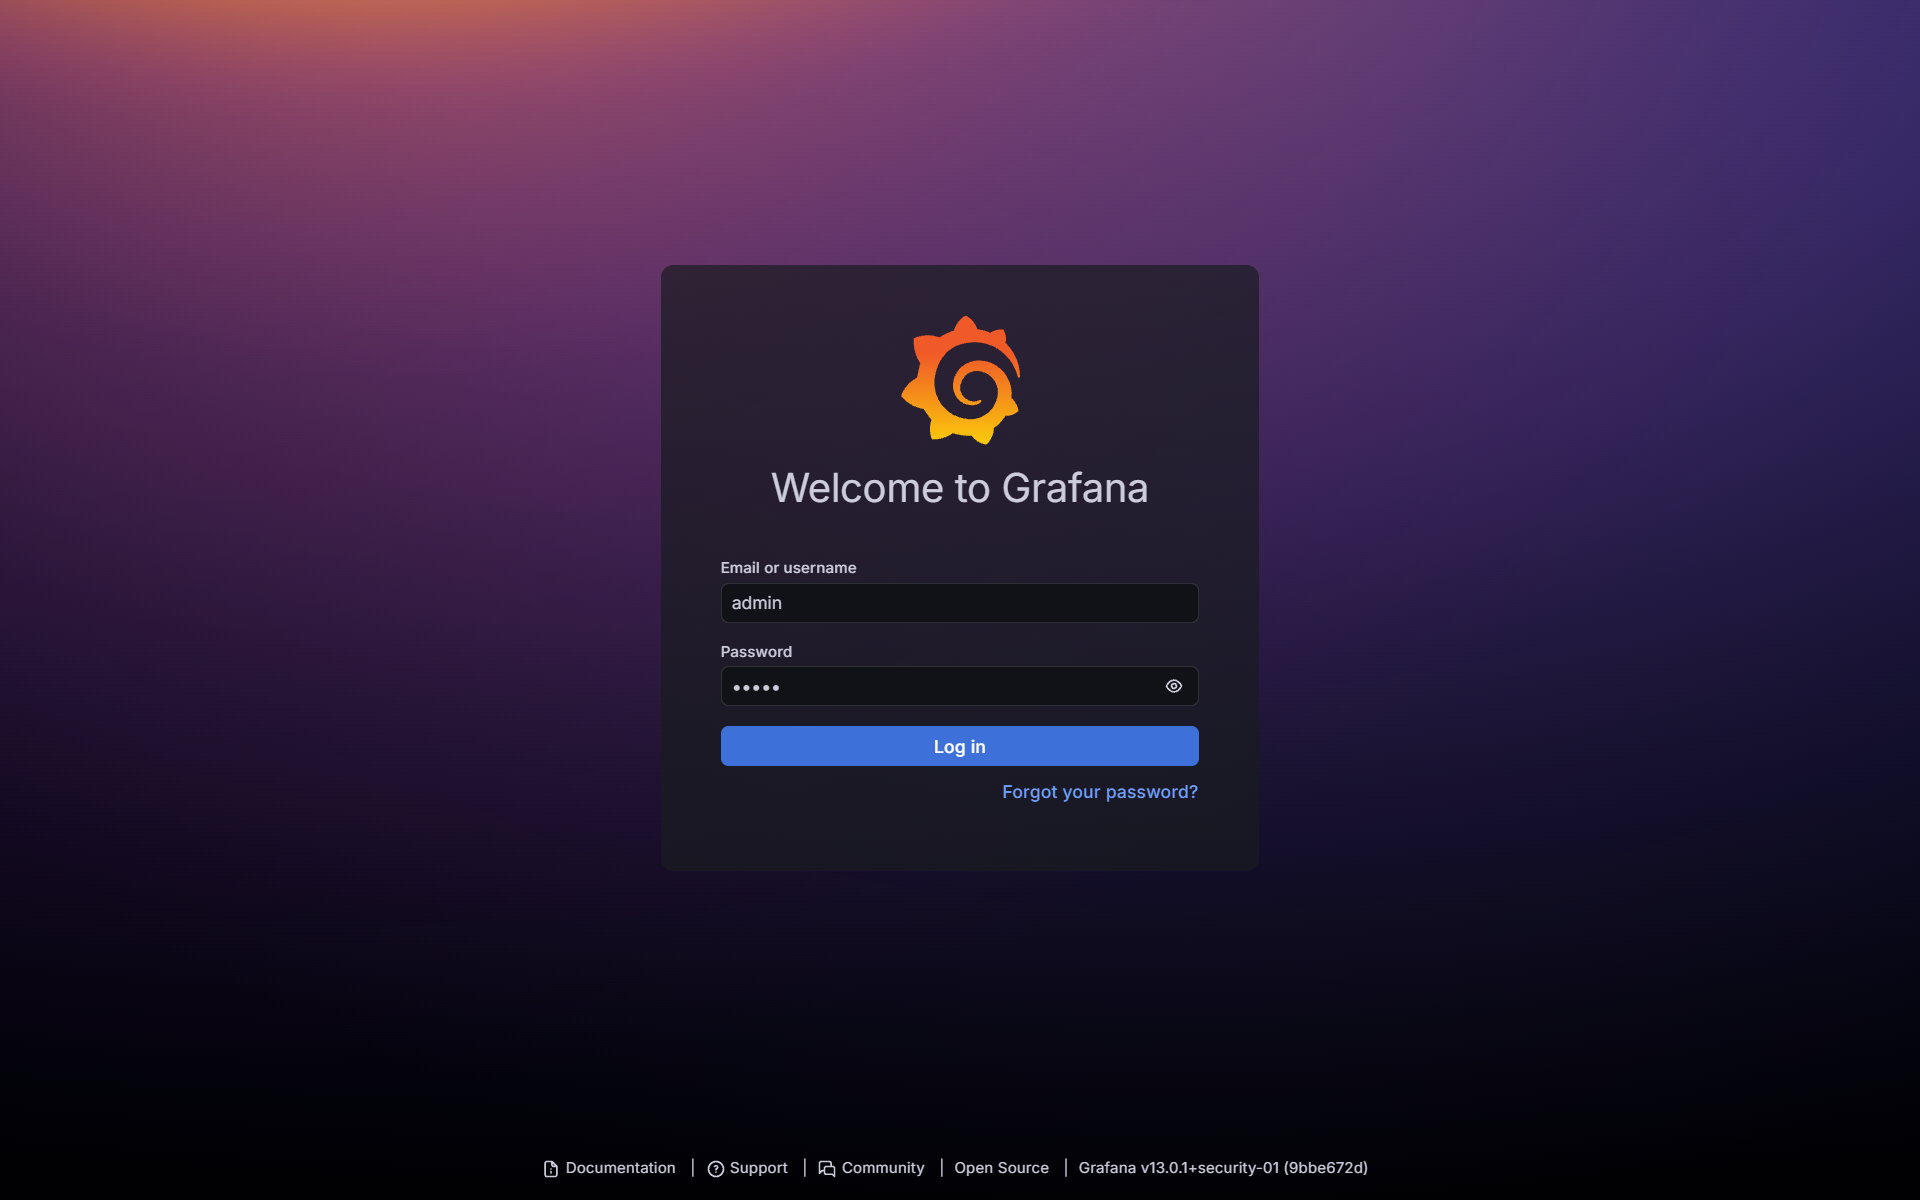
\includegraphics[width=0.6\linewidth]{images/grafana login.png}
    \caption{Page de connexion de Grafana}
    \label{fig:grafana-login}
\end{figure}  

\subsubsection{Tableau de bord Grafana : état de santé des microservices AniHub} 
Cette figure illustre un tableau de bord Grafana affichant l’état de santé des microservices d’AniHub : 
\begin{figure}[H]
    \centering
    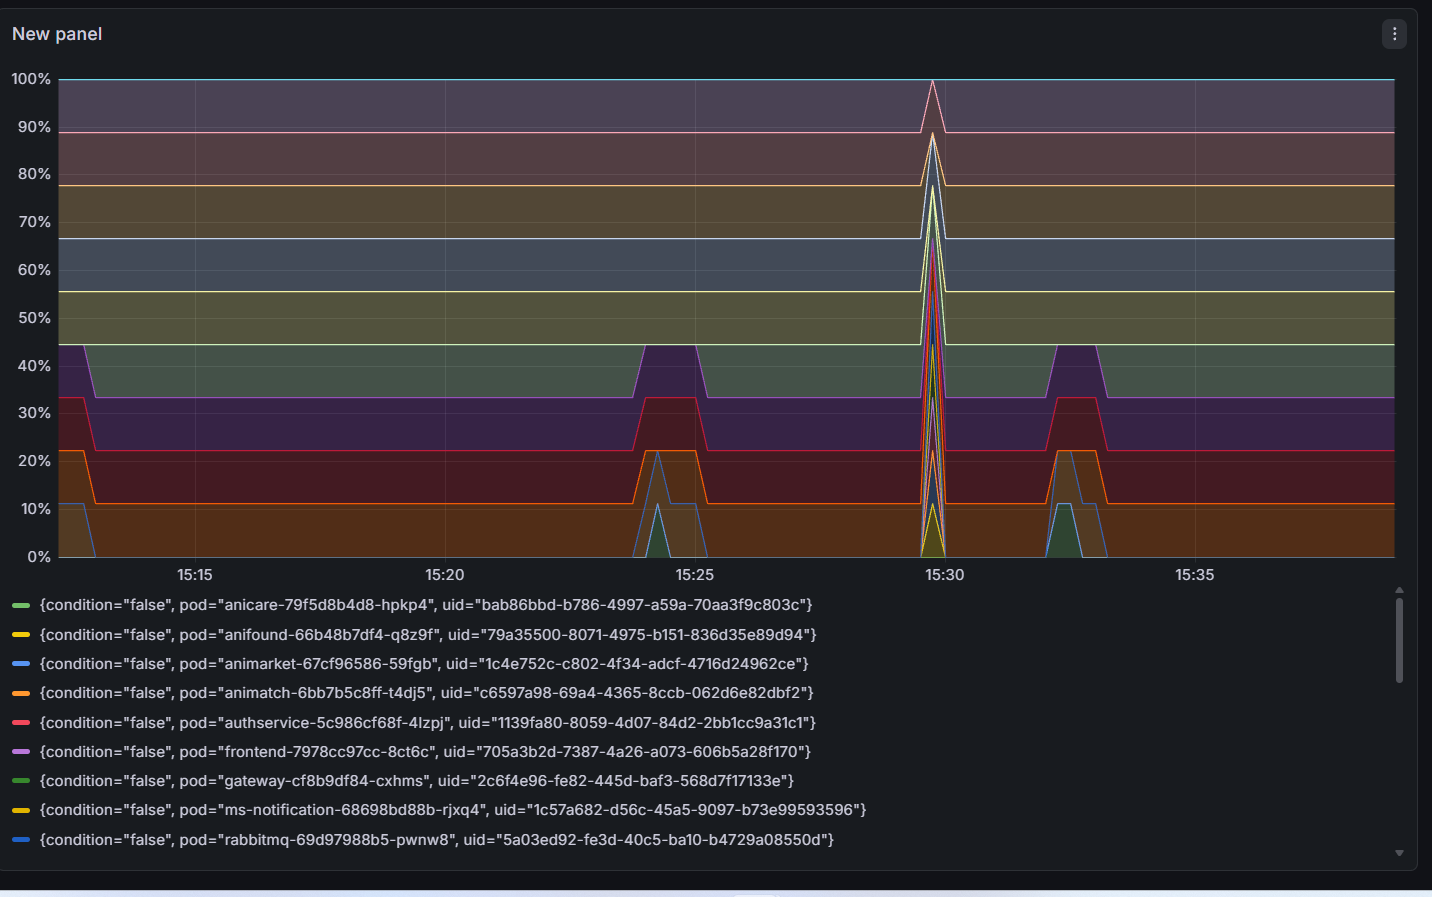
\includegraphics[width=0.9\linewidth]{images/etat de santé des microservices anihub grafana.png}
    \caption{Tableau de bord Grafana : état de santé des microservices AniHub}
    \label{fig:grafana-dashboard}
\end{figure} 
\newpage  


\subsubsection{Tableau de bord Grafana : Utilisation de la mémoire vive (RAM) par pod} 
Cette figure illustre la quantité de mémoire vive (RAM) actuellement consommée par chaque pod du namespace anihub, exprimée en octets : 
\begin{figure}[H]
    \centering
    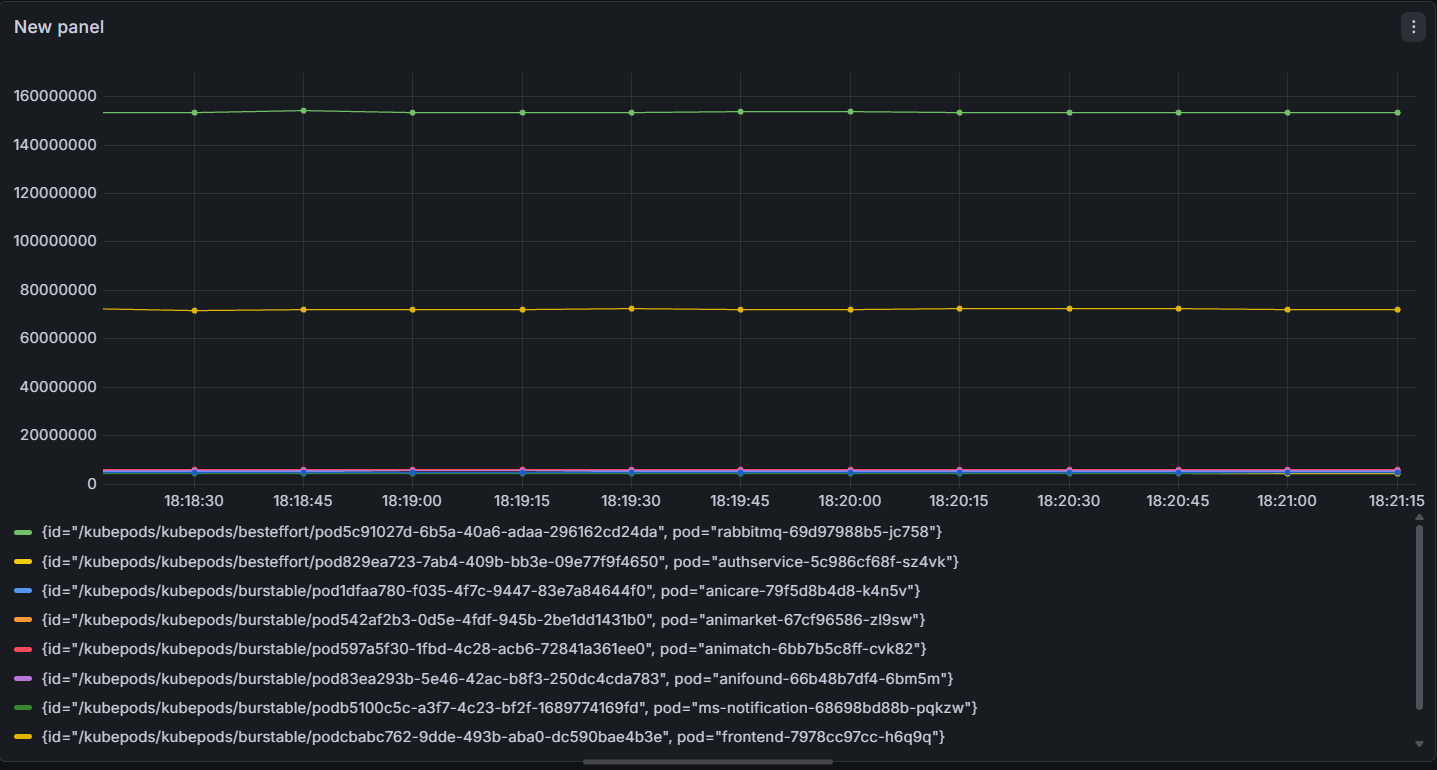
\includegraphics[width=0.8\linewidth]{images/consommation memoire ram.png}
    \caption{Tableau de bord Grafana : Utilisation de la mémoire vive (RAM) par pod}
    \label{fig:ram-usage}   
\end{figure}

\subsubsection{Tableau de bord Grafana : Consommation CPU des microservices AniHub} 
Cette figure illustre le taux d’utilisation du CPU par les microservices de la plateforme AniHub : 
\begin{figure}[H]
    \centering
    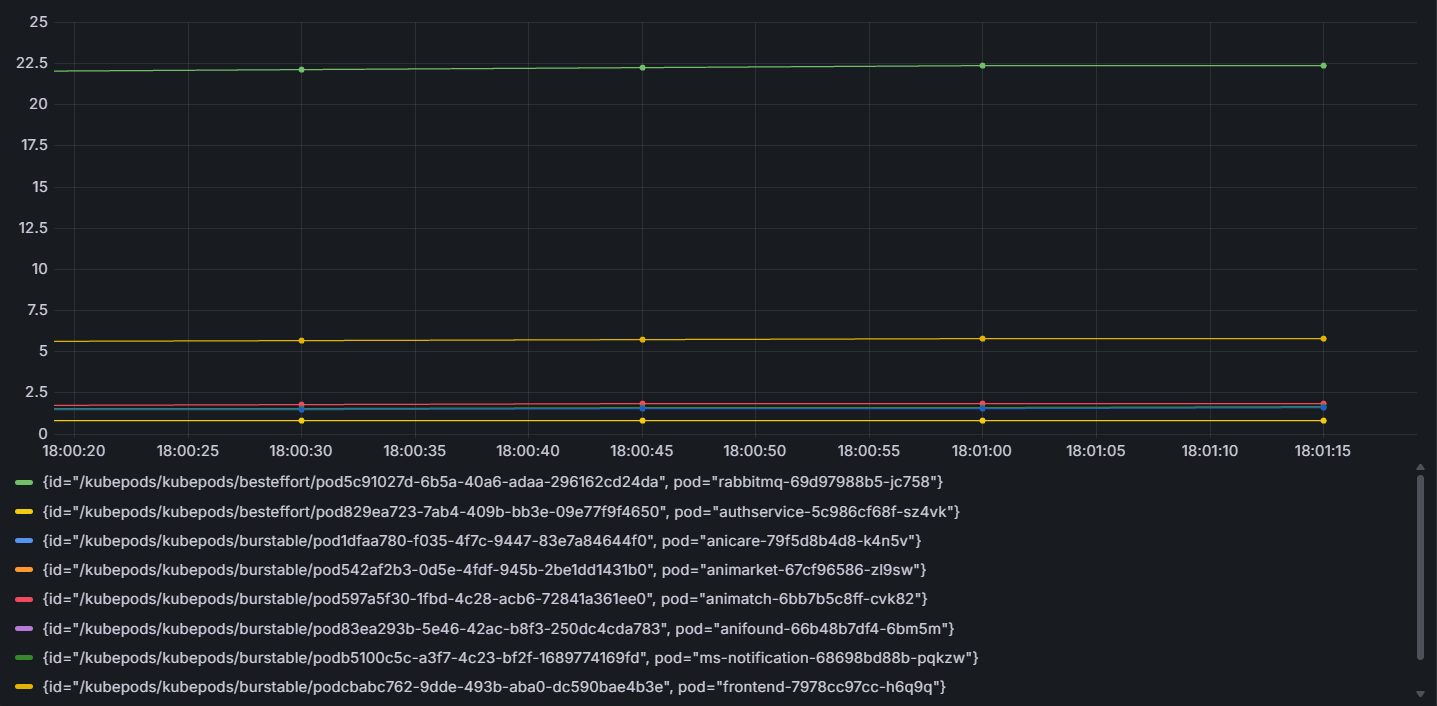
\includegraphics[width=0.8\linewidth]{images/consommation cpu.png}
    \caption{Tableau de bord Grafana : Consommation CPU des microservices AniHub}
    \label{fig:cpu-usage}   
\end{figure} 
\newpage

\subsubsection{Tableau de bord Grafana : Nombre de conteneurs actifs} 
Cette figure affiche le nombre total de conteneurs actuellement en cours d’exécution dans le namespace anihub. Au début, le nombre de conteneurs était de 9. Ensuite, afin de tester le mécanisme de scalabilité, le nombre de réplicas a été modifié à 2, ce qui a entraîné l’augmentation du nombre total de conteneurs à 18 : 
\begin{figure}[H]
    \centering
    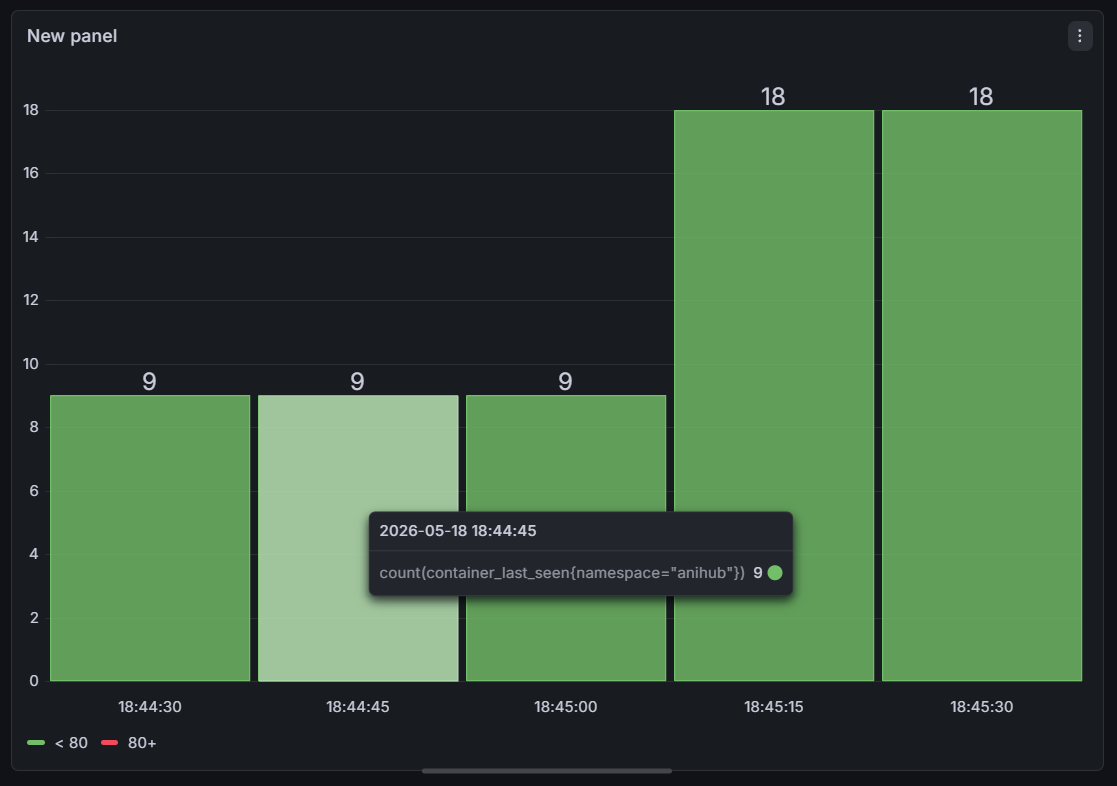
\includegraphics[width=0.7\linewidth]{images/Compteur de conteneurs actifs.png}
    \caption{Tableau de bord Grafana : Nombre de conteneurs actifs}
    \label{fig:containers-active}
\end{figure} 
\subsubsection{Tableau de bord grafana : État de santé de la Gateway} 
Cette figure illustre l’état de fonctionnement instantané de la Gateway, indiquant si elle est active ou indisponible à un instant donné : 
\begin{figure}[H]
    \centering
    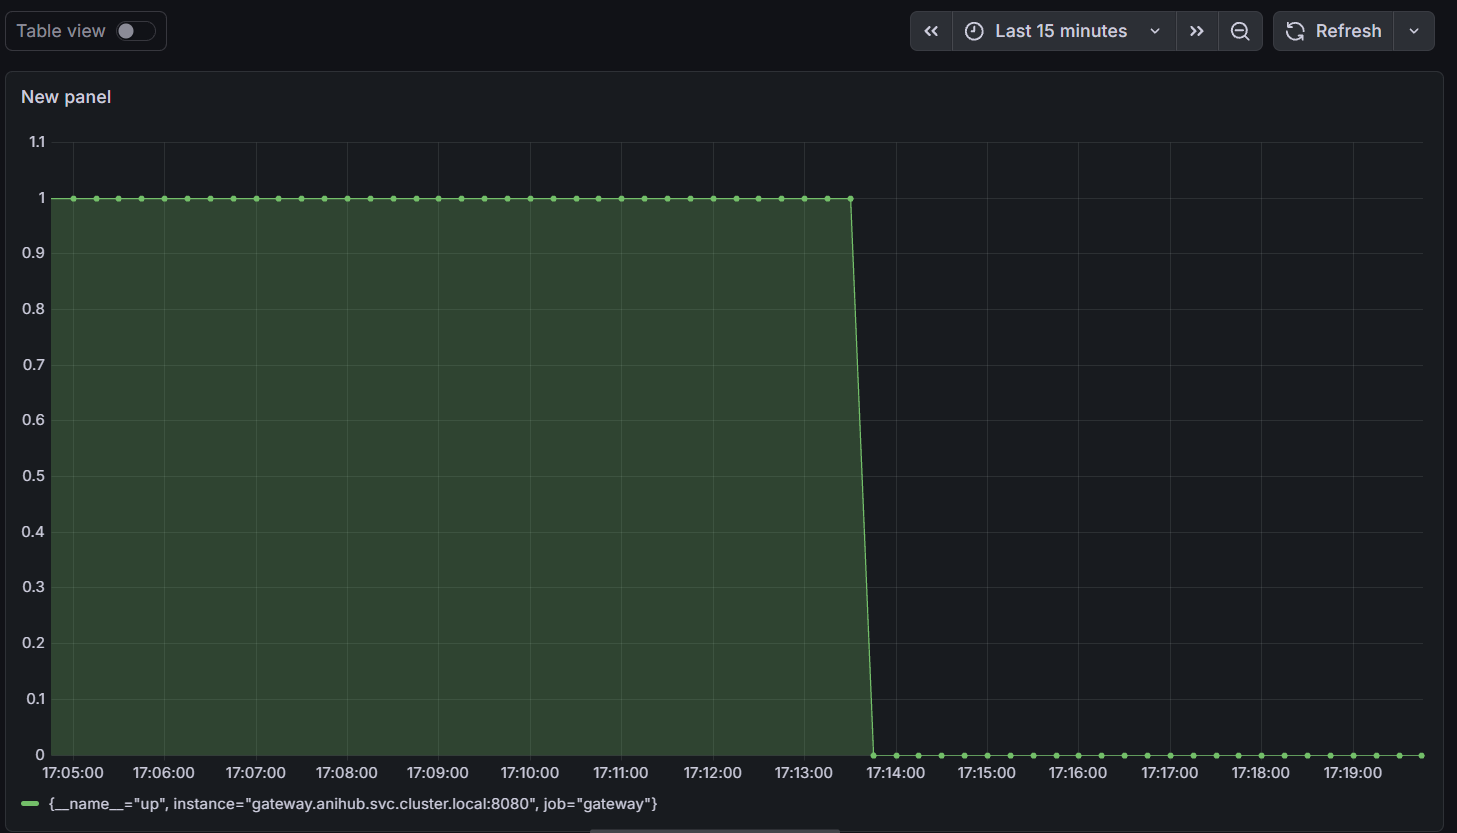
\includegraphics[width=0.7\linewidth]{images/etat de santé gateway.png}
    \caption{Tableau de bord Grafana : État de santé de la Gateway}
    \label{fig:gateway-health}
\end{figure}



\newpage
\subsubsection{Tableau de bord Grafana : Nombre de requêtes du microservice AniMatch} 
Cette figure illustre le nombre de requêtes HTTP du microservice AniMatch sur les deux dernières minutes, réparties selon les méthodes GET, POST, PUT et DELETE, afin d’analyser son activité et sa charge : 
\begin{figure}[H]
    \centering
    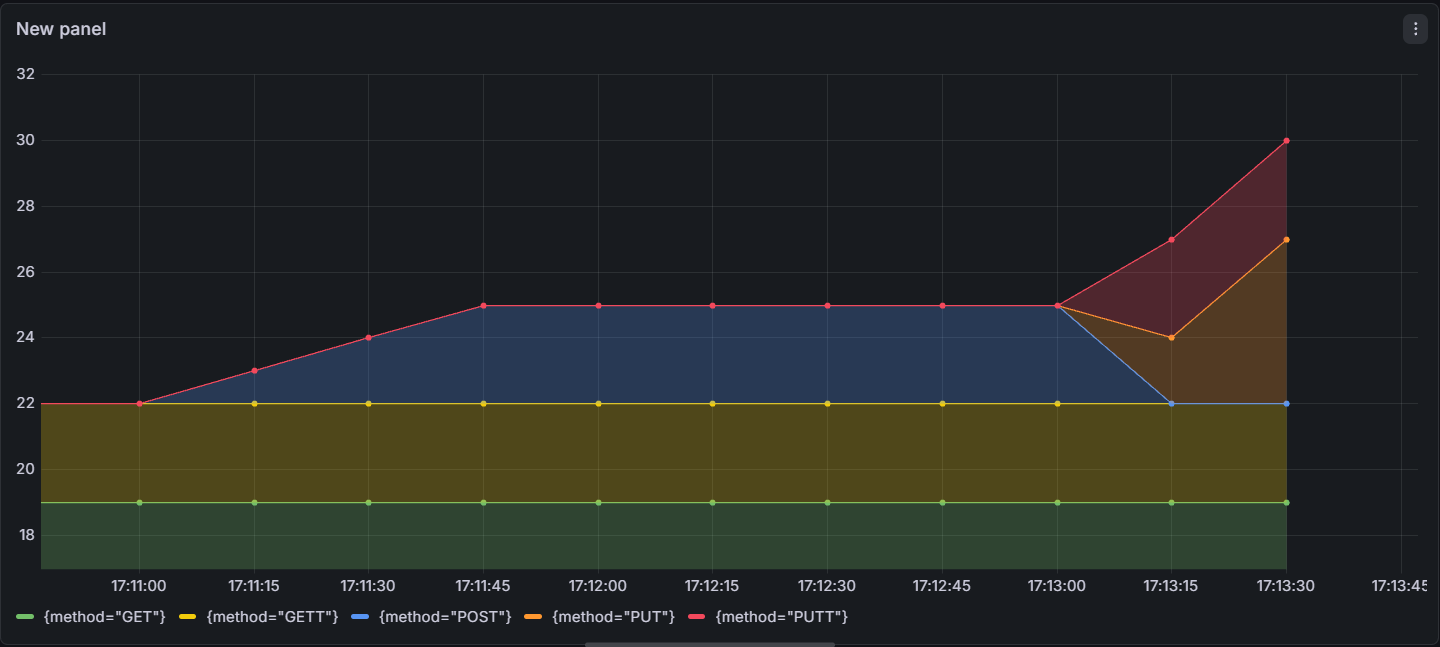
\includegraphics[width=0.9\linewidth]{images/nb requests vers animatch.png}
    \caption{Nombre de requêtes du microservice AniMatch(GET, POST, PUT, DELETE)}
    \label{fig:requests-animatch}
\end{figure}    
\subsubsection{Tableau de bord Grafana :Nombre de requêtes par microservices}
Cette figure illustre le nombre de requêtes traitées par chaque microservice de l’application AniHub, permettant d’analyser la charge et l’activité de chaque service : 

\begin{figure}[H]
    \centering
    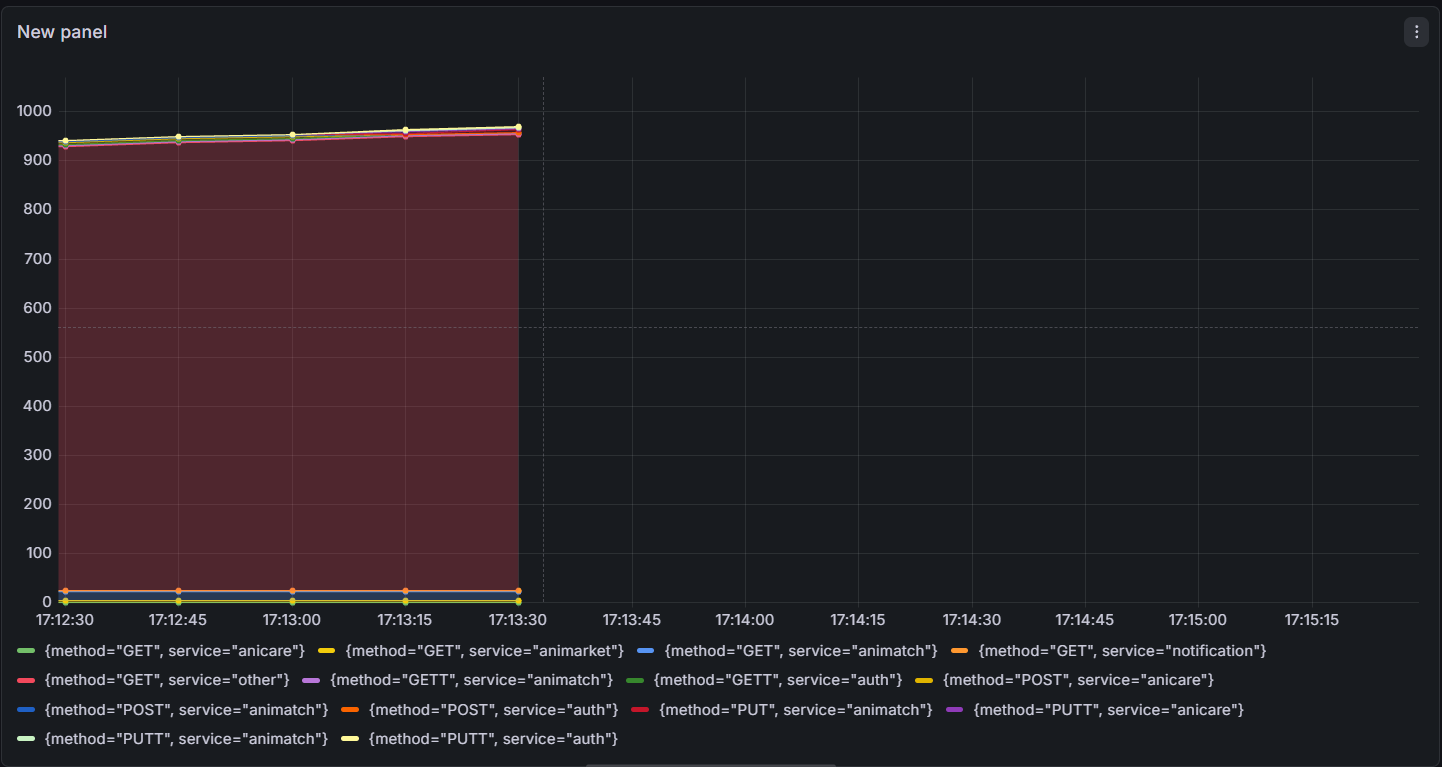
\includegraphics[width=0.9\linewidth]{images/nb requetes de services.png}
    \caption{Nombre de requêtes par microservices}
    \label{fig:requests-microservices}
\end{figure} 
\newpage






 

\chapter*{Conclusion et Perspectives}
\label{chap:conclusion}
\markboth{\MakeUppercase{Conclusion}}{}%
\addcontentsline{toc}{chapter}{Conclusion}
  And a very interesting conclusion here\@. ~\\
  Lorem ipsum dolor sit amet, consectetur adipisicing elit, sed do eiusmod
  tempor incididunt ut labore et dolore magna aliqua. Ut enim ad minim veniam,
  quis nostrud exercitation ullamco laboris nisi ut aliquip ex ea commodo
  consequat.

\newpage
\appendix
\addcontentsline{toc}{chapter}{Annexes}
%\markboth{\MakeUppercase{Annexe}}{}

\chapter{Code R pour résoudre la problématique}
\label{chap:appendix}


\section{Pré-traitement des données}
\section{Code R pour les modèles}

 An appedix if you need it.
 
 \begin{verbatim}
 Insérer ici le code !
 \end{verbatim}

\section{Librairies utilisées}
 
  Lorem ipsum dolor sit amet, consectetur adipisicing elit, sed do eiusmod
  tempor incididunt ut labore et dolore magna aliqua. Ut enim ad minim veniam,
  quis nostrud exercitation ullamco laboris nisi ut aliquip ex ea commodo.


%%%%%%%%%%%%%%%%%%%%%%%%%%%%%%%%%%%%%%%%%%%%%%%%%%%%
% Don't touch this, it is auto generated
%%%%%%%%%%%%%%%%%%%%%%%%%%%%%%%%%%%%%%%%%%%%%%%%%%%%
\nocite{*}

%\phantomsection{}
%\addcontentsline{toc}{chapter}{Webography}
%\printbibliography[title={Webography},type=online]

%\phantomsection{}
%\addcontentsline{toc}{chapter}{Bibliography}
%\printbibliography[title={Bibliography},nottype=online]

%\printbibheading %exemple de bibliographie divisée en sections. Pour ajouter des oeuvres non citées,utiliser \nocite

%\printbibliography[keyword=pratique,heading=subbibliography,title={Théories littéraires dans les jeux vidéo}]
%\printbibliography[keyword=litteraire,heading=subbibliography,title={Narratologie et structuralisme}]

%\printbibliography[keyword=jeu,heading=subbibliography,title={\emph{Games studies}}]



\cleardoublepage%

\addtocontents{toc}{\protect\setcounter{tocdepth}{3}}

\printglossaries
\printindex



\begin{abstract}

aThe present work is part of a graduation project carried out within the company \studyDepartment in order to obtain the national diploma of engineer at the \ITBS. This project's objective is to design and implement a ... \\
% les tests de performance 
%\keywords{}
\keywordss{} \\

\vspace{3cm}
\centerline{\bf Résumé}
\vspace{0.6cm}

aCe travail s’inscrit dans le cadre du projet de fin d’études réalisé au sein de \studyDepartment en vue de l’obtention du diplôme national d’ingénieur à l’\ITBS. L’objectif de ce projet consiste à ... \\


\keywords{}
%\keywordss{}
\end{abstract}


\chapter*{Références Netographiques}
\addcontentsline{toc}{chapter}{Références Netographiques}

\bibliographystyle{unsrt}
\bibliography{references}
\end{document}
